\documentclass[11pt]{article}
% Freeze reproducibility: suppress pdfTeX's build-directory-dependent trailer ID.
\ifdefined\pdftrailerid\pdftrailerid{}\fi
\usepackage[a4paper,margin=1in]{geometry}
\usepackage[utf8]{inputenc}
\usepackage[T1]{fontenc}
\usepackage{lmodern}
\usepackage{amsmath,amssymb,mathtools}
\usepackage{microtype}
\usepackage{graphicx}
\usepackage{tikz}
\usepackage{enumitem}
\usepackage{longtable,booktabs,array}
\usepackage{fancyhdr}
\setlength{\parindent}{1.5em}
\setlength{\parskip}{0.25em}
\setlength{\headheight}{14pt}
\sloppy
\hbadness=10000
\hfuzz=100pt
\vfuzz=100pt
\newcommand{\oldquote}{\par\begingroup\leftskip=1.6em\rightskip=0.8em\noindent}
\newcommand{\closeoldquote}{\par\endgroup}
\newcommand{\diff}{\mathrm{d}}
\newcommand{\detmat}[1]{\left|\begin{matrix}#1\end{matrix}\right|}
% Added in p0505-p0543 final tranche for source-style two-row Christoffel symbols.
\providecommand{\Ctwo}[2]{\left\{\begin{matrix}#1\\#2\end{matrix}\right\}}
\providecommand{\cotg}{\operatorname{cotg}}

\pagestyle{plain}
\allowdisplaybreaks

% Source-style footnote marks: preserve scan-visible parenthesized markers.
\makeatletter
\newcommand{\srcfnmark}[1]{\textsuperscript{(#1)}}
\newcommand{\srcfntext}[2]{%
  \begingroup
  \def\@thefnmark{(#1)}%
  \@footnotetext{#2}%
  \endgroup
}
\newcommand{\srcfn}[2]{%
  \begingroup
  \def\@thefnmark{(#1)}%
  \@footnotemark
  \@footnotetext{#2}%
  \endgroup
}
\makeatother


\DeclareMathOperator{\sen}{sen}
\DeclareMathOperator{\tg}{tg}

\DeclareMathOperator{\senh}{senh}
\DeclareMathOperator{\cn}{cn}
\DeclareMathOperator{\sn}{sn}
\DeclareMathOperator{\dn}{dn}
\DeclareMathOperator{\arc}{arc}
\DeclareMathOperator{\sett}{sett}
\DeclareMathOperator{\tgh}{tgh}



\newcommand{\chr}[3]{\left\{\begin{matrix}#1#2\\#3\end{matrix}\right\}}
\newcommand{\chrsq}[3]{\left[\begin{matrix}#1#2\\#3\end{matrix}\right]}

% Current-slice two-row Christoffel symbol macros, kept distinct from the older three-argument macros.
\providecommand{\chrB}[2]{\left\{\begin{matrix}#1\\#2\end{matrix}\right\}}
\providecommand{\chrsqB}[2]{\left[\begin{matrix}#1\\#2\end{matrix}\right]}

\newcommand{\chrfour}[2]{\left\{#1,#2\right\}}
\newcommand{\bigdet}[1]{\left|\begin{matrix}#1\end{matrix}\right|}
\newcommand{\dd}{\,d}

\renewcommand{\srcfnmark}[1]{\ifmmode{}^{(#1)}\else\textsuperscript{(#1)}\fi}

% Additional operators encountered in source pdfpages 0281-0312.
\providecommand{\tgh}{\operatorname{tgh}}
\providecommand{\tang}{\operatorname{tang}}
\providecommand{\tangh}{\operatorname{tangh}}
\providecommand{\coth}{\operatorname{coth}}

\newcommand{\figseven}{%
\begin{center}\begin{minipage}{.95\linewidth}\centering
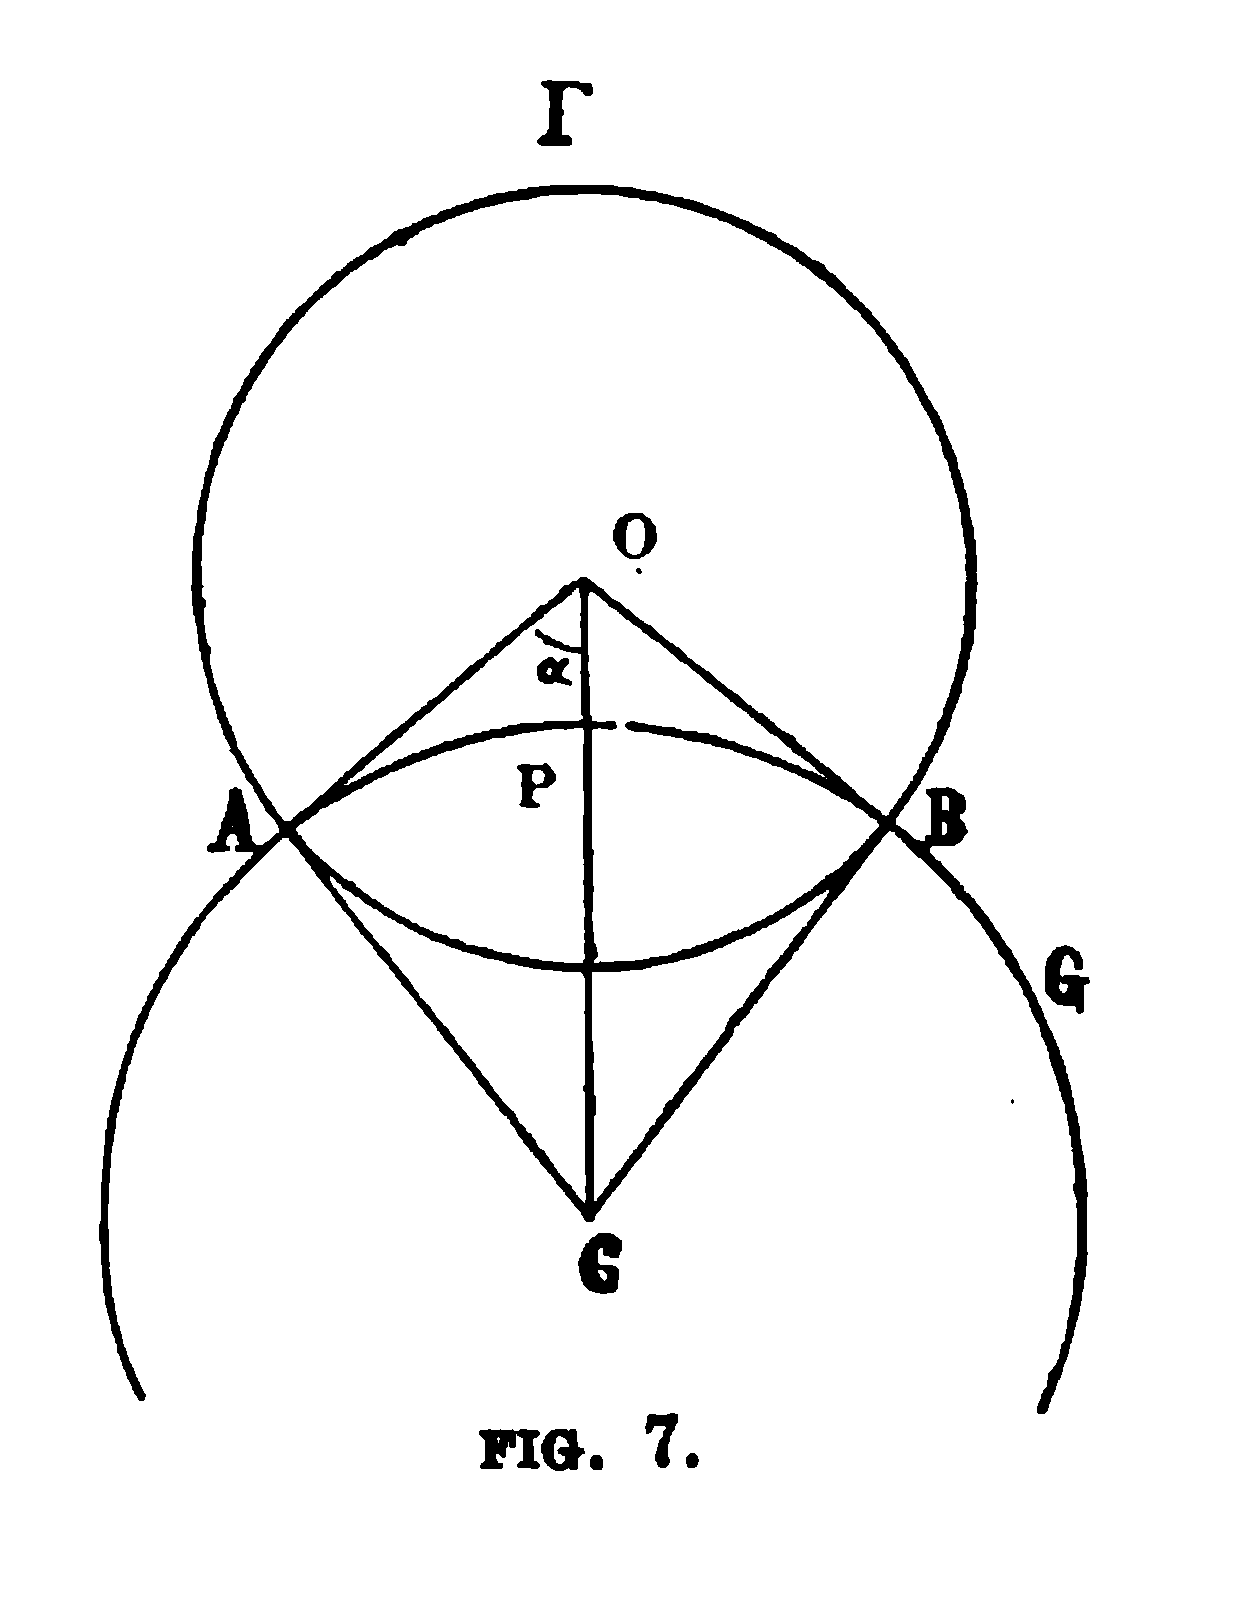
\includegraphics[width=.38\linewidth]{assets/ch12_facsimiles/embedded/Luigi_Bianchi_Geometria_differenziale_Figura_7_facsimile.png}
\end{minipage}\end{center}}
\newcommand{\figsevena}{%
\begin{center}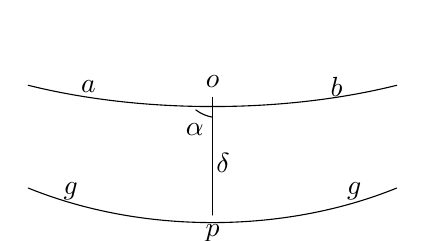
\begin{tikzpicture}[scale=0.9,line cap=round,line join=round]
\draw (-2.6,.65) .. controls (-1,.25) and (1,.25) .. (2.6,.65);
\draw (-2.6,-.8) .. controls (-1,-1.45) and (1,-1.45) .. (2.6,-.8);
\draw (0,.48)--(0,-1.18); \node[above] at (0,.48) {$o$}; \node[below] at (0,-1.18) {$p$};
\node at (-1.75,.63) {$a$}; \node at (1.75,.63) {$b$}; \node at (-2.0,-.85) {$g$}; \node at (2.0,-.85) {$g$};
\draw (0,.2) arc (260:233:.55); \node at (-.25,.03) {$\alpha$}; \node at (.15,-.45) {$\delta$};
\end{tikzpicture}\\[-.2em]{\small Fig. 7a.}\end{center}}
\newcommand{\figeight}{%
\begin{center}\begin{minipage}{.95\linewidth}\centering
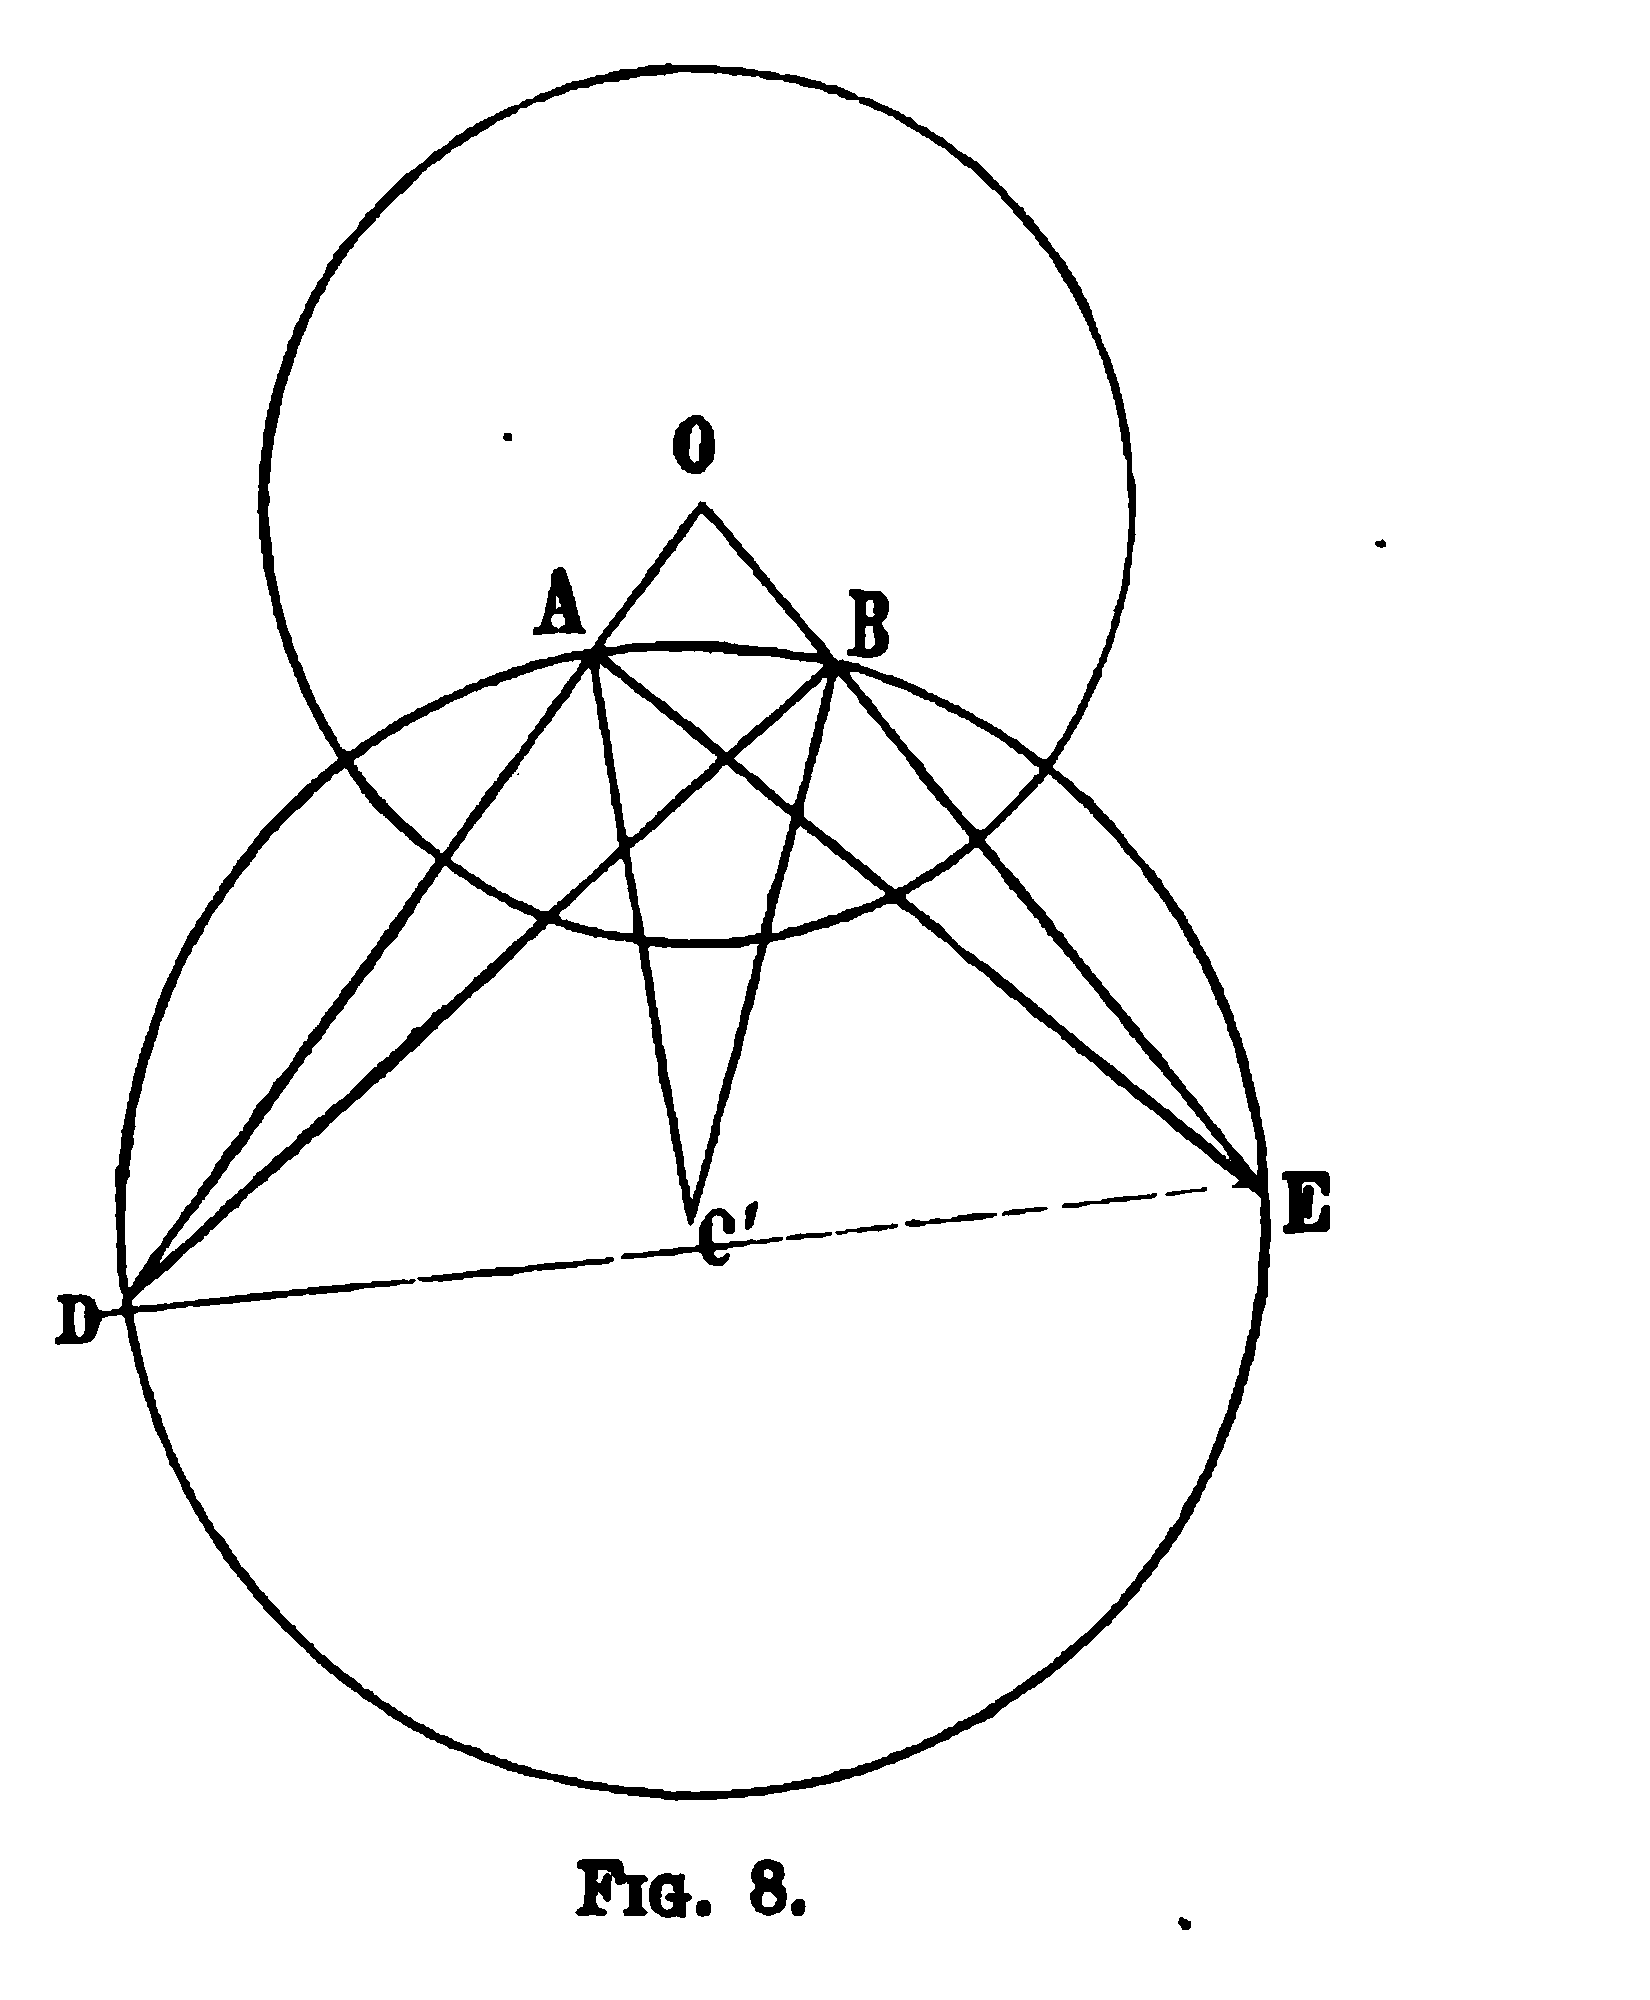
\includegraphics[width=.42\linewidth]{assets/ch12_facsimiles/embedded/Luigi_Bianchi_Geometria_differenziale_Figura_8_facsimile.png}
\end{minipage}\end{center}}
\newcommand{\fignine}{%
\begin{center}\begin{minipage}{.95\linewidth}\centering
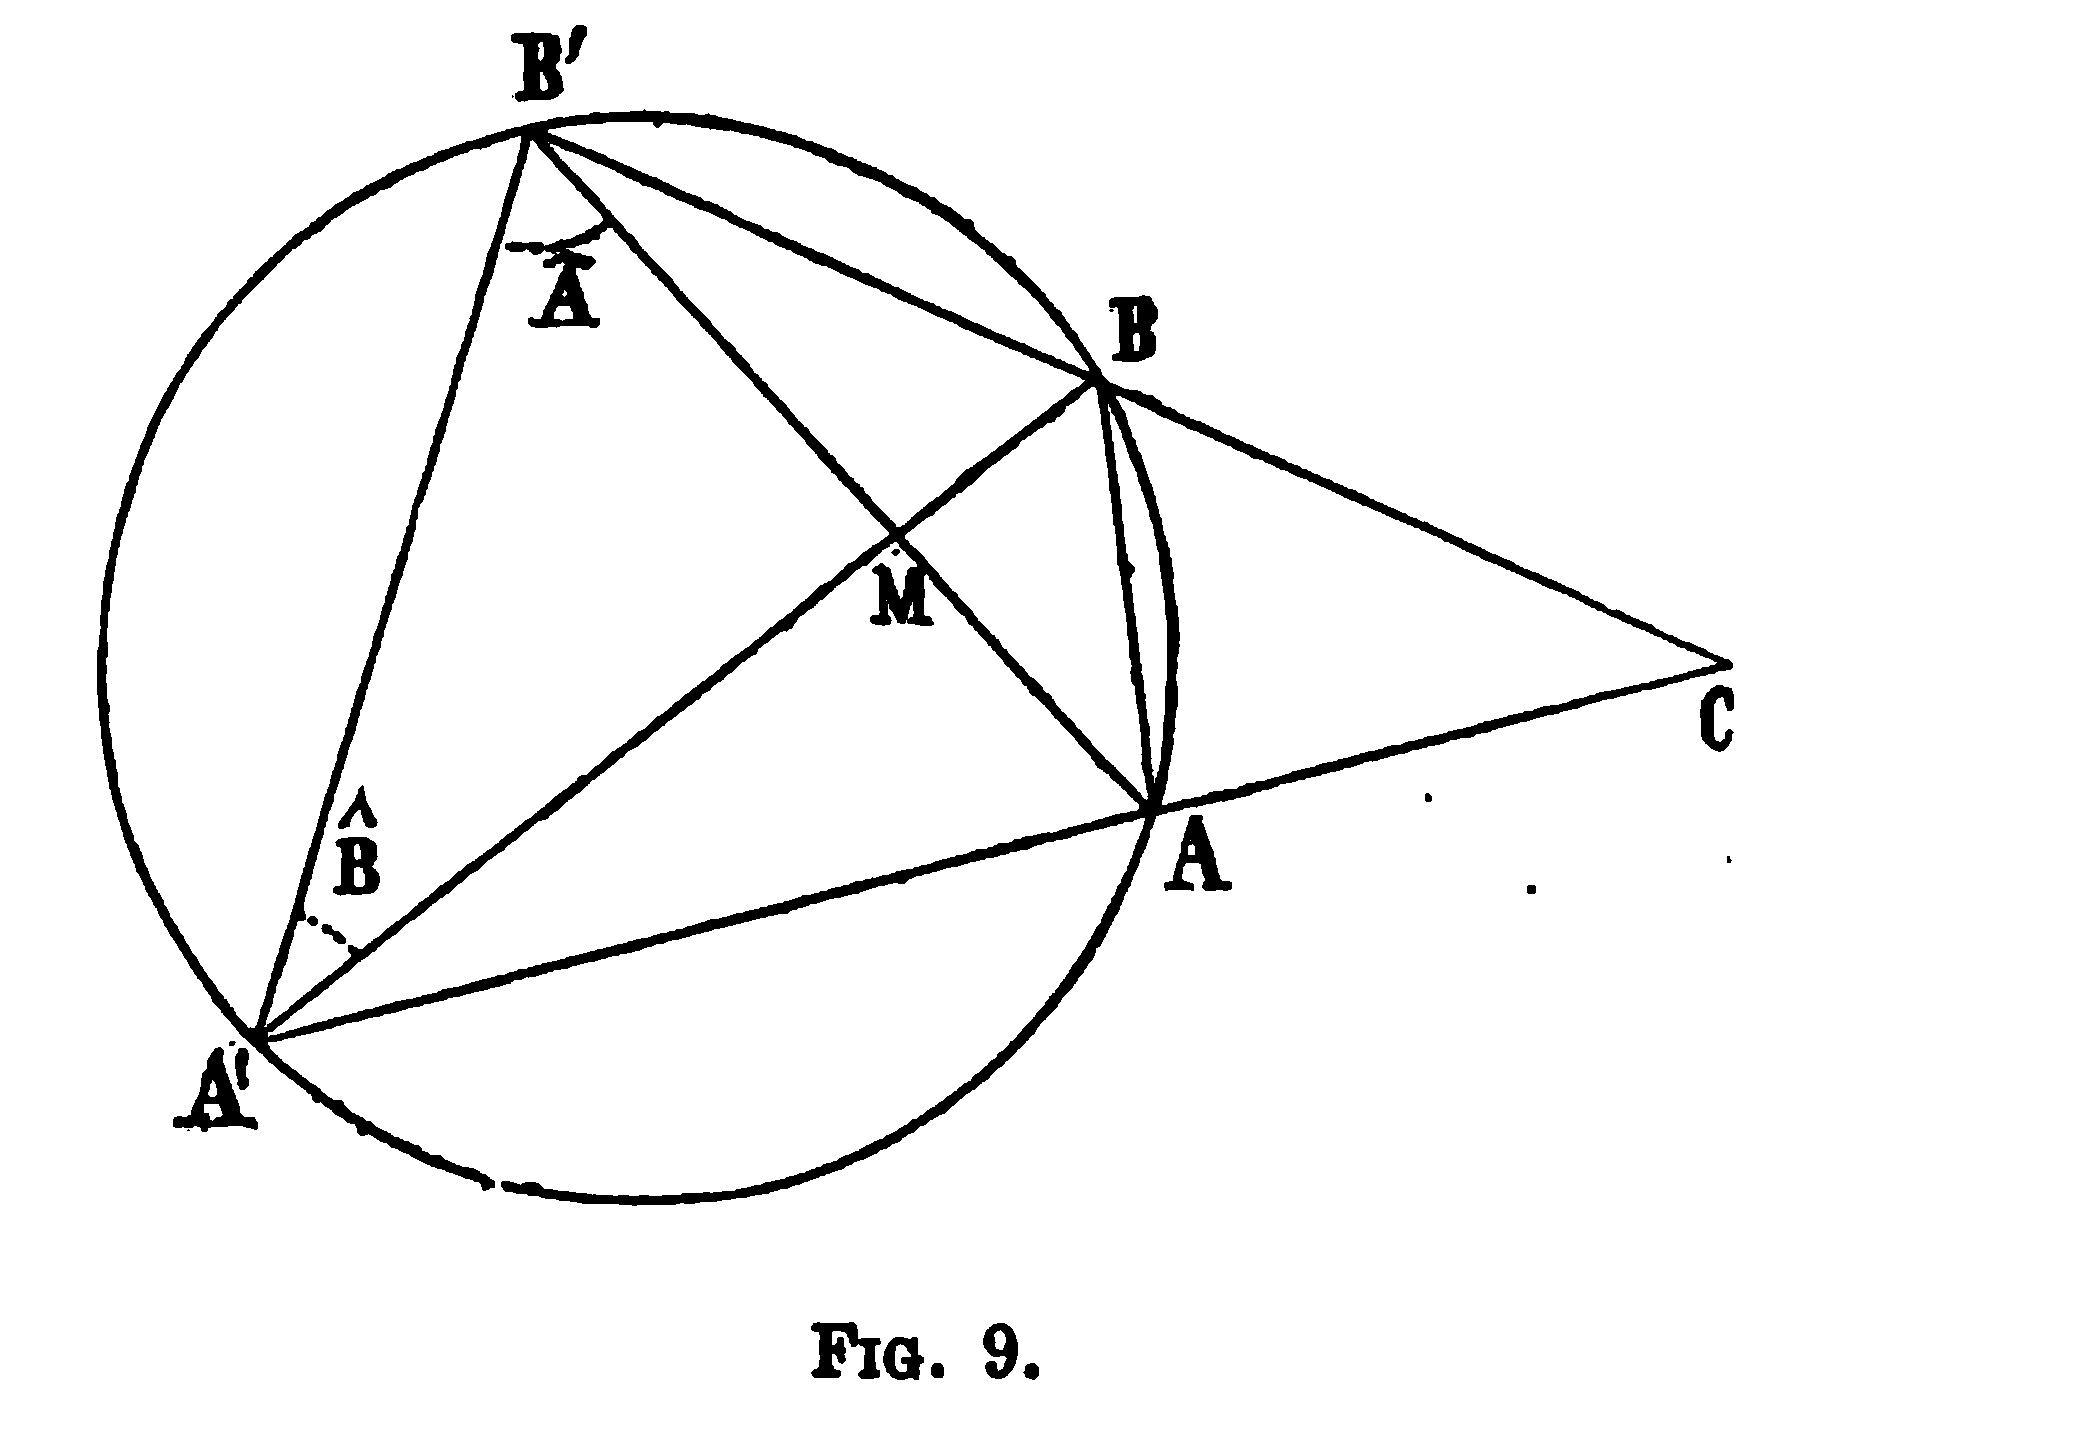
\includegraphics[width=.54\linewidth]{assets/ch12_facsimiles/embedded/Luigi_Bianchi_Geometria_differenziale_Figura_9_facsimile.png}
\end{minipage}\end{center}}


% compatibility shims for p0409--0440 continuation
\providecommand{\sen}{\operatorname{sen}}
\providecommand{\tg}{\operatorname{tg}}
\providecommand{\senh}{\operatorname{senh}}
\providecommand{\tgh}{\operatorname{tgh}}
\providecommand{\cotgh}{\operatorname{cotgh}}
\providecommand{\ang}{\operatorname{ang}}
\providecommand{\grad}{\operatorname{grad}}
\providecommand{\chrB}[2]{\left\{\begin{matrix}#1\\#2\end{matrix}\right\}}
\providecommand{\chrsqB}[2]{\left[\begin{matrix}#1\\#2\end{matrix}\right]}

\begin{document}


\begin{center}
{\bfseries LUIGI BIANCHI}\par
{\small PROFESSORE DELLA REGIA UNIVERSITÀ DI PISA}\par
\vspace{1.5em}
{\Huge\bfseries LEZIONI}\par
\vspace{1em}
DI\par
\vspace{1em}
{\LARGE\bfseries GEOMETRIA DIFFERENZIALE}\par
\vspace{1em}
Seconda edizione riveduta e considerevolmente aumentata\par
{\bfseries IN DUE VOLUMI}\par
\vspace{1.25em}
{\large\bfseries VOLUME I.}\par
\vspace{4em}
{\large PISA}\par
{\bfseries ENRICO SPOERRI}\par
{\scriptsize LIBRAIO-EDITORE}\par
1902
\end{center}

\begin{center}
{\small Pisa, Tipografia Successori Fratelli Nistri, 1902}
\end{center}

\section*{PREFAZIONE}
Dimostratasi l'opportunità di una seconda edizione del presente trattato, ho stimato utile, pur conservando nelle sue linee fondamentali il disegno generale dell'opera, di accrescerne notevolmente le proporzioni, per modo che non poche parti della teoria, costrette prima in troppo angusto spazio, venissero a trovare nella nuova trattazione un più adeguato sviluppo. E diversi nuovi capitoli ho aggiunto sia per trattare teorie relativamente già antiche, ma che non poterono venire accolte nella prima edizione, sia per far conoscere quelle ricerche di data affatto recente che segnano, come sembra, i più notevoli progressi fatti dalla geometria infinitesimale negli ultimi tempi.

La mole dell'opera per tal modo raddoppiata ha reso necessaria la divisione in due volumi, ed ho cercato che ciò corrisponda all'incirca alla divisione delle teorie in generali e speciali.

Il presente primo volume consta di quattordici capitoli, dei quali i primi dieci riproducono, con molte variazioni ed aggiunte, i capitoli corrispondenti della prima edizione, dalla quale tolgo ancora le seguenti avvertenze.

\oldquote
« Il metodo a cui il presente corso è totalmente informato ripete le sue origini dalle celebri \emph{Disquisitiones generales circa superficies curvas} di Gauss, e consiste nel riguardare la geometria infinitesimale come lo studio di una forma differenziale quadratica, o di due tali forme simultanee. Per ciò, dopo un primo capitolo che tratta delle curve a doppia curvatura, si troverà un secondo capitolo ove sono esposti, in tutta brevità, i fondamenti della teoria delle forme differenziali quadratiche.
\closeoldquote

\oldquote
Gli algoritmi che da questa teoria derivano hanno il grande vantaggio di dare alle formole un aspetto semplice ed elegante, che facilmente si imprime nella memoria, pur conservando alle linee coordinate tutta la loro generalità; essi vengono usati costantemente nel seguito del libro a cui questo capitolo serve di preliminare.

Lo studio generale delle superficie, e cioè tanto delle proprietà inerenti alla loro forma effettiva nello spazio quanto di quelle invariabili per flessione delle superficie (teoria dell'applicabilità) si trova esposto nei seguenti sette capitoli (III--IX). Il capitolo X tratta la teoria generale dei sistemi doppiamente infiniti di raggi (congruenze), teoria tanto importante per lo studio generale delle superficie e alla quale la geometria infinitesimale deve molti dei suoi risultati più notevoli. »
\closeoldquote

I quattro capitoli seguenti riproducono, con maggiori sviluppi e numerose aggiunte, l'esposizione dei principî fondamentali della geometria infinitesimale a \(n\) dimensioni che ho già dato nell'edizione tedesca del libro\footnote{\emph{Vorlesungen über Differentialgeometrie} deutsch von M. Lukat (Teubner, Leipzig 1899).}. Il capitolo XI, poste le convenzioni fondamentali per la metrica lineare ed angolare di uno spazio qualunque a \(n\) dimensioni, introduce la nozione di curvatura Riemanniana e generalizza alle curve ed alle ipersuperficie le formole della ordinaria teoria, con particolare riguardo alle proprietà delle linee di curvatura.

Passo poi a trattare più particolarmente degli spazî a curvatura Riemanniana costante; e mi occupo dapprima nel Cap. XII (che corrisponde al Capitolo XVI della prima edizione) della geometria pseudosferica a due dimensioni, con un breve cenno sulla geometria non-euclidea.

Nel seguente Cap. XIII studio in generale la geometria degli spazî a \(n\) dimensioni di curvatura costante, introduco la metrica del Cayley ed il sistema di coordinate del Weierstrass e mi occupo particolarmente della rappresentazione analitica e delle proprietà dei movimenti negli spazî a tre dimensioni, per terminare coll'importante nozione del paral-

\noindent lelismo di Clifford nello spazio ellittico e coll'estensione delle formole di Frenet per le curve alla geometria ellittica ed iperbolica.

In fine nel Cap. XIV vengono applicate le teorie generali allo studio delle ipersuperficie negli spazî a \(n\) dimensioni di curvatura costante, con particolare riguardo al caso delle tre dimensioni, ove vengono estesi tutti i principali risultati già noti per lo spazio euclideo.

Al collega prof. O. Niccoletti, che gentilmente mi coadiuvò nell'ultima revisione delle prove di stampa, rendo qui le più sincere grazie.

\begin{flushleft}
\emph{Pisa, Aprile 1902.}
\end{flushleft}

\section*{CAPITOLO I.}
\begin{center}
{\Large\bfseries Curve a doppia curvatura}
\end{center}

\begin{center}\footnotesize
Tangente e piano normale. -- Prima curvatura o flessione. -- Piano osculatore. -- Triedro principale. -- Seconda curvatura o torsione. -- Formole di Frenet. -- Equazioni intrinseche. -- Eliche cilindriche. -- Superficie inviluppi. -- Superficie canali. -- Superficie sviluppabili. -- Sviluppabile rettificante e sviluppabile polare di una curva. -- Spigolo di regresso della sviluppabile polare. -- Evolventi ed evolute. -- Traiettorie ortogonali di una semplice infinità di piani. -- Trasformazione di Combescure. -- Curve a flessione costante ed elica sferica. -- Traiettorie ortogonali di una semplice infinità di sfere. -- Curve di Bertrand.
\end{center}

\subsection*{§. 1.\quad Tangente e piano normale.}
Per definire analiticamente una curva \(C\), riferiamola ad un sistema di assi Cartesiani ortogonali \(Ox, Oy, Oz\), ed esprimiamo le coordinate \(x, y, z\) di un punto mobile sulla curva in funzione di un parametro \(u\):
\[
  x=x(u), \qquad y=y(u), \qquad z=z(u).
\]
Rispetto alle funzioni \(x(u), y(u), z(u)\) diciamo una volta per tutte che si suppongono \emph{finite e continue insieme alle loro derivate prime, seconde e terze, in tutto l'intervallo per la variabile indipendente \(u\) nel quale esse sono definite, fatta astrazione al più da punti speciali}.

Ad ogni valore particolare \(u_1\), attribuito al parametro \(u\) entro l'intervallo considerato, corrisponderà una posizione particolare \(M_1\) del punto \(M\) generatore della curva e, variando \(u\) con continuità, il punto \(M\) si muoverà con legge continua nello spazio, descrivendo la curva \(C\). Supporremo poi sempre che il senso secondo cui si muove il punto generatore \(M\) quando cresce il parametro \(u\) sia preso per senso positivo della curva \(C\), l'opposto per senso negativo.

Il più delle volte assumeremo per parametro o variabile ausiliaria \(u\) l'arco \(s\) della curva \(C\), contato a partire da un punto fisso (origine) sulla curva. In ogni caso, per definire \(s\) in funzione di \(u\), abbiamo la

\noindent ben nota formola:
\[
\frac{\diff s}{\diff u}=\sqrt{\left(\frac{\diff x}{\diff u}\right)^2+\left(\frac{\diff y}{\diff u}\right)^2+\left(\frac{\diff z}{\diff u}\right)^2},
\]
ove fissando di contare \(s\) nel verso crescente di \(u\), dovremo scegliere pel radicale il segno positivo.

In un punto \(M\) della curva \(C\) consideriamo la tangente, la cui direzione positiva si assume concordante col senso positivo della curva. Indicando allora, come faremo costantemente in seguito, con \(\alpha,\beta,\gamma\) i coseni di direzione positiva della tangente, avremo le formole:
\[
\alpha=\frac{\dfrac{\diff x}{\diff u}}{\sqrt{\left(\dfrac{\diff x}{\diff u}\right)^2+\left(\dfrac{\diff y}{\diff u}\right)^2+\left(\dfrac{\diff z}{\diff u}\right)^2}},\qquad
\beta=\frac{\dfrac{\diff y}{\diff u}}{\sqrt{\left(\dfrac{\diff x}{\diff u}\right)^2+\left(\dfrac{\diff y}{\diff u}\right)^2+\left(\dfrac{\diff z}{\diff u}\right)^2}},
\]
\[
\gamma=\frac{\dfrac{\diff z}{\diff u}}{\sqrt{\left(\dfrac{\diff x}{\diff u}\right)^2+\left(\dfrac{\diff y}{\diff u}\right)^2+\left(\dfrac{\diff z}{\diff u}\right)^2}},
\]
ovvero
\begin{equation}\tag{1}
\alpha=\frac{\diff x}{\diff s},\qquad \beta=\frac{\diff y}{\diff s},\qquad \gamma=\frac{\diff z}{\diff s}.
\end{equation}
In queste formole (1) è indifferente considerare i secondi membri come quozienti di differenziali o come derivate, prese rispetto all'arco.

Il piano normale in \(M\) alla tangente dicesi piano normale della curva; esso ha per equazione
\[
(X-x)\alpha+(Y-y)\beta+(Z-z)\gamma=0,
\]
indicando \(X,Y,Z\) le coordinate correnti di punto.

\subsection*{§. 2.\quad Prima curvatura o flessione.}
Dalla deviazione più o meno rapida che il punto, descrivente la curva, subisce dalla direzione rettilinea noi giudichiamo della maggiore o minore \emph{flessione} della curva stessa. Per precisare questo concetto e renderlo

\noindent suscettibile di misura, consideriamo un punto \(M\) della curva ed un punto vicino \(M_1\); se dividiamo l'angolo piccolissimo \(\Delta\varepsilon\) che formano fra loro le direzioni delle due tangenti in \(M, M_1\) per la lunghezza d'arco \(MM_1=\Delta s\), il quoziente \(\Delta\varepsilon/\Delta s\), quando \(M_1\) si accosta indefinitamente ad \(M\) (cioè \(\Delta s\) converge verso zero), converge verso un limite determinato e finito, che si assume come misura della \emph{prima curvatura o flessione} della curva in \(M\). Indicheremo questo limite con \(1/\rho\) e la sua inversa \(\rho\), interpretata come lunghezza, si dirà il \emph{raggio di prima curvatura}.

Per provare l'esistenza di questo limite e trovarne in pari tempo l'espressione, facciamo uso delle considerazioni seguenti.

Col centro nell'origine e con raggio eguale all'unità descriviamo una sfera, ed intercettiamo colla superficie di questa i raggi condotti parallelamente alle direzioni positive delle successive tangenti della curva. Il luogo degli estremi di questi raggi si dirà l'\emph{indicatrice sferica} delle tangenti; ad ogni posizione del punto generatore \(M=(x,y,z)\) sulla curva \(C\) corrisponderà un punto \(M'=(x',y',z')\) sull'indicatrice sferica \(C'\) delle tangenti, e si avrà evidentemente
\begin{equation}\tag{2}
x'=\alpha,\qquad y'=\beta,\qquad z'=\gamma.
\end{equation}
Ora, se consideriamo un punto \(M_1\) della curva \(C\) vicino ad \(M\), l'angolo \(\Delta\varepsilon\) sarà misurato precisamente dall'arco di cerchio massimo che sulla sfera rappresentativa unisce i punti immagini \(M', M'_1\). Trattandosi di calcolare il limite
\[
\frac{1}{\rho}=\lim_{\Delta s\to0}\left(\frac{\Delta\varepsilon}{\Delta s}\right),
\]
potremo sostituire a \(\Delta\varepsilon\) il corrispondente arco dell'indicatrice, che, per \(\Delta s\) convergente a zero, è un infinitesimo il cui rapporto a \(\Delta\varepsilon\) tende verso l'unità. Indicando con \(\diff s'\) l'arco elementare dell'indicatrice sferica, avremo dunque senz'altro
\[
\frac{1}{\rho}=\frac{\diff s'}{\diff s},
\]
ovvero, per le (2):
\begin{equation}\tag{3}
\frac{1}{\rho}=\sqrt{\left(\frac{\diff\alpha}{\diff s}\right)^2+\left(\frac{\diff\beta}{\diff s}\right)^2+\left(\frac{\diff\gamma}{\diff s}\right)^2}.
\end{equation}

Ove si assuma \(s\) per variabile indipendente, questa formola può scriversi per le (1):
\begin{equation}\tag{3*}
\frac{1}{\rho}=\sqrt{\left(\frac{\diff^2x}{\diff s^2}\right)^2+\left(\frac{\diff^2y}{\diff s^2}\right)^2+\left(\frac{\diff^2z}{\diff s^2}\right)^2}.
\end{equation}
In queste formole, \emph{convenendo di attribuire alla prima curvatura soltanto un valore assoluto}, intenderemo sempre scelto il valore positivo del radicale.

Osserviamo subito che una curva \(C\) non può avere per un \emph{tratto} nulla la flessione, senza essere rettilinea per quel tratto. E infatti, per le conseguenti equazioni
\[
\frac{\diff\alpha}{\diff s}=0,\qquad \frac{\diff\beta}{\diff s}=0,\qquad \frac{\diff\gamma}{\diff s}=0,
\]
sarebbero \(\alpha,\beta,\gamma\) costanti, e però avremmo le formole
\[
x=\alpha s+a,\qquad y=\beta s+b,\qquad z=\gamma s+c,
\]
con \(a,b,c\) costanti, che definiscono una linea retta.

\subsection*{§. 3.\quad Piano osculatore.}
Fra tutti i piani che passano per il punto \(M\) della curva \(C\) ve ne ha uno che, nelle vicinanze di \(M\), si scosta meno di ogni altro piano dalla curva \(C\) e dicesi il piano \emph{osculatore} in \(M\) alla curva. Scriviamo infatti l'equazione di un piano qualsiasi condotto per \(M=(x,y,z)\) sotto la forma
\begin{equation}\tag{4}
a(X-x)+b(Y-y)+c(Z-z)=0,
\end{equation}
ove \(a,b,c\) indicano i coseni di direzione della normale al piano. Prendendo per parametro \(u\) l'arco \(s\) della curva, consideriamo un punto \(M'\) vicino ad \(M\), corrispondente al valore \(s+h\) dell'arco, ove \(h\) si riguarderà come infinitesimo di primo ordine. Se \(\Delta x,\Delta y,\Delta z\) sono gli accrescimenti corrispondenti di \(x,y,z\), nel passaggio da \(s\) ad \(s+h\), per la distanza \(\delta\) del punto \(M'\) dal piano (4) avremo
\[
\delta=a\Delta x+b\Delta y+c\Delta z.
\]

Ora abbiamo
\begin{equation}\tag{a}
\left\{
\begin{aligned}
\Delta x&=\frac{\diff x}{\diff s}h+\frac{\diff^2x}{\diff s^2}\frac{h^2}{2}+\varepsilon_1,\\
\Delta y&=\frac{\diff y}{\diff s}h+\frac{\diff^2y}{\diff s^2}\frac{h^2}{2}+\varepsilon_2,\\
\Delta z&=\frac{\diff z}{\diff s}h+\frac{\diff^2z}{\diff s^2}\frac{h^2}{2}+\varepsilon_3,
\end{aligned}
\right.
\end{equation}
ove \(\varepsilon_1,\varepsilon_2,\varepsilon_3\) sono infinitesimi del \emph{terzo ordine}, e però
\[
\delta=\left(a\frac{\diff x}{\diff s}+b\frac{\diff y}{\diff s}+c\frac{\diff z}{\diff s}\right)h+
\left(a\frac{\diff^2x}{\diff s^2}+b\frac{\diff^2y}{\diff s^2}+c\frac{\diff^2z}{\diff s^2}\right)\frac{h^2}{2}+\eta,
\]
essendo \(\eta\) un infinitesimo del terzo ordine.

Il piano individuato dalle condizioni
\[
a\frac{\diff x}{\diff s}+b\frac{\diff y}{\diff s}+c\frac{\diff z}{\diff s}=0,
\]
\[
a\frac{\diff^2x}{\diff s^2}+b\frac{\diff^2y}{\diff s^2}+c\frac{\diff^2z}{\diff s^2}=0,
\]
la prima delle quali esprime che il detto piano passa per la tangente, è adunque quello che, nell'intorno di \(M\), meno degli altri si scosta dalla curva. Così abbiamo dimostrata l'esistenza del piano osculatore, la cui equazione, per quanto precede, possiamo scrivere sotto forma di determinante così\footnote{Anche con una variabile indipendente \(u\) qualunque l'equazione del piano osculatore conserverebbe evidentemente la medesima forma:
\[
\detmat{X-x & Y-y & Z-z\\ x' & y' & z'\\ x'' & y'' & z''}=0,
\]
gli accenti indicando derivazione rapporto ad \(u\).}:
\begin{equation}\tag{5}
\detmat{X-x & Y-y & Z-z\\
\dfrac{\diff x}{\diff s} & \dfrac{\diff y}{\diff s} & \dfrac{\diff z}{\diff s}\\
\dfrac{\diff^2x}{\diff s^2} & \dfrac{\diff^2y}{\diff s^2} & \dfrac{\diff^2z}{\diff s^2}}=0.
\end{equation}

Il piano osculatore in un punto \(M\) della curva è in generale unico e determinato.

Eccezione si ha soltanto per quei punti ove si annullano contemporaneamente i tre minori della matrice
\[
\left\|\begin{matrix}
\dfrac{\diff x}{\diff s} & \dfrac{\diff y}{\diff s} & \dfrac{\diff z}{\diff s}\\
\dfrac{\diff^2x}{\diff s^2} & \dfrac{\diff^2y}{\diff s^2} & \dfrac{\diff^2z}{\diff s^2}
\end{matrix}\right\|.
\]
Ma poichè, a causa delle formole
\[
\left(\frac{\diff x}{\diff s}\right)^2+\left(\frac{\diff y}{\diff s}\right)^2+\left(\frac{\diff z}{\diff s}\right)^2=1,
\]
\[
\frac{\diff x}{\diff s}\frac{\diff^2x}{\diff s^2}+\frac{\diff y}{\diff s}\frac{\diff^2y}{\diff s^2}+\frac{\diff z}{\diff s}\frac{\diff^2z}{\diff s^2}=0,
\]
il quadrato di questa matrice eguaglia, per la (3*), il quadrato della flessione, si vede che i detti punti singolari sono quelli ove è nulla la flessione.

Accenneremo anche ad altre definizioni del piano osculatore che conducono sempre, come facilmente si vede, all'equazione (5).

Se per la tangente in \(M\) e per un punto vicino \(M'\) di \(C\) si fa passare un piano, questo, al convergere di \(M'\) verso \(M\), tende al piano osculatore come piano limite. Ancora: se per \(M\) e per due altri punti vicini \(M',M''\) si fa passare un piano, questo tende verso il piano osculatore quando \(M',M''\) convergono simultaneamente verso \(M\) (in guisa che le differenze fra le coordinate di \(M',M''\) non diventino infinitesime d'ordine superiore rispetto alle corrispondenti differenze con \(M\)). Per quest'ultima proprietà si dice anche, in modo abbreviato, che il piano osculatore in un punto è il piano condotto per questo punto e due punti successivi sulla curva.

\subsection*{§. 4.\quad Triedro principale.}
Fra tutte le normali in \(M\) alla curva dicesi \emph{normale principale} quella che giace nel piano osculatore, cioè la retta d'intersezione del piano osculatore col piano normale. Dicesi poi \emph{binormale} della curva la normale al piano osculatore.

Abbiamo già fissata la direzione positiva della tangente; converrà ora che fissiamo, con opportune convenzioni, le direzioni positive della normale principale e della binormale. Queste tre direzioni positive individuano un triedro trirettangolo che diremo il \emph{triedro principale} della curva, relativo al punto \(M\) che si considera.

Indichiamo in seguito costantemente con
\[
\xi,\ \eta,\ \zeta
\]
i coseni di direzione (positiva) della normale principale e con
\[
\lambda,\ \mu,\ \nu
\]
quelli della binormale. Dalla equazione (5) del piano osculatore seguono subito le proporzioni
\[
\lambda:\mu:\nu=
\detmat{\dfrac{\diff y}{\diff s} & \dfrac{\diff z}{\diff s}\\[0.6em]
\dfrac{\diff^2y}{\diff s^2} & \dfrac{\diff^2z}{\diff s^2}}
:
\detmat{\dfrac{\diff z}{\diff s} & \dfrac{\diff x}{\diff s}\\[0.6em]
\dfrac{\diff^2z}{\diff s^2} & \dfrac{\diff^2x}{\diff s^2}}
:
\detmat{\dfrac{\diff x}{\diff s} & \dfrac{\diff y}{\diff s}\\[0.6em]
\dfrac{\diff^2x}{\diff s^2} & \dfrac{\diff^2y}{\diff s^2}},
\]
e conseguentemente (poichè \(\xi\alpha+\eta\beta+\zeta\gamma=0,\ \xi\lambda+\eta\mu+\zeta\nu=0\)):
\[
\xi:\eta:\zeta=\frac{\diff^2x}{\diff s^2}:\frac{\diff^2y}{\diff s^2}:\frac{\diff^2z}{\diff s^2};
\]
onde per la (3*) deduciamo:
\begin{equation}\tag{6}
\xi=\pm\rho\frac{\diff^2x}{\diff s^2},\qquad
\eta=\pm\rho\frac{\diff^2y}{\diff s^2},\qquad
\zeta=\pm\rho\frac{\diff^2z}{\diff s^2}.
\end{equation}
Ora consideriamo il piano della tangente e della binormale, la cui equazione è
\begin{equation}\tag{7}
(X-x)\xi+(Y-y)\eta+(Z-z)\zeta=0,
\end{equation}
e calcoliamo la distanza \(\delta\) da questo piano di un punto \(M'\) della curva vicino ad \(M\). Colle notazioni del §. 3 avremo
\[
\delta=\xi\Delta x+\eta\Delta y+\zeta\Delta z,
\]
e, come è ben noto dalla geometria analitica, \(\delta\) risulterà positivo o negativo secondo che \(M'\) sarà situato dalla banda positiva o negativa del piano (7), cioè nella regione verso la quale è rivolta la direzione positiva

\noindent \((\xi,\eta,\zeta)\) della normale al piano o nella opposta. Ora, applicando le formole (a) pag. 5, ed osservando le (6), otteniamo
\begin{equation}\tag{8}
\delta=\pm\frac{h^2}{2\rho}+\eta,
\end{equation}
indicando \(\eta\) un infinitesimo di terzo ordine. Da questa formola il segno di \(\delta\) risulta indipendente da quello di \(h\), onde si vede che: \emph{Nell'intorno di ogni suo punto la curva giace tutta da una parte del piano della tangente e della binormale}\footnote{Si debbono escludere i punti singolari nei quali è nulla la flessione.}. Assumeremo come pagina positiva di questo piano quella che, nell'intorno di \(M\), è rivolta verso la curva e conseguentemente ne verrà fissata la direzione positiva della normale principale. Dietro questa convenzione il segno di \(\delta\) nella (8) dovrà riuscire positivo, e per ciò il segno da adottarsi nelle (6) è il superiore. Abbiamo dunque le formole definitive
\begin{equation}\tag{9}
\xi=\rho\frac{\diff^2x}{\diff s^2},\qquad
\eta=\rho\frac{\diff^2y}{\diff s^2},\qquad
\zeta=\rho\frac{\diff^2z}{\diff s^2}.
\end{equation}
In fine converremo di fissare per direzione positiva \((\lambda,\mu,\nu)\) della binormale quella che giace, rispetto alle direzioni positive già fissate della tangente e normale principale, come la direzione positiva dell'asse \(Oz\) rispetto a quelle degli assi \(Ox,Oy\). Il determinante
\[
\detmat{\alpha & \beta & \gamma\\
\xi & \eta & \zeta\\
\lambda & \mu & \nu}
\]
dei nove coseni delle tre direzioni principali risulterà eguale all'unità positiva, ed ogni suo elemento eguaglierà il proprio complemento algebrico. Si avrà così
\begin{equation}\tag{10}
\left\{
\begin{aligned}
\lambda&=\beta\zeta-\gamma\eta=\rho\left(\frac{\diff y}{\diff s}\frac{\diff^2z}{\diff s^2}-\frac{\diff z}{\diff s}\frac{\diff^2y}{\diff s^2}\right),\\[0.4em]
\mu&=\gamma\xi-\alpha\zeta=\rho\left(\frac{\diff z}{\diff s}\frac{\diff^2x}{\diff s^2}-\frac{\diff x}{\diff s}\frac{\diff^2z}{\diff s^2}\right),\\[0.4em]
\nu&=\alpha\eta-\beta\xi=\rho\left(\frac{\diff x}{\diff s}\frac{\diff^2y}{\diff s^2}-\frac{\diff y}{\diff s}\frac{\diff^2x}{\diff s^2}\right).
\end{aligned}\right.
\end{equation}


\subsection*{§. 5.\quad Seconda curvatura o torsione.}
Il piano osculatore di una curva \(C\) varia in generale al variare del punto \(M\) d'osculazione e la rapidità della sua deviazione, cioè dello scostarsi della curva dalla giacitura piana, si misura colla \emph{seconda curvatura o torsione}.

Per precisare anche qui tale concetto, considereremo un punto \(M\) della curva ed un suo punto vicino \(M_1\); i due piani osculatori in \(M,M_1\) comprenderanno fra loro un angolo piccolissimo \(\Delta\sigma\) ed il quoziente \(\Delta\sigma/\Delta s\), indicando \(\Delta s\) l'arco \(MM_1\), convergerà, al tendere di \(\Delta s\) a zero, verso un limite determinato e finito che si assumerà come misura della \emph{torsione} della curva e, preso con un segno conveniente, si indicherà con \(1/T\); la sua inversa \(T\) si dirà il raggio di seconda curvatura. Per trovare l'espressione di \(1/T\) cominciamo dall'osservare che quest'angolo \(\Delta\sigma\) è misurato dall'angolo delle due binormali successive in \(M,M_1\). Se quindi, in modo del tutto analogo come al §. 3, costruiamo la \emph{indicatrice sferica delle binormali}, il cui punto generatore ha le coordinate
\[
 x_1=\lambda,\qquad y_1=\mu,\qquad z_1=\nu,
\]
e con \(\diff s_1\) indichiamo il suo elemento d'arco
\[
\diff s_1=\sqrt{\diff x_1^2+\diff y_1^2+\diff z_1^2},
\]
avremo manifestamente
\begin{equation}\tag{11}
\frac{1}{T}=\pm\frac{\diff s_1}{\diff s}=\pm\sqrt{\left(\frac{\diff\lambda}{\diff s}\right)^2+\left(\frac{\diff\mu}{\diff s}\right)^2+\left(\frac{\diff\nu}{\diff s}\right)^2}.
\end{equation}
Fisseremo nel modo più conveniente il segno della torsione nel prossimo §; intanto osserviamo che le uniche curve a torsione nulla sono le curve piane. E infatti se \(1/T=0\), segue dalla (11) che \(\lambda,\mu,\nu\) sono costanti. Se prendiamo dunque per semplicità la direzione fissa della binormale per asse delle \(z\), avremo
\[
\lambda=0,
\qquad \mu=0,
\qquad \nu=1,
\]
indi \(\gamma=0\) e però \(z=\) costante; dunque la curva sarà tracciata in un piano parallelo al piano \(xy\).

\subsection*{§. 6.\quad Formole di Frenet.}
Andiamo ora a stabilire le importanti formole che esprimono le derivate (prese rispetto all'arco) dei nove coseni delle tre direzioni principali per i coseni stessi e pei raggi \(\rho,T\) di prima e seconda curvatura. Tre di queste risultano immediatamente dalle (9), §. 4 (pag. 8) che danno
\begin{equation}\tag{a}
\frac{\diff\alpha}{\diff s}=\frac{\xi}{\rho},\qquad
\frac{\diff\beta}{\diff s}=\frac{\eta}{\rho},\qquad
\frac{\diff\gamma}{\diff s}=\frac{\zeta}{\rho}.
\end{equation}
Ora, se deriviamo rapporto ad \(s\) le due identità
\[
\alpha\lambda+\beta\mu+\gamma\nu=0,
\]
\[
\lambda^2+\mu^2+\nu^2=1,
\]
ed osserviamo le precedenti (a), deduciamo
\[
\left\{
\begin{aligned}
\alpha\frac{\diff\lambda}{\diff s}+\beta\frac{\diff\mu}{\diff s}+\gamma\frac{\diff\nu}{\diff s}&=0,\\[0.4em]
\lambda\frac{\diff\lambda}{\diff s}+\mu\frac{\diff\mu}{\diff s}+\nu\frac{\diff\nu}{\diff s}&=0,
\end{aligned}\right.
\]
e quindi le proporzioni
\[
\frac{\diff\lambda}{\diff s}:\frac{\diff\mu}{\diff s}:\frac{\diff\nu}{\diff s}=
\detmat{\beta&\gamma\\ \mu&\nu}:
\detmat{\gamma&\alpha\\ \nu&\lambda}:
\detmat{\alpha&\beta\\ \lambda&\mu},
\]
cioè
\[
\frac{\diff\lambda}{\diff s}:\frac{\diff\mu}{\diff s}:\frac{\diff\nu}{\diff s}=\xi:\eta:\zeta.
\]
Dunque i tre rapporti
\[
\frac{1}{\xi}\frac{\diff\lambda}{\diff s},\qquad
\frac{1}{\eta}\frac{\diff\mu}{\diff s},\qquad
\frac{1}{\zeta}\frac{\diff\nu}{\diff s}
\]
sono eguali; il loro valore assoluto eguaglia evidentemente il valore
\[
\sqrt{\left(\frac{\diff\lambda}{\diff s}\right)^2+\left(\frac{\diff\mu}{\diff s}\right)^2+\left(\frac{\diff\nu}{\diff s}\right)^2}=\pm\frac{1}{T}.
\]

Fisseremo il segno della torsione, assumendo
\[
\frac{1}{T}=\frac{1}{\xi}\frac{\diff\lambda}{\diff s}=\frac{1}{\eta}\frac{\diff\mu}{\diff s}=\frac{1}{\zeta}\frac{\diff\nu}{\diff s};
\]
ed avremo
\begin{equation}\tag{a'}
\frac{\diff\lambda}{\diff s}=\frac{\xi}{T},\qquad
\frac{\diff\mu}{\diff s}=\frac{\eta}{T},\qquad
\frac{\diff\nu}{\diff s}=\frac{\zeta}{T}.
\end{equation}
Così alla torsione verrà attribuito non solo un valore assoluto ma anche un valore algebrico e resterà da esaminarsi, ciò che faremo fra breve, a quale circostanza geometrica corrisponda il segno positivo o negativo della torsione.

Completiamo le formole (a), (a') con quelle relative alle derivate
\[
\frac{\diff\xi}{\diff s},\qquad \frac{\diff\eta}{\diff s},\qquad \frac{\diff\zeta}{\diff s}.
\]
Se osserviamo che si ha p. e.
\[
\xi=\gamma\mu-\beta\nu
\]
e deriviamo, osservando le (a), (a'), otteniamo:
\[
\frac{\diff\xi}{\diff s}=\frac{1}{\rho}(\zeta\mu-\eta\nu)+\frac{1}{T}(\gamma\eta-\beta\zeta),
\]
cioè
\[
\frac{\diff\xi}{\diff s}=-\frac{\alpha}{\rho}-\frac{\lambda}{T},
\]
e analogamente per le altre due derivate. Riassumendo le formole ottenute, abbiamo il quadro seguente:
\begin{equation}\tag{A}
\left\{
\begin{aligned}
\frac{\diff\alpha}{\diff s}&=\frac{\xi}{\rho},&
\frac{\diff\beta}{\diff s}&=\frac{\eta}{\rho},&
\frac{\diff\gamma}{\diff s}&=\frac{\zeta}{\rho},\\[0.4em]
\frac{\diff\xi}{\diff s}&=-\frac{\alpha}{\rho}-\frac{\lambda}{T},&
\frac{\diff\eta}{\diff s}&=-\frac{\beta}{\rho}-\frac{\mu}{T},&
\frac{\diff\zeta}{\diff s}&=-\frac{\gamma}{\rho}-\frac{\nu}{T},\\[0.4em]
\frac{\diff\lambda}{\diff s}&=\frac{\xi}{T},&
\frac{\diff\mu}{\diff s}&=\frac{\eta}{T},&
\frac{\diff\nu}{\diff s}&=\frac{\zeta}{T}.
\end{aligned}\right.
\end{equation}
Sono queste le formole di \textsc{Frenet}, più comunemente note sotto il nome di formole di \textsc{Serret}.

\subsection*{§. 7.\quad Segno della torsione.}
Esaminiamo ora quale significato geometrico ha il segno positivo o negativo della torsione, che già dalle formole (A) dell'ultima linea risulta indipendente dal senso positivo di percorso sulla curva \(C\), poichè, cangiando questo nell'opposto, non mutano \(\xi,\eta,\zeta\) mentre \(\lambda,\mu,\nu\) cangiano di segno insieme col senso positivo di \(s\).

Al nostro oggetto calcoliamo, sino agli infinitesimi di terzo ordine, la distanza \(\delta\) di un punto \(M'\) della curva vicino ad \(M\) dal piano osculatore in \(M\) di equazione
\[
(X-x)\lambda+(Y-y)\mu+(Z-z)\nu=0.
\]
Colle solite notazioni dei §§. precedenti avremo
\[
\delta=\lambda\Delta x+\mu\Delta y+\nu\Delta z;
\]
ora si ha
\[
\left\{
\begin{aligned}
\Delta x&=\frac{\diff x}{\diff s}h+\frac{\diff^2x}{\diff s^2}\frac{h^2}{2}+\frac{\diff^3x}{\diff s^3}\frac{h^3}{6}+\varepsilon_1,\\[0.4em]
\Delta y&=\frac{\diff y}{\diff s}h+\frac{\diff^2y}{\diff s^2}\frac{h^2}{2}+\frac{\diff^3y}{\diff s^3}\frac{h^3}{6}+\varepsilon_2,\\[0.4em]
\Delta z&=\frac{\diff z}{\diff s}h+\frac{\diff^2z}{\diff s^2}\frac{h^2}{2}+\frac{\diff^3z}{\diff s^3}\frac{h^3}{6}+\varepsilon_3,
\end{aligned}\right.
\]
dove \(\varepsilon_1,\varepsilon_2,\varepsilon_3\) sono infinitesimi d'ordine superiore al terzo rispetto ad \(h\). Dalle formole di Frenet risulta d'altronde:
\[
\frac{\diff x}{\diff s}=\alpha,
\qquad
\frac{\diff^2x}{\diff s^2}=\frac{\xi}{\rho},
\qquad
\frac{\diff^3x}{\diff s^3}=-\frac{1}{\rho}\left\{\frac{\alpha}{\rho}+\frac{\lambda}{T}+\frac{\xi}{\rho}\frac{\diff\rho}{\diff s}\right\}
\]
e quindi
\[
\delta=-\frac{1}{6\rho T}h^3+\eta,
\]
dove \(\eta/h^3\) è infinitesimo con \(h\). Supponendo che le due curvature \(1/\rho,1/T\) non siano nulle in \(M\), si vede che il segno di \(\delta\) cangia col segno di \(h\), cioè: \emph{la curva attraversa in \(M\) il piano osculatore}. Più precisamente la formula precedente ci dimostra che se \(1/T>0\) il punto generatore,

\noindent movendosi nel senso positivo sulla curva, passa dalla faccia positiva alla negativa del piano osculatore e l'opposto accade per \(1/T<0\). Risulta anche di qui che il segno della torsione è indipendente dal senso positivo scelto sulla curva poichè, rovesciando questo, si permutano altresì le due pagine, positiva e negativa, del piano osculatore.

Per esprimere più concisamente il nostro risultato immaginiamo un osservatore collocato in \(M\) sull'una o sull'altra faccia del piano osculatore e rivolto verso la direzione positiva della normale principale. La curva, nell'\emph{innalzarsi} rispetto all'osservatore, passa in \(M\) dalla sinistra alla destra o dalla destra alla sinistra; nel primo caso si dirà che in \(M\) la curva è \emph{destrorsa}, nel secondo \emph{sinistrorsa}.

Ed ora se fissiamo, una volta per tutte, che sulla pagina positiva del piano \(xy\) la direzione positiva \(Oy\) giaccia alla sinistra della \(Ox\), vediamo subito che: \emph{La torsione di una curva \(C\), calcolata dalle formole di Frenet, risulterà positiva o negativa secondo che nel punto considerato la curva \(C\) sarà sinistrorsa o destrorsa.}

\subsection*{§. 8.\quad Equazioni intrinseche.}
Possiamo applicare subito le formole di Frenet alla dimostrazione dell'importante teorema: \emph{Una curva gobba \(C\) è pienamente determinata di forma dalle espressioni delle due curvature \(1/\rho\), \(1/T\) in funzione dell'arco.}

In altre parole, diciamo che se due curve \(C,C'\), ad eguale arco, hanno eguali tanto le flessioni che le torsioni, esse sono sovrapponibili. Indicando cogli accenti le quantità relative alla \(C'\), avremo intanto per ipotesi:
\[
s'=s,
\qquad \rho'=\rho,
\qquad T'=T.
\]
Ora muoviamo la curva \(C'\) nello spazio in modo da sovrapporre un suo punto, p. e. l'origine \(s=0\) degli archi, al punto corrispondente di \(C\) e contemporaneamente il suo triedro principale a quello di \(C\) nel medesimo punto \(s=0\). Avremo allora
\[
\left.
\begin{aligned}
\alpha'&=\alpha,& \beta'&=\beta,& \gamma'&=\gamma,\\
\xi'&=\xi,& \eta'&=\eta,& \zeta'&=\zeta,\\
\lambda'&=\lambda,& \mu'&=\mu,& \nu'&=\nu
\end{aligned}
\right\}\quad \hbox{per }s=0.
\]

Scriviamo le tre formole di Frenet nella prima colonna del quadro (A) pag. 11 tanto per la curva \(C\) che per la \(C'\):
\[
\frac{\diff\alpha}{\diff s}=\frac{\xi}{\rho},\qquad
\frac{\diff\xi}{\diff s}=-\frac{\alpha}{\rho}-\frac{\lambda}{T},\qquad
\frac{\diff\lambda}{\diff s}=\frac{\xi}{T},
\]
\[
\frac{\diff\alpha'}{\diff s}=\frac{\xi'}{\rho},\qquad
\frac{\diff\xi'}{\diff s}=-\frac{\alpha'}{\rho}-\frac{\lambda'}{T},\qquad
\frac{\diff\lambda'}{\diff s}=\frac{\xi'}{T};
\]
moltiplicando le prime tre ordinatamente per \(\alpha',\xi',\lambda'\) le seconde per \(\alpha,\xi,\lambda\) e sommando, il secondo membro risulta zero, onde segue
\[
\frac{\diff}{\diff s}(\alpha\alpha'+\xi\xi'+\lambda\lambda')=0,
\]
cioè
\[
\alpha\alpha'+\xi\xi'+\lambda\lambda'=\hbox{costante}.
\]
Ma poichè inizialmente, per \(s=0\), il valore del 1.\textsuperscript{o} membro è l'unità, avremo per ogni valore di \(s\):
\[
\alpha\alpha'+\xi\xi'+\lambda\lambda'=1,
\]
la qual formula, a causa delle identità
\[
\alpha^2+\xi^2+\lambda^2=1,
\]
\[
\alpha'^2+\xi'^2+\lambda'^2=1,
\]
può scriversi
\[
(\alpha-\alpha')^2+(\xi-\xi')^2+(\lambda-\lambda')^2=0;
\]
ne segue
\[
\alpha'=\alpha,
\qquad \xi'=\xi,
\qquad \lambda'=\lambda.
\]
Similmente dedurremo
\[
\beta'=\beta,
\qquad \eta'=\eta,
\qquad \mu'=\mu
\]
\[
\gamma'=\gamma,
\qquad \zeta'=\zeta,
\qquad \nu'=\nu,
\]
e però
\[
\frac{\diff(x'-x)}{\diff s}=0,
\qquad
\frac{\diff(y'-y)}{\diff s}=0,
\qquad
\frac{\diff(z'-z)}{\diff s}=0.
\]
Le differenze \(x'-x,y'-y,z'-z\) sono dunque costanti ed, essendo inizialmente nulle, saranno sempre nulle, ciò che dimostra il nostro teorema.

Note le espressioni di \(1/\rho\), \(1/T\) in funzione di \(s\):
\[
\frac{1}{\rho}=f(s),\qquad \frac{1}{T}=\varphi(s),
\]

\noindent (dove, per le fatte convenzioni, la funzione \(f(s)\) dovrà essere sempre positiva) la curva è dunque individuata di forma senza riguardo alla sua particolare posizione nello spazio; per ciò le equazioni superiori diconsi opportunamente le \emph{equazioni intrinseche} della curva.

\subsection*{§. 9.\quad Integrazione delle equazioni intrinseche.}
Fondandoci sui teoremi che assicurano l'esistenza degli integrali delle equazioni differenziali, vediamo poi facilmente che: \emph{Date ad arbitrio le equazioni intrinseche
\[
\frac{1}{\rho}=f(s),\qquad \frac{1}{T}=\varphi(s)
\]
di una curva, la curva corrispondente esiste effettivamente.}

Indicando con \(l,m,n\) tre funzioni incognite di \(s\), scriviamo infatti il sistema delle tre equazioni lineari omogenee
\begin{equation}\tag{12}
\frac{\diff l}{\diff s}=m f(s),\qquad
\frac{\diff m}{\diff s}=-l f(s)-n\varphi(s),\qquad
\frac{\diff n}{\diff s}=m\varphi(s),
\end{equation}
di cui, se la curva esiste, saranno appunto, per le formole di Frenet
\[
(\alpha,\xi,\lambda),\qquad (\beta,\eta,\mu),\qquad (\gamma,\zeta,\nu)
\]
tre sistemi integrali. Sappiamo dalla teoria delle equazioni differenziali che, dati arbitrariamente i valori iniziali, p. e. per \(s=0\), delle funzioni incognite \(l,m,n\), esiste un sistema integrale \((l,m,n)\) delle (12) che per \(s=0\) si riduce al sistema iniziale assegnato \((l_0,m_0,n_0)\); anzi, essendo le (12) lineari, gli integrali \(l,m,n\) esisteranno e saranno regolari in tutto quell'intervallo per \(s\) nel quale le funzioni assegnate \(f(s),\varphi(s)\) si manterranno finite e continue.

Osserviamo di più che se \((l,m,n)\), \((l',m',n')\) sono due sistemi integrali delle (12), distinti o coincidenti, risulta dalle equazioni differenziali stesse
\[
\frac{\diff}{\diff s}(ll'+mm'+nn')=0,
\]
e però
\[
ll'+mm'+nn'=\hbox{costante}.
\]

Ciò posto, prendiamo nove costanti
\[
\begin{matrix}
l_0 & l'_0 & l''_0\\
m_0 & m'_0 & m''_0\\
n_0 & n'_0 & n''_0,
\end{matrix}
\]
che formino i coefficienti di una sostituzione ortogonale, ed indichiamo con
\[
(l,m,n),\qquad (l',m',n'),\qquad (l'',m'',n'')
\]
i tre sistemi integrali delle (12), che per \(s=0\) si riducono rispettivamente a
\[
(l_0,m_0,n_0),\qquad (l'_0,m'_0,n'_0),\qquad (l''_0,m''_0,n''_0).
\]
Risulta dall'osservazione superiore che per \emph{tutti i valori di \(s\)} saranno
\[
\begin{matrix}
l & l' & l''\\
m & m' & m''\\
n & n' & n''
\end{matrix}
\]
i coefficienti di una sostituzione ortogonale, in particolare sarà
\[
l^2+l'^2+l''^2=1.
\]
Pongasi ora
\[
x=\int l\,\diff s,
\qquad y=\int l'\,\diff s,
\qquad z=\int l''\,\diff s,
\]
e si interpretino \(x,y,z\) come coordinate di un punto mobile \(M\); la curva luogo del punto \(M\) avrà evidentemente \(s\) per arco e \(l,l',l''\) per coseni di direzione della tangente. Se inoltre si tien conto delle equazioni differenziali (12), cui soddisfano \((l,m,n),(l',m',n'),(l'',m'',n'')\), e delle formole di Frenet, si vedrà subito che le due curvature \(1/\rho,1/T\) della curva avranno appunto i valori assegnati
\[
\frac{1}{\rho}=f(s),\qquad \frac{1}{T}=\varphi(s).
\]
Da ultimo dimostriamo con Darboux come l'integrazione del sistema (12) si riduca a quella di un'equazione differenziale del tipo di Riccati. Per ogni sistema integrale delle (12) si ha
\[
l^2+m^2+n^2=\hbox{costante}
\]
e moltiplicando \(l,m,n\) per un medesimo fattore costante (con che si

\noindent ottiene un nuovo sistema integrale a causa della omogeneità) si può supporre senz'altro
\[
l^2+m^2+n^2=1.
\]
Esprimiamo allora \(l,m,n\) per due angoli \(\theta,\varphi\) colle formole
\[
l=\sen\theta\cos\varphi,
\qquad m=\sen\theta\sen\varphi,
\qquad n=\cos\theta,
\]
e le (12) daranno per \(\theta,\varphi\) le due equazioni simultanee
\begin{equation}\tag{13}
\frac{\diff\theta}{\diff s}+\frac{\sen\varphi}{T}=0,
\qquad
\frac{\diff\varphi}{\diff s}+\frac{\cot\theta\cos\varphi}{T}+\frac{1}{\rho}=0.
\end{equation}
Introduciamo poi, come unica incognita, la funzione complessa
\[
\sigma=\cot\frac{\theta}{2}\,e^{i\varphi}
\]
(alla quale più tardi (Cap. III) riconosceremo il significato di \emph{variabile complessa sulla sfera}); dalle (13) seguirà per \(\sigma\) l'unica equazione
\refstepcounter{footnote}
\begin{equation}\tag{14}
\frac{\diff\sigma}{\diff s}+\frac{i\sigma^2}{2T}+\frac{i\sigma}{\rho}-\frac{i}{2T}=0^{(\thefootnote)},
\end{equation}
\footnotetext{Nel modo più semplice si eseguirà il calcolo derivando logaritmicamente la \(\sigma\), osservando le (13), e sostituendo a \(\sen\varphi,\cos\varphi\) le loro espressioni per l'esponenziale.}
dalla quale inversamente, separando il reale dall'immaginario, seguono le (13). Dunque: \emph{Il problema di determinare una curva dalle sue equazioni intrinseche si riduce alla integrazione della equazione (14) del tipo di Riccati.}

Per note proprietà delle equazioni di questo tipo, basta la conoscenza di una soluzione particolare per risalire con quadrature all'integrale generale.

Come esempio, consideriamo il caso di una curva \emph{piana} determinata dalle sue equazioni intrinseche:
\[
\frac{1}{\rho}=f(s),\qquad \frac{1}{T}=0.
\]
Allora la (14), ovvero le (13), risultano subito integrate. È chiaro che \(\theta\) avrà un valore costante e, senza alterare la generalità, potremo fare \(\theta=\pi/2\); indi colla quadratura
\begin{equation}\tag{15}
\varphi=-\int f(s)\,\diff s
\end{equation}


\noindent si otterrà \(\varphi\). Per la curva domandata avremo infine
\begin{equation}\tag{15*}
x=a+\int \cos\varphi\,\diff s,\qquad y=b+\int \sen\varphi\,\diff s,\qquad z=c,
\end{equation}
essendo \(a,b,c\) costanti. Così se supponiamo \(f(s)=\dfrac{k}{s}\) (\(k\) costante), cioè domandiamo la curva piana nella quale il raggio di curvatura è proporzionale all'arco, troveremo subito dalle (15*) che la curva domandata è una spirale logaritmica.

\subsection*{\S. 10.\quad Eliche cilindriche.}
Applichiamo ancora le formole di Frenet allo studio di un'importante classe di curve, note sotto il nome di \emph{eliche cilindriche}. Si dà un tal nome a quelle curve tracciate sopra una superficie cilindrica arbitraria, che ne tagliano sotto angolo costante le generatrici. Distendendo la superficie cilindrica sopra un piano, l'elica si distende secondo una linea retta e, poichè nello spiegamento le lunghezze lineari non si alterano, segue che una proprietà caratteristica dell'elica cilindrica consiste altresì nel segnare sul cilindro il più breve cammino fra due suoi punti.

Collochiamo l'asse delle \(z\) parallelo alle generatrici del cilindro ed avremo in conseguenza
\[
\gamma=\hbox{costante}.
\]
Dalle formole di Frenet
\[
\frac{\diff\gamma}{\diff s}=\frac{\zeta}{\rho},\qquad
\frac{\diff\zeta}{\diff s}=-\frac{\gamma}{\rho}-\frac{\nu}{T},\qquad
\frac{\diff\nu}{\diff s}=\frac{\zeta}{T}
\]
segue
\[
\zeta=0^{(1)},\qquad \nu=\hbox{costante},\qquad \frac{\rho}{T}=-\frac{\gamma}{\nu}=\hbox{costante}.
\]
\srcfntext{1}{Si intende escluso il caso \(\dfrac{1}{\rho}=0\), che appartiene solo alla linea retta.}
Abbiamo dunque:

\begin{enumerate}[label=\arabic*.\textdegree, leftmargin=2.5em]
\item \emph{In ogni punto di un'elica cilindrica la normale principale dell'elica coincide colla normale al cilindro.}
\end{enumerate}

Questa proprietà è evidentemente caratteristica per l'elica.

\begin{enumerate}[label=\arabic*.\textdegree, leftmargin=2.5em, start=2]
\item \emph{Per ogni elica cilindrica è costante il rapporto delle due curvature.}
\end{enumerate}
Anche questa seconda proprietà è invertibile col teorema di Bertrand:
\begin{center}
\emph{Ogni curva che ha costante il rapporto delle due curvature è un'elica cilindrica.}
\end{center}
Per dimostrarlo supponiamo che per una curva C sia
\[
\frac{\rho}{T}=k,
\]
essendo \(k\) una costante. Dalle formole di Frenet deduciamo
\[
\frac{\diff\lambda}{\diff s}=\frac{\rho}{T}\frac{\diff\alpha}{\diff s},\qquad
\frac{\diff\mu}{\diff s}=\frac{\rho}{T}\frac{\diff\beta}{\diff s},\qquad
\frac{\diff\nu}{\diff s}=\frac{\rho}{T}\frac{\diff\gamma}{\diff s},
\]
ossia
\[
\frac{\diff}{\diff s}(\lambda-k\alpha)=0,
\qquad
\frac{\diff}{\diff s}(\mu-k\beta)=0,
\qquad
\frac{\diff}{\diff s}(\nu-k\gamma)=0,
\]
da cui integrando
\[
\lambda-k\alpha=A,
\qquad
\mu-k\beta=B,
\qquad
\nu-k\gamma=C,
\]
essendo \(A,B,C\) tre costanti, per la somma dei cui quadrati sarà evidentemente
\[
A^2+B^2+C^2=1+k^2.
\]
Posto dunque
\[
a=\frac{A}{\sqrt{A^2+B^2+C^2}},\qquad
b=\frac{B}{\sqrt{A^2+B^2+C^2}},\qquad
c=\frac{C}{\sqrt{A^2+B^2+C^2}},
\]
saranno \(a,b,c\) i coseni di una direzione fissa nello spazio e dalle precedenti si deduce
\[
a\alpha+b\beta+c\gamma=-\frac{k}{\sqrt{1+k^2}}.
\]
Dunque la tangente alla curva C forma un angolo costante con questa direzione fissa e per ciò la C è un'elica del cilindro che si forma conducendo pei punti di C le parallele a quella direzione fissa.

\subsection*{\S. 11.\quad Eliche cilindriche speciali.}
Per stabilire le formole generali relative alle eliche cilindriche, prendiamo l'asse delle \(z\) parallelo alle generatrici del cilindro e supposto

\noindent che le coordinate \(x,y\) di un punto della sezione retta \(z=0\) del cilindro siano espresse in funzione dell'arco \(u\) della sezione stessa dalle formole
\[
x=x(u),\qquad y=y(u),
\]
vedremo subito che per le coordinate di un punto mobile sull'elica si avrà
\[
x=x(u),\qquad y=y(u),\qquad z=u\cot\varepsilon^{(1)},
\]
\srcfntext{1}{Per semplicità, contiamo l'arco \(u\) dal punto ove la sezione retta incontra l'elica.}
ove \(\varepsilon\) indica l'angolo costante d'inclinazione (che si può supporre acuto) dell'elica sulle generatrici del cilindro.

Applicando le formole dei \S\S. precedenti, troviamo
\[
\diff s=\frac{\diff u}{\sen\varepsilon},\qquad
s=\frac{u}{\sen\varepsilon}^{(2)},
\]
\srcfntext{2}{Si conta l'arco \(s\) dell'elica a partire dalla sua origine sulla sezione retta \(z=0\).}
\[
\alpha=\sen\varepsilon\,x'(u),\qquad
\beta=\sen\varepsilon\,y'(u),\qquad
\gamma=\cos\varepsilon,
\]
\[
\frac{\diff\alpha}{\diff s}=\sen^2\varepsilon\,x''(u),\qquad
\frac{\diff\beta}{\diff s}=\sen^2\varepsilon\,y''(u),\qquad
\frac{\diff\gamma}{\diff s}=0,
\]
gli accenti indicando derivazione rapporto ad \(u\). Di qui segue per la flessione dell'elica
\[
\frac{1}{\rho}=\sen^2\varepsilon\sqrt{x''^2(u)+y''^2(u)},
\]
ovvero
\begin{equation}\tag{15}
\frac{1}{\rho}=\frac{\sen^2\varepsilon}{R},
\end{equation}
essendo \(\dfrac{1}{R}\) la curvatura della sezione retta. Per la torsione \(\dfrac{1}{T}\) troviamo poi dalla formula
\[
\frac{\rho}{T}=-\frac{\gamma}{\nu},
\]
ed osservando che \(\nu=\dfrac{\pi}{2}\pm\varepsilon\),
\begin{equation}\tag{16}
\frac{1}{T}=\pm\frac{\sen\varepsilon\cos\varepsilon}{R}.
\end{equation}
Il segno superiore vale per le eliche sinistrorse, l'inferiore per le destrorse, come risulta dal criterio stabilito al \S. 4, ovvero anche dalla considerazione geometrica diretta.

Da queste formole segue che i raggi di flessione e torsione sono costanti solo per le eliche del cilindro circolare retto.

Una tale elica dicesi \emph{circolare}\srcfn{1}{Essa può considerarsi generata da un punto che scorre di moto uniforme lungo una generatrice del cilindro circolare, mentre questa rota di moto uniforme attorno all'asse.} e la sua proprietà caratteristica (secondo Puiseux) di avere costanti i due raggi di curvatura corrisponde alla proprietà, che ha a comune soltanto colla retta e col cerchio (come segue dal teorema fondamentale al \S. 8), di essere in ogni sua parte sovrapponibile a sè stessa.

Dalle formole (15), (16) si vede che il problema di determinare un'elica dalle sue equazioni intrinseche si riduce al problema analogo per la sezione retta del cilindro; dunque: \emph{Date le equazioni intrinseche di un'elica cilindrica, questa si trova in termini finiti con quadrature}\srcfn{2}{La medesima cosa segue anche subito dalle osservazioni generali del \S.9, poichè della equazione fondamentale (14) di Riccati, essendo \(\dfrac{T}{\rho}\) costante \(=k\), conosciamo subito due soluzioni particolari costanti, le radici della equazione di 2.\textdegree{} grado \(\sigma^2+2k\sigma-1=0\), cioè
\[
\sigma_1=-k+\sqrt{k^2+1},\qquad \sigma_2=-k-\sqrt{k^2+1}.
\]
}.

Applichiamo queste considerazioni ad una seconda elica, che dopo l'elica circolare merita particolare menzione, alla così detta \emph{elica cilindro-conica}.

Definiamo questa curva colle equazioni intrinseche
\[
\rho=as,
\qquad
T=bs,
\]
con \(a,b\) costanti. La sezione retta del cilindro, su cui tale elica è descritta, avrà il raggio di curvatura proporzionale all'arco e, per l'osservazione in fine al \S. 9, sarà quindi una spirale logaritmica. Ne segue che le equazioni della nostra elica possono porsi sotto la forma:
\[
x=Ae^{ht}\cos t,
\qquad y=Ae^{ht}\sen t,
\qquad z=Be^{ht},
\]
dove \(t\) è il parametro variabile che individua i punti della curva e \(A,B,h\) sono costanti. L'elica è quindi tracciata sulla superficie
\[
x^2+y^2-\frac{A^2}{B^2}z^2=0,
\]
che è un cono di rotazione attorno all'asse delle \(z\) col vertice nell'origine.

Essa taglia sotto angolo costante le generatrici del cono, cioè è una \emph{lossodromica} del cono\srcfn{1}{Sopra una qualsiasi superficie di rivoluzione dicesi lossodromica una linea che tagli sotto angolo costante i meridiani.}. E infatti pei coseni di direzione della tangente all'elica si trova
\[
\alpha=\frac{A(h\cos t-\sen t)}{\sqrt{A^2+h^2(A^2+B^2)}},
\qquad
\beta=\frac{A(h\sen t+\cos t)}{\sqrt{A^2+h^2(A^2+B^2)}},
\qquad
\gamma=\frac{Bh}{\sqrt{A^2+h^2(A^2+B^2)}}
\]
e per quelli della generatrice del cono
\[
a=\frac{A\cos t}{\sqrt{A^2+B^2}},
\qquad
b=\frac{A\sen t}{\sqrt{A^2+B^2}},
\qquad
c=\frac{B}{\sqrt{A^2+B^2}},
\]
onde
\[
a\alpha+b\beta+c\gamma=\frac{h\sqrt{A^2+B^2}}{\sqrt{A^2+h^2(A^2+B^2)}}=\hbox{costante}.
\]
Da queste proprietà deriva il nome di elica cilindro-conica\srcfn{2}{Si osservi che, spiegando il cono in un piano, l'elica cilindro-conica si distende secondo una spirale logaritmica.}.

\subsection*{\S. 12.\quad Superficie inviluppi.}
Allo studio delle ulteriori proprietà delle curve gobbe è utile premettere alcune brevi nozioni sulle \emph{superficie inviluppi}.

Sia
\begin{equation}\tag{17}
f(x,y,z,\alpha)=0
\end{equation}
l'equazione di una superficie, contenente un parametro arbitrario \(\alpha\), che supponiamo variabile con continuità entro un assegnato intervallo. Supponiamo inoltre che, nel campo di variabilità che si considera per \(x,y,z,\alpha\), la funzione \(f\) di queste quattro variabili sia finita e continua ed ammetta le derivate parziali
\[
\frac{\partial f}{\partial x},\quad
\frac{\partial f}{\partial y},\quad
\frac{\partial f}{\partial z},\quad
\frac{\partial f}{\partial\alpha},\quad
\frac{\partial^2 f}{\partial\alpha^2}
\]
pure finite e continue. Ad ogni valore speciale \(\alpha_1\) di \(\alpha\) corrisponde una particolare superficie del sistema \(\infty^1\) (17); variando \(\alpha\) con continuità, la superficie stessa si moverà deformandosi in modo continuo nello spazio.

Ora consideriamo una speciale superficie
\begin{equation}\tag{18}
f(x,y,z,\alpha_1)=0
\end{equation}
del sistema ed una vicinissima, corrispondente alla variazione \(h\) del parametro
\[
f(x,y,z,\alpha_1+h)=0.
\]
La curva intersezione di queste due superficie (reale od immaginaria) al convergere di \(h\) verso zero, converge sulla superficie (18) verso una posizione limite che si dice, secondo Monge, la \emph{caratteristica} della superficie (18). Per dimostrare l'esistenza di questa curva limite sostituiamo alle due equazioni precedenti il sistema equivalente
\[
f(x,y,z,\alpha_1)=0,
\qquad
\frac{f(x,y,z,\alpha_1+h)-f(x,y,z,\alpha_1)}{h}=0.
\]
La seconda di queste, al convergere di \(h\) verso zero, converge verso l'equazione limite
\[
\left(\frac{\partial f}{\partial\alpha}\right)_{\alpha=\alpha_1}=0,
\]
e si può dimostrare in tutto rigore che la curva determinata dalle due equazioni simultanee
\[
f(x,y,z,\alpha_1)=0,
\qquad
\left(\frac{\partial f(x,y,z,\alpha)}{\partial\alpha}\right)_{\alpha=\alpha_1}=0
\]
è appunto la curva limite cercata. Il luogo di tutte le caratteristiche è una superficie che prende il nome di inviluppo, mentre ogni singola superficie del sistema (17) dicesi un'\emph{inviluppata}. L'equazione della superficie inviluppo si ottiene, per quanto precede, eliminando \(\alpha\) fra le due equazioni:
\[
f=0,
\qquad
\frac{\partial f}{\partial\alpha}=0,
\]
o, ciò che è lo stesso, traendo il valore di \(\alpha\) in funzione di \(x,y,z\), dalla seconda equazione e sostituendolo nella prima.

Dunque l'equazione:
\[
f(x,y,z,\alpha)=0,
\]
che per \(\alpha\) costante ci dà un'inviluppata, ci rappresenta altresì l'inviluppo, quando per \(\alpha\) vi si sostituisca quella funzione di \(x,y,z\) che si ottiene risolvendo rapporto ad \(\alpha\) la
\[
\frac{\partial f}{\partial\alpha}=0.
\]

Dopo ciò si vede subito che: \emph{Ogni inviluppata tocca l'inviluppo lungo tutta la caratteristica.}

E infatti l'equazione del piano tangente all'inviluppo in un punto \((x,y,z)\) è:
\[
\left(\frac{\partial f}{\partial x}+\frac{\partial f}{\partial\alpha}\frac{\partial\alpha}{\partial x}\right)(X-x)+
\left(\frac{\partial f}{\partial y}+\frac{\partial f}{\partial\alpha}\frac{\partial\alpha}{\partial y}\right)(Y-y)+
\left(\frac{\partial f}{\partial z}+\frac{\partial f}{\partial\alpha}\frac{\partial\alpha}{\partial z}\right)(Z-z)=0;
\]
ma poichè \(\alpha\) è qui tratta da \(\dfrac{\partial f}{\partial\alpha}=0\), questa resta identica alla equazione
\[
\frac{\partial f}{\partial x}(X-x)+\frac{\partial f}{\partial y}(Y-y)+\frac{\partial f}{\partial z}(Z-z)=0
\]
del piano tangente in \((x,y,z)\) all'inviluppata, c. d. d.

La caratteristica della superficie (18) incontrerà la superficie vicina
\[
f(x,y,z,\alpha_1+h)=0,
\]
in un certo numero discreto di punti, i quali al variare di \(h\) si moveranno sulla caratteristica e, al convergere di \(h\) a zero, tenderanno verso certi punti limiti che determiniamo nel modo seguente.

Per ciascuno dei detti punti d'intersezione sussistono le tre equazioni simultanee
\begin{equation}\tag{a}
f=0,
\qquad
\frac{\partial f}{\partial\alpha}=0,
\qquad
f(x,y,z,\alpha+h)=0,
\end{equation}
all'ultima delle quali possiamo sostituire la
\[
f+h\frac{\partial f}{\partial\alpha}+\frac{h^2}{2}\frac{\partial^2 f}{\partial\alpha^2}+\eta=0,
\]
dove \(\eta\) è infinitesimo d'ordine superiore al secondo rispetto ad \(h\). Al sistema (a) possiamo sostituire l'equivalente
\[
f=0,
\qquad
\frac{\partial f}{\partial\alpha}=0,
\qquad
\frac{\partial^2 f}{\partial\alpha^2}+\frac{2\eta}{h^2}=0;
\]
ora l'ultima di queste, quando \(h\) tende a zero, converge verso l'equazione limite
\[
\frac{\partial^2 f}{\partial\alpha^2}=0.
\]
I punti limiti cercati sulla caratteristica, corrispondente al valore \(\alpha\) del parametro, sono quindi determinati dalle tre equazioni simultanee
\[
f=0,
\qquad
\frac{\partial f}{\partial\alpha}=0,
\qquad
\frac{\partial^2 f}{\partial\alpha^2}=0.
\]

Il luogo dei punti limiti delle varie caratteristiche prende il nome di \emph{spigolo di regresso} sulla superficie inviluppo. Le sue equazioni si otterranno eliminando \(\alpha\) fra le tre superiori, ossia traendo \(\alpha\) in funzione di \(x,y,z\), e dalla terza di esse e sostituendola nelle due prime. E poichè le prime due, per \(\alpha\) costante, rappresentano la caratteristica, ne segue che ogni caratteristica tocca nei punti limiti lo spigolo di regresso\srcfn{1}{Se \(dx,dy,dz\) indicano differenziali presi lungo lo spigolo di regresso, avremo le equazioni
\[
\left(\frac{\partial f}{\partial x}+\frac{\partial f}{\partial\alpha}\frac{\partial\alpha}{\partial x}\right)dx+
\left(\frac{\partial f}{\partial y}+\frac{\partial f}{\partial\alpha}\frac{\partial\alpha}{\partial y}\right)dy+
\left(\frac{\partial f}{\partial z}+\frac{\partial f}{\partial\alpha}\frac{\partial\alpha}{\partial z}\right)dz=0
\]
\[
\left(\frac{\partial^2 f}{\partial\alpha\partial x}+\frac{\partial^2 f}{\partial\alpha^2}\frac{\partial\alpha}{\partial x}\right)dx+
\left(\frac{\partial^2 f}{\partial\alpha\partial y}+\frac{\partial^2 f}{\partial\alpha^2}\frac{\partial\alpha}{\partial y}\right)dy+
\left(\frac{\partial^2 f}{\partial\alpha\partial z}+\frac{\partial^2 f}{\partial\alpha^2}\frac{\partial\alpha}{\partial z}\right)dz=0,
\]
le quali, essendo \(\dfrac{\partial f}{\partial\alpha}=0\), \(\dfrac{\partial^2 f}{\partial\alpha^2}=0\), si riducono a quelle che determinano i differenziali presi lungo la caratteristica.}; insomma lo spigolo di regresso (quando esiste) è, sopra la superficie inviluppo, l'inviluppo di tutte le caratteristiche.

\subsection*{\S. 13.\quad Superficie canali.}
Come primo esempio consideriamo una sfera di raggio costante \(a\) che si muove nello spazio assumendo una semplice infinità di posizioni e cerchiamo la superficie inviluppo. Per definire il sistema \(\infty^1\) di sfere basterà dare la curva C luogo dei centri, per la quale riterremo qui le solite notazioni. L'equazione della sfera mobile sarà
\begin{equation}\tag{19}
(X-x)^2+(Y-y)^2+(Z-z)^2=a^2
\end{equation}
e il parametro variabile sarà attualmente l'arco \(s\) della curva C. Per trovare la caratteristica sulla sfera (19) converrà associare a questa equazione quella che se ne ottiene con una prima derivazione rapporto ad \(s\), cioè la
\begin{equation}\tag{20}
(X-x)\alpha+(Y-y)\beta+(Z-z)\gamma=0,
\end{equation}
che è l'equazione del piano normale alla curva C. Dunque: \emph{La caratteristica della sfera mobile è quel suo cerchio massimo che giace nel piano normale alla curva C nel centro.} Il luogo di questo circolo mobile, di

\noindent raggio costante \(a\), il cui centro descrive la curva C ed il cui piano rimane costantemente normale alla curva stessa, è dunque l'inviluppo cercato; una tale superficie dicesi una \emph{superficie canale}.

Se ora vogliamo determinare sulla superficie canale inviluppo lo spigolo di regresso, dobbiamo derivare nuovamente la (20) ed associare la nuova equazione così ottenuta:
\begin{equation}\tag{21}
(X-x)\xi+(Y-y)\eta+(Z-z)\zeta=\rho
\end{equation}
alle (19), (20) stesse. Ora la (21) non è altro che l'equazione del piano normale alla normale principale condotto per quel punto di questa normale che dista da \(\mathrm{M}\equiv(x,y,z)\) e dalla parte positiva precisamente di una lunghezza eguale al raggio \(\rho\) di prima curvatura (centro di curvatura). I punti limiti sul cerchio caratteristico saranno quindi reali e distinti quando \(\rho<a\), reali coincidenti se \(\rho=a\), ed immaginarii per \(\rho>a\).

Lo spigolo di regresso sulla superficie canale sarà dunque reale e consterà di due rami distinti per quella regione della curva C ove \(a>\rho\).

\subsection*{\S. 14.\quad Superficie sviluppabili.}
Per la teoria delle curve gobbe dovremo considerare esclusivamente il caso in cui la semplice infinità di superficie inviluppate sia costituita di piani, nel qual caso la superficie inviluppo prende il nome di \emph{sviluppabile}, per una ragione che ora diremo.

La caratteristica di ogni piano del sistema sarà evidentemente una retta e tutte le rette caratteristiche saranno le tangenti dello spigolo di regresso; la sviluppabile è adunque il luogo delle tangenti ad una curva, che ne è lo spigolo di regresso. È facile vedere che il piano mobile (inviluppata) coincide col piano osculatore dello spigolo di regresso. E infatti ritenendo per questa curva le solite notazioni, l'equazione del piano osculatore è
\[
(X-x)\lambda+(Y-y)\mu+(Z-z)\nu=0
\]
e la caratteristica sul piano osculatore mobile si ottiene associando a questa equazione quella che se ne ottiene derivandola rapporto ad \(s\), cioè
\[
(X-x)\xi+(Y-y)\eta+(Z-z)\zeta=0;
\]
ora l'intersezione di questi due piani è appunto la tangente.

Per altro è da osservarsi che lo spigolo di regresso può ridursi ad un punto ed allora la sviluppabile diventa un cono od un cilindro, secondo che questo punto è a distanza finita ovvero all'infinito.

Ogni piano inviluppato tocca la sviluppabile lungo tutta la retta caratteristica (generatrice) e però i piani tangenti di una sviluppabile costituiscono un'infinità semplice, mentre per ogni altra superficie i piani tangenti formano una doppia infinità\srcfn{1}{Secondo il principio di dualità, ad ogni superficie corrisponde una superficie, salvo che ad una sviluppabile corrisponde una curva.}.

Il nome di sviluppabile viene da ciò che, supposta la superficie flessibile ed inestendibile, si può spiegarla senza rottura nè duplicatura sul piano. Viceversa ogni superficie dotata di tale proprietà è necessariamente una sviluppabile, come sarà più avanti dimostrato.

In relazione con ogni curva gobba vi sono da considerare tre sviluppabili inviluppate rispettivamente dalle tre facce del triedro principale. Quella inviluppo del piano osculatore non è altro che il luogo delle tangenti alla curva data, come sopra si è visto. L'inviluppo dei piani normali porta il nome di \emph{sviluppabile polare} della curva C e l'inviluppo dei piani normali alle normali principali quello di \emph{sviluppabile rettificante}.

\subsection*{\S. 15.\quad Sviluppabile rettificante.}
Trattiamo ora di queste due sviluppabili, cominciando dalla seconda.
Il piano mobile ha qui per equazione
\begin{equation}\tag{22}
(X-x)\xi+(Y-y)\eta+(Z-z)\zeta=0
\end{equation}
e la sua caratteristica si ottiene associandovi l'equazione che ne risulta con una derivazione rapporto al parametro \(s\):
\begin{equation}\tag{23}
(X-x)\left(\frac{\alpha}{\rho}+\frac{\lambda}{T}\right)+
(Y-y)\left(\frac{\beta}{\rho}+\frac{\mu}{T}\right)+
(Z-z)\left(\frac{\gamma}{\rho}+\frac{\nu}{T}\right)=0.
\end{equation}
Questo secondo piano passa ancora pel punto \(\mathrm{M}\equiv(x,y,z)\) della curva C e la caratteristica è quindi una retta uscente dal punto M di C e giacente nel piano della tangente e della binormale; essa dicesi la retta \emph{rettificante}. La nostra sviluppabile \(\Sigma\) passa dunque per la curva C e la normale principale a C coincide colla normale alla superficie \(\Sigma\).

Ora quando una curva, tracciata sopra una superficie, ha in ogni punto la sua normale principale coincidente colla normale alla superficie, la curva prende il nome di \emph{linea geodetica} della superficie; essa segna il più breve cammino (come più tardi dimostreremo) per andare sulla superficie da un suo punto ad un altro. La sviluppabile rettificante contiene adunque la curva data C come linea geodetica; distendendo la sviluppabile sul piano la curva C si rettifica, da cui appunto il nome di sviluppabile rettificante. È chiaro che non vi ha alcun'altra sviluppabile contenente la curva come linea geodetica.

La retta rettificante, intersezione dei due piani (22), (23), ha evidentemente i coseni di direzione proporzionali ai tre binomii
\[
\frac{\alpha}{T}-\frac{\lambda}{\rho},
\qquad
\frac{\beta}{T}-\frac{\mu}{\rho},
\qquad
\frac{\gamma}{T}-\frac{\nu}{\rho}
\]
e quindi, indicando con \(\sigma\) l'angolo d'inclinazione della retta rettificante sulla tangente, potremo porre
\[
\cos\sigma=\frac{\dfrac{1}{T}}{\sqrt{\dfrac{1}{\rho^2}+\dfrac{1}{T^2}}},
\qquad
\sen\sigma=\frac{\dfrac{1}{\rho}}{\sqrt{\dfrac{1}{\rho^2}+\dfrac{1}{T^2}}},
\]
cioè si avrà
\begin{equation}\tag{24}
\tg\sigma=\frac{T}{\rho}.
\end{equation}
Come si vede, quest'angolo \(\sigma\) è costante solo per le eliche cilindriche, nel qual caso la sviluppabile rettificante non è altro che il cilindro su cui l'elica è descritta e le rette rettificanti coincidono colle generatrici.

Differenziando nuovamente la (23), si otterrebbero gli elementi per definire lo spigolo di regresso della sviluppabile rettificante. Ma più interessante è il problema inverso: \emph{Trovare tutte le curve \(C_1\) di cui una curva assegnata C è spigolo di regresso della sviluppabile rettificante}, o in altri termini: \emph{Data una superficie sviluppabile, trovare tutte le sue linee geodetiche}, problema che facilmente si dimostra risolversi per quadrature.

E invero, indicando con \(x_1,y_1,z_1\) le coordinate di un punto \(M_1\) della curva cercata \(C_1\) situato sulla tangente in \(\mathrm{M}\equiv(x,y,z)\) alla curva data C, avremo:
\begin{equation}\tag{25}
x_1=x+t\alpha,
\qquad
 y_1=y+t\beta,
\qquad
 z_1=z+t\gamma,
\end{equation}
indicando \(t\) il valore (algebrico) del segmento \(MM_1\). Il nostro problema

\noindent è adunque questo di determinare \(t\) in funzione di \(s\) in guisa che la curva \(C_1\), descritta dal punto \((x_1,y_1,z_1)\) definito dalle (25), abbia per normale principale la direzione \((\lambda,\mu,\nu)\) della binormale alla curva primitiva.
Ora dalle (25) derivando abbiamo:
\[
\frac{\diff x_1}{\diff s}=\left(1+\frac{\diff t}{\diff s}\right)\alpha+t\frac{\xi}{\rho},
\qquad
\frac{\diff y_1}{\diff s}=\left(1+\frac{\diff t}{\diff s}\right)\beta+t\frac{\eta}{\rho},
\]
\[
\frac{\diff z_1}{\diff s}=\left(1+\frac{\diff t}{\diff s}\right)\gamma+t\frac{\zeta}{\rho}
\]
e quindi, indicando coll'apposizione dell'indice 1 gli elementi relativi alla curva \(C_1\):
\[
\frac{\diff s_1}{\diff s}=\sqrt{\frac{t^2}{\rho^2}+\left(1+\frac{\diff t}{\diff s}\right)^2}
\]
\begin{equation}\tag{26}
\alpha_1=\alpha\cos\sigma+\xi\sen\sigma,
\qquad
\beta_1=\beta\cos\sigma+\eta\sen\sigma,
\qquad
\gamma_1=\gamma\cos\sigma+\zeta\sen\sigma,
\end{equation}
dove si è posto
\[
\cos\sigma=\frac{1+\dfrac{\diff t}{\diff s}}{\sqrt{\dfrac{t^2}{\rho^2}+\left(1+\dfrac{\diff t}{\diff s}\right)^2}},
\qquad
\sen\sigma=\frac{\dfrac{t}{\rho}}{\sqrt{\dfrac{t^2}{\rho^2}+\left(1+\dfrac{\diff t}{\diff s}\right)^2}},
\]
cioè
\begin{equation}\tag{26*}
\cot\sigma=\frac{\rho}{t}\left(1+\frac{\diff t}{\diff s}\right),
\end{equation}
e \(\sigma\) significa quindi l'angolo d'inclinazione della \(C_1\) sulla tangente alla C.

Derivando nuovamente le (26), otteniamo nel primo membro quantità proporzionali a \(\xi_1,\eta_1,\zeta_1\), cioè per ipotesi a \(\lambda,\mu,\nu\); dovremo dunque avere:
\begin{equation}\tag{\ensuremath{\alpha}}
\begin{aligned}
\frac{\diff}{\diff s}(\alpha\cos\sigma+\xi\sen\sigma)&=K\lambda,\qquad
\frac{\diff}{\diff s}(\beta\cos\sigma+\eta\sen\sigma)=K\mu,\\
\frac{\diff}{\diff s}(\gamma\cos\sigma+\zeta\sen\sigma)&=K\nu,
\end{aligned}
\end{equation}
indicando \(K\) un fattore di proporzionalità.

Eseguendo le derivazioni, troviamo
\begin{equation}\tag{\ensuremath{\beta}}
\left\{
\begin{aligned}
-\sen\sigma\left(\frac{\diff\sigma}{\diff s}+\frac{1}{\rho}\right)\alpha
+\cos\sigma\left(\frac{\diff\sigma}{\diff s}+\frac{1}{\rho}\right)\xi
-\frac{\sen\sigma}{T}\lambda&=K\lambda,\\
-\sen\sigma\left(\frac{\diff\sigma}{\diff s}+\frac{1}{\rho}\right)\beta
+\cos\sigma\left(\frac{\diff\sigma}{\diff s}+\frac{1}{\rho}\right)\eta
-\frac{\sen\sigma}{T}\mu&=K\mu,\\
-\sen\sigma\left(\frac{\diff\sigma}{\diff s}+\frac{1}{\rho}\right)\gamma
+\cos\sigma\left(\frac{\diff\sigma}{\diff s}+\frac{1}{\rho}\right)\zeta
-\frac{\sen\sigma}{T}\nu&=K\nu.
\end{aligned}\right.
\end{equation}

e quindi deve essere
\[
\frac{\diff\sigma}{\diff s}=-\frac{1}{\rho},
\]
onde si ottiene \(\sigma\) con una quadratura
\begin{equation}\tag{27}
\sigma=c-\int\frac{\diff s}{\rho}
\end{equation}
e successivamente dalla (26*) si otterrà \(t\) integrando un'equazione differenziale lineare del 1.\textdegree{} ordine, il che dà:
\begin{equation}\tag{28}
t=\frac{1}{\sen\sigma}\left(c'-\int\sen\sigma\,\diff s\right).
\end{equation}
Viceversa, assumendo \(\sigma,t\) nel modo dato da queste formole, veniamo a soddisfare a tutte le condizioni richieste.

Così con due quadrature, che introducono due costanti arbitrarie \(c,c'\), abbiamo risoluto il problema; ne concludiamo: \emph{Data una superficie sviluppabile, bastano due quadrature (27), (28) per trovare in termini finiti la doppia infinità delle sue linee geodetiche.}

È bene osservare che le (27), (28), non contenendo \(\dfrac{1}{T}\), dipendono solo dalla flessione \(\dfrac{1}{\rho}\) dello spigolo di regresso C della sviluppabile. Se dunque si deforma comunque la curva C torcendola, senza alterarne la flessione, il valore (28) di \(t\) rimarrà sempre lo stesso. Considerando ora due qualunque di queste forme della C, siano \(C,C'\), le due sviluppabili corrispondenti \(\Sigma,\Sigma'\) saranno distendibili l'una sull'altra in guisa che \(C,C'\) si sovrappongano per i loro punti corrispondenti e le generatrici di \(\Sigma\) si distendano sulle corrispondenti di \(\Sigma'\)\srcfn{1}{Geometricamente la cosa è evidente, potendosi considerare ogni sviluppabile come costituita di successive striscie comprese fra due generatrici consecutive. L'indicata deformazione avviene facendo rotare ciascuna striscia attorno alla generatrice comune colla precedente di un angolo conveniente, ciò che evidentemente non altera la flessione dello spigolo di regresso.}. Con ciò la osservazione superiore acquista evidentemente il significato che: \emph{ogni geodetica di \(\Sigma\) si distende sopra una geodetica di \(\Sigma'\)}. È questo un caso particolare di un teorema generale che incontreremo più tardi nei nostri studii.

Se in particolare prendiamo per \(C'\) la trasformata piana di C, la sviluppabile \(\Sigma'\) diventa il piano della curva e le sue geodetiche non sono

\noindent altro che le rette del piano. Ciò risulta del resto analiticamente dalle \((\alpha),(\beta)\) pag. 29; poichè infatti le \((\beta)\), per \(\dfrac{1}{T}=0\), danno \(K=0\) e quindi dalle \((\alpha)\) risulta
\[
\frac{\diff\alpha_1}{\diff s}=\frac{\diff\beta_1}{\diff s}=\frac{\diff\gamma_1}{\diff s}=0.
\]
Dunque ogni curva \(C_1\), avendo la sua tangente una direzione fissa, è una linea retta.

\subsection*{\S. 16.\quad Sviluppabile polare.}
Passando ora a trattare dell'inviluppo dei piani normali ad una curva C, partiamo dall'equazione del piano normale
\begin{equation}\tag{29}
(X-x)\alpha+(Y-y)\beta+(Z-z)\gamma=0,
\end{equation}
che derivata rapporto ad \(s\) ci dà
\begin{equation}\tag{30}
(X-x)\xi+(Y-y)\eta+(Z-z)\zeta=\rho.
\end{equation}
Questo secondo piano è normale alla normale principale nel punto \(M_1\) situato sulla direzione positiva di questa alla distanza \(\rho\) dal punto M della curva; il qual punto dicesi \emph{centro di curvatura}, mentre il circolo descritto nel piano osculatore col centro in \(M_1\) e con raggio \(MM_1=\rho\) dicesi \emph{circolo osculatore}\srcfn{1}{In effetto fra tutti i circoli per M il circolo osculatore è quello che, nelle vicinanze di M, meno si scosta dalla curva.}. La generatrice della sviluppabile polare è adunque la normale al piano osculatore nel centro del circolo osculatore o, come si dice, l'\emph{asse del circolo osculatore}.

Per determinare poi il punto \(M_0\) ove questo asse tocca lo spigolo di regresso della sviluppabile polare, dobbiamo associare alle (29), (30) l'equazione che risulta dalla (30) con una nuova derivazione, cioè:
\[
(X-x)\lambda+(Y-y)\mu+(Z-z)\nu=-T\frac{\diff\rho}{\diff s}.
\]
Le coordinate \(x_0,y_0,z_0\) di \(M_0\), sostituite nelle (29), (30), (31) per

\noindent \(X,Y,Z\), debbono simultaneamente soddisfarle, ciò che dà risolvendo:
\begin{equation}\tag{32}
\left\{
\begin{aligned}
x_0&=x+\rho\xi-T\frac{\diff\rho}{\diff s}\lambda,\\
y_0&=y+\rho\eta-T\frac{\diff\rho}{\diff s}\mu,\\
z_0&=z+\rho\zeta-T\frac{\diff\rho}{\diff s}\nu.
\end{aligned}\right.
\end{equation}
La sfera descritta col centro in \(M_0\) e col raggio \(M_0M\) dicesi la \emph{sfera osculatrice} in M alla curva C perchè, con un metodo del tutto simile a quello tenuto al \S. 3 per definire il piano osculatore, si dimostra che fra tutte le sfere condotte per M essa è quella che, nell'intorno di M, meno si scosta dalla curva\srcfn{1}{Con minor rigore di linguaggio, essa può anche definirsi come la sfera che passa per M e per tre punti successivi della curva.}. È chiaro che il circolo osculatore è l'intersezione della sfera osculatrice col piano osculatore.

Indicando con R il raggio della sfera osculatrice, abbiamo
\[
R^2=(x_0-x)^2+(y_0-y)^2+(z_0-z)^2,
\]
cioè per le (32):
\begin{equation}\tag{33}
R^2=\rho^2+T^2\left(\frac{\diff\rho}{\diff s}\right)^2.
\end{equation}

\subsection*{\S. 17.\quad Spigolo di regresso della sviluppabile polare.}
Andiamo ora a studiare, in relazione colla curva data C, la curva \(C_0\) luogo del punto \(M_0\), cioè lo spigolo di regresso della sviluppabile polare, ovvero il luogo dei centri delle sfere osculatrici.

In primo luogo, derivando rapporto ad \(s\) le (32), otteniamo
\begin{equation}\tag{32*}
\begin{aligned}
\frac{\diff x_0}{\diff s}&=-\left\{\frac{\rho}{T}+\frac{\diff}{\diff s}\left(T\frac{\diff\rho}{\diff s}\right)\right\}\lambda,\qquad
\frac{\diff y_0}{\diff s}=-\left\{\frac{\rho}{T}+\frac{\diff}{\diff s}\left(T\frac{\diff\rho}{\diff s}\right)\right\}\mu,\\
\frac{\diff z_0}{\diff s}&=-\left\{\frac{\rho}{T}+\frac{\diff}{\diff s}\left(T\frac{\diff\rho}{\diff s}\right)\right\}\nu.
\end{aligned}
\end{equation}
Consideriamo dapprima il caso particolare in cui sia zero l'espressione
\[
\frac{\rho}{T}+\frac{\diff}{\diff s}\left(T\frac{\diff\rho}{\diff s}\right).
\]
Allora, per le (32*), \(x_0,y_0,z_0\) sono costanti, cioè

\noindent il centro della sfera osculatrice è immobile. Siccome inoltre dalla (33) derivando risulta
\begin{equation}\tag{33*}
R\frac{\diff R}{\diff s}=T\frac{\diff\rho}{\diff s}\left\{\frac{\rho}{T}+\frac{\diff}{\diff s}\left(T\frac{\diff\rho}{\diff s}\right)\right\},
\end{equation}
si vede che in questo caso \(\dfrac{\diff R}{\diff s}=0\), cioè R è constante; la curva è dunque tracciata sopra una sfera di raggio R. Viceversa se la curva è sferica, tutti i piani normali alla curva passano pel centro della sfera, che è osculatrice in tutti i punti. Di qui si vede che: \emph{L'equazione intrinseca}
\[
\frac{\rho}{T}+\frac{\diff}{\diff s}\left(T\frac{\diff\rho}{\diff s}\right)=0
\]
\emph{è caratteristica delle curve sferiche}\srcfn{1}{Si osserverà che per una curva qualunque C se \(\dfrac{\rho}{T}+\dfrac{\diff}{\diff s}\left(T\dfrac{\diff\rho}{\diff s}\right)\) si annulla in un punto, ivi la sfera osculatrice è stazionaria, e la curva \(C_0\) ha nel punto corrispondente un punto di regresso.}.

Se la curva C non è sferica, abbiamo una effettiva curva \(C_0\) luogo dei centri delle sfere osculatrici e, indicando gli elementi di questa curva coll'apposizione dell'indice 0, avremo dalle (32*):
\begin{equation}\tag{34}
\frac{\diff s_0}{\diff s}=\varepsilon\left\{\frac{\rho}{T}+\frac{\diff}{\diff s}\left(T\frac{\diff\rho}{\diff s}\right)\right\},
\end{equation}
dove \(\varepsilon\) indica l'unità positiva o negativa; se conveniamo di contare \(s_0\) crescente con \(s\), dovremo dare ad \(\varepsilon\) il segno di \(\dfrac{\rho}{T}+\dfrac{\diff}{\diff s}\left(T\dfrac{\diff\rho}{\diff s}\right)\).

Dopo di ciò avremo
\begin{equation}\tag{35}
\alpha_0=-\varepsilon\lambda,
\qquad
\beta_0=-\varepsilon\mu,
\qquad
\gamma_0=-\varepsilon\nu,
\end{equation}
da cui con una nuova differenziazione
\[
\frac{\diff s_0}{\rho_0}\xi_0=-\varepsilon\frac{\diff s}{T}\xi,
\qquad
\frac{\diff s_0}{\rho_0}\eta_0=-\varepsilon\frac{\diff s}{T}\eta,
\qquad
\frac{\diff s_0}{\rho_0}\zeta_0=-\varepsilon\frac{\diff s}{T}\zeta.
\]
Ne segue
\begin{equation}\tag{36}
\frac{\diff s_0}{\rho_0}=\varepsilon'\frac{\diff s}{T},
\end{equation}
dove \(\varepsilon'\) indica l'unità, positiva o negativa secondo che \(\dfrac{1}{T}\) è positiva o negativa.

Abbiamo quindi:
\begin{equation}\tag{37}
\xi_0=-\varepsilon\varepsilon'\xi,
\qquad
\eta_0=-\varepsilon\varepsilon'\eta,
\qquad
\zeta_0=-\varepsilon\varepsilon'\zeta,
\end{equation}
e da queste e dalle (35) si deduce
\begin{equation}\tag{38}
\lambda_0=-\varepsilon'\alpha,
\qquad
\mu_0=-\varepsilon'\beta,
\qquad
\nu_0=-\varepsilon'\gamma,
\end{equation}
dalle quali infine differenziando risulta per le (37):
\begin{equation}\tag{39}
\frac{\diff s_0}{T_0}=\varepsilon\frac{\diff s}{\rho}.
\end{equation}
Le formole precedenti dimostrano che in ciascuna delle due curve \(C,C_0\) la tangente dell'una è parallela alla binormale dell'altra e le loro normali principali sono parallele, risultati che (prescindendo dalla determinazione precisa dei segni) è ben facile vedere \emph{a priori} geometricamente.

Si osserverà come bastino già le tre formole (34), (36), (39):
\[
\frac{\diff s_0}{\diff s}=\varepsilon\left\{\frac{\rho}{T}+\frac{\diff}{\diff s}\left(T\frac{\diff\rho}{\diff s}\right)\right\},
\qquad
\frac{\diff s_0}{\rho_0}=\varepsilon'\frac{\diff s}{T}
\]
\[
\frac{\diff s_0}{T_0}=\varepsilon\frac{\diff s}{\rho}
\]
per calcolare (con una quadratura) le equazioni intrinseche della \(C_0\), date quelle della C. Così se C è un'elica cilindrica sarà pure \(C_0\) un'elica cilindrica; se di più C sarà un'elica circolare, ovvero un'elica cilindro-conica, lo stesso avverrà per \(C_0\).

Il raggio della sfera osculatrice è costante nel caso di una curva sferica; ma dalla (33*) vediamo che vi ha un secondo caso in cui questo raggio è costante, cioè quando \(\dfrac{\diff\rho}{\diff s}=0\), ossia quando la curva ha costante la flessione. Allora, sparendo dalle (32) il terzo termine, il centro della sfera osculatrice coincide col centro del circolo osculatore e per la curva \(C_0\) luogo di questi centri, essendo qui \(\varepsilon'=\varepsilon\), risulta dalle formole precedenti
\[
\diff s_0=\varepsilon\frac{\rho}{T}\,\diff s
\]
\[
\rho_0=\rho,
\qquad
T_0T=\rho^2
\]
\[
\xi_0=-\xi,
\qquad
\eta_0=-\eta,
\qquad
\zeta_0=-\zeta.
\]
Dunque: \emph{La curva \(C_0\) luogo dei centri dei circoli osculatori di una}

\noindent \emph{curva C a flessione costante \(\dfrac{1}{a}\) ha la medesima flessione, e il prodotto delle due torsioni è eguale al quadrato \(\dfrac{1}{a^2}\) della flessione comune; la relazione fra \(C,C_0\) è inoltre involutoria, cioè C è il luogo dei centri di curvatura di \(C_0\).}

\subsection*{\S. 18.\quad Evolventi ed evolute.}
Consideriamo la sviluppabile \(\Sigma\) delle tangenti di una curva C e cerchiamo le curve \(C'\) tracciate sopra \(\Sigma\) che tagliano ad angolo retto tutte le generatrici, cioè le tangenti di C. Sia \(\mathrm{M}\equiv(x,y,z)\) un punto qualunque di C e \(\mathrm{M'}\equiv(x',y',z')\) un punto di queste curve \(C'\), ove la \(C'\) interseca ortogonalmente la tangente in M. Se poniamo \(\overline{MM'}=\tau\), avremo
\[
x'=x+\tau\alpha,
\qquad
 y'=y+\tau\beta,
\qquad
 z'=z+\tau\gamma;
\]
sarà \(\tau\) una funzione di \(s\) da determinarsi in guisa che la tangente a \(C'\) sia normale alla tangente di C. Ora abbiamo
\[
\left\{
\begin{aligned}
\frac{\diff x'}{\diff s}&=\left(1+\frac{\diff\tau}{\diff s}\right)\alpha+\tau\frac{\xi}{\rho},\\
\frac{\diff y'}{\diff s}&=\left(1+\frac{\diff\tau}{\diff s}\right)\beta+\tau\frac{\eta}{\rho},\\
\frac{\diff z'}{\diff s}&=\left(1+\frac{\diff\tau}{\diff s}\right)\gamma+\tau\frac{\zeta}{\rho},
\end{aligned}\right.
\]
e siccome deve essere
\[
\alpha\frac{\diff x'}{\diff s}+\beta\frac{\diff y'}{\diff s}+\gamma\frac{\diff z'}{\diff s}=0,
\]
ne risulta \(\dfrac{\diff\tau}{\diff s}=-1\), cioè
\[
\tau=c-s,
\]
indicando \(c\) una costante (arbitraria).

Le formole
\begin{equation}\tag{40}
x'=x+(c-s)\alpha,
\qquad
 y'=y+(c-s)\beta,
\qquad
 z'=z+(c-s)\gamma
\end{equation}
ci definiscono dunque una semplice infinità di curve \(C'\) ortogonali alle tangenti di C. Poichè \(\overline{MM'}=c-s\), ovvero contando \(s\) da un conveniente

\noindent punto sopra C, \(\overline{MM'}=-s\), si vede che se si avvolge un filo flessibile ed inestendibile sulla curva C e si svolge dalla curva stessa (a partire dall'origine degli archi) per modo che il filo resti sempre teso, la porzione rettilinea \(MM'\) di filo svolto resterà sempre tangente in M alla curva ed eguaglierà in lunghezza l'arco \(s\). L'estremità libera \(M'\) del filo descriverà adunque la curva \(C'\), che dicesi per ciò una \emph{evolvente} (o sviluppante) della C, mentre C prende il nome di \emph{evoluta} (o sviluppata) della curva \(C'\).

Così adunque: \emph{Ogni curva C ha una semplice infinità di evolventi che sono, sulla sviluppabile delle tangenti di C, le traiettorie ortogonali delle generatrici.}

Dalle (40), derivando, si trae (supposto \(c=0\)):
\[
\frac{\diff x'}{\diff s}=-\frac{s}{\rho}\xi,
\qquad
\frac{\diff y'}{\diff s}=-\frac{s}{\rho}\eta,
\qquad
\frac{\diff z'}{\diff s}=-\frac{s}{\rho}\zeta,
\]
e quindi, contando \(s'\) crescente con \(s\):
\[
\frac{\diff s'}{\diff s}=\frac{s}{\rho},
\]
e per ciò
\[
\alpha'=-\xi,
\qquad
\beta'=-\eta,
\qquad
\gamma'=-\zeta.
\]
Queste formole dimostrano che \emph{la tangente all'evolvente è parallela, ed opposta in direzione, alla normale principale dell'evoluta.}

Occupiamoci ora del problema inverso:
\begin{center}
\emph{Trovare tutte le evolute di una curva data C.}
\end{center}
Indicando con \(C'\) una qualunque delle evolute cercate, essa dovrà essere lo spigolo di regresso di una sviluppabile formata con una semplice infinità di normali della curva C. Se riferiamo il punto \(M'\) dell'evoluta \(C'\), giacente nel piano normale in M all'evolvente C, alla normale principale ed alla binormale come assi mobili ausiliarii, e indichiamo le relative coordinate di \(M'\) con \(u,v\), per le ordinarie coordinate \(x',y',z'\) di \(M'\) avremo:
\[
x'=x+u\xi+v\lambda,
\qquad
 y'=y+u\eta+v\mu,
\qquad
 z'=z+u\zeta+v\nu.
\]
Si tratta ora di determinare \(u,v\) in funzione di \(s\) in guisa che la tangente in \(M'\) alla \(C'\), luogo di \(M'\), sia precisamente la normale \(M'M\) della C; dovremo esprimere cioè che
\[
\frac{\diff x'}{\diff s},\qquad \frac{\diff y'}{\diff s},\qquad \frac{\diff z'}{\diff s}
\]

\noindent sono ordinatamente proporzionali a
\[
u\xi+v\lambda,
\qquad
u\eta+v\mu,
\qquad
u\zeta+v\nu.
\]
Eseguendo le derivazioni, si trovano subito per \(u,v\) le condizioni seguenti
\[
u=\rho,
\qquad
\frac{1}{u}\left(\frac{\diff u}{\diff s}+\frac{v}{T}\right)=\frac{1}{v}\left(\frac{\diff v}{\diff s}-\frac{u}{T}\right),
\]
ovvero
\[
u=\rho,
\qquad
\frac{\rho\dfrac{\diff v}{\diff s}-v\dfrac{\diff\rho}{\diff s}}{\rho^2+v^2}=\frac{1}{T},
\]
l'ultima delle quali integrata dà
\[
\operatorname{arc\,tg}\frac{v}{\rho}=\int_0^s\frac{\diff s}{T}+c,
\]
cioè
\[
v=\rho\tg(\tau+c),
\]
dove \(c\) è una costante arbitraria, e si è posto
\[
\tau=\int_0^s\frac{\diff s}{T}.
\]
Il problema proposto si risolve adunque con una quadratura mediante le formole:
\begin{equation}\tag{41}
x'=x+\rho\xi+\rho\tg(\tau+c)\lambda,
\quad
 y'=y+\rho\eta+\rho\tg(\tau+c)\mu,
\quad
 z'=z+\rho\zeta+\rho\tg(\tau+c)\nu.
\end{equation}
Osserviamo le formole
\begin{equation}\tag{41*}
\alpha'=\cos(\tau+c)\xi+\sen(\tau+c)\lambda,
\qquad
\beta'=\cos(\tau+c)\eta+\sen(\tau+c)\mu,
\end{equation}
\[
\gamma'=\cos(\tau+c)\zeta+\sen(\tau+c)\nu,
\]
che seguono immediatamente da queste; ne risulta: \emph{l'angolo che la tangente all'evoluta forma colla normale principale dell'evolvente è dato da \(\tau+c\).}

Corrispondentemente agli infiniti valori della costante \(c\) nelle (41), abbiamo \(\infty^1\) evolute della curva data C, tutte tracciate sulla sua sviluppabile polare. Poichè inoltre la normale principale di ogni evoluta è parallela alla tangente della evolvente, ed è quindi la normale della sviluppabile polare, vediamo che tutte le evolute sono geodetiche della sviluppabile polare. Se si spiega questa sviluppabile in un piano, le evolute

\noindent si cangiano in un sistema di rette e precisamente, come si può dimostrare, in un fascio di rette\srcfn{1}{Anticipando sulle nozioni del prossimo capitolo III, osserviamo che se nelle (41) si considera \(c\) come variabile, e ponendo
\[
\frac{\rho}{\cos(\tau+c)}=R,
\]
si costruisce il quadrato dell'elemento lineare della sviluppabile polare, si trova
\[
\diff s^2=\diff x'^2+\diff y'^2+\diff z'^2=\diff R^2+R^2\diff c^2,
\]
elemento lineare del piano in coordinate polari, il che dimostra la proprietà enunciata nel testo.}.

Si osservi che se la evolvente è una curva piana, essa ha una sola evoluta piana, il luogo dei suoi centri di curvatura; le altre evolute sono eliche del cilindro retto (sviluppabile polare) che ha per base l'evoluta piana.

Un teorema molto importante per le sue applicazioni risulta dall'osservazione fatta sopra sul significato geometrico di \(\tau+c\) nelle (41), (41*). Se consideriamo due diverse evolute, corrispondenti ai valori \(c_1,c_2\) della costante arbitraria \(c\), la differenza \((\tau+c_1)-(\tau+c_2)=c_1-c_2\) rappresenta l'angolo compreso fra le due tangenti alle rispettive evolute, uscenti da un medesimo punto M della evolvente, onde risulta:

\begin{enumerate}[label=\Alph*)]
\item \emph{Le tangenti a due diverse evolute, uscenti da un medesimo punto della evolvente C, formano fra loro un angolo costante lungo C.}
\end{enumerate}

È utile enunciare questo teorema sotto forma alquanto diversa, così:

\begin{enumerate}[label=\Alph*)]
\setcounter{enumi}{1}
\item \emph{Se le generatrici di una superficie sviluppabile si fanno rotare attorno ai rispettivi punti d'incontro con una loro traiettoria ortogonale, nel piano normale di questa, di un angolo costante, il luogo delle nuove posizioni delle generatrici è un'altra superficie sviluppabile.}
\end{enumerate}

\subsection*{\S. 19.\quad Traiettorie ortogonali di un sistema \(\infty^1\) di piani.}
Il metodo tenuto al \S. precedente per trovare le evolute di una curva data può applicarsi alla risoluzione dell'altro problema: \emph{Determinare tutte le curve \(C'\), di cui una curva assegnata C è il luogo dei centri delle sfere osculatrici.} Siccome i piani osculatori di C debbono essere i

\noindent piani normali della C', la ricerca proposta equivale evidentemente a quella delle curve C' che tagliano ortogonalmente una serie assegnata \(\infty^1\) di piani. Se C' è una tale curva, ed M' il punto ove essa incontra ortogonalmente il piano osculatore della C in M, fissiamo la posizione di M' in questo piano mediante le sue coordinate cartesiane ortogonali \(u,v\), riferite alla tangente ed alla normale principale come assi. Per le ordinarie coordinate \(x',y',z'\) di M' avremo così:
\begin{equation}\tag{42}
x'=x+u\alpha+v\xi,\qquad y'=y+u\beta+v\eta,\qquad z'=z+u\gamma+v\zeta,
\end{equation}
e la condizione imposta alla C', luogo di M', porta che \(\dfrac{\diff x'}{\diff s}\), \(\dfrac{\diff y'}{\diff s}\), \(\dfrac{\diff z'}{\diff s}\) siano proporzionali a \(\lambda,\mu,\nu\); troviamo così per le funzioni incognite \(u,v\) di \(s\) le equazioni
\[
\frac{\diff v}{\diff s}=-\frac{u}{\rho},\qquad
\frac{\diff u}{\diff s}=\frac{v}{\rho}-1,
\]
dopo di che si avranno le formole:
\begin{equation}\tag{42*}
\frac{\diff x'}{\diff s}=-\frac{v}{T}\lambda,\qquad
\frac{\diff y'}{\diff s}=-\frac{v}{T}\mu,\qquad
\frac{\diff z'}{\diff s}=-\frac{v}{T}\nu.
\end{equation}
Cangiando la variabile indipendente \(s\) col porre
\[
\sigma=\int\frac{\diff s}{\rho},
\]
avremo
\[
u=-\frac{\diff v}{\diff\sigma},\qquad \frac{\diff u}{\diff\sigma}=v-\rho
\]
cioè
\[
\frac{\diff^2 v}{\diff\sigma^2}+v=\rho,
\]
da cui integrando
\[
v=c\cos\sigma+c'\sen\sigma-\cos\sigma\int\sen\sigma\,\diff s+\sen\sigma\int\cos\sigma\,\diff s,
\]
essendo \(c,c'\) costanti arbitrarie. Successivamente avremo
\[
u=-\frac{\diff v}{\diff s}=c\sen\sigma-c'\cos\sigma-\sen\sigma\int\sen\sigma\,\diff s-\cos\sigma\int\cos\sigma\,\diff s
\]
e, sostituendo questi valori di \(u,v\) nelle (42), avremo così determinate

\noindent con quadrature le curve C' richieste, le quali costituiscono, come era geometricamente evidente, una doppia infinità.

Analogamente come pel problema del \S. 15, osserviamo (cf. pag. 30) che i valori delle incognite \(u,v\) e quindi quello \(R=\sqrt{u^2+v^2}\) del raggio della sfera dipendono unicamente dalla flessione \(\dfrac{1}{\rho}\). Torcendo comunque la curva C, che seco trascini i suoi piani osculatori, il luogo dei medesimi punti M' sarà sempre una curva C' ortogonale a questi piani. In particolare se si rende \(\dfrac{1}{T}=0\), le (42*) dimostrano che \(x',y',z'\) si riducono costanti, cioè la curva C' si riduce ad un punto. Dopo ciò possiamo presentare la soluzione geometrica del nostro problema (problema di Jamet) sotto la elegante forma seguente dovuta al prof. Cesàro\srcfn{1}{\emph{Lezioni di geometria intrinseca}, pag. 146.}: \emph{Data una curva C, per costruire tutte le serie di sfere che hanno i centri sopra C e risultano osculatrici di una curva C', si trasformi C, alterandone solo la torsione, in una curva piana \(\Gamma\) e si considerino le sfere che hanno i centri su \(\Gamma\) e passano per un punto fisso M' del suo piano. Se la curva \(\Gamma\), trascinando seco rigidamente le sfere, riprende la forma C, le nuove sfere osculeranno una curva C', luogo delle nuove posizioni di M'.}

\subsection*{\S. 20.\quad Trasformazione di Combescure per le curve.}
Date due curve C, C\(_1\), se è possibile stabilire una tale corrispondenza fra le due curve che ad ogni punto M di C corrisponda un punto M\(_1\) di C\(_1\) \emph{in guisa che le tangenti in due punti corrispondenti risultino sempre parallele}, diremo che le due curve si ottengono l'una dall'altra per \emph{trasformazione di Combescure}\srcfn{2}{La trasformazione di Combescure si applica veramente ai sistemi tripli di superficie ortogonali che più tardi studieremo; applicata alle curve, conduce appunto alle relazioni geometriche considerate nel testo, e sembra quindi conveniente adottare la stessa denominazione.}. Perchè due curve C, C\(_1\) siano trasformate di Combescure l'una dell'altra è evidentemente necessario e sufficiente che abbiano a comune l'indicatrice sferica delle tangenti, come accade p. e. per due curve omotetiche, o per due curve piane in piani paralleli. Siccome poi, dalle formole di Frenet, risulta che la tangente

\noindent all'indicatrice sferica delle tangenti di una curva è parallela alla normale principale di quest'ultima, vediamo che: \emph{Se la curva C\(_1\) si ottiene per trasformazione di Combescure dalla curva C, le tre direzioni principali in un punto M\(_1\) di C\(_1\) sono rispettivamente parallele alle tre direzioni principali corrispondenti nel punto corrispondente M di C.}

In particolare i piani osculatori di C, C\(_1\) in due punti corrispondenti M, M\(_1\) saranno fra loro paralleli; viceversa si vede subito che se due curve C, C\(_1\) si corrispondono punto a punto in guisa che i piani osculatori in due punti corrispondenti M, M\(_1\) siano paralleli, le due curve saranno trasformate l'una dell'altra per trasformazione di Combescure.

Da queste osservazioni risulta che la costruzione geometrica per dedurre da una curva data C una qualunque sua trasformata di Combescure è la seguente: \emph{Ad ogni piano osculatore della curva C si conduca un piano parallelo ad una distanza arbitraria, variabile con continuità al variare del piano osculatore di C; la sviluppabile inviluppo dei nuovi piani avrà per spigolo di regresso una trasformata C\(_1\) di Combescure della curva data.}

Ritenendo per la curva C le consuete notazioni, e denotando gli elementi corrispondenti di una trasformata C\(_1\) di Combescure coll'apposizione dell'indice 1, le formole che definiscono la C\(_1\) saranno evidentemente le seguenti:
\begin{equation}\tag{43}
x_1=\int\alpha f(s)\,\diff s,
\qquad y_1=\int\beta f(s)\,\diff s,
\qquad z_1=\int\gamma f(s)\,\diff s,
\end{equation}
indicando \(f(s)\) una funzione \emph{arbitraria} di \(s\)\srcfn{1}{Se si prende per \(f(s)\) un valore costante si avrà una trasformata \emph{omotetica} della C.}. Per le equazioni intrinseche della C\(_1\) avremo quindi
\[
\diff s_1=f(s)\,\diff s,
\qquad
\frac{\diff s_1}{\rho_1}=\frac{\diff s}{\rho},
\qquad
\frac{\diff s_1}{T_1}=\frac{\diff s}{T},
\]
cioè
\begin{equation}\tag{44}
\frac{\diff s_1}{\diff s}=f(s),\qquad \rho_1=\rho f(s),\qquad T_1=T f(s).
\end{equation}
Se ne deduce in particolare \(\dfrac{\rho_1}{T_1}=\dfrac{\rho}{T}\), cioè la proprietà della trasformazione di Combescure di lasciare inalterato il rapporto fra le due curvature.

\subsection*{\S. 21.\quad Curve a flessione costante ed elica sferica.}
Fra le trasformate di Combescure di una qualsiasi curva C vi ha sempre una curva a flessione costante, con valore assegnato per la prima curvatura, per es. con \(\rho_1=1\). Per ottenere questa particolare trasformata, basta porre evidentemente \(f(s)=\dfrac{1}{\rho}\). Dunque, data una curva qualunque C, le quadrature
\[
x_1=\int\frac{\alpha\,\diff s}{\rho},
\qquad
y_1=\int\frac{\beta\,\diff s}{\rho},
\qquad
z_1=\int\frac{\gamma\,\diff s}{\rho}
\]
ci danno la trasformata C\(_1\) di Combescure a flessione costante \(=1\). Se si osserva poi che
\[
\frac{\diff s}{\rho}=\sqrt{\diff\alpha^2+\diff\beta^2+\diff\gamma^2}=\diff\sigma,
\]
si vede che: \emph{le formole}
\begin{equation}\tag{45}
x=\int\alpha\,\diff\sigma,
\qquad y=\int\beta\,\diff\sigma,
\qquad z=\int\gamma\,\diff\sigma,
\end{equation}
\emph{dove \(\alpha,\beta,\gamma\) sono funzioni arbitrarie di un parametro, legate dalla relazione \(\alpha^2+\beta^2+\gamma^2=1\), e}
\begin{equation}\tag{45*}
\diff\sigma=\sqrt{\diff\alpha^2+\diff\beta^2+\diff\gamma^2},
\end{equation}
\emph{definiscono la più generale curva a flessione costante \(\dfrac{1}{\rho}=1\).}

Applichiamo ancora la trasformazione di Combescure alla ricerca dell'\emph{elica sferica}.

Per questo osserviamo dapprima in generale che dalle (44) si hanno le formole:
\[
\frac{\diff\rho_1}{\diff s_1}=\frac{1}{f}(\rho f)',
\qquad
T_1\frac{\diff\rho_1}{\diff s_1}=T(\rho f)',
\]
gli accenti indicando derivate rapporto ad \(s\). Se si vuole adunque che la trasformata C\(_1\) di Combescure della C sia descritta sopra una sfera

\noindent di raggio \(=1\), si dovrà determinare \(f\) dalla equazione
\[
(\rho f)^2+T^2(\rho f)'^2=1\,\srcfnmark{1},
\]
che integrata dà
\[
\rho f=\sen(\tau+c),
\qquad
\tau=\int_0^s\frac{\diff s}{T},
\]
dove \(c\) è una costante arbitraria. La trasformata sferica richiesta sarà quindi definita dalle quadrature
\begin{equation}\tag{46}
x_1=\int\frac{\alpha\sen(\tau+c)\,\diff s}{\rho},
\qquad
 y_1=\int\frac{\beta\sen(\tau+c)\,\diff s}{\rho},
\qquad
 z_1=\int\frac{\gamma\sen(\tau+c)\,\diff s}{\rho}.
\end{equation}
È chiaro che la semplice infinità di curve sferiche così determinate ci darà le traiettorie ortogonali di quel sistema di circoli massimi della sfera che giacciono nei piani condotti pel centro parallelamente ai piani normali di C. Così, colle formole precedenti, è risoluto per quadrature il problema di trovare le traiettorie ortogonali di un sistema \(\infty^1\) di circoli massimi (geodetiche) della sfera.

Applichiamo in particolare il risultato precedente alla ricerca delle eliche sferiche, di quelle curve cioè, tracciate sulla sfera, le cui tangenti sono inclinate di un angolo costante sopra una direzione fissa. Esse sono le trasformate sferiche, per trasformazione di Combescure, di un'elica circolare, ossia le traiettorie ortogonali di un sistema di circoli massimi della sfera tangenti ad un medesimo circolo minore. Se partiamo dalle equazioni dell'elica circolare
\[
x=\cos u,
\qquad y=\sen u,
\qquad z=u\cot\varepsilon,
\]
tracciata sul cilindro retto di raggio \(=1\), dove \(\varepsilon\) denota l'angolo costante d'inclinazione delle tangenti sulle generatrici, avremo
\[
s=\frac{u}{\sen\varepsilon},
\qquad
\frac{1}{\rho}=\sen^2\varepsilon,
\qquad
\frac{1}{T}=\sen\varepsilon\cos\varepsilon,
\]
indi
\[
\tau=\int\frac{\diff s}{T}=u\cos\varepsilon
\]
\srcfntext{1}{Propriamente, per le osservazioni al \S. 17, l'equazione del testo non è caratteristica delle curve sferiche, ma potrebbe ancora appartenere ad una curva con \(\rho_1=\rho f=1\), ciò che viene escluso nel testo lasciando da parte l'integrale singolare \(\rho f=1\).}

\noindent ed applicando le (46) col porre \(c=0\)\srcfn{1}{È chiaro geometricamente che, dando a \(c\) un altro valore, si ottiene la curva stessa spostata sulla sfera per rotazione attorno all'asse polare (asse \(Oz\)).}, ed eseguendo le quadrature, si ottengono le formole seguenti che definiscono l'elica sferica:
\[
\left\{
\begin{aligned}
x_1&=\frac{\sen^2\varepsilon}{2}\left\{\frac{\sen\bigl(u(1+\cos\varepsilon)\bigr)}{1+\cos\varepsilon}
       -\frac{\sen\bigl(u(1-\cos\varepsilon)\bigr)}{1-\cos\varepsilon}\right\},\\[0.4em]
y_1&=-\frac{\sen^2\varepsilon}{2}\left\{\frac{\cos\bigl(u(1+\cos\varepsilon)\bigr)}{1+\cos\varepsilon}
       -\frac{\cos\bigl(u(1-\cos\varepsilon)\bigr)}{1-\cos\varepsilon}\right\},\\[0.4em]
z_1&=\sen\varepsilon\cos(u\cos\varepsilon).
\end{aligned}\right.
\]
È da osservarsi che se l'angolo \(\varepsilon\) corrisponde ad un valore razionale di \(\cos\varepsilon\), l'elica sferica è una curva algebrica razionale.

\subsection*{\S. 22.\quad Traiettorie ortogonali di un sistema \(\infty^1\) di sfere.}
Passiamo ora a trattare per un sistema \(\infty^1\) di sfere il problema già risoluto al \S. 19 per un sistema di piani, il problema di trovare le loro \(\infty^2\) curve traiettorie ortogonali. I risultati che qui faremo conoscere sono dovuti a Darboux che li ha esposti, sotto altra forma, a pag. 35 e ss. delle \emph{Leçons sur les systèmes orthogonaux et les coordonnées curvilignes} (Tome I).

Per definire il sistema \(\infty^1\) di sfere, daremo\srcfn{2}{Lasciamo da parte il caso ovvio di un sistema di sfere concentriche.} la curva C luogo dei centri delle sfere, per la quale riterremo le consuete notazioni, ed inoltre il raggio R della sfera come funzione dell'arco \(s\) di C. Un punto qualunque M'\(=(x',y',z')\) di una delle sfere potrà definirsi colle formole
\begin{equation}\tag{47}
\left\{
\begin{aligned}
x'&=x+R\sen\theta\cos\varphi\,\alpha+R\sen\theta\sen\varphi\,\xi+R\cos\theta\,\lambda,\\
y'&=y+R\sen\theta\cos\varphi\,\beta+R\sen\theta\sen\varphi\,\eta+R\cos\theta\,\mu,\\
z'&=z+R\sen\theta\cos\varphi\,\gamma+R\sen\theta\sen\varphi\,\zeta+R\cos\theta\,\nu,
\end{aligned}\right.
\end{equation}
dove R, \(\theta,\varphi\) sono le coordinate polari di M', riferito al triedro principale di C in M. Per una curva C' ortogonale a tutte le sfere dovranno essere \(\theta,\varphi\) tali funzioni di \(s\) che le tre derivate
\[
\frac{\diff x'}{\diff s},
\qquad
\frac{\diff y'}{\diff s},
\qquad
\frac{\diff z'}{\diff s}
\]

\noindent risultino proporzionali ai binomii
\[
x'-x,
\qquad y'-y,
\qquad z'-z.
\]
Un semplice calcolo conduce alle equazioni differenziali del 1.\(^{\circ}\) ordine per \(\theta,\varphi\):
\begin{equation}\tag{48}
\left\{
\begin{aligned}
\frac{\diff\theta}{\diff s}+\frac{\sen\varphi}{T}+\frac{\cos\theta\cos\varphi}{R}&=0,\\[0.4em]
\frac{\diff\varphi}{\diff s}+\frac{1}{\rho}+\frac{\cot\theta\cos\varphi}{T}-\frac{\sen\varphi}{\sen\theta}\frac{1}{R}&=0.
\end{aligned}\right.
\end{equation}
A queste, come già alle (13) pag. 17 che ne sono un caso particolare per \(\dfrac{1}{R}=0\), si può sostituire un'unica equazione del tipo di Riccati, introducendo anche qui la variabile complessa sulla sfera
\[
\sigma=R\cot\frac{\theta}{2}\,e^{i\varphi};
\]
si trova così l'equazione:
\begin{equation}\tag{48*}
\frac{\diff\sigma}{\diff s}=-\frac{i\sigma^2}{2T}+\frac{\sigma^2}{2R}+\biggl(\frac{1}{R}\frac{\diff R}{\diff s}-\frac{i}{\rho}\biggr)\sigma+\frac{i}{2T}-\frac{1}{2R},
\end{equation}
dalla quale inversamente, scindendo il reale dall'immaginario, seguono le (48).

Dunque: \emph{Dato un sistema \(\infty^1\) di sfere, la determinazione delle loro traiettorie ortogonali dipende dalla integrazione di un'equazione di Riccati; il problema si risolve quindi per quadrature, appena nota una delle traiettorie ortogonali.}

Si può facilmente constatare, con calcolo diretto, che se una delle traiettorie ortogonali del sistema di sfere è nota, l'equazione di Riccati si riduce lineare e si integra quindi con quadrature. Supponiamo infatti che la curva data C sia una delle traiettorie ortogonali e sia \(R=R(s)\) il raggio della sfera. Le coordinate \(x',y',z'\) di un punto M' della sfera si potranno ora scrivere sotto la forma:
\begin{equation}\tag{49}
\left\{
\begin{aligned}
x'&=x+R(1+\cos\theta)\alpha+R\sen\theta\cos\varphi\,\xi+R\sen\theta\sen\varphi\,\lambda,\\
y'&=y+R(1+\cos\theta)\beta+R\sen\theta\cos\varphi\,\eta+R\sen\theta\sen\varphi\,\mu,\\
z'&=z+R(1+\cos\theta)\gamma+R\sen\theta\cos\varphi\,\zeta+R\sen\theta\sen\varphi\,\nu.
\end{aligned}\right.
\end{equation}
Se vogliamo che il punto M' descriva una traiettoria ortogonale delle

\noindent sfere, dovremo prendere per \(\theta,\varphi\) tali funzioni di \(s\) che
\[
\frac{\diff x'}{\diff s},
\qquad
\frac{\diff y'}{\diff s},
\qquad
\frac{\diff z'}{\diff s}
\]
risultino proporzionali ordinatamente a
\[
x'-x-R\alpha,
\qquad y'-y-R\beta,
\qquad z'-z-R\gamma,
\]
ciò che dà per \(\theta,\varphi\) le due equazioni simultanee:
\begin{equation}\tag{49*}
\left\{
\begin{aligned}
\frac{\diff\theta}{\diff s}&=\frac{R'+1}{R}\sen\theta-\frac{(1+\cos\theta)\cos\varphi}{\rho},\\[0.4em]
\frac{\diff\varphi}{\diff s}&=\frac{\cot\dfrac{\theta}{2}\sen\varphi}{\rho}+\frac{1}{T}.
\end{aligned}\right.
\end{equation}
Se si pone nuovamente
\[
\sigma=R\cot\frac{\theta}{2}\,e^{i\varphi},
\]
si trova per \(\sigma\) l'equazione
\[
\frac{\diff\sigma}{\diff s}=\frac{\sigma^2}{R\rho}+\biggl(\frac{i}{T}-\frac{1}{R}\biggr)\sigma,
\]
che è lineare in \(\dfrac{1}{\sigma}\) e integrata dà:
\begin{equation}\tag{50}
\frac{1}{\sigma}=e^{\int\left(\frac{1}{R}-\frac{i}{T}\right)\diff s}
\left\{C-\int e^{-\int\left(\frac{1}{R}-\frac{i}{T}\right)\diff s}\frac{\diff s}{R\rho}\right\},
\end{equation}
con C costante arbitraria (complessa); così il problema è appunto risoluto per quadrature, e facendo variare le due costanti arbitrarie contenute in C, si avrà la doppia infinità delle traiettorie ortogonali richieste. Dalla (50) si può dedurre inoltre un'altra elegante proprietà geometrica dei sistemi di sfere, osservata da Darboux. Applicando questa formula a due diverse sfere S, S\(_1\) della serie, ed indicando con \(\sigma,\sigma_1\) le corrispondenti variabili complesse, segue evidentemente dall'eliminazione di C fra \(\sigma,\sigma_1\) che le due variabili complesse sono funzioni lineari l'una dell'altra. L'interpretazione geometrica di questo fatto (come risulterà nel Cap. III, \S. 52), dà il teorema:
\emph{Riguardando in due sfere qualunque S, S\(_1\) del sistema come punti corrispondenti i punti d'incontro con una medesima traiettoria ortogonale,}

\noindent \emph{la rappresentazione dell'una sfera sull'altra conserva gli angoli ed i circoli (affinità circolare di Möbius).}

In fine osserviamo che, se si vuole nel calcolo superiore evitare l'introduzione dell'immaginario, basta procedere nel modo seguente. Si assumano come funzioni incognite, in luogo di \(\theta,\varphi\):
\[
\tg\frac{\theta}{2}\cos\varphi=L,
\qquad
\tg\frac{\theta}{2}\sen\varphi=M
\]
e le (49*) assumeranno la forma lineare
\[
\left\{
\begin{aligned}
\frac{\diff L}{\diff s}-\frac{R'+1}{R}L+\frac{1}{T}M+\frac{1}{\rho}&=0,\\[0.4em]
\frac{\diff M}{\diff s}-\frac{R'+1}{R}M-\frac{1}{T}L&=0.
\end{aligned}\right.
\]
Queste si riducono subito alle quadrature col metodo di D'Alembert, cercando un moltiplicatore \(\lambda\) tale che \(L+\lambda M\) soddisfi ad un'equazione lineare; l'equazione per \(\lambda\) è
\begin{equation}\tag{50*}
\frac{\diff\lambda}{\diff s}=\frac{\lambda^2+1}{T},
\end{equation}
da cui integrando si ha
\[
\lambda=\tg(\tau+c),
\qquad
\tau=\int_0^s\frac{\diff s}{T}.
\]
Così potremo prendere
\[
\lambda_1=\tg\tau,
\qquad
\lambda_2=-\cot\tau
\]
e le due incognite
\[
L+\lambda_1M=\frac{\tg\dfrac{\theta}{2}\cos(\tau-\varphi)}{\cos\tau},
\]
\[
L+\lambda_2M=\frac{\tg\dfrac{\theta}{2}\sen(\tau-\varphi)}{\cos\tau}
\]
verranno determinate da un'equazione lineare ciascuna\srcfn{1}{Prendendo per \(\lambda_1,\lambda_2\) gli integrali singolari \(\lambda_1=i,\lambda_2=-i\), si ritornerebbe alle formole precedenti cogli immaginari.}.

\subsection*{\S. 23.\quad Metodo di Darboux.}
Insieme alla soluzione analitica del problema trattato al \S. precedente, facciamo conoscere anche una seconda soluzione, più geometrica, che è appunto quella data da Darboux (\emph{l. c.}), il quale ha utilizzato a tale scopo la trasformazione di Combescure (\S. 20).

Insieme al sistema \(\infty^1\) di sfere, dato al \S. precedente coll'assegnarne la curva C luogo dei centri ed il raggio \(R=R(s)\) della sfera, consideriamone un altro qualunque che si ottenga trasformando la curva C luogo dei centri in un'altra curva C\(_1\) per mezzo di una trasformazione di Combescure colle formole (\S. 20):
\[
\diff s_1=f(s)\,\diff s,
\qquad
\rho_1=\rho f(s),
\qquad
T_1=T f(s),
\]
e nello stesso rapporto riduciamo il raggio della sfera assumendo
\[
R_1=R f(s);
\]
diremo che il secondo sistema di sfere è derivato dal primo per trasformazione di Combescure.

Allora si vede subito che le equazioni (48) per \(\theta,\varphi\) restano le stesse, sicchè, integrando il problema delle traiettorie ortogonali del sistema dato di sfere, è contemporaneamente risoluto il problema stesso per tutti i sistemi derivati per trasformazione di Combescure. È ben facile dare l'interpretazione geometrica di questo semplice risultato, ove si osservi che due punti di due sfere corrispondenti, dati dai medesimi valori di \(\theta,\varphi\), riuniti coi rispettivi centri, danno due raggi paralleli. Dunque: \emph{Da una traiettoria ortogonale del sistema dato di sfere si deduce una traiettoria ortogonale del sistema trasformato di Combescure segnando sopra ogni sfera S\(_1\) del secondo sistema il punto M\(_1\) corrispondente al punto M, ove la sfera primitiva S è incontrata dalla traiettoria ortogonale.}

Così adunque vediamo che, trasformando per trasformazione di Combescure un sistema \(\infty^1\) di sfere, anche le loro traiettorie ortogonali vengono a subire la trasformazione di Combescure.

Ora l'osservazione fondamentale pel metodo di Darboux è la seguente che: \emph{nota una delle traiettorie ortogonali C del sistema di sfere, si può con quadrature sostituirvi un sistema trasformato di Combescure nel quale tutte le sfere passino per un punto fisso.}

Per dimostrarlo, teniamo per la curva C le consuete notazioni e saranno
\[
x_0=x+R\alpha,
\qquad y_0=y+R\beta,
\qquad z_0=z+R\gamma
\]
le coordinate del centro della sfera. Tiriamo per un punto fisso, p. e. per l'origine O, un segmento R\(_1\) (da determinarsi in funzione di \(s\)) parallelo alla tangente in \((x,y,z)\) alla C; saranno
\[
x_1=R_1\alpha,
\qquad y_1=R_1\beta,
\qquad z_1=R_1\gamma
\]
le coordinate dell'estremo, e affinchè la sfera
\[
(X-x_1)^2+(Y-y_1)^2+(Z-z_1)^2=R_1^2
\]
descriva il sistema trasformato di Combescure dovremo determinare R\(_1\) in funzione di \(s\) in guisa che si abbia:
\[
\frac{\diff x_1}{\diff s}:\frac{\diff y_1}{\diff s}:\frac{\diff z_1}{\diff s}
=
\frac{\diff x_0}{\diff s}:\frac{\diff y_0}{\diff s}:\frac{\diff z_0}{\diff s}.
\]
Queste condizioni danno subito per R\(_1\) l'equazione
\[
\frac{R'_1}{R_1}=\frac{1+R'}{R}
\]
e quindi integrando
\[
R_1=C R e^{\int\frac{\diff s}{R}}\quad (C\hbox{ costante}).
\]
Ma viceversa il sistema così ottenuto è effettivamente trasformato di Combescure del primitivo, poichè si verifica subito che si ha
\[
\frac{\diff s_1}{R_1}=\frac{\diff s_0}{R},
\]
indicando con \(\diff s_0,\diff s_1\) gli elementi d'arco delle rispettive curve luogo dei centri.

Ridotto così il sistema di sfere a passare per un punto fisso, un'inversione per raggi vettori reciproci, col centro in questo punto fisso, cangia le sfere in un sistema \(\infty^1\) di piani e le traiettorie ortogonali delle sfere nelle traiettorie ortogonali dei piani, poichè, come è ben noto, la detta inversione conserva gli angoli. Il problema generale è così ridotto in fine a quello speciale del \S. 19 e si risolve quindi per quadrature.

\subsection*{\S. 24.\quad Curve di Bertrand.}
Chiuderemo questo primo capitolo coll'esame di un problema proposto e risoluto da Bertrand. Partiamo dal risultato ottenuto alla fine del \S. 17, secondo il quale le curve a flessione costante si presentano a coppie aventi a comune le normali principali e domandiamo di: \emph{determinare tutte le curve C che ne ammettono una seconda C' avente le stesse normali principali di C.} Indicando cogli accenti le quantità relative a C', per le coordinate \(x',y',z'\) del punto corrispondente al punto \(M\equiv(x,y,z)\) di C avremo
\begin{equation}\tag{51}
x'=x+k\xi,
\qquad y'=y+k\eta,
\qquad z'=z+k\zeta,
\end{equation}
ove \(k\) indica il tratto di normale principale MM'. Ora, essendo per ipotesi MM' normale in M' alla C', dovremo avere in primo luogo
\[
\xi\frac{\diff x'}{\diff s}+\eta\frac{\diff y'}{\diff s}+\zeta\frac{\diff z'}{\diff s}=0,
\]
il che dà
\[
\frac{\diff k}{\diff s}=0,
\qquad\hbox{ossia }k=\hbox{costante}.
\]
In secondo luogo dalle (51), derivando e ponendo
\begin{equation}\tag{52}
\cos\sigma=\frac{1-\dfrac{k}{\rho}}{\sqrt{\left(1-\dfrac{k}{\rho}\right)^2+\dfrac{k^2}{T^2}}},
\qquad
\sen\sigma=\frac{-\dfrac{k}{T}}{\sqrt{\left(1-\dfrac{k}{\rho}\right)^2+\dfrac{k^2}{T^2}}},
\end{equation}
otteniamo
\begin{equation}\tag{53}
\alpha'=\alpha\cos\sigma+\lambda\sen\sigma,
\quad
\beta'=\beta\cos\sigma+\mu\sen\sigma,
\quad
\gamma'=\gamma\cos\sigma+\nu\sen\sigma,
\end{equation}
dove \(\sigma\) indica dunque l'angolo delle due tangenti in M, M'. Derivando nuovamente le (53), dalle formole di Frenet e dall'ipotesi che C' abbia le stesse normali principali della C deduciamo
\[
\sigma=\hbox{costante},
\]
e quindi dalle (52) il teorema: \emph{La curva C deve avere le due curvature}

\noindent \emph{legate dalla relazione lineare:}
\begin{equation}\tag{54}
\frac{k\cos\sigma}{T}-\frac{k\sen\sigma}{\rho}+\sen\sigma=0.
\end{equation}
Viceversa supponiamo che una curva C abbia le curvature legate dalla equazione lineare
\begin{equation}\tag{54*}
\frac{A}{T}+\frac{B}{\rho}+C=0,
\end{equation}
senza che siano costanti insieme \(\rho,T\) (caso dell'elica circolare). Identificando la (54) colla (54*) troveremo allora una seconda curva C' colle stesse normali principali di C, la quale sarà pienamente determinata dalle formole
\begin{equation}\tag{55}
k=-\frac{B}{C},
\qquad
\tg\sigma=-\frac{B}{A},
\end{equation}
ed è chiaro che le due curvature della C' soddisferanno alla medesima relazione (54*). Nel caso dell'elica circolare invece si potrà prendere \(k\) affatto ad arbitrio; dunque: \emph{le traiettorie ortogonali delle normali principali di un'elica circolare hanno tutte a comune le normali principali.} La superficie delle normali principali di un'elica circolare si presenterà più tardi in questi studi come \emph{elicoide rigata ad area minima}.

\subsection*{\S. 25.\quad Determinazione di tutte le curve di Bertrand.}
Le curve che soddisfano all'equazione intrinseca (54*) diconsi \emph{curve di Bertrand}. Esse si presentano a coppie aventi a comune le normali principali e le loro tangenti in due punti corrispondenti fanno un angolo costante \(\sigma\).

Come già al \S. 21 per le curve a flessione costante, così per le curve generali di Bertrand possiamo dare per quadrature le equazioni esplicite di queste curve, applicando la trasformazione di Combescure. E infatti basta osservare che, data ad arbitrio una curva C, essa ammette fra le sue trasformate di Combescure una curva C\(_1\) di Bertrand le cui curvature soddisfano la relazione lineare prefissata
\[
\frac{A}{\rho_1}+\frac{B}{T_1}+C=0,
\]

\noindent che per le (44) pag. 41 ci dà
\[
f(s)=-\frac{1}{C}\left(\frac{A}{\rho}+\frac{B}{T}\right).
\]
Introducendo questo valore di \(f(s)\) nelle (43) si avrà appunto una curva C\(_1\) di Bertrand.

Possiamo risolvere la medesima questione in questo secondo modo. Proponiamoci per ciò il problema: \emph{Data una curva C, trovarne una seconda C' che corrisponda alla C per eguaglianza d'archi ed abbia in ogni punto la normale principale parallela a quella nel punto corrispondente di C.}

Indicando con \(\sigma\) l'angolo di due tangenti corrispondenti a C, C', avremo
\begin{equation}\tag{56}
\alpha'=\alpha\cos\sigma+\lambda\sen\sigma,
\qquad
\beta'=\beta\cos\sigma+\mu\sen\sigma,
\qquad
\gamma'=\gamma\cos\sigma+\nu\sen\sigma
\end{equation}
e per ipotesi
\begin{equation}\tag{56*}
\xi'=\pm\xi,
\qquad \eta'=\pm\eta,
\qquad \zeta'=\pm\zeta.
\end{equation}
Derivando le (56), ne risulta subito
\[
\sigma=\hbox{costante}
\]
e per ciò la curva cercata C' dovrà essere data dalle formole:
\begin{equation}\tag{57}
\begin{aligned}
x'&=\int(\alpha\cos\sigma+\lambda\sen\sigma)\,\diff s,
&\qquad y'&=\int(\beta\cos\sigma+\mu\sen\sigma)\,\diff s,\\
z'&=\int(\gamma\cos\sigma+\nu\sen\sigma)\,\diff s.
\end{aligned}
\end{equation}
Ma viceversa, dando a \(\sigma\) un qualunque valore costante, le (57) definiscono (a meno di una traslazione) una curva C' che sta colla C nella relazione domandata. Dalle (56), (56*) deduciamo poi
\begin{equation}\tag{56**}
\lambda'=\pm\lambda\cos\sigma+\alpha\sen\sigma,
\qquad
\mu'=\pm\mu\cos\sigma+\beta\sen\sigma,
\qquad
\nu'=\pm\nu\cos\sigma+\gamma\sen\sigma
\end{equation}
e dalle (56), (56*), (56**) seguono per derivazione le formole
\[
\left\{
\begin{aligned}
\frac{1}{\rho'}&=\pm\left(\frac{\cos\sigma}{\rho}+\frac{\sen\sigma}{T}\right),\\[0.4em]
\frac{1}{T'}&=\frac{\cos\sigma}{T}-\frac{\sen\sigma}{\rho},
\end{aligned}\right.
\]
cioè le due curvature della C' sono combinazioni lineari ed omogenee

\noindent di quelle della C; inoltre si osserverà che: \emph{la somma dei quadrati delle due curvature è un invariante per questa trasformazione.}

È chiaro così che le trasformate di ogni curva di Bertrand sono altrettante curve di Bertrand; in particolare ogni tale curva ha una trasformata a flessione costante. Le più generali curve di Bertrand si ottengono adunque applicando la presente trasformazione alle curve a flessione costante già determinate al \S. 21.

In fine osserviamo il caso particolare della nostra trasformazione nel quale si faccia \(\sigma=\dfrac{\pi}{2}\): \emph{le formole}
\[
x'=\int\lambda\,\diff s,
\qquad y'=\int\mu\,\diff s,
\qquad z'=\int\nu\,\diff s
\]
\emph{definiscono una curva C', corrispondente per uguaglianza d'arco alla C; le due curvature e le direzioni della tangente e della binormale vengono per la trasformazione permutate.}
\begin{center}
\rule{1.25em}{0.4pt}\hspace{0.18em}\raisebox{0.15ex}{$\bullet\!\bullet\!\bullet\!\bullet$}\hspace{0.18em}\rule{1.25em}{0.4pt}
\end{center}



\providecommand{\chrone}[3]{\left[\begin{matrix}#1\ #2\\ #3\end{matrix}\right]}
\providecommand{\chrtwo}[3]{\left\{\begin{matrix}#1\ #2\\ #3\end{matrix}\right\}}

\section*{CAPITOLO II.}
\begin{center}
{\Large\bfseries Forme differenziali quadratiche}
\end{center}

\begin{center}\footnotesize
Forme quadratiche algebriche. -- Definizione degli invarianti e parametri differenziali di una forma differenziale quadratica. -- Parametro differenziale primo \(\Delta_1 U\). -- Parametro differenziale misto \(\nabla(U,V)\). -- Equivalenza di due forme differenziali quadratiche. -- Equazioni fondamentali di Christoffel. -- Simboli di Christoffel a tre indici \(\chrone{r}{s}{t}\), \(\chrtwo{r}{s}{t}\). -- Derivate seconde covarianti. -- Parametro differenziale secondo \(\Delta_2 U\). -- Condizioni di integrabilità delle equazioni di Christoffel e simboli a quattro indici. -- Curvatura di una forma differenziale binaria. -- Forma trilineare covariante a due forme differenziali quadratiche simultanee. -- Riduzione di due forme binarie simultanee a forma ortogonale.
\end{center}

\subsection*{\S. 26.\quad Forme quadratiche algebriche.}
Per la trattazione sistematica della teoria delle superficie nell'indirizzo inaugurato da Gauss, a cui il presente corso è informato, è indispensabile che premettiamo alcune nozioni fondamentali sulla teoria delle forme differenziali quadratiche. Questo sarà l'oggetto dell'attuale capitolo, ove del resto ci limiteremo a quanto è necessario al nostro scopo\srcfn{1}{Le principali memorie che hanno servito alla redazione di questo capitolo sono le seguenti:\par\textsc{Beltrami}. --- \emph{Sulla teoria generale dei parametri differenziali}. (Atti dell'Accademia di Bologna, 25 febbraio 1859).\par\textsc{Christoffel}. --- \emph{Ueber die Transformation der homogenen Differentialausdrücke zweiten Grades}. (Crelle's Journal, Bd. 70).\par\textsc{Ricci}. --- 1.\textsuperscript{a} \emph{Sui parametri e sugli invarianti delle forme quadratiche differenziali}. (Annali di matematica, s.\textsuperscript{a} 2\textsuperscript{a}, t. XIV). --- 2.\textsuperscript{a} \emph{Delle derivazioni covarianti e controvarianti}. (Padova 1888).\par\textsc{Weingarten}. --- \emph{Ueber die Theorie der auf einander abwickelbaren Oberflächen}. (Festschrift der Tecnischen Hochschule zu Berlin 1883).}. I semplici algoritmi, che desumeremo da questa teoria, ci permetteranno di condensare in poche formole trasparenti le equazioni fondamentali della teoria delle superficie.

Ci converrà premettere con Beltrami (\emph{l. c.}) un breve cenno sui teoremi \emph{algebrici} relativi alle forme quadratiche. Consideriamo una forma quadratica \(f\) ad \(n\) variabili indipendenti \(x_1,x_2,\ldots x_n\)
\begin{equation}\tag{1}
f=\sum_{r,s}^{1,\ldots,n}a_{rs}x_rx_s\qquad (a_{rs}=a_{sr}),
\end{equation}
dove la sommazione indicata si riferisce a tutte le combinazioni dei due indici \(r,s\) prese dalla serie \(1,2,\ldots n\). Rispetto ai coefficienti (costanti) \(a_{rs}\) supporremo solo che il determinante
\[
a=\left|\begin{matrix}
a_{11}&a_{12}&\cdots&a_{1n}\\
a_{21}&a_{22}&\cdots&a_{2n}\\
\cdot&\cdot&\cdot&\cdot\\
a_{n1}&a_{n2}&\cdots&a_{nn}
\end{matrix}\right|,
\]
che dicesi il \emph{discriminante} della forma, sia \emph{diverso da zero}. Cangiamo le variabili \(x\) nelle nuove variabili \(x'\) colla sostituzione lineare omogenea
\begin{equation}\tag{2}
x_r=\sum_i^{1,\ldots,n}p_{ri}x'_i\qquad (r=1,2,\ldots n),
\end{equation}
gli \(n^2\) coefficienti (costanti) \(p_{ri}\) essendo soltanto supposti tali che il determinante
\[
\mathrm P=\left|\begin{matrix}
p_{11}&p_{12}&\cdots&p_{1n}\\
p_{21}&p_{22}&\cdots&p_{2n}\\
\cdot&\cdot&\cdot&\cdot\\
p_{n1}&p_{n2}&\cdots&p_{nn}
\end{matrix}\right|
\]
(o modulo della sostituzione) sia diverso da zero, come è necessario, essendo le \(x_1,x_2,\ldots x_n\) indipendenti. Per la sostituzione (2) la \(f\) si cangia in una nuova forma quadratica \(f'\) nelle \(x'\):
\begin{equation}\tag{3}
f'=\sum_{r,s}^{1,\ldots,n}a'_{rs}x'_rx'_s,
\end{equation}
i nuovi coefficienti \(a'_{rs}\) essendo espressi per gli antichi \(a\) e pei coefficienti \(p\) della sostituzione colla formola
\begin{equation}\tag{4}
a'_{rs}=\sum_{i,k}^{1,\ldots,n}a_{ik}p_{ir}p_{ks}.
\end{equation}
Da queste, indicando con \(a'\) il discriminante della \(f'\), segue, per la regola di moltiplicazione dei determinanti, il teorema fondamentale espresso dalla formola
\begin{equation}\tag{5}
a'=a\mathrm P^2.
\end{equation}

Pongasi ora
\begin{equation}\tag{6}
X_s=\frac{1}{2}\frac{\partial f}{\partial x_s}=\sum_r^{1,\ldots,n}a_{rs}x_r,
\end{equation}
da cui, risolvendo rispetto alle \(x\):
\begin{equation}\tag{6*}
x_k=\sum_s^{1,\ldots,n}A_{ks}X_s,
\end{equation}
dove con \(A_{ks}\), come costantemente in seguito, si indica \emph{il complemento algebrico di \(a_{ks}\) nel discriminante \(a\), diviso per \(a\) stesso}. Avendo riguardo alle (6), (6*), si formi la somma \(\sum X_rx_r\) e risulterà:
\[
\sum_r^{1,\ldots,n}X_rx_r
=\sum_{r,s}^{1,\ldots,n}a_{rs}x_rx_s
=\sum_{r,s}^{1,\ldots,n}A_{rs}X_rX_s.
\]
La forma quadratica
\begin{equation}\tag{7}
\mathrm F=\sum_{r,s}^{1,\ldots,n}A_{rs}X_rX_s
\end{equation}
si trasforma nella \(f\) colla sostituzione (6), come inversamente la \(f\) nella F colla (6*), che può anche scriversi
\[
x_k=\frac{1}{2}\frac{\partial \mathrm F}{\partial X_k}.
\]
Come si vede, la relazione fra \(f\) e F è reciproca e le due forme quadratiche \(f,\mathrm F\) diconsi per ciò \emph{forme reciproche}.

Supponiamo ora che, mediante la sostituzione lineare (2), la \(f\) si trasformi nella \(f'\) e sia
\[
\mathrm F'=\sum_{r,s}^{1,\ldots,n}A'_{rs}X'_rX'_s
\]
la reciproca di \(f'\). Ora mediante la sostituzione
\[
X'_r=\sum_s^{1,\ldots,n}a'_{rs}x'_s
\]
la \(\mathrm F'\) si cangia nella \(f'\), questa poi nella \(f\) mediante la inversa della (2) cioè colla
\[
x'_s=\sum_i^{1,\ldots,n}P_{is}x_i
\]
(dove con \(P_{is}\) indichiamo il complemento algebrico di \(p_{is}\) in P, diviso per P stesso) ed in fine la \(f\) si cangia nella F mediante la (6*) o
\[
x_i=\sum_k^{1,\ldots,n}A_{ik}X_k.
\]
Colla sostituzione
\begin{equation}\tag{8}
X'_r=\sum_{s,i,k}^{1,\ldots,n}a'_{rs}P_{is}A_{ik}X_k,
\end{equation}
composta di queste tre successive, la F\(^{\prime}\) si trasforma dunque nella F. Se nella (8) sostituiamo ad \(a'_{rs}\) il suo valore dato dalla (5):
\[
a'_{rs}=\sum_{\lambda,\mu}^{1,\ldots,n}a_{\lambda\mu}p_{\lambda r}p_{\mu s},
\]
abbiamo
\[
X'_r=\sum_{s,i,k,\lambda,\mu}^{1,\ldots,n}a_{\lambda\mu}A_{ik}p_{\lambda r}p_{\mu s}P_{is}X_k.
\]
Ma se si indica con \(\varepsilon_{rs}\) l'unità quando \(r=s\), e lo zero quando \(r\ne s\), si ha
\[
\sum_s p_{\mu s}P_{is}=\varepsilon_{i\mu}
\]
e quindi
\[
X'_r=\sum_{i,k,\lambda}a_{\lambda i}A_{ik}p_{\lambda r}X_k;
\]
perchè inoltre
\[
\sum_i a_{\lambda i}A_{ik}=\varepsilon_{\lambda k}
\]
resta in fine la formola semplice
\begin{equation}\tag{2*}
X'_r=\sum_kp_{kr}X_k.
\end{equation}
Questa sostituzione non differisce dalla (2) che per la trasposizione dei due indici della \(p\) e dicesi per ciò la \emph{sostituzione trasposta} della (2). Ne concludiamo:
\oldquote
\emph{Se la forma \(f\) si trasforma nella \(f'\) mediante la sostituzione \(|p_{ir}|\), la reciproca \(\mathrm F'\) di \(f'\) si trasforma nella reciproca F di \(f\) colla sostituzione trasposta \(|p_{ri}|\).}
\closeoldquote
Ne risulta che le \(A_{rs}\) si esprimeranno per le \(A'_{rs}\) come le \(a'_{rs}\) per le \(a_{rs}\), ove si scambino gli indici delle \(p\); abbiamo così la formola che importa notare:
\begin{equation}\tag{9}
A_{rs}=\sum_{i,k}^{1,\ldots,n}A'_{ik}p_{ri}p_{sk}.
\end{equation}

\subsection*{\S. 27.\quad Forme differenziali quadratiche.}
Essendo \(x_1,x_2,\ldots x_n\) \(n\) variabili indipendenti e \(dx_1,dx_2,\ldots dx_n\) i loro differenziali, consideriamo la \emph{forma differenziale quadratica}
\begin{equation}\tag{10}
f=\sum_{r,s}^{1,\ldots,n}a_{rs}\,dx_r\,dx_s,
\end{equation}
ove i coefficienti sono date funzioni delle \(x\).

In generale riterremo che le \(x_1,x_2,\ldots x_n\) siano \(n\) variabili reali e supporremo che siano \(a_{rs}\) funzioni reali delle \(x\), nel campo di variabilità che si considera, e siano ad un sol valore, finite e continue ed ammettano tutte le derivate parziali prime e seconde rispetto alle \(x\), pure finite e continue\srcfn{1}{Occorrendo qualche volta di considerare anche derivate d'ordine superiore, intenderemo sempre tacitamente ammesso che esse siano finite e continue.}; inoltre nel campo stesso il discriminante \(a\) della \(f\) si supporrà sempre \emph{diverso da zero}. Le teorie che andiamo a svolgere conservano del resto il loro valore anche se si suppongono le \(x\) variabili \emph{complesse} e i coefficienti \(a_{rs}\) funzioni \emph{analitiche} di queste, come il lettore facilmente avvertirà\srcfn{2}{A questo proposito conviene ricordare che i teoremi d'esistenza degli integrali delle equazioni simultanee a derivate parziali (quali ci occorrerà di applicare in seguito) hanno molto maggiore generalità limitati al campo reale che non estesi al campo complesso. Ed appunto al campo reale si applicheranno generalmente in queste lezioni.}.

Se esprimiamo le \(n\) variabili \(x\) per \(n\) nuove variabili arbitrarie \(x'\) colle formole
\[
x'_i=f_i(x_1,x_2,\ldots x_n)\qquad (i=1,2,\ldots n),
\]
ove nuovamente per le funzioni \(f_i\) delle \(x'\) si riterranno le ipotesi fatte precedentemente per le \(a_{rs}\), i differenziali
\[
dx_1,\;dx_2,\;\ldots dx_n
\]
subiranno la sostituzione lineare
\begin{equation}\tag{11}
dx_r=\sum_i^{1,\ldots,n}p_{ri}\,dx'_i,
\qquad
p_{ri}=\frac{\partial x_r}{\partial x'_i}.
\end{equation}
e la \(f\) si cangierà in una nuova forma differenziale quadratica
\begin{equation}\tag{12}
f'=\sum_{r,s}a'_{rs}\,dx'_r\,dx'_s,
\end{equation}
ove sarà
\begin{equation}\tag{13}
a'_{rs}=\sum_{i,k}a_{ik}\frac{\partial x_i}{\partial x'_r}\frac{\partial x_k}{\partial x'_s}.
\end{equation}
Il modulo P della sostituzione lineare (11) sui differenziali è qui il determinante funzionale delle \(x\) rapporto alle \(x'\)
\[
\mathrm P=\frac{\partial(x_1,x_2,\ldots x_n)}{\partial(x'_1,x'_2,\ldots x'_n)};
\]
esso è diverso da zero poichè le \(x\) sono indipendenti, e si ha
\[
a'=a\mathrm P^2,
\]
essendo \(a,a'\) i rispettivi discriminanti di \(f,f'\).

Serbando alle \(A_{rs},A'_{rs}\) il significato del \S precedente, avremo per la (9):
\begin{equation}\tag{14}
A_{rs}=\sum_{i,k}^{1,\ldots,n}A'_{ik}\frac{\partial x_r}{\partial x'_i}\frac{\partial x_s}{\partial x'_k}.
\end{equation}

\subsection*{\S. 28.\quad Invarianti e parametri differenziali.}
Supponiamo ora di avere un'espressione formata coi coefficienti \(a_{rs}\) della \(f\) e le loro derivate prime, seconde ecc.
\[
\varphi\left(a_{rs},\frac{\partial a_{rs}}{\partial x_i},\frac{\partial^2a_{rs}}{\partial x_i\partial x_k},\ldots\right)
\]
di tale natura che, operando un cangiamento qualsiasi delle variabili \(x\) in nuove variabili \(x'\), essa si cangi nella medesima espressione
\[
\varphi\left(a'_{rs},\frac{\partial a'_{rs}}{\partial x'_i},\frac{\partial^2a'_{rs}}{\partial x'_i\partial x'_k},\ldots\right)
\]
formata nello stesso modo coi coefficienti \(a'_{rs}\) della forma trasformata \(f'\) e colle loro derivate; diremo allora che \(\varphi\) è \emph{un invariante differenziale della forma \(f\)}.

Se in un'espressione \(\varphi\) della natura precedente, oltre ai coefficienti della forma fondamentale \(f\) e alle loro derivate, entra un certo numero di funzioni arbitrarie U, V\ldots insieme colle loro derivate, in tal guisa che per un mutamento qualsiasi di variabili si abbia ancora
\[
\begin{aligned}
&\varphi\left(a_{rs},\frac{\partial a_{rs}}{\partial x_i},\ldots,U,V,\ldots,\frac{\partial U}{\partial x_i},\frac{\partial V}{\partial x_i},\ldots\right)\\
&\qquad =\varphi\left(a'_{rs},\frac{\partial a'_{rs}}{\partial x'_i},\ldots,U',V',\ldots,\frac{\partial U'}{\partial x'_i},\frac{\partial V'}{\partial x'_i},\ldots\right),
\end{aligned}
\]
dove U\(^{\prime}\), V\(^{\prime}\)\ldots sono le U, V\ldots stesse, ove per le \(x\) si siano sostituiti i loro valori in funzione delle \(x'\), diremo che \(\varphi\) è un \emph{parametro differenziale}. Un parametro differenziale si dirà d'ordine \(r\) se le più alte derivate delle funzioni arbitrarie che vi figurano sono dell'ordine \(r\). --- Come si vede, i parametri differenziali, relativi ad una forma quadratica \(f\), sono espressioni formate coi coefficienti della \(f\), con un certo numero di funzioni arbitrarie e colle derivate dei coefficienti e delle funzioni, che non cangiano di forma per un mutamento qualsiasi di variabili. Ove in una tale espressione manchino affatto le funzioni arbitrarie, si avrà un invariante differenziale.

Prima di procedere alla effettiva costruzione di quei parametri differenziali che più ci interessa di conoscere, sarà bene chiarire il metodo che seguiremo colle osservazioni seguenti\srcfn{1}{Cf. specialmente \textsc{Ricci} \emph{l. c.}}.

Supponiamo di conoscere una forma differenziale \(\psi\), quadratica o di grado superiore, i cui coefficienti siano formati con quelli della forma fondamentale \(f\) e colle loro derivate, e insieme con un certo numero di funzioni arbitrarie e di loro derivate, e la \(\psi\) sia di tale natura che, mutando comunque le variabili, si cangi nella forma differenziale \(\psi'\) formata nel medesimo modo rispetto alla forma trasformata \(f'\) ed alle funzioni arbitrarie. Diremo in tal caso che la forma \(\psi\) è \emph{covariante} alla \(f\); è chiaro che se consideriamo \(f,\psi\) come forme algebriche (nei differenziali), costruendo i loro invarianti simultanei assoluti, otterremo appunto dei parametri o degli invarianti differenziali della \(f\), secondo che nei coefficienti della \(\psi\) entrano o no funzioni arbitrarie.

\subsection*{\S. 29.\quad Parametri differenziali primi \(\Delta_1 U,\nabla(U,V)\).}
Se U è una funzione arbitraria di \(x_1,x_2,\ldots x_n\), nel quadrato del suo differenziale primo
\[
(dU)^2=\sum_{r,s}^{1,\ldots,n}\frac{\partial U}{\partial x_r}\frac{\partial U}{\partial x_s}\,dx_r\,dx_s
\]
abbiamo manifestamente una forma differenziale quadratica covariante alla forma data. Indicando con \(\lambda\) un parametro arbitrario, sarà quindi anche
\[
\varphi=\sum_{r,s}\left(a_{rs}+\lambda\frac{\partial U}{\partial x_r}\frac{\partial U}{\partial x_s}\right)dx_r\,dx_s
\]
una forma covariante alla \(f\). I coefficienti delle varie potenze di \(\lambda\) nel quoziente del discriminante della \(\varphi\) pel discriminante \(a\) della \(f\) saranno quindi altrettanti parametri differenziali primi, formati colla funzione arbitraria U. In particolare il parametro differenziale, coefficiente della prima potenza di \(\lambda\), che indicheremo con \(\Delta_1 U\), ha manifestamente il valore
\begin{equation}\tag{15}
\Delta_1 U=\sum_{r,s}^{1,\ldots,n}A_{rs}\frac{\partial U}{\partial x_r}\frac{\partial U}{\partial x_s};
\end{equation}
lo diremo, con Beltrami, il \emph{parametro differenziale primo} della funzione U.

Sia ora V una seconda funzione arbitraria; nel prodotto dei due differenziali primi
\[
dU\,dV=\sum_{r,s}^{1,\ldots,n}\frac{\partial U}{\partial x_r}\frac{\partial V}{\partial x_s}\,dx_r\,dx_s
\]
abbiamo nuovamente una forma covariante a \(f\) e le stesse considerazioni fatte sopra provano che l'espressione
\[
\sum_{r,s}^{1,\ldots,n}A_{rs}\frac{\partial U}{\partial x_r}\frac{\partial V}{\partial x_s}
\]
è un parametro differenziale primo colle due funzioni arbitrarie U, V. Questo si indica, secondo Beltrami, col simbolo
\[
\nabla(U,V)
\]
e si chiama il \emph{parametro differenziale misto} di U, V. È chiaro che se nel parametro differenziale misto
\begin{equation}\tag{16}
\nabla(U,V)=\sum_{r,s}^{1,\ldots,n}A_{rs}\frac{\partial U}{\partial x_r}\frac{\partial V}{\partial x_s}
\end{equation}
si fa \(V=U\) si ottiene il parametro differenziale primo \(\Delta_1U\).

\subsection*{\S. 30.\quad Equivalenza delle forme quadratiche e formole di Christoffel.}
Diciamo \emph{equivalenti} due forme differenziali quadratiche
\[
f=\sum_{r,s}a_{rs}\,dx_r\,dx_s,
\qquad
f'=\sum_{r,s}a'_{rs}\,dx'_r\,dx'_s,
\]
dove le \(a_{rs}\) sono funzioni assegnate delle variabili indipendenti \(x_1,x_2,\ldots x_n\) e similmente le \(a'_{rs}\) delle \(x'_1,x'_2,\ldots x'_n\), se è possibile dare a \(x_1,x_2,\ldots x_n\) tali valori in funzione di \(x'_1,x'_2,\ldots x'_n\) che la prima forma si cangi nella seconda. Per l'equivalenza delle due forme è adunque necessario e sufficiente che si possano determinare le \(n\) funzioni incognite
\[
x_i(x'_1,x'_2,\ldots x'_n),\qquad i=1,2,\ldots n
\]
in guisa da soddisfare le \(\dfrac{n(n+1)}{2}\) equazioni simultanee a derivate parziali del 1.\(^\circ\) ordine
\begin{equation}\tag{I}
a'_{rs}=\sum_{i,k}a_{ik}\frac{\partial x_i}{\partial x'_r}\frac{\partial x_k}{\partial x'_s}.
\end{equation}
Già da questo primo computo \(\left(\hbox{essendo }\dfrac{n(n+1)}{2}>n\right)\) risulta che l'equivalenza delle due forme richiederà particolari relazioni fra i coefficienti. Per esaminare la compatibilità delle equazioni (I) converrà procedere nel modo che insegna la teoria generale, e cioè esaminare le equazioni che ne seguono per derivazione. Una prima derivazione ci porterà subito a questa importante conseguenza che \emph{tutte le derivate seconde delle funzioni incognite \(x\) si esprimono per le derivate prime, per le funzioni stesse e per le variabili indipendenti}. Sono queste le formole fondamentali di Christoffel, che andiamo ora a stabilire. Per ciò deriviamo la (I) rispetto ad una qualunque delle \(x'\) sia \(x'_t\); avremo\srcfn{1}{Si ricordi che le \(a'_{rs}\) sono funzioni immediate delle \(x'\), mentre le \(a_{rs}\) sono funzioni delle \(x\) che contengono le \(x'\) e quindi:\[\frac{\partial a_{ik}}{\partial x'_t}=\sum_l\frac{\partial a_{ik}}{\partial x_l}\frac{\partial x_l}{\partial x'_t}\quad\hbox{ecc.}\]}.
\begin{equation}\tag{a}
\frac{\partial a'_{rs}}{\partial x'_t}=\sum_{i,k,l}\frac{\partial a_{ik}}{\partial x_l}\frac{\partial x_i}{\partial x'_r}\frac{\partial x_k}{\partial x'_s}\frac{\partial x_l}{\partial x'_t}
+\sum_{i,k}a_{ik}\left(\frac{\partial^2x_i}{\partial x'_r\partial x'_t}\frac{\partial x_k}{\partial x'_s}
+\frac{\partial x_i}{\partial x'_r}\frac{\partial^2x_k}{\partial x'_s\partial x'_t}\right).
\end{equation}
Scambiamo in questa l'indice \(s\) con \(t\), permutando nella somma tripla del secondo membro gli indici di sommazione \(k,l\), onde risulta:
\begin{equation}\tag{b}
\frac{\partial a'_{rt}}{\partial x'_s}=\sum_{i,k,l}\frac{\partial a_{il}}{\partial x_k}\frac{\partial x_i}{\partial x'_r}\frac{\partial x_k}{\partial x'_s}\frac{\partial x_l}{\partial x'_t}
+\sum_{i,k}a_{ik}\left(\frac{\partial^2x_i}{\partial x'_r\partial x'_s}\frac{\partial x_k}{\partial x'_t}
+\frac{\partial x_i}{\partial x'_r}\frac{\partial^2x_k}{\partial x'_s\partial x'_t}\right).
\end{equation}
In quest'ultima permutiamo \(r\) con \(s\) e nella somma tripla del secondo membro, come nel secondo termine della somma doppia, \(i\) con \(k\); avremo:
\begin{equation}\tag{c}
\frac{\partial a'_{st}}{\partial x'_r}=\sum_{i,k,l}\frac{\partial a_{kl}}{\partial x_i}\frac{\partial x_i}{\partial x'_r}\frac{\partial x_k}{\partial x'_s}\frac{\partial x_l}{\partial x'_t}
+\sum_{i,k}a_{ik}\left(\frac{\partial^2x_k}{\partial x'_r\partial x'_s}\frac{\partial x_i}{\partial x'_t}
+\frac{\partial x_k}{\partial x'_s}\frac{\partial^2x_i}{\partial x'_r\partial x'_t}\right).
\end{equation}
Sommando la (b) colla (c) e sottraendovi la (a), deduciamo:
\[
\begin{aligned}
&\frac{\partial a'_{rt}}{\partial x'_s}+\frac{\partial a'_{st}}{\partial x'_r}-\frac{\partial a'_{rs}}{\partial x'_t}\\
&=\sum_{i,k,l}\left(\frac{\partial a_{il}}{\partial x_k}+\frac{\partial a_{kl}}{\partial x_i}-\frac{\partial a_{ik}}{\partial x_l}\right)
\frac{\partial x_i}{\partial x'_r}\frac{\partial x_k}{\partial x'_s}\frac{\partial x_l}{\partial x'_t}
+2\sum_{i,k}a_{ik}\frac{\partial^2x_i}{\partial x'_r\partial x'_s}\frac{\partial x_k}{\partial x'_t},
\end{aligned}
\]
che si può scrivere evidentemente:
\[
\begin{aligned}
&\frac{1}{2}\left(\frac{\partial a'_{rt}}{\partial x'_s}+\frac{\partial a'_{st}}{\partial x'_r}-\frac{\partial a'_{rs}}{\partial x'_t}\right)\\
&=\sum_l\frac{\partial x_l}{\partial x'_t}
\left\{\sum_{i,k}\frac{1}{2}\left(\frac{\partial a_{il}}{\partial x_k}+\frac{\partial a_{kl}}{\partial x_i}-\frac{\partial a_{ik}}{\partial x_l}\right)
\frac{\partial x_i}{\partial x'_r}\frac{\partial x_k}{\partial x'_s}
+\sum_i a_{il}\frac{\partial^2x_i}{\partial x'_r\partial x'_s}\right\}.
\end{aligned}
\]
Introduciamo con Christoffel il simbolo a tre indici (di 1.\(^a\) specie):
\begin{equation}\tag{17}
\chrone{i}{k}{l}=\frac{1}{2}\left(\frac{\partial a_{il}}{\partial x_k}+\frac{\partial a_{kl}}{\partial x_i}-\frac{\partial a_{ik}}{\partial x_l}\right)
\end{equation}
e gli stessi simboli per la \(f'\) indichiamoli con un accento; la formola precedente si scrive allora
\[
\chrone{r}{s}{t}'=\sum_l\frac{\partial x_l}{\partial x'_t}\left\{\sum_{i,k}\chrone{i}{k}{l}\frac{\partial x_i}{\partial x'_r}\frac{\partial x_k}{\partial x'_s}+\sum_i a_{il}\frac{\partial^2x_i}{\partial x'_r\partial x'_s}\right\}.
\]
È facile ora risolvere le \(n\) formole che derivano da quest'ultima tenendo fissi \(r,s\) e ponendo \(t=1,2,\ldots n\), rispetto alle \(n\) derivate seconde \(\dfrac{\partial^2x_i}{\partial x'_r\partial x'_s}\;(i=1,2,\ldots n)\). A tale oggetto si moltiplichi l'ultima formola per
\[
A'_{\mu t}\frac{\partial x_\nu}{\partial x'_\mu}
\]
e si sommi rispetto a \(\mu,t\) da 1 a \(n\) ricordando che per la (14) (pag. 59) è
\[
\sum_{\mu t}A'_{\mu t}\frac{\partial x_\nu}{\partial x'_\mu}\frac{\partial x_l}{\partial x'_t}=A_{\nu l},
\]
mentre \(\sum_l a_{il}A_{\nu l}=\varepsilon_{i\nu}\;\left(\hbox{con }\varepsilon_{i\nu}=\begin{cases}0&\hbox{per }i\ne\nu,\\1&\hbox{per }i=\nu,\end{cases}\right)\); si ottiene così:
\[
\sum_\mu\left\{\sum_t A'_{\mu t}\chrone{r}{s}{t}'\right\}\frac{\partial x_\nu}{\partial x'_\mu}
=\sum_{i,k}\left\{\sum_l A_{\nu l}\chrone{i}{k}{l}\right\}\frac{\partial x_i}{\partial x'_r}\frac{\partial x_k}{\partial x'_s}
+\frac{\partial^2x_\nu}{\partial x'_r\partial x'_s}.
\]
Introduciamo i nuovi simboli di Christoffel a tre indici (di 2.\(^a\) specie)
\begin{equation}\tag{18}
\chrtwo{i}{k}{\nu}=\sum_l A_{\nu l}\chrone{i}{k}{l},
\end{equation}
e indicando cogli accenti i simboli analoghi per la trasformata, avremo le formole finali:
\begin{equation}\tag{II}
\frac{\partial^2x_\nu}{\partial x'_r\partial x'_s}
=\sum_\mu\chrtwo{r}{s}{\mu}'\frac{\partial x_\nu}{\partial x'_\mu}
-\sum_{i,k}\chrtwo{i}{k}{\nu}\frac{\partial x_i}{\partial x'_r}\frac{\partial x_k}{\partial x'_s}.
\end{equation}
Queste sono appunto le formole di Christoffel, che esprimono nel modo asserito tutte le derivate seconde delle funzioni incognite.

\subsection*{\S. 31.\quad Proprietà dei simboli a tre indici.}
I simboli di Christoffel a tre indici saranno costantemente usati nel seguito ed è quindi necessario trattenerci alquanto sulle loro proprietà.

I simboli di 1.\(^a\) specie \(\chrone{i}{k}{l}\) definiti dalla (17) godono evidentemente della proprietà espressa dalla formola
\[
\chrone{i}{k}{l}=\chrone{k}{i}{l},
\]
onde per la (18) segue che anche in un simbolo di 2.\(^a\) specie \(\chrtwo{i}{k}{l}\) lo scambio dei due indici superiori non ne altera il valore.

Osserviamo poi che mentre i simboli di 1.\(^a\) specie \(\chrone{i}{k}{l}\) si esprimono per le derivate dei coefficienti, inversamente ciascuna di queste si può esprimere come aggregato di due tali simboli. E invero si ha
\begin{equation}\tag{19}
\frac{\partial a_{ik}}{\partial x_l}=\chrone{i}{l}{k}+\chrone{k}{l}{i}.
\end{equation}
È da notarsi poi che, mentre i simboli di 2.\(^a\) specie si esprimono per quelli di 1.\(^a\) colla (18), inversamente questi si esprimono per quelli colla formola
\begin{equation}\tag{18*}
\chrone{i}{k}{l}=\sum_\nu a_{l\nu}\chrtwo{i}{k}{\nu}.
\end{equation}
Ne segue che la (19) può anche scriversi sotto la forma
\begin{equation}\tag{19*}
\frac{\partial a_{ik}}{\partial x_l}=\sum_\mu\chrtwo{i}{l}{\mu}a_{k\mu}+\sum_\mu\chrtwo{k}{l}{\mu}a_{i\mu}.
\end{equation}
In fine è da osservarsi la formola che esprime la derivata logaritmica del discriminante \(a\), rapporto ad una qualsiasi delle \(x\), come aggregato di simboli di 2.\(^a\) specie.

Per la regola di derivazione dei determinanti abbiamo
\[
\frac{1}{a}\frac{\partial a}{\partial x_l}=\sum_{i,k}A_{ik}\frac{\partial a_{ik}}{\partial x_l},
\]
ovvero per la (19)
\[
\frac{1}{a}\frac{\partial a}{\partial x_l}=\sum_{i,k}A_{ik}\chrone{i}{l}{k}+\sum_{i,k}A_{ik}\chrone{k}{l}{i};
\]
e poichè le due somme nel secondo membro sono eguali
\[
\frac{1}{2a}\frac{\partial a}{\partial x_l}=\sum_i\sum_kA_{ik}\chrone{i}{l}{k}.
\]
Introducendo i simboli di 2.\(^a\) specie colla (18), abbiamo dunque la formola richiesta:
\begin{equation}\tag{20}
\frac{\partial\log\sqrt{a}}{\partial x_l}=\sum_i\chrtwo{i}{l}{i}.
\end{equation}
Dalla (20) deduciamo ancora una formola di cui dovremo far uso fra breve. Scriviamola per ciò (come sopra)
\[
\frac{\partial\log\sqrt{a}}{\partial x_l}=\sum_{i,k}A_{ik}\chrone{i}{l}{k}
\]
e aggiungendo da una parte e dall'altra \(\sum_{i,k}A_{ik}\chrone{i}{k}{l}\), osservando la (19), avremo
\[
\frac{\partial\log\sqrt{a}}{\partial x_l}+\sum_{i,k}A_{ik}\chrone{i}{k}{l}=\sum_{i,k}A_{ik}\frac{\partial a_{kl}}{\partial x_i}.
\]
Ora, derivando rapporto a \(x_i\) l'identità
\[
\sum_k A_{ik}a_{kl}=\varepsilon_{il}
\]
e sommando rispetto a \(i\), risulta
\[
\sum_{i,k}A_{ik}\frac{\partial a_{kl}}{\partial x_i}=-\sum_{i,k}a_{kl}\frac{\partial A_{ik}}{\partial x_i},
\]
onde in fine la formola richiesta:
\begin{equation}\tag{21}
\sum_{i,k}A_{ik}\chrone{i}{k}{l}=-\frac{\partial\log\sqrt{a}}{\partial x_l}-\sum_{i,k}a_{kl}\frac{\partial A_{ik}}{\partial x_i}.
\end{equation}

\subsection*{\S. 32.\quad Parametro differenziale secondo \(\Delta_2 U\).}
Servendoci delle formole (II) pag. 64, possiamo ora costruire una forma differenziale quadratica, covariante alla forma data \(f\), i cui coefficienti siano formati con quelli di \(f\) e colle derivate prime e seconde di una funzione arbitraria U.

Indicando infatti con U\(^{\prime}\) ciò che diventa U, esprimendovi le \(x\) per le \(x'\), abbiamo evidentemente
\[
\frac{\partial U'}{\partial x'_r}=\sum_\nu\frac{\partial U}{\partial x_\nu}\frac{\partial x_\nu}{\partial x'_r},
\]
indi
\[
\frac{\partial^2U'}{\partial x'_r\partial x'_s}=\sum_{\mu,\nu}\frac{\partial^2U}{\partial x_\mu\partial x_\nu}\frac{\partial x_\nu}{\partial x'_r}\frac{\partial x_\mu}{\partial x'_s}
+\sum_\nu\frac{\partial U}{\partial x_\nu}\frac{\partial^2x_\nu}{\partial x'_r\partial x'_s},
\]
cioè per le (II):
\[
\frac{\partial^2U'}{\partial x'_r\partial x'_s}-\sum_\mu\chrtwo{r}{s}{\mu}'\frac{\partial U'}{\partial x'_\mu}
=\sum_{\mu,\nu}\left[\frac{\partial^2U}{\partial x_\mu\partial x_\nu}-\sum_i\chrtwo{\mu}{\nu}{i}\frac{\partial U}{\partial x_i}\right]
\frac{\partial x_\mu}{\partial x'_r}\frac{\partial x_\nu}{\partial x'_s}.
\]
Introduciamo ora la notazione:
\begin{equation}\tag{22}
U_{\mu\nu}=\frac{\partial^2U}{\partial x_\mu\partial x_\nu}-\sum_i\chrtwo{\mu}{\nu}{i}\frac{\partial U}{\partial x_i}
\end{equation}
e, servendoci della notazione analoga cogli accenti per la forma trasformata, avremo:
\begin{equation}\tag{23}
U'_{rs}=\sum_{\mu,\nu}U_{\mu\nu}\frac{\partial x_\mu}{\partial x'_r}\frac{\partial x_\nu}{\partial x'_s}.
\end{equation}
Questa formola dimostra che le combinazioni delle derivate prime e seconde della funzione arbitraria U, indicate nella (22) col simbolo \(U_{\mu\nu}\), sono appunto i coefficienti di una forma quadratica \emph{covariante} alla forma fondamentale \(f\), giacchè dalla (23) segue evidentemente:
\[
\sum_{r,s}U'_{rs}\,dx'_r\,dx'_s=\sum_{\mu,\nu}U_{\mu\nu}\,dx_\mu\,dx_\nu.
\]
Per ciò le \(U_{rs}\) si dicono (Ricci) le \emph{derivate seconde covarianti} della funzione U, costruite rispetto alla forma fondamentale \(f\).

Operando sulla forma covariante
\[
\sum_{r,s}U_{rs}\,dx_r\,dx_s,
\]
(che può dirsi il differenziale secondo covariante della U) come al \S. 29 sul quadrato del differenziale primo \(dU\), concluderemo che i coefficienti delle varie potenze di \(\lambda\) nel quoziente del discriminante della forma
\[
\sum_{r,s}(a_{rs}+\lambda U_{rs})\,dx_r\,dx_s
\]
pel discriminante \(a\) della \(f\) sono altrettanti \emph{parametri differenziali} (secondi) di U. In particolare il coefficiente di \(\lambda\), che indicheremo sempre con \(\Delta_2U\) e chiameremo il \emph{parametro differenziale secondo} di U, sarà dato da
\begin{equation}\tag{24}
\Delta_2U=\sum_{i,k}A_{ik}U_{ik}=\sum_{i,k}A_{ik}\left\{\frac{\partial^2U}{\partial x_i\partial x_k}-\sum_\lambda\chrtwo{i}{k}{\lambda}\frac{\partial U}{\partial x_\lambda}\right\}.
\end{equation}
Osservando la (21) pag. 66, possiamo dare all'espressione di \(\Delta_2U\) un'altra forma, che sarà poi quella più frequentemente usata nelle applicazioni. Sostituendo nella (24) ai simboli \(\chrtwo{r}{s}{i}\) di 2.\(^a\) specie quelli di 1.\(^a\), abbiamo:
\[
\Delta_2U=\sum_{i,k}A_{ik}\frac{\partial^2U}{\partial x_i\partial x_k}-\sum_{i,k,\lambda,l}A_{ik}A_{\lambda l}\chrone{i}{k}{l}\frac{\partial U}{\partial x_\lambda},
\]
ossia per la citata (21):
\[
\Delta_2U=\sum_{i,k}A_{ik}\frac{\partial^2U}{\partial x_i\partial x_k}
+\frac{1}{\sqrt{a}}\sum_{\lambda,l}\frac{\partial\sqrt{a}}{\partial x_l}A_{\lambda l}\frac{\partial U}{\partial x_\lambda}
+\sum_{i,k,\lambda,l}a_{kl}A_{\lambda l}\frac{\partial A_{ik}}{\partial x_i}\frac{\partial U}{\partial x_\lambda}.
\]
Ora, siccome
\[
\sum_l a_{kl}A_{\lambda l}=\varepsilon_{k\lambda},
\]
resta
\[
\Delta_2U=\sum_{i,k}A_{ik}\frac{\partial^2U}{\partial x_i\partial x_k}
+\frac{1}{\sqrt{a}}\sum_{\lambda,l}\frac{\partial\sqrt{a}}{\partial x_l}A_{\lambda l}\frac{\partial U}{\partial x_\lambda}
+\sum_{i,k}\frac{\partial A_{ik}}{\partial x_i}\frac{\partial U}{\partial x_k},
\]
che, mutando nella somma media la notazione degli indici, si può scrivere sotto la forma definitiva:
\begin{equation}\tag{25}
\Delta_2U=\frac{1}{\sqrt{a}}\sum_i\frac{\partial}{\partial x_i}\left(\sum_k A_{ik}\sqrt{a}\frac{\partial U}{\partial x_k}\right).
\end{equation}
Per le forme binarie, quali si presentano nella teoria delle superficie, bastano già i parametri differenziali introdotti
\[
\Delta_1U,\quad \nabla(U,V),\quad \Delta_2U
\]
poichè ogni altro parametro differenziale, come si può dimostrare\srcfn{1}{Vedi \textsc{Darboux}. \emph{Leçons etc.}, T. III, pag. 260.}, si può ridurre alla ripetuta applicazione dei tre simboli operatori precedenti.

Sarà bene però considerare esplicitamente un altro parametro differenziale secondo, molto importante per la teoria dell'applicabilità. Lo definiamo come il quoziente dei due discriminanti delle forme
\[
U_{11}\,dx_1^2+2U_{12}\,dx_1\,dx_2+U_{22}\,dx_2^2,
\]
\[
a_{11}\,dx_1^2+2a_{12}\,dx_1\,dx_2+a_{22}\,dx_2^2,
\]
e indicandolo con \(\Delta_{22}U\) abbiamo:
\begin{equation}\tag{26}
\Delta_{22}U=\frac{U_{11}U_{22}-U_{12}^2}{a_{11}a_{22}-a_{12}^2}.
\end{equation}
Esso si esprime del resto pei parametri fondamentali colla formola
\begin{equation}\tag{26*}
\Delta_{22}U=\frac{2\Delta_2U\cdot\nabla(U,\Delta_1U)-\Delta_1(\Delta_1U)}{4\Delta_1U},
\end{equation}
come si verifica facilmente osservando che la formola sussiste per \(a_{11}=a_{22}=0\), al qual caso ci possiamo sempre ridurre con una trasformazione di variabili.

\subsection*{\S. 33.\quad Equazioni ai differenziali totali per le \(p_{ik}\).}
Ritorniamo alla considerazione delle equazioni di Christoffel (II) (pag. 64), che abbiamo dedotto come conseguenze differenziali dalle (I). Introducendo come altrettante nuove funzioni incognite, oltre le \(x_1,x_2,\ldots x_n\), le loro \(n^2\) derivate prime
\[
p_{ir}=\frac{\partial x_i}{\partial x'_r},
\]
possiamo sostituire alle (II) il sistema di equazioni ai differenziali per le \(n(n+1)\) funzioni incognite
\[
x_1,\;x_2\ldots x_n,\;p_{ir}
\]
\begin{equation}\tag{II*}
\left\{
\begin{aligned}
dx_i&=\sum_s p_{is}\,dx'_s,\\
dp_{\nu r}&=\sum_s\left\{\sum_\mu\chrtwo{r}{s}{\mu}'p_{\nu\mu}-\sum_{i,k}\chrtwo{i}{k}{\nu}p_{ir}p_{ks}\right\}dx'_s,
\end{aligned}
\right.
\end{equation}
alle quali poi sono da aggiungersi, come equazioni in termini finiti fra le \(x,p\), le (I), cioè:
\begin{equation}\tag{I*}
\sum_{i,k}a_{ik}p_{ir}p_{ks}=a'_{rs}.
\end{equation}
Ora importa osservare con Christoffel (\emph{l. c.}) che, supposto le \(x_i,p_{\nu r}\) tali funzioni delle \(x'\) da soddisfare le (II*), le (I*) risulteranno identicamente soddisfatte quando lo siano per un sistema iniziale di valori \(\overline{x}'_i\) delle variabili indipendenti. Nelle ipotesi precedenti pongasi infatti
\[
\Omega_{rs}=\sum_{i,k}a_{ik}p_{ir}p_{ks}.
\]
Derivando questa rispetto ad una qualunque \(x'_t\), si avrà
\[
\frac{\partial\Omega_{rs}}{\partial x'_t}=\sum_{i,k,l}\frac{\partial a_{ik}}{\partial x_l}p_{ir}p_{ks}p_{lt}+\sum_{i,k}a_{ik}\frac{\partial p_{ir}}{\partial x'_t}p_{ks}+\sum_{i,k}a_{ik}p_{ir}\frac{\partial p_{ks}}{\partial x'_t},
\]
ed osservando le (II*) e ricordando le proprietà dei simboli a tre indici (\S. 31), ne dedurremo le equazioni
\[
\frac{\partial\Omega_{rs}}{\partial x'_t}=\sum_\mu\chrtwo{r}{t}{\mu}'\Omega_{s\mu}+\sum_\mu\chrtwo{s}{t}{\mu}'\Omega_{r\mu},
\]


che possiamo considerare come un sistema di equazioni 
\emph{lineari ed omogenee} ai differenziali totali per le $\Omega_{rs}$. E poichè, per le (19*) (pag. 65), anche le $a'_{rs}$ soddisfano alle medesime equazioni, dal teorema di unicità degli integrali di un tale sistema, per valori iniziali assegnati delle funzioni incognite, risulta che se inizialmente, per $x'_i=\bar x'_i$, si ha
\[
\Omega_{rs}=a'_{rs}
\]
sarà anche \emph{per tutti i valori delle} $x'$
\[
\Omega_{rs}=a'_{rs},
\]
ciò che prova appunto quanto sopra è asserito. Possiamo dunque limitarci a considerare le equazioni \emph{indefinite} (II*), aggiungendo come condizioni iniziali le
\[
\sum a_{ik}p_{ir}p_{ks}=a'_{rs}\quad (\text{per }x'_i=\bar x'_i).
\]
Il sistema di equazioni ai differenziali totali (II*) potrebbe, come è ben noto, \emph{al massimo} ammettere un sistema integrale con $n(n+1)$ costanti arbitrarie, i valori iniziali delle funzioni incognite $x_i,p_{rs}$. Ma poichè questi sono legati dalle $\dfrac{n(n+1)}{2}$ relazioni (I*) (manifestamente indipendenti) ne concludiamo: \emph{Le formole della più generale trasformazione di una forma differenziale quadratica $f$ a $n$ variabili in un'altra $f'$ possono contenere al massimo $\dfrac{n(n+1)}{2}$ costanti arbitrarie.}

Ciò vale in particolare delle trasformazioni di una forma $f$ in sè stessa; e poichè in tal caso queste trasformazioni formano evidentemente un gruppo, discontinuo o continuo, secondo che nelle formole di trasformazione entrano o no costanti arbitrarie, ne deduciamo:
\emph{Le trasformazioni di una forma differenziale quadratica a $n$ variabili in sè medesima formano al massimo un gruppo continuo con $\dfrac{n(n+1)}{2}$ parametri.}

Per proseguire le ricerche generali sul sistema misto di equazioni ai differenziali totali (II*), (I*) converrà ora costruire le condizioni d'integrabilità delle (II*), e se queste condizioni d'integrabilità, che saranno relazioni in termini finiti fra le $x,p$, risulteranno identicamente soddisfatte, ovvero se saranno conseguenze algebriche delle (I*), il nostro sistema sarà illimitatamente integrabile e nel suo integrale generale entreranno appunto $\dfrac{n(n+1)}{2}$ costanti arbitrarie.

In ogni caso, l'esame della possibilità di trasformare la $f$ nella $f'$ ed il computo del numero delle costanti arbitrarie, che entrano eventualmente nelle formole di trasformazione, viene così ridotto a successive differenziazioni ed all'esame della compatibilità di equazioni algebriche. La costruzione di queste condizioni d'integrabilità ci condurrà inoltre a costruire, nel caso delle forme binarie, un importante invariante differenziale.

\subsection*{\S. 34.\quad Le condizioni d'integrabilità.}
Per formare le indicate condizioni si può operare sulle (II*) o, ciò che è lo stesso, sulle (II) nel modo seguente. Scriviamo le due formole (II):
\[
\left\{
\begin{aligned}
\frac{\partial^2x_\nu}{\partial x'_\alpha\partial x'_\beta}
+\sum_{r,i}\chrtwo{r}{i}{\nu}\frac{\partial x_r}{\partial x'_\alpha}\frac{\partial x_i}{\partial x'_\beta}
&=\sum_t\chrtwo{\alpha}{\beta}{t}'\frac{\partial x_\nu}{\partial x'_t},\\
\frac{\partial^2x_\nu}{\partial x'_\alpha\partial x'_\gamma}
+\sum_{r,h}\chrtwo{r}{h}{\nu}\frac{\partial x_r}{\partial x'_\alpha}\frac{\partial x_h}{\partial x'_\gamma}
&=\sum_t\chrtwo{\alpha}{\gamma}{t}'\frac{\partial x_\nu}{\partial x'_t};
\end{aligned}
\right.
\]
deriviamo la prima rispetto a $x'_\gamma$, la seconda rispetto a $x'_\beta$ e sottragghiamo, omettendo i termini che si distruggono, il che dà:
\[
\begin{aligned}
&\sum_{r,i,h}\left[\frac{\partial}{\partial x_h}\chrtwo{r}{i}{\nu}-\frac{\partial}{\partial x_i}\chrtwo{r}{h}{\nu}\right]
\frac{\partial x_r}{\partial x'_\alpha}\frac{\partial x_i}{\partial x'_\beta}\frac{\partial x_h}{\partial x'_\gamma}
+\sum_{l,i}\chrtwo{l}{i}{\nu}\frac{\partial^2x_l}{\partial x'_\alpha\partial x'_\gamma}\frac{\partial x_i}{\partial x'_\beta}\\
&\quad -\sum_{l,h}\chrtwo{l}{h}{\nu}\frac{\partial^2x_l}{\partial x'_\alpha\partial x'_\beta}\frac{\partial x_h}{\partial x'_\gamma}
=\sum_t\left[\frac{\partial}{\partial x'_\gamma}\chrtwo{\alpha}{\beta}{t}'-\frac{\partial}{\partial x'_\beta}\chrtwo{\alpha}{\gamma}{t}'\right]\frac{\partial x_\nu}{\partial x'_t}\\
&\quad +\sum_t\chrtwo{\alpha}{\beta}{t}'\frac{\partial^2x_\nu}{\partial x'_t\partial x'_\gamma}
-\sum_t\chrtwo{\alpha}{\gamma}{t}'\frac{\partial^2x_\nu}{\partial x'_t\partial x'_\beta}.
\end{aligned}
\]
Sostituendo in questa per le derivate seconde delle $x$ i valori dati dalle (II), i termini contenenti i prodotti di due derivate prime si elidono e cangiando convenientemente in alcune delle somme la notazione degli indici (sì da far comparire le stesse derivate nei termini omologhi) risulta la formola:
\[
\begin{aligned}
&\sum_{r,i,h}\left[\frac{\partial}{\partial x_h}\chrtwo{r}{i}{\nu}-\frac{\partial}{\partial x_i}\chrtwo{r}{h}{\nu}
+\sum_l\left(\chrtwo{r}{i}{l}\chrtwo{l}{h}{\nu}-\chrtwo{r}{h}{l}\chrtwo{l}{i}{\nu}\right)\right]
\frac{\partial x_r}{\partial x'_\alpha}\frac{\partial x_i}{\partial x'_\beta}\frac{\partial x_h}{\partial x'_\gamma}\\
&\quad =\sum_t\left[\frac{\partial}{\partial x'_\gamma}\chrtwo{\alpha}{\beta}{t}'-\frac{\partial}{\partial x'_\beta}\chrtwo{\alpha}{\gamma}{t}'
+\sum_l\left(\chrtwo{\alpha}{\beta}{l}'\chrtwo{l}{\gamma}{t}'-\chrtwo{\alpha}{\gamma}{l}'\chrtwo{l}{\beta}{t}'\right)\right]
\frac{\partial x_\nu}{\partial x'_t}.
\end{aligned}
\]
I coefficienti di $\dfrac{\partial x_\nu}{\partial x'_t}$ e del prodotto $\dfrac{\partial x_r}{\partial x'_\alpha}\dfrac{\partial x_i}{\partial x'_\beta}\dfrac{\partial x_h}{\partial x'_\gamma}$ nelle somme del secondo e del primo membro sono costruiti colla stessa legge, l'uno rispetto ai coefficienti della $f'$ l'altro rispetto a quelli della $f$, e dipendono ogni volta da quattro indici. Introducendo i nuovi simboli a quattro indici:
\begin{equation}\tag{27}
\left\{r\nu,ih\right\}=\frac{\partial}{\partial x_h}\chrtwo{r}{i}{\nu}-\frac{\partial}{\partial x_i}\chrtwo{r}{h}{\nu}
+\sum_l\left(\chrtwo{r}{i}{l}\chrtwo{l}{h}{\nu}-\chrtwo{r}{h}{l}\chrtwo{l}{i}{\nu}\right),
\end{equation}
la precedente si scrive
\begin{equation}\tag{28}
\sum_{r,i,h}\left\{r\nu,ih\right\}\frac{\partial x_r}{\partial x'_\alpha}\frac{\partial x_i}{\partial x'_\beta}\frac{\partial x_h}{\partial x'_\gamma}
=\sum_t\left\{\alpha t,\beta\gamma\right\}'\frac{\partial x_\nu}{\partial x'_t}.
\end{equation}
Insieme ai simboli a quattro indici \emph{di 2.\textsuperscript{a} specie} (27) introduciamo ora i nuovi simboli a quattro indici \emph{di 1.\textsuperscript{a} specie} colla posizione
\begin{equation}\tag{29}
(rk,ih)=\sum_\nu a_{\nu k}\left\{r\nu,ih\right\},
\end{equation}
dalla quale formola, risolvendo rispetto ai simboli $\left\{r\nu,ih\right\}$, risulta poi:
\begin{equation}\tag{29*}
\left\{r\nu,ih\right\}=\sum_k A_{\nu k}(rk,ih).
\end{equation}
Se moltiplichiamo la (28) per
\[
a_{\nu k}\frac{\partial x_k}{\partial x'_\delta}
\]
e sommiamo a tutti i valori di $\nu,k$, osservando le (I), abbiamo in fine le formole:
\begin{equation}\tag{III}
(\alpha\delta,\beta\gamma)'=\sum_{r,k,i,h}(rk,ih)\frac{\partial x_r}{\partial x'_\alpha}\frac{\partial x_i}{\partial x'_\beta}\frac{\partial x_h}{\partial x'_\gamma}\frac{\partial x_k}{\partial x'_\delta},
\end{equation}
che sono appunto le nuove relazioni fra le derivate prime fornite dalle condizioni d'integrabilità.

\subsection*{\S. 35.\quad Simboli di Riemann e loro proprietà.}
I simboli a quattro indici $(rk,ih)$ erano già stati introdotti, prima che da Christoffel, da Riemann in una memoria postuma\srcfn{1}{\textsc{Riemann}'s Werke. --- \emph{Commentatio mathematica etc.}, pag. 391 (2.\textsuperscript{a} ediz.)}; si diranno per ciò i simboli di Riemann. Conviene che ci tratteniamo alquanto sulle loro proprietà, esprimendoli innanzi tutto pei simboli a tre indici di 1.\textsuperscript{a} specie. Per le (27), (29) abbiamo:
\[
\begin{aligned}
(rk,ih)&=\sum_\nu a_{\nu k}\frac{\partial}{\partial x_h}\chrtwo{r}{i}{\nu}
-\sum_\nu a_{\nu k}\frac{\partial}{\partial x_i}\chrtwo{r}{h}{\nu}\;+\\
&\quad+\sum_l\left(\chrtwo{r}{i}{l}\sum_\nu a_{\nu k}\chrtwo{l}{h}{\nu}-\chrtwo{r}{h}{l}\sum_\nu a_{\nu k}\chrtwo{l}{i}{\nu}\right).
\end{aligned}
\]
Ora si ha
\[
\sum_\nu a_{\nu k}\chrtwo{r}{i}{\nu}=\chrone{r}{i}{k},\quad
\sum_\nu a_{\nu k}\chrtwo{r}{h}{\nu}=\chrone{r}{h}{k},
\]
\[
\sum_\nu a_{\nu k}\chrtwo{l}{h}{\nu}=\chrone{l}{h}{k},\quad
\sum_\nu a_{\nu k}\chrtwo{l}{i}{\nu}=\chrone{l}{i}{k},
\]
e quindi
\[
\begin{aligned}
(rk,ih)&=\frac{\partial}{\partial x_h}\chrone{r}{i}{k}-\frac{\partial}{\partial x_i}\chrone{r}{h}{k}
+\sum_\nu\chrtwo{r}{h}{\nu}\frac{\partial a_{\nu k}}{\partial x_i}
-\sum_\nu\chrtwo{r}{i}{\nu}\frac{\partial a_{\nu k}}{\partial x_h}\;+\\
&\quad+\sum_l\left(\chrtwo{r}{i}{l}\chrone{l}{h}{k}-\chrtwo{r}{h}{l}\chrone{l}{i}{k}\right).
\end{aligned}
\]
Sostituendo per $\dfrac{\partial a_{\nu k}}{\partial x_i}$, $\dfrac{\partial a_{\nu k}}{\partial x_h}$ i loro rispettivi valori
\[
\chrone{\nu}{i}{k}+\chrone{i}{k}{\nu},\quad \chrone{\nu}{h}{k}+\chrone{h}{k}{\nu},
\]
ne segue
\[
(rk,ih)=\frac{\partial}{\partial x_h}\chrone{r}{i}{k}-\frac{\partial}{\partial x_i}\chrone{r}{h}{k}
+\sum_l\left(\chrone{i}{k}{l}\chrtwo{r}{h}{l}-\chrone{h}{k}{l}\chrtwo{r}{i}{l}\right),
\]
ovvero, esprimendo i simboli di 2.\textsuperscript{a} specie $\chrtwo{r}{h}{l}$, $\chrtwo{r}{i}{l}$ per quelli di 1.\textsuperscript{a}:
\begin{equation}\tag{30}
(rk,ih)=\frac{\partial}{\partial x_h}\chrone{r}{i}{k}-\frac{\partial}{\partial x_i}\chrone{r}{h}{k}
+\sum_{l,m}A_{lm}\left\{\chrone{r}{h}{m}\chrone{i}{k}{l}-\chrone{r}{i}{m}\chrone{h}{k}{l}\right\}.
\end{equation}
Sviluppando effettivamente nel secondo membro i primi due termini, che soli contengono le derivate seconde dei coefficienti, abbiamo:
\begin{equation}\tag{30*}
\begin{aligned}
(rk,ih)&=\frac12\left(\frac{\partial^2a_{rh}}{\partial x_i\partial x_k}
+\frac{\partial^2a_{ik}}{\partial x_r\partial x_h}
-\frac{\partial^2a_{ri}}{\partial x_h\partial x_k}
-\frac{\partial^2a_{hk}}{\partial x_r\partial x_i}\right)\;+\\
&\quad+\sum_{l,m}A_{lm}\left(\chrone{r}{h}{m}\chrone{i}{k}{l}-\chrone{r}{i}{m}\chrone{h}{k}{l}\right).
\end{aligned}
\end{equation}
Da quest'ultima formola discende subito che si ha
\begin{equation}\tag{a}
\left\{
\begin{aligned}
(kr,ih)&=-(rk,ih)\\
(rk,hi)&=-(rk,ih),
\end{aligned}
\right.
\end{equation}
cioè per lo scambio fra i due primi o fra i due secondi indici in un simbolo di Riemann il valore del simbolo cambia solo di segno; in particolare se i due primi o i due secondi indici sono eguali il simbolo è identicamente nullo. Dalla (30*) seguono ancora le identità
\begin{equation}\tag{b}
\left\{
\begin{aligned}
(rk,ih)+(ri,hk)+(rh,ki)&=0.\\
(ih,rk)&=(rk,ih).
\end{aligned}
\right.
\end{equation}
Tenendo conto di queste relazioni, si vede facilmente che il numero dei simboli distinti di Riemann per una forma a $n$ variabili è data da (Christoffel, \emph{l. c.})
\[
N_n=\frac{n^2(n^2-1)}{12};
\]
così $N_2=1$, $N_3=6$, $N_4=20$ ecc.

\subsection*{\S. 36.\quad Caso di illimitata integrabilità.}
Le equazioni (III) aggiungono in generale nuove condizioni del 1.\textsuperscript{o} ordine alle (II); ma vi ha un caso molto notevole in cui esse risultano identicamente soddisfatte, ovvero si riducono alle (II) stesse; allora le equazioni fondamentali (I), (II) formano un sistema illimitatamente integrabile. Esaminiamo subito questo caso, la cui importanza risulterà meglio in altro capitolo, dove tratteremo degli spazî a curvatura costante (Cap. XI).

Supponiamo, per cominciare dal caso più semplice, che tutti i simboli di Riemann, tanto per la forma $f$ quanto per la $f'$, siano identicamente nulli; allora le (III) si risolveranno in altrettante identità.

La prima forma sarà quindi equivalente alla seconda e le formole di trasformazione conterranno $\dfrac{n(n+1)}{2}$ costanti arbitrarie. Per altro, dal punto di vista reale, è necessario aggiungere la condizione necessaria che le due forme algebriche
\[
\sum \bar a_{rs}\xi_r\xi_s,\quad \sum \bar a'_{rs}\xi_r\xi_s
\]
(dove con $\bar a_{rs}$, $\bar a'_{rs}$ intendiamo i valori assunti dai coefficienti per i particolari sistemi di valori $\bar x$, $\bar x'$ delle variabili) siano algebricamente equivalenti, per sostituzione lineare reale, cioè ridotte a forma ortogonale contengano lo stesso numero di coefficienti positivi (legge d'inerzia). Ora osserviamo che per una forma differenziale $f$ a coefficienti costanti i simboli di Riemann sono certamente nulli e si ha quindi il risultato: \emph{Affinchè la forma $f$ sia equivalente ad una forma a coefficienti costanti, è necessario e sufficiente che si annullino tutti i simboli a quattro indici di Riemann.}

Supponiamo ora che per la forma $f$ i simboli di Riemann siano in un rapporto costante $c$ coi minori di 2.\textsuperscript{o} ordine del discriminante $a$ secondo la formola
\begin{equation}\tag{31}
(rk,ih)=c\left(a_{ri}a_{hk}-a_{rh}a_{ik}\right).
\end{equation}
Per una ragione che apparirà nel Cap. XI diremo allora che: \emph{la forma $f$ è a curvatura di Riemann costante $=c$}. Il caso precedente corrisponde evidentemente al valore $c=0$ della curvatura. Ora le (III) ci danno
\[
(\alpha\delta,\beta\gamma)'=c\sum_{r,k,i,h}\left(a_{ri}a_{hk}-a_{rh}a_{ik}\right)
\frac{\partial x_r}{\partial x'_\alpha}\frac{\partial x_i}{\partial x'_\beta}\frac{\partial x_h}{\partial x'_\gamma}\frac{\partial x_k}{\partial x'_\delta},
\]
le quali per le (I) si riducono alle
\begin{equation}\tag{31*}
(\alpha\delta,\beta\gamma)'=c\left(a'_{\alpha\beta}a'_{\gamma\delta}-a'_{\alpha\gamma}a'_{\beta\delta}\right),
\end{equation}
che sono le (31) stesse costruite per la $f'$. Dunque: \emph{Se la forma $f$ è a curvatura di Riemann costante $=c$, qualunque forma $f'$ equivalente ad $f$ ha pure la medesima curvatura di Riemann costante.}

Inversamente se supponiamo che le due forme $f,f'$ abbiano la medesima curvatura Riemanniana costante $c$, essendo soddisfatte le (31), (31*), le condizioni (III) risultano conseguenze algebriche delle (I) e per ciò il sistema delle equazioni fondamentali (I), (II) è illimitatamente integrabile. Ne concludiamo: \emph{Due forme differenziali quadratiche colla medesima curvatura di Riemann costante sono sempre equivalenti, e le formole per la trasformazione dell'una nell'altra contengono $\dfrac{n(n+1)}{2}$ costanti arbitrarie.}

In particolare abbiamo il risultato: \emph{Una forma $f$ a curvatura Riemanniana costante ammette un gruppo continuo di trasformazioni in sè stessa con $\dfrac{n(n+1)}{2}$ parametri.}

\subsection*{\S. 37.\quad Curvatura di una forma binaria.}
Le formole (III) conducono subito nel caso binario, $n=2$, a riconoscere l'esistenza di un invariante differenziale.

In questo caso infatti, per le proprietà dei simboli di Riemann (\S. 35), vi hanno quattro soli simboli $(rk,ih)$ non nulli, e cioè
\[
(12,12),\quad (12,21),\quad (21,12),\quad (21,21),
\]
dei quali però i due estremi sono eguali e i due medii eguali a questi cangiati di segno. Le formole (III) si riducono quindi ad una sola e cioè
\[
(12,12)'=(12,12)\left(\frac{\partial x_1}{\partial x'_1}\frac{\partial x_2}{\partial x'_2}-\frac{\partial x_1}{\partial x'_2}\frac{\partial x_2}{\partial x'_1}\right)^2
\]
e poichè anche pei discriminanti $a'$, $a$ di $f'$, $f$ vale la medesima relazione
\[
a'=a\left(\frac{\partial x_1}{\partial x'_1}\frac{\partial x_2}{\partial x'_2}-\frac{\partial x_1}{\partial x'_2}\frac{\partial x_2}{\partial x'_1}\right)^2,
\]
se ne conclude
\[
\frac{(12,12)'}{a'}=\frac{(12,12)}{a}.
\]
Dunque: \emph{Nel caso di una forma binaria il quoziente dell'unico simbolo di Riemann pel discriminante è un invariante differenziale della forma.}

Questo invariante differenziale si indica col simbolo $\mathrm K$ e si chiama la \emph{curvatura} della forma; si ha dunque
\begin{equation}\tag{32}
\mathrm K=\frac{(12,12)}{a}.
\end{equation}
Alla curvatura $\mathrm K$ si possono dare varie altre forme, che importa di considerare per il seguito. Dalla (29*) e dalle proprietà del simbolo di Riemann $(rk,ih)$ nel caso $n=2$ seguono subito le quattro formole seguenti:
\[
\mathrm K a_{11}=\{12,12\},\quad \mathrm K a_{12}=\{11,21\},\quad \mathrm K a_{12}=\{22,12\},\quad \mathrm K a_{22}=\{21,21\},
\]
che, sviluppate pei simboli a tre indici, si scrivono
\begingroup\small
\begin{equation}\tag{IV}
\left\{
\begin{aligned}
\mathrm K a_{11}&=\frac{\partial}{\partial x_2}\chrtwo{1}{1}{2}-\frac{\partial}{\partial x_1}\chrtwo{1}{2}{2}
+\chrtwo{1}{1}{1}\chrtwo{1}{2}{2}+\chrtwo{1}{1}{2}\chrtwo{2}{2}{2}-\chrtwo{1}{2}{1}\chrtwo{1}{1}{2}-\chrtwo{1}{2}{2}^{2},\\
\mathrm K a_{12}&=\frac{\partial}{\partial x_1}\chrtwo{1}{2}{1}-\frac{\partial}{\partial x_2}\chrtwo{1}{1}{1}
+\chrtwo{1}{2}{1}\chrtwo{1}{2}{2}-\chrtwo{1}{1}{2}\chrtwo{2}{2}{1},\\
\mathrm K a_{12}&=\frac{\partial}{\partial x_2}\chrtwo{1}{2}{2}-\frac{\partial}{\partial x_1}\chrtwo{2}{2}{2}
+\chrtwo{1}{2}{1}\chrtwo{1}{2}{2}-\chrtwo{1}{1}{2}\chrtwo{2}{2}{1},\\
\mathrm K a_{22}&=\frac{\partial}{\partial x_1}\chrtwo{2}{2}{1}-\frac{\partial}{\partial x_2}\chrtwo{1}{2}{1}
+\chrtwo{2}{2}{2}\chrtwo{1}{2}{1}+\chrtwo{2}{2}{1}\chrtwo{1}{1}{1}-\chrtwo{1}{2}{2}\chrtwo{2}{2}{1}-\chrtwo{1}{2}{1}^{2}.
\end{aligned}
\right.
\end{equation}
\endgroup
Ora scriviamo la prima della (IV) nel modo seguente:
\[
\begin{aligned}
\mathrm K a_{11}&=\frac{\partial}{\partial x_2}\chrtwo{1}{1}{2}-\frac{\partial}{\partial x_1}\chrtwo{1}{2}{2}
-\chrtwo{1}{2}{2}\left(\chrtwo{1}{1}{1}+\chrtwo{1}{2}{2}\right)
+\chrtwo{1}{1}{2}\left(\chrtwo{2}{2}{2}+\chrtwo{1}{2}{1}\right)\;+\\
&\quad+2\left(\chrtwo{1}{1}{1}\chrtwo{1}{2}{2}-\chrtwo{1}{2}{1}\chrtwo{1}{1}{2}\right),
\end{aligned}
\]
ricordando che per la (20) \S. 31 (pag. 65) è
\[
\chrtwo{1}{1}{1}+\chrtwo{1}{2}{2}=\frac{1}{\sqrt a}\frac{\partial\sqrt a}{\partial x_1},\quad
\chrtwo{2}{2}{2}+\chrtwo{1}{2}{1}=\frac{1}{\sqrt a}\frac{\partial\sqrt a}{\partial x_2},
\]
e sostituendo risulterà:
\[
\begin{aligned}
\mathrm K&=\frac{1}{\sqrt a}\left\{\frac{\partial}{\partial x_2}\left(\frac{\sqrt a}{a_{11}}\chrtwo{1}{1}{2}\right)
-\frac{\partial}{\partial x_1}\left(\frac{\sqrt a}{a_{11}}\chrtwo{1}{2}{2}\right)\right\}\;+\\
&\quad+\frac{1}{a_{11}^{2}}\left[\chrtwo{1}{1}{2}\frac{\partial a_{11}}{\partial x_2}-\chrtwo{1}{2}{2}\frac{\partial a_{11}}{\partial x_1}
+2a_{11}\left(\chrtwo{1}{1}{1}\chrtwo{1}{2}{2}-\chrtwo{1}{2}{1}\chrtwo{1}{1}{2}\right)\right].
\end{aligned}
\]
Ma il fattore di $\dfrac{1}{a_{11}^2}$ è identicamente nullo, come risulta dalle (19*) pag. 65, e resta quindi la formola:
\begin{equation}\tag{V}
\mathrm K=\frac{1}{\sqrt a}\left\{\frac{\partial}{\partial x_2}\left(\frac{\sqrt a}{a_{11}}\chrtwo{1}{1}{2}\right)-\frac{\partial}{\partial x_1}\left(\frac{\sqrt a}{a_{11}}\chrtwo{1}{2}{2}\right)\right\}.
\end{equation}
Per calcolare $\mathrm K$ da questa formola converrà che sia $a_{11}\ne0$. Se è $a_{11}=0$ ed $a_{22}\ne0$, si potrà calcolare $\mathrm K$ dall'altra simmetrica:
\begin{equation}\tag{V*}
\mathrm K=\frac{1}{\sqrt a}\left\{\frac{\partial}{\partial x_1}\left(\frac{\sqrt a}{a_{22}}\chrtwo{2}{2}{1}\right)-\frac{\partial}{\partial x_2}\left(\frac{\sqrt a}{a_{22}}\chrtwo{1}{2}{1}\right)\right\}.
\end{equation}
Quando siano $a_{11}=a_{22}=0$, le (IV) intermedie, essendo allora
\[
\chrtwo{1}{2}{1}=\chrtwo{1}{2}{2}=\chrtwo{1}{1}{2}=\chrtwo{2}{2}{1}=0,
\]
\[
\chrtwo{1}{1}{1}=\frac{\partial\log a_{12}}{\partial x_1},\quad
\chrtwo{2}{2}{2}=\frac{\partial\log a_{12}}{\partial x_2},
\]
ci danno
\begin{equation}\tag{VI}
\mathrm K=-\frac{1}{a_{12}}\frac{\partial^2\log a_{12}}{\partial x_1\partial x_2}.
\end{equation}
Consideriamo ora il caso particolare in cui la forma binaria abbia nulla la curvatura $\mathrm K$. Pel teorema generale al \S. 35, la forma $f$ sarà traducibile in un'altra a coefficienti costanti, e se consideriamo il risultato dal punto di vista reale per forme reali $f$, dovremo distinguere solo il caso delle forme indefinite (a discriminante $a_{11}a_{22}-a_{12}^2$ negativo) dal caso definito ($a_{11}a_{22}-a_{12}^2>0$).

Nel primo caso per forma tipica a coefficienti costanti si potrà prendere
\[
f=dy_1dy_2,
\]
e nel secondo $f=dy_1^2+dy_2^2$. Se consideriamo p. e. il primo caso e scindiamo $f$ nei suoi due fattori lineari reali $\alpha\,dx_1+\beta\,dx_2$, $\gamma\,dx_1+\delta\,dx_2$, avremo
\[
(\alpha\,dx_1+\beta\,dx_2)(\gamma\,dx_1+\delta\,dx_2)=dy_1dy_2,
\]
e quindi
\[
dy_1=\lambda(\alpha\,dx_1+\beta\,dx_2),\quad dy_2=\frac{1}{\lambda}(\gamma\,dx_1+\delta\,dx_2),
\]
essendo $\lambda$ un conveniente fattore.

Dunque se $f$ ha la curvatura $\mathrm K$ nulla, decomponendo $f$ nei suoi fattori lineari, esiste un fattore integrante del primo la cui inversa è fattore integrante del secondo. Ne segue che questo fattore può determinarsi con una quadratura. E infatti posto $\lambda=e^\nu$ avremo
\[
\frac{\partial(e^\nu\alpha)}{\partial x_2}=\frac{\partial(e^\nu\beta)}{\partial x_1},\quad
\frac{\partial(e^{-\nu}\gamma)}{\partial x_2}=\frac{\partial(e^{-\nu}\delta)}{\partial x_1},
\]
cioè
\[
\left\{
\begin{aligned}
\beta\frac{\partial\nu}{\partial x_1}-\alpha\frac{\partial\nu}{\partial x_2}&=\frac{\partial\alpha}{\partial x_2}-\frac{\partial\beta}{\partial x_1},\\
\delta\frac{\partial\nu}{\partial x_1}-\gamma\frac{\partial\nu}{\partial x_2}&=\frac{\partial\delta}{\partial x_1}-\frac{\partial\gamma}{\partial x_2},
\end{aligned}
\right.
\]
quindi, essendo $\alpha\delta-\beta\gamma\ne0$ perchè $a_{11}a_{22}-a_{12}^2\ne0$, otterremo i valori di $\dfrac{\partial\nu}{\partial x_1}$, $\dfrac{\partial\nu}{\partial x_2}$, cioè $\nu$ con una quadratura, e successivamente $y_1,y_2$ con altre due quadrature. Nel caso di una forma definita il risultato è il medesimo, onde abbiamo il teorema:
\emph{Una forma binaria a curvatura nulla si può ridurre alla forma normale $dy_1dy_2$, se indefinita, o all'altra $dy_1^2+dy_2^2$, se definita, con sole operazioni di quadratura.}

\subsection*{\S. 38.\quad Forme quadratiche simultanee.}
Riprendendo ora il caso generale di $n$ variabili, prendiamo a studiare due forme quadratiche simultanee
\[
f=\sum_{r,s}a_{rs}\,dx_r\,dx_s,\quad \varphi=\sum_{r,s}b_{rs}\,dx_r\,dx_s,
\]
delle quali la prima è soggetta sempre alla condizione di avere il discriminante $a$ non nullo. Quanto ai coefficienti $b_{rs}$ della seconda, potranno essere funzioni delle sole $x$, ovvero anche delle $a$, dei coefficienti $a_{rs}$ e delle loro derivate, come anche di un certo numero di funzioni arbitrarie e delle loro derivate, purchè in questo secondo caso si aggiunga la condizione che la forma $\varphi$ sia covariante alla $f$. Ci proponiamo di costruire una forma trilineare in tre sistemi di differenziali, covariante alle $f$, $\varphi$, forma trilineare che ha la massima importanza nelle applicazioni geometriche.

Supponiamo che per una trasformazione delle variabili $x$ nelle $x'$ le $f$, $\varphi$ si cangino rispettivamente in
\[
f'=\sum_{r,s}a'_{rs}\,dx'_r\,dx'_s,\quad \varphi'=\sum_{r,s}b'_{rs}\,dx'_r\,dx'_s
\]
e prendiamo la formola
\[
b'_{rs}=\sum_{i,k}b_{ik}\frac{\partial x_i}{\partial x'_r}\frac{\partial x_k}{\partial x'_s},
\]
che deriviamo rispetto a $x'_t$ col sostituire alle derivate seconde i valori dati dalle formole fondamentali di Christoffel (II) pag. 64; otteniamo:
\begin{equation}\tag{33}
\begin{aligned}
\frac{\partial b'_{rs}}{\partial x'_t}-\sum_\mu\chrtwo{s}{t}{\mu}'b'_{r\mu}-\sum_\mu\chrtwo{r}{t}{\mu}'b'_{s\mu}
&=\sum_{i,k,l}\left\{\frac{\partial b_{ik}}{\partial x_l}-\sum_\mu\chrtwo{i}{l}{\mu}b_{k\mu}-\sum_\mu\chrtwo{k}{l}{\mu}b_{i\mu}\right\}\\
&\quad\times\frac{\partial x_i}{\partial x'_r}\frac{\partial x_k}{\partial x'_s}\frac{\partial x_l}{\partial x'_t},
\end{aligned}
\end{equation}
i simboli di Christoffel essendo costruiti al solito per la forma $f$ e la sua trasformata $f'$.

Il primo membro della (33) ed il coefficiente del prodotto delle tre derivate prime nella somma tripla del secondo membro sono costruiti nello stesso modo l'uno rispetto alle forme trasformate $f'$, $\varphi'$, l'altro rispetto alle primitive $f$, $\varphi$, sicchè la forma cubica
\[
\sum_{i,k,l}\left\{\frac{\partial b_{ik}}{\partial x_l}-\sum_\mu\chrtwo{i}{l}{\mu}b_{k\mu}-\sum_\mu\chrtwo{k}{l}{\mu}b_{i\mu}\right\}dx_i\,dx_k\,dx_l
\]
è una forma covariante al sistema delle $f,\varphi$. Queste espressioni a tre indici
\begin{equation}\tag{34}
\frac{\partial b_{ik}}{\partial x_l}-\sum_\mu\chrtwo{i}{l}{\mu}b_{k\mu}-\sum_\mu\chrtwo{k}{l}{\mu}b_{i\mu}
\end{equation}
diconsi per ciò, secondo Ricci, le \emph{derivate covarianti} del sistema dei coefficienti $b_{ik}$ rispetto alla forma primitiva. Esse si annullano identicamente quando si pone $\varphi=f$, cioè $b_{ik}=a_{ik}$, come risulta dalle (19*) pag. 65. Pel nostro scopo dovremo considerare le espressioni a tre indici che nascono dalla (34) sottraendo da questa quella che se ne ottiene scambiando $k$ con $l$, cioè:
\begin{equation}\tag{35}
b_{ikl}=\frac{\partial b_{ik}}{\partial x_l}-\frac{\partial b_{il}}{\partial x_k}+\sum_\mu\chrtwo{i}{k}{\mu}b_{l\mu}-\sum_\mu\chrtwo{i}{l}{\mu}b_{k\mu},
\end{equation}
che indichiamo col simbolo $b_{ikl}$, ed avremo
\begin{equation}\tag{35*}
b'_{rst}=\sum_{i,k,l} b_{ikl}\frac{\partial x_i}{\partial x'_r}\frac{\partial x_k}{\partial x'_s}\frac{\partial x_l}{\partial x'_t}.
\end{equation}
Si verificano subito le formole
\[
b_{ikl}+b_{ilk}=0,
\]
\[
b_{ikl}+b_{kli}+b_{lik}=0.
\]
Indichiamo ora coi simboli $d,\delta,\mathrm D$ tre diversi sistemi di differenziali delle variabili indipendenti $x$; moltiplicando le (35*) per $dx'_r$, $\delta x'_s$, $\mathrm D x'_t$ e sommando rispetto a $r,s,t$ otteniamo
\[
\sum_{r,s,t}b'_{rst}\,dx'_r\,\delta x'_s\,\mathrm D x'_t
=\sum_{i,k,l}b_{ikl}\,dx_i\,\delta x_k\,\mathrm D x_l.
\]
Dunque la forma trilineare
\[
\sum_{i,k,l}b_{ikl}\,dx_i\,\delta x_k\,\mathrm D x_l
\]
è una forma covariante ad $f,\varphi$; essa si dirà la \emph{forma trilineare costruita per la forma $\varphi$ rapporto alla $f$} e si indicherà con
\[
(f,\varphi)=\sum_{i,k,l}b_{ikl}\,dx_i\,\delta x_k\,\mathrm D x_l.
\]
Vediamo che: \emph{l'annullarsi identico della forma trilineare $(f,\varphi)$ esprime una relazione fra le due forme $f,\varphi$ che non varia per un cangiamento qualsiasi di variabili.}

Per l'osservazione fatta sopra, la forma trilineare $(f,\varphi)$ si annulla identicamente se si fa $\varphi=f$.

Supponiamo ora in particolare $n=2$; abbiamo allora quattro sole $b_{ikl}$ non identicamente nulle e cioè
\[
b_{112},\quad b_{121},\quad b_{122},\quad b_{221},
\]
delle quali però le prime due e le ultime due sono eguali e di segno contrario. In tal caso: \emph{l'annullarsi identico della forma trilineare $(f,\varphi)$ è espresso dalle due relazioni}
\[
b_{112}=0,\quad b_{221}=0,
\]
cioè, sviluppando colla (35)
\begin{equation}\tag{VII}
\left\{
\begin{aligned}
\frac{\partial b_{11}}{\partial x_2}-\frac{\partial b_{12}}{\partial x_1}-\chrtwo{1}{2}{1}b_{11}
+\left[\chrtwo{1}{1}{1}-\chrtwo{1}{2}{2}\right]b_{12}+\chrtwo{1}{1}{2}b_{22}&=0\\
\frac{\partial b_{22}}{\partial x_1}-\frac{\partial b_{12}}{\partial x_2}+\chrtwo{2}{2}{1}b_{11}
+\left[\chrtwo{2}{2}{2}-\chrtwo{1}{2}{1}\right]b_{12}-\chrtwo{1}{2}{2}b_{22}&=0.
\end{aligned}
\right.
\end{equation}

\subsection*{\S. 39.\quad Forme binarie quadratiche simultanee.}
Consideriamo da ultimo due forme binarie quadratiche simultanee
\[
\left\{
\begin{aligned}
f&=a_{11}\,dx_1^2+2a_{12}\,dx_1\,dx_2+a_{22}\,dx_2^2\\
\varphi&=b_{11}\,dx_1^2+2b_{12}\,dx_1\,dx_2+b_{22}\,dx_2^2,
\end{aligned}
\right.
\]
delle quali la prima almeno supponiamo a discriminante $a=a_{11}a_{22}-a_{12}^2$ diverso da zero.

Nelle espressioni
\[
\left\{
\begin{aligned}
\mathrm H&=\frac{a_{11}b_{22}-2a_{12}b_{12}+a_{22}b_{11}}{a_{11}a_{22}-a_{12}^2}\\[0.4em]
\mathrm K&=\frac{b_{11}b_{22}-b_{12}^2}{a_{11}a_{22}-a_{12}^2}
\end{aligned}
\right.
\]
abbiamo due invarianti \emph{algebrici} simultanei di $f,\varphi$\srcfn{1}{$\mathrm H$ e $\mathrm K$ sono i coefficienti di $\lambda$, $\lambda^2$ nel quoziente
\[
\frac{1}{a}\left|\begin{matrix}
a_{11}+\lambda b_{11}&a_{12}+\lambda b_{12}\\
a_{12}+\lambda b_{12}&a_{22}+\lambda b_{22}
\end{matrix}\right|.
\]}. Se costruiamo ora il Jacobiano delle due forme
\[
\left|\begin{matrix}
a_{11}\,dx_1+a_{12}\,dx_2,&a_{12}\,dx_1+a_{22}\,dx_2\\
b_{11}\,dx_1+b_{12}\,dx_2,&b_{12}\,dx_1+b_{22}\,dx_2
\end{matrix}\right|,
\]
abbiamo una forma quadratica che, per un cangiamento qualsiasi di variabili, acquista per fattore il modulo della sostituzione, precisamente come la radice quadrata del discriminante $a=a_{11}a_{22}-a_{12}^2$.

Ne segue che la forma quadratica
\[
\Theta=\frac{1}{\sqrt{a_{11}a_{22}-a_{12}^2}}
\left|\begin{matrix}
a_{11}\,dx_1+a_{12}\,dx_2,&a_{12}\,dx_1+a_{22}\,dx_2\\
b_{11}\,dx_1+b_{12}\,dx_2,&b_{12}\,dx_1+b_{22}\,dx_2
\end{matrix}\right|
\]
è un covariante (irrazionale) simultaneo di $f,\varphi$. Per questa terza forma
\[
\Theta=c_{11}\,dx_1^2+c_{12}\,dx_1\,dx_2+c_{22}\,dx_2^2
\]
il discriminante $4c_{11}c_{22}-c_{12}^2$ si pone identicamente sotto la forma
\[
4c_{11}c_{22}-c_{12}^2=-\frac{1}{a}\left\{\left[a_{11}b_{22}-a_{22}b_{11}-\frac{2a_{12}}{a_{11}}(a_{11}b_{12}-a_{12}b_{11})\right]^2
+\frac{4a}{a_{11}^2}(a_{11}b_{12}-a_{12}b_{11})^2\right\},
\]
supposto che sia $a_{11}\ne0$. Supponiamo ora che \emph{la forma $f$ sia definita}, cioè $a=a_{11}a_{22}-a_{12}^2>0$; sarà $4c_{11}c_{22}-c_{12}^2$ negativo, ma non nullo se non sussistono le proporzioni $b_{11}:b_{12}:b_{22}=a_{11}:a_{12}:a_{22}$, cioè se $\varphi$ non differisce da $f$ per un fattore, nel qual caso $\Theta$ è identicamente nullo.

L'equazione differenziale quadratica $\Theta=0$ si decompone adunque, in questo caso, in due fattori lineari reali e distinti
\[
\begin{array}{ll}
(a)&\alpha\,dx_1+\beta\,dx_2=0\\
(b)&\gamma\,dx_1+\delta\,dx_2=0.
\end{array}
\]
Se indichiamo con $x'_1=\mathrm{costante}$, $x'_2=\mathrm{costante}$ i rispettivi integrali delle $(a),(b)$ e prendiamo per nuove variabili $x'_1,x'_2$, (che sono certamente indipendenti perchè $\alpha\delta-\beta\gamma\ne0$), è facile vedere che nelle due forme trasformate
\[
\left\{
\begin{aligned}
f'&=a'_{11}\,dx_1'^2+2a'_{12}\,dx'_1\,dx'_2+a'_{22}\,dx_2'^2\\
\varphi'&=b'_{11}\,dx_1'^2+2b'_{12}\,dx'_1\,dx'_2+b'_{22}\,dx_2'^2
\end{aligned}
\right.
\]
risulterà ad un tempo
\[
a'_{12}=0,\quad b'_{12}=0.
\]
E infatti il covariante
\[
\Theta=\frac{1}{\sqrt{a'}}
\left|\begin{matrix}
a'_{11}\,dx'_1+a'_{12}\,dx'_2,&a'_{12}\,dx'_1+a'_{22}\,dx'_2\\
b'_{11}\,dx'_1+b'_{12}\,dx'_2,&b'_{12}\,dx'_1+b'_{22}\,dx'_2
\end{matrix}\right|
\]
deve ridursi per ipotesi, salvo un fattore, al prodotto $dx'_1dx'_2$, e però sarà:
\begin{equation}\tag{c}
\left\{
\begin{aligned}
a'_{11}b'_{12}-a'_{12}b'_{11}&=0\\
a'_{12}b'_{22}-a'_{22}b'_{12}&=0.
\end{aligned}
\right.
\end{equation}
Eliminando p. e. $b'_{12}$ fra le (c) segue
\[
a'_{12}(a'_{11}b'_{22}-a'_{22}b'_{11})=0,
\]
e poichè l'ipotesi $a'_{11}b'_{22}-a'_{22}b'_{11}=0$ è da escludersi perchè insieme colle (c) condurrebbe alle proporzioni
\[
b'_{11}:b'_{12}:b'_{22}=a'_{11}:a'_{12}:a'_{22},
\]
avremo necessariamente $a'_{12}=0$, e quindi anche per le (c) $b'_{12}=0$.

Inversamente si vede subito che, supposte trasformate $f,\varphi$ in $f',\varphi'$ con $a'_{12}=b'_{12}=0$, le nuove variabili $x'_1,x'_2$, eguagliate a costanti, danno appunto gli integrali delle $(a),(b)$. Abbiamo dunque il teorema: \emph{Date due forme differenziali quadratiche binarie, di cui una almeno definita, si può con una trasformazione reale di variabili ridurle a mancare contemporaneamente del termine medio, o, come si dice, a forma ortogonale. Le nuove variabili da introdursi sono quelle che, eguagliate a costanti, danno gli integrali dell'equazione quadratica $\Theta=0$.}

In fine si osservi che nel caso escluso della proporzionalità delle due forme la riduzione può farsi invece in infiniti modi.

\begin{center}
$\rule{2.4em}{0.4pt}\!\ast\!\ast\!\ast\!\rule{2.4em}{0.4pt}$
\end{center}




% Current-slice local macros for Christoffel symbols and scan-style labels.
\providecommand{\chrone}[3]{\left[\begin{matrix}#1\ #2\\ #3\end{matrix}\right]}
\providecommand{\chrtwo}[3]{\left\{\begin{matrix}#1\ #2\\ #3\end{matrix}\right\}}
\providecommand{\cst}{\mathrm{cost}^{\mathrm{te}}}


\section*{CAPITOLO III.}
\begin{center}
{\Large\bfseries Coordinate curvilinee sulle superficie. --- Rappresentazione conforme}
\end{center}

\begin{center}\footnotesize
Coordinate curvilinee sopra una superficie. --- Elemento lineare. --- Angoli di una curva sulla superficie colle linee coordinate. --- Simboli di Christoffel, parametri differenziali e curvatura. --- Sistemi isotermi. --- Parametri isometrici. --- Teorema di Lie. --- Rappresentazione conforme di una superficie sopra il piano o di una superficie sopra un'altra. --- Sistemi isotermi sulle superficie di rotazione. --- Proiezione stereografica polare della sfera. --- Sistemi doppi ortogonali di circoli sulla sfera e sul piano. --- Movimenti della sfera complessa in sè medesima rappresentati da sostituzioni lineari (Cayley).
\end{center}

\subsection*{\S. 40.\quad Coordinate curvilinee.}

Una curva che si muova deformandosi con continuità nello spazio genera una superficie. Potremo ottenere la determinazione analitica di una superficie con un processo analogo a quello tenuto al \S. 1 per le curve. Per questo supponiamo che le coordinate
\[
 x=x(u),\qquad y=y(u),\qquad z=z(u)
\]
di un punto mobile sopra una curva, oltre alla variabile \(u\), i cui singoli valori individuano i punti della curva, contengano un parametro \(v\), siano cioè funzioni (finite e continue in un certo campo) delle variabili \(u,v\), talchè si possa scrivere
\begin{equation}\tag{1}
 x=x(u,v),\qquad y=y(u,v),\qquad z=z(u,v).
\end{equation}
Ad ogni valore particolare \(v_1\) di \(v\) corrisponderà una curva speciale
\[
 x=x(u,v_1),\qquad y=y(u,v_1),\qquad z=z(u,v_1)
\]
e, variando \(v\) con continuità, questa curva si moverà con continuità nello spazio, descrivendo una superficie, la quale risulta analiticamente definita dalle formole (1). Fra le tre equazioni (1) eliminando \(u,v\) si ottiene evidentemente una relazione
\[
 f(x,y,z)=0,
\]
che è l'equazione ordinaria della superficie.

Questa superficie sarà ricoperta dal sistema di linee ora considerate, ciascuna delle quali corrisponderà ad un valore particolare di \(v\) e si dirà perciò \emph{una linea} \(v=\mathrm{costante}\), o più brevemente una linea \(v\).

Ora è manifesto che quanto si è detto rispetto alle equazioni (1) per la variabile \(v\), si può ripetere per la \(u\). Dando cioè ad \(u\) un valore costante \(u_1\), la curva
\[
 x=x(u_1,v),\qquad y=y(u_1,v),\qquad z=z(u_1,v)
\]
sarà tutta sulla superficie (1) e, variando \(u\) con continuità, questa curva si moverà descrivendo la superficie. Otteniamo così un secondo sistema di linee sulla superficie che diremo \emph{le linee} \(u=\mathrm{costante}\), ovvero \emph{le linee} \(u\).

Un punto P della superficie sarà noto quando si conoscano i valori \(u,v\), delle variabili \(u,v\) in esso punto. In altro modo possiamo dire che il punto P è individuato come punto d'intersezione delle due linee
\[
 u=u_1,\qquad v=v_1,
\]
appartenenti rispettivamente l'una al sistema \(u\), l'altra al sistema \(v\). I valori \(u_1,v_1\) dei parametri diconsi le \emph{coordinate curvilinee} del punto, mentre le linee \(u,v\) assumono il nome di \emph{linee coordinate}.

Una equazione
\begin{equation}\tag{2}
 \varphi(u,v)=0
\end{equation}
fra le coordinate curvilinee del punto mobile P ne limiterà evidentemente il corso ad una linea tracciata sopra la superficie; diremo per ciò che la (2) è l'equazione di questa linea.

Infiniti sono i sistemi di coordinate curvilinee che possono scegliersi sopra una superficie data
\begin{equation}\tag{3}
 f(x,y,z)=0.
\end{equation}
Se ne ottiene uno ogni qualvolta si esprimano le coordinate \(x,y,z\) di un suo punto mobile per due variabili indipendenti \(\alpha,\beta\), in modo che eliminando \(\alpha,\beta\) fra le tre corrispondenti equazioni
\[
 x=x(\alpha,\beta),\qquad y=y(\alpha,\beta),\qquad z=z(\alpha,\beta)
\]
si ritorni all'equazione (3) della superficie. Quando poi sia già stabilito sulla superficie un sistema di coordinate curvilinee \((u,v)\) se ne ottiene, nel modo più generale, uno nuovo \((\alpha,\beta)\) ponendo \(u,v\) eguali a funzioni di \(\alpha,\beta\):
\[
 u=u(\alpha,\beta),\qquad v=v(\alpha,\beta).
\]
Per altro è da osservarsi che se per es. \(u(\alpha,\beta)\) contenesse una sola delle nuove variabili, poniamo \(\alpha\), le linee coordinate \(u\) non verrebbero cangiate per tale trasformazione, essendo \(\alpha\) costante con \(u\) e viceversa; soltanto il parametro che le individua nel loro sistema verrebbe cangiato da \(u\) in \(\alpha\). In fine notiamo che rispetto alle funzioni
\[
 x(u,v),\qquad y(u,v),\qquad z(u,v),
\]
che danno le coordinate cartesiane dei punti della superficie, si supporrà sempre in seguito che: \emph{in tutto il campo di variabilità da considerarsi per \(u,v\) esse siano finite e continue ed ammettano, rispetto ad \(u,v\), le derivate parziali prime, seconde e terze pure finite e continue, tranne tutto al più in punti singolari o linee singolari isolate}.

Le coordinate curvilinee che abbiamo così introdotto diconsi anche \emph{coordinate di Gauss}. Esse sono utilissime nell'analisi delle proprietà delle superficie, come quelle che per loro natura sono già intimamente legate alla superficie in sè, astrazion fatta dalla sua posizione nello spazio.

\subsection*{\S. 41.\quad Elemento lineare ed elemento d'area.}

Supponiamo scelto sopra una superficie S un sistema di coordinate curvilinee \((u,v)\) ed espresse quindi colle formole (1) le coordinate correnti di un punto della superficie.

Se consideriamo una linea qualunque
\begin{equation}\tag{a}
 \varphi(u,v)=0
\end{equation}
tracciata sulla superficie, e con \(ds\) indichiamo il suo elemento d'arco, avremo
\[
 ds^2=dx^2+dy^2+dz^2,
\]
ove per \(x,y,z\) si sostituiscano i valori (1) e in questi \(u,v\) siano legati dalla (a). Ora abbiamo
\[
 dx=\frac{\partial x}{\partial u}du+\frac{\partial x}{\partial v}dv,
 \quad
 dy=\frac{\partial y}{\partial u}du+\frac{\partial y}{\partial v}dv,
 \quad
 dz=\frac{\partial z}{\partial u}du+\frac{\partial z}{\partial v}dv,
\]
quindi ponendo con Gauss
\begin{equation}\tag{4}
\left\{
\begin{aligned}
E&=\left(\frac{\partial x}{\partial u}\right)^2+
\left(\frac{\partial y}{\partial u}\right)^2+
\left(\frac{\partial z}{\partial u}\right)^2,\\
F&=\frac{\partial x}{\partial u}\frac{\partial x}{\partial v}+
\frac{\partial y}{\partial u}\frac{\partial y}{\partial v}+
\frac{\partial z}{\partial u}\frac{\partial z}{\partial v},\\
G&=\left(\frac{\partial x}{\partial v}\right)^2+
\left(\frac{\partial y}{\partial v}\right)^2+
\left(\frac{\partial z}{\partial v}\right)^2,
\end{aligned}
\right.
\end{equation}
avremo
\begin{equation}\tag{5}
 ds^2=E\,du^2+2F\,du\,dv+G\,dv^2,
\end{equation}
dove, essendo \(u,v\) legate dalla (a), saranno conseguentemente i differenziali \(du,dv\) vincolati dalla relazione
\[
 \frac{\partial\varphi}{\partial u}du+\frac{\partial\varphi}{\partial v}dv=0.
\]
Valendo la (5) per qualunque linea tracciata sulla superficie, l'espressione data per \(ds^2\) dalla (5) si dirà l'\emph{elemento lineare} della superficie.

La forma differenziale quadratica
\[
 E\,du^2+2F\,du\,dv+G\,dv^2,
\]
che ne eguaglia il quadrato, si dirà la \emph{prima forma quadratica fondamentale}. Il suo discriminante
\[
 EG-F^2=\left|
\begin{matrix}
\dfrac{\partial x}{\partial u}&\dfrac{\partial y}{\partial u}&\dfrac{\partial z}{\partial u}\\[0.5em]
\dfrac{\partial x}{\partial v}&\dfrac{\partial y}{\partial v}&\dfrac{\partial z}{\partial v}
\end{matrix}\right|^2
\]
è positivo, cioè la forma stessa è \emph{definita}.

È chiaro che i suoi coefficienti \(E,F,G\), dati dalle (4), sono funzioni finite e continue di \(u,v\) ed ammettono (per le ipotesi fatte) le derivate parziali prime e seconde pure finite e continue. Inoltre \(E,G\), come \(EG-F^2\), sono sempre positivi e coi simboli
\[
 \sqrt E,
 \quad \sqrt G,
 \quad \sqrt{EG-F^2}
\]
\emph{denoteremo sempre in seguito i valori positivi dei radicali}.

In ogni punto di una linea coordinata \(u\), o \(v\), distingueremo la direzione \emph{positiva} della linea dalla opposta negativa, e converremo di assumere per direzione positiva delle linee \(u\) quella secondo cui cresce l'altro parametro \(v\), e così per direzione positiva delle linee \(v\) quella del parametro \(u\) crescente. Ne segue che se \(ds_u,ds_v\) indicano gli archi elementari positivi delle linee \(u,v\), si avrà per la (5)
\[
 ds_u=\sqrt G\,dv,
 \qquad
 ds_v=\sqrt E\,du.
\]
Se
\[
\begin{array}{ccc}
\cos(\widehat{ux}),&\cos(\widehat{uy}),&\cos(\widehat{uz}),\\
\cos(\widehat{vx}),&\cos(\widehat{vy}),&\cos(\widehat{vz})
\end{array}
\]
denotano i coseni di direzione (positiva) delle tangenti alle linee coordinate \(u,v\), avremo dunque:
\begin{equation}\tag{b}
\left\{
\begin{aligned}
\cos(\widehat{ux})&=\frac{1}{\sqrt G}\frac{\partial x}{\partial v},&
\cos(\widehat{uy})&=\frac{1}{\sqrt G}\frac{\partial y}{\partial v},&
\cos(\widehat{uz})&=\frac{1}{\sqrt G}\frac{\partial z}{\partial v},\\[0.4em]
\cos(\widehat{vx})&=\frac{1}{\sqrt E}\frac{\partial x}{\partial u},&
\cos(\widehat{vy})&=\frac{1}{\sqrt E}\frac{\partial y}{\partial u},&
\cos(\widehat{vz})&=\frac{1}{\sqrt E}\frac{\partial z}{\partial u}.
\end{aligned}
\right.
\end{equation}

Indicando con \(\omega\) l'angolo, compreso fra 0 e \(\pi\), formato in un punto della superficie dalle direzioni positive delle linee coordinate \(u,v\) che vi passano, avremo
\[
\cos\omega=\cos(\widehat{ux})\cos(\widehat{vx})+
\cos(\widehat{uy})\cos(\widehat{vy})+
\cos(\widehat{uz})\cos(\widehat{vz}),
\]
ovvero per le precedenti e per le (4):
\begin{equation}\tag{6}
 \cos\omega=\frac{F}{\sqrt{EG}};
\end{equation}
ne risulta poi
\begin{equation}\tag{6*}
 \sen\omega=\frac{\sqrt{EG-F^2}}{\sqrt{EG}},
\end{equation}
i valori adottati pei radicali essendo al solito i positivi.

Dalla (6) risulta: \emph{La condizione necessaria e sufficiente affinchè le linee coordinate \(u,v\) siano ortogonali fra loro è che nella espressione (5) dell'elemento lineare sia \(F=0\).}

Consideriamo il quadrilatero infinitesimo racchiuso sulla superficie dalle quattro linee coordinate \(u,u+du,v,v+dv\); esso, a meno d'infinitesimi d'ordine superiore, può riguardarsi come un parallelogrammo e poichè
\[
 \sqrt E\,du,
 \qquad
 \sqrt G\,dv
\]
sono le lunghezze dei suoi lati, mentre l'angolo \(\omega\) racchiuso dai due primi lati \((u,v)\) è dato dalla (6*), la sua area sarà
\[
 \sqrt{EG-F^2}\,du\,dv
\]
onde il teorema: \emph{L'elemento d'area \(d\sigma\) della superficie è dato dalla formula}
\[
 d\sigma=\sqrt{EG-F^2}\,du\,dv.
\]

\subsection*{\S. 42.\quad Angolo di una curva colle linee \(v\).}

Consideriamo una linea qualunque C tracciata sulla superficie, per la quale sia fissata arbitrariamente la direzione positiva dell'arco \(s\). Per misurare senza ambiguità gli angoli che in ogni suo punto la curva C fa colle linee coordinate \(u,v\), immaginiamo in ogni punto P della superficie il piano tangente e conveniamo di riguardare come faccia positiva di questo piano quella in cui la rotazione della tangente nel senso positivo alla linea \(v\) verso la tangente alla linea \(u\), attraverso l'angolo \(\omega\) sopra definito, avviene nel senso positivo delle rotazioni, che sarà per noi quello da destra verso sinistra\srcfn{1}{In ciò teniamo ferma la convenzione già fatta al \S. 7 (pag. 13) rispetto alla orientazione degli assi; supponiamo cioè che sulla faccia positiva del piano \(\widehat{xy}\) la direzione positiva di \(Oy\) giaccia a sinistra di quella di \(Ox\).}. Ciò premesso, indichiamo con \(\theta\) l'angolo fra 0 e \(2\pi\), di cui deve ruotare nel senso positivo sul piano tangente la direzione positiva della tangente alla linea \(v\) per sovrapporsi a quella della tangente alla curva C.

Se un punto mobile M si sposta lungo C, le sue coordinate curvilinee \(u,v\) e le cartesiane \(x,y,z\) possono riguardarsi come funzioni di \(s\) e se con
\[
\cos(\widehat{Cx}),\qquad \cos(\widehat{Cy}),\qquad \cos(\widehat{Cz})
\]
indichiamo i coseni di direzione della tangente alla curva C, si avrà quindi:
\begin{equation}\tag{c}
\begin{aligned}
\cos(\widehat{Cx})&=\frac{\partial x}{\partial u}\frac{du}{ds}+\frac{\partial x}{\partial v}\frac{dv}{ds},&
\cos(\widehat{Cy})&=\frac{\partial y}{\partial u}\frac{du}{ds}+\frac{\partial y}{\partial v}\frac{dv}{ds},\\
\cos(\widehat{Cz})&=\frac{\partial z}{\partial u}\frac{du}{ds}+\frac{\partial z}{\partial v}\frac{dv}{ds},
\end{aligned}
\end{equation}
indi
\[
\cos\theta=\cos(\widehat{Cx})\cos(\widehat{vx})+
\cos(\widehat{Cy})\cos(\widehat{vy})+
\cos(\widehat{Cz})\cos(\widehat{vz}),
\]
ossia, per le (b) del numero precedente:
\begin{equation}\tag{7}
 \cos\theta=\frac{1}{\sqrt E}\left(E\frac{du}{ds}+F\frac{dv}{ds}\right),
\end{equation}
Ora, a causa della (5), abbiamo l'identità
\[
\frac{1}{E}\left(E\frac{du}{ds}+F\frac{dv}{ds}\right)^2+
\frac{EG-F^2}{E}\left(\frac{dv}{ds}\right)^2=1,
\]
onde
\[
 \sen\theta=\pm\frac{\sqrt{EG-F^2}}{\sqrt E}\frac{dv}{ds}.
\]
L'incertezza del segno si toglie osservando che, pel modo secondo cui abbiamo convenuto di contare \(\theta\), \(\sen\theta\) è positivo se \(v\) cresce con \(s\), negativo nel caso opposto. Abbiamo dunque
\begin{equation}\tag{7*}
 \sen\theta=\frac{\sqrt{EG-F^2}}{\sqrt E}\frac{dv}{ds}.
\end{equation}
Da queste e dalle (6), (6*) del numero precedente deducesi anche
\begin{equation}\tag{8}
 \sen(\omega-\theta)=\frac{\sqrt{EG-F^2}}{\sqrt G}\frac{du}{ds}.
\end{equation}
Come si vede dalla formula
\begin{equation}\tag{9}
 \operatorname{tang}\theta=\sqrt{EG-F^2}\,\frac{dv}{E\,du+F\,dv},
\end{equation}
l'angolo d'inclinazione d'una curva tracciata sulla superficie sulle linee coordinate dipende soltanto dal rapporto degli incrementi \(du,dv\) delle coordinate curvilinee lungo la curva stessa.

Se le linee coordinate \(u,v\) sono ortogonali \((F=0)\) le nostre formule diventano semplicemente
\begin{equation}\tag{10}
 \cos\theta=\sqrt E\frac{du}{ds},\qquad
 \sen\theta=\sqrt G\frac{dv}{ds},\qquad
 \tg\theta=\sqrt{\frac{G}{E}}\frac{dv}{du}.
\end{equation}

Supponiamo ora che sulla superficie S da un punto M della curva C esca una seconda curva C' ortogonale alla C e cerchiamo di esprimere la condizione per la loro ortogonalità.

Nel punto M i coseni di direzione della tangente alla C sono dati dalle (c) e se con \(\delta s\) indichiamo l'elemento d'arco della C', con \(\delta u,\delta v\) gli incrementi delle coordinate curvilinee spostandosi da M nella direzione della C', avremo similmente:
\[
\begin{aligned}
\cos(C'x)&=\frac{\partial x}{\partial u}\frac{\delta u}{\delta s}+\frac{\partial x}{\partial v}\frac{\delta v}{\delta s},&
\cos(C'y)&=\frac{\partial y}{\partial u}\frac{\delta u}{\delta s}+\frac{\partial y}{\partial v}\frac{\delta v}{\delta s},\\
\cos(C'z)&=\frac{\partial z}{\partial u}\frac{\delta u}{\delta s}+\frac{\partial z}{\partial v}\frac{\delta v}{\delta s},
\end{aligned}
\]
e la condizione d'ortogonalità
\[
\cos(Cx)\cos(C'x)+\cos(Cy)\cos(C'y)+\cos(Cz)\cos(C'z)=0
\]
diventa quindi
\begin{equation}\tag{11}
 E\,du\,\delta u+F(du\,\delta v+dv\,\delta u)+G\,dv\,\delta v=0.
\end{equation}
Essa esprime insomma la condizione perchè i due elementi lineari spiccati dal punto \((u,v)\) della superficie ai due punti infinitamente vicini \((u+du,v+dv)\), \((u+\delta u,v+\delta v)\) siano fra loro ortogonali.

Per mezzo della (11) possiamo facilmente risolvere il problema: \emph{Dato un sistema \(\infty^1\) di curve sulla superficie, trovare l'equazione differenziale delle loro traiettorie ortogonali}. L'equazione delle curve del sistema dato, risoluta rispetto alla costante arbitraria \(c\), sia
\[
 \varphi(u,v)=c.
\]
Se \(\delta u,\delta v\) sono gli incrementi delle coordinate curvilinee \((u,v)\) di un punto, spostandosi lungo la linea \(\varphi\) che vi passa, si avrà evidentemente:
\[
 \frac{\partial\varphi}{\partial u}\delta u+
 \frac{\partial\varphi}{\partial v}\delta v=0,
\]
cioè
\[
 \delta u:\delta v=\frac{\partial\varphi}{\partial v}:-\frac{\partial\varphi}{\partial u}
\]
e la (11) dà quindi per l'equazione differenziale cercata delle traiettorie ortogonali
\begin{equation}\tag{12}
\left(E\frac{\partial\varphi}{\partial v}-F\frac{\partial\varphi}{\partial u}\right)du+
\left(F\frac{\partial\varphi}{\partial v}-G\frac{\partial\varphi}{\partial u}\right)dv=0.
\end{equation}
Ma importa notare che anche se le curve del sistema \(\varphi\) non sono note, ma soltanto definite da un'equazione differenziale del 1.\textsuperscript{o} ordine
\[
 M\,du+N\,dv=0,
\]
avendosi la proporzione
\[
 M:N=\frac{\partial\varphi}{\partial u}:\frac{\partial\varphi}{\partial v},
\]
potremo immediatamente scrivere l'equazione differenziale delle traiettorie ortogonali sotto la forma
\begin{equation}\tag{13}
 (EN-FM)\,du+(FN-GM)\,dv=0.
\end{equation}

\subsection*{\S. 43.\quad Simboli di Christoffel, parametri differenziali e curvatura.}

Nelle questioni trattate al \S. precedente, come in tutte quelle che concernono soltanto la così detta \emph{geometria della superficie}, intervengono esclusivamente i coefficienti \(E,F,G\) della prima forma fondamentale. È utile quindi che fin d'ora calcoliamo i valori espliciti dei simboli di Christoffel, dei parametri differenziali e della curvatura per la nostra forma
\[
 E\,du^2+2F\,du\,dv+G\,dv^2,
\]
ove, considerando \(u\) come prima e \(v\) come seconda variabile, faremo
\[
 u=x_1,
 \quad v=x_2,
 \qquad
 a_{11}=E,
 \quad a_{12}=F,
 \quad a_{22}=G,
\]
quindi
\[
 A_{11}=\frac{G}{EG-F^2},\qquad
 A_{12}=-\frac{F}{EG-F^2},\qquad
 A_{22}=\frac{E}{EG-F^2}.
\]
I simboli di Christoffel di 1.\textsuperscript{a} e 2.\textsuperscript{a} specie hanno quindi i valori che riuniamo nella tabella seguente:
\begingroup\small
\begin{equation}\tag{A}
\left\{
\begin{gathered}
\chrone{1}{1}{1}=\frac12\frac{\partial E}{\partial u},\quad
\chrone{1}{2}{1}=\frac12\frac{\partial E}{\partial v},\quad
\chrone{2}{2}{1}=\frac{\partial F}{\partial v}-\frac12\frac{\partial G}{\partial u},\\[0.5em]
\chrone{1}{1}{2}=\frac{\partial F}{\partial u}-\frac12\frac{\partial E}{\partial v},\quad
\chrone{1}{2}{2}=\frac12\frac{\partial G}{\partial u},\quad
\chrone{2}{2}{2}=\frac12\frac{\partial G}{\partial v},\\[0.8em]
\chrtwo{1}{1}{1}=\frac{G\frac{\partial E}{\partial u}+F\frac{\partial E}{\partial v}-2F\frac{\partial F}{\partial u}}{2(EG-F^2)},\quad
\chrtwo{1}{1}{2}=\frac{-F\frac{\partial E}{\partial u}+2E\frac{\partial F}{\partial u}-E\frac{\partial E}{\partial v}}{2(EG-F^2)},\\[0.8em]
\chrtwo{1}{2}{1}=\frac{G\frac{\partial E}{\partial v}-F\frac{\partial G}{\partial u}}{2(EG-F^2)},\quad
\chrtwo{1}{2}{2}=\frac{E\frac{\partial G}{\partial u}-F\frac{\partial E}{\partial v}}{2(EG-F^2)},\\[0.8em]
\chrtwo{2}{2}{1}=\frac{-F\frac{\partial G}{\partial v}+2G\frac{\partial F}{\partial v}-G\frac{\partial G}{\partial u}}{2(EG-F^2)},\quad
\chrtwo{2}{2}{2}=\frac{E\frac{\partial G}{\partial v}+F\frac{\partial G}{\partial u}-2F\frac{\partial F}{\partial v}}{2(EG-F^2)}.
\end{gathered}
\right.
\end{equation}
\endgroup

I parametri differenziali 1.\textsuperscript{o} e 2.\textsuperscript{o} di una funzione arbitraria \(\varphi\) e il parametro differenziale misto di due funzioni arbitrarie \(\varphi,\psi\) assumono le rispettive espressioni:
\begin{equation}\tag{14}
\Delta_1\varphi=\frac{E\left(\dfrac{\partial\varphi}{\partial v}\right)^2-2F\dfrac{\partial\varphi}{\partial u}\dfrac{\partial\varphi}{\partial v}+G\left(\dfrac{\partial\varphi}{\partial u}\right)^2}{EG-F^2}
\end{equation}
\begin{equation}\tag{15}
\Delta_2\varphi=\frac{1}{\sqrt{EG-F^2}}\left\{
\frac{\partial}{\partial u}\left[\frac{G\dfrac{\partial\varphi}{\partial u}-F\dfrac{\partial\varphi}{\partial v}}{\sqrt{EG-F^2}}\right]
+
\frac{\partial}{\partial v}\left[\frac{E\dfrac{\partial\varphi}{\partial v}-F\dfrac{\partial\varphi}{\partial u}}{\sqrt{EG-F^2}}\right]
\right\},
\end{equation}
\begin{equation}\tag{16}
\nabla(\varphi,\psi)=\frac{E\dfrac{\partial\varphi}{\partial v}\dfrac{\partial\psi}{\partial v}-F\left(\dfrac{\partial\varphi}{\partial u}\dfrac{\partial\psi}{\partial v}+\dfrac{\partial\varphi}{\partial v}\dfrac{\partial\psi}{\partial u}\right)+G\dfrac{\partial\varphi}{\partial u}\dfrac{\partial\psi}{\partial u}}{EG-F^2}.
\end{equation}

Per la curvatura della nostra forma fondamentale (di cui impareremo più tardi a conoscere il significato geometrico come curvatura della superficie), dalla (V), \S. 37 pag. 77, sostituendo ai simboli \(\chrtwo{1}{1}{2}, \chrtwo{1}{2}{2}\) i valori effettivi dati nella tabella (A), abbiamo l'espressione:
\begin{equation}\tag{17}
\begin{aligned}
\mathrm K=\frac{1}{2\sqrt{EG-F^2}}\Bigg\{&
\frac{\partial}{\partial u}\left[\frac{F}{E\sqrt{EG-F^2}}\frac{\partial E}{\partial v}-\frac{1}{\sqrt{EG-F^2}}\frac{\partial G}{\partial u}\right]\\
&+\frac{\partial}{\partial v}\left[\frac{2}{\sqrt{EG-F^2}}\frac{\partial F}{\partial u}-\frac{1}{\sqrt{EG-F^2}}\frac{\partial E}{\partial v}-\frac{F}{E\sqrt{EG-F^2}}\frac{\partial E}{\partial u}\right]\Bigg\}.
\end{aligned}
\end{equation}
Supponiamo in particolare che le linee coordinate siano ortogonali, cioè \(F=0\); allora l'espressione precedente per \(K\) diventa:
\begin{equation}\tag{18}
 K=-\frac{1}{\sqrt{EG}}\left\{\frac{\partial}{\partial u}\left(\frac{1}{\sqrt E}\frac{\partial\sqrt G}{\partial u}\right)+
\frac{\partial}{\partial v}\left(\frac{1}{\sqrt G}\frac{\partial\sqrt E}{\partial v}\right)\right\}.
\end{equation}
Ancor più in particolare se, essendo sempre \(F=0\), è inoltre
\[
 E=G=\lambda
\]
(ciò che si può ottenere per qualsiasi superficie, come ora vedremo) ne risulterà per \(K\) l'espressione semplicissima:
\begin{equation}\tag{19}
 K=-\frac{1}{2\lambda}\left\{\frac{\partial^2\log\lambda}{\partial u^2}+\frac{\partial^2\log\lambda}{\partial v^2}\right\}.
\end{equation}

\subsection*{\S. 44.\quad Sistemi isotermi.}

Per mezzo dei parametri differenziali, possiamo risolvere il problema di calcolare i coefficienti della forma trasformata della fondamentale
\[
 E\,du^2+2F\,du\,dv+G\,dv^2,
\]
quando alle variabili \(u,v\) se ne sostituiscano due nuove arbitrarie \(\varphi,\psi\). Sia infatti
\[
 E_1\,d\varphi^2+2F_1\,d\varphi\,d\psi+G_1\,d\psi^2
\]
la forma trasformata. Per la proprietà fondamentale dei parametri differenziali, i valori di
\[
 \Delta_1\varphi,
 \quad \nabla(\varphi,\psi),
 \quad \Delta_1\psi
\]
calcolati per la forma primitiva sono eguali a quelli calcolati per la trasformata. Ma per quest'ultima risulta dalle (14), (16)
\[
\Delta_1\varphi=\frac{G_1}{E_1G_1-F_1^2},\qquad
\nabla(\varphi,\psi)=-\frac{F_1}{E_1G_1-F_1^2},\qquad
\Delta_1\psi=\frac{E_1}{E_1G_1-F_1^2},
\]
da cui
\[
 \Delta_1\varphi\,\Delta_1\psi-\nabla^2(\varphi,\psi)=\frac{1}{E_1G_1-F_1^2}
\]
e però
\begin{equation}\tag{20}
\begin{aligned}
E_1&=\frac{\Delta_1\psi}{\Delta_1\varphi\,\Delta_1\psi-\nabla^2(\varphi,\psi)},&
F_1&=\frac{-\nabla(\varphi,\psi)}{\Delta_1\varphi\,\Delta_1\psi-\nabla^2(\varphi,\psi)},\\[0.4em]
G_1&=\frac{\Delta_1\varphi}{\Delta_1\varphi\,\Delta_1\psi-\nabla^2(\varphi,\psi)}.
\end{aligned}
\end{equation}
Come si vede, la condizione perchè le nuove linee coordinate
\[
 \varphi=\cst,
 \qquad
 \psi=\cst
\]
siano ortogonali è che si abbia:
\[
 \nabla(\varphi,\psi)=0,
\]
il che risulta altresì dal \S. 42.

Osserviamo poi che il denominatore comune nelle (20) si può mettere identicamente sotto la forma
\[
\Delta_1\varphi\,\Delta_1\psi-\nabla^2(\varphi,\psi)=
\frac{1}{EG-F^2}
\left|
\begin{matrix}
\dfrac{\partial\varphi}{\partial u}&\dfrac{\partial\varphi}{\partial v}\\[0.4em]
\dfrac{\partial\psi}{\partial u}&\dfrac{\partial\psi}{\partial v}
\end{matrix}
\right|^2.
\]
Applichiamo subito le formole (20) alla dimostrazione dell'importante proprietà, già superiormente accennata, che si può (in infiniti modi) eseguire un tale cangiamento di variabili, che ne risulti
\[
 E_1=G_1,
 \qquad
 F_1=0.
\]
A tale scopo prendiamo per \(\varphi\) una soluzione dell'equazione a derivate parziali del 2.\textsuperscript{o} ordine
\[
 \Delta_2\varphi=0,
\]
cioè:
\[
\frac{\partial}{\partial u}\left(\frac{G\dfrac{\partial\varphi}{\partial u}-F\dfrac{\partial\varphi}{\partial v}}{\sqrt{EG-F^2}}\right)+
\frac{\partial}{\partial v}\left(\frac{E\dfrac{\partial\varphi}{\partial v}-F\dfrac{\partial\varphi}{\partial u}}{\sqrt{EG-F^2}}\right)=0.
\]
L'espressione
\[
-\frac{E\dfrac{\partial\varphi}{\partial v}-F\dfrac{\partial\varphi}{\partial u}}{\sqrt{EG-F^2}}\,du+
\frac{G\dfrac{\partial\varphi}{\partial u}-F\dfrac{\partial\varphi}{\partial v}}{\sqrt{EG-F^2}}\,dv
\]
è dunque il differenziale esatto di una funzione, che indicheremo con \(\psi\), e si ha:
\begin{equation}\tag{21}
\left\{
\begin{aligned}
\frac{\partial\psi}{\partial u}&=-\frac{E\dfrac{\partial\varphi}{\partial v}-F\dfrac{\partial\varphi}{\partial u}}{\sqrt{EG-F^2}},\\[0.7em]
\frac{\partial\psi}{\partial v}&=\frac{G\dfrac{\partial\varphi}{\partial u}-F\dfrac{\partial\varphi}{\partial v}}{\sqrt{EG-F^2}}.
\end{aligned}
\right.
\end{equation}
Queste, risolute rapporto alle derivate di \(\varphi\), danno
\begin{equation}\tag{21*}
\left\{
\begin{aligned}
\frac{\partial\varphi}{\partial u}&=\frac{E\dfrac{\partial\psi}{\partial v}-F\dfrac{\partial\psi}{\partial u}}{\sqrt{EG-F^2}},\\[0.7em]
\frac{\partial\varphi}{\partial v}&=-\frac{G\dfrac{\partial\psi}{\partial u}-F\dfrac{\partial\psi}{\partial v}}{\sqrt{EG-F^2}};
\end{aligned}
\right.
\end{equation}
ne risulta che la funzione \(\psi\), determinata a meno di una costante additiva dalle (21), è alla sua volta una soluzione di
\[
 \Delta_2\psi=0
\]
e noi la diremo la \emph{soluzione coniugata} di \(\varphi\). Segue inoltre che si ha
\[
 \nabla(\varphi,\psi)=0,
 \qquad
 \Delta_1\varphi=\Delta_1\psi
\]
e però la trasformata, ponendo
\[
 \lambda=\frac{1}{\Delta_1\varphi}=\frac{1}{\Delta_1\psi},
\]
assume, per le (20), la forma enunciata
\[
 \lambda(d\varphi^2+d\psi^2).
\]

\subsection*{\S. 45.\quad Linee di lunghezza nulla.}

Il risultato ultimamente conseguito è di tanta importanza che sarà bene ritrovarlo per altra via.

Decomponiamo la forma quadratica
\[
 ds^2=E\,du^2+2F\,du\,dv+G\,dv^2
\]
nei suoi due fattori lineari immaginarii coniugati
\[
 ds^2=\left\{\sqrt E\,du+(F+i\sqrt{EG-F^2})\frac{dv}{\sqrt E}\right\}
\left\{\sqrt E\,du+(F-i\sqrt{EG-F^2})\frac{dv}{\sqrt E}\right\}.
\]
Dal calcolo integrale si sa che esistono fattori integranti di
\begin{equation}\tag{a}
 \sqrt E\,du+(F+i\sqrt{EG-F^2})\frac{dv}{\sqrt E};
\end{equation}
uno di essi sia
\[
 \mu+i\nu
\]
talchè avremo, indicando con \(\varphi+i\psi\) la funzione (complessa) di cui la (a), moltiplicata per \(\mu+i\nu\), diventa il differenziale esatto:
\[
(\mu+i\nu)\left\{\sqrt E\,du+(F+i\sqrt{EG-F^2})\frac{dv}{\sqrt E}\right\}=d\varphi+i\,d\psi
\]
onde
\[
(\mu-i\nu)\left\{\sqrt E\,du+(F-i\sqrt{EG-F^2})\frac{dv}{\sqrt E}\right\}=d\varphi-i\,d\psi,
\]
e moltiplicando queste due ultime fra loro, col porre \(\lambda=\dfrac{1}{\mu^2+\nu^2}\), risulta
\begin{equation}\tag{22}
 ds^2=\lambda(d\varphi^2+d\psi^2).
\end{equation}
Questi particolari sistemi ortogonali \((\varphi,\psi)\), che danno all'elemento lineare della superficie la forma caratteristica (22), diconsi \emph{sistemi isotermi}. La loro ricerca dipende, come si vede, dall'integrazione dell'equazione
\[
 \sqrt E\,du+(F+i\sqrt{EG-F^2})\frac{dv}{\sqrt E}=0,
\]
ossia
\[
 ds^2=E\,du^2+2F\,du\,dv+G\,dv^2=0.
\]
Le linee \emph{immaginarie} della superficie, determinate da questa equazione, diconsi perciò le linee di lunghezza nulla; esse sono caratterizzate dalla proprietà che le loro tangenti si appoggiano al circolo immaginario all'infinito.\srcfn{1}{Per vederlo basta osservare che, detta \(z=z(x,y)\) l'equazione della superficie, l'equazione differenziale delle linee di lunghezza nulla (colle notazioni di \textsc{Monge}) è:
\[
 dx^2+dy^2+(p\,dx+q\,dy)^2=0.
\]
Se si sceglie l'origine O in un punto della superficie e il piano tangente per piano \(xy\), si ha \(p=q=0\) per \(x=y=0\) e le direzioni delle tangenti alle linee di lunghezza nulla sono determinate da \(dx^2+dy^2=0\) che si scinde nelle due \(dx\pm i\,dy=0\), le quali dànno appunto le direzioni cicliche.}

I sistemi isotermi \((\varphi,\psi)\) godono di una proprietà geometrica, che li caratterizza. Per enunciarla, osserviamo che il quadrilatero, racchiuso sulla superficie da due linee \(\varphi,\psi\) e dalle due infinitamente vicine nei rispettivi sistemi
\[
 \varphi+d\varphi,
 \qquad
 \psi+d\psi,
\]
può riguardarsi, a meno di infinitesimi di ordine superiore, come un rettangolo. Ora se il sistema \((\varphi,\psi)\) è isotermo e si fanno crescere \(\varphi,\psi\) per incrementi infinitesimi \(d\varphi,d\psi\) costanti, prendendo inoltre \(d\varphi=d\psi\), si ha il risultato in questione: \emph{I sistemi isotermi dividono la superficie in quadrati infinitesimi}.

In fine osserviamo, ritornando alle formole (21), che se il sistema primitivo \((u,v)\) era già isotermo, esse diventano semplicemente:
\[
\left\{
\begin{aligned}
\frac{\partial\varphi}{\partial u}&=\frac{\partial\psi}{\partial v},\\[0.4em]
\frac{\partial\varphi}{\partial v}&=-\frac{\partial\psi}{\partial u}.
\end{aligned}
\right.
\]
Queste esprimono, come è ben noto, che
\[
 \varphi+i\psi
\]
è \emph{funzione della variabile complessa} \(u+iv\).

Poichè inoltre, mutando \(\psi\) in \(-\psi\), la forma caratteristica (22) non cangia, abbiamo il risultato. \emph{Noto sulla superficie S un sistema isotermo \((\varphi,\psi)\), ogni altro sistema isotermo \((\varphi',\psi')\) si ottiene ponendo}
\[
 \varphi'+i\psi'=F(\varphi\pm i\psi),
\]
\emph{dove \(F\) è il simbolo di una funzione arbitraria di variabile complessa.}

Aggiungiamo che ad ogni funzione complessa
\[
 \varphi+i\psi,
\]
formata con due soluzioni coniugate dell'equazione
\[
 \Delta_2\varphi=0,
\]
si dà il nome di \emph{variabile complessa sulla superficie}.

\subsection*{\S. 46.\quad Parametri isometrici.}

Se in un sistema isotermo, che dà all'elemento lineare della superficie la forma
\[
 ds^2=\lambda(du_1^2+dv_1^2),
\]
senza cangiare le linee coordinate \(u_1,v_1\), si cangiano i parametri che le determinano ponendo
\[
 u_1=\varphi(u),
 \qquad
 v_1=\psi(v),
\]
l'elemento lineare prende la forma
\[
 ds^2=\lambda\left(\varphi'^2(u)\,du^2+\psi'^2(v)\,dv^2\right),
\]
in cui il quoziente di
\[
 E=\lambda\varphi'^2(u)\quad \hbox{per}\quad G=\lambda\psi'^2(v)
\]
è evidentemente il quoziente (o il prodotto) di una funzione della sola \(u\) per una funzione della sola \(v\). Inversamente, se in un sistema ortogonale \((u,v)\)
\begin{equation}\tag{23}
 ds^2=E\,du^2+G\,dv^2
\end{equation}
si ha
\begin{equation}\tag{24}
 \frac{E}{G}=\frac{U}{V},
\end{equation}
essendo \(U\) funzione della sola \(u\) e \(V\) della sola \(v\), si potrà scrivere anche
\[
 E=\lambda U,
 \qquad
 G=\lambda V,
\]
onde
\[
 ds^2=\lambda(U\,du^2+V\,dv^2)
\]
e cangiando i parametri \((u,v)\) col porre
\[
 \int\sqrt U\,du=u_1,
 \qquad
 \int\sqrt V\,dv=v_1,
\]
avremo la forma
\[
 ds^2=\lambda(du_1^2+dv_1^2).
\]
Per questa ragione, se nel sistema ortogonale \((u,v)\) è verificata la condizione (24), il sistema \((u,v)\) dicesi ancora isotermo. I parametri \(u_1,v_1\), che danno all'elemento lineare la forma caratteristica con \(E=G\), diconsi \emph{parametri isometrici}.

Dopo queste osservazioni, possiamo facilmente esprimere la condizione affinchè le linee
\[
 \varphi=\cst,
\]
insieme con le traiettorie ortogonali, formino un sistema isotermo. Per ciò è necessario e sufficiente che, cangiando convenientemente il parametro \(\varphi\) col porre
\[
 \varphi_1=F(\varphi),
\]
risulti
\[
 \Delta_2\varphi_1=0.
\]
Ma risulta subito dalla (15) \S. 43 (pag. 93)
\[
 \Delta_2[F(\varphi)]=F'(\varphi)\Delta_2\varphi+F''(\varphi)\Delta_1\varphi,
\]
gli accenti indicando derivate rapporto a \(\varphi\) e però
\begin{equation}\tag{25}
 \frac{\Delta_2\varphi}{\Delta_1\varphi}=-\frac{F''(\varphi)}{F'(\varphi)}.
\end{equation}
Il secondo membro è una funzione della sola \(\varphi\) e tale deve essere anche il primo. Inversamente se \(\dfrac{\Delta_2\varphi}{\Delta_1\varphi}\) è funzione della sola \(\varphi\), si può (dalla precedente) determinare \(F(\varphi)\) in modo che risulti
\[
 \Delta_2F(\varphi)=0.
\]
Dunque: \emph{La condizione necessaria e sufficiente affinchè le linee \(\varphi=\cst\), insieme colle traiettorie ortogonali, formino un sistema isotermo è che il rapporto dei due parametri differenziali 1\textsuperscript{o} e 2\textsuperscript{o} di \(\varphi\) sia funzione di \(\varphi\) soltanto.}

\subsection*{\S. 47.\quad Teorema di Lie.}

Supposta soddisfatta la condizione ora enunciata, cioè noto in un sistema doppio ortogonale isotermo le linee di uno dei due sistemi
\[
 \varphi=\cst,
\]
quelle dell'altro sistema si avranno con quadrature. E invero le (21) \S. 44 (pag. 95), ove si cangi \(\varphi\) in \(F(\varphi)\), danno
\[
\left\{
\begin{aligned}
\frac{\partial\psi}{\partial u}&=-F'(\varphi)\frac{E\dfrac{\partial\varphi}{\partial v}-F\dfrac{\partial\varphi}{\partial u}}{\sqrt{EG-F^2}},\\[0.7em]
\frac{\partial\psi}{\partial v}&=F'(\varphi)\frac{G\dfrac{\partial\varphi}{\partial u}-F\dfrac{\partial\varphi}{\partial v}}{\sqrt{EG-F^2}},
\end{aligned}
\right.
\]
mentre dalla (25) segue
\[
 F'(\varphi)=e^{-\int \frac{\Delta_2\varphi}{\Delta_1\varphi}\,d\varphi}.
\]
Possiamo enunciare questo risultato sotto la forma: \emph{Se le linee \(\varphi=\cst\) appartengono ad un doppio sistema isotermo, scritta l'equazione differenziale delle traiettorie ortogonali sotto la forma (12) pag. 91}
\[
\frac{E\dfrac{\partial\varphi}{\partial v}-F\dfrac{\partial\varphi}{\partial u}}{\sqrt{EG-F^2}}du-
\frac{G\dfrac{\partial\varphi}{\partial u}-F\dfrac{\partial\varphi}{\partial v}}{\sqrt{EG-F^2}}dv=0,
\]
\emph{se ne ha immediatamente un fattore integrante dato da}
\[
 \mu=e^{-\int \frac{\Delta_2\varphi}{\Delta_1\varphi}\,d\varphi}.
\]
Possiamo, con Lie, spingere più avanti la presente ricerca e dimostrare che: \emph{se delle linee di un sistema isotermo si conosce soltanto un'equazione differenziale del 1\textsuperscript{o} ordine}
\[
 M\,du+N\,dv=0,
\]
\emph{di cui esse sono gli integrali, se ne potrà avere con quadrature l'equazione in termini finiti.}

E invero risulta dalle (21) \S. 44 che esiste in tale ipotesi un fattore integrante \(\lambda\) di
\[
 M\,du+N\,dv,
\]
il quale è al tempo stesso fattore integrante di
\[
 \frac{EN-FM}{\sqrt{EG-F^2}}du+\frac{FN-GM}{\sqrt{EG-F^2}}dv.
\]
Ponendo per un momento
\[
 M_1=\frac{EN-FM}{\sqrt{EG-F^2}},
 \qquad
 N_1=\frac{FN-GM}{\sqrt{EG-F^2}},
\]
avremo quindi le due equazioni
\[
\left\{
\begin{aligned}
\frac{\partial(\lambda M)}{\partial v}&=\frac{\partial(\lambda N)}{\partial u},\\[0.4em]
\frac{\partial(\lambda M_1)}{\partial v}&=\frac{\partial(\lambda N_1)}{\partial u}
\end{aligned}
\right.
\]
da cui
\begin{equation}\tag{26}
\begin{aligned}
\frac{\partial\log\lambda}{\partial u}&=
\frac{M_1\left(\dfrac{\partial N}{\partial u}-\dfrac{\partial M}{\partial v}\right)-M\left(\dfrac{\partial N_1}{\partial u}-\dfrac{\partial M_1}{\partial v}\right)}{MN_1-M_1N},\\[0.8em]
\frac{\partial\log\lambda}{\partial v}&=
\frac{N_1\left(\dfrac{\partial N}{\partial u}-\dfrac{\partial M}{\partial v}\right)-N\left(\dfrac{\partial N_1}{\partial u}-\dfrac{\partial M_1}{\partial v}\right)}{MN_1-NM_1},
\end{aligned}
\end{equation}
e però \(\lambda\) si ha con quadrature\srcfn{1}{Si noti che
\[
 -MN_1+NM_1=EN^2-2FMN+GM^2,
\]
a causa di \(EG-F^2>0\), non può essere nullo.}.

Si osserverà che si ha qui al tempo stesso il modo di decidere, dall'equazione differenziale
\[
 M\,du+N\,dv=0,
\]
se le linee integrali appartengono ad un sistema isotermo. Per le (26) è perciò necessario e sufficiente che l'espressione
\[
\frac{M_1\left(\dfrac{\partial N}{\partial u}-\dfrac{\partial M}{\partial v}\right)-M\left(\dfrac{\partial N_1}{\partial u}-\dfrac{\partial M_1}{\partial v}\right)}{MN_1-M_1N}\,du+
\frac{N_1\left(\dfrac{\partial N}{\partial u}-\dfrac{\partial M}{\partial v}\right)-N\left(\dfrac{\partial N_1}{\partial u}-\dfrac{\partial M_1}{\partial v}\right)}{MN_1-M_1N}\,dv
\]
sia un differenziale esatto.

\subsection*{\S. 48.\quad Rappresentazioni conformi.}

Supponiamo noto sopra una superficie un sistema isotermo ridotto ai parametri isometrici \((u,v)\), che dia dunque all'elemento lineare la forma
\[
 ds^2=\lambda(du^2+dv^2),
\]
e interpretiamo \(u,v\) come coordinate cartesiane ortogonali \(\xi,\eta\) di un punto in un piano ausiliario (piano rappresentativo), ponendo
\[
 \xi=u,
 \qquad
 \eta=v.
\]
Così ad ogni punto \(P\equiv(u,v)\) della superficie, o di quella regione di superficie cui si estendono le nostre considerazioni, faremo corrispondere quel punto \(P'\) del piano rappresentativo \(\xi,\eta\), le cui coordinate cartesiane eguagliano le coordinate curvilinee di P; avremo insomma una \emph{rappresentazione} della nostra superficie sul piano. Ed ora andiamo a stabilire che in questa rappresentazione \emph{gli angoli sono conservati}, cioè l'angolo sotto cui si tagliano due linee qualunque della superficie è eguale a quello formato dalle linee rappresentative sul piano.

Per accertarsene, basta ricordare le formole fondamentali del \S. 42 in particolare la (9) (pag. 90), che nel nostro caso diventa
\[
 \operatorname{tang}\theta=\frac{dv}{du}
\]
e dimostra che ogni linea (obiettiva) sulla superficie taglia le linee \(v=\cst\) sotto lo stesso angolo; che la sua linea imagine sul piano fa colle rette \(\eta=\cst\).

In generale, se stabiliamo una corrispondenza fra i punti P, P' di due superficie S, S' (o regioni di superficie), in guisa che ad ogni punto P dell'una corrisponda un punto P' dell'altra e, se P si muove con continuità sulla S, il punto immagine P' si muova con continuità sulla S', diciamo che si fa una \emph{rappresentazione dell'una superficie sull'altra}.

Se la rappresentazione è tale che gli angoli siano conservati, essa si dice \emph{conforme}. Talora si esprime anche lo stesso fatto, dicendo che la rappresentazione conserva la \emph{similitudine delle parti infinitesime}, il che corrisponde evidentemente appunto alla conservazione degli angoli.

Dietro il risultato ottenuto al principio di questo numero, è chiaro che, per risolvere il problema generale della rappresentazione conforme di una superficie S sopra una superficie S', basterà rappresentare l'una e l'altra superficie in modo conforme sopra un piano e domandare poi la più generale rappresentazione conforme dell'un piano sopra l'altro.

\subsection*{\S. 49.\quad Rappresentazioni conformi fra due piani.}

Per risolvere il problema ultimamente enunciato conviene distinguere il caso in cui gli angoli corrispondenti delle due figure piane sono eguali e dello stesso senso da quello, in cui pure essendo eguali, hanno senso contrario\srcfn{1}{In ciò supponiamo che per l'uno e per l'altro piano si siano fissate le faccie positive e supponiamo che gli assi cartesiani ortogonali \(Ox,Oy;\ O'x',O'y'\) dei due piani siano egualmente orientati.}. Scelti nei due piani \(\pi,\pi'\) due sistemi di assi cartesiani ortogonali \(Ox,Oy;\ O'x',O'y'\), siano \(x,y\) le coordinate di un punto P di \(\pi\), \(x',y'\) quelle del punto corrispondente P' di \(\pi'\); la nostra rappresentazione sarà analiticamente espressa dalle formole:
\[
 x'=x'(x,y),
 \qquad
 y'=y'(x,y)
\]
e dobbiamo ora ricercare le condizioni, che debbono imporsi alle funzioni \(x',y'\) di \(x,y\) (che supporremo finite e continue insieme colle loro derivate parziali nella regione da rappresentarsi), perchè la rappresentazione riesca conforme.

Essendo \(P\equiv(x,y)\) un punto di \(\pi\), \(P'\equiv(x',y')\) il corrispondente di \(\pi'\), consideriamo una curva di \(\pi\) uscente da P in una direzione arbitraria. Per l'inclinazione \(\theta\) della sua tangente sull'asse delle \(x\), misurata nel verso positivo delle rotazioni, abbiamo la formula
\begin{equation}\tag{27}
 \operatorname{tang}\theta=\frac{dy}{dx}
\end{equation}
e per la curva C' imagine analogamente
\begin{equation}\tag{27*}
 \operatorname{tang}\theta'=\frac{dy'}{dx'}=
 \frac{\dfrac{\partial y'}{\partial x}dx+\dfrac{\partial y'}{\partial y}dy}{\dfrac{\partial x'}{\partial x}dx+\dfrac{\partial x'}{\partial y}dy}.
\end{equation}
Se per una seconda curva C\(_1\), uscente da P, il valore di \(\theta\) è \(\theta_1\) e il corrispondente di \(\theta'\) è \(\theta'_1\), deve essere
\[
 \theta_1-\theta=\theta'_1-\theta'
\]
nel caso della conservazione diretta degli angoli, e invece
\[
 \theta_1-\theta=\theta'-\theta'_1
\]
per la conservazione inversa. Ne segue
\[
 \theta'=\theta+\alpha
\]
nel primo caso e
\[
 \theta'=-\theta+\alpha
\]
nel secondo, essendo \(\alpha\) dipendente soltanto dal punto P, ma costante rispetto alla direzione fissata dal rapporto \(\dfrac{dy}{dx}\). Ponendo per abbreviare
\[
 \operatorname{tang}\alpha=m,
\]
avremo dunque
\[
 \operatorname{tang}\theta'=\frac{m\pm\tg\theta}{1\mp m\tg\theta},
\]
i segni superiori valendo nel 1.\textsuperscript{o}, gl'inferiori nel 2.\textsuperscript{o} caso. Per le (27), (27*) ne risulta la equazione:
\[
\frac{\dfrac{\partial y'}{\partial x}+\dfrac{\partial y'}{\partial y}\dfrac{dy}{dx}}{\dfrac{\partial x'}{\partial x}+\dfrac{\partial x'}{\partial y}\dfrac{dy}{dx}}=
\frac{m\pm\dfrac{dy}{dx}}{1\mp m\dfrac{dy}{dx}},
\]
che deve valer per tutti i valori di \(\dfrac{dy}{dx}\). Ne seguono le relazioni
\[
\left\{
\begin{aligned}
\frac{\partial x'}{\partial x}&=\pm\frac{\partial y'}{\partial y},\\[0.4em]
\frac{\partial x'}{\partial y}&=\mp\frac{\partial y'}{\partial x},
\end{aligned}
\right.
\]
che caratterizzano \(x'+iy'\) come funzione della variabile complessa \(x\pm iy\).

Ne concludiamo: \emph{La più generale rappresentazione conforme di un piano sopra un altro si ottiene, ponendo la variabile complessa dell'un piano eguale ad una funzione (arbitraria) della variabile complessa dell'altro piano, o della coniugata. Nel primo caso si avrà conservazione diretta degli angoli, nel secondo gli angoli corrispondenti saranno eguali e di senso contrario.}

Se ricordiamo ora il risultato al principio del numero precedente, ne deduciamo più in generale: \emph{La più generale rappresentazione conforme di una superficie sopra un'altra si ottiene, ponendo la variabile complessa dell'una eguale a una funzione della variabile complessa sull'altra (o della coniugata).}

\subsection*{\S. 50.\quad Caso delle superficie di rotazione.}

Applichiamo i risultati generali dei numeri precedenti ad una classe di superficie per le quali si sanno immediatamente determinare i sistemi isotermi, alle \emph{superficie di rotazione}. Sopra una di tali superficie assumiamo a linee coordinate i meridiani ed i paralleli. Per parametro di un meridiano variabile prendiamo l'angolo \(\omega\), che il suo piano forma col piano di un meridiano fisso (longitudine), e per parametro del parallelo il suo raggio \(r\), restando così escluso per ora il caso del cilindro (circolare retto). Se per asse delle \(z\) prendiamo l'asse di rotazione e per meridiano fisso, da cui si conta la longitudine \(\omega\), scegliamo quello del piano \(xz\), le coordinate di un punto della superficie saranno date dalle formole
\begin{equation}\tag{28}
 x=r\cos\omega,
 \qquad
 y=r\sen\omega,
 \qquad
 z=\varphi(r),
\end{equation}
essendo
\[
 z=\varphi(r)
\]
l'equazione della curva meridiana. Per l'elemento lineare \(ds\) della superficie, in coordinate \(r,\omega\), abbiamo quindi
\[
 ds^2=\{1+\varphi'^2(r)\}\,dr^2+r^2\,d\omega^2.
\]
Cangiando il parametro \(r\) nell'arco \(u\) del meridiano, contato da un punto fisso, col porre
\[
 u=\int\sqrt{1+\varphi'^2(r)}\,dr,
\]
avremo
\[
 r=\psi(u),
\]
la natura della funzione \(\psi\) determinando la specie della curva meridiana, e si avrà
\begin{equation}\tag{29}
 ds^2=du^2+r^2\,d\omega^2.
\end{equation}
Questa vale anche pel caso del cilindro, ove si ha
\[
 x=r\cos\omega,
 \qquad
 y=r\sen\omega,
 \qquad
 z=u,
\]
con \(r\) costante. E poichè nella (29) \(r\) è funzione di \(u\) soltanto, ne segue pel \S. 46: \emph{Sopra ogni superficie di rotazione i meridiani e i paralleli costituiscono un sistema ortogonale isotermo}.

Se scriviamo poi la (29) sotto la forma
\[
 ds^2=r^2\left(\frac{du^2}{r^2}+d\omega^2\right),
\]
vediamo che: \emph{I parametri isometrici sono \(\omega\) e \(u_1=\displaystyle\int\frac{du}{r}\).}

Per ogni superficie di rotazione sappiamo dunque risolvere il problema di rappresentarla in modo conforme sul piano. In particolare ponendo
\[
 \xi=\omega,
 \qquad
 \eta=\int\frac{du}{r},
\]
e riguardando \(\xi,\eta\) come coordinate cartesiane ortogonali di un punto sul piano rappresentativo, si avrà una rappresentazione conforme, in cui i meridiani e i paralleli hanno per rispettive immagini le rette parallele all'asse delle \(\eta\) o delle \(\xi\)\srcfn{1}{Si osservi che in questa rappresentazione le \emph{lossodromiche}, cioè le curve della superficie che tagliano sotto angolo costante i meridiani, hanno per immagini le rette del piano rappresentativo. Ne risulta p. e. il teorema seguente: \emph{In ogni triangolo racchiuso sulla superficie di rotazione da tre archi lossodromici la somma degli angoli è eguale a due retti.}}.

\subsection*{\S. 51.\quad Sfera complessa.}

Consideriamo la sfera
\[
 x^2+y^2+z^2=1,
\]
il cui raggio abbiamo posto per semplicità eguale all'unità lineare. Essa può pensarsi come superficie di rotazione attorno all'asse \(z\) e le coordinate di un suo punto sono allora
\[
 x=\sen u\cos v,
 \quad
 y=\sen u\sen v,
 \quad
 z=\cos u,
\]
dove \(v\) è la \emph{longitudine} ed \(u\) la distanza angolare del punto dal polo \(u=0\), cioè il complemento della \emph{latitudine} (colatitudine); per l'elemento lineare avremo quindi
\[
 ds^2=du^2+\sen^2u\,dv^2,
\]
e i parametri isometrici essendo
\[
 u_1=\int\frac{du}{\sen u}=\log\tg\frac{1}{2}u,
 \quad v,
\]
potremo prendere per variabile complessa sulla sfera \(\tau=e^{-u_1+iv}\), cioè
\begin{equation}\tag{30}
 \tau=\cot\frac{1}{2}u\cdot e^{+iv}.
\end{equation}
Per variabile complessa \(\zeta\) nel piano dell'equatore possiamo prendere
\[
 \zeta=\rho e^{i\theta}
\]
\(\rho,\theta\) essendo le coordinate polari; e ponendo \(\tau=\zeta\), cioè
\begin{equation}\tag{31}
 \rho=\cot\frac{1}{2}u,
 \qquad
 \theta=v,
\end{equation}
avremo una rappresentazione conforme della sfera sul piano dell'equatore. Questa rappresentazione può ottenersi geometricamente così. Dal polo \(u=0\) si proietti il punto \(M\equiv(u,v)\) della sfera sul piano equatoriale in \(m\) e questo sarà precisamente il punto rappresentativo, dato dalle formole (31), Tale rappresentazione della sfera sul piano prende perciò il nome di \emph{proiezione stereografica polare}.

Oltre alla proprietà di conservare gli angoli, questa rappresentazione ha anche l'altra importantissima che ogni circolo della sfera ha per imagine un circolo sul piano e viceversa, proprietà che si può dimostrare con considerazioni geometriche elementari\srcfn{1}{In modo molto semplice così. Si osservi dapprima che se M, M' sono due punti sulla sfera, \(m,m'\) i due punti immagini sul piano dell'equatore, il quadrilatero \(MM'm'm\) è inscrittibile. Supponiamo che M descriva un circolo C sulla sfera e sia M' una posizione speciale di M, \(m'\) la sua imagine. La sfera che passa per C e per \(m'\) contiene, per quanto precede, tutto il circolo \(MM'm'm\) (che ha sulla sfera tre punti) e però il luogo del punto imagine \(m\) è il circolo C d'intersezione della detta sfera col piano dell'equatore.}.


Dalle formole di rappresentazione (31) essa risulta subito, osservando che l'equazione d'un circolo sulla sfera è
\[
 a\sen u\cos v+b\sen u\sen v+c\cos u+d=0
\]
con \(a,b,c,d\) costanti e la sua immagine piana, avendo per equazione in coordinate polari (per le (31))
\[
 2a\rho\cos\theta+2b\rho\sen\theta+c(\rho^2-1)+d(\rho^2+1)=0,
\]
è un circolo (o una retta). L'inversa è pur vera evidentemente.

\subsection*{\S. 52.\quad Sistemi ortogonali di circoli sul piano.}

Per mezzo della rappresentazione stereografica della sfera possiamo facilmente risolvere il problema: \emph{Determinare tutti i possibili sistemi doppi ortogonali di circoli (o rette) sul piano}.

Un tale sistema, riportato sulla sfera, deve pur dar luogo ad un sistema doppio ortogonale di circoli \((C)\), \((C')\). Ora si vede subito che la condizione necessaria e sufficiente affinchè due circoli sulla sfera si taglino ad angolo retto, è che il piano dell'uno passi pel polo del piano dell'altro. Per ciò i poli dei piani dei circoli del sistema \((C)\) dovendo essere situati sopra ogni piano di un circolo di \((C')\), il loro luogo è una retta \(r'\), per la quale passano tutti i piani del secondo sistema. Similmente tutti i piani dei circoli del sistema \((C)\) passano per una retta \(r\), che è evidentemente la polare reciproca di \(r'\) rispetto alla sfera.

Ne concludiamo che il modo più generale di costruire un sistema doppio ortogonale di circoli sulla sfera è d'intersecare la sfera con due fasci di piani, i cui assi siano rette polari reciproche rispetto alla sfera.

Se supponiamo dapprima che la retta \(r\) non sia tangente alla sfera, essa, o la sua polare reciproca \(r'\), intersecherà la sfera in due punti reali distinti, che saranno comuni a tutti i circoli del rispettivo sistema. Proiettando stereograficamente sul piano, otteniamo:

\emph{A) Due fasci ortogonali di circoli, l'uno coi due punti base reali, l'altro coi punti base immaginarii.}

In particolare, se la \(r\) è l'asse polare della sfera, il sistema A) si cangia nelle rette di un fascio e nei circoli col centro nel centro del fascio.

Se \(r\) è tangente alla sfera, \(r'\) tocca la sfera nello stesso punto in direzione ortogonale a \(r\) e per proiezione stereografica si ottiene sul piano:

\emph{B) Due sistemi di circoli che toccano nel medesimo punto due rette fra loro ortogonali.}

In particolare, se il punto di contatto di \(r,r'\) colla sfera è il polo di proiezione, abbiamo nel piano, come caso limite, un sistema doppio ortogonale di rette.

\subsection*{\S. 53.\quad Formola di Cayley.}

Supponiamo di far rotare attorno al centro la sfera su sè stessa e indicando i punti della sfera col valore della variabile complessa \(\tau\) (pag. 107) in esso punto\srcfn{1}{Ciò è evidentemente lecito, poichè vi ha corrispondenza univoca tra i valori della variabile complessa \(\tau\) e i punti della sfera, non escluso il valore \(\tau=\infty\), che ha luogo nel polo di proiezione.}, sia \(\tau'\) il punto in cui va \(\tau\) dopo il movimento. Poichè due figure descritte dai punti corrispondenti \(\tau,\tau'\) sono eguali, nonchè conformi, sarà \(\tau'\) una funzione della variabile complessa \(\tau\), ed ora diciamo che \(\tau'\) è funzione lineare di \(\tau\):
\begin{equation}\tag{32}
 \tau'=\frac{\alpha\tau+\beta}{\gamma\tau+\delta}.
\end{equation}
Giovandoci dei teoremi fondamentali sulle funzioni di variabile complessa, ciò si dimostra subito osservando che \(\tau'\) ha un valore soltanto per ogni valore di \(\tau\) e inversamente. Più elementarmente lo proviamo osservando che sulla sfera, come sul piano rappresentativo, ad ogni circolo descritto da \(\tau\) corrisponde un circolo descritto da \(\tau'\). Ora le rappresentazioni conformi del piano su sè stesso che cangiano i circoli in circoli sono date necessariamente da sostituzioni lineari\srcfn{2}{Che una sostituzione lineare
\[
 z'=\frac{\alpha z+\beta}{\gamma z+\delta}
\tag{1}
\]
cangi i circoli descritti da \(z'\) in circoli descritti da \(z\) (e viceversa) si prova nel modo seguente. Indicando (con Hermite) con \(a_0\) la coniugata di una quantità arbitraria \(a\), l'equazione di un circolo descritto da \(z'\) si scrive nel modo più generale
\[
 A z'z'_0+Bz'+B_0z'_0+C=0,
\]
essendo \(A,C\) costanti reali. La corrispondente linea descritta da \(z\) ha per equazione, secondo la (1):
\[
\begin{aligned}
& A(\alpha z+\beta)(\alpha_0z_0+\beta_0)
 +B(\alpha z+\beta)(\gamma_0z_0+\delta_0)\\
&\quad +B_0(\alpha_0z_0+\beta_0)(\gamma z+\delta)
 +C(\gamma z+\delta)(\gamma_0z_0+\delta_0)=0
\end{aligned}
\]
ed è quindi novamente un circolo. Osserviamo inoltre che se \(z_1\) è un punto arbitrario del piano, la sostituzione lineare
\[
 z'=\frac{c}{z-z_1}\quad(c\hbox{ costante})
\]
cangia i circoli tangenti nel punto fisso \(z_1\) a una determinata direzione in rette parallele, che, prendendo \(c\) (l'argomento di \(c\)) convenientemente, possono rendersi parallele ad uno degli assi coordinati. Ciò posto sia \(z''=f(z)\) una rappresentazione conforme del piano su sè stesso che conservi i circoli. Le rette parallele agli assi coordinati nella figura \((z'')\) si muteranno nella figura \((z)\) in un sistema di circoli che toccano in un medesimo punto due rette ortogonali. Questi, con una conveniente sostituzione lineare \(z'=\frac{c}{z-z_1}\) si mutano nuovamente, nella figura \((z)\), in rette parallele agli assi coordinati. Ora, poichè ponendo \(z''=x''+iy''\), \(z'=x'+iy'\), deve risultare \(x''\) funzione della sola \(x'\), o della \(y'\), e corrispondentemente \(y''\) di \(y'\) soltanto, o di \(x'\), la relazione fra \(z'',z'\) è evidentemente
\[
 z''=a z'
\]
con \(a\) costante reale (o puramente immaginaria). Dunque \(z''\) è legata linearmente a \(z\) c. d. d.}.

Il determinante \(\alpha\delta-\beta\gamma\) della sostituzione lineare (32) essendo essenzialmente diverso da zero, si può supporre, senza alterare la generalità, eguale all'unità:
\begin{equation}\tag{33}
 \alpha\delta-\beta\gamma=1;
\end{equation}
ed ora vogliamo ricercare quali particolari relazioni debbono aver luogo fra i coefficienti \(\alpha,\beta,\gamma,\delta\) perchè la (32) rappresenti effettivamente un puro movimento della sfera. Esprimiamo per ciò l'elemento lineare
\[
 ds^2=du^2+\sen^2u\,dv^2
\]
della sfera per la variabile complessa \(\tau\) e la coniugata \(\tau_0\). Essendo
\[
 \tau=\cot\frac{1}{2}u\,e^{iv},\qquad
 \tau_0=\cot\frac{1}{2}u\,e^{-iv},
\]
troviamo subito
\[
 ds^2=\frac{4\,d\tau\,d\tau_0}{(\tau\tau_0+1)^2}.
\]
Perchè la (32) rappresenti un movimento, è adunque necessario e sufficiente che ne risulti
\[
 \frac{d\tau'\,d\tau'_0}{(\tau'\tau'_0+1)^2}
 =
 \frac{d\tau\,d\tau_0}{(\tau\tau_0+1)^2},
\]
ovvero, avendosi per la (32)
\[
 d\tau'=\frac{d\tau}{(\gamma\tau+\delta)^2},
 \qquad
 d\tau'_0=\frac{d\tau_0}{(\gamma_0\tau_0+\delta_0)^2},
\]
\[
 (\alpha\tau+\beta)(\alpha_0\tau_0+\beta_0)
 +(\gamma\tau+\delta)(\gamma_0\tau_0+\delta_0)=\tau\tau_0+1.
\]
L'ultima relazione, dovendo verificarsi per qualunque valore di \(\tau\), dà:
\[
\left\{
\begin{aligned}
 \alpha\alpha_0+\gamma\gamma_0&=1\\
 \beta\alpha_0+\delta\gamma_0&=0
\end{aligned}\right.
\qquad
\left\{
\begin{aligned}
 \alpha\beta_0+\gamma\delta_0&=0\\
 \beta\beta_0+\delta\delta_0&=1.
\end{aligned}\right.
\]
Queste, per la (33), si risolvono nelle condizioni necessarie e sufficienti
\[
 \delta=\alpha_0,\qquad \gamma=-\beta_0;
\]
cioè \(\delta\) è la coniugata di \(\alpha\) e \(\gamma\) la coniugata di \(\beta\), cangiata di segno. Ne concludiamo:

\emph{Il movimento più generale della sfera complessa in sè medesima si rappresenta colla sostituzione lineare sulla variabile complessa}
\begin{equation}\tag{34}
 \tau'=\frac{\alpha\tau+\beta}{-\beta_0\tau+\alpha_0},
 \qquad
 \alpha\alpha_0+\beta\beta_0=1.
\end{equation}
Questa formola è dovuta a Cayley.

In ogni tale movimento (34) della sfera in sè medesima i due punti, che corrispondono ai valori di \(\tau\) radici dell'equazione di 2.\({}^{\circ}\) grado
\[
 \beta_0\tau^2+(\alpha-\alpha_0)\tau+\beta=0,
\]
rimangono fissi. Essi sono, come è chiaro, diametralmente opposti e il movimento consiste in una pura rotazione attorno al diametro che li congiunge. Per l'ampiezza \(\Theta\) di questa rotazione si trova facilmente la formola:
\begin{equation}\tag{35}
 \cos\left(\frac{\Theta}{2}\right)=\frac{\alpha+\alpha_0}{2}\srcfnmark{1}
\end{equation}
\srcfntext{1}{La formola (35) è d'immediata evidenza nel caso \(\beta=\beta_0=0\). Ora se con \(S\) indichiamo una qualunque sostituzione (34), con \(T\) una sostituzione (34) che porti i due punti fissi della \(S\) nei poli \(\tau=0,\tau=\infty\) della sfera, la trasformata di \(S\) per mezzo di \(T\):
\[
 T^{-1}ST
\]
è una rotazione della medesima ampiezza di \(S\) attorno all'asse polare. D'altronde \(S\) e \(T^{-1}ST\) hanno la medesima somma del 1.\({}^{\circ}\) e del 4.\({}^{\circ}\) coefficiente, come si verifica subito col calcolo effettivo.}

\begin{center}
\(\longrightarrow\!\!\!\!\!\!\!\!-\!\!\!\!\!\!\!\!\longleftarrow\)
\end{center}

\section*{CAPITOLO IV.}
\begin{center}
{\Large\bfseries Formole fondamentali della teoria delle superficie}
\end{center}

\begin{center}
\small
Le due forme quadratiche fondamentali
\[
\left\{
\begin{array}{l}
E\,du^2+2F\,du\,dv+G\,dv^2\\
D\,du^2+2D'\,du\,dv+D''\,dv^2
\end{array}
\right.
\]
-- Formole che danno le derivate seconde di \(x,y,z\) e le derivate prime di \(X,Y,Z\). -- Equazioni di Gauss e Mainardi-Codazzi fra i coefficienti \(E,F,G,D,D',D''\) delle due forme fondamentali. -- Esistenza e unicità della superficie corrispondente a due date forme fondamentali, per le quali le equazioni di Gauss e Codazzi sono soddisfatte. -- Linee di curvatura. -- Raggi di 1.\({}^{\mathrm a}\) curvatura delle linee tracciate sopra una superficie. -- Teorema di Meunier. -- Formula di Eulero. -- Indicatrice di Dupin. -- Curvatura totale e curvatura media. -- Sistemi conjugati. -- Linee assintotiche. -- Calcolo di parametri differenziali. -- Elementi di una superficie in coordinate cartesiane.
\end{center}

\subsection*{\S. 54.\quad La seconda forma quadratica fondamentale.}

Nelle proprietà studiate nel Capitolo precedente abbiamo visto intervenire una sola forma differenziale, quella che dà l'elemento lineare della superficie
\[
 f=ds^2=E\,du^2+2F\,du\,dv+G\,dv^2,
\]
cioè la \emph{prima forma fondamentale}. Ma quando si studiano le proprietà inerenti alla effettiva forma che la superficie ha nello spazio, insieme alla precedente interviene una seconda forma differenziale quadratica e, come fra breve vedremo: \emph{La teoria delle superficie, considerata dal nostro punto di vista, si riduce essenzialmente allo studio di due forme differenziali quadratiche simultanee.}

Per introdurre la seconda forma differenziale accennata, cominciamo dal fissare i coseni di direzione positiva della normale alla superficie, che indicheremo costantemente con
\[
 X,Y,Z.
\]
Come al \S. 42, fissiamo che la faccia positiva del piano tangente sia quella sulla quale la direzione positiva della tangente alla linea \(u\) giace alla sinistra rispetto a quella della linea \(v\)\srcfn{1}{Tenendo sempre fissa la convenzione: che sulla faccia positiva del piano \(xy\) la direzione positiva \(Oy\) giaccia a sinistra rispetto alla \(Ox\).}.

La direzione positiva della normale sarà quella verso cui è rivolta la faccia positiva del piano tangente. Per note formole di geometria analitica abbiamo allora:
\[
\begin{aligned}
X&=\frac{1}{\sen\omega}
\bigdet{\frac{1}{\sqrt E}\frac{\partial y}{\partial u}&
       \frac{1}{\sqrt E}\frac{\partial z}{\partial u}\\[0.35em]
       \frac{1}{\sqrt G}\frac{\partial y}{\partial v}&
       \frac{1}{\sqrt G}\frac{\partial z}{\partial v}},\\
Y&=\frac{1}{\sen\omega}
\bigdet{\frac{1}{\sqrt E}\frac{\partial z}{\partial u}&
       \frac{1}{\sqrt E}\frac{\partial x}{\partial u}\\[0.35em]
       \frac{1}{\sqrt G}\frac{\partial z}{\partial v}&
       \frac{1}{\sqrt G}\frac{\partial x}{\partial v}},\\
Z&=\frac{1}{\sen\omega}
\bigdet{\frac{1}{\sqrt E}\frac{\partial x}{\partial u}&
       \frac{1}{\sqrt E}\frac{\partial y}{\partial u}\\[0.35em]
       \frac{1}{\sqrt G}\frac{\partial x}{\partial v}&
       \frac{1}{\sqrt G}\frac{\partial y}{\partial v}},
\end{aligned}
\]
\(\omega\) essendo l'angolo delle linee coordinate definito al \S. 41. Per la (6*) di questo \S\ (pag. 88) risulta adunque
\begin{equation}\tag{1}
\begin{aligned}
X&=\frac{1}{\sqrt{EG-F^2}}
\bigdet{\frac{\partial y}{\partial u}&\frac{\partial z}{\partial u}\\[0.35em]
       \frac{\partial y}{\partial v}&\frac{\partial z}{\partial v}},\\
Y&=\frac{1}{\sqrt{EG-F^2}}
\bigdet{\frac{\partial z}{\partial u}&\frac{\partial x}{\partial u}\\[0.35em]
       \frac{\partial z}{\partial v}&\frac{\partial x}{\partial v}},\\
Z&=\frac{1}{\sqrt{EG-F^2}}
\bigdet{\frac{\partial x}{\partial u}&\frac{\partial y}{\partial u}\\[0.35em]
       \frac{\partial x}{\partial v}&\frac{\partial y}{\partial v}}.
\end{aligned}
\end{equation}
La seconda forma differenziale che introdurremo sarà
\[
 \varphi=-(dx\,dX+dy\,dY+dz\,dZ),
\]
per la quale adopereremo costantemente la notazione
\begin{equation}\tag{2}
 \varphi=-\sum dx\,dX\srcfnmark{1}=D\,du^2+2D'\,du\,dv+D''\,dv^2.
\end{equation}
\srcfntext{1}{Il simbolo sommatorio \(\sum\) qui ed in seguito indica una somma di tre termini che si deducono dal primo, cangiando rispettivamente \(x,X\) in \(y,Y;\ z,Z\).}
Osserviamo subito le diverse forme che si possono dare ai coefficienti \(D,D',D''\) di \(\varphi\). Dalle identità
\[
 \sum X\frac{\partial x}{\partial u}=0,\qquad
 \sum X\frac{\partial x}{\partial v}=0,
\]
derivando rapporto ad \(u,v\) seguono le altre:
\[
\left\{
\begin{aligned}
 \sum X\frac{\partial^2x}{\partial u^2}
 &= -\sum\frac{\partial X}{\partial u}\frac{\partial x}{\partial u},\\
 \sum X\frac{\partial^2x}{\partial u\,\partial v}
 &= -\sum\frac{\partial X}{\partial v}\frac{\partial x}{\partial u}
  = -\sum\frac{\partial X}{\partial u}\frac{\partial x}{\partial v},\\
 \sum X\frac{\partial^2x}{\partial v^2}
 &= -\sum\frac{\partial X}{\partial v}\frac{\partial x}{\partial v}.
\end{aligned}
\right.
\]
Abbiamo dunque:
\begin{equation}\tag{3}
\left\{
\begin{aligned}
 D&=\sum X\frac{\partial^2x}{\partial u^2}
   =-\sum\frac{\partial x}{\partial u}\frac{\partial X}{\partial u},\\
 D'&=\sum X\frac{\partial^2x}{\partial u\,\partial v}
   =-\sum\frac{\partial x}{\partial u}\frac{\partial X}{\partial v}
   =-\sum\frac{\partial x}{\partial v}\frac{\partial X}{\partial u},\\
 D''&=\sum X\frac{\partial^2x}{\partial v^2}
   =-\sum\frac{\partial x}{\partial v}\frac{\partial X}{\partial v}.
\end{aligned}
\right.
\end{equation}
Per le (1), possiamo quindi anche scrivere \(D,D',D''\), sotto forma di determinante:
\begin{equation}\tag{3*}
\begin{aligned}
D&=\frac{1}{\sqrt{EG-F^2}}
\bigdet{
\frac{\partial^2x}{\partial u^2}&\frac{\partial^2y}{\partial u^2}&\frac{\partial^2z}{\partial u^2}\\[0.35em]
\frac{\partial x}{\partial u}&\frac{\partial y}{\partial u}&\frac{\partial z}{\partial u}\\[0.35em]
\frac{\partial x}{\partial v}&\frac{\partial y}{\partial v}&\frac{\partial z}{\partial v}},\\
D'&=\frac{1}{\sqrt{EG-F^2}}
\bigdet{
\frac{\partial^2x}{\partial u\partial v}&\frac{\partial^2y}{\partial u\partial v}&\frac{\partial^2z}{\partial u\partial v}\\[0.35em]
\frac{\partial x}{\partial u}&\frac{\partial y}{\partial u}&\frac{\partial z}{\partial u}\\[0.35em]
\frac{\partial x}{\partial v}&\frac{\partial y}{\partial v}&\frac{\partial z}{\partial v}},\\
D''&=\frac{1}{\sqrt{EG-F^2}}
\bigdet{
\frac{\partial^2x}{\partial v^2}&\frac{\partial^2y}{\partial v^2}&\frac{\partial^2z}{\partial v^2}\\[0.35em]
\frac{\partial x}{\partial u}&\frac{\partial y}{\partial u}&\frac{\partial z}{\partial u}\\[0.35em]
\frac{\partial x}{\partial v}&\frac{\partial y}{\partial v}&\frac{\partial z}{\partial v}}.
\end{aligned}
\end{equation}
\emph{Le due forme differenziali quadratiche}
\[
 f=\sum dx^2=E\,du^2+2F\,du\,dv+G\,dv^2
\]
\[
 \varphi=-\sum dx\,dX=D\,du^2+2D'\,du\,dv+D''\,dv^2
\]
\emph{si diranno la prima e la seconda forma fondamentale della superficie \(S\).}

È chiaro che, cangiando comunque le variabili \(u,v\), esse si trasformano nelle nuove forme fondamentali.

\subsection*{\S. 55.\quad Equazioni fondamentali.}

In questo paragrafo stabiliremo le \emph{equazioni fondamentali} della nostra teoria. Premettiamo per ciò l'osservazione seguente. Se \(A,B,C\) sono tre funzioni qualunque di \(u,v\), possiamo determinare tre coefficienti incogniti \(\alpha,\beta,\gamma\) in guisa che si abbia:
\begin{equation}\tag{a}
\left\{
\begin{aligned}
 A&=\alpha\frac{\partial x}{\partial u}+\beta\frac{\partial x}{\partial v}+\gamma X\\
 B&=\alpha\frac{\partial y}{\partial u}+\beta\frac{\partial y}{\partial v}+\gamma Y\\
 C&=\alpha\frac{\partial z}{\partial u}+\beta\frac{\partial z}{\partial v}+\gamma Z,
\end{aligned}
\right.
\end{equation}
perchè il determinante
\[
\bigdet{
\frac{\partial x}{\partial u}&\frac{\partial x}{\partial v}&X\\[0.35em]
\frac{\partial y}{\partial u}&\frac{\partial y}{\partial v}&Y\\[0.35em]
\frac{\partial z}{\partial u}&\frac{\partial z}{\partial v}&Z}
=\sqrt{EG-F^2}
\]
non è zero.

Ciò premesso, riprendiamo per un momento la notazione cogli indici, ponendo
\[
 u=u_1,\quad v=u_2
\]
\[
 E=a_{11},\quad F=a_{12},\quad G=a_{22}
\]
\[
 D=b_{11},\quad D'=b_{12},\quad D''=b_{22}.
\]
Essendo
\[
 a_{rs}=\sum\frac{\partial x}{\partial u_r}\frac{\partial x}{\partial u_s},
\]
ne segue
\[
 \sum\frac{\partial x}{\partial u_t}
 \frac{\partial^2x}{\partial u_r\,\partial u_s}
 =\left[\begin{matrix}rs\\ t\end{matrix}\right].
\]
Se nelle (a) facciamo
\[
 A=\frac{\partial^2x}{\partial u_r\,\partial u_s},\quad
 B=\frac{\partial^2y}{\partial u_r\,\partial u_s},\quad
 C=\frac{\partial^2z}{\partial u_r\,\partial u_s},
\]
indi, moltiplicandole ordinatamente una prima volta per
\(\frac{\partial x}{\partial u_1},\frac{\partial y}{\partial u_1},\frac{\partial z}{\partial u_1}\),
una seconda per
\(\frac{\partial x}{\partial u_2},\frac{\partial y}{\partial u_2},\frac{\partial z}{\partial u_2}\),
una terza per \(X,Y,Z\), ogni volta sommiamo, risulta
\[
\left\{
\begin{aligned}
 a_{11}\alpha+a_{12}\beta&=\left[\begin{matrix}rs\\1\end{matrix}\right]\\
 a_{12}\alpha+a_{22}\beta&=\left[\begin{matrix}rs\\2\end{matrix}\right]
\end{aligned}\right.
\qquad
 \gamma=b_{rs},
\]
da cui
\[
 \alpha=A_{11}\left[\begin{matrix}rs\\1\end{matrix}\right]
       +A_{12}\left[\begin{matrix}rs\\2\end{matrix}\right]
       =\left\{\begin{matrix}rs\\1\end{matrix}\right\}
\]
\[
 \beta=A_{21}\left[\begin{matrix}rs\\1\end{matrix}\right]
       +A_{22}\left[\begin{matrix}rs\\2\end{matrix}\right]
       =\left\{\begin{matrix}rs\\2\end{matrix}\right\}
\]
e però
\[
 \frac{\partial^2x}{\partial u_r\,\partial u_s}
 =
 \left\{\begin{matrix}rs\\1\end{matrix}\right\}\frac{\partial x}{\partial u_1}
 +
 \left\{\begin{matrix}rs\\2\end{matrix}\right\}\frac{\partial x}{\partial u_2}
 +b_{rs}X,
\]
o più brevemente colla notazione delle derivate seconde covarianti (\S. 32)
\[
 x_{rs}=b_{rs}X.
\]
Scrivendole per disteso, colla notazione antica, abbiamo il primo gruppo di equazioni fondamentali
\begin{equation}\tag{I}
\left\{
\begin{aligned}
 \frac{\partial^2x}{\partial u^2}
 &=
 \left\{\begin{matrix}11\\1\end{matrix}\right\}\frac{\partial x}{\partial u}
 +\left\{\begin{matrix}11\\2\end{matrix}\right\}\frac{\partial x}{\partial v}
 +D\,X\\
 \frac{\partial^2x}{\partial u\,\partial v}
 &=
 \left\{\begin{matrix}12\\1\end{matrix}\right\}\frac{\partial x}{\partial u}
 +\left\{\begin{matrix}12\\2\end{matrix}\right\}\frac{\partial x}{\partial v}
 +D'\,X\\
 \frac{\partial^2x}{\partial v^2}
 &=
 \left\{\begin{matrix}22\\1\end{matrix}\right\}\frac{\partial x}{\partial u}
 +\left\{\begin{matrix}22\\2\end{matrix}\right\}\frac{\partial x}{\partial v}
 +D''\,X,
\end{aligned}\right.
\end{equation}
dove omettiamo quelle per \(y,z\) perfettamente simili, che se ne deducono col cangiamento di \(X\) in \(Y,Z\) rispettivamente.

Il secondo gruppo di formole fondamentali sarà quello che esprime le derivate parziali prime di \(X,Y,Z\) per
\(\frac{\partial x}{\partial u}, \frac{\partial x}{\partial v}, X\) ecc. Facendo nelle (a) successivamente:
\[
 A=\frac{\partial X}{\partial u},\quad
 B=\frac{\partial Y}{\partial u},\quad
 C=\frac{\partial Z}{\partial u},
\]
\[
 A=\frac{\partial X}{\partial v},\quad
 B=\frac{\partial Y}{\partial v},\quad
 C=\frac{\partial Z}{\partial v},
\]
troviamo per le formole in questione:
\begin{equation}\tag{II}
\left\{
\begin{aligned}
 \frac{\partial X}{\partial u}
 &=
 \frac{FD'-GD}{EG-F^2}\frac{\partial x}{\partial u}
 +\frac{FD-ED'}{EG-F^2}\frac{\partial x}{\partial v}\\
 \frac{\partial X}{\partial v}
 &=
 \frac{FD''-GD'}{EG-F^2}\frac{\partial x}{\partial u}
 +\frac{FD'-ED''}{EG-F^2}\frac{\partial x}{\partial v},
\end{aligned}
\right.
\end{equation}
ove nuovamente si omettono quelle analoghe per \(Y,Z\).

Come si vede, i coefficienti dei secondi membri nelle formole (I), (II) sono formati unicamente coi coefficienti delle due forme fondamentali \(f,\varphi\)\srcfn{1}{In particolare, bisogna sempre ricordare che i simboli di Christoffel
\(\left\{\begin{matrix}rs\\ t\end{matrix}\right\}\),
che compariscono nelle (I), sono costruiti rispetto alla 1.\({}^{\mathrm a}\) forma fondamentale \(f\).}.

\subsection*{\S. 56.\quad Equazioni di Gauss e di Codazzi.}

I sei coefficienti
\[
 E,F,G;\quad D,D',D''
\]
delle due forme fondamentali non sono fra loro indipendenti, bensì legati da tre relazioni importanti che andiamo ora a stabilire. Per ciò scriviamo le condizioni d'integrabilità del sistema (I):
\[
 \frac{\partial}{\partial v}\left(\frac{\partial^2x}{\partial u^2}\right)
 -
 \frac{\partial}{\partial u}\left(\frac{\partial^2x}{\partial u\partial v}\right)=0
\]
\[
 \frac{\partial}{\partial u}\left(\frac{\partial^2x}{\partial v^2}\right)
 -
 \frac{\partial}{\partial v}\left(\frac{\partial^2x}{\partial u\partial v}\right)=0,
\]
cioè
\begin{equation}\tag{b}
\left\{
\begin{aligned}
&\frac{\partial}{\partial v}\!\left[
\left\{\begin{matrix}11\\1\end{matrix}\right\}\frac{\partial x}{\partial u}
+\left\{\begin{matrix}11\\2\end{matrix}\right\}\frac{\partial x}{\partial v}
+D X\right]
-\frac{\partial}{\partial u}\!\left[
\left\{\begin{matrix}12\\1\end{matrix}\right\}\frac{\partial x}{\partial u}
+\left\{\begin{matrix}12\\2\end{matrix}\right\}\frac{\partial x}{\partial v}
+D' X\right]=0,\\
&\frac{\partial}{\partial u}\!\left[
\left\{\begin{matrix}22\\1\end{matrix}\right\}\frac{\partial x}{\partial u}
+\left\{\begin{matrix}22\\2\end{matrix}\right\}\frac{\partial x}{\partial v}
+D'' X\right]
-\frac{\partial}{\partial v}\!\left[
\left\{\begin{matrix}12\\1\end{matrix}\right\}\frac{\partial x}{\partial u}
+\left\{\begin{matrix}12\\2\end{matrix}\right\}\frac{\partial x}{\partial v}
+D' X\right]=0.
\end{aligned}
\right.
\end{equation}
È chiaro che, facendo uso delle formole fondamentali stesse (I)(II), i primi membri delle (b) si pongono identicamente sotto la forma
\[
 \alpha\frac{\partial x}{\partial u}+\beta\frac{\partial x}{\partial v}+\gamma X
\]
\[
 \alpha'\frac{\partial x}{\partial u}+\beta'\frac{\partial x}{\partial v}+\gamma'X,
\]
onde dovendo sussistere insieme le equazioni
\[
\left\{
\begin{aligned}
 \alpha\frac{\partial x}{\partial u}+\beta\frac{\partial x}{\partial v}+\gamma X&=0\\
 \alpha\frac{\partial y}{\partial u}+\beta\frac{\partial y}{\partial v}+\gamma Y&=0\\
 \alpha\frac{\partial z}{\partial u}+\beta\frac{\partial z}{\partial v}+\gamma Z&=0
\end{aligned}\right.
\qquad
\left\{
\begin{aligned}
 \alpha'\frac{\partial x}{\partial u}+\beta'\frac{\partial x}{\partial v}+\gamma'X&=0\\
 \alpha'\frac{\partial y}{\partial u}+\beta'\frac{\partial y}{\partial v}+\gamma'Y&=0\\
 \alpha'\frac{\partial z}{\partial u}+\beta'\frac{\partial z}{\partial v}+\gamma'Z&=0,
\end{aligned}\right.
\]
avremo per le condizioni d'integrabilità:
\[
 \alpha=0,\quad \beta=0,\quad \gamma=0
\]
\[
 \alpha'=0,\quad \beta'=0,\quad \gamma'=0.
\]
Le quattro condizioni
\[
 \alpha=0,\quad \beta=0,\quad \alpha'=0,\quad \beta'=0,
\]
mediante i simboli a quattro indici di Christoffel (\S. 34, pag. 72), si scrivono
\[
\begin{aligned}
 \frac{DD''-D'^2}{EG-F^2}\,E&=\{12,12\}\\
 \frac{DD''-D'^2}{EG-F^2}\,F&=\{11,21\}\\
 \frac{DD''-D'^2}{EG-F^2}\,F&=\{22,12\}\\
 \frac{DD''-D'^2}{EG-F^2}\,G&=\{21,21\}.
\end{aligned}
\]
Indicando con \(K\) la curvatura della prima forma fondamentale, esse danno concordemente (\S. 37, formole IV):
\begin{equation}\tag{III}
 \frac{DD''-D'^2}{EG-F^2}=K,
\end{equation}
in parole esprimono cioè che: \emph{il quoziente dei discriminanti delle due forme fondamentali \(\varphi,f\) eguaglia la curvatura \(K\) della prima forma fondamentale \(f\).}

Quanto alle altre due condizioni
\[
 \gamma=0,\qquad \gamma'=0,
\]
sviluppate, diventano:
\begin{equation}\tag{IV}
\left\{
\begin{aligned}
\frac{\partial D}{\partial v}-\frac{\partial D'}{\partial u}
-\left\{\begin{matrix}12\\1\end{matrix}\right\}D
+\left(
\left\{\begin{matrix}11\\1\end{matrix}\right\}
-\left\{\begin{matrix}12\\2\end{matrix}\right\}
\right)D'
+\left\{\begin{matrix}11\\2\end{matrix}\right\}D''&=0\\
\frac{\partial D''}{\partial u}-\frac{\partial D'}{\partial v}
+\left\{\begin{matrix}22\\1\end{matrix}\right\}D
+\left(
\left\{\begin{matrix}22\\2\end{matrix}\right\}
-\left\{\begin{matrix}12\\1\end{matrix}\right\}
\right)D'
-\left\{\begin{matrix}12\\2\end{matrix}\right\}D''&=0
\end{aligned}
\right.
\end{equation}
ed esprimono, secondo il \S. 38 (pag. 81), che \emph{la forma covariante trilineare \((f,\varphi)\), costruita per la seconda forma fondamentale \(\varphi\) rispetto alla prima \(f\), è identicamente nulla.}

L'equazione (III) è data da Gauss nelle \emph{Disquisitiones etc.}, ove si trovano già tutti gli elementi per la deduzione delle (IV). Queste ultime si citano più comunemente sotto il nome di \emph{formole di Codazzi}, perchè equivalenti appunto alle equazioni date da questo geometra\srcfn{1}{\emph{Annali di mat.} T. II, p. 273 (1868).}; esse furono però date assai prima, sotto altra forma, da \emph{Mainardi} (1856)\srcfn{2}{\emph{Giornale dell' Istituto Lombardo} T. IX, p. 395.}.

Alle formole (IV) si può dare un'altra forma utile ad osservarsi, giovandosi delle formole (20), \S. 31
\[
\left\{
\begin{aligned}
 \frac{\partial\log\sqrt{EG-F^2}}{\partial u}
 &=
 \left\{\begin{matrix}11\\1\end{matrix}\right\}
 +\left\{\begin{matrix}12\\2\end{matrix}\right\}\\
 \frac{\partial\log\sqrt{EG-F^2}}{\partial v}
 &=
 \left\{\begin{matrix}22\\2\end{matrix}\right\}
 +\left\{\begin{matrix}12\\1\end{matrix}\right\};
\end{aligned}
\right.
\]
esse risultano infatti equivalenti al sistema seguente:
\begin{equation}\tag{IV*}
\left\{
\begin{aligned}
&\frac{\partial}{\partial v}\left(\frac{D}{\sqrt{EG-F^2}}\right)
-\frac{\partial}{\partial u}\left(\frac{D'}{\sqrt{EG-F^2}}\right)\\
&\quad
+\left\{\begin{matrix}22\\2\end{matrix}\right\}\frac{D}{\sqrt{EG-F^2}}
-2\left\{\begin{matrix}12\\2\end{matrix}\right\}\frac{D'}{\sqrt{EG-F^2}}
+\left\{\begin{matrix}11\\2\end{matrix}\right\}\frac{D''}{\sqrt{EG-F^2}}=0,\\[0.35em]
&\frac{\partial}{\partial u}\left(\frac{D''}{\sqrt{EG-F^2}}\right)
-\frac{\partial}{\partial v}\left(\frac{D'}{\sqrt{EG-F^2}}\right)\\
&\quad
+\left\{\begin{matrix}22\\1\end{matrix}\right\}\frac{D}{\sqrt{EG-F^2}}
-2\left\{\begin{matrix}12\\1\end{matrix}\right\}\frac{D'}{\sqrt{EG-F^2}}
+\left\{\begin{matrix}11\\1\end{matrix}\right\}\frac{D''}{\sqrt{EG-F^2}}=0.
\end{aligned}
\right.
\end{equation}

Le relazioni (III), (IV), che esistono fra i coefficienti delle due forme fondamentali, danno le condizioni necessarie e sufficienti a cui essi debbono soddisfare. Enunciando questa proprietà sotto forma più precisa, abbiamo il seguente teorema fondamentale:

\emph{Date due forme differenziali quadratiche}
\[
 f=E\,du^2+2F\,du\,dv+G\,dv^2
\]
\[
 \varphi=D\,du^2+2D'\,du\,dv+D''\,dv^2,
\]
\emph{delle quali la prima definita, perchè esista una superficie che le ammetta rispettivamente per prima e seconda forma fondamentale, è necessario e sufficiente che siano soddisfatte le relazioni (III), (IV). Verificate queste condizioni, la superficie corrispondente è unica e determinata, prescindendo da movimenti nello spazio.}

Colla dimostrazione di questo teorema, che ora faremo, resta giustificato il nome di forme fondamentali dato ad \(f,\varphi\) e s'intende che tutte le proprietà inerenti alla forma della superficie non potranno dipendere che dai sei coefficienti delle forme fondamentali. In analogia col nome di equazioni intrinseche per una curva (cap. I, \S. 8), si potrà dire insomma che le equazioni
\[
 f=E\,du^2+2F\,du\,dv+G\,dv^2
\]
\[
 \varphi=D\,du^2+2D'\,du\,dv+D''\,dv^2
\]
sono le equazioni intrinseche della superficie.

\subsection*{\S. 57.\quad Integrazione delle equazioni intrinseche.}

Pel carattere invariantivo delle equazioni fondamentali (III) (IV), potremo, nella dimostrazione del teorema enunciato, introdurre le variabili indipendenti \(u,v\) più convenienti. E qui, utilizzando il risultato del \S. 38, cap. II, assumeremo quelle variabili \(u,v\) che rendono simultaneamente
\[
 F=0,\qquad D'=0.
\]
Come abbiamo visto al numero citato, eccettuato il caso in cui sussiste la proporzione
\[
 D:D':D''=E:F:G,
\]
la quale, come si vede facilmente, ha luogo soltanto nel caso di una superficie sferica (o piana)\srcfn{1}{E invero si ha in tal caso
\[
 D=\lambda E,\quad D'=\lambda F,\quad D''=\lambda G.
\]
Ma sostituendo nelle (IV) col ricordare (\S. 38) che si ha identicamente
\[
 \frac{\partial E}{\partial v}-\frac{\partial F}{\partial u}
 -\left\{\begin{matrix}12\\1\end{matrix}\right\}E
 +\left(
 \left\{\begin{matrix}11\\1\end{matrix}\right\}
 -\left\{\begin{matrix}12\\2\end{matrix}\right\}
 \right)F
 +\left\{\begin{matrix}11\\2\end{matrix}\right\}G=0
\]
\[
 \frac{\partial G}{\partial u}-\frac{\partial F}{\partial v}
 +\left\{\begin{matrix}22\\1\end{matrix}\right\}E
 +\left(
 \left\{\begin{matrix}22\\2\end{matrix}\right\}
 -\left\{\begin{matrix}12\\1\end{matrix}\right\}
 \right)F
 -\left\{\begin{matrix}12\\2\end{matrix}\right\}G=0,
\]
risulta
\[
 E\frac{\partial\lambda}{\partial v}-F\frac{\partial\lambda}{\partial u}=0,
 \qquad
 F\frac{\partial\lambda}{\partial v}-G\frac{\partial\lambda}{\partial u}=0
\]
e però
\[
 \lambda=\hbox{costante}.
\]
Le (II) pag. 117 danno quindi, ponendo
\[
 \lambda=-\frac{1}{R}\quad(R\hbox{ costante}),
\]
\[
\left\{
\begin{aligned}
 \frac{\partial x}{\partial u}&=R\frac{\partial X}{\partial u}\\
 \frac{\partial x}{\partial v}&=R\frac{\partial X}{\partial v}
\end{aligned}\right.
\quad
\left\{
\begin{aligned}
 \frac{\partial y}{\partial u}&=R\frac{\partial Y}{\partial u}\\
 \frac{\partial y}{\partial v}&=R\frac{\partial Y}{\partial v}
\end{aligned}\right.
\quad
\left\{
\begin{aligned}
 \frac{\partial z}{\partial u}&=R\frac{\partial Z}{\partial u}\\
 \frac{\partial z}{\partial v}&=R\frac{\partial Z}{\partial v},
\end{aligned}\right.
\]
che integrate danno
\[
 x=RX+a,\quad y=RY+b,\quad z=RZ+c,
\]
con \(a,b,c\) costanti, e però
\[
 (x-a)^2+(y-b)^2+(z-c)^2=R^2,
\]
equazione di una sfera di raggio \(R\). Nel caso \(\lambda=0\) risulta poi che \(X,Y,Z\) sono costanti cioè la superficie è un piano. E inverso, senza alterare la generalità, possiamo supporre allora
\[
 X=0,\quad Y=0,\quad Z=1
\]
e dalle (1) pag. 113 risulta quindi
\[
 \frac{\partial z}{\partial u}=0,\qquad
 \frac{\partial z}{\partial v}=0,
\]
cioè \(z=\hbox{costante}\).}, queste nuove variabili \(u,v\) sono pienamente determinate. Esse, eguagliate a costanti, danno le così dette \emph{linee di curvatura} della superficie (Cf. il \S. 60).

Le equazioni fondamentali (III), (IV*), sostituendo in quest'ultime ai simboli i loro valori effettivi (tabella (A)), pag. 92) e per \(K\) ponendo il valore dato dalla (18) pag. 93; diventano
\begin{equation}\tag{V}
\left\{
\begin{aligned}
 \frac{DD''}{\sqrt{EG}}
 +\frac{\partial}{\partial u}\left(\frac{1}{\sqrt E}
   \frac{\partial\sqrt G}{\partial u}\right)
 +\frac{\partial}{\partial v}\left(\frac{1}{\sqrt G}
   \frac{\partial\sqrt E}{\partial v}\right)&=0\\
 \frac{\partial}{\partial v}\left(\frac{D}{\sqrt E}\right)
 -\frac{D''}{G}\frac{\partial\sqrt E}{\partial v}&=0\\
 \frac{\partial}{\partial u}\left(\frac{D''}{\sqrt G}\right)
 -\frac{D}{E}\frac{\partial\sqrt G}{\partial u}&=0.
\end{aligned}
\right.
\end{equation}
Per la superficie di cui vogliamo dimostrare l'esistenza e l'unicità (nell'ipotesi che le (V) siano verificate) considereremo in ogni punto un triedro trirettangolo, che diremo il \emph{triedro principale}, formato dalle direzioni positive della tangente alla linea \(v\), della tangente alla linea \(u\) e della normale alla superficie. Indicando con \((X_1,Y_1,Z_1)\), \((X_2,Y_2,Z_2)\), \((X_3,Y_3,Z_3)\) i rispettivi coseni di queste tre direzioni, avremo:
\[
\left\{
\begin{aligned}
 X_1&=\frac{1}{\sqrt E}\frac{\partial x}{\partial u},
 &Y_1&=\frac{1}{\sqrt E}\frac{\partial y}{\partial u},
 &Z_1&=\frac{1}{\sqrt E}\frac{\partial z}{\partial u}\\
 X_2&=\frac{1}{\sqrt G}\frac{\partial x}{\partial v},
 &Y_2&=\frac{1}{\sqrt G}\frac{\partial y}{\partial v},
 &Z_2&=\frac{1}{\sqrt G}\frac{\partial z}{\partial v}\\
 X_3&=X,&Y_3&=Y,&Z_3&=Z.
\end{aligned}
\right.
\]
Dalle formole fondamentali (I) (II) pag. 116-117, sostituendo ai simboli di Christoffel i loro valori effettivi attuali, deduciamo le formole seguenti:
\[
\left\{
\begin{aligned}
 \frac{\partial X_1}{\partial u}
 &=-\frac{1}{\sqrt G}\frac{\partial\sqrt E}{\partial v}X_2
   +\frac{D}{\sqrt E}X_3\\
 \frac{\partial X_1}{\partial v}
 &=\frac{1}{\sqrt E}\frac{\partial\sqrt G}{\partial u}X_2
\end{aligned}\right.
\]
\[
\left\{
\begin{aligned}
 \frac{\partial X_2}{\partial u}
 &=\frac{1}{\sqrt G}\frac{\partial\sqrt E}{\partial v}X_1\\
 \frac{\partial X_2}{\partial v}
 &=-\frac{1}{\sqrt E}\frac{\partial\sqrt G}{\partial u}X_1
   +\frac{D''}{\sqrt G}X_3
\end{aligned}\right.
\]
\[
\left\{
\begin{aligned}
 \frac{\partial X_3}{\partial u}
 &=-\frac{D}{\sqrt E}X_1\\
 \frac{\partial X_3}{\partial v}
 &=-\frac{D''}{\sqrt G}X_2.
\end{aligned}\right.
\]
Le funzioni incognite \(X_1,X_2,X_3\) debbono dunque soddisfare alle tre equazioni lineari omogenee ai differenziali totali:
\begin{equation}\tag{4}
\left\{
\begin{aligned}
dX_1&=\left\{-\frac{1}{\sqrt G}\frac{\partial\sqrt E}{\partial v}X_2
+\frac{D}{\sqrt E}X_3\right\}du
+\frac{1}{\sqrt E}\frac{\partial\sqrt G}{\partial u}X_2\,dv\\
dX_2&=\frac{1}{\sqrt G}\frac{\partial\sqrt E}{\partial v}X_1\,du
+\left\{-\frac{1}{\sqrt E}\frac{\partial\sqrt G}{\partial u}X_1
+\frac{D''}{\sqrt G}X_3\right\}dv\\
dX_3&=-\frac{D}{\sqrt E}X_1\,du-\frac{D''}{\sqrt G}X_2\,dv.
\end{aligned}
\right.
\end{equation}
Al medesimo sistema (4) dovranno pur soddisfare \((Y_1,Y_2,Y_3)\), \((Z_1,Z_2,Z_3)\). Ora il sistema (4) è un sistema \emph{illimitatamente integrabile}, poichè, le condizioni d'integrabilità si riducono appunto alle tre relazioni (V), che supponiamo soddisfatte.

\subsection*{\S. 58.\quad Esistenza ed unicità.}

Appoggiandoci ora sul noto teorema che di un sistema di equazioni ai differenziali totali, illimitatamente integrabile, esiste sempre un sistema integrale, che pei valori iniziali
\[
 u=u_0,\quad v=v_0
\]
delle variabili si riduce a valori iniziali arbitrariamente dati, possiamo facilmente condurre a termine la nostra dimostrazione. Per ciò conviene ancora osservare che se \((X_1,X_2,X_3)\), \((X'_1,X'_2,X'_3)\) sono due sistemi integrali, distinti o coincidenti, delle equazioni (4), a causa della forma speciale di queste equazioni, si avrà
\[
 X_1X'_1+X_2X'_2+X_3X'_3=\hbox{costante},
\]
poichè il differenziale totale del primo membro risulta identicamente nullo in forza delle equazioni (4) e delle analoghe per \(X'_1,X'_2,X'_3\).

Ciò premesso, siano \((X_1X_2X_3)\), \((Y_1Y_2Y_3)\), \((Z_1Z_2Z_3)\) tre sistemi integrali della (4), che per \(u=u_0,\ v=v_0\) si riducano ai nove coefficienti
\[
\begin{matrix}
X_1^{(0)}&X_2^{(0)}&X_3^{(0)}\\
Y_1^{(0)}&Y_2^{(0)}&Y_3^{(0)}\\
Z_1^{(0)}&Z_2^{(0)}&Z_3^{(0)}
\end{matrix}
\]
di una sostituzione ortogonale. Dall'osservazione precedente risulta che, per tutti i valori di \(u,v\), saranno
\[
\begin{matrix}
X_1&X_2&X_3\\
Y_1&Y_2&Y_3\\
Z_1&Z_2&Z_3
\end{matrix}
\]
i coefficienti di una sostituzione ortogonale; in particolare, si avrà
\[
 X_1^2+Y_1^2+Z_1^2=1,\qquad
 X_1X_2+Y_1Y_2+Z_1Z_2=0
\]
ecc.

Ora, per le (4) stesse, le tre espressioni
\[
 \sqrt E\,X_1\,du+\sqrt G\,X_2\,dv,\quad
 \sqrt E\,Y_1\,du+\sqrt G\,Y_2\,dv,\quad
 \sqrt E\,Z_1\,du+\sqrt G\,Z_2\,dv
\]
sono differenziali esatti e ponendo
\[
 x=\int(\sqrt E\,X_1\,du+\sqrt G\,X_2\,dv),\quad
 y=\int(\sqrt E\,Y_1\,du+\sqrt G\,Y_2\,dv),
\]
\[
 z=\int(\sqrt E\,Z_1\,du+\sqrt G\,Z_2\,dv),
\]
col riguardare \(x,y,z\) come coordinate correnti di un punto di una superficie, si verificherà che questa superficie ha per forme fondamentali le due forme assegnate.

In fine per la parte del teorema fondamentale che si riferisce all'unicità, essa risulta sia dalla forma lineare delle (4), sia dal ripetere il ragionamento già fatto al \S. 8 per le curve.

\emph{Osservazione.} -- Nel dimostrare il teorema enunciato ci siamo riferiti, per semplicità, ad un particolare sistema di linee coordinate (linee di curvatura); ma è bene osservare che si può anche, lasciando alle variabili indipendenti tutta la generalità, introdurre come triedro principale p. e. quello formato in ogni punto della superficie dalle bisettrici delle tangenti alle linee coordinate e dalla normale. Pei nove coseni di queste tre direzioni troveremmo ancora un sistema lineare di equazioni ai differenziali totali, come il sistema (4), illimitatamente integrabile in virtù delle equazioni fondamentali (III) (IV). E, come al \S. 9, si potrebbe ridurre il problema della determinazione della superficie alla integrazione di un'equazione (a differenziali totali) del tipo di Riccati, onde il risultato:

\emph{Per trovare effettivamente la superficie corrispondente a due date forme fondamentali occorre integrare un'equazione del tipo di Riccati.}

\subsection*{\S. 59.\quad Linee di curvatura.}

Se si considera sopra una superficie S una linea qualunque L e lungo di essa si conducono le normali alla superficie, queste formano, in generale, una superficie rigata non sviluppabile. Nel caso particolare che questa superficie rigata sia sviluppabile, cioè le normali alla S lungo L siano le tangenti ad una curva dello spazio (ovvero passino per uno stesso punto), la linea L si dirà \emph{linea di curvatura} della superficie.

Osserviamo subito che, secondo questa definizione, ogni linea tracciata sopra un piano od una sfera deve considerarsi come linea di curvatura, perchè la superficie rigata delle normali corrispondenti è un cilindro o un cono.

Per ogni altra superficie, come ora andiamo a dimostrare, esiste soltanto una semplice infinità di linee di curvatura, formanti un doppio sistema ortogonale di linee sempre reali.

Notiamo in primo luogo alcune proprietà delle linee di curvatura che seguono dalla loro definizione stessa e dai teoremi A) B) sulle evolute, dati al \S. 18 (pag. 38).

\emph{Se l'intersezione C di due superficie è linea di curvatura per ambedue, l'angolo sotto cui le superficie si tagliano lungo C è costante. Viceversa, se due superficie s'incontrano sotto angolo costante e la loro intersezione è linea di curvatura per l'una superficie, tale sarà anche per l'altra.}

E poichè sul piano e sulla sfera ogni linea è linea di curvatura, avremo come corollario:

\emph{Se un piano o una sfera tagliano una superficie S lungo una linea di curvatura, taglieranno S sotto angolo costante. Viceversa, se un piano o una sfera tagliano S sotto angolo costante, la intersezione sarà linea di curvatura per S.}

Così p. e. sopra una superficie di rotazione i meridiani ed i paralleli sono linee di curvatura.

Cerchiamo da quale condizione analitica viene caratterizzata una linea L di curvatura. Lungo di essa \(u,v;\ x,y,z;\ X,Y,Z\) sono da riguardarsi come funzioni di una sola variabile, p. e. dell'arco \(s\) di L. Se \(M\equiv(x,y,z)\) è un punto di L, \(M_1\equiv(x_1,y_1,z_1)\) il punto di contatto della normale in \(M\) collo spigolo di regresso \(C_1\) della sviluppabile, generata dalle normali alla S lungo L, avremo
\begin{equation}\tag{5}
 x_1=x-rX,\quad y_1=y-rY,\quad z_1=z-rZ,
\end{equation}
indicando con \(r\) il valore algebrico del segmento \(M_1M\) (dove dunque \(r\) è positivo o negativo secondo che la direzione da \(M_1\) verso \(M\) coincide colla direzione positiva della normale o colla opposta).

Derivando le (5) rapporto ad \(s\), ed osservando che per ipotesi
\[
 \frac{dx_1}{ds},\quad \frac{dy_1}{ds},\quad \frac{dz_1}{ds}
\]
sono proporzionali a \(X,Y,Z\), avremo
\[
\left\{
\begin{aligned}
 \lambda X&=\frac{dx}{ds}-r\frac{dX}{ds}-X\frac{dr}{ds}\\
 \lambda Y&=\frac{dy}{ds}-r\frac{dX}{ds}-Y\frac{dr}{ds}\\
 \lambda Z&=\frac{dz}{ds}-r\frac{dZ}{ds}-Z\frac{dr}{ds},
\end{aligned}
\right.
\]
Moltiplicando queste ordinatamente per \(X,Y,Z\), e sommando risulta
\[
 \lambda=-\frac{dr}{ds},
\]
onde
\[
 \frac{dx}{ds}=r\frac{dX}{ds},\quad
 \frac{dy}{ds}=r\frac{dY}{ds},\quad
 \frac{dz}{ds}=r\frac{dZ}{ds},
\]
ovvero: \emph{Spostandosi lungo la linea L di curvatura, deve sussistere la proporzione}
\begin{equation}\tag{6}
 dx:dy:dz=dX:dY:dZ.
\end{equation}
Viceversa, se lungo L ha luogo la proporzione (6), e con \(r\) indichiamo il valore comune dei tre rapporti
\[
 \frac{dx}{dX}=\frac{dy}{dY}=\frac{dz}{dZ},
\]
si vedrà subito che le (5) ci definiscono una curva \(C_1\), le cui tangenti sono le normali alla S lungo L. Dunque: \emph{la proporzione (6) è caratteristica delle linee di curvatura.}

Nè viene qui escluso il caso, in cui la curva \(C_1\) si riduce ad un punto; soltanto, essendo allora
\[
 dx_1=dy_1=dz_1=0,
\]
sarà altresì \(dr=0\), cioè \(r=\hbox{costante}\).

\subsection*{\S. 60.\quad Linee di curvatura in coordinate curvilinee.}

Trasformiamo ora le equazioni
\[
 dx=r\,dX,\quad dy=r\,dY,\quad dz=r\,dZ,
\]
caratteristiche per una linea di curvatura, in coordinate curvilinee. Scrivendole per ciò:
\[
\left\{
\begin{aligned}
 \frac{\partial x}{\partial u}du+\frac{\partial x}{\partial v}dv
 &=r\left(\frac{\partial X}{\partial u}du+\frac{\partial X}{\partial v}dv\right)\\
 \frac{\partial y}{\partial u}du+\frac{\partial y}{\partial v}dv
 &=r\left(\frac{\partial Y}{\partial u}du+\frac{\partial Y}{\partial v}dv\right)\\
 \frac{\partial z}{\partial u}du+\frac{\partial z}{\partial v}dv
 &=r\left(\frac{\partial Z}{\partial u}du+\frac{\partial Z}{\partial v}dv\right),
\end{aligned}
\right.
\]
possiamo sostituirvi il sistema equivalente che si ottiene moltiplicandole una prima volta per
\(\frac{\partial x}{\partial u},\frac{\partial y}{\partial u},\frac{\partial z}{\partial u}\),
una seconda per
\(\frac{\partial x}{\partial v},\frac{\partial y}{\partial v},\frac{\partial z}{\partial v}\),
una terza per \(X,Y,Z\) e ogni volta sommando.

L'ultima volta si ottiene un'identità e troviamo così le equazioni (Cf. \S. 54):
\begin{equation}\tag{7}
\left\{
\begin{aligned}
 E\,du+F\,dv&=-r(D\,du+D'\,dv)\\
 F\,du+G\,dv&=-r(D'\,du+D''\,dv).
\end{aligned}
\right.
\end{equation}
Eliminando \(r\) fra queste due, si ottiene:
\begin{equation}\tag{8}
\left|
\begin{matrix}
 E\,du+F\,dv & F\,du+G\,dv\\
 D\,du+D'\,dv & D'\,du+D''\,dv
\end{matrix}
\right|=0,
\end{equation}
come equazione differenziale delle linee di curvatura.

Il determinante scritto è precisamente il Jacobiano delle due forme fondamentali; se escludiamo adunque il caso
\[
 D:D':D''=E:F:G,
\]
in cui la superficie è una sfera o un piano\srcfn{1}{Alla dimostrazione analitica di questo fatto, data nella nota al \S. 57, è facile ora aggiungere una semplice dimostrazione geometrica. Nel caso della proporzione
\[
 D:D':D''=E:F:G.
\]
ogni linea tracciata sulla superficie S è, per la (8), linea di curvatura. Ne segue che se \(M,M'\) sono due punti qualunque di S, le normali in \(M,M'\) giacciono in un piano. Per la normale in \(M\) e per \(M'\) si faccia infatti passare un piano, che seghi S lungo la curva C. Le normali lungo C alla S formano una sviluppabile cioè sono tangenti ad una evoluta di C e poichè la normale in M giace nel piano di C, ogni altra normale lungo C, in particolare quella in \(M'\) giaceranno nel piano stesso. Dunque tutte le normali di S s'incontrano due a due e però, non potendo giacere in un piano, passeranno per un medesimo punto O. Se O è a distanza finita la S è in conseguenza una sfera (col centro in O), se O è all'infinito la S è un piano.}, ricordando i risultati del \S. 39, pag. 83, abbiamo il teorema:

\emph{Sopra ogni superficie esiste un doppio sistema ortogonale sempre reale di linee di curvatura. Indeterminazione vi ha soltanto per la sfera e per il piano, ove ogni linea è linea di curvatura.}

Per ogni punto M della superficie S passano due linee di curvatura \(L_1,L_2\), che ivi s'incontrano ad angolo retto. La normale in M tocca lo spigolo di regresso della sviluppabile, generata dalle normali a S lungo \(L_1\), in un punto che indicheremo con \(M_1\); questo punto dicesi il \emph{centro di curvatura} della superficie in M, relativo alla linea di curvatura \(L_1\). Similmente abbiamo sulla normale in M un secondo centro di curvatura \(M_2\) relativo alla \(L_2\) e i segmenti
\[
 r_1=\overline{M_1M},\qquad r_2=\overline{M_2M}\srcfnmark{1}
\]
portano, per una ragione che ora vedremo, il nome di \emph{raggi principali di curvatura} della superficie in M.
\srcfntext{1}{Si ricordi che \(r_1,r_2\) sono computati positivi o negativi, secondo che le direzioni da \(M_1\) verso \(M\) (o da \(M_2\) verso \(M\)) coincidono colla direzione positiva della normale o colla opposta.}

Se dalle nostre equazioni (7) eliminiamo il rapporto \(du:dv\), otteniamo evidentemente il risultato:

\emph{I raggi principali di curvatura \(r_1,r_2\) della superficie sono dati in ogni punto dalle radici dell'equazione di 2.\({}^{\circ}\) grado in \(r\):}
\begin{equation}\tag{9}
 (DD''-D'^2)r^2+(ED''+GD-2FD')r+EG-F^2=0.
\end{equation}

\subsection*{\S. 61.\quad Curvatura delle sezioni normali.}

Passiamo ora ad esaminare le relazioni che esistono fra i raggi di (prima) curvatura delle infinite linee, tracciate sopra una superficie per un medesimo punto M.

Sia C una tale curva, lungo la quale \(u,v;\ x,y,z\) sono funzioni dell'arco \(s\) di C. Ritenendo per la C le notazioni del cap. I, avremo anzi tutto pei coseni di direzione della sua tangente:
\begin{equation}\tag{10}
 \alpha=\frac{\partial x}{\partial u}\frac{du}{ds}
 +\frac{\partial x}{\partial v}\frac{dv}{ds},\quad
 \beta=\frac{\partial y}{\partial u}\frac{du}{ds}
 +\frac{\partial y}{\partial v}\frac{dv}{ds},\quad
 \gamma=\frac{\partial z}{\partial u}\frac{du}{ds}
 +\frac{\partial z}{\partial v}\frac{dv}{ds}.
\end{equation}
Indicando con \(\sigma\) l'angolo, fra 0 e \(\pi\), formato dalle direzioni positive della normale principale di C e della normale alla superficie, abbiamo per le formole di Frenet:
\[
 \sum X\frac{d\alpha}{ds}=\frac{\cos\sigma}{\rho},
\]
onde per le (10):
\[
 \frac{\cos\sigma}{\rho}
 =
 \frac{D\,du^2+2D'\,du\,dv+D''\,dv^2}{ds^2},
\]
ovvero
\begin{equation}\tag{11}
 \frac{\cos\sigma}{\rho}
 =
 \frac{D\,du^2+2D'\,du\,dv+D''\,dv^2}
 {E\,du^2+2F\,du\,dv+G\,dv^2}.
\end{equation}
Per la normale in M alla superficie e per la tangente in M alla C facciamo passare un piano; esso produce nella superficie una sezione \(\Gamma\), che dicesi la \emph{sezione normale tangente} a C. La prima curvatura \(\frac{1}{R}\) di \(\Gamma\) in M sarà data dalla formula stessa (11) ove si faccia
\[
 \cos\sigma=\pm1,
\]
secondo che la concavità di \(\Gamma\) è rivolta verso la direzione positiva o negativa della normale. Ne risulta intanto la formola
\[
 \rho=\pm R\cos\sigma,
\]
cioè il teorema di Meunier:

\emph{Il raggio di prima curvatura di una curva C tracciata sopra una superficie S eguaglia in ogni punto M il raggio di curvatura della sezione normale tangente alla curva C in M, moltiplicato per il coseno dell'angolo, che il piano della sezione fa col piano osculatore alla curva.}

Potremo dunque limitare il nostro studio a quello delle sezioni normali.

Per le sezioni normali la formula (11) diventa
\[
 \frac{1}{R}=\pm
 \frac{D\,du^2+2D'\,du\,dv+D''\,dv^2}
 {E\,du^2+2F\,du\,dv+G\,dv^2},
\]
la scelta del segno superiore o inferiore essendo legata alla circostanza sopra notata; con questa scelta (a seconda della convenzione fatta nella teoria delle curve di dare alla prima curvatura sempre un valore positivo) il segno effettivo del 2.\({}^{\circ}\) membro risulterà in ogni caso il positivo.

Ma qui, essendo tutte le lunghezze R (per le infinite sezioni normali) contate sulla medesima retta, la normale in M, sulla quale è già fissato un verso positivo, converrà meglio attribuire ad R anche un segno. E noi converremo di contare R positivo, se la direzione che va dal centro di curvatura della sezione normale al piede M della normale coincide col verso positivo di questa, negativo nel caso contrario (Cfr. numero precedente). \emph{Con questa nuova convenzione}, avremo senz'altro in tutti i casi
\begin{equation}\tag{12}
 \frac{1}{R}=-
 \frac{D\,du^2+2D'\,du\,dv+D''\,dv^2}
 {E\,du^2+2F\,du\,dv+G\,dv^2}.
\end{equation}

\subsection*{\S. 62.\quad Formola di Eulero.}

Assumiamo ora a linee coordinate le linee di curvatura e, indicando con \(r_1,r_2\) rispettivamente le quantità introdotte al \S. 60, avremo spostandoci lungo le linee di curvatura \(u\):
\[
 dx=r_1\,dX,\quad dy=r_1\,dY,\quad dz=r_1\,dZ
\]
e lungo le \(v\):
\[
 dx=r_2\,dX,\quad dy=r_2\,dY,\quad dz=r_2\,dZ,
\]
cioè:
\begin{equation}\tag{13}
\left\{
\begin{aligned}
 \frac{\partial x}{\partial u}&=r_2\frac{\partial X}{\partial u},&
 \frac{\partial y}{\partial u}&=r_2\frac{\partial Y}{\partial u},&
 \frac{\partial z}{\partial u}&=r_2\frac{\partial Z}{\partial u}\\
 \frac{\partial x}{\partial v}&=r_1\frac{\partial X}{\partial v},&
 \frac{\partial y}{\partial v}&=r_1\frac{\partial Y}{\partial v},&
 \frac{\partial z}{\partial v}&=r_1\frac{\partial Z}{\partial v},
\end{aligned}
\right.\srcfnmark{1}
\end{equation}
\srcfntext{1}{Queste sono le formole che si citano comunemente sotto il nome di formole di Rodrigues.}
onde
\begin{equation}\tag{14}
 D=-\frac{E}{r_2},\qquad D'=0,\qquad D''=-\frac{G}{r_1},
\end{equation}
quindi per la (12):
\[
 \frac{1}{R}
 =
 \frac{\frac{E}{r_2}du^2+\frac{G}{r_1}dv^2}{E\,du^2+G\,dv^2}
 =
 \frac{E}{r_2}\left(\frac{du}{ds}\right)^2
 +\frac{G}{r_1}\left(\frac{dv}{ds}\right)^2.
\]
Questa, indicando con \(\theta\) l'angolo che la sezione normale considerata fa colle linee \(v\), ci dà la \emph{formola di Eulero}
\begin{equation}\tag{15}
 \frac{1}{R}=\frac{\cos^2\theta}{r_2}+\frac{\sen^2\theta}{r_1}.
\end{equation}
Di qui risulta intanto: \emph{\(r_1,r_2\) sono i raggi di curvatura delle sezioni normali tangenti alle linee di curvatura}. Queste sezioni diconsi \emph{sezioni principali} ed \(r_1,r_2\) chiamansi perciò, come sopra si è detto, \emph{i raggi principali di curvatura}; i centri di curvatura delle sezioni principali sono i due punti \(M_1,M_2\), considerati alla fine del \S. 60, che si dicono \emph{i centri di curvatura della superficie} in M.


Esaminiamo ora come varia il raggio R di curvatura della sezione normale, quando si fa ruotare il piano della sezione. L'immagine più chiara del modo di variazione si ottiene, facendo uso delle considerazioni seguenti:

1.º Supponiamo che nel punto in considerazione, \(r_1,r_2\) abbiano lo stesso segno, p. e. il positivo. Nel piano tangente in M stabiliamo un sistema di assi cartesiani ortogonali \(\xi,\eta\), coincidenti colle tangenti alle linee di curvatura \(u,v\) rispettivamente, e consideriamo la ellisse, che ha per equazione:
\begin{equation}\tag{16}
\frac{\xi^2}{r_1}+\frac{\eta^2}{r_2}=1.
\end{equation}
Un semidiametro di questa ellisse, inclinato dell'angolo \(\theta\) sull'asse \(\eta\) (tangente alla \(v\)), ha una lunghezza \(\rho\) data dalla formola
\[
\frac{1}{\rho^2}=\frac{\cos^2\theta}{r_2}+\frac{\sen^2\theta}{r_1},
\]
ossia si ha per la (15)
\[
\rho^2=\mathrm{R}.
\]
Dunque: \emph{Il quadrato di ogni semidiametro dell'ellisse (16) eguaglia il raggio di curvatura della sezione normale, il cui piano è condotto per il diametro stesso.}

Per questa ragione la ellisse (16) si dice \emph{l'ellisse indicatrice}. È da notarsi che, se \(r_1=r_2\), l'ellisse indicatrice diventa un circolo e tutte le sezioni normali per M hanno lo stesso raggio di curvatura. Il punto M dicesi allora un punto \emph{circolare} o un \emph{ombelico}. L'unica superficie a punti tutti circolari è la sfera\srcfn{1}{E infatti si ha allora
\[
\mathrm{D}:\mathrm{D'}:\mathrm{D''}=\mathrm{E}:\mathrm{F}:\mathrm{G}.
\]}. 

2.º Abbiamo ora \(r_1,r_2\) segno contrario e, per fissare le idee, supponiamo \(r_1\) positivo, \(r_2\) negativo. Consideriamo allora nel piano tangente le due iperbole coniugate
\begin{equation}\tag{17}
\left\{
\begin{aligned}
\frac{\xi^2}{r_1}-\frac{\eta^2}{-r_2}&=1,\\
-\frac{\xi^2}{r_1}+\frac{\eta^2}{-r_2}&=1,
\end{aligned}
\right.
\end{equation}
e si avrà col sistema di queste due iperbole conseguita la rappresentazione geometrica stessa, che ci era dianzi fornita dalla ellisse (16).

La ellisse (16) nel primo caso e il sistema delle due iperbole (17) nel secondo costituiscono la così detta \emph{indicatrice di Dupin}, dal nome del geometra che primo diede la interpretazione geometrica superiore della formola di Eulero.

È da osservare che, mentre nel 1.º caso la superficie nell'intorno di M giace tutta da una parte del piano tangente (le sezioni normali volgendo tutte da una stessa parte della normale la loro concavità), nel 2.º caso invece la superficie giace ora da una parte ora dall'altra del piano tangente\srcfn{1}{Allo stesso risultato arriviamo più brevemente così.
Consideriamo il piano tangente nel punto \((u,v)\) della superficie e calcoliamo la distanza \(\delta\) del punto infinitamente vicino \((u+h,v+k)\) (ove \(h,k\) si riguarderanno come infinitesimi di 1.º ordine) dal detto piano; troviamo
\[
\delta=\frac12\left(\mathrm{D}h^2+2\mathrm{D'}hk+\mathrm{D''}k^2\right)+\eta
\]
essendo \(\eta\) infinitesimo di 3.º ordine. Il segno di \(\delta\) dipende adunque da quello di
\[
(\alpha)\quad \mathrm{D}h^2+2\mathrm{D'}hk+\mathrm{D''}k^2.
\]
Ora se \(\mathrm{D}\mathrm{D''}-\mathrm{D'}^2>0\), cioè se il punto è ellittico, la forma \((\alpha)\), è definita e \(\delta\) conserva sempre lo stesso segno; se \(\mathrm{D}\mathrm{D''}-\mathrm{D'}^2<0\) (punto iperbolico) la forma \((\alpha)\), e quindi \(\delta\), assume valori positivi e negativi.} e precisamente quelle sezioni normali, il cui piano incontra in punti reali la prima iperbola (17), volgono tutte da una parte le loro concavità, le rimanenti (i cui piani incontrano in punti reali l'iperbola coniugata) dalla parte contraria. Il passaggio dall'una all'altra specie di sezioni ha luogo, quando il piano normale passa per l'uno o per l'altro assintoto delle iperbole (17) e allora per la corrispondente sezione si ha:
\[
\frac{1}{\mathrm{R}}=0,
\]
ciò che indica un \emph{flesso} nella sezione corrispondente. Queste due speciali direzioni uscenti da M nel piano tangente prendono per ciò il nome di \emph{direzioni assintotiche}; esse dividono la superficie nell'intorno di M in quattro settori che a vicenda passano dall'una all'altra parte del piano tangente.

\subsection*{§. 63.\quad Curvatura media e curvatura totale.}

Il modo come una superficie S è incurvata nell'intorno di un suo punto M dipende essenzialmente, come ora si è visto, dai valori dei \emph{due raggi principali di curvatura} \(r_1,r_2\). In luogo di \(r_1,r_2\) possono darsi, per definire questo modo d'incurvamento, due combinazioni di \(r_1,r_2\), dai cui valori possano inversamente trarsi quelli di \(r_1,r_2\). Le più importanti funzioni di \(r_1,r_2\), che occorre di considerare, sono il prodotto e la somma delle due curvature principali \(\dfrac{1}{r_1}\), \(\dfrac{1}{r_2}\). Le indicheremo rispettivamente con
\[
\mathrm{K}=\frac{1}{r_1r_2}, \qquad \mathrm{H}=\frac{1}{r_1}+\frac{1}{r_2}.
\]
La prima porta il nome di \emph{curvatura totale} o di Gauss della superficie, la seconda quella di \emph{curvatura media}. Se ricordiamo che, in coordinate curvilinee qualunque, i raggi principali di curvatura sono le radici della equazione di 2.º grado (9) pag. 129, otteniamo senz'altro pei valori generali di K ed H:
\begin{equation}\tag{18}
\left\{
\begin{aligned}
\mathrm{K}&=\frac{\mathrm{D}\mathrm{D''}-\mathrm{D'}^2}{\mathrm{E}\mathrm{G}-\mathrm{F}^2},\\[0.4em]
\mathrm{H}&=\frac{2\mathrm{F}\mathrm{D'}-\mathrm{E}\mathrm{D''}-\mathrm{G}\mathrm{D}}{\mathrm{E}\mathrm{G}-\mathrm{F}^2},
\end{aligned}
\right.
\end{equation}
ove i secondi membri sono \emph{invarianti assoluti} delle due forme fondamentali (Cf. §. 39)\srcfn{1}{Ciò corrisponde al fatto che la curvatura totale e la media hanno un significato affatto indipendente dalle coordinate curvilinee scelte sulla superficie.}.

Ma per la curvatura totale, secondo i risultati del §. 56, abbiamo di più l'importantissimo teorema: \emph{La curvatura totale di una superficie eguaglia la curvatura della prima forma fondamentale.}

Questa proprietà della curvatura di Gauss, di dipendere soltanto dai coefficienti della forma che rappresenta l'elemento lineare, è quella (come si vedrà in appresso nel capitolo dell'applicabilità) che dà alla curvatura stessa l'importanza preponderante nelle applicazioni geometriche. Essa si designa spesso per ciò semplicemente col nome di \emph{curvatura}.

La curvatura K è positiva nei punti a indicatrice ellittica, negativa in quelli a indicatrice iperbolica; i primi si dicono punti \emph{ellittici} della superficie i secondi punti \emph{iperbolici}.

In generale esiste sopra una superficie una regione di punti ellittici ed una regione di punti iperbolici, confinanti ad una linea di punti \emph{parabolici}, ove cioè la curvatura K è nulla.

A complemento di queste osservazioni dimostriamo il teorema: \emph{Una superficie a curvatura nulla in tutti i punti è una superficie sviluppabile.}

Che le sviluppabili abbiano tutte la curvatura nulla risulta subito dall'osservare che, pei teoremi sulle evolute delle curve (§. 18), le linee di curvatura di una sviluppabile sono le generatrici e le loro traiettorie ortogonali; delle due curvature principali quella relativa alle generatrici è costantemente nulla.

Inversamente, se la superficie S è a curvatura K nulla, sarà
\[
\mathrm{D}\mathrm{D''}-\mathrm{D'}^2=0
\]
e, prendendo a linee coordinate \(u,v\) quelle di curvatura, sarà
\[
\mathrm{D'}=0,
\]
indi anche D, o D''. Poniamo che sia
\[
\mathrm{D}=0, \qquad \mathrm{D'}=0.
\]
Per le formole fondamentali (II) pag. 117, sarà quindi
\[
\frac{\partial X}{\partial u}=0, \qquad \frac{\partial Y}{\partial u}=0, \qquad \frac{\partial Z}{\partial u}=0,
\]
cioè \(X,Y,Z\) saranno funzioni di \(v\) soltanto. Ma dalle formole
\[
\left\{
\begin{aligned}
\frac{1}{\sqrt{\mathrm{E}}}\frac{\partial x}{\partial u}X+\frac{1}{\sqrt{\mathrm{E}}}\frac{\partial y}{\partial u}Y+\frac{1}{\sqrt{\mathrm{E}}}\frac{\partial z}{\partial u}Z&=0,\\
\frac{1}{\sqrt{\mathrm{E}}}\frac{\partial x}{\partial u}\frac{\partial X}{\partial v}+\frac{1}{\sqrt{\mathrm{E}}}\frac{\partial y}{\partial u}\frac{\partial Y}{\partial v}+\frac{1}{\sqrt{\mathrm{E}}}\frac{\partial z}{\partial u}\frac{\partial Z}{\partial v}&=0,
\end{aligned}
\right.
\]
la seconda delle quali segue da \(\mathrm{D'}=0\), risulta allora che i coseni di direzione
\[
\frac{1}{\sqrt{\mathrm{E}}}\frac{\partial x}{\partial u},\qquad
\frac{1}{\sqrt{\mathrm{E}}}\frac{\partial y}{\partial u},\qquad
\frac{1}{\sqrt{\mathrm{E}}}\frac{\partial z}{\partial u}
\]
della tangente alle linee di curvatura \(v\) sono funzioni di \(v\) soltanto, quindi costanti lungo ogni singola linea \(v\). Le linee di curvatura \(v\) sono dunque rette e, pei teoremi ora citati sulle evolute, la S è quindi sviluppabile.

\subsection*{§. 64.\quad Tangenti coniugate.}

Due tangenti ad una superficie uscenti da un suo punto M diconsi, secondo Dupin, coniugate se esse sono coniugate rispetto alla indicatrice.

Riferendosi alle linee di curvatura \(u,v\), e indicando con \(\theta,\theta'\) le inclinazioni di due tangenti coniugate sulla linea \(v\), abbiamo, per la definizione stessa:
\[
\tg\theta\,\tg\theta'=-\frac{r_1}{r_2}.
\]
D'altronde se col simbolo \(d\) indichiamo gli incrementi delle coordinate curvilinee lungo la prima direzione, con \(\delta\) quelli lungo la direzione coniugata, abbiamo
\[
\tg\theta=\sqrt{\frac{\mathrm{G}}{\mathrm{E}}}\frac{dv}{du}, \qquad
\tg\theta'=\sqrt{\frac{\mathrm{G}}{\mathrm{E}}}\frac{\delta v}{\delta u}
\]
e però
\begin{equation}\tag{19}
\frac{\mathrm{E}}{r_2}\,du\,\delta u+\frac{\mathrm{G}}{r_1}\,dv\,\delta v=0.
\end{equation}

A considerare le direzioni coniugate sulla superficie siamo anche condotti dall'osservazione seguente. Sia C una curva arbitraria tracciata sulla superficie S, riferita ad un sistema qualunque di coordinate curvilinee \((u,v)\). I piani tangenti alla S lungo C inviluppano una sviluppabile circoscritta alla S lungo C. Dimostriamo che \emph{in ogni punto di C la tangente a C e la generatrice della sviluppabile circoscritta sono tangenti coniugate}\srcfn{1}{In particolare segue di qui: \emph{Sulla sviluppabile circoscritta ad una superficie S lungo una linea di curvatura C, la curva C è traiettoria ortogonale delle generatrici}. È questa una proprietà caratteristica delle linee di curvatura, che potrebbe servire a definirle.}.

Scriviamo perciò l'equazione del piano tangente a S in un punto \((x,y,z)\) di C
\begin{equation}\tag{20}
(\xi-x)X+(\eta-y)Y+(\zeta-z)Z=0,
\end{equation}
indicando con \(\xi,\eta,\zeta\) le coordinate correnti. Spostandosi \((x,y,z)\) lungo C, tanto \(x,y,z\) quanto \(X,Y,Z\) sono funzioni dell'arco \(s\) di C e derivando la (20) rapporto ad \(s\), l'equazione risultante
\begin{equation}\tag{21}
(\xi-x)\frac{dX}{ds}+(\eta-y)\frac{dY}{ds}+(\zeta-z)\frac{dZ}{ds}=0,
\end{equation}
associata alla (20), dà la generatrice G dell'indicata sviluppabile uscente da \((x,y,z)\). Indicando adunque col simbolo \(\delta\) gli accrescimenti di \(x,y,z\) spostandosi sulla superficie nella direzione G, osservando che i coseni di direzione di G sono proporzionali a
\[
Y\frac{dZ}{ds}-Z\frac{dY}{ds},\qquad
Z\frac{dX}{ds}-X\frac{dZ}{ds},\qquad
X\frac{dY}{ds}-Y\frac{dX}{ds},
\]
come anche a \(\delta x,\delta y,\delta z\), avremo
\[
\delta x\,dX+\delta y\,dY+\delta z\,dZ=0,
\]
ovvero esprimendo \(x,y,z,X,Y,Z\) per \(u,v\):
\begin{equation}\tag{22}
\mathrm{D}\,du\,\delta u+\mathrm{D'}(du\,\delta v+dv\,\delta u)+\mathrm{D''}\,dv\,\delta v=0.
\end{equation}
Questa, se per linee \(u,v\) si prendono quelle di curvatura, coincide appunto, per le (14), colla (19) e dimostra la proprietà enunciata.

Si osserverà che la (22), la quale esprime che i due elementi lineari corrispondenti agli accrescimenti \(d,\delta\) sono coniugati, è costruita rispetto alla seconda forma fondamentale, nel modo stesso come la condizione d'ortogonalità (11) §. 42, pag. 91
\[
\mathrm{E}\,du\,\delta u+\mathrm{F}(du\,\delta v+dv\,\delta u)+\mathrm{G}\,dv\,\delta v=0
\]
rispetto ai coefficienti della prima forma fondamentale.

Un doppio sistema di linee tracciato sopra una superficie dicesi un \emph{sistema coniugato}, se in ogni punto le direzioni delle linee dei due sistemi, che vi passano, sono coniugate.

È chiaro che uno dei due sistemi può prendersi ad arbitrio e se la sua equazione, risoluta rispetto alla costante arbitraria, è:
\[
\varphi(u,v)=c,
\]
le linee del sistema coniugato saranno le linee integrali dell'equazione differenziale del 1.º ordine (Cf. §. 42)
\[
\left(\mathrm{D}\frac{\partial\varphi}{\partial v}-\mathrm{D'}\frac{\partial\varphi}{\partial u}\right)du+
\left(\mathrm{D'}\frac{\partial\varphi}{\partial v}-\mathrm{D''}\frac{\partial\varphi}{\partial u}\right)dv=0.
\]
In particolare si osservi: \emph{La condizione necessaria e sufficiente affinchè le linee coordinate \(u,v\) formino un sistema coniugato è che si abbia \(\mathrm{D'}=0\).}

Il doppio sistema delle linee di curvatura è insieme un sistema ortogonale e coniugato ed è l'unico dotato di questa doppia proprietà.

\subsection*{§. 65.\quad Linee assintotiche.}

Una linea tracciata sopra una superficie dicesi \emph{assintotica}, se in ogni suo punto la tangente della linea coincide colla propria coniugata. Dalla (22) segue che lungo un'assintotica deve essere soddisfatta la condizione
\begin{equation}\tag{23}
\mathrm{D}\,du^2+2\mathrm{D'}\,du\,dv+\mathrm{D''}\,dv^2=0
\end{equation}
e viceversa, se una linea della superficie soddisfa l'equazione differenziale (23), essa è un'assintotica. Come le linee di curvatura, le assintotiche, che hanno la (23) per equazione differenziale, formano un doppio sistema (in generale non ortogonale) e in ogni punto della superficie le direzioni delle due assintotiche, che vi passano, coincidono cogli assintoti della indicatrice di Dupin.

Naturalmente le assintotiche sono reali soltanto se \(\mathrm{D}\mathrm{D''}-\mathrm{D'}^2<0\), cioè nella regione dei punti iperbolici, imaginarie nella regione dei punti ellittici. Soltanto per le sviluppabili (§. 63) accade che i due sistemi di linee assintotiche coincidono (nelle generatrici della sviluppabile).

Osserviamo poi che dalla definizione stessa delle linee assintotiche risulta il teorema:
\emph{In ogni punto di una linea assintotica A il piano osculatore della linea coincide col piano tangente della superficie. Viceversa, se una linea A gode di questa proprietà, essa è assintotica.}

Infatti la sviluppabile circoscritta alla superficie lungo l'assintotica A, ha per generatrici le tangenti di A, che ne è lo spigolo di regresso.
Viceversa, se la sviluppabile circoscritta alla superficie lungo A ha la linea stessa per spigolo di regresso, questa è assintotica.

Le proprietà qui osservate seguono anche subito analiticamente dalla formula (11) pag. 130, poichè ne risulta che se lungo una curva si ha
\[
\mathrm{D}\,du^2+2\mathrm{D'}\,du\,dv+\mathrm{D''}\,dv^2=0,
\]
sarà anche \(\dfrac{\cos\sigma}{\rho}=0\) e quindi \(\cos\sigma=0\), o \(\dfrac{1}{\rho}=0\), cioè o il piano osculatore della linea coincide col piano tangente alla superficie, ovvero la linea è retta. Ma in quest'ultimo caso, il piano osculatore essendo indeterminato, si può ancora riguardare come coincidente col piano tangente.

\subsection*{§. 66.\quad Proprietà dei sistemi coniugati.}

Andiamo ora a dare con Darboux\srcfn{1}{T. I. p. 127 s. s.} alcune importanti proprietà dei sistemi coniugati e delle linee assintotiche.

Supponiamo che le formole
\[
x=x(u,v), \qquad y=y(u,v), \qquad z=z(u,v)
\]
ci definiscano una superficie riferita ad un sistema coniugato \((u,v)\). Allora l'equazione media fra le fondamentali (I) del §. 55, pag. 116 essendo \(\mathrm{D'}=0\), ci dà il teorema:
\emph{Le coordinate cartesiane \(x,y,z\) di un punto mobile sulla superficie sono soluzioni di una medesima equazione di Laplace della forma}
\begin{equation}\tag{24}
\frac{\partial^2\theta}{\partial u\,\partial v}=a\frac{\partial\theta}{\partial u}+b\frac{\partial\theta}{\partial v}\quad
\left(a=\chr{1}{2}{1},\ b=\chr{1}{2}{2}\right).
\end{equation}
Inversamente sussiste il teorema: \emph{Se \(x(u,v),y(u,v),z(u,v)\) sono soluzioni di una medesima equazione di Laplace (24), sulla superficie}
\[
x=x(u,v), \qquad y=y(u,v), \qquad z=z(u,v)
\]
\emph{le linee \((u,v)\) segnano un sistema coniugato.}

E infatti si ha allora
\[
\left|
\begin{matrix}
\dfrac{\partial^2x}{\partial u\,\partial v} & \dfrac{\partial^2y}{\partial u\,\partial v} & \dfrac{\partial^2z}{\partial u\,\partial v}\\[0.5em]
\dfrac{\partial x}{\partial u} & \dfrac{\partial y}{\partial u} & \dfrac{\partial z}{\partial u}\\[0.5em]
\dfrac{\partial x}{\partial v} & \dfrac{\partial y}{\partial v} & \dfrac{\partial z}{\partial v}
\end{matrix}
\right|=0,
\]
cioè \(\mathrm{D'}=0\).

Supponiamo ora invece che le linee \(u,v\) siano le assintotiche. In tal caso avremo per la (23)
\[
\mathrm{D}=0, \qquad \mathrm{D''}=0
\]
e le equazioni (I) §. 55 danno il teorema:
\emph{Le coordinate \(x,y,z\) di un punto mobile sopra una superficie, espresse in funzione dei parametri \(u,v\) delle linee assintotiche, soddisfanno simultaneamente a due equazioni della forma}
\begin{equation}\tag{25}
\left\{
\begin{aligned}
\frac{\partial^2\theta}{\partial u^2}&=\alpha\frac{\partial\theta}{\partial u}+\beta\frac{\partial\theta}{\partial v},
& \alpha&=\chr{1}{1}{1},& \beta&=\chr{1}{1}{2},\\[0.5em]
\frac{\partial^2\theta}{\partial v^2}&=\gamma\frac{\partial\theta}{\partial u}+\delta\frac{\partial\theta}{\partial v},
& \gamma&=\chr{2}{2}{1},& \delta&=\chr{2}{2}{2}.
\end{aligned}
\right.
\end{equation}
Inversamente, se due equazioni simultanee (25) ammettono tre soluzioni comuni \(x,y,z\) linearmente indipendenti\srcfn{1}{Il sistema (25) deve per ciò costituire un sistema illimitatamente integrabile.}, le formule:
\[
x=x(u,v), \qquad y=y(u,v), \qquad z=z(u,v)
\]
definiranno una superficie riferita alle sue linee assintotiche.

Queste proprietà possono servire a dare la dimostrazione analitica del teorema:
\emph{Le trasformazioni proiettive conservano i sistemi coniugati e le linee assintotiche di una superficie}\srcfn{2}{Geometricamente risulta subito dal fatto che la sviluppabile circoscritta a una superficie lungo una curva si cangia, per trasformazione proiettiva, nella sviluppabile circoscritta alla superficie trasformata lungo la curva trasformata.}.

Una trasformazione proiettiva è data dalle formole
\[
x'=\frac{\alpha}{\delta}, \qquad y'=\frac{\beta}{\delta}, \qquad z'=\frac{\gamma}{\delta},
\]
dove \(\alpha,\beta,\gamma\), sono espressioni lineari intere in \(x,y,z\) e però soluzioni della (24) se \((u,v)\) è un sistema coniugato, o del sistema (25) se le \(u,v\) sono assintotiche. Ma, se si pone
\[
\theta'=\frac{\theta}{\delta},
\]
la (24) si trasforma per \(\theta'\) in una equazione analoga, e similmente il sistema (25) in un sistema della stessa forma, il che dimostra la proprietà enunciata. Nel prossimo capitolo, trattando delle coordinate tangenziali, si vedrà similmente che anche le trasformazioni dualistiche, o reciprocità dello spazio, godono della stessa proprietà (vedi §. 82).

Fra i sistemi coniugati \((u,v)\) vi ha pure quello delle linee di curvatura. Possiamo quindi domandare quale proprietà speciale apparterrà allora alla equazione (24), cui soddisfanno \(x,y,z\). In tal caso possiamo vedere, con Darboux, che sarà pure
\[
x^2+y^2+z^2
\]
una soluzione della (24). Posto infatti
\[
\rho=x^2+y^2+z^2,
\]
risulta dalle (I) §. 55:
\[
\frac{\partial^2\rho}{\partial u\,\partial v}-\chr{1}{2}{1}\frac{\partial\rho}{\partial u}-\chr{1}{2}{2}\frac{\partial\rho}{\partial v}=2\mathrm{F}
\]
e però, se \(\mathrm{F}=0\) e \emph{allora soltanto}, \(\rho\) è una soluzione della (24).

\begin{sloppypar}
Da questa osservazione Darboux ha tratto un'elegante dimostrazione del teorema:\nobreak\ \emph{L'inversione per raggi vettori reciproci conserva le linee di curvatura.} Le note formole per quest'inversione sono, sotto la forma più semplice:
\end{sloppypar}
\[
x'=\frac{\mathrm{R}^2x}{x^2+y^2+z^2}, \qquad
 y'=\frac{\mathrm{R}^2y}{x^2+y^2+z^2}, \qquad
 z'=\frac{\mathrm{R}^2z}{x^2+y^2+z^2}.
\]
Ora, poichè nel caso attuale
\[
\rho=x^2+y^2+z^2
\]
è una soluzione della (24), la trasformazione
\[
\theta'=\frac{\mathrm{R}^2\theta}{\rho}
\]
cangia la (24) in una equazione della medesima specie, cui soddisfanno evidentemente
\[
x', \qquad y', \qquad z'
\]
ed anche \(x'^2+y'^2+z'^2=\dfrac{\mathrm{R}^4}{\rho}\), giacchè \(\theta=\mathrm{R}^2\) è una soluzione della (24)\srcfn{1}{\textsc{Darboux}, T. I. pag. 208.}. Per l'osservazione precedente anche sulla superficie S' luogo del punto \((x'\ y'\ z')\) le linee \((u,v)\) sono le linee di curvatura.

\subsection*{§. 67.\quad Casi particolari.}

Diamo ora qualche applicazione dei risultati del numero precedente.

1.º Consideriamo l'equazione
\[
\frac{\partial^2\theta}{\partial u\,\partial v}=0\srcfnmark{1},
\]
\srcfntext{1}{\textsc{Darboux}, T. I. pag. 98, ss.}
il cui integrale generale è la somma di due funzioni arbitrarie, una della \(u\), l'altra della \(v\). Ponendo in conseguenza
\begin{equation}\tag{26}
x=f_1(u)+\varphi_1(v), \qquad y=f_2(u)+\varphi_2(v), \qquad z=f_3(u)+\varphi_3(v),
\end{equation}
sulla superficie così definita le linee \((u,v)\) formeranno un sistema coniugato. Queste superficie diconsi \emph{superficie di traslazione}, perchè sono generate dal moto traslatorio di una curva, i cui punti descrivono altrettante curve congruenti per traslazione. Basta infatti dare alla curva
\[
x=f_1(u), \qquad y=f_2(u), \qquad z=f_3(u)
\]
un moto traslatorio, in cui ciascun suo punto descrive una curva congruente colla curva
\[
x=\varphi_1(v), \qquad y=\varphi_2(v), \qquad z=\varphi_3(v).
\]
È chiaro che il modo di generazione di queste superficie è doppio, cioè esse nascono sia dalla traslazione di una curva \(u\) sia da quella di una curva \(v\).

Si può, con Lie, considerare le superficie di traslazione generate nel modo seguente. Prendiamo le due curve
\[
\begin{aligned}
x&=2f_1(u),& y&=2f_2(u),& z&=2f_3(u),\\
x&=2\varphi_1(v),& y&=2\varphi_2(v),& z&=2\varphi_3(v).
\end{aligned}
\]
La superficie è il luogo dei punti medî di tutti i segmenti, che congiungono un punto della prima curva con un punto della seconda.

Si osservi che l'equazione differenziale delle assintotiche per le superficie di traslazione è data da:
\[
\left|
\begin{matrix}
f_1''(u),& f_2''(u),& f_3''(u)\\
f_1'(u),& f_2'(u),& f_3'(u)\\
\varphi_1'(v),& \varphi_2'(v),& \varphi_3'(v)
\end{matrix}
\right|du^2+
\left|
\begin{matrix}
\varphi_1''(v),& \varphi_2''(v),& \varphi_3''(v)\\
f_1'(u),& f_2'(u),& f_3'(u)\\
\varphi_1'(v),& \varphi_2'(v),& \varphi_3'(v)
\end{matrix}
\right|dv^2=0;
\]
e se si suppone in particolare
\[
f_2=0, \qquad \varphi_1=0,
\]
le variabili si separano, cioè: \emph{per una superficie di traslazione, le cui curve generatrici sono in piani perpendicolari, le assintotiche si ottengono con quadrature.}

2.º Consideriamo in secondo luogo l'equazione\srcfn{1}{\textsc{Darboux}, T. I, p. 242.}
\begin{equation}\tag{27}
(u-v)\frac{\partial^2\theta}{\partial u\,\partial v}=m\frac{\partial\theta}{\partial v}-n\frac{\partial\theta}{\partial u}.
\end{equation}
Si vede subito che
\[
\theta=A(u-a)^m(v-a)^n
\]
ne è una soluzione, qualunque siano le costanti \(A,a\). Prendiamo adunque
\[
x=A(u-a)^m(v-a)^n, \quad y=B(u-b)^m(v-b)^n, \quad z=C(u-c)^m(v-c)^n
\]
ed avremo una superficie su cui le linee \(u,v\) tracciano un sistema coniugato. Per l'equazione differenziale delle assintotiche di queste superficie si trova
\[
\frac{m(m-1)\,du^2}{(u-a)(u-b)(u-c)}=\frac{n(n-1)\,dv^2}{(v-a)(v-b)(v-c)},
\]
che s'integra per quadrature con funzioni ellittiche.

Se \(m=n\), l'equazione della superficie è:
\[
\left(\frac{x}{A}\right)^{\!1/m}(b-c)+\left(\frac{y}{B}\right)^{\!1/m}(c-a)+\left(\frac{z}{C}\right)^{\!1/m}(a-b)=(a-b)(b-c)(a-c)
\]
e l'integrale delle assintotiche è algebrico in \(u,v\).

Consideriamo in particolare il caso
\[
m=n=\frac12,
\]
ed osservando che allora \(u+v\) è un integrale della (27), si vede che prendendo
\[
A^2+B^2+C^2=0,
\]
le linee \(u,v\) saranno precisamente le linee di curvatura della superficie di 2.º grado, giacchè \(x^2+y^2+z^2\) è soluzione della (27). Così per l'ellissoide
\[
\frac{x^2}{\alpha^2}+\frac{y^2}{\beta^2}+\frac{z^2}{\gamma^2}=1, \qquad \alpha^2>\beta^2>\gamma^2
\]
basta prendere
\[
x^2=\frac{\alpha^2(\alpha^2+u)(\alpha^2+v)}{(\alpha^2-\beta^2)(\alpha^2-\gamma^2)},\quad
 y^2=\frac{\beta^2(\beta^2+u)(\beta^2+v)}{(\beta^2-\gamma^2)(\beta^2-\alpha^2)},\quad
 z^2=\frac{\gamma^2(\gamma^2+u)(\gamma^2+v)}{(\gamma^2-\alpha^2)(\gamma^2-\beta^2)},
\]
ove variando \(u\) fra \(-\gamma^2\) e \(-\beta^2\) e \(v\) fra \(-\beta^2\), \(-\alpha^2\) si avranno tutti i punti reali dell'ellissoide (in coordinate ellittiche).

\subsection*{§. 68.\quad Linee e raggi principali di curvatura in coordinate cartesiane.}

Occorre spesso di dover applicare le formole generali del presente capitolo al caso in cui l'equazione della superficie sia data, in coordinate cartesiane ortogonali, sotto la solita forma \(z=z(x,y)\). Poniamo colle notazioni di Monge:
\[
p=\frac{\partial z}{\partial x}, \qquad q=\frac{\partial z}{\partial y}, \qquad r=\frac{\partial^2 z}{\partial x^2}, \qquad s=\frac{\partial^2 z}{\partial x\,\partial y}, \qquad t=\frac{\partial^2 z}{\partial y^2};
\]
pei coefficienti E, F, G dell'elemento lineare, intendendo che sia \(u=x\), \(v=y\), avremo:
\begin{equation}\tag{\ensuremath{\alpha}}
\mathrm{E}=1+p^2, \qquad \mathrm{F}=pq, \qquad \mathrm{G}=1+q^2,
\end{equation}
Pei coseni di direzione della normale risulta:
\begin{equation}\tag{\ensuremath{\beta}}
X=\frac{-p}{\sqrt{1+p^2+q^2}}, \qquad Y=\frac{-q}{\sqrt{1+p^2+q^2}}, \qquad Z=\frac{1}{\sqrt{1+p^2+q^2}},
\end{equation}
indi pei coefficienti D, D', D'' della seconda forma fondamentale:
\begin{equation}\tag{\ensuremath{\gamma}}
\mathrm{D}=\frac{r}{\sqrt{1+p^2+q^2}}, \qquad \mathrm{D'}=\frac{s}{\sqrt{1+p^2+q^2}}, \qquad \mathrm{D''}=\frac{t}{\sqrt{1+p^2+q^2}},
\end{equation}
La curvatura media H e la curvatura totale K sono date per conseguenza dalle formole:
\begin{align}
\tag{\ensuremath{\delta}}
\mathrm{H}&=\frac{2pqs-(1+p^2)t-(1+q^2)r}{(1+p^2+q^2)^{3/2}},\\
\tag{\ensuremath{\delta^*}}
\mathrm{K}&=\frac{rt-s^2}{(1+p^2+q^2)^2}.
\end{align}
Notiamo in fine che l'equazione differenziale delle linee assintotiche sarà
\begin{equation}\tag{\ensuremath{\varepsilon}}
r\,dx^2+2s\,dx\,dy+t\,dy^2=0,
\end{equation}
e quella delle linee di curvatura
\begin{equation}\tag{\ensuremath{\varepsilon^*}}
\{(1+p^2)s-pqr\}\,dx^2+\{(1+p^2)t-(1+q^2)r\}\,dx\,dy+\{pqt-(1+q^2)s\}\,dy^2=0.
\end{equation}

\subsection*{§. 69.\quad Calcolo di parametri differenziali.}

Termineremo questo capitolo col dare le importanti espressioni dei parametri differenziali di \(x,y,z,X,Y,Z\) e delle due loro funzioni
\[
\rho=\frac12(x^2+y^2+z^2), \qquad W=Xx+Yy+Zz,
\]
che rappresentano rispettivamente, la prima la metà del quadrato della distanza dell'origine dal punto \((x,y,z)\) della superficie e la seconda la distanza dell'origine dal piano tangente.

Per questo calcolo, giovandoci delle proprietà invariantive dei parametri differenziali, ci riferiremo, ove più convenga, alle linee di curvatura come a linee coordinate, ricordando che il determinante:
\[
\left|
\begin{matrix}
\dfrac{1}{\sqrt{\mathrm{E}}}\dfrac{\partial x}{\partial u},& \dfrac{1}{\sqrt{\mathrm{E}}}\dfrac{\partial y}{\partial u},& \dfrac{1}{\sqrt{\mathrm{E}}}\dfrac{\partial z}{\partial u}\\[0.8em]
\dfrac{1}{\sqrt{\mathrm{G}}}\dfrac{\partial x}{\partial v},& \dfrac{1}{\sqrt{\mathrm{G}}}\dfrac{\partial y}{\partial v},& \dfrac{1}{\sqrt{\mathrm{G}}}\dfrac{\partial z}{\partial v}\\[0.8em]
X,&Y,&Z
\end{matrix}
\right|=+1
\]
è il determinante di una sostituzione ortogonale e servendoci in tal caso delle formole
\[
\frac{\partial x}{\partial u}=r_2\frac{\partial X}{\partial u}, \qquad
\frac{\partial x}{\partial v}=r_1\frac{\partial X}{\partial v}.
\]
Essendo
\[
\Delta_1\varphi=\frac{1}{\mathrm{E}}\left(\frac{\partial\varphi}{\partial u}\right)^2+\frac{1}{\mathrm{G}}\left(\frac{\partial\varphi}{\partial v}\right)^2, \qquad
\Delta(\varphi,\psi)=\frac{1}{\mathrm{E}}\frac{\partial\varphi}{\partial u}\frac{\partial\psi}{\partial u}+\frac{1}{\mathrm{G}}\frac{\partial\varphi}{\partial v}\frac{\partial\psi}{\partial v},
\]
troviamo
\begin{align}
\tag{28}
\Delta_1x&=1-X^2, & \Delta_1y&=1-Y^2, & \Delta_1z&=1-Z^2,\\
\tag{29}
\Delta(x,y)&=-XY, & \Delta(x,z)&=-XZ, & \Delta(y,z)&=-YZ.
\end{align}
Abbiamo poi
\[
\Delta_1X=\frac{1}{r_2^2}\frac{1}{\mathrm{E}}\left(\frac{\partial x}{\partial u}\right)^2+\frac{1}{r_1^2}\frac{1}{\mathrm{G}}\left(\frac{\partial x}{\partial v}\right)^2
\]
e analogamente per \(\Delta_1Y,\Delta_1Z\), onde
\begin{equation}\tag{30}
\Delta_1X+\Delta_1Y+\Delta_1Z=\frac{1}{r_1^2}+\frac{1}{r_2^2}.
\end{equation}
Per calcolare \(\Delta_2x\) ci possiamo riferire alla formula generale (§. 32 pag. 67)
\[
\Delta_2x=\frac{\mathrm{G}x_{11}+\mathrm{E}x_{22}-2\mathrm{F}x_{12}}{\mathrm{E}\mathrm{G}-\mathrm{F}^2},
\]
le \(x_{rs}\) essendo le derivate seconde covarianti di \(x\) rispetto alla prima forma fondamentale; ma, secondo le formole (I) §. 55 (pag. 116), si ha
\[
x_{11}=\mathrm{D}X, \qquad x_{12}=\mathrm{D'}X, \qquad x_{22}=\mathrm{D''}X,
\]
onde
\[
\Delta_2x=\frac{\mathrm{G}\mathrm{D}+\mathrm{E}\mathrm{D''}-2\mathrm{F}\mathrm{D'}}{\mathrm{E}\mathrm{G}-\mathrm{F}^2}X
\]
ovvero (§. 55):
\begin{equation}\tag{A}
\Delta_2x=-\mathrm{H}X=-\left(\frac1{r_1}+\frac1{r_2}\right)X.
\end{equation}
Questa formula importante (Beltrami) dimostra che nelle superficie a curvatura media nulla (superficie minime) le sezioni fatte con un sistema di piani paralleli appartengono ad un sistema isotermo.

Un'altra formula, di grande importanza per la teoria dell'applicabilità, si ottiene costruendo il parametro differenziale (§. 32 pag. 68)
\[
\Delta_{22}x=\frac{x_{11}x_{22}-x_{12}^2}{\mathrm{E}\mathrm{G}-\mathrm{F}^2},
\]
che, per le formole testè ricordate e per le (28), dà
\begin{equation}\tag{B}
\Delta_{22}x=(1-\Delta_1x)\mathrm{K}.
\end{equation}
Essa è un'equazione a derivate parziali del 2.º ordine per \(x\) (alla quale soddisfano pure \(y\) e \(z\)), i cui coefficienti sono formati soltanto con quelli della prima forma fondamentale.

A un'equazione della stessa natura soddisfa anche
\[
\rho=\frac12(x^2+y^2+z^2).
\]
E invero troviamo in primo luogo (riferendoci alle linee di curvatura)
\[
\Delta_1\rho=2\rho-W^2.
\]
Indi, osservando che per le derivate seconde covarianti di \(\rho\) risulta
\[
\rho_{11}=\mathrm{E}+\mathrm{D}W, \qquad \rho_{12}=\mathrm{F}+\mathrm{D'}W, \qquad \rho_{22}=\mathrm{G}+\mathrm{D''}W,
\]
avremo subito
\[
\Delta_2\rho=2-W\left(\frac1{r_1}+\frac1{r_2}\right),
\]
\[
\Delta_{22}\rho=1-W\left(\frac1{r_1}+\frac1{r_2}\right)+W^2\mathrm{K}
\]
ed eliminando \(W,W^2\) fra le espressioni di \(\Delta_1\rho,\Delta_2\rho,\Delta_{22}\rho\), otterremo la formula richiesta:
\begin{equation}\tag{C}
\Delta_2\rho-\Delta_{22}\rho=1+\mathrm{K}(\Delta_1\rho-2\rho).
\end{equation}

\begin{center}
\rule{2.5em}{0.4pt}\,\textbullet\textbullet\textbullet\,\rule{2.5em}{0.4pt}\\[-0.25em]
\textbullet
\end{center}

\section*{CAPITOLO V.}
\begin{center}
{\Large\bfseries Rappresentazione sferica di Gauss. -- Coordinate tangenziali}
\end{center}

\begin{center}\footnotesize
Rappresentazione sferica di Gauss e sue proprietà. -- Teorema di Enneper sulla torsione delle assintotiche. -- Formole generali di rappresentazione sferica. -- Le superficie riferite alle loro linee assintotiche. -- Formole di Lelieuvre. -- Le superficie a curvatura positiva riferite ad un sistema isotermo-coniugato. -- Formole di Weingarten relative alle coordinate tangenziali. -- Superficie con assegnata immagine di un sistema coniugato. -- Superficie con un sistema di linee di curvatura in piani paralleli.
\end{center}

\subsection*{\S. 70.\quad Rappresentazione sferica di Gauss.}

Per lo studio di ogni superficie non sviluppabile è molto utile una rappresentazione geografica della superficie sulla sfera, che si chiama la \emph{rappresentazione di Gauss} e si ottiene nel modo seguente. Sia S una superficie, M un punto mobile su di essa; descriviamo una sfera e pel suo centro conduciamo il raggio parallelo alla direzione positiva della normale in M alla S. L'estremità M' del raggio si dirà l'\emph{immagine} del punto M, e mentre M si muove sulla superficie S (o sopra una regione di questa), la sua immagine M' si muoverà sopra una regione corrispondente della sfera rappresentativa. In generale s'intende che questa immagine sferica ricoprirà con più strati la sfera, quando accada che, nella regione considerata di S, in punti diversi la normale di S abbia la stessa direzione positiva. Volendo, si può in generale scindere la regione di S in più regioni parziali, in guisa che l'immagine sferica di ogni regione parziale sia ad un solo strato.

Supponiamo per semplicità il centro della sfera nell'origine delle coordinate e il suo raggio eguale all'unità lineare. Allora è chiaro che se \((x,y,z)\) sono le coordinate di un punto M di S, quelle del punto immagine M' sulla sfera saranno appunto i coseni di direzione (positiva) della normale \(X,Y,Z\). Indicando con \(ds'\) l'elemento lineare della sfera rappresentativa, avremo dunque
\[
 ds'^2=dX^2+dY^2+dZ^2,
\]
e ponendo
\[
 ds'^2=e\,du^2+2f\,du\,dv+g\,dv^2,
\]
dalle formole fondamentali (II) \S. 55 (pag. 117) troveremo facilmente
\begin{equation}\tag{1}
 e=-(\mathrm K\mathrm E+\mathrm H\mathrm D),\qquad
 f=-(\mathrm K\mathrm F+\mathrm H\mathrm D'),\qquad
 g=-(\mathrm K\mathrm G+\mathrm H\mathrm D'')\srcfnmark{1},
\end{equation}
cioè
\begin{equation}\tag{2}
 ds'^2=-\mathrm K(\mathrm E\,du^2+2\mathrm F\,du\,dv+\mathrm G\,dv^2)-\mathrm H(\mathrm D\,du^2+2\mathrm D'\,du\,dv+\mathrm D''\,dv^2).
\end{equation}

In generale in ogni rappresentazione per punti di una superficie sopra un'altra vi ha uno ed un solo sistema ortogonale (sempre reale) dell'una che si conserva ortogonale sull'altra, a meno che la rappresentazione non sia conforme, nel qual caso ogni sistema ortogonale sull'una si conserva ortogonale sull'altra\srcfnmark{2}. Ora si vede subito che in generale: \emph{il sistema ortogonale della superficie che si conserva ortogonale nella rappresentazione sferica di Gauss è quello delle linee di curvatura.}

E infatti se il sistema \((u,v)\) è ortogonale sulla superficie, si ha \(\mathrm F=0\); e se è anche ortogonale sulla sfera risulta
\[
 \mathrm H\mathrm D'=0,
\]
quindi (escluso il caso \(\mathrm H=0\)) sarà \(\mathrm D'=0\). Ora le equazioni \(\mathrm F=0\), \(\mathrm D'=0\) caratterizzano il sistema \((u,v)\) come quello delle linee di curvatura.

Nel caso \(\mathrm H=0\) ogni sistema ortogonale sulla superficie ha un'immagine sferica ortogonale, onde risulta: \emph{La rappresentazione sferica di Gauss riesce conforme soltanto per le superficie a curvatura media nulla e per la sfera.}

Questa importante proprietà delle superficie così dette d'area minima (a curvatura media nulla) è il fondamento della relazione che esiste fra la teoria delle superficie minime e quella delle funzioni di variabile complessa, come si vedrà in appresso.

\srcfntext{1}{\(\mathrm K,\mathrm H\) designano al solito la curvatura totale e media
\[
\mathrm K=\frac{\mathrm D\mathrm D''-\mathrm D'^2}{\mathrm E\mathrm G-\mathrm F^2},\qquad
\mathrm H=\frac{2\mathrm F\mathrm D'-\mathrm E\mathrm D''-\mathrm G\mathrm D}{\mathrm E\mathrm G-\mathrm F^2}.
\]}
\srcfntext{2}{Questo teorema discende facilmente dai risultati sulle forme binarie quadratiche simultanee ottenuti al \S. 39. Sulle due superficie si scelgano a linee coordinate due sistemi corrispondenti \((u,v)\). Le due forme quadratiche (definite)
\[
 ds^2=\mathrm E\,du^2+2\mathrm F\,du\,dv+\mathrm G\,dv^2,
 \qquad
 ds'^2=\mathrm E'\,du^2+2\mathrm F'\,du\,dv+\mathrm G'\,dv^2,
\]
che ne rappresentano gli elementi lineari, possono ridursi in uno ed in un solo modo simultaneamente a forma ortogonale, a meno che non sussista la proporzione
\[
 \mathrm E':\mathrm F':\mathrm G'=\mathrm E:\mathrm F:\mathrm G;
\]
ed allora la rappresentazione è conforme, cioè tutti i sistemi ortogonali sono conservati e la riduzione può farsi in infiniti modi.}

\subsection*{\S. 71.\quad Torsione delle assintotiche e teorema d'Enneper.}

Dalle formole (1) possiamo trarre un'altra conseguenza, che merita di essere notata. Supponiamo che il sistema \((u,v)\) sulla superficie sia coniugato, cioè
\[
 \mathrm D'=0.
\]
Le (1) danno
\[
 e=\frac{\mathrm G\mathrm D^2}{\mathrm E\mathrm G-\mathrm F^2},\qquad
 f=-\frac{\mathrm F\mathrm D\mathrm D''}{\mathrm E\mathrm G-\mathrm F^2},\qquad
 g=\frac{\mathrm E\mathrm D''^2}{\mathrm E\mathrm G-\mathrm F^2},
\]
e se indichiamo rispettivamente con \(\omega,\Omega\) l'angolo formato dalle direzioni positive delle linee coordinate in ogni punto della superficie S e della sfera rappresentativa, dalle formole
\[
 \cos\omega=\frac{\mathrm F}{\sqrt{\mathrm E\mathrm G}},\qquad
 \cos\Omega=\frac{f}{\sqrt{e g}}\srcfnmark{1}
\]
risulta
\[
 \cos\Omega=\pm\cos\omega,
\]
il segno superiore valendo se il punto in considerazione di S è iperbolico (\(\mathrm D,\mathrm D''\) segno contrario), l'inferiore per un punto ellittico. Ne deduciamo: \emph{Nella rappresentazione sferica l'angolo di due direzioni coniugate sulla superficie viene conservato in grandezza o cangiato nel supplementare, secondo che il punto da cui escono le due direzioni è iperbolico o ellittico.}

Con minore precisione questo teorema risulta anche dall'osservazione seguente. Siano \(t,t'\) due direzioni coniugate sulla superficie; adottando i simboli \(d,\delta\) pei differenziali calcolati in quelle direzioni abbiamo (\S. 64, pag. 137)
\[
 \delta x\,dX+\delta y\,dY+\delta z\,dZ=0
\]
e, poichè \(dX,dY,dZ\) sono proporzionali ai coseni della direzione sferica corrispondente a \(t\), risulta che questa direzione sferica è perpendicolare a \(t'\).

Segue di qui che \emph{per le direzioni principali e per queste soltanto la direzione sferica corrispondente riesce parallela alla obbiettiva}, come si vede anche dalle formole di Rodrigues (13) \S. 62, pag. 131.

Notiamo ancora che per le direzioni assintotiche si ottiene da quanto precede la definizione seguente: \emph{le direzioni assintotiche sono quelle che nella rappresentazione sferica vengono deviate di un angolo retto.}

Ritornando alle formole generali (1), calcoliamo l'elemento d'area (\S. 41, pag. 88)
\[
 d\sigma'=\sqrt{eg-f^2}\,du\,dv
\]
della sfera; otteniamo
\[
 d\sigma'=\mathrm K\sqrt{\mathrm E\mathrm G-\mathrm F^2}\,du\,dv=\mathrm K\,d\sigma,
\]
essendo \(d\sigma\) l'elemento d'area della superficie.

Se adunque attorno ad un punto M della superficie tracciamo una piccola curva chiusa e con \(\sigma\) indichiamo l'area racchiusa, con \(\sigma'\) quella dell'immagine sferica corrispondente, il rapporto \(\frac{\sigma'}{\sigma}\), all'impiccolire indefinito dell'area \(\sigma\) (con qualsiasi legge), converge verso il valore della curvatura totale
\[
 \mathrm K=\frac1{r_1r_2}
\]
nel punto M. Questa definizione della curvatura, data da Gauss, presenta, come si vede, stretta analogia con quella della curvatura delle curve piane.

In fine dalle stesse equazioni (1) o (2) deduciamo il teorema di Enneper: \emph{Il quadrato della torsione delle linee assintotiche in ogni punto è eguale alla curvatura totale \(\mathrm K\) della superficie presa con segno contrario.} Per dimostrarlo, basta osservare che per una assintotica i coseni di direzione della binormale sono appunto
\[
 X,Y,Z
\]
e quindi
\[
 \frac1{T^2}=\frac{dX^2+dY^2+dZ^2}{ds^2};
\]
ma per la (2), avuto riguardo che lungo un'assintotica risulta
\[
 \mathrm D\,du^2+2\mathrm D'\,du\,dv+\mathrm D''\,dv^2=0,
\]
otteniamo
\[
 \frac1{T^2}=-\mathrm K.
\]

Questo teorema verrà ulteriormente precisato al seguente \S. 74, dove, avendo riguardo anche al segno della torsione, si dimostrerà che: \emph{in ogni punto (iperbolico) della superficie le due assintotiche, che vi si incrociano, hanno torsione eguale e di segno contrario.}

\srcfntext{1}{Si rammenti che i segni dei radicali da prendersi sono i positivi.}

\subsection*{\S. 72.\quad Formole generali di rappresentazione sferica.}

Per molte questioni della teoria generale delle superficie è importante lo studio delle superficie \emph{con assegnata rappresentazione sferica}. E appunto in questo numero esporremo le formole generali in cui: \emph{Data la terza forma differenziale}
\begin{equation}\tag{3}
 ds'^2=e\,du^2+2f\,du\,dv+g\,dv^2,
\end{equation}
\emph{cioè assegnati \(e,f,g\) in funzione di \(u,v\), si cercano le superficie corrispondenti.}

Per ciò noi cercheremo le condizioni necessarie e sufficienti, cui debbono soddisfare i coefficienti \(\mathrm D,\mathrm D',\mathrm D''\) della 2.\({}^{\rm a}\) forma fondamentale; soddisfatte queste condizioni e supposte note \(X,Y,Z\), in funzione di \(u,v\), si vedrà che la corrispondente superficie si ottiene con quadratura.

Importa anzitutto scrivere le formole fondamentali (I) \S. 55 (pag. 116) applicate alla sfera rappresentativa. I coseni di direzione della normale della sfera, diretta verso l'esterno, essendo appunto \(X,Y,Z\), la seconda forma fondamentale relativa alla sfera è identica alla prima, presa con segno contrario\srcfnmark{1}. Le citate formole diventano quindi nel caso attuale:
\begin{equation}\tag{4}
\left\{
\begin{aligned}
\frac{\partial^2 X}{\partial u^2}&=\chr{1}{1}{1}'\frac{\partial X}{\partial u}+\chr{1}{1}{2}'\frac{\partial X}{\partial v}-eX,\\
\frac{\partial^2 X}{\partial u\partial v}&=\chr{1}{2}{1}'\frac{\partial X}{\partial u}+\chr{1}{2}{2}'\frac{\partial X}{\partial v}-fX,\\
\frac{\partial^2 X}{\partial v^2}&=\chr{2}{2}{1}'\frac{\partial X}{\partial u}+\chr{2}{2}{2}'\frac{\partial X}{\partial v}-gX,
\end{aligned}\right.
\end{equation}
l'accento sui simboli di Christoffel indicando che essi sono costruiti coi coefficienti \(e,f,g\) della terza forma fondamentale (3)\srcfnmark{2}.

Scriviamo le formole fondamentali (\S. 55, pag. 117) introducendo per mezzo delle (1) \S. 70 i coefficienti \(e,f,g\); troviamo:
\begin{equation}\tag{5}
\left\{
\begin{aligned}
\frac{\partial x}{\partial u}&=\frac{f\mathrm D'-g\mathrm D}{eg-f^2}\frac{\partial X}{\partial u}+\frac{f\mathrm D-e\mathrm D'}{eg-f^2}\frac{\partial X}{\partial v},\\
\frac{\partial x}{\partial v}&=\frac{f\mathrm D''-g\mathrm D'}{eg-f^2}\frac{\partial X}{\partial u}+\frac{f\mathrm D'-e\mathrm D''}{eg-f^2}\frac{\partial X}{\partial v}.
\end{aligned}\right.
\end{equation}
Ora scriviamo le condizioni d'integrabilità
\[
 \frac{\partial}{\partial v}\left(\frac{\partial x}{\partial u}\right)-\frac{\partial}{\partial u}\left(\frac{\partial x}{\partial v}\right)=0,
\]
esprimendo le derivate seconde di \(X\) colle (4) e alle derivate dei coefficienti \(e,f,g\) sostituendo i loro valori pei simboli di Christoffel. Dopo semplici trasformazioni, troviamo per le condizioni richieste\srcfnmark{3}:
\begin{equation}\tag{6}
\left\{
\begin{aligned}
\frac{\partial\mathrm D}{\partial v}-\frac{\partial\mathrm D'}{\partial u}-\chr{1}{2}{1}'\mathrm D+
\left[\chr{1}{1}{1}'-\chr{1}{2}{2}'\right]\mathrm D'+\chr{1}{1}{2}'\mathrm D''&=0,\\
\frac{\partial\mathrm D''}{\partial u}-\frac{\partial\mathrm D'}{\partial v}+\chr{2}{2}{1}'\mathrm D+
\left[\chr{2}{2}{2}'-\chr{1}{2}{1}'\right]\mathrm D'-\chr{1}{2}{2}'\mathrm D''&=0.
\end{aligned}\right.
\end{equation}
Queste sono le equazioni stesse di Codazzi (IV) \S. 56 (pag. 119), sostituita la terza forma fondamentale alla prima. Se \(\mathrm D,\mathrm D',\mathrm D''\) le soddisfano, esiste la superficie corrispondente, che si ottiene dalle (5) con quadrature. Otteniamo così il semplice risultato: \emph{Date le due forme differenziali}
\[
 \mathrm D\,du^2+2\mathrm D'\,du\,dv+\mathrm D''\,dv^2
\]
\[
 e\,du^2+2f\,du\,dv+g\,dv^2,
\]
\emph{delle quali la seconda definita e a curvatura \(+1\), perchè esista una superficie corrispondente che le ammetta per la 2.\({}^{\rm a}\) e 3.\({}^{\rm a}\) forma fondamentale è necessario e sufficiente che siano soddisfatte le relazioni di Codazzi (6). La superficie corrispondente è unica e determinata e, note \(X,Y,Z\) in funzione di \(u,v\), si ottiene per quadrature dalle (5).}

La ricerca di \(X,Y,Z\) quando siano noti soltanto i coefficienti \(e,f,g\) dipende da un'equazione di Riccati (\S. 58).

Come al \S. 56 (pag. 120), si osserverà che le (6) possono scriversi sotto la 2.\({}^{\rm a}\) forma:
\begin{equation}\tag{6*}
\left\{
\begin{aligned}
&\frac{\partial}{\partial v}\left(\frac{\mathrm D}{\sqrt{eg-f^2}}\right)
 -\frac{\partial}{\partial u}\left(\frac{\mathrm D'}{\sqrt{eg-f^2}}\right)
 +\chr{2}{2}{2}'\frac{\mathrm D}{\sqrt{eg-f^2}}\\
&\qquad{}-2\chr{1}{2}{2}'\frac{\mathrm D'}{\sqrt{eg-f^2}}
 +\chr{1}{1}{2}'\frac{\mathrm D''}{\sqrt{eg-f^2}}=0,\\
&\frac{\partial}{\partial u}\left(\frac{\mathrm D''}{\sqrt{eg-f^2}}\right)
 -\frac{\partial}{\partial v}\left(\frac{\mathrm D'}{\sqrt{eg-f^2}}\right)
 +\chr{2}{2}{1}'\frac{\mathrm D}{\sqrt{eg-f^2}}\\
&\qquad{}-2\chr{1}{2}{1}'\frac{\mathrm D'}{\sqrt{eg-f^2}}
 +\chr{1}{1}{1}'\frac{\mathrm D''}{\sqrt{eg-f^2}}=0.
\end{aligned}\right.
\end{equation}
Da ultimo osserviamo le formole che danno i valori di
\[
 r_1+r_2,\qquad r_1r_2,
\]
essendo \(r_1,r_2\) i raggi principali di curvatura della superficie. Per l'equazione di 2.\({}^{\circ}\) grado che li determina deduciamo, come al \S. 60,
\begin{equation}\tag{7}
 (eg-f^2)r^2+(e\mathrm D''+g\mathrm D-2f\mathrm D')r+\mathrm D\mathrm D''-\mathrm D'^2=0,
\end{equation}
onde:
\begin{equation}\tag{8}
\left\{
\begin{aligned}
 r_1+r_2&=\frac{2f\mathrm D'-e\mathrm D''-g\mathrm D}{eg-f^2},\\
 r_1r_2&=\frac{\mathrm D\mathrm D''-\mathrm D'^2}{eg-f^2}.
\end{aligned}\right.
\end{equation}
Dalle (1) \S. 70 troviamo pei coefficienti dell'elemento lineare della superficie:
\begin{equation}\tag{9}
 \mathrm E=-(r_1+r_2)\mathrm D-r_1r_2 e,\qquad
 \mathrm F=-(r_1+r_2)\mathrm D'-r_1r_2 f,\qquad
 \mathrm G=-(r_1+r_2)\mathrm D''-r_1r_2 g.
\end{equation}

\srcfntext{1}{Qui adunque per faccia positiva della sfera si prende la esterna e, in armonia colle convenzioni fondamentali n. 46 c. IV, si suppone che su questa faccia positiva la direzione positiva \(u\) giaccia alla sinistra della \(v\).}
\srcfntext{2}{Omettiamo, come sempre, di scrivere le formole analoghe in \(X,Z\).}
\srcfntext{3}{Per eseguire in modo breve questo calcolo pongasi per un momento
\[
\frac{f\mathrm D'-g\mathrm D}{eg-f^2}=M,
\quad
\frac{f\mathrm D-e\mathrm D'}{eg-f^2}=N,
\quad
\frac{f\mathrm D''-g\mathrm D'}{eg-f^2}=P,
\quad
\frac{f\mathrm D'-e\mathrm D''}{eg-f^2}=Q,
\]
onde
\[
Me+Nf=-\mathrm D,
\quad
Mf+Ng=Pe+Qf=-\mathrm D',
\quad
Pf+Qg=-\mathrm D''.
\]
Per le condizioni d'integrabilità si trova
\[
\left\{
\begin{aligned}
\frac{\partial M}{\partial v}-\frac{\partial P}{\partial u}-\chr{1}{1}{1}'P+\chr{2}{2}{1}'N+\chr{1}{2}{1}'(M-Q)&=0,\\
\frac{\partial Q}{\partial u}-\frac{\partial N}{\partial v}-\chr{2}{2}{2}'N+\chr{1}{1}{2}'P-\chr{1}{2}{2}'(M-Q)&=0,
\end{aligned}\right.
\]
che si mutano subito nelle formole (6) del testo.}

\subsection*{\S. 73.\quad Superficie riferite alle assintotiche.}

Applicheremo queste formole generali a due casi di speciale interesse. Nel primo caso a linee coordinate \((u,v)\) sulla sfera prendiamo le \emph{immagini delle linee assintotiche della superficie}, che supponiamo adunque, limitandoci ad enti reali, a punti iperbolici almeno nella regione che si considera.

Avremo in questo caso
\[
 \mathrm D=\mathrm D''=0,
\]
e ponendo
\[
 r_1r_2=-\rho^2,
\]
cioè indicando con \(-\dfrac1{\rho^2}\) la curvatura della superficie, avremo dalla (8)
\[
 \frac{\mathrm D'}{\sqrt{eg-f^2}}=\rho\srcfnmark{1}.
\]
Le equazioni (6*) di Codazzi diventano
\begin{equation}\tag{10}
 \frac{\partial\log\rho}{\partial u}=-2\chr{1}{2}{2}',
 \qquad
 \frac{\partial\log\rho}{\partial v}=-2\chr{1}{2}{1}',
\end{equation}
il significato geometrico di \(\rho\) essendo dato dalla formola
\begin{equation}\tag{11}
 \mathrm K=-\frac1{\rho^2}.
\end{equation}
Abbiamo dunque il risultato seguente trovato la prima volta dal Dini\srcfnmark{2}:

\emph{Perchè le linee sferiche \((u,v)\) siano le immagini delle assintotiche di una superficie è necessario e sufficiente che i simboli \(\chr{1}{2}{1}'\), \(\chr{1}{2}{2}'\), calcolati per l'elemento lineare sferico, soddisfino la condizione}
\begin{equation}\tag{12}
 \frac{\partial}{\partial u}\chr{1}{2}{1}'=\frac{\partial}{\partial v}\chr{1}{2}{2}'.
\end{equation}
Soddisfatta questa condizione, le (10) determinano \(\rho\) a meno di un fattore costante di proporzionalità e, osservando le (5), abbiamo: \emph{La corrispondente superficie è definita per quadrature, a meno di un'omotetia, dalle formole}
\begin{equation}\tag{13}
\left\{
\begin{aligned}
\frac{\partial x}{\partial u}&=\frac{\rho f}{\sqrt{eg-f^2}}\frac{\partial X}{\partial u}-\frac{\rho e}{\sqrt{eg-f^2}}\frac{\partial X}{\partial v},\\
\frac{\partial x}{\partial v}&=-\frac{\rho g}{\sqrt{eg-f^2}}\frac{\partial X}{\partial u}+\frac{\rho f}{\sqrt{eg-f^2}}\frac{\partial X}{\partial v}.
\end{aligned}\right.
\end{equation}
Le (8) diventano poi
\[
 r_1+r_2=\frac{2f\rho}{\sqrt{eg-f^2}},\qquad r_1r_2=-\rho^2,
\]
e conseguentemente le (9)
\[
 \mathrm E=\rho^2e,\quad \mathrm F=-\rho^2f,
 \qquad \mathrm G=\rho^2g.
\]
\emph{Il quadrato dell'elemento lineare della superficie prende la forma}
\begin{equation}\tag{14}
 ds^2=\rho^2(e\,du^2-2f\,du\,dv+g\,dv^2).
\end{equation}

Conviene ancora che osserviamo le semplici relazioni che passano fra i simboli di Christoffel \(\chr{r}{s}{t}\), \(\chr{r}{s}{t}'\) costruiti rispettivamente per la superficie e per la sfera. Dalla tabella (A) \S. 43 (pag. 92) troviamo semplicemente\srcfnmark{3}:
\begin{equation}\tag{a}
\left\{
\begin{aligned}
\chr{1}{1}{1}&=\chr{1}{1}{1}'-2\chr{1}{2}{2}', &
\chr{2}{2}{2}&=\chr{2}{2}{2}'-2\chr{1}{2}{1}',\\
\chr{1}{2}{1}&=-\chr{1}{2}{1}', &
\chr{1}{2}{2}&=-\chr{1}{2}{2}',\\
\chr{1}{1}{2}&=-\chr{1}{1}{2}', &
\chr{2}{2}{1}&=-\chr{2}{2}{1}'.
\end{aligned}\right.
\end{equation}

\srcfntext{1}{Qui omettiamo il doppio segno e riguardiamo \(\rho\), definito dalle seguenti formole (10), come positivo. Il cangiare il segno di \(\mathrm D'\) equivale soltanto a cangiare i segni dei secondi membri nelle (5), cioè a sostituire alla superficie la sua simmetrica rispetto all'origine.}
\srcfntext{2}{\emph{Annali di matematica}, serie 2\({}^{\rm a}\), t. IV.}
\srcfntext{3}{È qui il luogo di far conoscere un gruppo di formole semplici e generali, osservate da Weingarten, e da questi comunicatomi per lettera. Prendiamo le quattro formole:
\[
\mathrm D=-\sum\frac{\partial x}{\partial u}\frac{\partial X}{\partial u},\quad
\mathrm D'=-\sum\frac{\partial x}{\partial u}\frac{\partial X}{\partial v},\quad
\mathrm D'=-\sum\frac{\partial x}{\partial v}\frac{\partial X}{\partial u},\quad
\mathrm D''=-\sum\frac{\partial x}{\partial v}\frac{\partial X}{\partial v},
\]
e deriviamole ciascuna una volta rapporto ad \(u\), una seconda rapporto a \(v\). Se per le derivate seconde di \(x\) sostituiamo i valori dati dalle formole fondamentali (I) pag. 116, e similmente per quelle di \(X\) i valori (4) pag. 152, abbiamo le formole in discorso riportate nella tabella seguente:
\[
\begin{aligned}
\frac{\partial\mathrm D}{\partial u}&=\chr{1}{1}{1}\mathrm D+\chr{1}{1}{2}\mathrm D'+\chr{1}{1}{1}'\mathrm D+\chr{1}{1}{2}'\mathrm D',\\
\frac{\partial\mathrm D}{\partial v}&=\chr{1}{2}{1}\mathrm D+\chr{1}{2}{2}\mathrm D'+\chr{1}{2}{1}'\mathrm D+\chr{1}{2}{2}'\mathrm D',\\
\frac{\partial\mathrm D'}{\partial u}&=\chr{1}{1}{1}\mathrm D'+\chr{1}{1}{2}\mathrm D''+\chr{1}{2}{1}'\mathrm D+\chr{1}{2}{2}'\mathrm D',\\
\frac{\partial\mathrm D'}{\partial v}&=\chr{1}{2}{1}\mathrm D'+\chr{1}{2}{2}\mathrm D''+\chr{2}{2}{1}'\mathrm D+\chr{2}{2}{2}'\mathrm D',\\
\frac{\partial\mathrm D'}{\partial u}&=\chr{1}{2}{1}\mathrm D+\chr{1}{2}{2}\mathrm D'+\chr{1}{1}{1}'\mathrm D'+\chr{1}{1}{2}'\mathrm D'',\\
\frac{\partial\mathrm D'}{\partial v}&=\chr{2}{2}{1}\mathrm D+\chr{2}{2}{2}\mathrm D'+\chr{1}{2}{1}'\mathrm D'+\chr{1}{2}{2}'\mathrm D'',\\
\frac{\partial\mathrm D''}{\partial u}&=\chr{1}{2}{1}\mathrm D'+\chr{1}{2}{2}\mathrm D''+\chr{1}{2}{1}'\mathrm D'+\chr{1}{2}{2}'\mathrm D'',\\
\frac{\partial\mathrm D''}{\partial v}&=\chr{2}{2}{1}\mathrm D'+\chr{2}{2}{2}\mathrm D''+\chr{2}{2}{1}'\mathrm D'+\chr{2}{2}{2}'\mathrm D''.
\end{aligned}
\]
Confrontando opportunamente queste otto formole fra loro, si otterranno di nuovo le equazioni di Codazzi sia rispetto alla 1.\({}^{\rm a}\), sia rispetto alla 3.\({}^{\rm a}\) forma fondamentale. Se nelle formole di Weingarten ora scritte si fa \(\mathrm D=\mathrm D''=0\), ne seguono subito le formole (a) del testo.}

\subsection*{\S. 74.\quad Segno della torsione delle assintotiche.}

Dimostriamo in primo luogo come da queste formole discenda nuovamente il teorema di Enneper, completato nel senso già indicato al \S. 71.

Consideriamo sulla superficie S le linee assintotiche \(v\) il cui elemento d'arco \(ds_v\) è dato, secondo la (14), da
\[
 ds_v=\rho\sqrt e\,du.
\]
Per la curva \(v\), mantenendo tutte le notazioni della teoria delle curve, avremo
\[
 \alpha=\frac1{\rho\sqrt e}\frac{\partial x}{\partial u},\qquad
 \beta=\frac1{\rho\sqrt e}\frac{\partial y}{\partial u},\qquad
 \gamma=\frac1{\rho\sqrt e}\frac{\partial z}{\partial u},
\]
cioè per le (13)
\[
\left\{
\begin{aligned}
\alpha&=\frac{f}{\sqrt e\sqrt{eg-f^2}}\frac{\partial X}{\partial u}-\frac{\sqrt e}{\sqrt{eg-f^2}}\frac{\partial X}{\partial v},\\
\beta&=\frac{f}{\sqrt e\sqrt{eg-f^2}}\frac{\partial Y}{\partial u}-\frac{\sqrt e}{\sqrt{eg-f^2}}\frac{\partial Y}{\partial v},\\
\gamma&=\frac{f}{\sqrt e\sqrt{eg-f^2}}\frac{\partial Z}{\partial u}-\frac{\sqrt e}{\sqrt{eg-f^2}}\frac{\partial Z}{\partial v}.
\end{aligned}\right.
\]
Il piano osculatore della linea \(v\) coincidendo col piano tangente alla superficie, si ha poi
\[
 \lambda=\pm X,\qquad \mu=\pm Y,\qquad \nu=\pm Z
\]
e però
\[
\xi=\left|\begin{matrix}\mu&\nu\\ \beta&\gamma\end{matrix}\right|
=\pm\left|\begin{matrix}
Y&Z\\[0.25em]
\dfrac{f}{\sqrt e\sqrt{eg-f^2}}\dfrac{\partial Y}{\partial u}-\dfrac{\sqrt e}{\sqrt{eg-f^2}}\dfrac{\partial Y}{\partial v}
&
\dfrac{f}{\sqrt e\sqrt{eg-f^2}}\dfrac{\partial Z}{\partial u}-\dfrac{\sqrt e}{\sqrt{eg-f^2}}\dfrac{\partial Z}{\partial v}
\end{matrix}\right|
\]
colle formole analoghe per \(\eta,\zeta\). Se \(\dfrac1{T_v}\) indica la torsione della linea \(v\), abbiamo per le formole di Frenet
\[
 \frac1{T_v}=\sum \xi\frac{d\lambda}{ds_v}=\pm\frac1{\rho\sqrt e}\sum\xi\frac{\partial X}{\partial u},
\]
cioè per la precedente:
\[
\frac1{T_v}=\frac1{\rho\sqrt e}
\left|\begin{matrix}
X&Y&Z\\[0.25em]
\dfrac{\partial X}{\partial u}&\dfrac{\partial Y}{\partial u}&\dfrac{\partial Z}{\partial u}\\[0.65em]
\dfrac{\sqrt e}{\sqrt{eg-f^2}}\dfrac{\partial X}{\partial v}&
\dfrac{\sqrt e}{\sqrt{eg-f^2}}\dfrac{\partial Y}{\partial v}&
\dfrac{\sqrt e}{\sqrt{eg-f^2}}\dfrac{\partial Z}{\partial v}
\end{matrix}\right|.
\]
Ma si ha
\[
\left|\begin{matrix}
X&Y&Z\\[0.25em]
\dfrac{\partial X}{\partial u}&\dfrac{\partial Y}{\partial u}&\dfrac{\partial Z}{\partial u}\\[0.65em]
\dfrac{\partial X}{\partial v}&\dfrac{\partial Y}{\partial v}&\dfrac{\partial Z}{\partial v}
\end{matrix}\right|=\sqrt{eg-f^2},
\]
onde
\begin{equation}\tag{15}
 \frac1{T_v}=+\frac1{\rho}.
\end{equation}
Similmente, indicando con \(\dfrac1{T_u}\) la torsione delle assintotiche \(u\), troviamo
\begin{equation}\tag{15*}
 \frac1{T_u}=-\frac1{\rho}.
\end{equation}
Come si vede, queste formole ci danno nuovamente il teorema di Enneper e dimostrano di più che le due assintotiche, uscenti da un punto della superficie, hanno bensì torsioni eguali, ma di segno contrario.

\subsection*{\S. 75.\quad Assintotiche sulle superficie minime.}

Le formole del \S. 73 applicate a due classi importanti di superficie, che studieremo in seguito, le superficie d'area minima e le superficie pseudosferiche, danno immediatamente alcuni risultati che importa notare.

Come già fu accennato, diconsi \emph{superficie d'area minima} quelle, che in ogni punto hanno i raggi principali di curvatura eguali e di segno contrario. Le loro linee assintotiche sono reali ed ortogonali fra loro, la indicatrice di Dupin in ogni punto essendo costituita da due iperbole (coniugate) equilatere. Dovendo qui aversi
\[
 r_1+r_2=\frac{2f\rho}{\sqrt{eg-f^2}}=0,
\]
segue \(f=0\), \(\mathrm F=0\), cioè le linee \((u,v)\) sono ortogonali sulla superficie e nell'immagine sferica, come ora si è detto. Ma di più dalla (12), essendo
\[
\chr{1}{2}{1}'=\frac12\frac{\partial\log e}{\partial v},\qquad
\chr{1}{2}{2}'=\frac12\frac{\partial\log g}{\partial u},
\]
segue
\[
 \frac{\partial^2\log e}{\partial u\partial v}=\frac{\partial^2\log g}{\partial u\partial v}.
\]
Questa esprime (\S. 46 pag. 99) che le linee sferiche \((u,v)\) sono isoterme e cangiando i parametri \(u,v\), potremo fare senz'altro
\[
 e=g=\frac1{\rho}.
\]
L'elemento lineare sferico e l'elemento lineare della superficie prendono quindi rispettivamente la forma
\[
 ds'^2=\frac1{\rho}(du^2+dv^2),
\]
\[
 ds^2=\rho(du^2+dv^2).
\]
Dunque: \emph{Le linee assintotiche di una superficie minima e le loro immagini sferiche formano un doppio sistema ortogonale isotermo.} Le formole precedenti dimostrano nuovamente che la rappresentazione sferica di Gauss riesce conforme per le superficie minime. Poichè inoltre tutti i sistemi isotermi della sfera sono noti, tutte le superficie minime si avranno con quadrature dalle formole del \S. 73.

\subsection*{\S. 76.\quad Assintotiche sulle superficie pseudosferiche.}

Consideriamo una superficie a \emph{curvatura costante negativa}
\[
 \mathrm K=-\frac1{\rho^2}\quad(\rho\ \hbox{costante});
\]
queste superficie diconsi anche \emph{pseudosferiche} e \(\rho\) si dice il loro \emph{raggio}. Dalle (12) segue
\[
 \chr{1}{2}{1}'=0,
 \qquad
 \chr{1}{2}{2}'=0,
\]
cioè
\[
\left\{
\begin{aligned}
 g\frac{\partial e}{\partial v}-f\frac{\partial g}{\partial u}&=0,\\
 f\frac{\partial e}{\partial v}-e\frac{\partial g}{\partial u}&=0
\end{aligned}\right.
\]
da cui
\[
 \frac{\partial e}{\partial v}=0,
 \qquad
 \frac{\partial g}{\partial u}=0.
\]
Essendo \(e\) funzione della sola \(u\) e \(g\) della sola \(v\), cangiando i parametri \(u,v\), si può fare semplicemente
\[
 e=1,\qquad g=1,
\]
e chiamando \(\omega\) l'angolo delle linee assintotiche della superficie, risulterà
\begin{align}
\tag{16}
 ds^2&=\rho^2(du^2+2\cos\omega\,du\,dv+dv^2),\\
\tag{16*}
 ds'^2&=du^2-2\cos\omega\,du\,dv+dv^2.
\end{align}
Consideriamo sulla superficie pseudosferica S il quadrilatero racchiuso da quattro linee assintotiche
\[
 u=u_0,\quad u=u_1,
 \qquad
 v=v_0,
 \qquad
 v=v_1.
\]
Essendo \(\rho\,du\) l'elemento d'arco delle \(v\) e \(\rho\,dv\) quello delle \(u\), i due lati opposti
\[
 v=v_0,
 \qquad
 v=v_1
\]
hanno la lunghezza \(\rho(u_1-u_0)\) e gli altri due la lunghezza \(\rho(v_1-v_0)\). Si ha dunque il teorema:

\emph{In ogni quadrilatero curvilineo, compreso fra quattro assintotiche di una superficie pseudosferica, gli archi opposti sono eguali.}

È poi evidente, per la (16*), che \emph{la medesima proprietà compete alle immagini sferiche delle assintotiche.}

Aggiungiamo che tanto l'una quanto l'altra proprietà sono \emph{caratteristiche} delle superficie pseudosferiche. E invero la proprietà supposta per le linee sferiche \((u,v)\) porta che, cangiando i parametri \(u,v\), si può fare \(e=1\), \(g=1\), onde \(\chr{1}{2}{1}'=0\), \(\chr{1}{2}{2}'=0\); e però, per le (10), \(\rho=\mathrm{cost}^{\mathrm e}\). Osservando poi le formole (a), pag. 157,
\[
 \chr{1}{2}{1}=-\chr{1}{2}{1}',
 \qquad
 \chr{1}{2}{2}=-\chr{1}{2}{2}',
\]
è chiaro che si giunge alla medesima conclusione, supponendo che la proprietà in discorso appartenga alle assintotiche \(u,v\) sulla superficie.

Il problema di determinare le superficie pseudosferiche equivale a quello di trovare sulla sfera i sistemi \((u,v)\) di linee, che danno all'elemento lineare la forma (16), cioè i sistemi che dividono la sfera in quadrilateri curvilinei coi lati opposti eguali. Ora, se colla formula (17) \S. 43 pag. 93 si esprime che la curvatura della forma (16*) è eguale a \(+1\) (ovvero quella della (16) eguale a \(-\dfrac1{\rho^2}\)) si trova per \(\omega\) l'equazione caratteristica:
\begin{equation}\tag{17}
 \frac{\partial^2\omega}{\partial u\partial v}=\sen\omega.
\end{equation}
Ad ogni soluzione \(\omega\) di questa equazione a derivate parziali corrisponde una superficie pseudosferica di raggio assegnato \(\rho\) e viceversa\srcfnmark{1}.

\srcfntext{1}{Risulta infatti dal teorema generale al \S. 56 che, se \(\omega\) soddisfa la (17), l'elemento lineare (16*) appartiene alla sfera. Dato \(\omega\), la ricerca della corrispondente superficie pseudosferica dipende dalla integrazione di un'equazione di Riccati (\S. 58).}

\subsection*{\S. 77.\quad Formole di Lelieuvre.}

Le formole (13) pag. 156 sono suscettibili di un'elegante trasformazione, data da Lelieuvre\srcfnmark{1}, che ha grande importanza per la teoria delle \emph{deformazioni infinitesime}. Tale trasformazione delle (13) si ottiene osservando le identità\srcfnmark{2}:
\[
\left\{
\begin{aligned}
-\frac{f}{\sqrt{eg-f^2}}\frac{\partial X}{\partial u}+\frac{e}{\sqrt{eg-f^2}}\frac{\partial X}{\partial v}
&=Y\frac{\partial Z}{\partial u}-Z\frac{\partial Y}{\partial u},\\
\frac{g}{\sqrt{eg-f^2}}\frac{\partial X}{\partial u}-\frac{f}{\sqrt{eg-f^2}}\frac{\partial X}{\partial v}
&=-Y\frac{\partial Z}{\partial v}+Z\frac{\partial Y}{\partial v};
\end{aligned}\right.
\]
esse possono quindi scriversi
\[
\left\{
\begin{aligned}
\frac{\partial x}{\partial u}&=-\rho\left|\begin{matrix}Y&Z\\[0.25em] \dfrac{\partial Y}{\partial u}&\dfrac{\partial Z}{\partial u}\end{matrix}\right|,
&
\frac{\partial x}{\partial v}&=+\rho\left|\begin{matrix}Y&Z\\[0.25em] \dfrac{\partial Y}{\partial v}&\dfrac{\partial Z}{\partial v}\end{matrix}\right|,\\[0.9em]
\frac{\partial y}{\partial u}&=-\rho\left|\begin{matrix}Z&X\\[0.25em] \dfrac{\partial Z}{\partial u}&\dfrac{\partial X}{\partial u}\end{matrix}\right|,
&
\frac{\partial y}{\partial v}&=+\rho\left|\begin{matrix}Z&X\\[0.25em] \dfrac{\partial Z}{\partial v}&\dfrac{\partial X}{\partial v}\end{matrix}\right|,\\[0.9em]
\frac{\partial z}{\partial u}&=-\rho\left|\begin{matrix}X&Y\\[0.25em] \dfrac{\partial X}{\partial u}&\dfrac{\partial Y}{\partial u}\end{matrix}\right|,
&
\frac{\partial z}{\partial v}&=+\rho\left|\begin{matrix}X&Y\\[0.25em] \dfrac{\partial X}{\partial v}&\dfrac{\partial Y}{\partial v}\end{matrix}\right|.
\end{aligned}\right.
\]
Pongasi ora
\[
 \sqrt\rho X=\xi,
 \qquad
 \sqrt\rho Y=\eta,
 \qquad
 \sqrt\rho Z=\zeta
\]
e risulteranno le formole di Lelieuvre:
\begin{equation}\tag{18}
\left\{
\begin{aligned}
\frac{\partial x}{\partial u}&=-\left|\begin{matrix}\eta&\zeta\\[0.25em] \dfrac{\partial\eta}{\partial u}&\dfrac{\partial\zeta}{\partial u}\end{matrix}\right|,
&
\frac{\partial x}{\partial v}&=+\left|\begin{matrix}\eta&\zeta\\[0.25em] \dfrac{\partial\eta}{\partial v}&\dfrac{\partial\zeta}{\partial v}\end{matrix}\right|,\\[0.9em]
\frac{\partial y}{\partial u}&=-\left|\begin{matrix}\zeta&\xi\\[0.25em] \dfrac{\partial\zeta}{\partial u}&\dfrac{\partial\xi}{\partial u}\end{matrix}\right|,
&
\frac{\partial y}{\partial v}&=+\left|\begin{matrix}\zeta&\xi\\[0.25em] \dfrac{\partial\zeta}{\partial v}&\dfrac{\partial\xi}{\partial v}\end{matrix}\right|,\\[0.9em]
\frac{\partial z}{\partial u}&=-\left|\begin{matrix}\xi&\eta\\[0.25em] \dfrac{\partial\xi}{\partial u}&\dfrac{\partial\eta}{\partial u}\end{matrix}\right|,
&
\frac{\partial z}{\partial v}&=+\left|\begin{matrix}\xi&\eta\\[0.25em] \dfrac{\partial\xi}{\partial v}&\dfrac{\partial\eta}{\partial v}\end{matrix}\right|.
\end{aligned}\right.
\end{equation}
Ora \(X,Y,Z\) sono, per la intermedia delle (4) \S. 72 e per le (10) \S. 73, soluzioni della equazione di Laplace
\[
 \frac{\partial^2\varphi}{\partial u\partial v}
 +\frac{\partial\log\sqrt\rho}{\partial v}\frac{\partial\varphi}{\partial u}
 +\frac{\partial\log\sqrt\rho}{\partial u}\frac{\partial\varphi}{\partial v}
 +f\varphi=0;
\]
questa, essendo ad invarianti eguali\srcfnmark{3}, col porre
\[
 \sqrt\rho\,\varphi=\theta
\]
si trasforma nell'altra
\begin{equation}\tag{19}
 \frac{\partial^2\theta}{\partial u\partial v}=M\theta,
 \qquad
 M=\frac1{\sqrt\rho}\frac{\partial^2\sqrt\rho}{\partial u\partial v}-f.
\end{equation}
Ne risulta: \emph{Nelle formole (18) di Lelieuvre \(\xi,\eta,\zeta\) sono tre soluzioni particolari dell'equazione (19).}

Ora importa osservare che inversamente: \emph{Presa ad arbitrio un'equazione di Laplace della forma}
\[
 \frac{\partial^2\theta}{\partial u\partial v}=M\theta,
\]
\emph{dove \(M\) è una funzione qualunque di \(u,v\), se ne conosciamo tre soluzioni particolari linearmente indipendenti \(\xi,\eta,\zeta\), le (18) daranno per quadrature una superficie, sulla quale le linee \(u,v\) saranno le assintotiche e la cui curvatura \(\mathrm K\) sarà data in ogni punto da}
\[
 \mathrm K=-\frac1{(\xi^2+\eta^2+\zeta^2)^2}.
\]
È chiaro infatti che le condizioni d'integrabilità delle (18) sono identicamente soddisfatte; nella superficie risultante
\[
 x=x(u,v),
 \qquad
 y=y(u,v),
 \qquad
 z=z(u,v),
\]
per le (18), \(\xi,\eta,\zeta\) sono proporzionali ai coseni di direzione della normale onde, ponendo
\[
 \rho=\xi^2+\eta^2+\zeta^2,
\]
sarà
\[
 X=\frac{\xi}{\sqrt\rho},
 \qquad
 Y=\frac{\eta}{\sqrt\rho},
 \qquad
 Z=\frac{\zeta}{\sqrt\rho},
\]
e le formole
\[
 \sum\frac{\partial x}{\partial u}\frac{\partial X}{\partial u}=0,
 \qquad
 \sum\frac{\partial x}{\partial v}\frac{\partial X}{\partial v}=0,
\]
che seguono dalle (18), provano appunto che le linee \(u,v\) sono le assintotiche. Dopo di ciò, ponendo ancora
\[
 dX^2+dY^2+dZ^2=e\,du^2+2f\,du\,dv+g\,dv^2,
\]
dalle (13) si ritorna alle (18), il che completa la dimostrazione.

Dal teorema precedente, prendendo delle convenienti equazioni (19), potremo avere infinite superficie sulle quali conosceremo immediatamente le linee assintotiche. Così p. e. se prendiamo l'equazione
\[
 \frac{\partial^2\theta}{\partial u\partial v}=0
\]
e scegliamo le tre soluzioni particolari
\[
 \xi=v,
 \qquad
 \eta=\psi(v),
 \qquad
 \zeta=u,
\]
essendo \(\psi(v)\) una funzione arbitraria di \(v\), le (18) integrate danno
\begin{equation}\tag{20}
 x=-u\psi(v),
 \qquad
 y=uv,
 \qquad
 z=\int\bigl(v\psi'(v)-\psi(v)\bigr)\,dv.
\end{equation}
Queste formole ci definiscono una superficie, le cui assintotiche \(v\) sono evidentemente rette appoggiate normalmente all'asse, cioè una \emph{conoide retta}. Stante l'arbitrarietà della funzione \(\psi(v)\), essa è la più generale conoide retta.

Secondo i risultati precedenti, ad ogni data superficie S (a curvature opposte) corrisponde un'equazione di Laplace \(\dfrac{\partial^2\theta}{\partial u\partial v}=M\theta\), determinata a meno di un mutamento dei singoli parametri \(u,v\). Ad ogni tale equazione data corrisponde invece un'intera classe di superficie. Ora è noto che una soluzione \(\theta\) della detta equazione è determinata quando si conoscono le funzioni \(\theta(u,0)=\varphi(u)\), \(\theta(0,v)=\psi(v)\) e \(\varphi(0)=\psi(0)\), \(\varphi,\psi\) possono darsi ad arbitrio. È facile dare di questo fatto l'interpretazione geometrica. Si prendano infatti ad arbitrio due curve nello spazio, assoggettate alla sola condizione di tagliarsi in un punto e di avere ivi lo stesso piano osculatore con torsioni eguali e di segno contrario. Potremo far passare una superficie S della nostra classe per queste due curve, in guisa che sopra S siano le assintotiche \(u=0\), \(v=0\) e potrà ancora fissarsi ad arbitrio la corrispondenza dei punti delle due curve ai singoli parametri \(u,v\).

\srcfntext{1}{\emph{Bulletin des Sciences Mathém.} t. 12, p. 126.}
\srcfntext{2}{Queste identità sono casi particolari delle altre che valgono per una superficie qualunque:
\[
Y\frac{\partial z}{\partial u}-Z\frac{\partial y}{\partial u}
=\frac{\mathrm E}{\sqrt{\mathrm E\mathrm G-\mathrm F^2}}\frac{\partial x}{\partial v}
-\frac{\mathrm F}{\sqrt{\mathrm E\mathrm G-\mathrm F^2}}\frac{\partial x}{\partial u},
\]
\[
Y\frac{\partial z}{\partial v}-Z\frac{\partial y}{\partial v}
=\frac{\mathrm F}{\sqrt{\mathrm E\mathrm G-\mathrm F^2}}\frac{\partial x}{\partial v}
-\frac{\mathrm G}{\sqrt{\mathrm E\mathrm G-\mathrm F^2}}\frac{\partial x}{\partial u},
\]
che si dimostrano sostituendo per \(Y,Z\) i loro valori (1) \S. 54 c. IV. Così p. e.
\[
\begin{aligned}
Y\frac{\partial z}{\partial u}-Z\frac{\partial y}{\partial u}
&=\frac1{\sqrt{\mathrm E\mathrm G-\mathrm F^2}}\left\{
\frac{\partial z}{\partial u}\left(\frac{\partial z}{\partial u}\frac{\partial x}{\partial v}-\frac{\partial z}{\partial v}\frac{\partial x}{\partial u}\right)
-\frac{\partial y}{\partial u}\left(\frac{\partial x}{\partial u}\frac{\partial y}{\partial v}-\frac{\partial x}{\partial v}\frac{\partial y}{\partial u}\right)
\right\}\\
&=\frac1{\sqrt{\mathrm E\mathrm G-\mathrm F^2}}\left\{
\frac{\partial x}{\partial v}\left[\left(\frac{\partial x}{\partial u}\right)^2+
\left(\frac{\partial y}{\partial u}\right)^2+
\left(\frac{\partial z}{\partial u}\right)^2\right]
-\frac{\partial x}{\partial u}\left[\frac{\partial x}{\partial u}\frac{\partial x}{\partial v}+\frac{\partial y}{\partial u}\frac{\partial y}{\partial v}+\frac{\partial z}{\partial u}\frac{\partial z}{\partial v}\right]
\right\}\\
&=\frac{\mathrm E}{\sqrt{\mathrm E\mathrm G-\mathrm F^2}}\frac{\partial x}{\partial v}
-\frac{\mathrm F}{\sqrt{\mathrm E\mathrm G-\mathrm F^2}}\frac{\partial x}{\partial u}.
\end{aligned}
\]}
\srcfntext{3}{Cf. \textsc{Darboux}, t. II, p. 27.}

\subsection*{\S. 78.\quad Superficie con assegnata immagine sferica di un sistema coniugato.}

Il secondo caso particolare, a cui applicheremo le formole generali del \S. 72, sarà quello in cui \emph{le linee sferiche \((u,v)\) sono le immagini di un sistema coniugato sulla superficie.}

Allora avendosi \(\mathrm D'=0\), le (6) (pag. 153) diventano semplicemente
\begin{equation}\tag{21}
\left\{
\begin{aligned}
\frac{\partial\mathrm D}{\partial v}&=\chr{1}{2}{1}'\mathrm D-\chr{1}{1}{2}'\mathrm D'',\\
\frac{\partial\mathrm D''}{\partial u}&=\chr{1}{2}{2}'\mathrm D''-\chr{2}{2}{1}'\mathrm D.
\end{aligned}\right.
\end{equation}
Dato ad arbitrio un sistema sferico \((u,v)\), esistono infinite superficie che lo ammettono per immagine di un sistema coniugato. Se ne ottiene una ogni qualvolta si assumano per \(\mathrm D,\mathrm D''\) due funzioni di \(u,v\) che soddisfino le (21), o le equivalenti
\begin{equation}\tag{21*}
\left\{
\begin{aligned}
\frac{\partial}{\partial v}\left(\frac{\mathrm D}{\sqrt{eg-f^2}}\right)+\chr{2}{2}{2}'\frac{\mathrm D}{\sqrt{eg-f^2}}+\chr{1}{1}{2}'\frac{\mathrm D''}{\sqrt{eg-f^2}}&=0,\\
\frac{\partial}{\partial u}\left(\frac{\mathrm D''}{\sqrt{eg-f^2}}\right)+\chr{2}{2}{1}'\frac{\mathrm D}{\sqrt{eg-f^2}}+\chr{1}{1}{1}'\frac{\mathrm D''}{\sqrt{eg-f^2}}&=0,
\end{aligned}\right.
\end{equation}
e indi si determinino \(x,y,z\) per quadrature dalle formole (5) (pag. 153), che diventano qui
\begin{equation}\tag{22}
\left\{
\begin{aligned}
\frac{\partial x}{\partial u}&=\frac{\mathrm D}{eg-f^2}\left(-g\frac{\partial X}{\partial u}+f\frac{\partial X}{\partial v}\right),\\
\frac{\partial x}{\partial v}&=\frac{\mathrm D''}{eg-f^2}\left(f\frac{\partial X}{\partial u}-e\frac{\partial X}{\partial v}\right),
\end{aligned}\right.
\end{equation}
e dalle analoghe in \(y,z\).

Dalle (8) risulta
\begin{equation}\tag{23}
 r_1+r_2=-\frac{e\mathrm D''+g\mathrm D}{eg-f^2},
 \qquad
 r_1r_2=\frac{\mathrm D\mathrm D''}{eg-f^2}
\end{equation}
e le (9) danno
\begin{equation}\tag{24}
 \mathrm E=\frac{g\mathrm D^2}{eg-f^2},
 \qquad
 \mathrm F=-\frac{f\mathrm D\mathrm D''}{eg-f^2},
 \qquad
 \mathrm G=\frac{e\mathrm D''^2}{eg-f^2}.
\end{equation}
Se calcoliamo con queste ultime i simboli \(\chr{r}{s}{t}\) per la superficie, avendo riguardo alle (21), troviamo\srcfnmark{1}:
\begin{equation}\tag{25}
\left\{
\begin{aligned}
\chr{1}{1}{1}&=\frac{\partial\log\mathrm D}{\partial u}-\chr{1}{1}{1}',
&
\chr{2}{2}{2}&=\frac{\partial\log\mathrm D''}{\partial v}-\chr{2}{2}{2}',\\
\chr{1}{2}{1}&=-\frac{\mathrm D''}{\mathrm D}\chr{1}{1}{2}',
&
\chr{1}{2}{2}&=-\frac{\mathrm D}{\mathrm D''}\chr{2}{2}{1}',\\
\chr{2}{2}{1}&=-\frac{\mathrm D''}{\mathrm D}\chr{1}{2}{2}',
&
\chr{1}{1}{2}&=-\frac{\mathrm D}{\mathrm D''}\chr{1}{2}{1}'.
\end{aligned}\right.
\end{equation}
Supponiamo in particolare che il sistema sferico \((u,v)\) sia ortogonale, e però le \((u,v)\) siano sulla superficie le linee di curvatura. Allora essendo
\[
 \mathrm D=-er_2,
 \qquad
 \mathrm D''=-gr_1,
\]
sostituendo nelle (21), collo sviluppare i valori dei simboli di Christoffel, otteniamo:
\begin{equation}\tag{26}
\left\{
\begin{aligned}
\frac{\partial r_2}{\partial v}&=(r_1-r_2)\frac{\partial\log\sqrt e}{\partial v},\\
\frac{\partial r_1}{\partial u}&=(r_2-r_1)\frac{\partial\log\sqrt g}{\partial u}.
\end{aligned}\right.
\end{equation}
Il problema di: \emph{costruire le superficie con assegnata rappresentazione sferica delle linee di curvatura} viene così ridotto, in questo primo modo di trattazione, ad integrare il sistema (26).

Un altro modo più elegante e simmetrico si dedurrà fra breve dalle formole per le coordinate tangenziali.

\srcfntext{1}{Le formole seguenti del testo seguono anche immediatamente dalle formole di Weingarten, date nella nota \S. 73 pag. 157, facendovi \(\mathrm D'=0\).}

\subsection*{\S. 79.\quad Sistemi isotermo-coniugati.}

Sopra una superficie (o una regione di superficie) a curvatura totale positiva esistono infiniti sistemi coniugati, che danno alla 2.\({}^{\rm a}\) \emph{forma fondamentale}
\[
 \mathrm D\,du^2+2\mathrm D'\,du\,dv+\mathrm D''\,dv^2
\]
la forma isoterma, che rendono cioè, per una conveniente scelta di parametri \(u,v\),
\[
 \mathrm D=\mathrm D'',
 \qquad
 \mathrm D'=0.
\]
Per abbreviare, chiameremo questi sistemi \emph{isotermo-coniugati}. Andiamo ora a stabilire le formole relative a questi sistemi, che per molti riguardi si comportano rispetto alle superficie a punti ellittici come il sistema delle assintotiche rispetto alle superficie a punti iperbolici. In particolare, senza rinunziare alla realtà delle linee coordinate\srcfnmark{1}, potremo con essi dare per le prime superficie un sistema di formole affatto analogo alle formole di Lelieuvre.

L'ipotesi \(\mathrm D=\mathrm D''\) nelle formole del numero precedente, ponendo
\[
 \frac{\mathrm D}{\sqrt{eg-f^2}}=\frac{\mathrm D''}{\sqrt{eg-f^2}}=\rho
\]
e sostituendo nelle (21*), dà:
\begin{equation}\tag{27}
 \frac{\partial\log\rho}{\partial u}=-\left[\chr{1}{1}{1}'+\chr{2}{2}{1}'\right],
 \qquad
 \frac{\partial\log\rho}{\partial v}=-\left[\chr{2}{2}{2}'+\chr{1}{1}{2}'\right],
\end{equation}
ove il significato geometrico di \(\rho\) è dato dalla formula
\begin{equation}\tag{27*}
 \mathrm K=\frac1{\rho^2},
\end{equation}
e le (22) diventano
\begin{equation}\tag{28}
\left\{
\begin{aligned}
\frac{\partial x}{\partial u}&=\frac{\rho}{\sqrt{eg-f^2}}\left(-g\frac{\partial X}{\partial u}+f\frac{\partial X}{\partial v}\right),\\
\frac{\partial x}{\partial v}&=\frac{\rho}{\sqrt{eg-f^2}}\left(f\frac{\partial X}{\partial u}-e\frac{\partial X}{\partial v}\right),
\end{aligned}\right.
\end{equation}
onde
\[
 ds^2=\rho^2(g\,du^2-2f\,du\,dv+e\,dv^2).
\]
Dunque: \emph{Affinchè un sistema sferico \((u,v)\) sia l'immagine di un sistema isotermo-coniugato sopra una superficie è necessario e sufficiente che i simboli di Christoffel \(\chr{r}{s}{t}\), calcolati per l'elemento lineare sferico, soddisfino la condizione}
\[
 \frac{\partial}{\partial v}\left(\chr{1}{1}{1}'+\chr{2}{2}{1}'\right)
 =\frac{\partial}{\partial u}\left(\chr{2}{2}{2}'+\chr{1}{1}{2}'\right).
\]
Se questa è soddisfatta, dalle (27), (28) si avrà per quadrature la corrispondente superficie, che è definita a meno di un'omotetia.

Si può ancora osservare che essendo \(\mathrm D=\mathrm D''\), \(\mathrm D'=0\), le coordinate \(x,y,z\) di un punto della superficie soddisfano, a causa delle (I) \S. 55 pag. 116, le due equazioni simultanee:
\[
\left\{
\begin{aligned}
\frac{\partial^2\theta}{\partial u\partial v}&=\chr{1}{2}{1}\frac{\partial\theta}{\partial u}+\chr{1}{2}{2}\frac{\partial\theta}{\partial v},\\
\frac{\partial^2\theta}{\partial u^2}-\frac{\partial^2\theta}{\partial v^2}&=\left[\chr{1}{1}{1}-\chr{2}{2}{1}\right]\frac{\partial\theta}{\partial u}+
\left[\chr{1}{1}{2}-\chr{2}{2}{2}\right]\frac{\partial\theta}{\partial v}.
\end{aligned}\right.
\]
Viceversa, se due equazioni simultanee della forma
\[
\left\{
\begin{aligned}
\frac{\partial^2\theta}{\partial u\partial v}&=a\frac{\partial\theta}{\partial u}+b\frac{\partial\theta}{\partial v},\\
\frac{\partial^2\theta}{\partial u^2}-\frac{\partial^2\theta}{\partial v^2}&=\alpha\frac{\partial\theta}{\partial u}+\beta\frac{\partial\theta}{\partial v}
\end{aligned}\right.
\]
costituiscono un sistema completamente integrabile\srcfnmark{2} e
\[
 x(u,v),
 \qquad
 y(u,v),
 \qquad
 z(u,v)
\]
ne sono tre soluzioni linearmente indipendenti, sulla superficie
\[
 x=x(u,v),
 \qquad
 y=y(u,v),
 \qquad
 z=z(u,v)
\]
le linee \((u,v)\) tracceranno un sistema isotermo-coniugato\srcfnmark{3}.

\srcfntext{1}{L'equazione differenziale delle assintotiche diventando
\[
 du^2+dv^2=0,
\]
le loro equazioni in termini finiti sono
\[
 u+iv=\mathrm{cost}^{\mathrm e},
 \qquad
 u-iv=\mathrm{cost}^{\mathrm e},
\]
ed anche dietro questa osservazione potremmo effettuare il passaggio analitico dalle formole dei \S\S. precedenti a quelle del presente \S.}
\srcfntext{2}{Un sistema come quello scritto nel testo può ammettere \emph{al massimo} quattro soluzioni linearmente indipendenti (compresa la soluzione \(\theta=\mathrm{cost}^{\mathrm e}\)); se le ammette esso è appunto illimitatamente integrabile.}
\srcfntext{3}{Da questa osservazione, con un metodo di dimostrazione affatto analogo a quello del \S. 66 pag. 140, si trae: \emph{I sistemi isotermo-coniugati si conservano nelle trasformazioni proiettive.}}

\subsection*{\S. 80.\quad Nuove formole di Lelieuvre.}

Per mezzo delle identità (a) nella nota al \S. 77, possiamo nuovamente trasformare le formole (28) in altre perfettamente analoghe alle formole di Lelieuvre. Ponendo infatti
\begin{equation}\tag{29}
 \sqrt\rho X=\xi,
 \qquad
 \sqrt\rho Y=\eta,
 \qquad
 \sqrt\rho Z=\zeta,
\end{equation}
esse diventano, per le identità ora ricordate:
\begin{equation}\tag{30}
\left\{
\begin{aligned}
\frac{\partial x}{\partial u}&=+\left|\begin{matrix}\eta&\zeta\\[0.25em] \dfrac{\partial\eta}{\partial v}&\dfrac{\partial\zeta}{\partial v}\end{matrix}\right|,
&
\frac{\partial x}{\partial v}&=-\left|\begin{matrix}\eta&\zeta\\[0.25em] \dfrac{\partial\eta}{\partial u}&\dfrac{\partial\zeta}{\partial u}\end{matrix}\right|,\\[0.9em]
\frac{\partial y}{\partial u}&=+\left|\begin{matrix}\zeta&\xi\\[0.25em] \dfrac{\partial\zeta}{\partial v}&\dfrac{\partial\xi}{\partial v}\end{matrix}\right|,
&
\frac{\partial y}{\partial v}&=-\left|\begin{matrix}\zeta&\xi\\[0.25em] \dfrac{\partial\zeta}{\partial u}&\dfrac{\partial\xi}{\partial u}\end{matrix}\right|,\\[0.9em]
\frac{\partial z}{\partial u}&=+\left|\begin{matrix}\xi&\eta\\[0.25em] \dfrac{\partial\xi}{\partial v}&\dfrac{\partial\eta}{\partial v}\end{matrix}\right|,
&
\frac{\partial z}{\partial v}&=-\left|\begin{matrix}\xi&\eta\\[0.25em] \dfrac{\partial\xi}{\partial u}&\dfrac{\partial\eta}{\partial u}\end{matrix}\right|.
\end{aligned}\right.
\end{equation}
Ora \(X,Y,Z\) soddisfano alle (4) \S. 72; sommando la 1.\({}^{\rm a}\) e la 3.\({}^{\rm a}\) di queste, coll'osservare le (27), si vede che \(X,Y,Z\) sono soluzioni dell'equazione
\[
 \frac{\partial^2\varphi}{\partial u^2}+\frac{\partial^2\varphi}{\partial v^2}
 +\frac{\partial\log\rho}{\partial u}\frac{\partial\varphi}{\partial u}
 +\frac{\partial\log\rho}{\partial v}\frac{\partial\varphi}{\partial v}
 +(e+g)\varphi=0.
\]
Questa, ponendo
\[
 \sqrt\rho\,\varphi=\theta,
\]
diventa
\begin{equation}\tag{31}
 \frac{\partial^2\theta}{\partial u^2}+\frac{\partial^2\theta}{\partial v^2}=M\theta,
 \qquad
 M=\frac1{\sqrt\rho}\left(\frac{\partial^2\sqrt\rho}{\partial u^2}+\frac{\partial^2\sqrt\rho}{\partial v^2}\right)-(e+g),
\end{equation}
e, per le (29), \(\xi,\eta,\zeta\) sono tre soluzioni particolari di quest'ultima equazione.

Inversamente: \emph{Presa ad arbitrio un'equazione della forma}
\[
 \frac{\partial^2\theta}{\partial u^2}+\frac{\partial^2\theta}{\partial v^2}=M\theta,
\]
\emph{dove \(M\) è una funzione qualunque di \(u,v\), se ne conosciamo tre soluzioni linearmente indipendenti \(\xi,\eta,\zeta\), le (30) danno per quadrature una superficie}
\[
 x=x(u,v),
 \qquad
 y=y(u,v),
 \qquad
 z=z(u,v),
\]
\emph{sulla quale le linee \(u,v\) tracciano un sistema isotermo-coniugato.} La dimostrazione è la stessa come al \S. 77; ed anche qui si osserverà che la curvatura \(\mathrm K\) della superficie è data da
\begin{equation}\tag{32}
 \mathrm K=\frac1{(\xi^2+\eta^2+\zeta^2)^2}.
\end{equation}

\emph{Esempio:} Si consideri l'equazione
\begin{equation}\tag{33}
 \frac{\partial^2\theta}{\partial u^2}+\frac{\partial^2\theta}{\partial v^2}=0
\end{equation}
e si prendano
\[
 \xi=v,
 \qquad
 \zeta=u,
 \qquad
 \eta=\frac{\partial\alpha}{\partial v}
\]
ove \(\alpha\) è una soluzione qualunque della (33), la cui coniugata \(\beta\) è definita dalle condizioni
\[
 \frac{\partial\alpha}{\partial u}=\frac{\partial\beta}{\partial v},
 \qquad
 \frac{\partial\alpha}{\partial v}=-\frac{\partial\beta}{\partial u}.
\]
Le (30) integrate danno
\[
 x=-\alpha+u\frac{\partial\alpha}{\partial u},
 \qquad
 y=\frac{u^2+v^2}{2},
 \qquad
 z=\beta-v\frac{\partial\alpha}{\partial u}
\]
e ci definiscono una superficie sulla quale il sistema \((u,v)\) è isotermo-coniugato. Si prenda p. e.
\[
 \alpha=-hv,
 \qquad
 \beta=hu
\]
e si avrà il paraboloide di rotazione
\[
 y=\frac{x^2+z^2}{2h^2}\quad(h\ \hbox{costante}).
\]
Le linee \(u,v\) del sistema isotermo-coniugato sono in questo caso le sezioni paraboliche (eguali) della quadrica in piani paralleli ai piani principali.

\subsection*{\S. 81.\quad Formole di Weingarten in coordinate tangenziali.}

Alla teoria della rappresentazione sferica di una superficie si possono naturalmente collegare le formole relative alle \emph{coordinate tangenziali}, di cui ora andiamo a trattare\srcfn{1}{\textsc{Weingarten} --- \emph{Ueber die Theorie der auf einander abwickelbaren Oberflächen} (Festschrift etc. 1884).}

Pensiamo una superficie (non sviluppabile) come inviluppo del suo piano tangente, e per definirla diamo le coordinate di questo piano in funzione di due parametri (coordinate curvilinee \(u,v\)). A coordinate del piano conviene per noi assumere i coefficienti della sua equazione, scritta sotto forma normale
\[
 \xi X+\eta Y+\zeta Z=W,
\]
cioè i coseni di direzione \((X,Y,Z)\) della normale alla superficie e la distanza algebrica \(W\) del piano tangente dall'origine. Essendo note \(X,Y,Z,W\) in funzione di \(u,v\), quindi i coefficienti \(e,f,g\) dell'elemento lineare sferico rappresentativo (3) \S. 72, ci proponiamo di calcolare le coordinate \(x,y,z\) del punto di contatto dal piano tangente. Per ciò dalla formola
\begin{equation}\tag{a}
 xX+yY+zZ=W,
\end{equation}
derivando rapporto ad \(u,v\) otteniamo
\begin{equation}\tag{b}
\left\{\begin{aligned}
 x\frac{\partial X}{\partial u}+y\frac{\partial Y}{\partial u}+z\frac{\partial Z}{\partial u}&=\frac{\partial W}{\partial u},\\
 x\frac{\partial X}{\partial v}+y\frac{\partial Y}{\partial v}+z\frac{\partial Z}{\partial v}&=\frac{\partial W}{\partial v},
\end{aligned}\right.
\end{equation}
onde, risolvendo il sistema lineare \((a),(b)\) rispetto a \(x,y,z\):
\[
 x=\frac{1}{\sqrt{eg-f^2}}
 \left|\begin{matrix}
 W&Y&Z\\[0.25em]
 \dfrac{\partial W}{\partial u}&\dfrac{\partial Y}{\partial u}&\dfrac{\partial Z}{\partial u}\\[0.65em]
 \dfrac{\partial W}{\partial v}&\dfrac{\partial Y}{\partial v}&\dfrac{\partial Z}{\partial v}
 \end{matrix}\right|,
\]
ovvero, per le identità \((a)\) pag. 162 (nota):
\[
 x=WX+\frac{1}{eg-f^2}\left\{\frac{\partial W}{\partial u}\frac{\partial X}{\partial u}
 -f\left(\frac{\partial W}{\partial u}\frac{\partial X}{\partial v}+\frac{\partial W}{\partial v}\frac{\partial X}{\partial u}\right)
 +e\frac{\partial W}{\partial v}\frac{\partial X}{\partial v}\right\}.
\]
Questa e le analoghe per \(y,z\) si scrivono
\begin{equation}\tag{34}
 x=WX+\nabla(W,X),\quad y=WY+\nabla(W,Y),\quad z=WZ+\nabla(W,Z),
\end{equation}
il parametro differenziale misto \(\nabla\) (come gli altri che ora incontreremo) essendo calcolati per l'assegnata forma
\[
 e\,du^2+2f\,du\,dv+g\,dv^2
\]
dell'elemento lineare sferico.

Si osservi che dalle (34) quadrate e sommate risulta
\begin{equation}\tag{34*}
 x^2+y^2+z^2=W^2+\Delta_1 W.
\end{equation}
Per la superficie così individuata possiamo inoltre calcolare facilmente i coefficienti \(D,D',D''\) della 2.\({}^{\rm a}\) forma fondamentale.

Dalle \((b)\) segue infatti con una nuova derivazione rispetto ad \(u,v\):
\[
 D=\sum x\frac{\partial^2X}{\partial u^2}-\frac{\partial^2W}{\partial u^2},\quad
 D'=\sum x\frac{\partial^2X}{\partial u\partial v}-\frac{\partial^2W}{\partial u\partial v},\quad
 D''=\sum x\frac{\partial^2X}{\partial v^2}-\frac{\partial^2W}{\partial v^2},
\]
che, osservando le formole fondamentali (4) pag. 152, si scrivono
\begin{equation}\tag{35}
\left\{\begin{aligned}
 -D&=\frac{\partial^2W}{\partial u^2}-\left\{\begin{matrix}11'\\1\end{matrix}\right\}\frac{\partial W}{\partial u}-\left\{\begin{matrix}11'\\2\end{matrix}\right\}\frac{\partial W}{\partial v}+eW=W_{11}+eW,\\
 -D'&=\frac{\partial^2W}{\partial u\partial v}-\left\{\begin{matrix}12'\\1\end{matrix}\right\}\frac{\partial W}{\partial u}-\left\{\begin{matrix}12'\\2\end{matrix}\right\}\frac{\partial W}{\partial v}+fW=W_{12}+fW,\\
 -D''&=\frac{\partial^2W}{\partial v^2}-\left\{\begin{matrix}22'\\1\end{matrix}\right\}\frac{\partial W}{\partial u}-\left\{\begin{matrix}22'\\2\end{matrix}\right\}\frac{\partial W}{\partial v}+gW=W_{22}+gW,
\end{aligned}\right.
\end{equation}
dove le \(W_{rs}\) sono le derivate seconde covarianti di \(W\) rapporto alla forma
\[
 e\,du^2+2f\,du\,dv+g\,dv^2.
\]
Per le formole che danno la somma e il prodotto dei due raggi principali di curvatura abbiamo conseguentemente dalle (8) \S. 72 (pag. 154):
\[
 r_1+r_2=\frac{gW_{11}-2fW_{12}+eW_{22}}{eg-f^2}+2W,
\]
\[
 r_1r_2=\frac{W_{11}W_{22}-W_{12}^2}{eg-f^2}+W\frac{gW_{11}-2fW_{12}+eW_{22}}{eg-f^2}+W^2,
\]
ovvero
\begin{equation}\tag{37}
 r_1+r_2=\Delta_2 W+2W
\end{equation}
\begin{equation}\tag{38}
 r_1r_2=W^2+W\Delta_2W+\Delta_{22}W,
\end{equation}
dove i parametri differenziali secondi \(\Delta_2,\Delta_{22}\) sono calcolati per la solita forma fondamentale
\[
 e\,du^2+2f\,du\,dv+g\,dv^2.
\]
Di queste due ultime formole la prima è specialmente notevole per semplicità; di essa daremo in seguito alcune importanti applicazioni.

È bene osservare che, quando si determina una superficie per mezzo delle coordinate tangenziali, può darsi il caso che essa si riduca ad una curva, la doppia infinità dei piani tangenti essendo allora costituita dagli \(\infty^1\) fasci di piani aventi per assi le tangenti alla curva. Questo caso singolare si presenterà allora soltanto quando risulti \(EG-F^2=0\), ossia, perchè
\[
 \frac{\sqrt{EG-F^2}}{\sqrt{eg-f^2}}=r_1r_2,
\]
quando \(W\) sia una soluzione della equazione:
\[
 \Delta_{22}W+W\Delta_2W+W^2=0.
\]
Questa considerazione geometrica dà evidentemente l'integrale generale della equazione ora scritta.

\subsection*{\S. 82.\quad Superficie con assegnata immagine sferica di un sistema coniugato.}

Supponiamo ora che il sistema \((u,v)\) sia sulla superficie un sistema coniugato. Dovrà risultare per ciò \(D'=0\) ossia per l'intermedia delle (35)
\[
 W_{12}+fW=0,
\]
cioè \(W\) deve essere una soluzione della equazione di Laplace
\begin{equation}\tag{38}
 \frac{\partial^2\theta}{\partial u\partial v}=\left\{\begin{matrix}12'\\1\end{matrix}\right\}\frac{\partial\theta}{\partial u}+\left\{\begin{matrix}12'\\2\end{matrix}\right\}\frac{\partial\theta}{\partial v}-f\theta,
\end{equation}
di cui sono altresì soluzioni particolari (\S. 72) \(X,Y,Z\). Dunque: \emph{Se il sistema \((u,v)\) è coniugato, le coordinate tangenziali \(X,Y,Z,W\) sono soluzioni di una medesima equazione di Laplace (38). Inversamente si vede subito che: Se le coordinate tangenziali \(X,Y,Z,W\) sono soluzioni di una stessa equazione di Laplace della forma}
\[
 \frac{\partial^2\theta}{\partial u\partial v}=a\frac{\partial\theta}{\partial u}+b\frac{\partial\theta}{\partial v}+c\theta,
\]
\emph{il sistema \((u,v)\) è sulla superficie un sistema coniugato.}

Il problema già accennato al \S. 78 di: \emph{costruire le superficie con assegnata rappresentazione sferica di un sistema coniugato \((u,v)\)} viene così ricondotto all'integrazione dell'equazione (38) di Laplace; ogni soluzione di questa equazione (linearmente indipendente da \(X,Y,Z\)) ci dà una superficie che risponde alla questione.

Osserviamo ancora che se il sistema \((u,v)\) è sulla superficie quello delle assintotiche, sarà simultaneamente \(D=0\), \(D''=0\), cioè \(W\) sarà una soluzione comune delle equazioni
\[
\left\{\begin{aligned}
 \frac{\partial^2\theta}{\partial u^2}&=\left\{\begin{matrix}11'\\1\end{matrix}\right\}\frac{\partial\theta}{\partial u}+\left\{\begin{matrix}11'\\2\end{matrix}\right\}\frac{\partial\theta}{\partial v}-e\theta,\\
 \frac{\partial^2\theta}{\partial v^2}&=\left\{\begin{matrix}22'\\1\end{matrix}\right\}\frac{\partial\theta}{\partial u}+\left\{\begin{matrix}22'\\2\end{matrix}\right\}\frac{\partial\theta}{\partial v}-g\theta,
\end{aligned}\right.
\]
delle quali sono pure soluzioni comuni \(X,Y,Z\).

Da queste osservazioni si può trarre la dimostrazione analitica del teorema già enunciato al \S. 66 che: \emph{Le trasformazioni dualistiche o reciprocità dello spazio conservano i sistemi coniugati e le linee assintotiche di una superficie.}

In ciò, per quanto già si è visto al numero citato, basta limitarsi ad una particolare \emph{reciprocità}, e noi sceglieremo quella trasformazione dualistica che ad ogni piano
\[
 \xi X+\eta Y+\zeta Z=W
\]
dello spazio fa corrispondere il suo polo rispetto alla sfera
\[
 \xi^2+\eta^2+\zeta^2=1,
\]
cioè il punto \((x,y,z)\) di coordinate
\[
 x=\frac{X}{W},\qquad y=\frac{Y}{W},\qquad z=\frac{Z}{W}.
\]
Se il sistema \((u,v)\) è coniugato sulla superficie inviluppo del piano \((X,Y,Z,W)\), l'equazione
\[
 \frac{\partial^2\theta}{\partial u\partial v}=a\frac{\partial\theta}{\partial u}+b\frac{\partial\theta}{\partial v}+c\theta
\]
cui soddisfano \(X,Y,Z,W\), colla trasformazione
\[
 \theta=W\varphi,
\]
si cambia in un'equazione
\[
 \frac{\partial^2\varphi}{\partial u\partial v}=\alpha\frac{\partial\varphi}{\partial u}+\beta\frac{\partial\varphi}{\partial v},
\]
cui soddisfano simultaneamente \(x,y,z\) e però sulla superficie luogo del punto \((x,y,z)\) le linee \((u,v)\) tracciano pure un sistema coniugato.

Del tutto similmente si dimostra la proprietà pel caso delle linee assintotiche.

\subsection*{\S. 83.\quad Superficie modanate.}

Abbiamo osservato in generale che la determinazione delle superficie con assegnata immagine sferica \((u,v)\) di un sistema coniugato equivale alla integrazione della equazione (38) di Laplace. Ciò vale in particolare del problema \emph{di determinare le superficie con assegnata immagine sferica delle linee di curvatura}. E noi, per darne qui una semplice applicazione, ci proponiamo \emph{di determinare tutte le superficie le quali (come le superficie di rotazione) hanno un sistema di linee di curvatura in piani paralleli.}

Per ciascuna di queste linee l'immagine sferica sarà evidentemente un circolo in un piano parallelo al piano della linea\srcfn{1}{Si ricordi che in ogni punto di una linea di curvatura la tangente è parallela a quella della immagine sferica.}, e però le superficie cercate sono caratterizzate dalla proprietà di avere per immagine sferica delle linee di curvatura un sistema di meridiani e paralleli della sfera rappresentativa. Ne risulta che le linee di curvatura del secondo sistema sono ancora piane e i loro piani tagliano ortogonalmente la superficie.

Ora, essendo al solito
\[
 X=\sen u\cos v,
 \qquad
 Y=\sen u\sen v,
 \qquad
 Z=\cos u
\]
le coordinate di un punto dell'immagine sferica in funzione dei parametri \(u,v\) dei paralleli e dei meridiani, e quindi
\[
 ds'^2=du^2+\sen^2u\,dv^2
\]
l'espressione dell'elemento lineare sferico, la equazione (38) da integrarsi diventa
\[
 \frac{\partial^2\theta}{\partial u\partial v}=\cot u\frac{\partial\theta}{\partial v},
\]
il cui integrale generale è dato da
\[
 W=\sen u\,\varphi(v)+\psi(u),
\]
essendo \(\varphi(v),\psi(u)\) funzioni arbitrarie di \(v,u\) rispettivamente. Le (34) ci danno quindi per le superficie cercate le formole
\[
\left\{\begin{aligned}
 x&=\cos v\,\varphi(v)-\sen v\,\varphi'(v)+\cos v\,[\psi(u)\sen u+\psi'(u)\cos u],\\
 y&=\sen v\,\varphi(v)+\cos v\,\varphi'(v)+\sen v\,[\psi(u)\sen u+\psi'(u)\cos u],\\
 z&=\psi(u)\cos u-\psi'(u)\sen u.
\end{aligned}\right.
\]
I piani delle linee \(v\) sono i piani normali condotti per le generatrici al cilindro parallelo all'asse \(z\), la cui sezione retta sul piano \(xy\) è la curva
\begin{equation}\tag{a}
\left\{\begin{aligned}
 x&=\cos v\,\varphi(v)-\sen v\,\varphi'(v),\\
 y&=\sen v\,\varphi(v)+\cos v\,\varphi'(v),
\end{aligned}\right.
\end{equation}
e in ciascuno di essi le equazioni della linea \(v\), riferita alla normale di questa curva e alla generatrice del cilindro come assi delle \(\eta,\zeta\), sono evidentemente
\begin{equation}\tag{b}
 \eta=\psi(u)\sen u+\psi'(u)\cos u,
 \qquad
 \zeta=\psi(u)\cos u-\psi'(u)\sen u.
\end{equation}
A causa della presenza delle due funzioni arbitrarie \(\varphi(v),\psi(u)\), tanto la forma del cilindro (a) (direttore) quanto quella del profilo piano (b) restano arbitrarie e però le superficie cercate si generano nel modo seguente: \emph{Presa una superficie cilindrica e tracciato in un piano \(\pi\) un profilo arbitrario \(\Gamma\) e nel piano stesso una retta arbitraria \(r\), si faccia muovere \(\pi\) in guisa che, coincidendo \(r\) successivamente colle generatrici del cilindro, il piano \(\pi\) si mantenga normale al cilindro; il profilo piano \(\Gamma\) descriverà la superficie domandata.}

Una tale superficie si dice una \emph{superficie modanata a sviluppabile direttrice cilindrica} (moulure di Monge)\srcfn{1}{In generale diconsi \emph{superficie modanate} (moulures), quelle che hanno un sistema di linee di curvatura in piani normali alla superficie. Esse si generano col movimento di un profilo piano, il cui piano rotola, senza strisciare, sopra una qualsiasi superficie sviluppabile.}. Le sue linee di curvatura sono le varie posizioni del profilo \(\Gamma\) e le sezioni fatte coi piani normali alle generatrici del cilindro direttore.

Modificando leggermente le notazioni, se con \(v\) indichiamo l'arco della sezione retta del cilindro direttore, con \(\alpha\) l'angolo che la tangente alla sezione fa coll'asse delle \(x\) e con
\[
 x=x(v),\qquad y=y(v)
\]
le equazioni della sezione retta del cilindro, in fine con
\[
 \eta=U,
 \qquad
 \zeta=\int\sqrt{1-U'^2}\,du
\]
le equazioni del profilo generatore riferite al suo arco \(u\), avremo evidentemente per le equazioni della superficie
\begin{equation}\tag{39}
 x=x(v)+U\sen\alpha,
 \qquad y=y(v)-U\cos\alpha,
 \qquad z=\int\sqrt{1-U'^2}\,du,
\end{equation}
da cui per l'elemento lineare
\[
 ds^2=du^2+\left(1+\frac{U}{R}\right)^2dv^2,
\]
essendo \(R=R(v)\) il raggio di curvatura della sezione retta del cilindro direttore.

\begin{center}
\rule{1.8em}{0.4pt}\hspace{0.18em}\textbullet\textbullet\textbullet\hspace{0.18em}\rule{1.8em}{0.4pt}
\end{center}

\section*{CAPITOLO VI.}
\begin{center}
{\Large\bfseries Curvatura geodetica -- Linee geodetiche.}
\end{center}

\begin{center}\footnotesize
Curvatura tangenziale o geodetica. -- Formula di Bonnet. -- Espressione di Liouville per la curvatura \(K\). -- Linee geodetiche. -- Varie forme della loro equazione differenziale. -- Linee geodeticamente parallele. -- Ellissi e iperbole geodetiche. -- Torsione geodetica di una linea. -- Teoremi generali sulla integrazione della equazione delle geodetiche. -- Geodetiche sulle superficie di Liouville, in particolare sulle superficie di rotazione. -- Teorema di Gauss sulla curvatura totale di un triangolo geodetico. -- Sistemi doppi ortogonali di linee a curvatura geodetica costante.
\end{center}

\subsection*{\S. 84.\quad Curvatura tangenziale.}

Consideriamo sopra una superficie S una curva C uscente da un suo punto M e proiettiamo la C ortogonalmente sul piano tangente in M; la curvatura della sua proiezione \(\gamma\) in M dicesi la \emph{curvatura tangenziale o geodetica}\srcfn{1}{La ragione di questa seconda denominazione si vedrà in appresso (\S. 99).} della curva C nel punto M; ed il centro \(m\) di curvatura della \(\gamma\) in M prende il nome di \emph{centro di curvatura geodetica} della C, mentre il segmento \(M m\), la cui inversa è la curvatura geodetica, prende il nome di raggio di curvatura geodetica. Indicandolo con
\[
 \rho_g=\overline{M m}
\]
ed osservando che esso è misurato a partire da M sul piano tangente nella direzione normale alla C, fissato su questa direzione il verso positivo, noi attribuiremo a \(\rho_g\) un valore positivo o negativo, secondo che la direzione da M verso \(m\) procede nel verso positivo o negativo. Ciò posto, se con \(1/\rho\) indichiamo la prima curvatura (presa come al solito in valore assoluto) della curva C in M, e con \(\varepsilon\) l'angolo che la direzione positiva della normale principale in M alla C forma colla direzione positiva ora fissata nel piano tangente, normalmente a C, avremo
\[
 \frac1{\rho_g}=\frac{\cos\varepsilon}{\rho}\srcfnmark{1}.
\]
Andiamo dopo ciò a ricercare la espressione della curvatura tangenziale di una linea tracciata sopra una superficie, quando ne sia nota l'equazione
\[
 \varphi(u,v)=0
\]
in coordinate curvilinee. Esaminiamo dapprima il caso in cui le linee coordinate \((u,v)\) sono ortogonali, quindi
\[
 ds^2=E\,du^2+G\,dv^2,
\]
e si cercano le espressioni delle loro curvature geodetiche, che indicheremo con
\[
 \frac1{\rho_u},\qquad \frac1{\rho_v}
\]
rispettivamente; a queste, secondo le convenzioni precedenti e quelle già fatte rispetto alle direzioni positive delle linee coordinate, conviene un segno perfettamente determinato.

Per una linea \(u=\mathrm{cost}^{\mathrm e}\), mantenendo le solite notazioni della teoria delle curve (c. I), abbiamo
\[
 ds_u=\sqrt G\,dv,
\]
\[
 \alpha=\frac1{\sqrt G}\frac{\partial x}{\partial v},
 \qquad
 \beta=\frac1{\sqrt G}\frac{\partial y}{\partial v},
 \qquad
 \gamma=\frac1{\sqrt G}\frac{\partial z}{\partial v},
\]
onde, derivando nuovamente rispetto all'arco della linea \(u\) e avendo riguardo alle formole di Frenet, risulta
\[
 \frac{\xi}{\rho}=\frac1{\sqrt G}\frac{\partial}{\partial v}\left(\frac1{\sqrt G}\frac{\partial x}{\partial v}\right),\quad
 \frac{\eta}{\rho}=\frac1{\sqrt G}\frac{\partial}{\partial v}\left(\frac1{\sqrt G}\frac{\partial y}{\partial v}\right),\quad
 \frac{\zeta}{\rho}=\frac1{\sqrt G}\frac{\partial}{\partial v}\left(\frac1{\sqrt G}\frac{\partial z}{\partial v}\right),
\]
essendo \(\rho\) il raggio (assoluto) di 1.\({}^{\rm a}\) curvatura della linea \(u=\mathrm{cost}^{\mathrm e}\). Ne deduciamo
\[
 \frac1{\rho_u}=\frac{\cos\varepsilon}{\rho}=\sum\frac{\xi}{\rho}\frac1{\sqrt E}\frac{\partial x}{\partial u}=\frac1{\sqrt{EG}}\sum\frac{\partial x}{\partial u}\frac{\partial}{\partial v}\left(\frac1{\sqrt G}\frac{\partial x}{\partial v}\right);
\]
\srcfntext{1}{È la formola di Meunier pag. 130 applicata alla C e alla sezione retta \(\gamma\) del cilindro che proietta C sul piano tangente. Si vede che il centro \(m\) di curvatura geodetica è il punto ove l'asse del circolo osculatore di C in M incontra il piano tangente.}

ora
\[
 \sum\frac{\partial x}{\partial u}\frac{\partial}{\partial v}\left(\frac1{\sqrt G}\frac{\partial x}{\partial v}\right)
 =\frac1{\sqrt G}\sum\frac{\partial x}{\partial u}\frac{\partial^2x}{\partial v^2},
\]
a causa di
\[
 \sum\frac{\partial x}{\partial u}\frac{\partial x}{\partial v}=0;
\]
e inoltre da quest'ultima, derivata rapporto a \(v\), risulta
\[
 \sum\frac{\partial x}{\partial u}\frac{\partial^2x}{\partial v^2}
 =-\sum\frac{\partial x}{\partial v}\frac{\partial^2x}{\partial u\partial v}
 =-\frac12\frac{\partial G}{\partial u},
\]
onde
\begin{equation}\tag{1}
 \frac1{\rho_u}=-\frac1{\sqrt{EG}}\frac{\partial\sqrt G}{\partial u}
\end{equation}
e similmente
\begin{equation}\tag{1*}
 \frac1{\rho_v}=-\frac1{\sqrt{EG}}\frac{\partial\sqrt E}{\partial v}.
\end{equation}

\subsection*{\S. 85.\quad Formula di Bonnet.}

Possiamo porre la (1) e (1*) sotto un'altra forma, introducendo i parametri differenziali. Abbiamo infatti
\[
 \Delta_1u=\frac1{E},\qquad
 \Delta_2u=-\frac1{\sqrt{EG}}\frac{\partial}{\partial u}\sqrt{\frac GE},
\]
\[
 \nabla(u,\sqrt E)=\frac1E\frac{\partial\sqrt E}{\partial u}
\]
e però la (1) può scriversi
\begin{equation}\tag{2}
 -\frac1{\rho_u}=\frac{\Delta_2u}{\sqrt{\Delta_1u}}+\nabla\left(u,\frac1{\sqrt{\Delta_1u}}\right).
\end{equation}
Dopo ciò possiamo facilmente risolvere in tutta generalità il problema: \emph{Riferita la superficie ad un sistema qualunque di linee coordinate \((u,v)\), che diano all'elemento lineare la forma}
\[
 ds^2=E\,du^2+2F\,du\,dv+G\,dv^2,
\]
\emph{e l'equazione}
\[
 \varphi(u,v)=\mathrm{cost}^{\mathrm e}
\]
\emph{di un sistema di linee sulla superficie, esprimere la curvatura geodetica \(1/\rho_\varphi\) di queste linee.}

Per fissare anche il segno di \(\rho_\varphi\), converremo di prendere per direzione positiva normale ad una linea \(\varphi=\mathrm{costante}\) nel piano tangente quella secondo cui cresce il parametro \(\varphi\). Se prendiamo per linee coordinate le linee \(\varphi=\mathrm{costante}\) e le loro traiettorie ortogonali \(\psi=\mathrm{costante}\), l'elemento lineare prenderà la forma
\[
 ds^2=E_1\,d\varphi^2+G_1\,d\psi^2
\]
e per la (1) avremo
\[
 -\frac1{\rho_\varphi}=\frac1{\sqrt{E_1G_1}}\frac{\partial\sqrt{G_1}}{\partial\varphi},
\]
ovvero per la (2)
\begin{equation}\tag{3}
 -\frac1{\rho_\varphi}=\frac{\Delta_2\varphi}{\sqrt{\Delta_1\varphi}}+\nabla\left(\varphi,\frac1{\sqrt{\Delta_1\varphi}}\right).
\end{equation}
Per la proprietà fondamentale dei parametri differenziali, è indifferente calcolarli nelle nuove coordinate \((\varphi,\psi)\) o nelle antiche \((u,v)\), e però la formula precedente ci dà l'espressione richiesta. Sviluppando il secondo membro della (3), risulta
\[
\begin{aligned}
 -\frac1{\rho_\varphi}
&=\frac1{\sqrt{EG-F^2}}\frac1{\sqrt{\Delta_1\varphi}}
\left[\frac{\partial}{\partial u}\left(\frac{G\frac{\partial\varphi}{\partial u}-F\frac{\partial\varphi}{\partial v}}{\sqrt{EG-F^2}}\right)
+\frac{\partial}{\partial v}\left(\frac{E\frac{\partial\varphi}{\partial v}-F\frac{\partial\varphi}{\partial u}}{\sqrt{EG-F^2}}\right)\right]\\
&\quad+\frac1{\sqrt{EG-F^2}}\left[
\frac{G\frac{\partial\varphi}{\partial u}-F\frac{\partial\varphi}{\partial v}}{\sqrt{EG-F^2}}\frac{\partial}{\partial u}\left(\frac1{\sqrt{\Delta_1\varphi}}\right)
+\frac{E\frac{\partial\varphi}{\partial v}-F\frac{\partial\varphi}{\partial u}}{\sqrt{EG-F^2}}\frac{\partial}{\partial v}\left(\frac1{\sqrt{\Delta_1\varphi}}\right)\right]\\
&=\frac1{\sqrt{EG-F^2}}\left\{
\frac{\partial}{\partial u}\left(\frac{G\frac{\partial\varphi}{\partial u}-F\frac{\partial\varphi}{\partial v}}{\sqrt{EG-F^2}\,\Delta_1\varphi}\right)
+\frac{\partial}{\partial v}\left(\frac{E\frac{\partial\varphi}{\partial v}-F\frac{\partial\varphi}{\partial u}}{\sqrt{EG-F^2}\,\Delta_1\varphi}\right)\right\}.
\end{aligned}
\]
Abbiamo così la formula di \emph{Bonnet}:
\begin{equation}\tag{4}
\resizebox{\textwidth}{!}{$\displaystyle
 \frac1{\rho_\varphi}=\frac1{\sqrt{EG-F^2}}\left\{
 \frac{\partial}{\partial u}\left(\frac{F\frac{\partial\varphi}{\partial v}-G\frac{\partial\varphi}{\partial u}}{\sqrt{E\left(\frac{\partial\varphi}{\partial v}\right)^2-2F\frac{\partial\varphi}{\partial u}\frac{\partial\varphi}{\partial v}+G\left(\frac{\partial\varphi}{\partial u}\right)^2}}\right)
+\frac{\partial}{\partial v}\left(\frac{F\frac{\partial\varphi}{\partial u}-E\frac{\partial\varphi}{\partial v}}{\sqrt{E\left(\frac{\partial\varphi}{\partial v}\right)^2-2F\frac{\partial\varphi}{\partial u}\frac{\partial\varphi}{\partial v}+G\left(\frac{\partial\varphi}{\partial u}\right)^2}}\right)
\right\},
$}
\end{equation}
il cui secondo membro è un parametro differenziale di \(\varphi\). La circostanza ora accennata esprime un'importantissima proprietà della curvatura geodetica, di cui riconosceremo il significato geometrico nella teoria dell'applicabilità.

Se le linee
\[
 \varphi=\mathrm{costante},
\]
anzichè in termini finiti, sono definite da un'equazione differenziale del 1.\({}^{\rm o}\) ordine
\[
 M\,du+N\,dv=0,
\]
possiamo evidentemente calcolarne la curvatura geodetica per la (4), osservando che
\[
 \frac{\partial\varphi}{\partial u}:\frac{\partial\varphi}{\partial v}=M:N
\]
e però
\begin{equation}\tag{4*}
 \frac1{\rho_\varphi}=\frac1{\sqrt{EG-F^2}}\left\{\frac{\partial}{\partial u}\left(\frac{FN-GM}{\sqrt{EN^2-2FMN+GM^2}}\right)
+\frac{\partial}{\partial v}\left(\frac{FM-EN}{\sqrt{EN^2-2FMN+GM^2}}\right)\right\}.
\end{equation}

\subsection*{\S. 86.\quad Formula di Liouville per la curvatura K.}

Alle formole precedenti si lega una notevole formula, data da Liouville, per la curvatura \(K\) della superficie espressa mediante le curvature geodetiche
\[
 \frac1{\rho_u}\qquad \frac1{\rho_v}
\]
delle linee coordinate. Dalla formula di Bonnet (4) abbiamo
\begin{equation}\tag{5}
\left\{\begin{aligned}
 \frac1{\rho_u}&=\frac1{\sqrt{EG-F^2}}\left\{\frac{\partial}{\partial v}\left(\frac{F}{\sqrt G}\right)-\frac{\partial\sqrt G}{\partial u}\right\},\\
 \frac1{\rho_v}&=\frac1{\sqrt{EG-F^2}}\left\{\frac{\partial}{\partial u}\left(\frac{F}{\sqrt E}\right)-\frac{\partial\sqrt E}{\partial v}\right\}.
\end{aligned}\right.
\end{equation}
Sostituendo nei secondi membri per le derivate dei coefficienti i loro valori pei simboli di Christoffel, troviamo le formole equivalenti
\begin{equation}\tag{5*}
 \frac1{\rho_u}=\frac{\sqrt{EG-F^2}}{G\sqrt G}\left\{\begin{matrix}22\\1\end{matrix}\right\},
 \qquad
 \frac1{\rho_v}=\frac{\sqrt{EG-F^2}}{E\sqrt E}\left\{\begin{matrix}11\\2\end{matrix}\right\}.
\end{equation}
Ora prendiamo la formula (V) \S. 37 pag. 77 per la curvatura \(K\):
\[
 K=\frac1{\sqrt{EG-F^2}}\left\{
 \frac{\partial}{\partial v}\left(\frac{\sqrt{EG-F^2}}{E}\left\{\begin{matrix}11\\2\end{matrix}\right\}\right)
 -\frac{\partial}{\partial u}\left(\frac{\sqrt{EG-F^2}}{E}\left\{\begin{matrix}12\\2\end{matrix}\right\}\right)\right\},
\]
che per la seconda delle (5*) possiamo scrivere intanto
\begin{equation}\tag{a}
 K=\frac1{\sqrt{EG-F^2}}\left\{
 \frac{\partial}{\partial v}\left(\frac{\sqrt E}{\rho_v}\right)-
 \frac{\partial}{\partial u}\left(\frac{\sqrt{EG-F^2}}{E}\left\{\begin{matrix}12\\2\end{matrix}\right\}\right)\right\}.
\end{equation}
Introduciamo l'angolo \(\Omega\) delle linee coordinate \((u,v)\) mediante le formole ben note
\[
 \cos\Omega=\frac{F}{\sqrt{EG}},
 \qquad
 \sen\Omega=\frac{\sqrt{EG-F^2}}{\sqrt{EG}}.
\]
Derivando la prima rapporto a \(v\) e sostituendo per \(\sen\Omega\) il valore dato dalla seconda, abbiamo
\[
 -\frac{\partial\Omega}{\partial v}=\frac1{\sqrt{EG-F^2}}\left[\frac{\partial F}{\partial v}-\frac{F}{2E}\frac{\partial E}{\partial v}-\frac{F}{2G}\frac{\partial G}{\partial v}\right];
\]
sostituendo nel secondo membro alle derivate dei coefficienti i valori espressi pei simboli di Christoffel segue
\[
 -\frac{\partial\Omega}{\partial v}=\frac{\sqrt{EG-F^2}}{G}\left\{\begin{matrix}22\\1\end{matrix}\right\}+\frac{\sqrt{EG-F^2}}{E}\left\{\begin{matrix}12\\2\end{matrix}\right\},
\]
ossia, per la prima delle (5*)
\[
 \frac{\sqrt{EG-F^2}}{E}\left\{\begin{matrix}12\\2\end{matrix}\right\}=-\frac{\sqrt G}{\rho_u}-\frac{\partial\Omega}{\partial v}.
\]
In conseguenza la (a) prende la forma elegante e simmetrica
\begin{equation}\tag{6}
 K=\frac1{\sqrt{EG-F^2}}\left\{
 \frac{\partial^2\Omega}{\partial u\partial v}
 +\frac{\partial}{\partial u}\left(\frac{\sqrt G}{\rho_u}\right)
 +\frac{\partial}{\partial v}\left(\frac{\sqrt E}{\rho_v}\right)\right\},
\end{equation}
che è appunto la \emph{formula di Liouville}.

Nel caso che le linee coordinate siano ortogonali \((\Omega=\pi/2)\), essa si può scrivere:
\[
 K=\frac1{\sqrt E}\frac{\partial}{\partial u}\left(\frac1{\rho_u}\right)+\frac1{\sqrt G}\frac{\partial}{\partial v}\left(\frac1{\rho_v}\right)+\frac1{\rho_u}\frac1{\sqrt{EG}}\frac{\partial\sqrt G}{\partial u}+\frac1{\rho_v}\frac1{\sqrt{EG}}\frac{\partial\sqrt E}{\partial v},
\]
ovvero, per le (1) (1*), osservando che
\[
 \sqrt E\,du,
 \qquad
 \sqrt G\,dv
\]
sono gli archi elementari
\[
 ds_v,
 \qquad
 ds_u
\]
delle linee coordinate:
\begin{equation}\tag{6*}
 K=\frac{\partial}{\partial s_v}\left(\frac1{\rho_u}\right)+\frac{\partial}{\partial s_u}\left(\frac1{\rho_v}\right)-\left(\frac1{\rho_u}\right)^2-\left(\frac1{\rho_v}\right)^2\srcfnmark{1}.
\end{equation}
\srcfntext{1}{È un'immediata conseguenza di queste formole il teorema: \emph{Soltanto sulle superficie a curvatura costante negativa (pseudosferiche) esistono doppi sistemi ortogonali di curve, per le quali le linee di ciascun sistema hanno la stessa curvatura geodetica costante.}}

\subsection*{\S. 87.\quad Linee geodetiche.}

Chiameremo \emph{linea geodetica} di una superficie S una linea L tracciata sopra S, quando in ogni punto di L la normale principale della linea coincide colla normale alla superficie; in altre parole le linee geodetiche sono le linee a curvatura tangenziale nulla\srcfn{2}{Quando la linea in discorso è una retta, basta ricorrere a questa seconda definizione per riconoscere che è una geodetica.}.

Partendo da questa definizione, cerchiamo l'equazione differenziale delle linee geodetiche.

Supposto per ciò che G sia una tale linea, immaginiamo espresse le coordinate curvilinee \((u,v)\) di un punto mobile su G in funzione dell'arco \(s\) della G stessa; avremo intanto la relazione
\begin{equation}\tag{7}
 E\left(\frac{du}{ds}\right)^2+2F\frac{du}{ds}\frac{dv}{ds}+G\left(\frac{dv}{ds}\right)^2=1.
\end{equation}
Per la linea G, adottando le solite notazioni del cap. I, avremo:
\[
 \alpha=\frac{\partial x}{\partial u}\frac{du}{ds}+\frac{\partial x}{\partial v}\frac{dv}{ds},\quad
 \beta=\frac{\partial y}{\partial u}\frac{du}{ds}+\frac{\partial y}{\partial v}\frac{dv}{ds},\quad
 \gamma=\frac{\partial z}{\partial u}\frac{du}{ds}+\frac{\partial z}{\partial v}\frac{dv}{ds}.
\]
Derivando nuovamente rapporto ad \(s\), osservando che per ipotesi
\[
 \xi=\pm X,
 \qquad
 \eta=\pm Y,
 \qquad
 \zeta=\pm Z,
\]
risulta, per le formole fondamentali della teoria (I) pag. 116,
\[
\begin{aligned}
 \pm\frac{X}{\rho}&=\frac{\partial x}{\partial u}\frac{d^2u}{ds^2}+\frac{\partial x}{\partial v}\frac{d^2v}{ds^2}
+\left[\left\{\begin{matrix}11\\1\end{matrix}\right\}\frac{\partial x}{\partial u}+\left\{\begin{matrix}11\\2\end{matrix}\right\}\frac{\partial x}{\partial v}+DX\right]\left(\frac{du}{ds}\right)^2\\
&\quad+2\left[\left\{\begin{matrix}12\\1\end{matrix}\right\}\frac{\partial x}{\partial u}+\left\{\begin{matrix}12\\2\end{matrix}\right\}\frac{\partial x}{\partial v}+D'X\right]\frac{du}{ds}\frac{dv}{ds}
+\left[\left\{\begin{matrix}22\\1\end{matrix}\right\}\frac{\partial x}{\partial u}+\left\{\begin{matrix}22\\2\end{matrix}\right\}\frac{\partial x}{\partial v}+D''X\right]\left(\frac{dv}{ds}\right)^2,
\end{aligned}
\]
colle analoghe per \(Y,Z\). Se ne deduce che per una linea geodetica debbono aver luogo le equazioni caratteristiche:
\begin{equation}\tag{8}
\left\{\begin{aligned}
 \frac{d^2u}{ds^2}+\left\{\begin{matrix}11\\1\end{matrix}\right\}\left(\frac{du}{ds}\right)^2+2\left\{\begin{matrix}12\\1\end{matrix}\right\}\frac{du}{ds}\frac{dv}{ds}+\left\{\begin{matrix}22\\1\end{matrix}\right\}\left(\frac{dv}{ds}\right)^2&=0,\\
 \frac{d^2v}{ds^2}+\left\{\begin{matrix}11\\2\end{matrix}\right\}\left(\frac{du}{ds}\right)^2+2\left\{\begin{matrix}12\\2\end{matrix}\right\}\frac{du}{ds}\frac{dv}{ds}+\left\{\begin{matrix}22\\2\end{matrix}\right\}\left(\frac{dv}{ds}\right)^2&=0,
\end{aligned}\right.
\end{equation}
Queste, insieme colla (7), determinano il corso delle geodetiche sopra la superficie.

Alle (8) possiamo anche sostituire le due che se ne ottengono moltiplicando la prima per \(E\) la seconda per \(F\) e sommando, e una seconda volta moltiplicando la prima per \(F\) la seconda per \(G\) e sommando, cioè:
\[
\left\{\begin{aligned}
 E\frac{d^2u}{ds^2}+F\frac{d^2v}{ds^2}+\begin{bmatrix}11\\1\end{bmatrix}\left(\frac{du}{ds}\right)^2+2\begin{bmatrix}12\\1\end{bmatrix}\frac{du}{ds}\frac{dv}{ds}+\begin{bmatrix}22\\1\end{bmatrix}\left(\frac{dv}{ds}\right)^2&=0,\\
 F\frac{d^2u}{ds^2}+G\frac{d^2v}{ds^2}+\begin{bmatrix}11\\2\end{bmatrix}\left(\frac{du}{ds}\right)^2+2\begin{bmatrix}12\\2\end{bmatrix}\frac{du}{ds}\frac{dv}{ds}+\begin{bmatrix}22\\2\end{bmatrix}\left(\frac{dv}{ds}\right)^2&=0;
\end{aligned}\right.
\]
queste possono scriversi sotto la forma semplice:
\begin{equation}\tag{9}
\left\{\begin{aligned}
 2\frac d{ds}\left(E\frac{du}{ds}+F\frac{dv}{ds}\right)&=\frac{\partial E}{\partial u}\left(\frac{du}{ds}\right)^2+2\frac{\partial F}{\partial u}\frac{du}{ds}\frac{dv}{ds}+\frac{\partial G}{\partial u}\left(\frac{dv}{ds}\right)^2,\\
 2\frac d{ds}\left(F\frac{du}{ds}+G\frac{dv}{ds}\right)&=\frac{\partial E}{\partial v}\left(\frac{du}{ds}\right)^2+2\frac{\partial F}{\partial v}\frac{du}{ds}\frac{dv}{ds}+\frac{\partial G}{\partial v}\left(\frac{dv}{ds}\right)^2.
\end{aligned}\right.\srcfnmark{1}
\end{equation}
\srcfntext{1}{È bene osservare che delle due equazioni (9), o delle (8), l'una è conseguenza dell'altra e della (7). Derivando quest'ultima rapporto ad \(s\), si ottiene infatti l'identità:
\[
 \alpha\frac{du}{ds}+\beta\frac{dv}{ds}=0,
\]
dove si è posto
\[
\begin{aligned}
 \alpha&=2\frac d{ds}\left(E\frac{du}{ds}+F\frac{dv}{ds}\right)-\frac{\partial E}{\partial u}\left(\frac{du}{ds}\right)^2-2\frac{\partial F}{\partial u}\frac{du}{ds}\frac{dv}{ds}-\frac{\partial G}{\partial u}\left(\frac{dv}{ds}\right)^2,\\
 \beta&=2\frac d{ds}\left(F\frac{du}{ds}+G\frac{dv}{ds}\right)-\frac{\partial E}{\partial v}\left(\frac{du}{ds}\right)^2-2\frac{\partial F}{\partial v}\frac{du}{ds}\frac{dv}{ds}-\frac{\partial G}{\partial v}\left(\frac{dv}{ds}\right)^2.
\end{aligned}
\]
Da questa identità \((a)\), che vale per qualunque linea tracciata sulla superficie, segue che, fatta astrazione dalle linee coordinate \(u,v\), per qualunque altra linea l'una delle due equazioni (9): \(\alpha=0\), \(\beta=0\) trae seco l'altra. Ma se si tratta di esprimere che una delle linee coordinate, p. e. una \(v=\mathrm{costante}\), è geodetica, dovremo scrivere la seconda condizione \(\beta=0\), la prima \(\alpha=0\) essendo in ogni caso identicamente verificata.}

In fine, se, lasciando indeterminato il parametro che individua i punti della geodetica G, vogliamo scrivere l'equazione differenziale delle geodetiche, basta dedurre dalle (8) l'equazione seguente:
\begin{equation}\tag{10}
 du\,d^2v-dv\,d^2u+\begin{Bmatrix}11\\2\end{Bmatrix}du^3+\biggl(2\begin{Bmatrix}12\\2\end{Bmatrix}-\begin{Bmatrix}11\\1\end{Bmatrix}\biggr)du^2dv
+\biggl(\begin{Bmatrix}22\\2\end{Bmatrix}-2\begin{Bmatrix}12\\1\end{Bmatrix}\biggr)du\,dv^2-\begin{Bmatrix}22\\1\end{Bmatrix}dv^3=0,
\end{equation}
che vale evidentemente qualunque sia la variabile indipendente. In particolare, se prendiamo \(u\) per variabile indipendente e scriviamo l'equazione della geodetica
\[
 v=\varphi(u),
\]
ponendo
\[
 v'=\frac{dv}{du},
 \qquad
 v''=\frac{d^2v}{du^2},
\]
abbiamo per la determinazione delle geodetiche l'equazione differenziale del secondo ordine:
\begin{equation}\tag{10*}
 v''-\begin{Bmatrix}22\\1\end{Bmatrix}v'^3+\biggl(\begin{Bmatrix}22\\2\end{Bmatrix}-2\begin{Bmatrix}12\\1\end{Bmatrix}\biggr)v'^2+\biggl(2\begin{Bmatrix}12\\2\end{Bmatrix}-\begin{Bmatrix}11\\1\end{Bmatrix}\biggr)v'+\begin{Bmatrix}11\\2\end{Bmatrix}=0.
\end{equation}
Da queste diverse forme dell'equazione delle geodetiche risulta: \emph{Sopra ogni superficie esiste una doppia infinità di linee geodetiche; una geodetica è individuata quando sia fissato un punto della superficie, per cui deve passare e la direzione che essa ha uscendo dal punto.}

Alla teoria delle linee geodetiche siamo condotti altresì dal seguente problema di calcolo delle variazioni: \emph{Dati due punti A, B sopra una superficie, trovare la linea più breve che sulla superficie unisce A con B.} Se supponiamo che G sia la linea domandata, dovremo esprimere, secondo le regole del calcolo delle variazioni, che la variazione prima della lunghezza di G fra A e B, quando a G, supponendo fissi gli estremi, si dia una deformazione infinitesima, è eguale a zero. Ora, se esprimiamo lungo G \(u,v\) per l'arco \(s\) di G, dobbiamo porre
\[
 \delta\int_A^B ds=0,
\]
essendo \(u,v\) legate dalla relazione
\[
 E\left(\frac{du}{ds}\right)^2+2F\frac{du}{ds}\frac{dv}{ds}+G\left(\frac{dv}{ds}\right)^2=1.
\]
Applicando le regole del calcolo delle variazioni, troviamo per tal modo appunto le equazioni (9); ne concludiamo: \emph{La linea più breve fra due punti della superficie è necessariamente una linea geodetica, cioè la normale principale della linea deve in ogni punto coincidere colla normale alla superficie.}

Però è da osservarsi che se sopra una linea geodetica G si segnano due punti A, B ad arbitrio, non si potrà affatto asserire che G sia la più breve linea che sulla superficie riunisce A con B. Tale proprietà avrà luogo soltanto sicuramente, come fra breve vedremo, quando A e B siano fra loro sufficientemente vicini. Basta considerare ad esempio sopra una sfera un arco di circolo massimo (geodetica) maggiore di una semicirconferenza, o sopra un cilindro circolare retto un arco d'elica che faccia più di mezzo giro sul cilindro, per convincersi geometricamente dell'esattezza della nostra asserzione. La proprietà permanente delle linee geodetiche in tutto il loro corso è quella da cui siamo partiti al numero precedente per definirle; l'altra di segnare il più breve cammino fra due suoi punti vale in generale soltanto per archi di geodetica di lunghezza convenientemente piccola.

\subsection*{\S. 88.\quad Equazione differenziale di Gauss per le geodetiche.}

Gauss ha dato all'equazione differenziale delle geodetiche una forma notevole, facendovi comparire l'angolo \(\theta\) d'inclinazione della geodetica sulle linee \(v\). Misurando \(\theta\) nel modo preciso del \S. 42, abbiamo le formole
\begin{equation}\tag{a}
 \cos\theta=\frac1{\sqrt E}\left(E\frac{du}{ds}+F\frac{dv}{ds}\right),
 \qquad
 \sen\theta=\frac{\sqrt{EG-F^2}}{\sqrt E}\frac{dv}{ds}.
\end{equation}
Ora, se supponiamo che la linea geodetica di cui si tratta non sia una \(v=\mathrm{costante}\), potremo esprimere la condizione perchè sia geodetica mediante la prima delle (9) (vedi nota al numero precedente) che può scriversi:
\begin{equation}\tag{b}
 2\,ds\,d(\sqrt E\cos\theta)=\frac{\partial E}{\partial u}\,du^2+2\frac{\partial F}{\partial u}\,du\,dv+\frac{\partial G}{\partial u}\,dv^2;
\end{equation}
ora abbiamo per le \((a)\) stesse
\[
\begin{aligned}
2\,ds\,d\sqrt E\cos\theta
&=\frac1E(E\,du+F\,dv)dE-2\sqrt{EG-F^2}\,dv\,d\theta\\
&=\frac{\partial E}{\partial u}du^2+\frac{\partial E}{\partial v}du\,dv
+\frac FE\left(\frac{\partial E}{\partial u}du+\frac{\partial E}{\partial v}dv\right)dv
-2\sqrt{EG-F^2}\,dv\,d\theta.
\end{aligned}
\]
Sostituendo nella \((b)\) e togliendo il termine \(\frac{\partial E}{\partial u}du^2\) comune ai due membri, indi dividendo per \(2dv\), che per ipotesi non è zero, abbiamo l'equazione di Gauss
\begin{equation}\tag{11}
 \sqrt{EG-F^2}\,d\theta=\frac12\frac FE\left(\frac{\partial E}{\partial u}du+\frac{\partial E}{\partial v}dv\right)+\frac12\frac{\partial E}{\partial v}du-\frac{\partial F}{\partial u}du-\frac12\frac{\partial G}{\partial u}dv.
\end{equation}
Questa, come subito si vede, vale anche, a causa della seconda delle (5), nel caso dapprima escluso di una geodetica \(v=\mathrm{costante}\).

In particolare, se le linee \(u,v\) sono ortogonali, avremo l'equazione semplice
\[
 \sqrt{EG}\,d\theta=\frac12\frac{\partial E}{\partial v}\,du-\frac12\frac{\partial G}{\partial u}\,dv,
\]
che possiamo scrivere
\begin{equation}\tag{11*}
 d\theta=\frac1{\sqrt G}\frac{\partial\sqrt E}{\partial v}\,du-\frac1{\sqrt E}\frac{\partial\sqrt G}{\partial u}\,dv.
\end{equation}
Mediante queste formole possiamo dare un'altra definizione della curvatura tangenziale o geodetica di una linea, che giustifica appunto la seconda denominazione. Essendo \(l\) una linea qualunque sopra S, consideriamo un suo punto M e preso un punto M' di \(l\) vicinissimo ad M, tiriamo in M, M' le geodetiche tangenti che s'incontreranno in un punto N formando fra loro un angolo piccolissimo \(\Delta\varepsilon\). Se dividiamo \(\Delta\varepsilon\) per la lunghezza \(\Delta s\) dell'arco M M', dimostriamo che: \emph{Il limite del rapporto \(\frac{\Delta\varepsilon}{\Delta s}\), quando M' si avvicina indefinitamente ad M, eguaglia la curvatura geodetica della linea \(l\) nel punto M.}

Per dimostrarlo, prendiamo le linee coordinate \((u,v)\) ortogonali e sia \(u=0\) la linea \(l\) e siano \((0,v)\), \((0,v+dv)\) le coordinate curvilinee di M, M'. Essendo \(g,g'\) le geodetiche tangenti in M, M' ad \(l\), N il loro punto d'incontro, indichiamo con P il punto ove la geodetica \(g\) incontra la linea \(v+dv\), sotto l'angolo \(\pi/2+d\theta\). Per la (11*) sarà
\[
 d\theta=\frac1{\sqrt G}\frac{\partial\sqrt E}{\partial v}\,du-\frac1{\sqrt E}\frac{\partial\sqrt G}{\partial u}\,dv;
\]
e poichè in M si ha \(\theta=\pi/2\), \(du=0\), sarà
\[
 d\theta=-\frac1{\sqrt E}\frac{\partial\sqrt G}{\partial u}\,dv.
\]
Ma il triangolo infinitesimo M' N P, a meno d'infinitesimi d'ordine superiore, può riguardarsi come rettilineo e l'angolo in N di \(g,g'\) è misurato da \(d\theta\); si ha inoltre
\[
 \operatorname{arc}MM'=ds_u=\sqrt G\,dv
\]
e però
\[
 \lim_{\Delta s=0}\frac{\Delta\varepsilon}{\Delta s}=\frac{d\theta}{ds_u}=-\frac1{\sqrt{EG}}\frac{\partial\sqrt G}{\partial u}.
\]
Questo valore combina appunto con quello della curvatura tangenziale \(1/\rho_u\) delle linee \(u\), calcolato al \S. 84 pag. 181.

Definita in questo secondo modo, la curvatura geodetica di una linea tracciata sopra una superficie è la naturale estensione del concetto di curvatura ordinaria di una curva piana, alle rette (geodetiche) del piano sostituendosi le geodetiche della superficie.

Ne risulta altresì un'altra proprietà caratteristica della curvatura geodetica, secondo la quale essa può dirsi anche \emph{curvatura di sviluppo}. Sussiste infatti il teorema: \emph{La curvatura geodetica di una linea L tracciata sopra una superficie S è eguale alla curvatura ordinaria della linea piana in cui L si trasforma, quando si spieghi in un piano la sviluppabile \(\Sigma\) circoscritta a S lungo L.} E infatti, poichè S e \(\Sigma\) si toccano lungo L, la L ha la medesima curvatura geodetica tanto se si pensa appartenente a S come a \(\Sigma\). Ma, sviluppando \(\Sigma\) in un piano, le lunghezze lineari e gli angoli delle figure tracciate sopra \(\Sigma\) non si alterano e le geodetiche di \(\Sigma\) si cangiano nelle rette del piano.

Se applichiamo p. es. questo teorema alla determinazione della curvatura geodetica di un parallelo sopra una superficie di rotazione, osservando che in tal caso la sviluppabile circoscritta è un cono di rotazione attorno all'asse della superficie, abbiamo il risultato: \emph{Il raggio di curvatura geodetica di un parallelo sopra una superficie di rotazione è eguale alla porzione di tangente al meridiano compresa fra il punto di contatto e l'asse di rotazione.}

\subsection*{\S. 89.\quad Proprietà generali delle geodetiche.}

L'equazione differenziale delle linee geodetiche non si sa integrare che in pochi casi particolari; ciò non ostante, partendo dall'equazione differenziale stessa, si possono dimostrare alcune importanti proprietà delle linee geodetiche, di cui ora ci andiamo ad occupare.

Consideriamo in primo luogo un sistema semplicemente infinito di linee geodetiche e le loro traiettorie ortogonali. Assumiamo questo doppio sistema ortogonale a sistema coordinato \((u,v)\) e supponiamo che le linee \(v\) siano le geodetiche; avremo allora
\[
 ds^2=E\,du^2+G\,dv^2
\]
e per ipotesi
\[
 \frac1{\rho_v}=-\frac1{\sqrt{EG}}\frac{\partial\sqrt E}{\partial v}=0,
\]
cioè
\[
 \frac{\partial\sqrt E}{\partial v}=0,
\]
ovvero
\[
 \sqrt E=U
\]
essendo \(U\) funzione della sola \(u\). Cangiamo ora il parametro \(u\), che individua le traiettorie ortogonali, in \(\int Udu\) e l'elemento lineare assumerà la forma caratteristica
\begin{equation}\tag{12}
 ds^2=du^2+G\,dv^2,
\end{equation}
dalla quale si deducono conseguenze di grande importanza. Se consideriamo l'arco di una qualsiasi geodetica \(v\) compreso fra due linee fisse
\[
 u=u_0\qquad u=u_1
\]
del sistema \(u\), la sua lunghezza sarà data da
\[
 \int_{u_0}^{u_1}du=u_1-u_0,
\]
che è affatto indipendente da \(v\), onde il teorema:

A) \emph{Gli archi intercetti sopra le geodetiche \(v\) da due loro traiettorie ortogonali hanno tutti eguale lunghezza.}

Questo teorema può anche enunciarsi sotto l'altra forma:

B) \emph{Se pei punti di una linea L si conducono le geodetiche \(g\) ortogonali e sopra ciascuna di queste, a partire da L, si staccano archi di eguale lunghezza, il luogo degli estremi di questi archi è un'altra traiettoria ortogonale delle geodetiche \(g\)}\srcfn{1}{È questa una proprietà caratteristica delle linee geodetiche, cioè se in un sistema doppio ortogonale \((u,v)\) l'arco delle \(v\) compreso fra due traiettorie ortogonali qualunque \(u_0,u_1\) è eguale per tutte le \(v\), queste sono geodetiche. E infatti prendendo per parametro l'arco \(u\) delle \(v\), contato da una traiettoria ortogonale fissa, riesce \(E=1\).}.

Per ciò le traiettorie ortogonali di un sistema \(\infty^1\) di linee geodetiche diconsi \emph{geodeticamente parallele}. È notevole l'espressione della curvatura totale \(K\) della superficie nelle coordinate geodetiche \(u,v\) della formula (12); essa diventa (formula (18) pag. 93)
\begin{equation}\tag{13}
 K=-\frac1{\sqrt G}\frac{\partial^2\sqrt G}{\partial u^2}.
\end{equation}
Cerchiamo ora di esprimere la condizione affinchè un sistema \(\infty^1\) di linee, la cui equazione sia
\[
 \varphi(u,v)=\mathrm{costante},
\]
risulti costituito da un sistema di linee geodeticamente parallele. Se prendiamo a linee coordinate le \(\varphi=\mathrm{costante}\) e le loro traiettorie ortogonali \(\psi=\mathrm{costante}\), l'elemento lineare prenderà la forma
\[
 ds^2=E_1\,d\varphi^2+G_1\,d\psi^2
\]
e sarà
\[
 \Delta_1\varphi=\frac1{E_1}
\]
e però, se le \(\psi\) sono geodetiche, avremo:
\[
 \Delta_1\varphi=f(\varphi),
\]
essendo \(f(\varphi)\) funzione della sola \(\varphi\). Dunque: \emph{Affinchè le linee \(\varphi=\mathrm{costante}\) siano geodeticamente parallele, è necessario e sufficiente che risulti:}
\[
 \Delta_1\varphi=f(\varphi).
\]
In questa ipotesi, se cangiamo il parametro \(\varphi\) nell'arco \(\theta\) delle geodetiche \(\psi\) contato da una traiettoria ortogonale fissa, cioè poniamo
\[
 \theta=\int\frac{d\varphi}{\sqrt{f(\varphi)}},
\]
avremo
\[
 \Delta_1\theta=1.
\]
Abbiamo così l'importante risultato: \emph{Se la funzione \(\theta(u,v)\) è un integrale dell'equazione a derivate parziali}
\[
 \Delta_1\theta=1,
\]
\emph{le linee \(\theta=\mathrm{costante}\) sono geodeticamente parallele e \(\theta\) è l'arco delle geodetiche ortogonali, contato da una linea fissa \(\theta=\theta_0\).}

\subsection*{\S. 90.\quad Forma geodetica dell'elemento lineare.}

Nel teorema B) del numero precedente la linea L è arbitraria e se supponiamo che essa sia una curva chiusa piccolissima descritta attorno ad un punto O della superficie e, restringendola indefinitamente attorno al punto O, la riduciamo da ultimo a questo punto, il teorema B) si muta nel seguente: \emph{Se sulle geodetiche, spiccate da un punto O della superficie, si staccano a partire da O archi di eguali lunghezze, il luogo degli estremi di questi archi è una curva ortogonale a tutte le geodetiche.}

L'elemento lineare della superficie, prese a linee coordinate queste geodetiche e le loro traiettorie ortogonali, assume ancora la forma (12).

In modo più rigoroso e diretto possiamo dimostrare questo teorema come segue. A parametro \(v\), che individua le singole geodetiche uscenti da O, prendiamo l'angolo che una geodetica variabile del fascio forma con una fissa e per linee \(u\) prendiamo il luogo degli estremi degli archi geodetici eguali ad \(u\) spiccati da O; l'elemento lineare della superficie assuma la forma
\[
 ds^2=E\,du^2+2F\,du\,dv+G\,dv^2.
\]
Poichè l'arco elementare delle geodetiche \(v\) è eguale a \(du\), avremo intanto \(E=1\) ed, essendo le \(v\) geodetiche, sarà per la (5) pag. 184:
\[
 \frac1{\rho_v}=\frac1{\sqrt{G-F^2}}\frac{\partial F}{\partial u}=0,
\]
e però
\[
 F=\varphi(v),
\]
dove \(\varphi(v)\) indica una funzione della sola \(v\). Ora se \(x_0,y_0,z_0\) sono le coordinate di O, le funzioni
\[
 x(u,v),\qquad y(u,v),\qquad z(u,v)
\]
si riducono per \(u=0\), qualunque sia \(v\), alle tre costanti \(x_0,y_0,z_0\) e si ha perciò
\[
 \left(\frac{\partial x}{\partial v}\right)_{u=0}=0,
 \qquad
 \left(\frac{\partial y}{\partial v}\right)_{u=0}=0,
 \qquad
 \left(\frac{\partial z}{\partial v}\right)_{u=0}=0
\]
e però anche
\[
 \left(F\right)_{u=0}=0.
\]
Ma, poichè \(F\) è indipendente da \(u\), ne segue che è costantemente \(F=0\), cioè le linee \(u,v\) sono ortogonali, come si era asserito. L'elemento lineare prende ancora qui la forma
\[
 ds^2=du^2+G\,dv^2;
\]
ma alla funzione \(G\) competono nel caso attuale proprietà speciali che importa osservare. Sviluppiamo per ciò
\[
 x(u,v),\qquad y(u,v),\qquad z(u,v)
\]
nell'intorno di O per le potenze di \(u\), tenendo conto soltanto delle potenze seconde di \(u\), e per semplicità situiamo gli assi coordinati coll'origine in O, facendo coincidere l'asse delle \(z\) colla normale alla superficie e l'asse delle \(x\) colla tangente in O alla geodetica iniziale \(v=0\). Abbiamo in conseguenza
\[
 x=u\cos v+\varepsilon_1,
 \qquad
 y=u\sen v+\varepsilon_2,
 \qquad
 z=\frac{u^2}{2\rho}+\varepsilon_3,
\]
essendo \(\varepsilon_1,\varepsilon_2,\varepsilon_3\) infinitesimi di 3.\({}^{\rm o}\) ordine rispetto ad \(u\), e \(\rho\) indicando il raggio di prima curvatura della geodetica. Ne segue
\[
 G=u^2+\eta
\]
con \(\eta\) infinitesimo del 3.\({}^{\rm o}\) ordine, e però
\[
 \left(\sqrt G\right)_{u=0}=0,
 \qquad
 \left(\frac{\partial\sqrt G}{\partial u}\right)_{u=0}=1.
\]
Se abbiamo poi riguardo alla formula (13)
\[
 \frac{\partial^2\sqrt G}{\partial u^2}=-K\sqrt G,
\]
ne deduciamo ancora
\[
 \left(\frac{\partial^2\sqrt G}{\partial u^2}\right)_{u=0}=0,
 \qquad
 \left(\frac{\partial^3\sqrt G}{\partial u^3}\right)_{u=0}=-K_0,
\]
essendo \(K_0\) la curvatura della superficie in O.

Sviluppando adunque \(\sqrt G\) per le potenze di \(u\), abbiamo la formula
\begin{equation}\tag{14}
 \sqrt G=u-\frac{K_0}{6}u^3+\cdots.
\end{equation}
Nel caso che ora consideriamo le linee \(u=\mathrm{costante}\), che godono della proprietà di avere tutti i loro punti alla stessa distanza geodetica dal punto fisso O, diconsi \emph{circoli geodetici}\srcfn{1}{Per la proprietà ora ricordata i circoli geodetici sono la naturale estensione dei circoli nel piano. Ma se si ha riguardo all'altra proprietà del circolo ordinario di avere costante la curvatura, si è invece condotti a definire per circoli geodetici le \emph{linee a curvatura geodetica costante}. Alcuni autori, come Darboux, adottano appunto questa seconda definizione. Ciò che importa osservare si è che le due definizioni, concordanti nel caso del piano (e più in generale della superficie a curvatura costante), caratterizzano per una superficie in generale curve di specie ben distinta.}, O si dice il loro centro e questa distanza costante il loro raggio.

Dalla (14), per la circonferenza C di un circolo geodetico di raggio infinitesimo \(u\), troviamo:
\[
 C=\int_0^{2\pi}\sqrt G\,dv
\]
\begin{equation}\tag{15}
 C=2\pi u-\frac{\pi K_0u^3}{3}+\varepsilon,
\end{equation}
essendo \(\varepsilon\) un infinitesimo d'ordine superiore al 3.\({}^{\rm o}\).

Dalla forma geodetica (12) dell'elemento lineare possiamo dedurre in fine la dimostrazione del teorema: \emph{Per due punti A, B, presi a distanza sufficientemente piccola sopra una geodetica \(g\), questa è effettivamente il più breve cammino per andare da A a B.}

Consideriamo infatti nella (12) per \(u,v\) un campo di variabilità, nel quale la funzione \(G\) si mantenga ad un sol valore, finita e continua e siano
\[
 A\equiv(u_0,v),\qquad B\equiv(u_1,v)
\]
due punti scelti sulla geodetica \(v\) in questo campo. La lunghezza dell'arco geodetico A B sarà data da
\[
 \int_{u_0}^{u_1}du=u_1-u_0;
\]
per un'altra linea
\[
 v=\varphi(u)
\]
che riunisca i medesimi punti A, B, restando nella regione considerata, la lunghezza \(s\) dell'arco fra A, B è data da
\[
 s=\int_{u_0}^{u_1}\sqrt{1+G\varphi'^2(u)}\,du
\]
e supera evidentemente
\[
 \int_{u_0}^{u_1}du=u_1-u_0.
\]

\subsection*{\S. 91.\quad Ellissi ed iperbole geodetiche.}

Fissiamo sopra una superficie S due curve C, C', che non siano geodeticamente parallele, e prendiamo a linee coordinate \(u,v\) le linee geodeticamente parallele a C, C', assumendo a parametro \(u\) la distanza geodetica dalla curva base C, e a parametro \(v\) quella dalla curva base C'. Se
\[
 ds^2=E\,du^2+2F\,du\,dv+G\,dv^2
\]
è l'espressione dell'elemento lineare, per il risultato alla fine del \S. 89 (pag. 193) dovremo avere
\[
 \Delta_1u=1,
 \qquad
 \Delta_1v=1,
\]
cioè
\[
 \frac{G}{EG-F^2}=1,
 \qquad
 \frac{E}{EG-F^2}=1
\]
ovvero
\[
 E=G,
 \qquad
 F=\sqrt{E(E-1)}.
\]
Indicando con \(\omega\) l'angolo delle linee coordinate, sarà dunque
\[
 E=G=\frac1{\sen^2\omega},
 \qquad
 F=\frac{\cos\omega}{\sen^2\omega}
\]
e però
\begin{equation}\tag{16}
 ds^2=\frac{du^2+2\cos\omega\,du\,dv+dv^2}{\sen^2\omega}.
\end{equation}
Introduciamo ora a nuove linee coordinate le
\[
 u+v=\mathrm{costante},
 \qquad
 u-v=\mathrm{costante},
\]
col porre
\[
 u+v=2\alpha,
 \qquad
 u-v=2\beta,
\]
ed avremo
\begin{equation}\tag{17}
 ds^2=\frac{d\alpha^2}{\sen^2\left(\frac\omega2\right)}+\frac{d\beta^2}{\cos^2\left(\frac\omega2\right)}.
\end{equation}
Le nuove linee coordinate sono dunque ortogonali, cioè: \emph{Sopra una superficie qualunque le curve luogo dei punti, pei quali la somma o la differenza delle distanze geodetiche da due curve basi fisse è costante, formano un sistema ortogonale} (Weingarten).

Se le curve C, C' si riducono ciascuna, restringendosi indefinitamente, ad un punto, il sistema ora considerato è la generalizzazione del sistema di ellissi ed iperbole confocali nel piano. E in generale le curve
\[
 \alpha=\mathrm{costante},
 \qquad
 \beta=\mathrm{costante},
\]
qualunque siano le curve basi, si dicono ellissi ed iperbole geodetiche.

La forma (17) dell'elemento lineare conviene, per quanto si è visto, a qualunque superficie ed è chiaro che, ogni qualvolta l'elemento lineare è ridotto a questa forma, le linee \(\alpha=\mathrm{costante}\), \(\beta=\mathrm{costante}\) saranno ellissi ed iperbole geodetiche rispetto a due convenienti curve basi. Per ridurre effettivamente l'elemento lineare di una \emph{data} superficie alla forma (17) basterà conoscere le linee geodetiche della superficie ed il loro arco. Così p. e. pel piano e per la sfera sapremo ridurre nel modo più generale l'elemento lineare a questa forma\srcfn{1}{Per le formole effettive corrispondenti veggasi \textsc{Darboux}, t. II, p. 422.}.

\subsection*{\S. 92.\quad Torsione geodetica.}

Una linea geodetica è individuata dal passaggio per un punto P in assegnata direzione e noi ci proponiamo ora, conoscendo questi due elementi per una geodetica \(g\), di calcolare la torsione \(1/T_g\) in P, col segno che le appartiene.

Per una tale linea geodetica, ritenendo le solite notazioni, abbiamo
\[
\begin{gathered}
 \alpha=\frac{\partial x}{\partial u}\frac{du}{ds}+\frac{\partial x}{\partial v}\frac{dv}{ds},\quad
 \beta=\frac{\partial y}{\partial u}\frac{du}{ds}+\frac{\partial y}{\partial v}\frac{dv}{ds},\quad
 \gamma=\frac{\partial z}{\partial u}\frac{du}{ds}+\frac{\partial z}{\partial v}\frac{dv}{ds},\\
 \xi=\pm X,
 \qquad
 \eta=\pm Y,
 \qquad
 \zeta=\pm Z,
\end{gathered}
\]
indi:
\[
 \lambda=\left|\begin{matrix}\beta&\gamma\\\eta&\zeta\end{matrix}\right|
 =\pm\left(Z\frac{\partial y}{\partial u}-Y\frac{\partial z}{\partial u}\right)\frac{du}{ds}
 \pm\left(Z\frac{\partial y}{\partial v}-Y\frac{\partial z}{\partial v}\right)\frac{dv}{ds}
\]
colle formole analoghe per \(\mu,\nu\). Osservando la identità (\S. 77 nota, pag. 162)
\[
 Z\frac{\partial y}{\partial u}-Y\frac{\partial z}{\partial u}=\frac1{\sqrt{EG-F^2}}\left(F\frac{\partial x}{\partial u}-E\frac{\partial x}{\partial v}\right)
\]
\[
 Z\frac{\partial y}{\partial v}-Y\frac{\partial z}{\partial v}=\frac1{\sqrt{EG-F^2}}\left(G\frac{\partial x}{\partial u}-F\frac{\partial x}{\partial v}\right),
\]
risulta
\[
\left\{\begin{aligned}
 \lambda&=\pm\frac{F\dfrac{\partial x}{\partial u}-E\dfrac{\partial x}{\partial v}}{\sqrt{EG-F^2}}\frac{du}{ds}
 \pm\frac{G\dfrac{\partial x}{\partial u}-F\dfrac{\partial x}{\partial v}}{\sqrt{EG-F^2}}\frac{dv}{ds},\\
 \mu&=\pm\frac{F\dfrac{\partial y}{\partial u}-E\dfrac{\partial y}{\partial v}}{\sqrt{EG-F^2}}\frac{du}{ds}
 \pm\frac{G\dfrac{\partial y}{\partial u}-F\dfrac{\partial y}{\partial v}}{\sqrt{EG-F^2}}\frac{dv}{ds},\\
 \nu&=\pm\frac{F\dfrac{\partial z}{\partial u}-E\dfrac{\partial z}{\partial v}}{\sqrt{EG-F^2}}\frac{du}{ds}
 \pm\frac{G\dfrac{\partial z}{\partial u}-F\dfrac{\partial z}{\partial v}}{\sqrt{EG-F^2}}\frac{dv}{ds}.
\end{aligned}\right.
\]
Ma, secondo le formole di Frenet, si ha
\[
 \frac1{T_g}=-\sum\lambda\frac{d\xi}{ds}=\mp\sum\lambda\left(\frac{\partial X}{\partial u}\frac{du}{ds}+\frac{\partial X}{\partial v}\frac{dv}{ds}\right)
\]
e sostituendo per \(\lambda,\mu,\nu\) i valori precedenti, sparisce l'incertezza del segno e si ottiene per la formula richiesta
\begin{equation}\tag{18}
 \frac1{T_g}=\frac{(FD-ED')du^2+(GD-ED'')du\,dv+(GD'-FD'')dv^2}{\sqrt{EG-F^2}\,(E\,du^2+2F\,du\,dv+G\,dv^2)},
\end{equation}
che dà appunto la torsione della geodetica uscente dal punto \((u,v)\) della superficie nella direzione fissata dal rapporto \(dv/du\).

Si osserverà che il numeratore di questa formula è precisamente il Jacobiano
\[
 \left|\begin{matrix}
 D\,du+D'\,dv& D'\,du+D''\,dv\\
 E\,du+F\,dv& F\,du+G\,dv
 \end{matrix}\right|
\]
delle due forme fondamentali, che eguagliato a zero dà l'equazione differenziale delle linee di curvatura. Ne risultano i teoremi, che sarebbe facile stabilire direttamente\srcfn{1}{Se si prendono a linee coordinate le linee di curvatura, la (18) prende la forma semplice:
\[
 \frac1{T_g}=\sqrt{EG}\left(\frac1{r_1}-\frac1{r_2}\right)\frac{du}{ds}\frac{dv}{ds}=\left(\frac1{r_1}-\frac1{r_2}\right)\cos\theta\sen\theta,
\]
cioè
\[
 \frac1{T_g}=\frac12\left(\frac1{r_1}-\frac1{r_2}\right)\sen2\theta.
\]
Di qui si vede che le direzioni delle linee di curvatura scindono il fascio delle geodetiche uscenti da P in due parti; le geodetiche dell'una metà sono destrorse, quelle dell'altra metà tutte sinistrorse. Due geodetiche ortogonali hanno torsioni eguali in valore assoluto e di segno contrario. Le geodetiche bisettrici delle direzioni principali hanno la massima torsione \(\frac12(1/r_1-1/r_2)\).}:

1.\({}^{\rm o}\) \emph{Se una linea di curvatura è geodetica, essa è piana.}

2.\({}^{\rm o}\) \emph{Ogni linea geodetica piana è linea di curvatura.}

I risultati del numero precedente conducono a introdurre per una linea qualunque L tracciata sopra una superficie, in ogni suo punto, un altro elemento geometrico che è importante di considerare, la così detta \emph{torsione geodetica}. Secondo Bonnet, s'indica con tal nome la torsione della geodetica tangente in un punto P alla L\srcfn{2}{Si osserverà che il nome di torsione geodetica non è in analogia con quello di curvatura geodetica, poichè la curvatura della geodetica tangente sarebbe invece quella che abbiamo indicato come curvatura normale della linea.}. La torsione geodetica \(1/T_g\) di una linea L è data dalla formula (18), ove per \(du,dv\) s'intendano gli incrementi delle coordinate curvilinee spostandosi lungo L.

Da questa formula segue evidentemente per le linee di curvatura l'altra definizione:

\emph{Le linee di curvatura sono quelle, che in ogni punto hanno nulla la torsione geodetica.}

Osserviamo ora che dalla (18) seguono in particolare per le torsioni geodetiche \(1/T_u,1/T_v\) delle linee coordinate le formule:
\begin{equation}\tag{19}
\left\{\begin{aligned}
 \frac1{T_u}&=\frac{GD'-FD''}{G\sqrt{EG-F^2}},\\
 \frac1{T_v}&=\frac{FD-ED'}{E\sqrt{EG-F^2}},
\end{aligned}\right.
\end{equation}
e più in particolare se le linee \(u,v\) sono ortogonali \((F=0)\)
\begin{equation}\tag{19*}
 \frac1{T_u}=-\frac1{T_v}=\frac{D'}{\sqrt{EG}},
\end{equation}
onde si vede che due geodetiche uscenti da un punto in direzioni ortogonali hanno torsioni eguali e di segno contrario. (Cf. la nota precedente).

Ricerchiamo ora la relazione che passa fra la torsione geodetica e la torsione assoluta di una linea qualunque tracciata sopra una superficie. Per semplicità, prendiamo per ciò a linee coordinate \(u,v\) un sistema ortogonale e la linea L in considerazione sia una linea del sistema \(u\). Indichiamo con \(\sigma\) l'angolo che la normale della superficie fa colla normale principale di L e precisamente l'angolo di cui deve rotare in verso positivo, sul piano normale ad L in un punto P, la direzione positiva della normale alla superficie per sovrapporsi a quella della normale principale di L\srcfn{1}{S'intende che per faccia positiva del detto piano normale si prende quella rivolta verso la direzione positiva della tangente a L.}. Avremo colle solite notazioni:
\[
\left\{\begin{aligned}
 \alpha&=\frac1{\sqrt G}\frac{\partial x}{\partial v},
 &\beta&=\frac1{\sqrt G}\frac{\partial y}{\partial v},
 &\gamma&=\frac1{\sqrt G}\frac{\partial z}{\partial v},\\
 \xi&=\cos\sigma\,X+\sen\sigma\,\frac1{\sqrt E}\frac{\partial x}{\partial u},
 &\eta&=\cos\sigma\,Y+\sen\sigma\,\frac1{\sqrt E}\frac{\partial y}{\partial u},\\
 \zeta&=\cos\sigma\,Z+\sen\sigma\,\frac1{\sqrt E}\frac{\partial z}{\partial u},\\
 \lambda&=-\sen\sigma\,X+\cos\sigma\,\frac1{\sqrt E}\frac{\partial x}{\partial u},
 &\mu&=-\sen\sigma\,Y+\cos\sigma\,\frac1{\sqrt E}\frac{\partial y}{\partial u},\\
 \nu&=-\sen\sigma\,Z+\cos\sigma\,\frac1{\sqrt E}\frac{\partial z}{\partial u},
\end{aligned}\right.
\]
quindi per la torsione assoluta \(1/T\) della linea \(u\)
\[
 \frac1T=\sum\xi\frac{d\lambda}{ds_u}=\frac1{\sqrt G}\sum\xi\frac{\partial\lambda}{\partial v}=\frac{D'}{\sqrt{EG}}-\frac1{\sqrt G}\frac{\partial\sigma}{\partial v},
\]
che si può scrivere per la (19*)
\begin{equation}\tag{20}
 \frac1{T_u}=\frac1T+\frac{d\sigma}{ds_u}.
\end{equation}
È questa la formula che si trattava di stabilire; essa ci dimostra che la torsione geodetica coincide coll'assoluta per tutte e sole quelle linee, la cui normale principale è inclinata di un angolo costante sulla superficie. Appartengono a questa classe le linee geodetiche e le assintotiche; per le prime si ha \(\sigma=0\) (ovvero \(=\pi\)), per le seconde \(\sigma\) è un angolo retto. In generale le linee di questa specie corrispondenti ad un valore fisso costante per \(\sigma\) formano, come le linee geodetiche, un'infinità doppia, eccettuato nel caso limite di \(\sigma=\pi/2\) (linee assintotiche)\srcfn{1}{Per quanto si è detto nella nota a pag. 200, risulta di qui nuovamente che le due assintotiche, uscenti da un punto, hanno torsioni eguali e di segno contrario.}.

\subsection*{\S. 93.\quad Teoremi sull'integrazione dell'equazione delle geodetiche.}

Ritornando ora alla equazione differenziale delle linee geodetiche, andiamo a dare alcuni teoremi generali che ne riguardano l'integrazione\srcfn{2}{\textsc{Darboux}, t. II, p. 424 ss.}.

Osserviamo in primo luogo che la formula di Bonnet, (4*) pag. 183, conduce subito al teorema seguente:

A) \emph{Se le linee definite dall'equazione differenziale del 1.\({}^{\rm o}\) ordine}
\[
 M\,du+N\,dv=0
\]
\emph{sono geodetiche, le loro traiettorie ortogonali si determinano con una quadratura.}

Infatti l'equazione differenziale delle traiettorie ortogonali è data (pag. 92) da:
\[
 (EN-FM)\,du+(FN-GM)\,dv=0
\]
e per la formula (4*) ora citata si ha per ipotesi
\[
 \frac{\partial}{\partial u}\left(\frac{FN-GM}{\sqrt{EN^2-2FMN+GM^2}}\right)
 =\frac{\partial}{\partial v}\left(\frac{EN-FM}{\sqrt{EN^2-2FMN+GM^2}}\right),
\]
cioè l'espressione
\[
 \frac{EN-FM}{\sqrt{EN^2-2FMN+GM^2}}\,du+\frac{FN-GM}{\sqrt{EN^2-2FMN+GM^2}}\,dv
\]
è un differenziale esatto. Ponendo adunque
\[
 \theta(u,v)=\int\left\{\frac{EN-FM}{\sqrt{EN^2-2FMN+GM^2}}\,du+\frac{FN-GM}{\sqrt{EN^2-2FMN+GM^2}}\,dv\right\},
\]
avremo
\[
 \Delta_1\theta=1
\]
e in conseguenza (pag. 194) le traiettorie ortogonali richieste hanno per equazione \(\theta=\mathrm{costante}\) e \(\theta\) è l'arco delle geodetiche, contato da una traiettoria ortogonale fissa.

Supponiamo ora che sia noto un integrale \(\theta\) dell'equazione a derivate parziali
\[
 \Delta_1\theta=1,
\]
il quale contenga una costante arbitraria \(a\) essenziale, cioè non additiva in \(\theta\). Se si deriva l'equazione
\[
 E\left(\frac{\partial\theta}{\partial v}\right)^2-2F\frac{\partial\theta}{\partial u}\frac{\partial\theta}{\partial v}+G\left(\frac{\partial\theta}{\partial u}\right)^2=EG-F^2
\]
rispetto al parametro \(a\), che entra soltanto in \(\theta\), si ottiene
\[
 \nabla\left(\theta,\frac{\partial\theta}{\partial a}\right)=0.
\]
Ciò dimostra che, per ogni singolo valore di \(a\), l'equazione
\begin{equation}\tag{21}
 \frac{\partial\theta}{\partial a}=b\quad (b\ \hbox{costante arbitraria})
\end{equation}
rappresenta le geodetiche ortogonali alle linee \(\theta=\mathrm{costante}\). L'equazione (21) contiene le due costanti arbitrarie \(a,b\) ed è l'equazione generale delle geodetiche sulla superficie. Per provarlo basta dimostrare che una linea
\[
 \theta=\mathrm{costante}
\]
può farsi passare per un punto qualunque della superficie in direzione arbitraria. Ora il rapporto di \(\partial\theta/\partial u\) a \(\partial\theta/\partial v\) non può essere indipendente da \(a\),

poichè altrimenti, essendo inoltre \(\dfrac{\partial\theta}{\partial u}\), \(\dfrac{\partial\theta}{\partial v}\) legate dalla relazione \(\Delta_1\theta=1\), sarebbero ambedue indipendenti da \(a\) e però \(a\) additiva in \(\theta\). Ma, essendo \((u_0 v_0)\) un punto qualunque della superficie, l'equazione
\[
 \theta(u,v,a)=\theta(u_0,v_0,a)
\]
rappresenta una linea \(\theta=\) costante uscente da \((u_0v_0)\). La sua direzione in questo punto dipende dal rapporto \(\dfrac{\partial\theta}{\partial u}:\dfrac{\partial\theta}{\partial v}\) che, variando \(a\), può assumere tutti i valori\srcfn{1}{\textsc{Darboux}, t. II, pag. 428.}. Abbiamo dunque il teorema:

B) \emph{Se è nota una soluzione \(\theta\) dell'equazione a derivate parziali}
\[
 \Delta_1\theta=1,
\]
\emph{con una costante arbitraria essenziale \(a\), l'integrale generale dell'equazione delle geodetiche si avrà per derivazione colla formula}
\[
 \frac{\partial\theta}{\partial a}=b,
\]
\emph{essendo \(b\) una seconda costante arbitraria. L'arco di ogni geodetica è eguale alla differenza dei valori della funzione \(\theta\) nei due estremi.}

Appoggiandoci ai risultati ora ottenuti, possiamo dimostrare con Jacobi che: \emph{Basta conoscere un integrale primo, con una costante arbitraria \(a\) dell'equazione differenziale del 2.\({}^{\rm o}\) ordine delle geodetiche, per avere con quadrature in termini finiti l'equazione di queste linee.} Sia infatti
\[
 \frac{dv}{du}=\varphi(u,v,a)
\]
un tale integrale primo. Facendo nel teorema A) del numero precedente
\[
 M=-\varphi,\qquad N=1,
\]
vediamo che l'espressione
\[
 \frac{(E+F\varphi)\,du+(F+G\varphi)\,dv}{\sqrt{E+2F\varphi+G\varphi^2}}
\]
sarà un differenziale esatto. Ponendo adunque
\[
 \theta=\int \frac{(E+F\varphi)\,du+(F+G\varphi)\,dv}{\sqrt{E+2F\varphi+G\varphi^2}},
\]
sarà pel teorema B)
\[
 \frac{\partial\theta}{\partial a}=b
\]
l'equazione in termini finiti delle geodetiche.

Applichiamo subito questo risultato ad una nuova dimostrazione del teorema già stabilito al §. 15: \emph{Sulle superficie a curvatura nulla (sviluppabili) l'equazione differenziale delle geodetiche s'integra con due quadrature.}

Scriviamo infatti l'equazione differenziale delle geodetiche sotto la forma di Gauss (pag. 189):
\[
 d\psi=\frac{1}{2\sqrt{EG-F^2}}\left\{\frac{F}{E}\frac{\partial E}{\partial u}+\frac{\partial E}{\partial v}-2\frac{\partial F}{\partial u}\right\}du
 +\frac{1}{2\sqrt{EG-F^2}}\left\{\frac{F}{E}\frac{\partial E}{\partial v}-\frac{\partial G}{\partial u}\right\}dv
\]
dove \(\psi\) è l'angolo delle geodetiche colle linee \(v\). Per la formula (17) pag. 93, la condizione \(K=0\) esprime che il secondo membro di questa formula è un differenziale esatto; con una quadratura si ha subito un integrale primo
\[
 \psi=f(u,v)+a
\]
con una costante arbitraria \(a\), e una seconda quadratura dà l'equazione in termini finiti delle geodetiche. In altre parole si può dire che se una forma differenziale quadratica
\begin{equation}\tag{22}
 ds^2=\{\alpha(u)+\beta(v)\}\,(du^2+dv^2),
\end{equation}
è a curvatura nulla, bastano due quadrature per ridurla alla forma normale \(dx^2+dy^2\). (Cf. §. 37 c. II).

\subsection*{\S. 94.\quad Geodetiche sulle superficie di Liouville.}

Vi ha una classe di superficie, considerate per la prima volta in tutta la generalità da Liouville, per le quali il metodo per l'integrazione delle geodetiche, dato dai teoremi al §. precedente, riesce completamente. Sono queste le superficie, il cui elemento lineare è riducibile alla forma (22), essendo \(\alpha(u)\) una funzione della sola \(u\), e \(\beta(v)\) una funzione della sola \(v\). Per questa forma speciale dell'elemento lineare l'equazione
\[
 \Delta_1\theta=1
\]
diventa
\[
 \left(\frac{\partial\theta}{\partial u}\right)^2+\left(\frac{\partial\theta}{\partial v}\right)^2=\alpha(u)+\beta(v).
\]
Cerchiamo di soddisfarvi, ponendo \(\theta\) eguale alla somma di due funzioni l'una di \(u\), l'altra di \(v\):
\[
 \theta=U+V,
\]
il che dà
\[
 U'^2-\alpha(u)=\beta(v)-V'^2=a,
\]
essendo \(a\) una costante arbitraria. Ponendo adunque
\begin{equation}\tag{23}
 \theta=\int\sqrt{\alpha(u)+a}\,du \pm \int\sqrt{\beta(v)-a}\,dv,
\end{equation}
sarà \(\theta\) un integrale di \(\Delta_1\theta=1\) colla costante essenziale \(a\) e in conseguenza (§. 93) per l'equazione in termini finiti delle geodetiche avremo:
\begin{equation}\tag{24}
 2\frac{\partial\theta}{\partial a}=\int\frac{du}{\sqrt{\alpha(u)+a}}\pm\int\frac{dv}{\sqrt{\beta(v)-a}}=b,
\end{equation}
mentre la (23) ci dà il loro arco \(\theta\). Notiamo ancora che, indicando con \(\psi\) l'angolo delle geodetiche colle linee \(v\), si ha
\[
 \tg\psi=\frac{dv}{du},
\]
onde per la precedente
\begin{equation}\tag{25}
 \beta(v)\cos^2\psi-\alpha(u)\sen^2\psi=a,
\end{equation}
che ci dà un integrale primo dell'equazione delle geodetiche sulle superficie di \emph{Liouville}.

Il Dini\srcfn{1}{\emph{Sopra un problema della rappresentazione geografica di una superficie sopra un'altra.} (Annali di Matematica, t. III, 1869).} ha osservato che la forma (22) dell'elemento lineare si può caratterizzare dicendo che: \emph{le linee coordinate \(u,v\) formano un sistema isotermo di ellissi e iperbole geodetiche.} Per dimostrarlo si cangino i parametri \(u,v\) ponendo
\[
 u=u(u_1),\qquad v=v(v_1),
\]
in modo che si abbia
\[
 \left(\frac{du_1}{du}\right)^2+\left(\frac{dv_1}{dv}\right)^2=\alpha(u)+\beta(v)
\]
e ponendo
\[
 \sen\frac{\omega}{2}=\frac{\dfrac{du_1}{du}}{\sqrt{\alpha(u)+\beta(v)}},\qquad
 \cos\frac{\omega}{2}=\frac{\dfrac{dv_1}{dv}}{\sqrt{\alpha(u)+\beta(v)}},
\]
la (22) assume la forma caratteristica (17) del §. 91, (pag. 198)
\[
 ds^2=\frac{du_1^2}{\sen^2\dfrac{\omega}{2}}+\frac{dv_1^2}{\cos^2\dfrac{\omega}{2}},
\]
che dimostra appunto la nostra asserzione. Inversamente si vede subito che se un sistema ortogonale di ellissi e iperbole geodetiche è inoltre isotermo, con un cambiamento di parametri, si riduce l'elemento lineare alla forma di Liouville.

Possiamo dunque dire: \emph{Le superficie di Liouville sono quelle, sulle quali esiste un sistema ortogonale isotermo di ellissi e iperbole geodetiche}\srcfn{1}{I limiti imposti a questo trattato non ci consentono di parlare qui dei recenti ed importanti risultati, relativi alla teoria delle superficie di Liouville, ottenuti da varî geometri, in particolare dei criterî per riconoscere se una superficie data appartiene a questa classe.}.

\subsection*{\S. 95.\quad Geodetiche sulle superficie di rotazione.}

Alla classe di superficie di Liouville appartengono le superficie di 2.\({}^{\rm o}\) grado e le superficie di rotazione, sulle quali le linee di curvatura formano appunto un sistema isotermo di ellissi ed iperbole geodetiche. Applicando per ora i risultati del numero precedente a quest'ultimo caso, cioè all'elemento lineare (§. 50)
\[
 ds^2=du^2+r^2\,dv^2,
\]
che riduciamo ai parametri isometrici
\[
 u=\int\frac{du}{r},\qquad v,
\]
avremo
\[
 ds^2=r^2(du_1^2+dv^2).
\]
Questa forma dell'elemento lineare rientra nella formula (22) di Liouville, ove si faccia
\[
 \alpha(u_1)=r^2,
 \qquad \beta(v)=0.
\]
La costante \(a\) della formula (23) dovrà avere nel caso attuale, per le geodetiche reali, un valore negativo e ponendo quindi
\[
 a=-k^2,
\]
l'equazione (24) in termini finiti delle geodetiche diventa
\begin{equation}\tag{26}
 v=\pm k\int\frac{du}{r\sqrt{r^2-k^2}}+b
\end{equation}
e la formula (23), che dà l'arco \(s\) delle geodetiche
\begin{equation}\tag{27}
 s=\pm kv+\int\frac{\sqrt{r^2-k^2}}{r}\,du=\int\frac{r\,du}{\sqrt{r^2-k^2}}.
\end{equation}
È chiaro che il sistema \(\infty^1\) di geodetiche che si ha dalla (26), fissando il valore di \(k\) e facendo variare \(b\), consta di geodetiche tutte congruenti per rotazione attorno all'asse.

L'integrale primo (25) ci dà la formula
\begin{equation}\tag{28}
 r\sen\psi=k,
\end{equation}
cioè il teorema di Clairaut: \emph{In ogni punto di una geodetica tracciata sopra una superficie di rotazione è costante il prodotto del raggio del parallelo pel seno dell'angolo d'inclinazione sui meridiani.}

Se la superficie ha un parallelo massimo di raggio R, per ogni geodetica reale il valore della costante \(k\) sarà minore di R e il suo corso reale si svolgerà tutto nella zona, ove i raggi dei paralleli superano \(k\).

\subsection*{\S. 96.\quad Curvatura totale di un triangolo geodetico.}

Ritornando alla teoria generale delle linee geodetiche, consideriamo con Gauss un triangolo geodetico A B C (cioè formato da tre archi geodetici) che racchiuda una porzione della superficie S e calcoliamone la curvatura totale, cioè l'integrale doppio
\[
 \Sigma=\int K\,d\sigma
\]
esteso a tutto il triangolo, dove \(d\sigma\) indica l'elemento d'area e K, come al solito, la curvatura.

Prendiamo a linee coordinate \(v\) le geodetiche uscenti dal vertice A, e per parametro \(v\) l'angolo, che esse formano colla geodetica fissa A B (\(v=0\)); per linee \(u\) prendiamo le loro traiettorie ortogonali (circoli geodetici), contando l'arco \(u\) delle geodetiche dal punto A. L'elemento lineare essendo dato da
\[
 ds^2=du^2+G\,dv^2,
\]
la funzione \(\sqrt G\) soddisferà alle condizioni (p. 195)
\begin{equation}\tag{29}
 \left(\sqrt G\right)_{u=0}=0,
 \qquad
 \left(\frac{\partial\sqrt G}{\partial u}\right)_{u=0}=1.
\end{equation}
Avendosi poi
\[
 K=-\frac1{\sqrt G}\frac{\partial^2\sqrt G}{\partial u^2},
 \qquad d\sigma=\sqrt G\,du\,dv,
\]
sarà
\begin{equation}\tag{30}
 \Sigma=\iint -\frac{\partial^2\sqrt G}{\partial u^2}\,du\,dv
 =\int_0^{\widehat A}dv\int_0^u -\frac{\partial^2\sqrt G}{\partial u^2}\,du,
\end{equation}
ove \(\widehat A\) indica l'angolo in A del triangolo.

Lungo la geodetica B C, il cui senso positivo fisseremo da B verso C, sarà soddisfatta l'equazione differenziale di Gauss delle geodetiche [(11*) pag. 190], cioè
\begin{equation}\tag{31}
 d\theta=-\frac{\partial\sqrt G}{\partial u}\,dv.
\end{equation}
Se con \(\widehat B,\widehat C\) indichiamo gli angoli in B, C del triangolo, avremo quindi
\[
 \theta_B=\pi-\widehat B,\qquad \theta_C=\widehat C,
\]
essendo \(\theta_B,\theta_C\) in valori di \(\theta\) in B, C rispettivamente.

Ora la (30) ci dà
\[
 \Sigma=\int_0^{\widehat A}\left\{\left(\frac{\partial\sqrt G}{\partial u}\right)_{u=0}-\frac{\partial\sqrt G}{\partial u}\right\}dv,
\]
cioè per le (29), (31)
\[
 \Sigma=\int_0^{\widehat A}(dv+d\theta)=\widehat A+\theta_C-\theta_B=\widehat A+\widehat B+\widehat C-\pi.
\]
Questa notevole formula esprime il teorema di Gauss:

\emph{La curvatura totale di un triangolo geodetico è eguale all'eccesso della somma dei suoi tre angoli sopra due angoli retti.}

Quest'eccesso è positivo se tutti i punti interni al triangolo sono ellittici, negativo se iperbolici, ed è nullo per le superficie sviluppabili.

In fine notiamo che, se la curvatura K della superficie è costante, il teorema precedente dà come caso particolare l'altro:

\emph{Sopra una superficie a curvatura costante l'area di ogni triangolo geodetico è proporzionale all'eccesso della somma dei suoi angoli sopra due retti.}

\subsection*{\S. 97.\quad Sistemi doppi ortogonali di linee a curvatura geodetica costante.}

Termineremo questo capitolo col dimostrare alcuni semplici teoremi relativi alle linee a curvatura geodetica costante.

Supponiamo che in un sistema doppio ortogonale \((u,v)\), tracciato sopra una superficie S, ciascuna linea dei sistemi \(u\) e \(v\) sia a curvatura geodetica costante. Se
\[
 ds^2=E\,du^2+G\,dv^2
\]
è l'espressione dell'elemento lineare, avremo per ipotesi (pag. 181),
\begin{equation}\tag{a}
 \frac1{\sqrt{EG}}\frac{\partial\sqrt G}{\partial u}=U,
 \qquad
 \frac1{\sqrt{EG}}\frac{\partial\sqrt E}{\partial v}=V,
\end{equation}
dove U è funzione di \(u\) soltanto e V di \(v\). Ne risulta
\[
 V\frac{\partial\sqrt G}{\partial u}=U\frac{\partial\sqrt E}{\partial v},
\]
ovvero
\[
 \frac{\partial(V\sqrt G)}{\partial u}=\frac{\partial(U\sqrt E)}{\partial v};
\]
dunque
\[
 U\sqrt E\,du+V\sqrt G\,dv
\]
è il differenziale esatto di una funzione \(\varphi\) e si ha
\[
 \sqrt E=\frac1U\frac{\partial\varphi}{\partial u},
 \qquad
 \sqrt G=\frac1V\frac{\partial\varphi}{\partial v}.
\]
Sostituendo nella (a), si ha per determinare \(\varphi\) l'equazione
\[
 \frac{\partial^2\varphi}{\partial u\partial v}=\frac{\partial\varphi}{\partial u}\frac{\partial\varphi}{\partial v},
\]
il cui integrale generale è
\[
 \varphi=-\log\{\alpha(u)+\beta(v)\},
\]
essendo \(\alpha(u),\beta(v)\) funzioni arbitrarie di \(u,v\) rispettivamente. Ne risulta che l'elemento lineare ha la forma
\[
 ds^2=\frac1{[\alpha(u)+\beta(v)]^2}\left\{\frac{\alpha'^2(u)}{U^2}\,du^2+\frac{\beta'^2(v)}{V^2}\,dv^2\right\},
\]
ovvero, cangiando i parametri \(u,v\):
\begin{equation}\tag{32}
 ds^2=\frac{du_1^2+dv_1^2}{(U_1+V_1)^2}\srcfnmark{1}.
\end{equation}
\srcfntext{1}{Nel caso che le funzioni U, V siano costanti assolute, l'elemento lineare prende la forma
\[
 ds^2=\frac1{(au+bv)^2}(du^2+dv^2),\qquad (a,b\hbox{ costanti})
\]
ed appartiene ad una superficie pseudosferica di curvatura
\[
 K=-(a^2+b^2).
\]
(Cf. la nota pag. 185).}
Abbiamo dunque il teorema:

\emph{Un doppio sistema ortogonale di linee a curvatura geodetica costante è necessariamente isotermo.}

Sussiste altresì il teorema reciproco:

\emph{Se in un sistema doppio ortogonale isotermo le linee dell'un sistema sono a curvatura geodetica costante, anche quelle del secondo sistema sono a curvatura geodetica costante.}

Scegliendo i parametri isometrici, l'elemento lineare ha la forma
\[
 ds^2=\lambda(du^2+dv^2).
\]
Ora si ha
\[
 \frac1{\rho_u}=\frac{\partial}{\partial u}\left(\frac1{\sqrt\lambda}\right),
 \qquad
 \frac1{\rho_v}=\frac{\partial}{\partial v}\left(\frac1{\sqrt\lambda}\right)
\]
e le due condizioni
\[
 \frac{\partial}{\partial v}\left(\frac1{\rho_u}\right)=0,
 \qquad
 \frac{\partial}{\partial u}\left(\frac1{\rho_v}\right)=0
\]
sono, come si vede, l'una conseguenza dell'altra.

È chiaro che i sistemi doppi ortogonali qui considerati esistono soltanto sopra superficie particolari. In particolare sul piano e sulla sfera esistono infiniti di questi sistemi, e al §. 52 abbiamo già risoluto geometricamente il problema di determinarli tutti.

\begin{center}\rule{2.5em}{0.4pt}\,\(\bullet\bullet\)\,\rule{2.5em}{0.4pt}\end{center}

\section*{CAPITOLO VII.}
\begin{center}
{\Large\bfseries Superficie applicabili}
\end{center}
\begin{center}\rule{3em}{0.4pt}\end{center}

\begin{center}\footnotesize
Superficie flessibili. -- Teorema di Gauss sull'invariabilità della curvatura per flessione. -- Criteri per riconoscere se due superficie date sono applicabili. -- Caso delle superficie a curvatura costante. -- Applicabilità di ogni porzione di una superficie a curvatura costante sovra un'altra porzione qualunque della superficie stessa. -- Superficie che ammettono una deformazione continua in sè medesime. -- Superficie di rotazione applicabili. -- Elicoidi e teorema di Bour. -- Equazione a derivate parziali del secondo ordine da cui dipende la deformazione di una superficie data. -- Teoremi generali relativi alla deformazione. -- Teorema di Bonnet relativo alla possibilità di deformare una superficie con conservazione delle linee assintotiche di un sistema.
\end{center}

\subsection*{\S. 98.\quad Superficie applicabili.}

Come nella geometria piana e nella sferica si studiano le proprietà delle figure tracciate sul piano o sulla sfera, prescindendo dalla loro posizione assoluta nello spazio, così può farsi uno studio analogo per qualsiasi superficie. E quelle proprietà che concernono soltanto le relazioni di grandezza e posizione delle figure descritte sulla superficie, in quanto esistono sopra di essa, costituiscono la \emph{geometria della superficie}.

Sotto questo punto di vista, due superficie assai differenti nella forma possono avere la stessa geometria. Così è chiaro che i teoremi della geometria piana non cessano di essere validi se il piano, su cui le figure sono descritte, s'immagina avvolto sopra un cilindro, un cono o una superficie sviluppabile qualunque.

Per ben concepire la natura delle proprietà che costituiscono la geometria di una superficie, conviene immaginare che la superficie sia formata da un velo infinitamente sottile, perfettamente flessibile ed inestendibile.

Quelle proprietà che non si alterano flettendo comunque la superficie appartengono alla sua geometria, le altre sono inerenti alla forma e posizione attuale della superficie nello spazio.

Due superficie S, S' fra i cui punti P, P' si possa stabilire una tale corrispondenza, che gli elementi lineari corrispondenti risultino eguali, hanno la medesima geometria, perchè allora anche gli archi finiti, gli angoli e le aree delle figure sopra S sono eguali ai corrispondenti delle figure sopra S'. In tal caso le due superficie S, S' diconsi \emph{applicabili} l'una sull'altra, volendo con ciò significare che flettendo l'una superficie (o una porzione di essa) si può distenderla senza rottura nè duplicatura sull'altra. Ma, perchè tale spiegamento possa considerarsi come effettivamente realizzabile, è chiaro che bisognerà dimostrare l'esistenza di una serie continua di configurazioni della superficie flessibile S, che dalla S conduca alla S'.

Quando di due superficie S, S' siano date le espressioni degli elementi lineari
\[
\begin{aligned}
 ds^2&=E\,du^2+2F\,du\,dv+G\,dv^2,\
 ds'^2&=E'\,du'^2+2F'\,du'\,dv'+G'\,dv'^2,
\end{aligned}
\]
per riconoscere se sono applicabili, converrà dunque esaminare se si può stabilire una tale corrispondenza fra i punti \((u,v)\) dell'una e i punti \((u',v')\) dell'altra che ne risulti l'eguaglianza degli elementi lineari:
\[
 ds=ds'.
\]
Per l'applicabilità delle due superficie è quindi necessario e sufficiente che le forme differenziali
\[
 E\,du^2+2F\,du\,dv+G\,dv^2
\]
\[
 E'\,du'^2+2F'\,du'\,dv'+G'\,dv'^2
\]
siano trasformabili l'una nell'altra.

Dalle considerazioni precedenti risulta che la geometria della superficie è già perfettamente definita dall'espressione del suo elemento lineare, ovvero dalla sua prima forma fondamentale:
\begin{equation}\tag{1}
 ds^2=E\,du^2+2F\,du\,dv+G\,dv^2.
\end{equation}
In altre parole le infinite configurazioni, che una superficie S può assumere per flessione, hanno a comune la prima forma fondamentale; ciascuna di esse risulta poi individuata dalla sua seconda forma fondamentale (c. IV).

Quando si studia la geometria di una superficie come definita dal suo elemento lineare, conviene prescindere da qualunque forma speciale di superficie che lo realizzi. Analiticamente avremo una moltiplicità a due dimensioni, generata dalle due variabili \(u,v\), i cui elementi (punti) saranno forniti da ogni coppia speciale \((u_0,v_0)\) di valori per \(u,v\); la distanza \(ds\) fra due punti infinitamente vicini \((u,v)\), \((u+du,v+dv)\) si misurerà colla legge fondamentale (1), e l'angolo \(\theta\) dei due elementi lineari \(ds,\delta s\) che congiungono il punto \((u,v)\) ai due punti \((u+du,v+dv)\), \((u+\delta u,v+\delta v)\) dalla formula
\[
 \cos\theta=\frac{E\,du\,\delta u+F(du\,\delta v+dv\,\delta u)+G\,dv\,\delta v}{ds\,\delta s}.
\]
Fra i punti della moltiplicità a due dimensioni e le coppie \((u_0v_0)\) di valori delle variabili avremo così una corrispondenza univoca.

Il campo di variabilità che considereremo per \(u,v\) sarà sempre tale che in essa le funzioni E, F, G siano ad un sol valore, finite e continue, insieme alle loro derivate parziali prime e seconde, inoltre E, G, \(EG-F^2\) siano positive. L'angolo \(\omega\) delle linee coordinate \(u,v\), definito dalle formule
\[
 \cos\omega=\frac{F}{\sqrt{EG}},\qquad
 \sen\omega=\frac{\sqrt{EG-F^2}}{\sqrt{EG}},
\]
nel campo che consideriamo varierà quindi con continuità fra 0 e \(\pi\), senza mai assumere i valori estremi.

In questi studî generali trovano un'immediata ed importante applicazione i concetti di invarianti e parametri differenziali di una forma quadratica, di cui abbiamo trattato al cap. II. La curvatura totale di una superficie è un invariante differenziale della forma (1); il suo valore in ogni punto dipende unicamente dai coefficienti della forma (1), e rimane quindi lo stesso comunque la superficie si fletta.

Ne risulta il teorema fondamentale di Gauss: \emph{La curvatura totale di una superficie non cambia per qualsiasi flessione della superficie stessa.} Conviene enunciare questo risultato anche sotto l'altra forma: \emph{Se due superficie sono applicabili, in due punti corrispondenti esse hanno eguale curvatura.}

È questa la proprietà che dà alla curvatura di Gauss, come già altrove abbiamo detto (pag. 134), l'importanza preponderante nelle applicazioni geometriche.

Consideriamo ora un parametro differenziale della forma (1), contenente una o più funzioni arbitrarie
\[
 \varphi,
 \qquad \psi\ldots
\]
Il valore che esso assume in ogni punto della superficie è indipendente dalle coordinate che si adoperano per calcolarla e rimane lo stesso per qualunque flessione della superficie. Eguagliando \(\varphi,\psi\ldots\) a costanti, si hanno sulla superficie altrettanti sistemi di linee e il parametro differenziale rappresenta un'espressione inerente a queste linee, che non muta comunque si fletta la superficie.

Consideriamo ad esempio la curvatura geodetica \(\dfrac1{\rho_\varphi}\) delle linee
\[
 \varphi=\hbox{costante};
\]
essa è data (§. 85 pag. 182) dal parametro differenziale
\[
 -\frac1{\rho_\varphi}=\frac{\Delta_2\varphi}{\sqrt{\Delta_1\varphi}}+\nabla\left(\varphi,\frac1{\sqrt{\Delta_1\varphi}}\right).
\]
Ne risulta: \emph{La curvatura geodetica di una linea tracciata sopra una superficie non muta, se la superficie si flette.}

In particolare le geodetiche di una superficie S si mutano, per flessione di S, nelle geodetiche della nuova superficie. Quest'ultimo fatto risulta d'altronde direttamente dal considerare la proprietà caratteristica delle linee geodetiche (§. 90) di essere le linee più brevi tracciate sulla superficie fra due loro punti sufficientemente vicini. Se ne trae una nuova dimostrazione dell'invariabilità della curvatura geodetica per flessione, quando si ricorra alla definizione di curvatura geodetica data al §. 88, pag. 191.

Nè lascieremo di osservare che da queste ultime considerazioni risulta una prova più intuitiva dell'invariabilità per flessione della curvatura totale di Gauss. Se si considera infatti un circolo geodetico di raggio infinitesimo \(u\) col centro in un punto \(P_0\) della superficie, la lunghezza della sua circonferenza C è data, a meno d'infinitesimi d'ordine superiore al 3.\({}^{\rm o}\), dalla formula (15) §. 90 (pag. 196):
\[
 C=2\pi u-\frac{\pi K_0u^3}{3},
\]
essendo \(K_0\) la curvatura della superficie in \(P_0\). Comunque si fletta la superficie, la lunghezza di C non muta e però \(K_0\) non varia per flessione.

\subsection*{\S. 99.\quad Risoluzione del primo problema dell'applicabilità.}

Utilizzando la teoria dei parametri differenziali, possiamo, nel modo più semplice, risolvere il problema: \emph{Date due superficie S, S', riconoscere se esse sono applicabili l'una sull'altra e, nel caso affermativo, trovare le formole dell'applicabilità.}

Il problema equivale analiticamente a quello della trasformabilità di due forme differenziali date
\[
 E\,du^2+2F\,du\,dv+G\,dv^2
\]
\[
 E'\,du'^2+2F'\,du'\,dv'+G'\,dv'^2
\]
l'una nell'altra. Ora supponiamo che siano
\begin{equation}\tag{2}
 \begin{cases}
 \varphi(u,v)=\varphi'(u',v'),\\
 \psi(u,v)=\psi'(u',v'),
 \end{cases}
\end{equation}
due relazioni indipendenti fra \(u,v,u',v'\), che stabiliscano la legge di corrispondenza fra i punti dell'una e dell'altra superficie nella supposta applicabilità. Per le proprietà dei parametri differenziali, dovremo avere
\begin{equation}\tag{3}
 \Delta_1\varphi=\Delta'_1\varphi',
 \qquad
 \nabla(\varphi,\psi)=\nabla'(\varphi',\psi'),
 \qquad
 \Delta_1\psi=\Delta'_1\psi',
\end{equation}
gli accenti indicando che i parametri differenziali dei secondi membri sono costruiti per la seconda forma. Per l'applicabilità è adunque necessario che le relazioni (2) abbiano per conseguenze le (3). Tale condizione necessaria è altresì sufficiente per l'applicabilità. Dal risultato al §. 44 (pag. 94) segue infatti che, assumendo per la prima forma a nuove variabili \(\varphi,\psi\) e per la seconda \(\varphi',\psi'\), si avrà:
\[
 E\,du^2+2F\,du\,dv+G\,dv^2=
 \frac{\Delta_1\psi\,d\varphi^2-2\nabla(\varphi,\psi)\,d\varphi\,d\psi+\Delta_1\varphi\,d\psi^2}{\Delta_1\varphi\,\Delta_1\psi-\nabla^2(\varphi,\psi)}
\]
\[
 E'\,du'^2+2F'\,du'\,dv'+G'\,dv'^2=
 \frac{\Delta'_1\psi'\,d\varphi'^2-2\nabla'(\varphi',\psi')\,d\varphi'\,d\psi'+\Delta'_1\varphi'\,d\psi'^2}{\Delta'_1\varphi'\,\Delta'_1\psi'-\nabla'^2(\varphi',\psi')}
\]
e, per le (2), (3), i secondi membri risulteranno eguali.

Ciò premesso, escludiamo da prima il caso che una delle due superficie sia a curvatura costante. Indicando con \(K(u,v),K'(u',v')\) le rispettive curvature delle due superficie, il teorema di Gauss ci dà immediatamente, nell'ipotesi dell'applicabilità, una relazione (2) colla formula
\begin{equation}\tag{4}
 K(u,v)=K'(u',v').
\end{equation}
Di più è chiaro che qualunque parametro differenziale della funzione K dovrà essere uguale al corrispondente parametro calcolato per K'. Prendiamo in primo luogo la relazione.
\begin{equation}\tag{5}
 \Delta_1 K=\Delta'_1 K',
\end{equation}
che, associata alla (4), può dar luogo ai tre casi seguenti.

1.\({}^{\rm o}\) \emph{Le relazioni (4), (5) sono contraddittorie}; allora le superficie non sono applicabili.

2.\({}^{\rm o}\) \emph{Le (4), (5) sono compatibili e distinte.} In tal caso perchè le due superficie siano applicabili sarà, per quanto si è visto sopra, necessario e sufficiente che le (4), (5) traggano dietro di sè le relazioni
\[
 \nabla(K,\Delta_1 K)=\nabla'(K',\Delta'_1K'),
 \qquad
 \Delta_1(\Delta_1K)=\Delta'_1(\Delta_1K'),
\]
il che potrà decidersi con calcoli algebrici.

3.\({}^{\rm o}\) \emph{Le (4), (5) rientrano l'una nell'altra.}

Ciò avverrà quando \(\Delta_1K\) sia una funzione di K, e \(\Delta'_1K'\) la medesima funzione di K'.

Nel caso ultimamente considerato
\begin{equation}\tag{a}
 \Delta_1K=f(K),
 \qquad
 \Delta'_1K'=f(K'),
\end{equation}
sostituiremo alla (5) l'altra relazione
\begin{equation}\tag{5*}
 \Delta_2K=\Delta'_2K'
\end{equation}
e ridurremo nuovamente il problema ad eliminazioni algebriche, quando non si presenti il caso ulteriore espresso dalle formole
\begin{equation}\tag{b}
 \Delta_2K=\varphi(K),
 \qquad
 \Delta'_2K'=\varphi(K').
\end{equation}
Resta pertanto da considerare il solo caso, in cui sussistano insieme le (a), (b).

Essendo allora
\[
 \frac{\Delta_2K}{\Delta_1K}=\frac{\varphi(K)}{f(K)},
\]
le linee \(K=\) costante (di egual curvatura), insieme colle traiettorie ortogonali
\[
 \psi=\hbox{costante},
\]
formano un sistema isotermo (§. 46 pag. 100).

La funzione \(\psi(u,v)\) si trova con quadrature dalle formole §. 47 (pag. 100)
\[
\begin{cases}
\displaystyle
 \frac{\partial\psi}{\partial u}=e^{-\int\frac{\varphi(K)}{f(K)}\,dK}
 \frac{F\dfrac{\partial K}{\partial u}-E\dfrac{\partial K}{\partial v}}{\sqrt{EG-F^2}},\\[2.2ex]
\displaystyle
 \frac{\partial\psi}{\partial v}=e^{-\int\frac{\varphi(K)}{f(K)}\,dK}
 \frac{G\dfrac{\partial K}{\partial u}-F\dfrac{\partial K}{\partial v}}{\sqrt{EG-F^2}},
\end{cases}
\]
onde segue
\[
 \Delta_1\psi=e^{-2\int\frac{\varphi(K)}{f(K)}\,dK}\,\Delta_1K
\]
e però
\[
\begin{aligned}
 E\,du^2+2F\,du\,dv+G\,dv^2
 &=\frac{dK^2}{\Delta_1K}+
 e^{2\int\frac{\varphi(K)}{f(K)}\,dK}\frac{d\psi^2}{\Delta_1K}\\
 &=\frac{dK^2}{f(K)}+
 e^{2\int\frac{\varphi(K)}{f(K)}\,dK}\frac{d\psi^2}{f(K)}.
\end{aligned}
\]
Le funzioni \(f,\varphi\) rimanendo le stesse per la seconda superficie, a questa conviene la stessa forma dell'elemento lineare, che appartiene altresì ad una superficie di rotazione.

Dunque: \emph{Se sussistono le relazioni (a), (b), le due superficie sono applicabili sulla stessa superficie di rotazione e quindi l'una sull'altra in una semplice infinità di modi.}

Per trovare in questo caso le formole effettive dell'applicabilità occorrono, come si è visto, due quadrature.

\subsection*{\S. 100.\quad Caso delle superficie a curvatura costante.}

Nella risoluzione data ai due numeri precedenti del primo problema dell'applicabilità, abbiamo escluso il caso che l'una delle due superficie sia a curvatura costante. Allora, perchè le due superficie siano applicabili, è necessario che l'altra superficie abbia la medesima curvatura costante. Ora è molto notevole che in tal caso il criterio fornito dal teorema di Gauss è altresì sufficiente per l'applicabilità, cioè:

\emph{Due superficie colla medesima curvatura costante sono applicabili l'una sull'altra.}

Questo teorema non è che un caso particolare della proposizione stabilita al §. 36 pag. 75. Due forme differenziali quadratiche a due variabili colla medesima curvatura costante risultano invero trasformabili l'una nell'altra, in una tripla infinità di modi.

Per il caso delle superficie a curvatura nulla noi abbiamo poi dimostrato questo risultato ancora in un altro modo al §. 63 pag. 135, dove si è visto che una tale superficie è sviluppabile. Qui ne daremo una nuova dimostrazione, che si estenderà facilmente alle altre superficie a curvatura costante non nulla, dimostrazione che avrà inoltre il vantaggio di fornirci determinate forme tipiche normali per l'elemento lineare di una superficie a curvatura costante.

Tracciamo sopra una superficie a curvatura costante K una linea geodetica L, e prendiamo a linee coordinate le geodetiche ortogonali alla L e le loro traiettorie ortogonali, assumendo a parametro \(u\) l'arco delle geodetiche \(v\), contato a partire dalla L, che sarà quindi la \(u=0\), e a parametro \(v\) l'arco della L, contato da un suo punto fisso. L'elemento lineare prenderà la forma
\[
 ds^2=du^2+G\,dv^2
\]
ed, essendo nulla la curvatura geodetica della \(u=0\), sarà
\begin{equation}\tag{\mbox{\(\alpha\)}}
 \left(\frac{\partial\sqrt G}{\partial u}\right)_{u=0}=0
\end{equation}
e inoltre, poichè l'arco elementare della \(u=0\) è appunto \(dv\), risulterà
\begin{equation}\tag{\mbox{\(\beta\)}}
 \left(\sqrt G\right)_{u=0}=1.
\end{equation}
Ora abbiamo
\begin{equation}\tag{\mbox{\(\gamma\)}}
 K=-\frac1{\sqrt G}\frac{\partial^2\sqrt G}{\partial u^2};
\end{equation}
ed, essendo per ipotesi K costante, se distinguiamo i tre casi
\[
 K=0,
 \qquad K>0,
 \qquad K<0,
\]
troveremo i risultati seguenti.

1.\({}^{\rm o}\) Se \(K=0\), risulta
\[
 \sqrt G=\varphi(v)\,u+\psi(v),
\]
essendo \(\varphi(v),\psi(v)\) funzioni di \(v\). Ma dalle \((\alpha),(\beta)\) segue
\[
 \varphi(v)=0,
 \qquad \psi(v)=1,
\]
onde
\[
 ds^2=du^2+dv^2,
\]
che è l'elemento lineare del piano.

2.\({}^{\rm o}\) Se \(K>0\), poniamo
\[
 K=\frac1{R^2}\quad (\hbox{R reale}),
\]
e dalla \((\gamma)\) avremo:
\[
 \sqrt G=\varphi(v)\cos\frac{u}{R}+\psi(v)\sen\frac{u}{R},
\]
indi per le \((\alpha),(\beta)\)
\[
 \psi(v)=0,
 \qquad \varphi(v)=1,
\]
e però
\begin{equation}\tag{6}
 ds^2=du^2+\cos^2\left(\frac{u}{R}\right)dv^2.
\end{equation}
Questo elemento lineare appartiene alla sfera di raggio R; dunque:

\emph{Tutte le superficie a curvatura costante positiva \(\dfrac1{R^2}\) sono applicabili sulla sfera di raggio R, e quindi l'una sull'altra.}

3.\({}^{\rm o}\) Se \(K<0\), poniamo
\[
 K=-\frac1{R^2}
\]
e la \((\gamma)\) darà
\[
 \sqrt G=\varphi(v)\cosh\frac{u}{R}+\psi(v)\senh\frac{u}{R},
\]
indi per le \((\alpha),(\beta)\)
\[
 \varphi(v)=1,
 \qquad \psi(v)=0.
\]
Dunque: \emph{L'elemento lineare di ogni superficie pseudosferica di raggio R è riducibile alla forma}
\begin{equation}\tag{7}
 ds^2=du^2+\cosh^2\left(\frac{u}{R}\right)dv^2.
\end{equation}
Ne segue che tutte queste superficie sono applicabili l'una sull'altra.

\subsection*{\S. 101.\quad Le \(\infty^3\) applicabilità di una superficie a curvatura costante sopra sè stessa.}

I risultati ora ottenuti possono applicarsi, anzichè a due diverse superficie colla stessa curvatura costante, a due porzioni di una medesima superficie a curvatura costante ed otteniamo così l'importante teorema:

\emph{Ogni porzione di una superficie a curvatura costante è applicabile sopra qualunque altra porzione della medesima superficie, in modo che due punti qualunque A, B della prima possono sovrapporsi a due punti qualunque A', B', della seconda, purchè la distanza geodetica di A' da B' eguagli quella di A da B.}

Per le superficie a curvatura costante nulla o positiva il teorema è evidente, perchè il piano e la sfera, su cui sono rispettivamente applicabili, godono appunto della proprietà enunciata. Per dimostrarlo in tutto rigore anche per le superficie pseudosferiche, assumiamo una prima volta per geodetica L del numero precedente la A B ed avremo
\[
 ds^2=du^2+\cosh^2\frac{u}{R}\,dv^2,
\]
ove l'arco \(v\) di A B si conterà a partire da A, sicchè sarà \(A\equiv(0,0)\). Operando nello stesso modo rispetto alla seconda geodetica A' B', otterremo:
\[
 ds'^2=du'^2+\cosh^2\frac{u'}{R}\,dv'^2.
\]
Ora, ponendo semplicemente
\[
 u'=u,
 \qquad v'=v,
\]
risulta
\[
 ds^2=ds'^2
\]
e al punto \(A\equiv(0,0)\) corrisponderà il punto \(A'\equiv(0,0)\), al punto \(B\equiv(0,l)\) il punto \(B'\equiv(0,l)\), essendo \(l\) la lunghezza comune degli archi A B, A'B'. Dunque la superficie è applicabile sopra sè stessa in modo che A si sovrappone ad A' e B a B', come si era asserito.

Questo teorema ci dice che ogni figura, tracciata sopra una superficie a curvatura costante, può trasportarsi, per via di semplice flessione, sovra un'altra porzione qualunque della superficie, senza che gli angoli e le grandezze lineari e superficiali subiscano alterazione.

Per la geometria delle superficie a curvatura costante vale dunque in generale, come per il piano e per la sfera, il \emph{principio di sovrapponibilità delle figure}. È questo il fondamento delle analogie, che esistono fra la geometria delle tre specie di superficie, come in seguito vedremo.

È chiaro poi, pel teorema di Gauss, che per nessun'altra superficie può valere lo stesso principio.

Da quanto abbiamo detto risulta che due superficie S, S' colla medesima curvatura costante sono applicabili l'una sull'altra in una tripla infinità di modi. Date le due superficie, per trovare uno di questi modi di applicabilità converrebbe integrare \emph{l'equazione delle geodetiche}. Se la curvatura è nulla, la questione si risolve con quadrature (§§. 15 e 93); per gli altri casi il problema si riduce, come sarà dimostrato in altro capitolo, \emph{alla integrazione di un'equazione differenziale del 1.\({}^{\rm o}\) ordine del tipo di Riccati}. (Vedi Cap. XIII, §. 182).

\subsection*{\S. 102.\quad Le tre forme tipiche del \(ds^2\) per una superficie pseudosferica.}

Ritorniamo ora alla forma (7) dell'elemento lineare, che conviene a qualunque superficie pseudosferica di raggio R. Insieme a questa forma dell'elemento lineare, che si dice \emph{del tipo iperbolico}, vi ha luogo di considerare altre due forme dell'elemento lineare egualmente importanti, che si diranno rispettivamente \emph{del tipo ellittico e parabolico}.

Consideriamo un punto (ordinario) P di una superficie pseudosferica e prendiamo a linee coordinate le geodetiche \(v\) uscenti da P e le loro traiettorie ortogonali \(u\), assumendo a parametro \(v\) l'angolo che una geodetica variabile del fascio fa con una geodetica fissa, e a parametro \(u\) l'arco delle geodetiche, contato a partire da P. L'elemento lineare assumerà la forma
\[
 ds^2=du^2+G\,dv^2
\]
e sarà (§. 90)
\[
 \left(\sqrt G\right)_{u=0}=0,
 \qquad
 \left(\frac{\partial\sqrt G}{\partial u}\right)_{u=0}=1.
\]
Ora, per quanto si è visto al §. 100, è
\[
 \sqrt G=\varphi(v)\cosh\frac{u}{R}+\psi(v)\senh\frac{u}{R}
\]
e le condizioni precedenti danno
\[
 \varphi(v)=0,
 \qquad \psi(v)=R,
\]
onde
\[
 ds^2=du^2+R^2\senh^2\frac{u}{R}\,dv^2.
\]
Questa è una forma dell'elemento lineare che conviene ad ogni superficie pseudosferica di raggio R e si dice del \emph{tipo ellittico}.

Da ultimo prendiamo per linea L del §. 100, in luogo di una geodetica, una linea a \emph{curvatura geodetica costante} \(\dfrac1R\). Una tale linea sopra una superficie pseudosferica di raggio R dicesi un \emph{oriciclo}\srcfn{1}{Sarebbe facile vedere che sopra ogni superficie pseudosferica esiste una doppia infinità di oricicli; ma uno studio più circonstanziato di queste proprietà verrà fatto in altro capitolo.}. Avremo ancora
\[
 ds^2=du^2+G\,dv^2,
 \qquad
 \sqrt G=\varphi(v)\cosh\frac{u}{R}+\psi(v)\senh\frac{u}{R}
\]
e dovendo essere
\[
 \left(\sqrt G\right)_{u=0}=1,
 \qquad
 \left(\frac1{\sqrt G}\frac{\partial\sqrt G}{\partial u}\right)_{u=0}
 =\frac1R\left[\frac{\varphi(v)\senh\dfrac{u}{R}+\psi(v)\cosh\dfrac{u}{R}}{\varphi(v)\cosh\dfrac{u}{R}+\psi(v)\senh\dfrac{u}{R}}\right]_{u=0}=\frac1R,
\]
risulterà
\[
 \varphi(v)=\psi(v)=1,
\]
onde
\[
 ds^2=du^2+e^{\frac{2u}{R}}\,dv^2.
\]
Questa terza forma la diremo del \emph{tipo parabolico}.

Riassumendo. Abbiamo dunque ottenuto per le superficie pseudosferiche di raggio R le tre forme tipiche dell'elemento lineare:
\[
 \hbox{A) tipo parabolico:}\quad ds^2=du^2+e^{\frac{2u}{R}}dv^2
\]
\[
 \hbox{B) tipo ellittico:}\quad ds^2=du^2+R^2\senh^2\left(\frac{u}{R}\right)dv^2
\]
\[
 \hbox{C) tipo iperbolico:}\quad ds^2=du^2+\cosh^2\left(\frac{u}{R}\right)dv^2.
\]

\subsection*{\S. 103.\quad Superficie pseudosferiche di rotazione.}

Esaminiamo ora le più semplici forme di superficie pseudosferiche, quelle di rotazione.

Il loro elemento lineare, riferito ai meridiani e ai paralleli, avrà la forma (pag. 221):
\[
 ds^2=du^2+\left(Ce^{\frac{u}{R}}+C'e^{-\frac{u}{R}}\right)^2dv^2.
\]
Distinguiamo tre casi, secondo che delle due costanti C, C' una è nulla, ovvero hanno segno contrario, o lo stesso segno. Cangiando il parametro \(v\) in \(cv_1\) (\(c\) costante), otterremo le tre forme dei rispettivi tipi A) B) C)
\[
\begin{aligned}
\hbox{I)}\quad &ds^2=du^2+e^{\frac{2u}{R}}dv_1^2,\\
\hbox{II)}\quad &ds^2=du^2+\lambda^2\senh^2\frac{u}{R}\,dv_1^2,\\
\hbox{III)}\quad &ds^2=du^2+\lambda^2\cosh^2\frac{u}{R}\,dv_1^2,
\end{aligned}
\]
con \(\lambda\) costante, che realizzeremo con tre superficie di rotazione, sopra le quali \(u\) sia l'arco di meridiano e \(v_1\) la longitudine. Indicando con \(r\) il raggio del parallelo e con \(z=\varphi(r)\) l'equazione della curva meridiana, avremo rispettivamente nei tre casi:
\[
\begin{aligned}
\hbox{I)}\quad &r=e^{\frac{u}{R}},
& z&=\int\sqrt{1-\frac1{R^2}e^{\frac{2u}{R}}}\,du,\\[0.8ex]
\hbox{II)}\quad &r=\lambda\senh\frac{u}{R},
& z&=\int\sqrt{1-\frac{\lambda^2}{R^2}\cosh^2\left(\frac{u}{R}\right)}\,du,\\[0.8ex]
\hbox{III)}\quad &r=\lambda\cosh\frac{u}{R},
& z&=\int\sqrt{1-\frac{\lambda^2}{R^2}\senh^2\left(\frac{u}{R}\right)}\,du.
\end{aligned}
\]
Discutiamo ora le forme delle tre curve meridiane.

Nel caso I) possiamo eseguire l'integrazione per funzioni ordinarie. Ponendo
\[
 e^{\frac{u}{R}}=R\sen\varphi,
\]
sarà \(\varphi\) l'angolo della tangente alla curva meridiana coll'asse \(z\), e le formole
\[
 r=R\sen\varphi,
 \qquad
 z=R\int\frac{\cos^2\varphi}{\sen\varphi}\,d\varphi
 =R\left\{\log\tg\frac12\varphi+\cos\varphi\right\}
\]
ci daranno le coordinate di un punto della curva in funzione del parametro \(\varphi\).

Alla curva rappresentata da queste equazioni, che ha l'asse delle \(z\) per assintoto e gode della proprietà che la porzione della sua tangente, intercetta fra il punto di contatto e l'assintoto, è costantemente eguale ad R, si dà il nome di \emph{trattrice}. La proprietà ora citata si può riscontrare direttamente sulla equazione della curva, come anche dedursi dal fatto che la curvatura geodetica dei paralleli nella corrispondente superficie di rotazione è costantemente eguale a \(\dfrac1R\) (Cf. pag. 224). Questa superficie prende il nome di \emph{pseudosfera} ed è la più semplice forma di superficie pseudosferiche\srcfn{1}{La presente figura e le due seguenti sono tolte dal catalogo dei modelli costruiti da L. \textsc{Brill} a Darmstadt.}.

\begin{center}
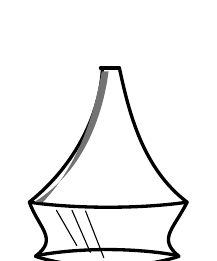
\begin{tikzpicture}[scale=0.86, line cap=round, line join=round]
  \draw[very thick] (-0.10,2.80) -- (0.18,2.80);
  \draw[very thick] (-0.07,2.80) .. controls (-0.10,2.15) and (-0.45,1.38) .. (-1.15,0.82);
  \draw[very thick] (0.18,2.80) .. controls (0.32,2.15) and (0.52,1.32) .. (1.18,0.82);
  \draw[very thick] (-1.15,0.82) .. controls (-1.00,0.42) and (-0.72,0.28) .. (-1.06,0.02);
  \draw[very thick] (1.18,0.82) .. controls (0.98,0.42) and (0.74,0.28) .. (1.06,0.02);
  \draw[very thick] (-1.06,0.02) .. controls (-0.45,-0.18) and (0.45,-0.18) .. (1.06,0.02);
  \draw[very thick] (-1.15,0.82) .. controls (-0.48,0.72) and (0.50,0.72) .. (1.18,0.82);
  \draw[very thick] (-1.05,0.03) .. controls (-0.42,0.15) and (0.42,0.15) .. (1.05,0.03);
  \fill[black!55] (-0.95,0.82) .. controls (-0.38,1.42) and (-0.18,2.20) .. (-0.08,2.75) -- (0.02,2.75) .. controls (-0.05,2.20) and (-0.30,1.30) .. (-1.08,0.82) -- cycle;
  \draw[thin] (-0.75,0.70)--(-0.45,0.18);
  \draw[thin] (-0.52,0.70)--(-0.25,0.08);
  \draw[thin] (-0.32,0.69)--(-0.05,0.00);
\end{tikzpicture}

{\footnotesize\bfseries Fig. 1.\({}^{\rm a}\) -- Pseudosfera.}
\end{center}

\emph{Caso II. Tipo ellittico.} Per ottenere una superficie reale bisogna supporre
\[
 \frac{\lambda}{R}<1
\]
e ponendo \(\lambda=R\sen\alpha\), il massimo valore per \(\cosh\dfrac{u}{R}\) sarà \(\dfrac1{\sen\alpha}\) e però il raggio \(r\) del parallelo oscilla fra
\[
 r=0
 \qquad\hbox{e}\qquad
 r=R\cos\alpha.
\]
Quando \(r=0\), è \(\dfrac{dr}{du}=\sen\alpha\) e però tutti i meridiani incontrano in \(u=0\) l'asse di rotazione sotto l'angolo \(\alpha\); questo punto è un punto conico della superficie.

Le coordinate di un punto della curva meridiana si esprimono per funzioni ellittiche di un parametro \(\tau\), col modulo \(k=\cos\alpha\). Poniamo infatti
\[
 \senh\frac{u}{R}=\frac{k}{k'}\cn(\tau,k)
\]
ed avremo
\[
 r=Rk\cn\tau,
 \qquad
 z=Rk'\int_0^\tau \sn^2\tau\,d\tau
 =R\left\{\frac{H}{K}\tau-Z(\tau)\right\},
\]
essendo
\[
 Z(\tau)=\frac{\Theta'(\tau)}{\Theta(\tau)}
\]
la funzione di Jacobi e H, K le note costanti della teoria delle funzioni ellittiche. Il tratto della curva da \(\tau=0\) a \(\tau=2K\) è rappresentato nella figura II); quando \(\tau\) aumenta di \(4K\) la curva si riproduce periodicamente. La superficie di rotazione corrispondente consta di infinite parti congruenti per traslazione lungo l'asse; i paralleli massimi di raggio \(r=R\cos\alpha\) sono di regresso per la superficie, poichè i punti \(\tau=2mK\) (\(m\) intero) sono cuspidi del meridiano.

\begin{center}
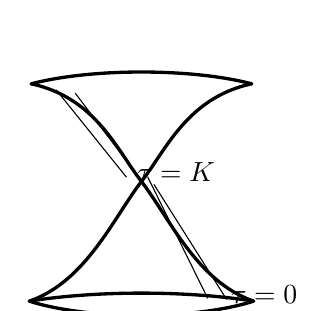
\begin{tikzpicture}[scale=0.8, line cap=round, line join=round]
  \draw[very thick] (-1.75,2.10) .. controls (-0.80,2.35) and (0.80,2.35) .. (1.75,2.10);
  \draw[very thick] (-1.75,2.10) .. controls (-0.72,1.88) and (-0.38,1.03) .. (0,0.55);
  \draw[very thick] (1.75,2.10) .. controls (0.72,1.88) and (0.38,1.03) .. (0,0.55);
  \draw[very thick] (0,0.55) .. controls (-0.44,-0.02) and (-0.88,-1.04) .. (-1.78,-1.35);
  \draw[very thick] (0,0.55) .. controls (0.44,-0.02) and (0.88,-1.04) .. (1.78,-1.35);
  \draw[very thick] (-1.78,-1.35) .. controls (-0.84,-1.65) and (0.84,-1.65) .. (1.78,-1.35);
  \draw[very thick] (-1.78,-1.35) .. controls (-0.72,-1.18) and (0.72,-1.18) .. (1.78,-1.35);
  \draw[thin] (-1.35,2.00)--(-0.24,0.62);
  \draw[thin] (-1.05,1.95)--(-0.12,0.72);
  \draw[thin] (1.35,-1.32)--(0.20,0.50);
  \draw[thin] (1.05,-1.30)--(0.10,0.62);
  \node at (0.55,0.70) {\(\tau=K\)};
  \node at (1.95,-1.25) {\(\tau=0\)};
\end{tikzpicture}

{\footnotesize\bfseries Fig. 2.\({}^{\rm a}\) -- Superficie pseudosferica di rotazione del tipo ellittico.}
\end{center}

\emph{Caso III. Tipo iperbolico.} In questo caso abbiamo
\[
 r=\lambda\cosh\frac{u}{R},
 \qquad
 \frac{dr}{du}=\frac{\lambda}{R}\senh\frac{u}{R};
\]
il massimo valore che assume \(u\) nel tratto reale della curva corrisponde a \(\senh\dfrac{u}{R}=\dfrac{R}{\lambda}\), e il raggio del parallelo oscilla fra il minimo \(\lambda\) e il massimo \(\sqrt{R^2+\lambda^2}\).

Ponendo qui
\[
 \frac{R}{\sqrt{R^2+\lambda^2}}=k,
 \qquad
 \cosh\frac{u}{R}=\frac{\dn(\tau,k)}{k},
\]
esprimeremo le coordinate di un punto mobile sulla curva per funzioni ellittiche del parametro \(\tau\) colle formole
\[
 r=\frac{R}{k}\dn\tau,
 \qquad
 z=\frac{R}{k}\left\{\frac{H}{K}\tau-Z(\tau)\right\}.
\]
La forma della curva da \(\tau=0\) a \(\tau=2K\) è rappresentata nella figura 3.\({}^{\rm a}\); quando \(\tau\) aumenta di \(2K\), la curva si riproduce periodicamente. I paralleli massimi corrispondenti a \(\tau=2mK\) (\(m\) intero) sono di regresso per la superficie e quelli minimi corrispondenti a \(\tau=(2m+1)K\) sono geodetiche.

\begin{center}
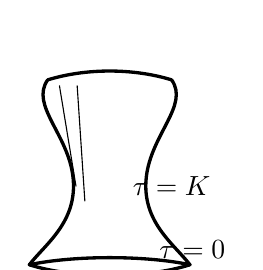
\begin{tikzpicture}[scale=0.75, line cap=round, line join=round]
  \draw[very thick] (-1.05,2.05) .. controls (-0.40,2.25) and (0.40,2.25) .. (1.05,2.05);
  \draw[very thick] (-1.05,2.05) .. controls (-1.35,1.62) and (-0.70,1.13) .. (-0.62,0.40)
                     .. controls (-0.54,-0.35) and (-1.08,-0.72) .. (-1.36,-1.08);
  \draw[very thick] (1.05,2.05) .. controls (1.35,1.62) and (0.70,1.13) .. (0.62,0.40)
                     .. controls (0.54,-0.35) and (1.08,-0.72) .. (1.36,-1.08);
  \draw[very thick] (-1.36,-1.08) .. controls (-0.62,-1.32) and (0.62,-1.32) .. (1.36,-1.08);
  \draw[very thick] (-1.36,-1.08) .. controls (-0.60,-0.92) and (0.60,-0.92) .. (1.36,-1.08);
  \draw[thin] (-0.85,1.95)--(-0.57,0.25);
  \draw[thin] (-0.55,1.95)--(-0.42,0.00);
  \node at (1.05,0.25) {\(\tau=K\)};
  \node at (1.40,-0.82) {\(\tau=0\)};
\end{tikzpicture}

{\footnotesize\bfseries Fig. 3.\({}^{\rm a}\) -- Superficie pseudosferica di rotazione del tipo iperbolico.}
\end{center}

Le tre forme di superficie pseudosferiche di rotazione ora considerate sono fra loro distinte, nè è possibile applicare una di esse sopra un'altra di specie diversa in guisa che i paralleli si distendano sui paralleli. Per accertarsene basta osservare che nel tipo parabolico i paralleli sono a curvatura geodetica costante \(\dfrac1R\), nel tipo ellittico la curvatura geodetica dei paralleli è \(>\dfrac1R\) e nel tipo iperbolico invece \(<\dfrac1R\). Però stante il teorema generale (§. 100), ogni superficie pseudosferica di raggio R è applicabile sopra ciascuna delle superficie I) II) III). Volendo considerare più da vicino questo modo di deformazione di ogni superficie pseudosferica a superficie di rotazione, faremo le osservazioni seguenti:

a) Sopra una superficie pseudosferica S si tracci un oriciclo e si considerino le geodetiche ad esso ortogonali. Per flessione potrà darsi alla superficie la forma di una pseudosfera, di cui le geodetiche segnate diventeranno i meridiani.

b) Sulla superficie pseudosferica S si segni un punto P e si considerino le geodetiche uscenti da P e i circoli geodetici ortogonali; assumendo i parametri \(u,v\) come a pag. 224, avremo
\[
 ds_1^2=du^2+R^2\senh^2\frac{u}{R}\,dv^2.
\]
Confrontando coll'elemento lineare della superficie di rotazione del tipo ellittico
\[
 ds_1^2=du_1^2+\lambda^2\senh^2\frac{u_1}{R}\,dv_1^2,
\]
otterremo per le formule d'applicabilità
\[
 u_1=u,
 \qquad
 \frac{\lambda}{R}v_1=v.
\]
Ne risulta che quando alla longitudine \(v_1\), nella superficie di rotazione II), si fa compiere un intero giro da 0 a \(2\pi\), l'angolo \(v\) percorre l'intervallo fra \(v=0\) e \(v=2\pi\sen\alpha<2\pi\). Basta dunque una porzione di S attorno a P per ricoprire interamente una falda della superficie II). Inoltre la parte di S al di là del circolo geodetico di raggio
\[
 u=\sett\cosh\left(\frac1{\sen\alpha}\right)
\]
non ha corrispondente sulla superficie (II); la porzione di S attorno a P, alla quale si può dare la forma di una falda della superficie II), è dunque limitata da un settore geodetico.

c) Nel caso delle superficie III) del tipo iperbolico il parallelo minimo è una geodetica e potremo quindi applicare una superficie pseudosferica qualunque S sopra la III) in modo che una geodetica arbitraria \(g\) di S si distenda sul parallelo minimo. La parte di S, che si applica effettivamente sopra una falda della III), è racchiusa da una striscia limitata da due linee geodeticamente parallele alla \(g\) ed equidistanti da essa, le quali dopo la deformazione diventano i paralleli massimi (di regresso) della zona. Nel senso della geodetica \(g\) la striscia è poi limitata da due geodetiche ortogonali a \(g\), le quali si riuniscono dopo la deformazione in un solo meridiano della zona. La lunghezza e la larghezza della striscia dipendono solo dal raggio che si vuol dare al parallelo minimo.

\subsection*{\S. 104.\quad Superficie con \(\infty^1\) applicabilità in sè stesso.}

La proprietà fondamentale delle superficie a curvatura costante, che abbiamo dimostrato al §. 100, può enunciarsi dicendo:

\emph{L'elemento lineare di ogni superficie a curvatura costante ammette \(\infty^3\) trasformazioni in sè medesimo.}

Domandiamo ora se esistono altre superficie che ammettono flessioni continue in sè medesime. Se queste flessioni costituissero una doppia infinità, ogni punto della superficie, disponendo dei due parametri della trasformazione, si potrebbe trasportare in qualunque altro punto (di una conveniente regione) e, pel teorema di Gauss, la superficie sarebbe a curvatura costante e le flessioni supposte costituirebbero una tripla anzichè una doppia infinità.

Ora è chiaro che ogni superficie applicabile sopra una superficie di rotazione ammette una flessione continua in sè medesima, corrispondente alla rotazione della superficie su cui è applicabile attorno all'asse.

Importa osservare che sussiste il teorema inverso:

\emph{Ogni superficie S, che ammette una flessione continua in sè medesima, è applicabile sopra una superficie di rotazione.} In sostanza questo teorema risulta già dalla discussione al §. 99, poichè ivi si è visto come le formole d'applicabilità di due superficie S, S' possono contenere un parametro arbitrario nel solo caso che le S, S' siano applicabili sulla stessa superficie di rotazione. Ma possiamo dimostrare nuovamente la proprietà colle considerazioni geometriche seguenti. Se la S è a curvatura costante, il teorema è già provato dalle ricerche dei numeri precedenti. In caso contrario, durante la flessione continua supposta, le linee L di egual curvatura
\[
 K=\hbox{costante}
\]
dovranno, pel teorema di Gauss, strisciare sopra sè medesime. E poichè tale flessione dipende da un parametro variabile con continuità, ogni punto di una linea L può trasportarsi in qualunque altro punto della linea stessa; ne risulta che le linee L sono a curvatura geodetica costante. Inoltre le linee geodeticamente parallele ad una linea L, durante la detta flessione, strisciano pure evidentemente sopra sè medesime. Da queste considerazioni segue facilmente il teorema enunciato, e invero sussiste la proprietà:

\emph{Se una superficie S possiede un sistema di linee L geodeticamente parallele e a curvatura geodetica costante, essa è applicabile sopra una superficie di rotazione, i cui paralleli sono le deformate delle linee L.}

Prendasi infatti a sistema coordinato quello formato dalle linee L (\(u=\) costante) e dalle geodetiche ortogonali (\(v=\) costante); l'elemento lineare prenderà la forma
\[
 ds^2=du^2+G\,dv^2.
\]
Ora è per ipotesi
\[
 -\frac1{\rho_u}=\frac{\partial\log\sqrt G}{\partial u}=\varphi(u),
\]
onde
\[
 \sqrt G=UV,
\]
essendo U funzione di \(u\) e V di \(v\). Ponendo
\[
 \int V\,dv=v_1,
\]
si pone in evidenza l'elemento lineare
\[
 ds^2=du^2+U^2\,dv_1^2
\]
di una superficie di rotazione.

\subsection*{\S. 105.\quad Superficie di rotazione applicabili.}

Consideriamo ora alcuni semplici esempî di superficie applicabili e in primo luogo cerchiamo se due superficie di rotazione S, S\(_1\) possono essere applicabili l'una sull'altra.

Dal teorema di Gauss segue anzitutto che i paralleli di S si distenderanno sui paralleli di S\(_1\), e quindi anche i meridiani sui meridiani. Naturalmente fanno eccezione le superficie a curvatura costante, ma le considerazioni seguenti valgono anche per queste superficie, quando si aggiunga la condizione che i paralleli dell'una si distendano sui paralleli dell'altra.

Se l'elemento lineare di S è dato da
\[
 ds^2=du^2+r^2\,dv^2
\]
e quello di S\(_1\) da
\[
 ds_1^2=du_1^2+r_1^2\,dv_1^2,
\]
potremo fare senz'altro \(u_1=u\), contando gli archi meridiani da due paralleli corrispondenti. Per trasformare i due elementi lineari l'uno nell'altro, converrà porre \(v_1=v_1(v)\), determinando questa funzione dalla condizione
\[
 r_1(u)\frac{dv_1}{dv}=r(u).
\]
Di qui risulta
\[
 r_1=kr,
 \qquad
 v_1=\frac{v}{k}\quad (k\hbox{ costante arbitraria}).
\]
Se adunque \(r=\varphi(u)\) è l'equazione del meridiano di S, le coordinate del meridiano di S\(_1\) saranno date da
\[
 r=k\varphi(u),
 \qquad
 z=\int\sqrt{1-k^2\varphi'^2(u)}\,du.
\]
Ne segue: \emph{Ogni superficie di rotazione può deformarsi in \(\infty^1\) modi, conservandosi superficie di rotazione.}

Consideriamo più da vicino il modo d'applicarsi della S\(_1\) sulla S. Se supponiamo \(k<1\), la formula
\[
 v=kv_1
\]
dimostra che quando la longitudine \(v_1\) ha compiuto un intero giro su S\(_1\) diventando eguale a \(2\pi\), la longitudine \(v\) diventa
\[
 v=2k\pi<2\pi.
\]
Dunque, applicando la S\(_1\) sulla S, questa non ne resta interamente coperta, ma viene a mancarne una porzione (fuso) compreso fra due meridiani, i cui piani formano un angolo di ampiezza eguale a \(2\pi(1-k)\). Per distendere S\(_1\) sopra S, conviene quindi tagliare S\(_1\) lungo un meridiano ed aprirla deformandola in guisa che gli orli del taglio diventino sopra S due meridiani distinti. Se si osserva che la curvatura geodetica dei paralleli e la curvatura totale della superficie non variano nella deformazione, si vedrà subito che in due punti corrispondenti la curvatura del meridiano di S supera quella del meridiano di S\(_1\).

Al caso \(k>1\) corrisponde evidentemente la deformazione inversa di S in S\(_1\), per la quale conviene togliere da S un fuso, ristabilendo poi la continuità della superficie col riunire per deformazione in un solo i due meridiani del fuso tolto. È poi da osservare che ad un punto del meridiano di S corrisponde un punto reale del meridiano di S\(_1\) finchè \(k\dfrac{dr}{du}<1\), ciò che sempre avviene se \(k<1\). Ma quando \(k>1\) i paralleli, cui corrisponde il valore \(\dfrac1k\) di \(\dfrac{dr}{du}\), limitano sopra S una zona, che è la porzione di S effettivamente applicabile sopra S\(_1\). Dopo la deformazione, i paralleli estremi di questa zona diventano paralleli di regresso per S\(_1\).

Come esempio, consideriamo le deformazioni delle superficie di rotazione a curvatura costante.

a) Per la sfera di raggio \emph{uno} si può assumere.
\[
 r=\cos u
\]
e le coordinate dei meridiani deformati sono date dalle formole
\[
 r=k\cos u,
 \qquad
 z=\int\sqrt{1-k^2\sen^2 u}\,du.
\]
Possiamo esprimerle per funzioni ellittiche di un parametro \(\tau\). Perciò, se \(k<1\), poniamo \(\cos u=\cn(\tau,k)\) e avremo
\[
 r=k\cn\tau,
 \qquad
 z=\left(1-\frac{H}{K}\right)\tau+Z(\tau);
\]
se \(k>1\) cangiamo \(k\) in \(\dfrac1k\) e ponendo
\[
 \cos u=\dn(\tau,k)
\]
avremo
\[
 r=\frac{\dn\tau}{k},
 \qquad
 z=\left(k-\frac{H}{Kk}\right)\tau+\frac1k Z(\tau).
\]
Nel caso di \(k<1\), si otterrà una superficie a forma di fuso, i cui meridiani incontrano l'asse in un punto (conico per la superficie) sotto l'angolo \(\alpha=\arc\sen k\). Nel caso \(k>1\) si ha una zona limitata a due paralleli minimi di regresso. Le tre figure seguenti rappresentano appunto le superficie corrispondenti ai tre casi. Sulla intermedia, sfera, è segnata la zona che si applica sulla superficie della fig. 6.\({}^{\rm a}\)

\begin{center}
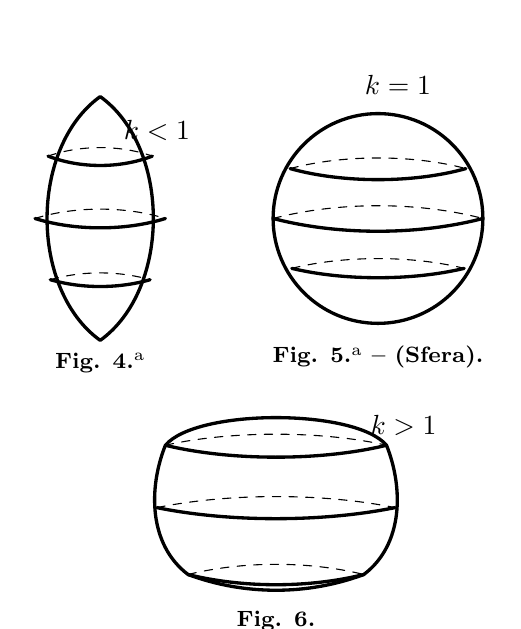
\begin{tikzpicture}[scale=0.72, line cap=round, line join=round]
  \begin{scope}[xshift=-3.7cm]
    \draw[very thick] (0,2.15) .. controls (-1.25,1.25) and (-1.25,-1.25) .. (0,-2.15)
                      .. controls (1.25,-1.25) and (1.25,1.25) .. (0,2.15);
    \draw[very thick] (-0.92,1.10) .. controls (-0.35,0.88) and (0.35,0.88) .. (0.92,1.10);
    \draw[dashed] (-0.92,1.10) .. controls (-0.35,1.30) and (0.35,1.30) .. (0.92,1.10);
    \draw[very thick] (-1.15,0.00) .. controls (-0.45,-0.22) and (0.45,-0.22) .. (1.15,0.00);
    \draw[dashed] (-1.15,0.00) .. controls (-0.45,0.22) and (0.45,0.22) .. (1.15,0.00);
    \draw[very thick] (-0.88,-1.08) .. controls (-0.32,-1.24) and (0.32,-1.24) .. (0.88,-1.08);
    \draw[dashed] (-0.88,-1.08) .. controls (-0.32,-0.92) and (0.32,-0.92) .. (0.88,-1.08);
    \node at (1.00,1.55) {\(k<1\)};
    \node at (0,-2.55) {\footnotesize\bfseries Fig. 4.\({}^{\rm a}\)};
  \end{scope}
  \begin{scope}[xshift=1.2cm]
    \draw[very thick] (0,0) circle (1.85);
    \draw[very thick] (-1.55,0.88) .. controls (-0.62,0.62) and (0.62,0.62) .. (1.55,0.88);
    \draw[dashed] (-1.55,0.88) .. controls (-0.62,1.13) and (0.62,1.13) .. (1.55,0.88);
    \draw[very thick] (-1.85,0.0) .. controls (-0.70,-0.30) and (0.70,-0.30) .. (1.85,0.0);
    \draw[dashed] (-1.85,0.0) .. controls (-0.70,0.30) and (0.70,0.30) .. (1.85,0.0);
    \draw[very thick] (-1.52,-0.88) .. controls (-0.60,-1.10) and (0.60,-1.10) .. (1.52,-0.88);
    \draw[dashed] (-1.52,-0.88) .. controls (-0.60,-0.65) and (0.60,-0.65) .. (1.52,-0.88);
    \node at (0.35,2.35) {\(k=1\)};
    \node at (0,-2.45) {\footnotesize\bfseries Fig. 5.\({}^{\rm a}\) -- (Sfera).};
  \end{scope}
  \begin{scope}[xshift=-0.6cm,yshift=-5.1cm]
    \draw[very thick] (-1.95,1.10) .. controls (-1.40,1.75) and (1.40,1.75) .. (1.95,1.10)
                      .. controls (2.25,0.35) and (2.25,-0.65) .. (1.55,-1.18)
                      .. controls (0.55,-1.55) and (-0.55,-1.55) .. (-1.55,-1.18)
                      .. controls (-2.25,-0.65) and (-2.25,0.35) .. (-1.95,1.10);
    \draw[very thick] (-1.95,1.10) .. controls (-0.80,0.82) and (0.80,0.82) .. (1.95,1.10);
    \draw[dashed] (-1.95,1.10) .. controls (-0.80,1.36) and (0.80,1.36) .. (1.95,1.10);
    \draw[very thick] (-2.10,0.00) .. controls (-0.82,-0.26) and (0.82,-0.26) .. (2.10,0.00);
    \draw[dashed] (-2.10,0.00) .. controls (-0.82,0.26) and (0.82,0.26) .. (2.10,0.00);
    \draw[very thick] (-1.55,-1.18) .. controls (-0.58,-1.42) and (0.58,-1.42) .. (1.55,-1.18);
    \draw[dashed] (-1.55,-1.18) .. controls (-0.58,-0.94) and (0.58,-0.94) .. (1.55,-1.18);
    \node at (2.25,1.45) {\(k>1\)};
    \node at (0,-2.00) {\footnotesize\bfseries Fig. 6.};
  \end{scope}
\end{tikzpicture}
\end{center}

b) La pseudosfera gode della singolare proprietà che tutte le sue deformate di rotazione coincidono colla pseudosfera stessa, come risulta dall'osservazione che la curvatura geodetica dei paralleli è costante \(=\dfrac1R\).

Nel caso del restringimento dei paralleli (\(k<1\)) il parallelo massimo (di regresso) diventa un parallelo minore e resta così scoperta la zona compresa fra questo parallelo e quello massimo. Nella deformazione inversa un parallelo minore diventa il parallelo di regresso; ma per effettuare questa deformazione occorre prima tagliare dalla pseudosfera la zona compresa fra questo parallelo e il parallelo attuale di regresso.

La deformazione delle altre due classi di superficie pseudosferiche di rotazione conduce a superficie del medesimo tipo, variando nel caso delle superficie del tipo ellittico l'angolo d'apertura al vertice (punto conico) e per quelle del tipo iperbolico il raggio del parallelo minimo.

\subsection*{\S. 106.\quad Elicoidi e teorema di Bour.}

Il risultato del §. 104 consente un'immediata applicazione ad una importante classe di superficie, che diconsi \emph{elicoidi}. Sono queste le superficie generate da una curva piana o a doppia curvatura, dotata attorno ad un asse e parallelamente a questo di un doppio movimento rotatorio e traslatorio, il rapporto delle cui velocità sia costante. I vari punti della curva generatrice descrivono altrettante eliche circolari, aventi per asse comune l'asse dell'elicoide e tutte del medesimo passo. Se osserviamo che il moto elicoidale, col quale la superficie è stata generata, fa strisciare l'intiera superficie sopra sè medesima, basterà applicare il teorema del §. 105 per ottenere l'elegante risultato dovuto a Bour:

\emph{Ogni elicoide è applicabile sopra una superficie di rotazione; le eliche si distendono sui paralleli.}

È chiaro che la superficie di rotazione è ricoperta infinite volte dall'elicoide, ogni elica avvolgendo infinite volte il corrispondente parallelo.

Diamo ora una dimostrazione diretta di questo teorema, per trovare altresì le effettive formole dell'applicabilità. Osserviamo per ciò che conducendo un piano per l'asse si produce nell'elicoide una sezione, e se a questa sezione (\emph{profilo meridiano}) si dà attorno all'asse il moto elicoidale che ha generato la superficie, la sezione stessa descriverà l'elicoide. Un'elicoide è individuata, se viene assegnato il suo profilo meridiano e il parametro del moto elicoidale.

Preso per asse delle \(z\) l'asse dell'elicoide, e indicando con \(\rho\) la distanza di un punto del profilo meridiano dall'asse, sia
\[
 z=\varphi(\rho)
\]
l'equazione del profilo meridiano. Indichiamo poi con \(v\) l'angolo di cui ha rotato, dopo un tempo qualunque, il piano del profilo meridiano e con \(m\)
il rapporto della velocità di traslazione a quella di rotazione. Le coordinate \(x,y,z\) di un punto mobile sull'elicoide saranno date in funzione di \(\rho,v\) dalle formole
\[
 x=\rho\cos v,
 \qquad y=\rho\sen v,
 \qquad z=\varphi(\rho)+mv,
\]
da cui
\[
 ds^2=\{1+\varphi'^2(\rho)\}\,d\rho^2+2m\varphi'(\rho)\,d\rho\,dv+(\rho^2+m^2)\,dv^2.
\]
Cangiamo le linee coordinate \(v\), ponendo
\[
 v=kv_1-m\int\frac{\varphi'(\rho)\,d\rho}{\rho^2+m^2},
\]
essendo \(k\) una costante arbitraria, e ne risulterà
\[
 ds^2=\left\{1+\frac{\rho^2\varphi'^2(\rho)}{\rho^2+m^2}\right\}d\rho^2+k^2(\rho^2+m^2)\,dv_1^2.
\]
Paragonando questo elemento lineare con quello
\[
 ds_1^2=\{1+\psi'^2(r)\}\,dr^2+r^2dv_1^2
\]
di una superficie di rotazione, di cui
\[
 z=\psi(r)
\]
sia l'equazione della curva meridiana, li potremo identificare, ponendo fra \(r,\psi(r),\rho,\varphi(\rho)\) le relazioni
\begin{equation}\tag{8}
\left\{
\begin{aligned}
 r^2&=k^2(\rho^2+m^2),\\
 \{1+\psi'^2(r)\}\left(\frac{dr}{d\rho}\right)^2
 &=1+\frac{\rho^2\varphi'^2(\rho)}{\rho^2+m^2}.
\end{aligned}
\right.
\end{equation}
Queste formole dimostrano di nuovo il teorema di Bour; di più si vede che presa ad arbitrio un'elicoide o una superficie di rotazione, si potranno trovare con quadrature le superficie di rotazione o le elicoidi su cui sono applicabili. Nel primo caso, eliminando \(\rho\), si avrà infatti \(\psi'(r)\) e nel secondo, eliminando \(r\), si otterrà \(\varphi'(\rho)\).

\subsection*{\S. 107.\quad Elicoide rigata d'area minima ed iperboloide rigato.}

Applichiamo le formole (8) a due semplici esempî.

\(1.^\circ\) Il profilo meridiano sia una retta perpendicolare all'asse; l'elicoide generata è \emph{l'elicoide rigata d'area minima} già considerata al \S. 24 c. I. Avremo allora nelle (8) \(\varphi'(\rho)=0\), quindi
\[
 1+\psi'^2(r)=\left(\frac{d\rho}{dr}\right)^2=\frac{r^2}{k^2(r^2-m^2k^2)}
\]
e prendendo la costante arbitraria \(k=1\), risulterà
\[
 z=\psi(r)=m\int\frac{dr}{\sqrt{r^2-m^2}}
\]
ed eseguendo la quadratura
\[
 r=m\cosh\frac{z}{m}.
\]
La curva meridiana è adunque una catenaria comune, avente per direttrice l'asse di rotazione.

La superficie di rotazione corrispondente dicesi \emph{catenoide}. Le generatrici dell'elicoide si distendono sui meridiani e l'asse \(\rho=0\) diventa il circolo di gola \(r=m\) del catenoide.

\(2.^\circ\) Il profilo meridiano sia una retta inclinata sull'asse di un angolo \(\alpha\); la sua equazione sarà
\[
 z=\rho\cot\alpha
\]
e ponendo nelle (8)
\[
 \varphi'(\rho)=\cot\alpha,
\]
risulterà
\[
 1+\psi'^2(r)=\left\{1+\frac{(r^2-k^2m^2)\cot^2\alpha}{r^2}\right\}
 \frac{r^2}{k^2(r^2-k^2m^2)}
\]
e ponendo
\[
 k=\cot\alpha,
\]
avremo
\[
 \psi'(r)=\frac{\tg\alpha\,r}{\sqrt{r^2-m^2\cot^2\alpha}}.
\]
L'equazione del meridiano della superficie di rotazione è adunque
\[
 z=\tg\alpha\sqrt{r^2-m^2\cot^2\alpha},
\]
cioè
\[
 \frac{r^2}{m^2\cot^2\alpha}-\frac{z^2}{m^2}=1.
\]
La superficie di rotazione è quindi un iperboloide di rotazione ad una falda. Facilmente si vede che l'asse \(\rho=0\) dell'elicoide si distende sul circolo di gola dell'iperboloide e le generatrici dell'elicoide sulle generatrici di un sistema dell'iperboloide.

\subsection*{\S. 108.\quad Il secondo problema dell'applicabilità.}

Passiamo ora a trattare del secondo e più importante problema della teoria dell'applicabilità, che consisterebbe nel: \emph{Trovare tutte le superficie applicabili sopra una superficie data}, ovvero: \emph{Trovare tutte le superficie con assegnato elemento lineare}.

Questo difficile problema non si sa risolvere completamente che in pochi casi particolari, che verranno considerati nel seguito di questo trattato. Però i teoremi generali sulle equazioni a derivate parziali permettono di stabilire dei risultati generali molto importanti relativi al problema enunciato. E di questi appunto vogliamo ora occuparci, per quanto lo consentono i limiti di brevità che ci siamo imposti\srcfn{1}{Il lettore troverà nel tomo III delle lezioni di Darboux p. 263 ss. una trattazione completa del problema.}.

Un primo modo di trattare il problema attuale risulta naturalmente dalle formole fondamentali della teoria delle superficie (cap. IV). Essendo assegnata la prima forma fondamentale
\[
 E\,du^2+2F\,du\,dv+G\,dv^2,
\]
ad ogni superficie col dato elemento lineare corrisponderà una seconda forma fondamentale
\[
 D\,du^2+2D'\,du\,dv+D''\,dv^2,
\]
e le funzioni \(D,D',D''\) dovranno soddisfare alle equazioni (III), (IV) \S. 56 (pag. 119), cioè alla equazione di Gauss e alle due equazioni di Codazzi. Viceversa, se \(D,D',D''\) sono tre funzioni di \(u,v\) che soddisfano alle tre citate equazioni, esiste una superficie corrispondente coll'elemento lineare assegnato, e la sua effettiva ricerca dipende ulteriormente da un'equazione di Riccati.

Così p. e. se prendessimo l'elemento lineare di una superficie di rotazione
\[
 ds^2=du^2+r^2dv^2,
\]
potremmo soddisfare alle citate equazioni fondamentali prendendo \(D,D',D''\) funzioni della sola \(u\). Le superficie applicabili sulle superficie di rotazione, che così troveremmo, sarebbero appunto le elicoidi \S. 106\srcfn{1}{Per dimostrarlo basta osservare che in questo caso tanto la prima quanto la seconda forma fondamentale ammettono la trasformazione continua in sè medesime:
\[
 u'=u,\qquad v'=v+\hbox{costante}
\]
e perciò la superficie, ammettendo un movimento continuo in sè medesima, è un'elicoide.}.

\subsection*{\S. 109.\quad Equazione a derivate parziali pel secondo problema.}

Ben più importante del metodo precedente è quello che ora passiamo ad esporre, fondandoci sul risultato ottenuto al \S. 69, e precisamente sulla equazione (B), pag. 146.

Per ogni superficie
\[
 x=x(u,v),\qquad y=y(u,v),\qquad z=z(u,v)
\]
coll'assegnato elemento lineare
\begin{equation}\tag{9}
 dx^2+dy^2+dz^2=E\,du^2+2F\,du\,dv+G\,dv^2
\end{equation}
l'equazione ora ricordata insegna che ciascuna delle tre funzioni incognite \(x,y,z\) soddisfa alla equazione a derivate parziali del \(2.^\circ\) ordine
\begin{equation}\tag{10}
 \Delta_{22}x=(1-\Delta_1x)K,
\end{equation}
i cui coefficienti sono appunto formati con \(E,F,G\) e le loro derivate prime e seconde\srcfn{2}{Se, usando delle notazioni di Monge, si indicano con \(p,q;r,s,t\) le derivate prime e seconde della funzione incognita, l'equazione si scrive
\[
\begin{aligned}
&\left(r-\chr{1}{1}{1}p-\chr{1}{1}{2}q\right)
 \left(t-\chr{2}{2}{1}p-\chr{2}{2}{2}q\right)
-\left(s-\chr{1}{2}{1}p-\chr{1}{2}{2}q\right)^2 \\
&\hspace{3em}=K\left\{EG-F^2-\left[E q^2-2Fpq+G p^2\right]\right\}
\end{aligned}
\]
ed ha la forma lineare di Ampère rapporto a \(rt-s^2\), \(r,s,t\).}.

Ora importa osservare con Darboux che l'equazione (10) ha il significato seguente:
\begin{center}
\emph{Se \(x(u,v)\) ne è una soluzione, la forma quadratica}
\end{center}
\[
\begin{aligned}
&E\,du^2+2F\,du\,dv+G\,dv^2-dx^2 \\
&=\left\{E-\left(\frac{\partial x}{\partial u}\right)^2\right\}du^2
+2\left\{F-\frac{\partial x}{\partial u}\frac{\partial x}{\partial v}\right\}du\,dv
+\left\{G-\left(\frac{\partial x}{\partial v}\right)^2\right\}dv^2
\end{aligned}
\]
\begin{center}
\emph{avrà la curvatura nulla.}
\end{center}
Per dimostrarlo nel modo più semplice si faccia
\[
 x=u,
 \qquad F=0,
\]
il che evidentemente è lecito per la proprietà invariantiva della nostra equazione. La (10) diventa allora
\[
 \chr{1}{1}{1}\chr{2}{2}{1}-\chr{1}{2}{1}^2=G(E-1)K
\]
e, sostituendo ai simboli di Christoffel i loro attuali valori
\[
 \chr{1}{1}{1}=\frac1{2E}\frac{\partial E}{\partial u},\qquad
 \chr{1}{2}{1}=\frac1{2E}\frac{\partial E}{\partial v},\qquad
 \chr{2}{2}{1}=-\frac1{2E}\frac{\partial G}{\partial u},
\]
si ottiene
\[
 \frac{\partial E}{\partial u}\frac{\partial G}{\partial u}
 +\left(\frac{\partial E}{\partial v}\right)^2
 +4E^2G(E-1)K=0.
\]
Ora in coordinate ortogonali si ha (\S. 43, pag. 93):
\begin{equation}\tag{11}
\begin{aligned}
4E^2G^2K={}&E\left[\frac{\partial E}{\partial v}\frac{\partial G}{\partial v}+
\left(\frac{\partial G}{\partial u}\right)^2\right]
+G\left[\frac{\partial E}{\partial u}\frac{\partial G}{\partial u}+
\left(\frac{\partial E}{\partial v}\right)^2\right]\\
&-2EG\left[\frac{\partial^2E}{\partial v^2}+\frac{\partial^2G}{\partial u^2}\right]
\end{aligned}
\end{equation}
e la precedente, moltiplicata per \(G\), si scrive
\[
\begin{aligned}
&G\left[\frac{\partial E}{\partial u}\frac{\partial G}{\partial u}+
\left(\frac{\partial E}{\partial v}\right)^2\right]
+E(E-1)\left[\frac{\partial E}{\partial v}\frac{\partial G}{\partial v}+
\left(\frac{\partial G}{\partial u}\right)^2\right] \\
&\quad+G(E-1)\left[\frac{\partial E}{\partial u}\frac{\partial G}{\partial u}+
\left(\frac{\partial E}{\partial v}\right)^2\right]
-2EG(E-1)\left(\frac{\partial^2E}{\partial v^2}+\frac{\partial^2G}{\partial u^2}\right)=0.
\end{aligned}
\]
Sopprimendo i termini che si distruggono e dividendo per \(E\), si ottiene l'equazione equivalente
\[
\begin{aligned}
&(E-1)\left[\frac{\partial E}{\partial v}\frac{\partial G}{\partial v}+
\left(\frac{\partial G}{\partial u}\right)^2\right]
+G\left[\frac{\partial G}{\partial u}\frac{\partial E}{\partial u}+
\left(\frac{\partial E}{\partial v}\right)^2\right]\\
&\qquad -2(E-1)G\left[\frac{\partial^2E}{\partial v^2}+\frac{\partial^2G}{\partial u^2}\right]=0,
\end{aligned}
\]
la quale, secondo la (11) stessa, esprime appunto che la forma
\[
 (E-1)du^2+Gdv^2
\]
ha la curvatura nulla.

Ciò premesso, supponiamo di conoscere una soluzione \(x(u,v)\) dell'equazione (10) e vediamo se esisterà una superficie reale corrispondente coll'assegnato elemento lineare. La forma differenziale
\begin{equation}\tag{12}
 E\,du^2+2F\,du\,dv+G\,dv^2-dx^2
\end{equation}
essendo allora a curvatura nulla, perchè esistano due altre funzioni reali \(y(u,v),z(u,v)\), che soddisfino la (9), è necessario e sufficiente che la (12) sia una forma definita, cioè si abbia
\[
\left[E-\left(\frac{\partial x}{\partial u}\right)^2\right]
\left[G-\left(\frac{\partial x}{\partial v}\right)^2\right]
-\left[F-\frac{\partial x}{\partial u}\frac{\partial x}{\partial v}\right]^2>0,
\]
ovvero
\[
 \Delta_1x<1.
\]
Supponendo questa condizione soddisfatta, si avranno \(y,z\) per quadrature (\S\S. 37 e 93); e manifestamente \(y,z\) saranno determinate a meno di una trasformazione di coordinate.

Dunque: \emph{Ad ogni soluzione reale \(x(u,v)\) dell'equazione (10), che soddisfi inoltre alla diseguaglianza \(\Delta_1x<1\), corrisponde una ed una sola superficie reale coll'assegnato elemento lineare. Nota la detta soluzione, la corrispondente superficie si avrà per quadrature.}

\subsection*{\S. 110.\quad Indeformabilità delle superficie con una linea rigida.}

Occupiamoci ora della questione seguente: \emph{Essendo data una superficie S e una curva \(\Gamma\) tracciata sopra di essa, può flettersi la superficie, senza deformare la curva?}

Nell'ipotesi affermativa, sia \(S_1\) una delle forme che assume S per flessione, restando rigida \(\Gamma\): potremo supporre la configurazione \(S_1\) della S così vicina alla iniziale che le normali ad \(S_1\), S lungo \(\Gamma\) siano vicine fra loro quanto si vuole. Ma allora, se si osserva che \(\Gamma\) avrà la medesima curvatura geodetica sopra \(S_1\) e S, e si ricorda la relazione che lega la curvatura geodetica coll'assoluta (\S. 84), si concluderà subito che lungo \(\Gamma\) le normali ad \(S_1\), S coincideranno.

Ora prendiamo per semplicità su S (e \(S_1\)) un sistema coordinato ortogonale \((u,v)\), e sia
\[
 v=0
\]
l'equazione della curva \(\Gamma\). Indichiamo coll'apposizione dell'indice 1 le quantità relative alla \(S_1\), ed avremo evidentemente:
\[
\left.
\begin{gathered}
 x_1=x,
 \quad y_1=y,
 \quad z_1=z,\\
 \frac{\partial x_1}{\partial u}=\frac{\partial x}{\partial u},\quad
 \frac{\partial y_1}{\partial u}=\frac{\partial y}{\partial u},\quad
 \frac{\partial z_1}{\partial u}=\frac{\partial z}{\partial u},\\
 \frac{\partial x_1}{\partial v}=\frac{\partial x}{\partial v},\quad
 \frac{\partial y_1}{\partial v}=\frac{\partial y}{\partial v},\quad
 \frac{\partial z_1}{\partial v}=\frac{\partial z}{\partial v},\\
 X_1=X,
 \quad Y_1=Y,
 \quad Z_1=Z
\end{gathered}
\right\}\quad \hbox{per }v=0.
\]
Ora, se consideriamo p. e. \(x_1,x\), esse sono soluzioni della medesima equazione a derivate parziali del secondo ordine (10), che coincidono nei loro valori e in quelle delle loro derivate prime per \(v=0\). Se proviamo che \emph{anche le tre derivate seconde di \(x_1\) coincidono con quelle corrispondenti di \(x\) per \(v=0\)}, in ordine ai teoremi generali sulle soluzioni delle equazioni a derivate parziali\srcfn{1}{Cf. p. e. \textsc{Goursat}. -- \emph{Leçons sur l'intégration des équations aux dérivées partielles du premier ordre}, p.\textsuperscript{e} 22.}, sarà dimostrato che \(x_1,x\) coincidono per tutti i valori di \(u,v\). Lo stesso potendosi ripetere per \(y_1,y;z_1,z\), ne seguirà che \(S_1,S\) coincidono. Ora dalle condizioni iniziali
\[
 \frac{\partial x_1}{\partial u}=\frac{\partial x}{\partial u},
 \qquad
 \frac{\partial x_1}{\partial v}=\frac{\partial x}{\partial v},
 \quad \hbox{per }v=0
\]
segue intanto
\[
 \frac{\partial^2x_1}{\partial u^2}=\frac{\partial^2x}{\partial u^2},
 \qquad
 \frac{\partial^2x_1}{\partial u\partial v}=\frac{\partial^2x}{\partial u\partial v},
 \quad \hbox{per }v=0.
\]
Le formole fondamentali (I) \S. 55, pag. 116, della teoria delle superficie dimostrano in conseguenza che si ha
\[
 D_1=D,
 \qquad D'_1=D',
 \quad \hbox{per }v=0.
\]
L'eguaglianza
\[
 DD''-D'^2=D_1D''_1-D_1'^2,
\]
fattovi \(v=0\), dà quindi
\[
 DD''=DD''_1,
 \quad \hbox{per }v=0.
\]
Ne segue
\[
 (D''_1)_{v=0}=(D'')_{v=0},
\]
\emph{a meno che non sia} \((D)_{v=0}=0\). Escluso questo caso, dalla terza delle citate formole (I) \S. 55 segue appunto, come si voleva provare
\[
 \frac{\partial^2x_1}{\partial v^2}=\frac{\partial^2x}{\partial v^2},
 \quad \hbox{per }v=0,
\]
e però \(S_1,S\) coincidono.

Nel caso escluso, \((D)_{v=0}=0\), la linea \(v=0\) è una linea assintotica di S; possiamo dunque enunciare il teorema: \emph{Se di una superficie flessibile S si mantiene rigida una curva \(\Gamma\), la superficie non si può deformare, a meno che la curva \(\Gamma\) non sia una linea assintotica di S.}

Nel caso che la linea \(\Gamma\) sia una linea assintotica, ulteriori proprietà delle equazioni a derivate parziali, le quali qui non possono che venire accennate, dimostrano che è effettivamente possibile deformare la superficie senza deformare la curva. È questa una singolare proprietà delle linee assintotiche, per la quale esse diconsi anche \emph{linee di piegamento}. Questa proprietà, che le distingue da ogni altra linea della superficie, dipende propriamente da ciò che: Sopra ogni superficie S le linee assintotiche sono le \emph{caratteristiche} dell'equazione a derivate parziali (10), da cui dipende la deformazione di S\srcfn{1}{Scritta la (10) sotto la forma
\[
 \Phi(r,s,t)=0
\]
della nota al numero precedente, l'equazione differenziale delle caratteristiche
\[
 \frac{\partial\Phi}{\partial t}\,du^2-\frac{\partial\Phi}{\partial s}\,du\,dv+\frac{\partial\Phi}{\partial r}\,dv^2=0,
\]
per le (I) \S. 55, diventa appunto l'equazione differenziale delle assintotiche
\[
 D\,du^2+2D'\,du\,dv+D''\,dv^2=0
\]
(Cf. \textsc{Darboux}, t. III, pag. 252).}.

\subsection*{\S. 111.\quad Deformazione della superficie con assegnata deformata di una curva.}

Il teorema ora dimostrato rende naturale la domanda: \emph{È possibile deformare una superficie \(S'\) in guisa che una curva assegnata C sopra di essa assuma una forma prestabilita \(\Gamma\)?}

Osserviamo in primo luogo che, se la deformazione cercata è possibile, la curvatura assoluta di \(\Gamma\) dovrà in ogni punto essere maggiore, o tutto al più eguale, alla curvatura geodetica di C nel punto corrispondente. Supponiamo questa condizione soddisfatta, ed anzi intendiamo per ora escluso il caso dell'eguaglianza della curvatura assoluta e geodetica di \(\Gamma\), chè allora la \(\Gamma\) sarebbe assintotica sulla superficie deformata.

Nell'ipotesi che esista la deformazione richiesta, sia S la superficie deformata, sulla quale prenderemo un sistema coordinato ortogonale \((u,v)\) come al numero precedente, tale che la curva \(\Gamma\) sia la \(v=0\). Fissiamo inoltre per maggior chiarezza che il parametro \(u\) sia l'arco di \(\Gamma\) contato da un suo punto fisso, talchè avremo
\[
 E=1,
 \quad \hbox{per }v=0.
\]
Indichiamo con \(\sigma\) l'angolo di cui deve rotare, in verso positivo, nel piano normale a \(\Gamma\), la direzione positiva della normale a S per sovrapporsi a quella della normale principale di \(\Gamma\). Ritenendo per la curva \(\Gamma\) le solite notazioni della teoria delle curve (c. I), avremo così, per \(v=0\):
\begin{equation}\tag{13}
\left\{
\begin{aligned}
\alpha&=\frac{\partial x}{\partial u},
&\beta&=\frac{\partial y}{\partial u},
&\gamma&=\frac{\partial z}{\partial u},\\
\xi&=\cos\sigma\,X-\sen\sigma\,\frac1{\sqrt G}\frac{\partial x}{\partial v},
&\eta&=\cos\sigma\,Y-\sen\sigma\,\frac1{\sqrt G}\frac{\partial y}{\partial v},\\
\zeta&=\cos\sigma\,Z-\sen\sigma\,\frac1{\sqrt G}\frac{\partial z}{\partial v},\\
\lambda&=-\cos\sigma\,\frac1{\sqrt G}\frac{\partial x}{\partial v}-\sen\sigma\,X,
&\mu&=-\cos\sigma\,\frac1{\sqrt G}\frac{\partial y}{\partial v}-\sen\sigma\,Y,\\
\nu&=-\cos\sigma\,\frac1{\sqrt G}\frac{\partial z}{\partial v}-\sen\sigma\,Z.
\end{aligned}
\right.
\end{equation}
Ora si ha
\[
 \frac{\partial^2x}{\partial u^2}=\chr{1}{1}{1}\frac{\partial x}{\partial u}+
 \chr{1}{1}{2}\frac{\partial x}{\partial v}+DX=\frac{\xi}{\rho}
\]
colle analoghe per \(y,z\) e poichè
\begin{equation}\tag{14}
 \chr{1}{1}{1}_{v=0}=\left(\frac1{2E}\frac{\partial E}{\partial u}\right)_{v=0}=0,
 \qquad
 \chr{1}{1}{2}_{v=0}=-\frac1{2G}\frac{\partial E}{\partial v}=\left(\frac1{\rho_v}\right)_{v=0}-\frac1{\sqrt G},
\end{equation}
dal confronto colle (13) deduciamo
\begin{equation}\tag{15}
 D=\frac{\cos\sigma}{\rho},
 \qquad
 \frac1{\rho_v}=-\frac{\sen\sigma}{\rho}.
\end{equation}
La seconda di queste, essendo note la curvatura assoluta \(\dfrac1\rho\) e la geodetica \(\dfrac1{\rho_v}\) di \(\Gamma\), dà per l'angolo incognito \(\sigma\) due valori supplementari.

Intendiamo preso per \(\sigma\) uno di questi due valori, ciascuno dei quali condurrà effettivamente ad una corrispondente superficie S\srcfn{1}{Che il problema proposto abbia per tal modo due diverse soluzioni non contraddice al teorema del \S. 110, poichè le due superficie S, che così si ottengono, sono bensì applicabili l'una sull'altra, e la curva \(\Gamma\) nella deformazione continua dell'una superficie nell'altra riprende bensì in fine la forma che aveva in principio, ma cambia di forma negli stati intermedi.}, e dalle (13) per i valori iniziali (per \(v=0\)) di \(\dfrac{\partial x}{\partial v},\dfrac{\partial y}{\partial v},\dfrac{\partial z}{\partial v}\) avremo:
\begin{equation}\tag{16}
\left\{
\begin{aligned}
\frac{\partial x}{\partial v}&=-\sqrt G(\xi\sen\sigma+\lambda\cos\sigma),\\
\frac{\partial y}{\partial v}&=-\sqrt G(\eta\sen\sigma+\mu\cos\sigma),\\
\frac{\partial z}{\partial v}&=-\sqrt G(\zeta\sen\sigma+\nu\cos\sigma).
\end{aligned}
\right.
\end{equation}
Converrà anche notare i valori di \(X,Y,Z\) lungo \(\Gamma\), che sono
\begin{equation}\tag{11*}
\left\{
\begin{aligned}
X&=\xi\cos\sigma-\lambda\sen\sigma,\\
Y&=\eta\cos\sigma-\mu\sen\sigma,\\
Z&=\zeta\cos\sigma-\nu\sen\sigma.
\end{aligned}
\right.
\end{equation}
Ne risulta che per queste tre soluzioni della equazione (10)
\[
 \Delta_{22}\theta=(1-\Delta_1\theta)K
\]
conosceremo anche i valori iniziali (per \(v=0\)) delle funzioni stesse e delle derivate parziali seconde
\[
 \frac{\partial^2x}{\partial u^2},\quad
 \frac{\partial^2x}{\partial u\partial v},\quad
 \frac{\partial^2y}{\partial u^2},\quad
 \frac{\partial^2y}{\partial u\partial v},\quad
 \frac{\partial^2z}{\partial u^2},\quad
 \frac{\partial^2z}{\partial u\partial v},
\]
L'equazione a derivate parziali (10), cui soddisfano, fornirà poi \emph{almeno per una} di esse i valori delle derivate seconde
\[
 \frac{\partial^2x}{\partial v^2},\quad
 \frac{\partial^2y}{\partial v^2},\quad
 \frac{\partial^2z}{\partial v^2},
\]
poichè in caso contrario dovrebbero annullarsi per \(v=0\) la espressione
\[
 \frac{\partial^2x}{\partial u^2}-\chr{1}{1}{1}\frac{\partial x}{\partial u}-\chr{1}{1}{2}\frac{\partial x}{\partial v},
\]
colle due analoghe per \(y,z\). Ma queste, colla sostituzione di valori iniziali, ed avendo riguardo alla seconda delle (15), diventano
\[
\frac{\cos\sigma}{\rho}(\xi\cos\sigma-\lambda\sen\sigma),\quad
\frac{\cos\sigma}{\rho}(\eta\cos\sigma-\mu\sen\sigma),\quad
\frac{\cos\sigma}{\rho}(\zeta\cos\sigma-\nu\sen\sigma)
\]
e solo nel caso escluso \(\sigma=\dfrac{\pi}{2}\) possono simultaneamente annullarsi. Senza alterare la generalità, potremo dunque supporre
\[
(\alpha)\qquad \xi\cos\sigma-\lambda\sen\sigma\neq0;
\]
allora di quella soluzione \(x_1(u,v)\) della equazione fondamentale (10), che soddisfa alle condizioni iniziali
\[
(\beta)\qquad x_1=x,
 \quad \frac{\partial x_1}{\partial u}=\alpha,
 \quad \frac{\partial x_1}{\partial v}=-\sqrt G(\xi\sen\sigma+\lambda\cos\sigma)
 \quad \hbox{per }v=0,
\]
verranno perfettamente fissati anche i valori iniziali delle tre derivate seconde e per ciò essa esisterà e sarà pienamente determinata. D'altronde, se calcoliamo il valore di \(\Delta_1x_1\) per \(v=0\), troviamo
\[
 \Delta_1x_1=\left(\frac{\partial x_1}{\partial u}\right)^2+\frac1G\left(\frac{\partial x_1}{\partial v}\right)^2
 =\alpha^2+(\xi\sen\sigma+\lambda\cos\sigma)^2
 =1-(\xi\cos\sigma-\lambda\sen\sigma)^2
\]
ed è quindi a causa della (\(\alpha\)), \(\Delta_1x_1<1\) per \(v=0\). Essendo \(\Delta_1x_1\) funzione continua di \(u,v\), se ne conclude che, in tutto un campo finito a due dimensioni per \(u,v\), risulterà \(\Delta_1x_1<1\) e perciò (\S. 109) alla soluzione \(x_1\) della (10) corrisponderà una superficie \(S_1\) pienamente determinata di forma coll'elemento lineare assegnato.

\subsection*{\S. 112.\quad Verifica relativa alla superficie deformata.}

Dopo la discussione del \S precedente altro non resta che verificare come la superficie \(S_1\) così trovata soddisfi veramente alla condizione richiesta, cioè sulla \(S_1\) la curva \(C_1\) di equazione \(v=0\) sia congruente coll'assegnata curva \(\Gamma\); a tale oggetto converrà dimostrare che \(C_1\) e \(\Gamma\) hanno, ad eguale arco \(u\), eguale flessione ed eguale torsione (\S. 8). Indicando coll'indice 1 gli elementi relativi alla \(S_1\), dalle osservazioni al \S precedente risulta intanto che per \(v=0\), cioè lungo \(C_1\), i coseni di direzione della normale a \(S_1\) saranno dati dalle (16) e quindi in particolare sarà
\[
 X_1=\xi\cos\sigma-\lambda\sen\sigma,
 \quad \hbox{per }v=0.
\]
Ora, se nella equazione
\[
 \frac{\partial^2x_1}{\partial u^2}=\chr{1}{1}{1}\frac{\partial x_1}{\partial u}+
 \chr{1}{1}{2}\frac{\partial x_1}{\partial v}+D_1X_1,
\]
poniamo \(v=0\) e sostituiamo i valori iniziali corrispondenti, troviamo
\[
 \frac{\xi}{\rho}=-\frac1{\rho_v}(\xi\sen\sigma-\lambda\sen\sigma)+D_1(\xi\cos\sigma-\lambda\sen\sigma),
\]
ovvero per la seconda delle (15):
\[
 \frac{\cos\sigma}{\rho}(\xi\cos\sigma-\lambda\sen\sigma)=D_1(\xi\cos\sigma-\lambda\sen\sigma)
\]
ed osservando la (\(\alpha\)):
\[
 D_1=\frac{\cos\sigma}{\rho},
 \quad \hbox{per }v=0.
\]
Ma \((D_1)_{v=0}\) è la curvatura normale della \(v=0\) ed essendo \(\dfrac1{\rho_v}=-\dfrac{\sen\sigma}{\rho}\) la curvatura geodetica, il quadrato della flessione \(\dfrac1{\rho_1}\) della \(C_1\) sarà
\[
 \frac1{\rho_1^2}=D_1^2+\frac1{\rho_v^2}=\frac1{\rho^2},
\]
e quindi \(\dfrac1{\rho_1}=\dfrac1\rho\), cioè le due prime curvature di \(C_1\) e \(\Gamma\) sono eguali ad eguale arco. Per dimostrare poi che lo stesso accade per le due torsioni \(\dfrac1{T_1},\dfrac1T\) ricordiamo che, secondo le formole del \S 92 (pag. 202), si ha
\[
 \frac1{T_1}=\frac1{T_g}-\frac{d\sigma}{du}=-\frac{D'_1}{\sqrt G}-\frac{d\sigma}{du}.
\]
Ora, derivando rispetto ad \(u\) la relazione (\(\beta\))
\[
 \frac{\partial x_1}{\partial v}=-\sqrt G(\xi\sen\sigma+\lambda\cos\sigma),
\]
col ricordare le formole di Frenet, otteniamo:
\[
(\gamma)\quad
\begin{aligned}
\frac{\partial^2x_1}{\partial u\partial v}={}&-\frac{\partial\sqrt G}{\partial u}(\xi\sen\sigma+\lambda\cos\sigma)
-\sqrt G(\xi\cos\sigma-\lambda\sen\sigma)\frac{d\sigma}{du} \\
&+\sqrt G\sen\sigma\left(\frac{\alpha}{\rho}+\frac{\lambda}{T}\right)
-\sqrt G\cos\sigma\frac{\xi}{T},
\quad \hbox{per }v=0.
\end{aligned}
\]
D'altronde facendo \(v=0\) nella formula generale
\[
 \frac{\partial^2x_1}{\partial u\partial v}=\chr{1}{2}{1}\frac{\partial x_1}{\partial u}+
 \chr{1}{2}{2}\frac{\partial x_1}{\partial v}+D'_1X_1,
\]
coll'osservare che si ha
\[
 \chr{1}{2}{1}_{v=0}=\frac1{2E}\frac{\partial E}{\partial v}=-\frac{\sqrt G}{\rho_v}=\frac{\sqrt G\sen\sigma}{\rho},
 \qquad
 \chr{1}{2}{2}=\frac1{2G}\frac{\partial G}{\partial u}=\frac1{\sqrt G}\frac{\partial\sqrt G}{\partial u},
\]
e ricordando i valori iniziali di \(\dfrac{\partial x_1}{\partial u}=\alpha\), \(\dfrac{\partial x_1}{\partial v}=-\sqrt G(\xi\sen\sigma+\lambda\cos\sigma)\), \(X_1=\xi\cos\sigma-\lambda\sen\sigma\), si ottiene:
\[
\frac{\partial^2x_1}{\partial u\partial v}
=-\frac{\partial\sqrt G}{\partial u}(\xi\sen\sigma+\lambda\cos\sigma)
+\frac{\sqrt G\sen\sigma}{\rho}\alpha
+D'_1(\xi\cos\sigma-\lambda\sen\sigma),\quad \hbox{per }v=0.
\]
Questa formula, paragonata colla (\(\gamma\)), ci dà
\[
 \sqrt G(\xi\cos\sigma-\lambda\sen\sigma)\left(\frac{d\sigma}{du}+\frac1T\right)
=-D'_1(\xi\cos\sigma-\lambda\sen\sigma),
\]
quindi, sopprimendo il fattore non nullo \(\xi\cos\sigma-\lambda\sen\sigma\)
\[
 \frac1T=-\frac{D'_1}{\sqrt G}-\frac{d\sigma}{du},
\]
onde appunto \(\dfrac1{T_1}=\dfrac1T\). Abbiamo così dimostrato il teorema:

\emph{È possibile (in due modi differenti) deformare una superficie S in guisa che una sua curva C assuma una forma arbitrariamente prestabilita \(\Gamma\), purchè la prima curvatura di \(\Gamma\) sia in ogni punto maggiore della curvatura geodetica di C nel punto corrispondente.}

\subsection*{\S. 113.\quad Deformazioni speciali.}

Resterebbe ora da considerare il caso escluso che la curvatura assoluta di \(\Gamma\) sia eguale alla curvatura geodetica della sua forma primitiva. Allora è facile vedere che la curva \(\Gamma\) non può più prendersi ad arbitrio perchè, supposta possibile la deformazione, la \(\Gamma\) riuscirà assintotica sulla deformata e la sua torsione (pel teorema di Enneper) dovrà essere eguale in ogni punto a \(\sqrt{-K}\), indicando K la curvatura delle superficie. In tal caso il problema proposto si cangia adunque nell'altro. \emph{Deformare una superficie in guisa che una sua curva C assegnata diventi assintotica dopo la deformazione.}

Per quanto sopra si è detto, la nuova forma \(\Gamma\) che dovrà assumere C resta pienamente determinata, venendosi così a conoscere le equazioni intrinseche di \(\Gamma\). Qui ci limitiamo ad enunciare il risultato che la deformazione richiesta è sempre possibile e può quindi (\S. 110) effettuarsi in infiniti modi.

Ritornando al teorema generale stabilito al \S precedente, possiamo osservare che da esso segue l'altro: \emph{Si può deformare in infiniti modi una superficie S in guisa che una sua curva assegnata C diventi linea di curvatura sulla superficie deformata.} Per assicurarcene osserviamo che basterà scegliere la deformata \(\Gamma\) di C in guisa che lungo \(\Gamma\) abbia luogo la proporzione
\[
 dx:dy:dz=dX:dY:dZ,
\]
la quale, avuto riguardo alle (16*), dà semplicemente (Cf. \S. 92)
\[
 \frac{d\sigma}{du}=-\frac1T.
\]
Si potrà dunque assumere ad arbitrio la funzione \(\sigma(u)\) e determinare poi la curva \(\Gamma\) dalle equazioni intrinseche
\[
 \frac1\rho=-\frac1{\rho_v\sen\sigma},
 \qquad
 \frac1T=-\frac{d\sigma}{du}.
\]
Deformando, secondo il teorema generale, la superficie S in modo che la C assuma la forma \(\Gamma\), questa sarà linea di curvatura della superficie deformata. È chiaro che le infinite forme \(\Gamma\) assunte da C, quando diventa per deformazione linea di curvatura, soddisfano all'equazione differenziale del \(1.^\circ\) ordine fra \(\rho\) e T:
\[
 \frac{d}{du}\left(\frac{\rho}{\rho_v}\right)=\frac1T\sqrt{1-\left(\frac{\rho}{\rho_v}\right)^2}.
\]
In particolare fra queste infinite forme \(\Gamma\) ve ne sono ancora infinite, per le quali \(\Gamma\) riesce linea di curvatura piana. E invero basta in tal caso dare a \(\sigma\) un valore costante qualunque compreso fra 0 e \(\dfrac\pi2\), gli estremi esclusi. Più in particolare, se la curva C è a curvatura geodetica costante, diventando linea di curvatura piana, assumerà la forma circolare.

\subsection*{\S. 114.\quad Deformazioni che conservano le assintotiche di un sistema.}

Esaminiamo da ultimo la questione seguente: \emph{Può una superficie S deformarsi in guisa che le assintotiche di un sistema si conservino assintotiche dopo la deformazione?}

Nell'ipotesi affermativa, riferiamo la superficie alle sue linee assintotiche attuali \((u,v)\) e supponiamo che le linee \(u\) si conservino assintotiche dopo la deformazione. La risposta alla nostra questione si ottiene facilmente, ricordando i risultati del cap. V, \S. 73, relativi alle linee assintotiche di una superficie. Siano
\[
 D_1,
 \quad D'_1,
 \quad D''_1
\]
i valori di \(D,D',D''\) dopo la deformazione; avremo per ipotesi
\[
 D''_1=0
\]
indi
\[
 \frac{D_1'^2}{EG-F^2}=-K,
 \qquad
 \frac{D'_1}{\sqrt{EG-F^2}}=\pm\frac1\rho.
\]
Le formole di Codazzi, scritte sotto la seconda forma (IV*) \S. 56 pag. 120, danno
\[
 -\frac{\partial}{\partial v}\left(\frac{D'_1}{\sqrt{EG-F^2}}\right)
 +\chr{2}{2}{1}\frac{D_1}{\sqrt{EG-F^2}}
 -2\chr{1}{2}{1}\frac{D'_1}{\sqrt{EG-F^2}}=0.
\]
Ora si ha, per le formole citate del \S. 73:
\[
 \frac{\partial\log\rho}{\partial v}=-2\chr{1}{2}{1}'=2\chr{1}{2}{1},
\]
e però la precedente diviene:
\[
 \chr{2}{2}{1}D_1=0.
\]
Se supponiamo \(D_1=0\), ciò significa che anche le linee \(v\) si conservano assintotiche e in conseguenza, mantenendo \(E,F,G,e,f,g\) i loro valori, la nuova superficie è identica all'antica (\S. 73).

Se invece
\[
 \chr{2}{2}{1}=0,
\]
le linee \(u\) sono geodetiche e, poichè sono assintotiche, esse sono necessariamente linee rette\srcfn{1}{Che una linea C assintotica e geodetica sia una linea retta risulta dall'osservare che, in caso contrario, il piano osculatore di C sarebbe ad un tempo tangente e normale alla superficie. Viceversa, ogni retta esistente sopra una superficie è ad un tempo linea assintotica e geodetica.}. La superficie è adunque una superficie rigata e le deformazioni richieste sono quelle, nelle quali le generatrici restano rigide. Ma per una superficie rigata tale deformazione è effettivamente possibile in infiniti modi. E infatti rimane soltanto da soddisfare la prima delle citate equazioni (IV*) \S. 56, che diventa
\[
 \frac{\partial}{\partial v}\left(\frac{D_1}{\sqrt{EG-F^2}}\right)
 +\chr{2}{2}{2}\frac{D_1}{\sqrt{EG-F^2}}=0.
\]
È chiaro che, se \(D_1\) è una soluzione di questa equazione, la soluzione più generale sarà
\[
 D_1\varphi(u),
\]
ove \(\varphi(u)\) è una funzione arbitraria di \(u\).

Abbiamo dunque il seguente teorema dovuto a Bonnet: \emph{È impossibile deformare una superficie S in guisa che le linee assintotiche di un sistema si conservino assintotiche, a meno che la S non sia una superficie rigata, di cui quelle assintotiche siano le generatrici rettilinee.}

Per una superficie rigata al contrario è possibile deformare la superficie, mantenendo rigide le generatrici; le corrispondenti deformazioni dipendono da una funzione arbitraria \(\varphi(u)\).

\section*{CAPITOLO VIII.}
\begin{center}
{\Large\bfseries Deformazione delle superficie rigate.}\par
\vspace{0.5em}
\rule{3em}{0.4pt}\hspace{-0.2em}\raisebox{0.05em}{\(\bullet\)}\hspace{-0.2em}\rule{3em}{0.4pt}
\end{center}

\begin{center}\footnotesize\bfseries
Superficie rigate applicabili. -- Elemento lineare di una rigata. -- Linee di stringimento e teoremi relativi di Bonnet. -- Assintotiche del secondo sistema. -- Formula di Chasles. -- Deformazione delle superficie rigate secondo il metodo di Minding. -- Metodo di Beltrami ed equazioni fondamentali relative. -- Problemi di deformare la superficie rigata in guisa che una linea assegnata sulla superficie diventi assintotica, o linea piana, o linea di curvatura. -- Superficie rigate applicabili sopra superficie di rotazione.
\end{center}

\subsection*{\S. 115.\quad Superficie rigate applicabili.}

Le speciali deformazioni delle superficie rigate, di cui ora abbiamo riconosciuta l'esistenza, hanno un particolare interesse. E noi dedicheremo il presente capitolo al loro studio, che si compie con mezzi ben semplici. Ma prima di tutto dimostreremo con Bonnet che collo studio di queste deformazioni si risolve il problema generale di trovare tutte le superficie rigate applicabili sopra una rigata fissa.

Sussiste infatti il teorema seguente (Bonnet): \emph{Se due superficie rigate, che non risultano per deformazione da una medesima superficie di \(2.^\circ\) grado, sono applicabili l'una sull'altra, le generatrici dell'una debbono distendersi su quelle dell'altra.}

Che le deformate delle superficie di \(2.^\circ\) grado, a generatrici reali, facciano eccezione al teorema risulta chiaramente dall'osservare che, possedendo una quadrica un doppio sistema di generatrici rettilinee, essa può deformarsi sia lasciando rettilinee le generatrici del primo sistema e incurvando le altre, sia inversamente.

Dimostreremo il teorema enunciato semplicemente così. Siano S, \(S_1\) due superficie rigate applicabili e supponiamo che, nell'applicabilità, alle generatrici \(u\) di S non corrispondano le generatrici \(v\) di \(S_1\). Prendiamo allora sopra S, \(S_1\) a linee coordinate le \(u,v\); le due superficie S, \(S_1\) avranno a comune la prima forma fondamentale e, indicando con
\begin{equation}\tag{1}
\left\{
\begin{aligned}
&D_1\,du^2+2D'_1\,du\,dv+D''_1\,dv^2,\\
&D\,du^2+2D'\,du\,dv+D''\,dv^2
\end{aligned}
\right.
\end{equation}
le rispettive seconde forme fondamentali, avremo
\[
 D''=0,
 \qquad D_1=0,
\]
perchè le \(u\) sono assintotiche sopra S e le \(v\) sopra \(S_1\). I due discriminanti delle forme (1) essendo inoltre eguali, pel teorema di Gauss, sarà
\[
 D'_1=\pm D'.
\]
Ora esprimiamo che le due forme (1) soddisfano alle equazioni di Codazzi (IV*) \S. 56 (pag. 120), osservando che, essendo le \(u,v\) geodetiche, si ha:
\[
 \chr{2}{2}{1}=0,
 \qquad
 \chr{1}{1}{2}=0;
\]
ne risultano le equazioni
\[
 \frac{\partial}{\partial v}\left(\frac{D'}{\sqrt{EG-F^2}}\right)
 +2\chr{1}{2}{1}\frac{D'}{\sqrt{EG-F^2}}=0,
\]
\[
 \frac{\partial}{\partial u}\left(\frac{D'}{\sqrt{EG-F^2}}\right)
 +2\chr{1}{2}{2}\frac{D'}{\sqrt{EG-F^2}}=0.
\]
Queste ci dimostrano che si soddisfa altresì alle equazioni stesse di Codazzi, prendendo:
\[
 D=0,
 \qquad D''=0
\]
e lasciando a \(D'\) il valore precedente. Esiste dunque una terza superficie \(S_2\) applicabile sopra S, \(S_1\), che ha per linee assintotiche le \(u,v\). La \(S_2\) è quindi doppiamente rigata, e in conseguenza è una superficie di \(2.^\circ\) grado, come si voleva provare.

Per quanto poi riguarda le superficie rigate applicabili sulle superficie di \(2.^\circ\) grado, è chiaro da quanto precede (Cf. anche \S. 114) che le loro generatrici si distenderanno sull'uno o sull'altro dei sistemi di generatrici della quadrica.

\subsection*{\S. 116.\quad Elemento lineare di una superficie rigata.}

Allo studio dell'applicabilità delle superficie rigate premettiamo alcune considerazioni generali su queste superficie.

Sopra una superficie rigata S immaginiamo tracciata una curva qualunque C, che riguarderemo come \emph{direttrice} ed assoggetteremo solo alla condizione d'incontrare tutte le generatrici. Per definire la rigata S, basterà dare la direttrice C e, in ogni punto di questa, la direzione della generatrice che vi passa.

Sia \(v\) l'arco della direttrice C, contato da un suo punto fisso, siano \(p,q,r\) le coordinate correnti di un punto di C espresse in funzione di \(v\), mentre \(l,m,n\) stanno ad indicare i coseni di direzione (positiva) della generatrice, che passa pel punto \((p,q,r)\) di C e sono pure determinate funzioni di \(v\). Indichiamo poi con \(u\) il valore algebrico del tratto di generatrice, che intercede fra il punto \((p,q,r)\) della direttrice ed un punto qualunque \((x,y,z)\) di S. Le formole
\begin{equation}\tag{1}
 x=p+lu,
 \qquad y=q+mu,
 \qquad z=r+nu
\end{equation}
ci definiranno la superficie S, esprimendo \(x,y,z\) in funzione di \(u,v\). Calcoliamo l'elemento lineare di S; indicando per ciò con apici le derivate prese rapporto a \(v\), poniamo
\begin{equation}\tag{2}
\left\{
\begin{aligned}
 l'^2+m'^2+n'^2&=M^2,\\
 l'p'+m'q'+n'r'&=N,\\
 lp'+mq'+nr'&=\cos\theta,
\end{aligned}
\right.
\end{equation}
ove \(M,N,\theta\) saranno funzioni di \(v\), e l'ultima di esse rappresenterà evidentemente l'angolo d'inclinazione della generatrice sulla direttrice. A queste formole dovranno aggiungersi le altre
\begin{equation}\tag{2'}
\left\{
\begin{aligned}
 l^2+m^2+n^2&=1,\\
 p'^2+q'^2+r'^2&=1.
\end{aligned}
\right.
\end{equation}
Per l'elemento lineare della superficie avremo
\begin{equation}\tag{3}
 ds^2=du^2+2\cos\theta\,du\,dv+(M^2u^2+2Nu+1)\,dv^2.
\end{equation}
Una prima osservazione da farsi è la seguente. L'equazione differenziale delle traiettorie ortogonali delle generatrici è
\[
 du+\cos\theta\,dv=0;
\]
con una quadratura si ha quindi subito l'equazione in termini finiti di queste traiettorie ortogonali
\[
 u+\int\cos\theta\,dv=\hbox{costante}\srcfnmark{1}.
\]
\srcfntext{1}{Questo risultato non è evidentemente che un caso particolare del teorema A) \S. 93, pag. 202.}

Consideriamo una generatrice \((v)\) e la generatrice infinitamente vicina \((v+dv)\); se con \(d\varphi\) indichiamo l'angolo infinitesimo, che esse formano fra loro, avremo evidentemente:
\[
 d\varphi^2=dl^2+dm^2+dn^2,
\]
cioè
\begin{equation}\tag{4}
 d\varphi=M\,dv.
\end{equation}
Se indichiamo inoltre con \(d\sigma\) la lunghezza infinitesima della loro minima distanza, e con U il valore di \(u\) al piede di questa minima distanza sulla generatrice \(v\), avremo per note formole di geometria analitica:
\[
 d\sigma=\frac{\detmat{p'&q'&r'\\ l&m&n\\ l'&m'&n'}}{M}\,dv;
\]
ma si ha
\[
 \detmat{p'&q'&r'\\ l&m&n\\ l'&m'&n'}^2=M^2\sen^2\theta-N^2,
\]
onde
\begin{equation}\tag{5}
 d\sigma=\frac{\sqrt{M^2\sen^2\theta-N^2}}{M}\,dv.
\end{equation}
Ponendo poi
\[
 A=\detmat{m&n\\ m'&n'},
 \qquad
 B=\detmat{n&l\\ n'&l'},
 \qquad
 C=\detmat{l&m\\ l'&m'},
\]
avremo
\[
 U=\frac{\detmat{p'&l+l'\,dv&A\\ q'&m+m'\,dv&B\\ r'&n+n'\,dv&C}}{A^2+B^2+C^2}
\]
e, trascurando nella seconda colonna i termini infinitesimi, troviamo
\begin{equation}\tag{6}
 U=-\frac{N}{M^2}.
\end{equation}

\subsection*{\S. 117.\quad Linea di stringimento.}

Le rette condotte per un medesimo punto dello spazio parallelamente alle generatrici di una superficie rigata formano un cono, che si dice il \emph{cono direttore}. Prendendo per vertice del cono l'origine e intersecando il cono con una sfera, avente il centro in questo punto e di raggio \(=1\), la curva sezione si dirà \emph{l'indicatrice sferica delle generatrici}. L'elemento d'arco della indicatrice sarà evidentemente \(d\varphi=M\,dv\).

Il piede della minima distanza della generatrice \(v\) dalla successiva dicesi il \emph{punto centrale} della generatrice stessa. Il luogo di questi punti centrali costituisce una linea molto importante per lo studio delle superficie rigate, che prende il nome di \emph{linea di stringimento}. Per la (6), l'equazione della linea di stringimento è
\begin{equation}\tag{7}
 M^2u+N=0;
\end{equation}
la linea di stringimento coinciderà colla direttrice se \(N=0\).

La linea di stringimento è sempre unica e determinata, salvo il caso che sia simultaneamente \(M=0,N=0\); allora, per la prima delle (2), la superficie è cilindrica. Per le superficie sviluppabili, caratterizzate dalla relazione
\[
 M^2\sen^2\theta-N^2=0,
\]
la linea di stringimento coincide collo spigolo di regresso.

Calcolando la curvatura geodetica \(\dfrac1{\rho_0}\) della direttrice \(u=0\) colla formula (\S. 86, pag. 184)
\[
 \frac1{\rho_0}=\frac{\sqrt{EG-F^2}}{G\sqrt G}\chr{2}{2}{1},
\]
facendovi per la (3)
\[
 E=1,
 \quad F=\cos\theta,
 \quad G=M^2u^2+2Nu+1,
\]
troviamo
\[
 -\frac1{\rho_0}=\frac{N}{\sen\theta}+\frac{d\theta}{dv}.
\]
Ne risulta che, se due delle tre quantità
\[
 \frac1{\rho_0},
 \quad N,
 \quad \frac{d\theta}{dv}
\]
sono zero, la terza è pur zero. Interpretato geometricamente, questo risultato dà il teorema di Bonnet:

\emph{Se ad una linea tracciata sopra una superficie rigata appartengono due delle tre seguenti proprietà: \(1.^\circ\) di essere linea geodetica, \(2.^\circ\) di essere la linea di stringimento, \(3.^\circ\) di tagliare le generatrici sotto angolo costante, ad essa appartiene anche la terza.}

È chiaro che le superficie rigate, sulle quali esiste una tale linea, saranno il luogo di una retta che si appoggia ad una curva (linea di stringimento) normalmente alla normale principale e facendo un angolo costante colla curva. In particolare solo per le superficie rigate luogo delle binormali ad una curva, accadrà che la linea di stringimento sia una traiettoria ortogonale delle generatrici.

Osserviamo in fine che, assumendo per direttrice una traiettoria ortogonale delle generatrici, sarà \(\theta=\dfrac\pi2\), e per la curvatura geodetica \(\dfrac1{\rho_u}\) delle \(u=\) costante avremo:
\[
 \frac1{\rho_u}=-\frac{M^2u+N}{M^2u^2+2Nu+1},
\]
onde segue che: \emph{la linea di stringimento può anche definirsi come il luogo dei punti della superficie rigata, nei quali è nulla la curvatura geodetica delle traiettorie ortogonali delle generatrici.}

\subsection*{\S. 118.\quad Parametro di distribuzione del piano tangente.}

Sopra ogni superficie rigata le generatrici sono le assintotiche di un sistema, come è chiaro geometricamente. Analiticamente ciò viene subito confermato dal calcolo dei coefficienti \(D,D',D''\) della seconda forma fondamentale; troviamo infatti:
\[
\begin{aligned}
D&=0,\\
D'&=\frac1{\sqrt{M^2u^2+2Nu+\sen^2\theta}}
\detmat{l'&m'&n'\\ l&m&n\\ p'+l'u&q'+m'u&r'+n'u}\\
&=\frac1{\sqrt{M^2u^2+2Nu+\sen^2\theta}}
\detmat{l'&m'&n'\\ l&m&n\\ p'&q'&r'},\\
D''&=\frac1{\sqrt{M^2u^2+2Nu+\sen^2\theta}}
\detmat{p''+l''u&q''+m''u&r''+n''u\\ l&m&n\\ p'+l'u&q'+m'u&r'+n'u}.
\end{aligned}
\]
L'equazione differenziale delle assintotiche del secondo sistema essendo quindi
\[
 2D'\,du+D''\,dv=0,
\]
ha evidentemente la forma di \emph{Riccati}
\[
 \frac{du}{dv}+Au^2+Bu+C=0,
\]
ove \(A,B,C\) sono funzioni della sola \(v\). La proprietà ben nota delle equazioni di questo tipo che il rapporto anarmonico \((u_1u_2u_3u_4)\) di quattro loro soluzioni particolari è una costante, osservando il significato di \(u\), dà immediatamente il teorema di Paul Serret: \emph{Il rapporto anarmonico dei quattro punti, ove una generatrice qualunque interseca quattro assintotiche fisse del secondo sistema è costante.}

Inoltre si vede che: \emph{Basta conoscere una delle linee assintotiche del secondo sistema per determinare le altre con quadrature.}

Calcoliamo ora i valori dei coseni di direzione \(X,Y,Z\) della normale; essi sono dati dalle formole:
\[
 X=\frac{\detmat{m&n\\ q'+m'u&r'+n'u}}{\sqrt{M^2u^2+2Nu+\sen^2\theta}},
 \qquad
 Y=\frac{\detmat{n&l\\ r'+n'u&p'+l'u}}{\sqrt{M^2u^2+2Nu+\sen^2\theta}},
\]
\[
 Z=\frac{\detmat{l&m\\ p'+l'u&q'+m'u}}{\sqrt{M^2u^2+2Nu+\sen^2\theta}}.
\]
Se indichiamo con \(X_0,Y_0,Z_0\) i valori di \(X,Y,Z\) al punto centrale \(u=-\dfrac{N}{M^2}\), con \(\Omega\) l'angolo (fra 0 e \(\pi\)) che formano fra loro le due direzioni positive \((X,Y,Z),(X_0,Y_0,Z_0)\), da \(\cos\Omega=XX_0+YY_0+ZZ_0\), troveremo
\[
 \cos\Omega=\frac{\sqrt{M^2\sen^2\theta-N^2}}{M\sqrt{M^2u^2+2Nu+\sen^2\theta}}.
\]
I valori dei radicali ed \(M\) stesso essendo da assumersi positivi, si vede che l'angolo \(\Omega\) è sempre acuto, come era facile a prevedere geometricamente.

Supponiamo ora, per semplicità, che la direttrice sia una traiettoria ortogonale delle generatrici; avremo allora
\[
 \theta=\frac\pi2,
 \qquad
 ds^2=du^2+\left(u^2+2\frac{N}{M^2}u+\frac1{M^2}\right)M^2\,dv^2,
\]
e cangiando il parametro \(v\) in
\[
 v_1=\int M\,dv
\]
(ove dunque \(v_1\) rappresenta l'arco della indicatrice sferica delle generatrici), col porre inoltre
\[
 -\frac{N}{M^2}=\alpha,
 \qquad
 \frac{\sqrt{M^2-N^2}}{M^2}=\beta,
\]
saranno \(\alpha,\beta\) funzioni di \(v_1\) e l'elemento lineare prenderà la forma
\begin{equation}\tag{8}
 ds^2=du^2+\{(u-\alpha)^2+\beta^2\}\,dv_1^2.
\end{equation}
La formula superiore per \(\cos\Omega\) diventa
\[
 \cos\Omega=\frac{\beta}{\sqrt{(u-\alpha)^2+\beta^2}},
\]
onde segue la formula di Chasles
\begin{equation}\tag{9}
 \operatorname{tang}\Omega=\frac{u-\alpha}{\beta},
\end{equation}
ove attualmente \(\Omega\) viene preso fra \(-\dfrac\pi2\) e \(\dfrac\pi2\), e il suo segno dipende dal senso secondo cui ruota il piano tangente, quando il punto di contatto si muove dal punto centrale verso il punto che si considera.

A seconda che la rotazione del piano tangente attorno alla generatrice, spostandosi il punto di contatto nell'uno o nell'altro senso lungo di questa, avviene da destra verso sinistra o da sinistra verso destra, la superficie rigata si potrà dire \emph{sinistrorsa} o \emph{destrorsa}. Sulle sinistrorse le assintotiche curvilinee saranno destrorse, ed inversamente (Cf. \S. 74, pag. 159).

Dalla (9) deduciamo subito alcune conseguenze notevoli. Si faccia rotare attorno alla generatrice \((v)\) il piano tangente nel punto centrale dell'angolo \(\Omega\); esso risulterà tangente alla superficie nel punto \((u_1,v)\) determinato dalla relazione
\[
 u_1-\alpha=\beta\operatorname{tang}\Omega,
\]
e risulterà normale alla superficie nel punto \((u_2,v)\) dato dalla formula
\[
 u_2-\alpha=-\beta\cot\Omega,
\]
onde
\[
 (u_1-\alpha)(u_2-\alpha)=-\beta^2.
\]
Dunque ogni piano per una generatrice individua sopra ogni generatrice due punti \(P_1,P_2\), nei quali è rispettivamente tangente e normale alla superficie. Rotando il piano attorno alla generatrice, la coppia di punti \(P_1,P_2\) genera una involuzione, il cui centro è il punto centrale.

Da ultimo osserviamo che dalla (8) segue per la curvatura \(K\) l'espressione
\[
 K=-\frac{\beta^2}{\left[(u-\alpha)^2+\beta^2\right]^2};
\]
questa è essenzialmente negativa, come è naturale, essendo reali le assintotiche. Lungo ogni generatrice, per la quale non sia \(\beta=0\), il massimo del valore assoluto di K ha luogo al punto centrale e, allontanandosi da questo punto, questo valore decresce tendendo a zero.

\subsection*{\S. 119.\quad Deformazione delle rigate secondo il metodo di Minding.}

Veniamo ora al problema proprio del presente capitolo, alla determinazione cioè di tutte le superficie rigate con assegnato elemento lineare. Allora, essendo dato l'elemento lineare, che assumeremo sotto la forma generale (3), saranno date
\[
 \theta,
 \quad M,
 \quad N
\]
in funzione di \(v\), e il problema consisterà nel determinare le \emph{sei funzioni} incognite \(p,q,r,l,m,n\) della sola variabile \(v\), in guisa da soddisfare le cinque equazioni fondamentali
\begin{equation}\tag{10}
\left\{
\begin{aligned}
 l^2+m^2+n^2&=1,\\
 l'^2+m'^2+n'^2&=M^2,
\end{aligned}
\right.
\end{equation}
\begin{equation}\tag{11}
\left\{
\begin{aligned}
 p'^2+q'^2+r'^2&=1,\\
 lp'+mq'+nr'&=\cos\theta,\\
 l'p'+m'q'+n'r'&=N.
\end{aligned}
\right.
\end{equation}
Otteniamo due metodi differenti per la trattazione del nostro problema, secondo che riguardiamo dapprima come note \(l,m,n\) e cerchiamo \(p,q,r\), o inversamente, supposte note \(p,q,r\), cerchiamo \(l,m,n\). Nel primo caso abbiamo il metodo esposto da Minding, che conduce ai risultati seguenti.

Siano \(l,m,n\) tre funzioni di \(v\), che soddisfino le due equazioni (10). Le (11) daranno allora i valori di \(p,q,r\) e da questi con quadrature si avranno \(p,q,r\).

Ora, se si pone
\[
 l=\sen\omega\cos\psi,
 \quad
 m=\sen\omega\sen\psi,
 \quad
 n=\cos\omega,
\]
dove \(\omega,\psi\) sono due funzioni di \(v\), rimarrà solo da soddisfare la seconda delle (10) che dà
\[
 \omega'^2+\psi'^2\sen^2\omega=M^2,
\]
onde, rimanendo \(\omega\) arbitraria, si avrà \(\psi\) con una quadratura dalla formola
\[
 \psi=\int\frac{\sqrt{M^2-\omega'^2}}{\sen\omega}\,dv.
\]
L'arbitrarietà, che rimane nella soluzione colla presenza della funzione arbitraria \(\omega(v)\), si può interpretare geometricamente dicendo che alla superficie S si può fare acquistare, per deformazione, un cono direttore fissato ad arbitrio.

E infatti le coordinate \(l,m,n\) di un punto dell'assegnata indicatrice sferica delle generatrici soddisferanno alle (10), quando fra l'arco \(\varphi\) di questa indicatrice e l'arco \(v\) della direttrice si stabilisca la relazione
\[
 \varphi=\int M\,dv.
\]
Il cono direttore della corrispondente superficie avrà allora la forma fissata.

Notiamo poi che, risolvendo le (11) rapporto a \(p',q',r'\), si ottiene
\begin{equation}\tag{12}
\left\{
\begin{aligned}
 p'&=l\cos\theta+\frac{l'N\pm a\sqrt{M^2\sen^2\theta-N^2}}{M^2},\\
 q'&=m\cos\theta+\frac{m'N\pm b\sqrt{M^2\sen^2\theta-N^2}}{M^2},\\
 r'&=n\cos\theta+\frac{n'N\pm c\sqrt{M^2\sen^2\theta-N^2}}{M^2},
\end{aligned}
\right.
\end{equation}
dove si è posto
\[
 a=\detmat{m&n\\ m'&n'},
 \qquad
 b=\detmat{n&l\\ n'&l'},
 \qquad
 c=\detmat{l&m\\ l'&m'}.
\]
E poichè, non essendo la superficie sviluppabile, si ha
\[
 M^2\sen^2\theta-N^2>0,
\]
i due sistemi di valori per \(p',q',r'\), corrispondenti al doppio segno del radicale, conducono a due superficie essenzialmente differenti.

Abbiamo dunque il risultato: \emph{Ogni superficie rigata può deformarsi in guisa che il suo cono direttore acquisti una forma fissata ad arbitrio, e ciò in due modi diversi.}

I calcoli necessari alla determinazione delle due superficie deformate consistono soltanto in quadrature.

\subsection*{\S. 120.\quad Metodo di Beltrami.}

Col metodo precedente determiniamo effettivamente tutte le superficie rigate applicabili sopra una data. Però, quando si volesse determinare la funzione arbitraria \(\omega(v)\) in guisa da soddisfare una assegnata condizione, s'incontrerebbero il più delle volte difficoltà insormontabili.

Sarà allora preferibile il secondo metodo, che ora passiamo ad esporre, metodo dovuto a Beltrami\srcfn{1}{Sulla flessione delle superficie rigate. \emph{Annali di matem.} 1865, t. VII, p. 105.}.

Questo metodo consiste nel ricercare dapprima quali forme può assumere la direttrice, deformando la superficie. Per ognuna di queste forme, la forma della corrispondente superficie risulta determinata dall'osservare che la curvatura geodetica della direttrice e l'angolo \(\theta\) non variano per la flessione. È chiaro a priori che, la soluzione generale del problema comportando una sola funzione arbitraria, le forme possibili per la direttrice sono necessariamente vincolate ad una condizione, che si tratta appunto di ricercare.

Anche dai teoremi generali sulla deformazione segue la medesima cosa poichè alla curva assegnata si può bensì fare acquistare, per deformazione della superficie, qualunque forma, ma soltanto supponendo flessibili anche le generatrici.

Consideriamo una di queste forme della direttrice, per la quale riteniamo le solite notazioni della teoria delle curve. Indicando con \(\sigma\) l'angolo d'inclinazione del piano osculatore della direttrice sul piano tangente alla superficie, avremo:
\begin{equation}\tag{13}
\left\{
\begin{aligned}
 l&=\alpha\cos\theta+(\xi\cos\sigma+\lambda\sen\sigma)\sen\theta,\\
 m&=\beta\cos\theta+(\eta\cos\sigma+\mu\sen\sigma)\sen\theta,\\
 n&=\gamma\cos\theta+(\zeta\cos\sigma+\nu\sen\sigma)\sen\theta.
\end{aligned}
\right.
\end{equation}
Calcolando \(l',m',n'\), per mezzo delle formole di Frenet, le equazioni fondamentali (10), (11), cui debbono soddisfare \(l,m,n\), si riducono alle due seguenti
\[
 \theta'+\frac{\cos\sigma}{\rho}=-\frac{N}{\sen\theta}
\]
\[
\begin{aligned}
&\sen^2\theta\left(\theta'+\frac{\cos\sigma}{\rho}\right)^2\\
&\quad+\left\{\frac{\cos\theta}{\rho}+(\cos\sigma\sen\theta)'+\frac{\sen\sigma\sen\theta}{T}\right\}^2\\
&\quad+\left\{(\sen\sigma\sen\theta)'-\frac{\cos\sigma\sen\theta}{T}\right\}^2=M^2\srcfnmark{2},
\end{aligned}
\]
\srcfntext{2}{Con \((\cos\sigma\sen\theta)'\), \((\sen\sigma\sen\theta)'\) si indicano, per abbreviare, le derivate rapporto a \(v\) della funzione fra parentesi.}
ovvero
\begin{equation}\tag{14}
 \frac{\cos\sigma}{\rho}=-\frac{N}{\sen\theta}-\theta'\srcfnmark{1}
\end{equation}
\srcfntext{1}{Questa esprime che la curvatura geodetica della direttrice non varia per flessione. (Cf. \S. 117).}
\begin{equation}\tag{15}
\begin{aligned}
&\left\{\frac{\cos\theta}{\rho}+(\cos\sigma\sen\theta)'+\frac{\sen\sigma\sen\theta}{T}\right\}^2\\
&\qquad+\left\{(\sen\sigma\sen\theta)'-\frac{\cos\sigma\sen\theta}{T}\right\}^2=M^2-N^2.
\end{aligned}
\end{equation}
Le incognite del nostro problema sono
\[
 \sigma,
 \quad \rho,
 \quad T
\]
ed è chiaro che, se dalla (14) si trae il valore di \(\sigma\) e si sostituisce nella (15), questa si muta in una relazione
\begin{equation}\tag{16}
 f\left(v,\rho,T,\frac{d\rho}{dv}\right)=0,
\end{equation}
che vincola i raggi di prima e seconda curvatura della direttrice trasformata.

Ad ogni curva, i cui raggi di flessione e torsione soddisfino la (16), corrisponde una speciale deformazione della superficie rigata, i cui elementi si calcoleranno dalle (14), (13). Il problema attuale viene così collegato coll'altro della teoria delle curve di determinare una curva dalle sue equazioni intrinseche (\S\S. 8, 9).

\subsection*{\S. 121.\quad Deformazione che cangia la direttrice in un'assintotica.}

Diamo ora le più importanti applicazioni dei risultati generali precedenti.

Proponiamoci in primo luogo il problema di deformare la superficie rigata in guisa che la direttrice diventi assintotica. Dovremo porre allora
\[
 \sigma=0\quad (o=\pi)
\]
e risulterà
\[
(a)\qquad \frac1\rho=\mp\left(\frac{N}{\sen\theta}+\theta'\right),
\]
dove naturalmente il segno del secondo membro è determinato dalla condizione di dare per \(\rho\) un valore positivo. La (15) dà quindi
\[
(b)\qquad \frac1T=\frac{\sqrt{M^2\sen^2\theta-N^2}}{\sen^2\theta}.
\]
Dunque: \emph{Ogni superficie rigata può flettersi in modo che una linea tracciata ad arbitrio sopra di essa diventi linea assintotica. La direttrice trasformata è individuata dalle equazioni intrinseche (a), (b)}\srcfn{1}{Così per le superficie rigate resta dimostrato un teorema, che abbiamo soltanto enunciato in generale a pag. 249; potersi cioè sempre flettere una superficie in guisa da far diventare assintotica una sua curva qualunque. La deformazione resta qui determinata, perchè consideriamo solo quelle flessioni della rigata che lasciano rettilinee le generatrici.}.

Consideriamo il caso particolare in cui la direttrice è geodetica; allora risulta
\[
 \frac1\rho=0,
\]
cioè la direttrice trasformata è una linea retta. Ne segue: \emph{Ogni geodetica di una superficie rigata può rettificarsi, deformando la superficie.}

Per ottenere le semplici formole relative a questo caso, assumiamo la direttrice trasformata per asse delle \(z\) e avremo
\[
 p=0,
 \quad q=0,
 \quad r=v,
 \qquad n=\cos\theta;
\]
e, ponendo
\[
 l=\sen\theta\cos\psi,
 \quad m=\sen\theta\sen\psi;
\]
da
\[
 l'^2+m'^2+n'^2=M^2
\]
risulterà, come a pag. 261
\[
 \psi=\int\frac{\sqrt{M^2-\theta'^2}}{\sen\theta}\,dv;
\]
per la superficie deformata avremo dunque le formole
\[
 x=u\sen\theta\cos\psi,
 \quad y=u\sen\theta\sen\psi,
 \quad z=v+u\cos\theta.
\]
In particolare se \(\theta=\dfrac\pi2\), cioè se la superficie è il luogo delle binormali della direttrice, la superficie deformata sarà una conoide retta, e avendosi in questo caso
\[
 M=\frac1T,
\]
dove \(\dfrac1T\) è la torsione della direttrice primitiva, risulterà
\[
 \psi=\int\frac{dv}{T}.
\]
Più in particolare se la direttrice primitiva è a torsione costante, la conoide trasformata è l'elicoide rigata d'area minima.

Inversamente, se si cercano tutte le superficie rigate applicabili su questa elicoide, il cui elemento lineare è (pag. 237)
\[
 ds^2=du^2+\left(\frac{u^2}{m^2}+1\right)dv^2,
\]
avremo
\[
 \sigma=\frac\pi2,
 \quad \theta=\frac\pi2,
 \quad M=\frac1m,
 \quad N=0,
\]
onde la (15) dà
\[
 \frac1T=\frac1m.
\]
Dunque: \emph{Le superficie rigate applicabili sull'elicoide rigata d'area minima, di parametro elicoidale \(m\), sono tutte e sole le superficie generate dalle binormali delle curve a torsione costante \(\dfrac1m\).}

\subsection*{\S. 122.\quad Deformazioni diverse.}

Supponiamo ora che la direttrice attuale sia traiettoria ortogonale delle generatrici; rendendola assintotica col deformare la superficie, le sue normali principali saranno le generatrici della superficie deformata. Dunque: \emph{Flettendo una superficie rigata, si possono rendere le generatrici normali principali di una loro traiettoria ortogonale.}

Proponiamoci ora di deformare la superficie in guisa da rendere piana la direttrice \(u=0\). Basta per ciò porre nella (15) \(\dfrac1T=0\), il che dà un'equazione del \(1.^\circ\) ordine
\[
 \psi\left(v,\rho,\frac{d\rho}{dv}\right)=0
\]
per determinare \(\rho\), onde si conclude: \emph{È possibile in \(\infty^1\) modi deformare una superficie rigata in guisa che una sua curva arbitraria diventi piana.}

In particolare, se la curva data è traiettoria ortogonale delle generatrici, essendo
\[
 \theta=\frac\pi2,
 \quad \frac1T=0,
\]
la (15) diventa
\[
 \sigma'^2=M^2-N^2,
\]
onde si ha con una quadratura
\[
 \sigma=\int\sqrt{M^2-N^2}\,dv,
\]
e la deformata piana risulta determinata dalla (14), che dà
\[
 \rho=-\frac{\cos\sigma}{N},
\]
dopo di che la deformata piana si ha con quadrature (\S. 9).

In fine ricerchiamo se è possibile rendere colla deformazione una curva prestabilita linea di curvatura. Essendo
\[
 X=\lambda\cos\sigma-\xi\sen\sigma,
 \quad Y=\mu\cos\sigma-\eta\sen\sigma,
 \quad Z=\nu\cos\sigma-\zeta\sen\sigma
\]
i coseni di direzione della normale alla superficie lungo la direttrice trasformata, dovremo avere perciò (Cf. \S. 18).
\[
 \frac1T=\frac{d\sigma}{dv};
\]
ed eliminando colla (14) e colla precedente dalla (15) \(\dfrac1\rho,\dfrac1T\), avremo per determinare \(\sigma\) un'equazione differenziale del \(1.^\circ\) ordine. Ciò suppone naturalmente che non sia \(\theta=\dfrac\pi2\), chè altrimenti la superficie dovrebbe essere sviluppabile\srcfn{1}{Ciò è confermato anche dal calcolo ora indicato, poichè il primo membro della (15) risulterebbe nullo.}.

Se ne conclude: \emph{È sempre possibile deformare una superficie rigata in guisa che una sua linea arbitraria diventi linea di curvatura, purchè non sia traiettoria ortogonale delle generatrici.}

Osserviamo poi che, se la curva data è geodetica, diventando linea di curvatura diventa piana, come è chiaro geometricamente. Ciò risulta anche dalle nostre formole; e invero la (14) dà:
\[
 \cos\sigma=0,\quad \text{indi } \frac1T=0,
\]
e la (15) diviene
\[
 \frac{\cos^2\theta}{\rho^2}+\cos^2\theta\,\sigma'^2=M^2-N^2,
\]
il che individua \(\rho\) e quindi la curva deformata.

\subsection*{\S. 123.\quad Superficie rigate applicabili sopra superficie di rotazione.}

Risolviamo da ultimo la questione seguente: \emph{Quali sono le superficie rigate reali applicabili sopra superficie di rotazione?}

Una tale superficie dovrà ammettere una deformazione continua in sè medesima, durante la quale l'intero sistema di generatrici dovrà cangiarsi in sè medesimo (\S. 115), ove attualmente, a causa della continuità della deformazione, non è nemmeno escluso il caso delle superficie applicabili su quelle di 2.\textsuperscript{o} grado.

Sia ora
\[
 ds^2=du^2+\left\{(u-\alpha(v))^2+\beta^2(v)\right\}dv^2
\]
l'elemento lineare della superficie, supposta riferita alle generatrici ed alle traiettorie ortogonali. Durante la deformazione continua supposta, la linea di stringimento scorrerà sopra sè medesima e però taglierà sotto angolo costante le generatrici e sarà quindi geodetica (\S. 117); inoltre lungo di essa sarà costante la curvatura \(K_0\) della superficie. Ora si ha lungo la linea di stringimento \(u=\alpha\)
\[
 K_0=-\frac1{\beta^2},
\]
per cui si conclude intanto
\[
 \beta(v)=k\quad (k\text{ costante}).
\]
Indicando poi con \(\omega\) l'angolo (costante) d'inclinazione delle generatrici sulla linea di stringimento, abbiamo:
\[
 \cot\omega=\frac1\beta\frac{du}{dv}=\frac1k\alpha'(v),
\]
onde
\[
 \alpha(v)=kv\cot\omega,
\]
potendosi includere la costante additiva in \(u\).

L'elemento lineare delle superficie cercate ha adunque la forma
\begin{equation}\tag{17}
 ds^2=du^2+\left\{(u-k\cot\omega\,v)^2+k^2\right\}dv^2 .
\end{equation}
Per \(\omega=\dfrac\pi2\) esso appartiene all'elicoide rigata d'area minima di parametro \(k\); per
\[
 \omega\ne\frac\pi2
\]
all'iperboloide di rotazione ad una falda, la cui iperbola meridiana ha i semi-assi traverso ed immaginario \(a,b\) dati dalle formole
\[
 a=k\cot\omega,\quad b=k,
\]
come ora si vedrà\srcfn{1}{Lasciamo la verifica diretta al lettore.}. Dunque: \emph{Le uniche superficie rigate reali applicabili sopra superficie di rotazione sono le deformate dell'elicoide rigata ad area minima e dell'iperboloide di rotazione ad una falda.}

La classe completa delle superficie della prima specie è già stata caratterizzata al \S. 121, come quella che comprende le superficie delle binormali delle curve a torsione costante.

Per le seconde si ha un elegante teorema, dovuto a Laguerre, che ritroviamo nel modo seguente.

Poniamo nella (17)
\[
 \frac{k}{\sen\omega}v=v_1,
 \qquad u-k\cot\omega\,v=u_1,
\]
ed avremo per l'elemento lineare delle superficie in discorso
\[
 ds^2=du_1^2+2\cos\omega\,du_1\,dv_1+\left(\frac{u_1^2\sen^2\omega}{k^2}+1\right)dv_1^2
\]
e, confrontando colle notazioni primitive, abbiamo quindi
\[
 \omega=\theta,
 \qquad M=\frac{\sen\omega}{k},
 \qquad N=0.
\]
Se nella (15) introduciamo questi valori, coll'osservare che \(\sigma=\dfrac\pi2\), otteniamo:
\begin{equation}\tag{18}
 \frac{\cos\omega}{\rho}+\frac{\sen\omega}{T}=\frac{\sen\omega}{k},
\end{equation}
onde il teorema: \emph{Le curve in cui si trasforma il circolo di gola dell'iperboloide ad una falda per deformazione della superficie (restando rettilinee le generatrici) sono curve di Bertrand.}

Di qui segue una verifica della proprietà osservata che l'elemento lineare precedente appartiene all'iperboloide ad una falda. E invero, se si rende piana la linea di stringimento (\S. 122), si ha per la (18)
\[
 \frac1T=0,
 \qquad \rho=k\cot\omega,
\]
e però essa diviene un circolo di raggio \(=k\cot\omega\) e la superficie è evidentemente un iperboloide ad una falda, che ha questo circolo per circolo di gola.

\begin{center}\rule{4em}{0.4pt}\end{center}

\section*{CAPITOLO IX.}
\begin{center}
{\Large\bfseries Superficie evolute e teorema di Weingarten.}
\end{center}

\noindent Proprietà generali delle due falde dell'evoluta --- Evoluta media di una superficie secondo Ribaucour --- Superficie W, i cui raggi principali di curvatura sono legati da una relazione --- Teoremi di Ribaucour relativi alla corrispondenza delle linee assintotiche sulle due falde dell'evoluta --- Determinazione per quadrature delle linee di curvatura di una superficie W --- Le due falde dell'evoluta di una superficie W sono applicabili sopra superficie di rotazione (Teorema di Weingarten) --- Teorema reciproco di Weingarten --- Forme particolari dell'elemento lineare sferico corrispondenti alle superficie W --- Applicazione alla determinazione delle superficie d'area minima \(r_1+r_2=0\) e delle superficie di Weingarten \(2(r_2-r_1)=\sen[2(r_1+r_2)]\) --- Evolventi e complementari delle superficie pseudosferiche.

\subsection*{\S. 124.\quad Le due falde dell'evoluta.}

Riprendiamo nella prima parte di questo capitolo lo studio delle proprietà generali delle superficie, per applicare poi i risultati ottenuti ad una classe particolarmente importante di superficie.

Abbiamo veduto che sopra la normale in ogni punto M di una superficie S esistono due punti speciali \(M_1,M_2\), che sono i suoi centri principali di curvatura, ovvero i centri di curvatura delle due sezioni normali principali, uscenti da M. Quando il punto M si muove sulla superficie S, i centri di curvatura \(M_1,M_2\) descrivono una superficie, che dicesi l'\emph{evoluta} della superficie S, mentre questa dicesi l'\emph{evolvente}. L'evoluta si compone evidentemente di due falde \(S_1,S_2\), l'una descritta dal centro \(M_1\), l'altra dal centro \(M_2\).

Possiamo generare le due falde \(S_1,S_2\) dell'evoluta anche nel modo seguente. Consideriamo una linea di curvatura C di S; le normali alla superficie S lungo C generano una sviluppabile, il cui spigolo di regresso \(\Gamma\) è appunto il luogo dei centri di curvatura delle sezioni normali tangenti a C. Se facciamo variare C nel suo sistema, la sua curva evoluta \(\Gamma\) descriverà una falda dell'evoluta.

Stabiliamo ora con semplici considerazioni geometriche alcune proprietà fondamentali delle evolute e in primo luogo dimostriamo il teorema:

\emph{Gli spigoli di regresso delle sviluppabili, luogo delle normali alla superficie lungo le sue singole linee di curvatura, sono geodetiche della superficie evoluta.}

Per dimostrarlo cominciamo dall'osservare che ogni normale all'evolvente è tangente in due punti all'evoluta, e precisamente alla prima falda \(S_1\) nel primo centro \(M_1\), alla seconda falda \(S_2\) nel secondo centro \(M_2\). Consideriamo ora un elemento \(MM'\) di una linea di curvatura del secondo sistema. Le normali in \(M,M'\) s'incontrano (a meno d'infinitesimi d'ordine superiore) nel secondo centro \(M_2\) e toccano la prima falda \(S_1\) nei rispettivi primi centri di curvatura \(M_1,M'_1\) su queste normali.

Il piano \(MM_2M'\) contiene dunque due direzioni distinte \(M_1M_2,M_1M'_1\) uscenti da \(M_1\) e tangenti ad \(S_1\) ed è per conseguenza il piano tangente in \(M_1\) alla prima falda. Ne segue intanto:

\emph{La normale in \(M_1\) alla prima falda è parallela alla tangente in M alla prima linea di curvatura; similmente dicasi per l'altra falda.}

Ora se \(C_1\) è una linea di curvatura del primo sistema e \(\Gamma_1\) lo spigolo di regresso della sviluppabile, generata dalle normali a S lungo \(C_1\), la tangente a \(C_1\) in M è parallela alla normale principale della curva evoluta \(\Gamma_1\), onde risulta dimostrato il teorema sopra enunciato.

Possiamo di più facilmente determinare quali sono sopra una delle falde dell'evoluta, p. e. la prima, le curve traiettorie ortogonali di queste geodetiche \(\Gamma_1\). E infatti se \(t_1\) è una di queste traiettorie ortogonali sopra \(S_1\), \(t\) la linea corrispondente di S, le normali a S lungo \(t\) generano una superficie rigata, sulla quale le curve \(t,t_1\) sono traiettorie ortogonali delle generatrici. Il segmento \(MM_1\) di questa generatrice compreso fra \(t,t_1\) è adunque costante (teorema (A) pag. 192) quando M si sposta lungo \(t\), cioè lungo la linea \(t\) di S è costante il raggio di prima curvatura \(r_1\).

Dunque: \emph{Le traiettorie ortogonali delle geodetiche, inviluppate sopra una delle falde dell'evoluta dalle normali alla evolvente, corrispondono a quelle curve della superficie evolvente, lungo le quali è costante il rispettivo raggio principale di curvatura}\srcfn{1}{Non sarà inutile osservare che la dimostrazione qui data della proprietà che le \(r_1=\)costante sono le traiettorie ortogonali delle \(\Gamma_1\) è indipendente dall'altra che le \(\Gamma_1\) siano geodetiche. Ed anzi se ne può trarre una nuova dimostrazione di questo fatto, osservando che, per le proprietà delle curve evolute, l'arco delle curve \(\Gamma_1\) compreso fra due loro traiettorie ortogonali è eguale per tutte (Cf. \S. 89, pag. 192 --- nota).}.

Viene qui escluso il caso in cui il raggio principale di curvatura che si considera è costante; ma allora, come ora si vedrà, la corrispondente falda dell'evoluta si riduce ad una linea.

\subsection*{\S. 125.\quad Calcolo degli elementi fondamentali dell'evoluta.}

Confermiamo per via analitica le proprietà elementari precedenti e deduciamone altre di grande importanza.

Nel modo più semplice eseguiamo i calcoli a ciò necessarii, riferendo la superficie evolvente S alle sue linee di curvatura \((u,v)\). Indicando con
\[
 ds^2=E\,du^2+G\,dv^2
\]
il quadrato dell'elemento lineare, con \(r_1,r_2\) i raggi principali di curvatura corrispondenti rispettivamente alle linee \(u,v\), abbiamo (\S. 62, pag. 131):
\[
 D=-\frac{E}{r_2},\quad D'=0,\quad D''=-\frac{G}{r_1},
\]
e le formole di Codazzi diventano semplicemente nel nostro caso (Cf. le (V), \S. 54 pag. 122)
\[
 \frac{\partial}{\partial v}\left(\frac{\sqrt E}{r_2}\right)=\frac1{r_1}\frac{\partial\sqrt E}{\partial v},
 \qquad
 \frac{\partial}{\partial u}\left(\frac{\sqrt G}{r_1}\right)=\frac1{r_2}\frac{\partial\sqrt G}{\partial u},
\]
ovvero
\begin{equation}\tag{1}
\left\{
\begin{aligned}
\left(\frac1{r_1}-\frac1{r_2}\right)\frac{\partial\log\sqrt E}{\partial v}-\frac{\partial}{\partial v}\left(\frac1{r_2}\right)&=0,\\
\left(\frac1{r_1}-\frac1{r_2}\right)\frac{\partial\log\sqrt G}{\partial u}+\frac{\partial}{\partial u}\left(\frac1{r_1}\right)&=0.
\end{aligned}
\right.
\end{equation}
Quanto alla equazione di Gauss, essa si scrive
\begin{equation}\tag{2}
 \frac1{r_1r_2}=-\frac1{\sqrt{EG}}\left\{\frac{\partial}{\partial u}\left(\frac1{\sqrt E}\frac{\partial\sqrt G}{\partial u}\right)+\frac{\partial}{\partial v}\left(\frac1{\sqrt G}\frac{\partial\sqrt E}{\partial v}\right)\right\}.
\end{equation}
Nelle (1) possiamo introdurre, in luogo di \(E,G\), i coefficienti \(e,g\) dell'elemento lineare sferico
\[
 ds'^2=e\,du^2+g\,dv^2;
\]
per le formole di Rodrigues
\begin{equation}\tag{3}
\left\{
\begin{aligned}
\frac{\partial X}{\partial u}&=\frac1{r_2}\frac{\partial x}{\partial u},&
\frac{\partial Y}{\partial u}&=\frac1{r_2}\frac{\partial y}{\partial u},&
\frac{\partial Z}{\partial u}&=\frac1{r_2}\frac{\partial z}{\partial u},\\
\frac{\partial X}{\partial v}&=\frac1{r_1}\frac{\partial x}{\partial v},&
\frac{\partial Y}{\partial v}&=\frac1{r_1}\frac{\partial y}{\partial v},&
\frac{\partial Z}{\partial v}&=\frac1{r_1}\frac{\partial z}{\partial v},
\end{aligned}
\right.
\end{equation}
si ha
\[
 e=\frac E{r_2^2},\qquad g=\frac G{r_1^2},
\]
onde le (1) possono scriversi
\begin{equation}\tag{4}
\left\{
\begin{aligned}
(r_1-r_2)\frac{\partial\log\sqrt e}{\partial v}-\frac{\partial r_2}{\partial v}&=0,\\
(r_1-r_2)\frac{\partial\log\sqrt g}{\partial u}+\frac{\partial r_1}{\partial u}&=0.
\end{aligned}
\right.
\end{equation}
Queste formole sono già state ottenute al \S. 78 (pag. 167). Possiamo subito applicarle alla ricerca di quelle superficie, per le quali è costante uno dei raggi principali di curvatura.

Sia p. e.
\[
 r_2=\text{costante};
\]
dalle (1) e (4) segue
\[
 \frac{\partial E}{\partial v}=0,
 \qquad
 \frac{\partial e}{\partial v}=0,
\]
cioè le linee \(v=\) costante sono geodetiche sulla superficie e sulla sfera. Dunque ogni linea \(v=\) costante della superficie S è tracciata in un piano normale alla superficie ed, avendo costante il raggio di curvatura
\[
 r_2=R,
\]
è un circolo di raggio R. Descriviamo la sfera, che ha questo circolo per circolo massimo; essa tocca la S lungo il circolo e quindi S è l'inviluppo di una sfera di raggio costante R, il cui centro percorre una curva dello spazio, cioè una superficie canale (\S. 13). È chiaro che inversamente ogni superficie canale di raggio R ha costante, eguale ad R, uno dei raggi principali di curvatura. Delle due falde dell'evoluta, quella relativa ai circoli si riduce evidentemente all'asse della superficie canale, cioè alla curva luogo dei centri delle sfere inviluppanti. La seconda falda, come si vede subito geometricamente, è la sviluppabile polare dell'asse.

\subsection*{\S. 126.\quad Le due forme fondamentali dell'evoluta.}

Indicando con \(x_1,y_1,z_1\) le coordinate del primo centro \(M_1\) di curvatura, abbiamo\srcfn{1}{Si ricordi il senso, secondo cui \(r_1\) è misurato (\S. 60).}:
\begin{equation}\tag{5}
 x_1=x-r_1X,
 \qquad y_1=y-r_1Y,
 \qquad z_1=z-r_1Z,
\end{equation}
da cui derivando risulta per le (3)
\begin{equation}\tag{6}
\left\{
\begin{aligned}
\frac{\partial x_1}{\partial u}&=\left(1-\frac{r_1}{r_2}\right)\frac{\partial x}{\partial u}-\frac{\partial r_1}{\partial u}X,&
\frac{\partial y_1}{\partial u}&=\left(1-\frac{r_1}{r_2}\right)\frac{\partial y}{\partial u}-\frac{\partial r_1}{\partial u}Y,&
\frac{\partial z_1}{\partial u}&=\left(1-\frac{r_1}{r_2}\right)\frac{\partial z}{\partial u}-\frac{\partial r_1}{\partial u}Z,\\
\frac{\partial x_1}{\partial v}&=-\frac{\partial r_1}{\partial v}X,&
\frac{\partial y_1}{\partial v}&=-\frac{\partial r_1}{\partial v}Y,&
\frac{\partial z_1}{\partial v}&=-\frac{\partial r_1}{\partial v}Z.
\end{aligned}
\right.
\end{equation}
Indicando coll'apposizione dell'indice 1 le quantità relative alla prima falda \(S_1\) dell'evoluta, troviamo subito intanto
\begin{equation}\tag{7}
 X_1=\frac1{\sqrt G}\frac{\partial x}{\partial v},
 \qquad Y_1=\frac1{\sqrt G}\frac{\partial y}{\partial v},
 \qquad Z_1=\frac1{\sqrt G}\frac{\partial z}{\partial v},
\end{equation}
formole che dimostrano il secondo teorema osservato al \S. 124. Troviamo poi
\begin{equation}\tag{8}
 E_1=E\left(1-\frac{r_1}{r_2}\right)^2+\left(\frac{\partial r_1}{\partial u}\right)^2,
 \quad F_1=\frac{\partial r_1}{\partial u}\frac{\partial r_1}{\partial v},
 \quad G_1=\left(\frac{\partial r_1}{\partial v}\right)^2,
\end{equation}
onde
\begin{equation}\tag{9}
 ds_1^2=\left\{E\left(1-\frac{r_1}{r_2}\right)^2+\left(\frac{\partial r_1}{\partial u}\right)^2\right\}du^2+2\frac{\partial r_1}{\partial u}\frac{\partial r_1}{\partial v}\,du\,dv+\left(\frac{\partial r_1}{\partial v}\right)^2dv^2.
\end{equation}
Prendendo a linee coordinate sopra \(S_1\) le linee \(u=\) costante e le \(r_1=\) costante, la (9) si scrive
\begin{equation}\tag{9*}
 ds_1^2=dr_1^2+E\left(1-\frac{r_1}{r_2}\right)^2du^2,
\end{equation}
ponendo in evidenza che sopra \(S_1\) le linee \(u\) sono geodetiche e le loro traiettorie ortogonali sono le \(r_1=\) costante (Cf. \S. 124).

Osservando le formole (\S. 57 c. IV):
\begin{equation}\tag{10}
\frac{\partial X_1}{\partial u}=\frac1{\sqrt G}\frac{\partial\sqrt E}{\partial v}\cdot\frac1{\sqrt E}\frac{\partial x}{\partial u},
\qquad
\frac{\partial X_1}{\partial v}=-\frac1{\sqrt E}\frac{\partial\sqrt G}{\partial u}\cdot\frac1{\sqrt E}\frac{\partial x}{\partial u}-\frac{\sqrt G}{r_1}X
\end{equation}
per i valori di
\[
 D_1,
 \quad D'_1,
 \quad D''_1,
\]
troviamo per le (6):
\[
 D_1=-\sum\frac{\partial x_1}{\partial u}\frac{\partial X_1}{\partial u}
 =-\frac{\sqrt E}{\sqrt G}\frac{\partial\sqrt E}{\partial v}\left(1-\frac{r_1}{r_2}\right),
\]
\[
 D'_1=-\sum\frac{\partial x_1}{\partial v}\frac{\partial X_1}{\partial u}=0,
\]
\[
 D''_1=-\sum\frac{\partial x_1}{\partial v}\frac{\partial X_1}{\partial v}
 =-\frac{\sqrt G}{r_1}\frac{\partial r_1}{\partial v}.
\]
Eliminando dal valore di \(D_1\) quello di \(\dfrac{\partial\sqrt E}{\partial v}\), per mezzo della prima delle (1), abbiamo
\begin{equation}\tag{11}
 D_1=\frac{E}{\sqrt G}\frac{r_1}{r_2^2}\frac{\partial r_2}{\partial v},
 \qquad
 D'_1=0,
 \qquad
 D''_1=-\frac{\sqrt G}{r_1}\frac{\partial r_1}{\partial v}.
\end{equation}
Essendo \(D'_1=0\), vediamo intanto che \emph{sulla prima (e sulla seconda) falda dell'evoluta le linee \(u,v\), corrispondenti alle linee di curvatura dell'evolvente, formano un sistema coniugato.}

Ciò risulta anche immediatamente dall'osservare che sulla \(S_1\) le tangenti alle linee \(u\), lungo una linea \(v\), generano una sviluppabile, il cui spigolo di regresso è la corrispondente linea \(v\) sopra la seconda falda \(S_2\).

Notiamo ancora che per la curvatura \(K_1\) di \(S_1\) risulta
\[
 K_1=\frac{D_1D''_1-D_1'^2}{E_1G_1-F_1^2},
\]
cioè
\begin{equation}\tag{12}
 K_1=-\frac1{(r_1-r_2)^2}\frac{\dfrac{\partial r_2}{\partial v}}{\dfrac{\partial r_1}{\partial v}}.
\end{equation}
Similmente, per la curvatura \(K_2\) della seconda falda \(S_2\), avremo
\begin{equation}\tag{12*}
 K_2=-\frac1{(r_1-r_2)^2}\frac{\dfrac{\partial r_1}{\partial u}}{\dfrac{\partial r_2}{\partial u}}.
\end{equation}

\subsection*{\S. 127.\quad Costruzione di Beltrami pel raggio di curvatura geodetica.}

Diamo in questo paragrafo una costruzione, dovuta a Beltrami, pel raggio di curvatura geodetica di una linea qualunque tracciata sopra una superficie, costruzione che dà subito un importante risultato per la teoria delle superficie evolute.

Consideriamo un sistema \(\infty^1\) di linee geodetiche \((g)\), tracciate sopra una superficie S, e sia L una linea a tangenti coniugate colle geodetiche \((g)\). Le tangenti lungo L alle \((g)\) generano una sviluppabile, il cui spigolo di regresso indichiamo con \(\Gamma\); sia \(t\) una qualunque di queste tangenti, M il suo punto di contatto con S ed \(m\) quello di contatto col detto spigolo di regresso \(\Gamma\). Dimostriamo che: \emph{Il punto \(m\) è il centro di curvatura geodetica in M di quella traiettoria ortogonale delle geodetiche \((g)\), che esce da M.}

Prendiamo infatti sopra S a linee coordinate \(v\) le geodetiche \((g)\), e a linee \(u\) le loro traiettorie ortogonali. Prendendo convenientemente il parametro \(u\), avremo per l'elemento lineare di S:
\[
 ds^2=du^2+G\,dv^2
\]
e il raggio di curvatura geodetica \(\rho_u\) delle \(u\) sarà dato in \emph{grandezza e segno} dalla formola \S. 84 (pag. 181):
\[
 \frac1{\rho_u}=-\frac1{2G}\frac{\partial G}{\partial u}.
\]
Ora siano \(x,y,z\) le coordinate di M, \(\xi,\eta,\zeta\) quelle di \(m\) e poniamo il valore \emph{algebrico} del segmento \(Mm\) eguale a \(r\); avremo:
\[
 \xi=x+r\frac{\partial x}{\partial u},
 \quad
 \eta=y+r\frac{\partial y}{\partial u},
 \quad
 \zeta=z+r\frac{\partial z}{\partial u}.
\]
Se spostiamo M lungo la linea L, e con \(\delta\) indichiamo gli incrementi corrispondenti, risulta quindi:
\[
\left\{
\begin{aligned}
\delta\xi&=\frac{\partial x}{\partial u}\delta u+\frac{\partial x}{\partial v}\delta v+\delta r\frac{\partial x}{\partial u}+r\left(\frac{\partial^2x}{\partial u^2}\delta u+\frac{\partial^2x}{\partial u\partial v}\delta v\right),\\
\delta\eta&=\frac{\partial y}{\partial u}\delta u+\frac{\partial y}{\partial v}\delta v+\delta r\frac{\partial y}{\partial u}+r\left(\frac{\partial^2y}{\partial u^2}\delta u+\frac{\partial^2y}{\partial u\partial v}\delta v\right),\\
\delta\zeta&=\frac{\partial z}{\partial u}\delta u+\frac{\partial z}{\partial v}\delta v+\delta r\frac{\partial z}{\partial u}+r\left(\frac{\partial^2z}{\partial u^2}\delta u+\frac{\partial^2z}{\partial u\partial v}\delta v\right).
\end{aligned}
\right.
\]
Ora \(d\xi,d\eta,d\zeta\) sono proporzionali ai coseni di direzione della tangente \(t\) allo spigolo di regresso \(\Gamma\), onde moltiplicando le precedenti ordinatamente per \(\dfrac{\partial x}{\partial v},\dfrac{\partial y}{\partial v},\dfrac{\partial z}{\partial v}\) e sommando, coll'osservare le formole
\[
\sum\frac{\partial x}{\partial u}\frac{\partial x}{\partial v}=0,
\quad
\sum\left(\frac{\partial x}{\partial v}\right)^2=G,
\quad
\sum\frac{\partial x}{\partial v}\frac{\partial^2x}{\partial u\partial v}=\frac12\frac{\partial G}{\partial u},
\quad
\sum\frac{\partial x}{\partial v}\frac{\partial^2x}{\partial u^2}=0,
\]
avremo
\[
 G\,\delta v+\frac r2\frac{\partial G}{\partial u}\delta v=0,
\]
cioè
\[
 \frac1r=-\frac1{2G}\frac{\partial G}{\partial u}.
\]
Dunque \(r\) coincide in grandezza e segno con \(\rho_u\), come si voleva provare.

Dimostrato così il teorema di Beltrami, consideriamo di nuovo la prima falda \(S_1\) dell'evoluta di una superficie S. Sopra la \(S_1\) le traiettorie ortogonali delle \(u=\)costante sono le \(r_1=\)costante, mentre le linee a tangenti coniugate delle \(u\) sono le \(v\). Dunque: \emph{Il centro di curvatura geodetica di una linea \(r_1=\)costante sopra \(S_1\), in un punto \(M_1\), è il punto corrispondente \(M_2\) sulla seconda falda \(S_2\).}

Ne segue che \emph{il raggio di curvatura geodetica delle \(r_1=\) costante sopra \(S_1\), o delle \(r_2=\) costante sopra \(S_2\), è dato (salvo il segno) dalla differenza \(r_1-r_2\), dei raggi principali di curvatura della evolvente.}

\subsection*{\S. 128.\quad Evoluta media.}

Insieme alla ordinaria evoluta di una superficie S, composta delle due falde \(S_1,S_2\), consideriamo ora brevemente un'altra superficie strettamente collegata colla superficie S, il cui studio è dovuto a Ribaucour e che diremo con questo geometra la \emph{evoluta media} di S. Consideriamo il punto medio \(M_0\) fra i due centri di curvatura \(M_1,M_2\) di S; il piano normale in \(M_0\) al segmento \(M_1M_2\), cioè il piano condotto per \(M_0\) parallelamente al piano tangente in M alla evolvente S, si dirà il \emph{piano medio}.

La superficie \(\Sigma\) inviluppo dei piani medii è quella che porta il nome di \emph{evoluta media} della S; inversamente diremo la S evolvente media della \(\Sigma\).

Le coordinate del punto medio \(M_0\) fra \(M_1\) e \(M_2\) sono evidentemente
\[
 x_0=x-\frac{r_1+r_2}{2}X,
 \quad
 y_0=y-\frac{r_1+r_2}{2}Y,
 \quad
 z_0=z-\frac{r_1+r_2}{2}Z,
\]
e però, indicando con \(\omega\) la distanza (algebrica) del piano medio dall'origine delle coordinate, si ha
\[
 \omega=\sum Xx_0=\sum Xx-\frac{r_1+r_2}{2}.
\]
La somma \(\sum Xx\) rappresenta d'altronde la distanza dell'origine dal piano tangente all'evolvente S; indicandola con W, abbiamo dunque
\[
 \omega=W-\frac{r_1+r_2}{2}.
\]
Ora, per le formole di Weingarten in coordinate tangenziali (\S. 81), si ha;
\[
 \frac{r_1+r_2}{2}=W+\frac12\Delta'_2 W,
\]
il parametro differenziale secondo \(\Delta'_2 W\) essendo calcolato rispetto all'elemento lineare sferico rappresentativo della S\srcfn{1}{Si osservi che corrispondendosi S, \(\Sigma\) punto per punto per parallelismo dei piani tangenti, l'elemento lineare sferico rappresentativo è lo stesso per S o per \(\Sigma\).}. Ne segue quindi
\begin{equation}\tag{13}
 \omega=-\frac12\Delta'_2 W.
\end{equation}
Con questa formola, che vale per qualunque sistema di linee coordinate, viene evidentemente risoluto il problema: \emph{Data l'evolvente trovare l'evoluta media}. Essendo infatti nota W, dalla (13) si calcolerà \(\omega\) e colle formole (34) \S. 81 pag. 173, (ove per W si porrà \(\omega\)) si determinerà l'evolvente media \(\Sigma\).

Il problema inverso: \emph{Data una superficie \(\Sigma\) trovare le superficie S, di cui la \(\Sigma\) è evoluta media} si riconduce, colla (13) stessa, ad una ben nota questione d'analisi. Scelto infatti sopra \(\Sigma\) un sistema coordinato \((u,v)\) arbitrario; conosceremo \(\omega\) in funzione di \(u,v\) e dovremo determinare W dall'equazione a derivate parziali
\begin{equation}\tag{14}
 \Delta'_2 W=-2\omega;
\end{equation}
ogni soluzione della quale darà, come è chiaro, una soluzione del problema. In particolare se una delle evolventi medie, corrispondente p. e. alla soluzione \(W_1\) della (14), è nota, ponendo
\[
 W=W_1+\Omega,
\]
la ricerca delle altre evolventi medie sarà ricondotta alla integrazione della equazione
\begin{equation}\tag{14*}
 \Delta'_2\Omega=0.
\end{equation}
Basterà assumere a linee coordinate \((u,v)\) un sistema cui corrisponda un sistema isotermo sulla sfera, per dare alle (14), (14*) la forma ben nota in analisi
\begin{equation}\tag{15}
 \frac{\partial^2 W}{\partial u^2}+\frac{\partial^2 W}{\partial v^2}=f(u,v),
\end{equation}
ove \(f(u,v)\) è una funzione nota di \(u,v\), o nel secondo caso l'altra
\begin{equation}\tag{15*}
 \frac{\partial^2 W}{\partial u^2}+\frac{\partial^2 W}{\partial v^2}=0.
\end{equation}
Se la evoluta media si riduce ad un punto, le evolventi sono le superficie studiate da Appell\srcfn{1}{\emph{American Journal of Mathematics}, V. X.\par Nello stesso volume Goursat ha studiato le superficie più generali che, nelle nostre notazioni, hanno la proprietà espressa dalla formola
\[
 r_1+r_2=n W\quad(n\text{ costante}).
\]
La loro determinazione dipende dalla equazione
\[
 \Delta'_2 W=(n-2)W.
\]
Per esse la (13) diviene
\[
 \omega=-\frac{n-2}{2}W,
\]
e dimostra che: \emph{L'evoluta media di una superficie di Goursat è una nuova superficie di Goursat omotetica alla primitiva.}

È questa evidentemente una proprietà caratteristica delle superficie di Goursat.}, per le quali i piani medii passano per un punto. Esse corrispondono alle soluzioni della (15*).

\subsection*{\S. 129.\quad Le superficie W e le due falde dell'evoluta.}

Applichiamo i teoremi generali sulle evolute ad un'importante classe di superficie, quelle i cui raggi principali di curvatura \(r_1,r_2\) sono legati fra loro da una relazione
\[
 \varphi(r_1,r_2)=0.
\]
Per abbreviare, indicheremo ogni superficie di questa classe come una \emph{superficie} W.

Alle superficie W siamo subito condotti dall'esame della questione seguente. Stabilendo fra i punti delle due falde \(S_1,S_2\) della evoluta quella corrispondenza, che nasce dalla loro stessa generazione geometrica, riguardando cioè come corrispondente ad ogni centro \(M_1\) di prima curvatura dell'evolvente il secondo centro \(M_2\), domandiamo: \emph{Quando accade che sulle due falde dell'evoluta si corrispondono le linee assintotiche?} Sarà per ciò necessario e sufficiente che i coefficienti della seconda forma fondamentale di \(S_1\) siano proporzionali a quelli della seconda forma fondamentale di \(S_2\).

Ora, dalle (11), si ha per \(S_1\):
\[
 D_1:D'_1:D''_1=E r_1^2\frac{\partial r_2}{\partial v}:0:-G r_2^2\frac{\partial r_1}{\partial v}
\]
e quindi per \(S_2\)
\[
 D_2:D'_2:D''_2=E r_1^2\frac{\partial r_2}{\partial u}:0:-G r_2^2\frac{\partial r_1}{\partial u}.
\]
La condizione imposta porta alla relazione
\[
 \begin{vmatrix}
 \dfrac{\partial r_1}{\partial u} & \dfrac{\partial r_1}{\partial v}\\[0.6em]
 \dfrac{\partial r_2}{\partial u} & \dfrac{\partial r_2}{\partial v}
 \end{vmatrix}=0,
\]
la quale esprime che \(r_1,r_2\) sono legati da una relazione. Abbiamo quindi il teorema di Ribaucour: \emph{La condizione necessaria e sufficiente, affinchè sulle due falde dell'evoluta si corrispondano le linee assintotiche, è che la superficie evolvente sia una superficie W.}

È chiaro che, invece di parlare della corrispondenza delle linee assintotiche sopra \(S_1,S_2\), si può anche dire che ad ogni sistema coniugato sopra \(S_1\) corrisponde un sistema coniugato sopra \(S_2\). Per tal modo si dà forma reale alla corrispondenza, anche se le linee assintotiche sopra \(S_1,S_2\) sono immaginarie. Non sarà inutile osservare che sulle due falde \(S_1,S_2\) corrispondendo già alle linee di curvatura della evolvente S, qualunque essa sia, due sistemi coniugati, basterà aggiungere la condizione che ad un nuovo sistema coniugato di \(S_1\) corrisponda un altro sistema coniugato di \(S_2\), per trovarsi nel caso della corrispondenza ora considerata\srcfn{1}{Basta applicare alle due seconde forme fondamentali di \(S_1,S_2\) il risultato del \S. 39 c. II (Cf. anche pag. 149 nota).}.

Se si aggiunge poi la condizione che alle assintotiche delle due falde di una superficie evoluta corrispondano le assintotiche della evolvente, la cui equazione differenziale è
\[
 \frac E{r_2}\,du^2+\frac G{r_1}\,dv^2=0,
\]
si trovano subito le due condizioni
\[
 \frac\partial{\partial u}(r_1r_2)=0,
 \qquad
 \frac\partial{\partial v}(r_1r_2)=0,
\]
onde il teorema: \emph{Per le evolute delle superficie a curvatura costante e per queste soltanto accade che alle assintotiche della evolvente corrispondono le assintotiche sulle due falde dell'evoluta.}

Osserviamo in fine che le formole (12), (12*), applicate alle curvature delle due falde della evoluta di una superficie W, danno:
\begin{equation}\tag{16}
\left\{
\begin{aligned}
K_1&=-\frac1{(r_1-r_2)^2}\frac{dr_2}{dr_1},\\
K_2&=-\frac1{(r_1-r_2)^2}\frac{dr_1}{dr_2},
\end{aligned}
\right.
\end{equation}
e ne risulta quindi il notevole teorema di Halphen, espresso dalla formola
\begin{equation}\tag{17}
 K_1K_2=\frac1{(r_1-r_2)^4}.
\end{equation}
Di qui segue in particolare che le due falde della evoluta di una superficie W hanno sempre, in punti corrispondenti, curvature di egual segno.

\subsection*{\S. 130.\quad Teorema di Ribaucour sulla corrispondenza delle linee di curvatura.}

Un altro teorema di Ribaucour si deduce agevolmente dalle nostre formole generali. Esso è relativo al caso, in cui sulle due falde dell'evoluta di una superficie S si corrispondono le linee di curvatura. L'equazione differenziale delle linee di curvatura sulla prima falda \(S_1\)
\[
 \begin{vmatrix}
 E_1du+F_1dv & F_1du+G_1dv\\
 D_1du+D'_1dv & D'_1du+D''_1dv
 \end{vmatrix}=0,
\]
sviluppata colle formole (9), (11), diventa
\begin{equation}\tag{18}
\begin{aligned}
&Er_1^2\frac{\partial r_1}{\partial u}\frac{\partial r_2}{\partial v}\,du^2
+\left\{EG(r_2-r_1)^2+Gr_2^2\left(\frac{\partial r_1}{\partial u}\right)^2+Er_1^2\frac{\partial r_1}{\partial v}\frac{\partial r_2}{\partial v}\right\}du\,dv \\
&\hspace{8em}+Gr_2^2\frac{\partial r_1}{\partial u}\frac{\partial r_1}{\partial v}\,dv^2=0.
\end{aligned}
\end{equation}
Per l'equazione differenziale delle linee di curvatura sulla seconda falda \(S_2\) si ha analogamente
\begin{equation}\tag{18*}
\begin{aligned}
&Er_1^2\frac{\partial r_2}{\partial u}\frac{\partial r_2}{\partial v}\,du^2
+\left\{EG(r_2-r_1)^2+Gr_2^2\frac{\partial r_1}{\partial u}\frac{\partial r_2}{\partial u}+Er_1^2\left(\frac{\partial r_2}{\partial v}\right)^2\right\}du\,dv \\
&\hspace{8em}+Gr_2^2\frac{\partial r_1}{\partial u}\frac{\partial r_2}{\partial v}\,dv^2=0.
\end{aligned}
\end{equation}
Se le linee di curvatura si debbono corrispondere sulle due falde, le due equazioni (18), (18*) debbono coincidere, il che dà subito le condizioni
\[
 \frac{\partial r_1}{\partial u}=\frac{\partial r_2}{\partial u},
 \qquad
 \frac{\partial r_1}{\partial v}=\frac{\partial r_2}{\partial v},
\]
ovvero \(r_1-r_2=\) costante. Dunque: \emph{Soltanto per le due falde dell'evoluta delle superficie W, i cui raggi di curvatura sono legati dalla relazione}
\[
 r_1-r_2=R\quad(R\text{ costante}),
\]
\emph{accade che le linee di curvatura si corrispondono.} Le formole (16) dimostrano d'altronde che in tal caso: \emph{le due falde dell'evoluta sono superficie colla medesima curvatura costante negativa} \(K=-\dfrac1{R^2}\)\srcfn{1}{Le (16) dimostrano anche che soltanto per le evolute delle superficie \(r_1-r_2=\) costante e per quelle delle superficie ad area minima accade che le curvature delle due falde nei punti corrispondenti sono eguali.}.

Osserviamo che le assintotiche si corrispondono egualmente sulle due falde e di più: \emph{gli archi corrispondenti di assintotiche sono eguali}. E invero abbiamo per la (9*)
\[
 ds_1^2=dr_1^2+\frac E{r_2^2}(r_2-r_1)^2du^2,
\]
\[
 ds_2^2=dr_2^2+\frac G{r_1^2}(r_2-r_1)^2dv^2,
\]
ed essendo \(dr_1^2=dr_2^2\), e inoltre lungo le assintotiche
\[
 Er_1^2du^2=Gr_2^2dv^2,
\]
segue appunto
\[
 ds_1^2=ds_2^2.
\]
Quest'ultima osservazione è dovuta a Lie. Le eleganti proprietà ora dimostrate sono suscettibili di un'importante generalizzazione, che faremo conoscere in seguito.

\subsection*{\S. 131.\quad Teorema di Lie sulle superficie W.}

Lie ha osservato che: \emph{Sopra ogni superficie W si possono determinare con quadrature le linee di curvatura.} Daremo più tardi la dimostrazione di Lie; ora riportiamo la dimostrazione analitica di Weingarten di questo teorema. Ricordiamo per ciò che l'equazione differenziale delle linee di curvatura di una superficie S si ottiene, eguagliando a zero il covariante quadratico
\[
 \psi=\frac1{\sqrt{EG-F^2}}
 \begin{vmatrix}
 E\,du+F\,dv & F\,du+G\,dv\\
 D\,du+D'\,dv & D'\,du+D''\,dv
 \end{vmatrix}
\]
delle due forme fondamentali. Indichiamo con \(K_\psi\) la curvatura di questa forma differenziale, e per calcolarla assumiamo a linee coordinate le linee di curvatura ponendo
\[
 E=er_2^2,
 \quad F=0,
 \quad G=gr_1^2;
 \qquad
 D=-er_2,
 \quad D'=0,
 \quad D''=-gr_1;
\]
avremo
\[
 \psi=\sqrt{eg}\,(r_1-r_2)\,du\,dv,
\]
quindi (\S. 37, formola (VI) pag. 78)
\[
 K_\psi=-\frac1{(r_1-r_2)\sqrt{eg}}\left\{\frac{\partial^2\log\sqrt e}{\partial u\partial v}+\frac{\partial^2\log\sqrt g}{\partial u\partial v}+\frac{\partial^2\log(r_1-r_2)}{\partial u\partial v}\right\}.
\]
Ma per le (4) \S. 125 pag. 274, si ha:
\[
 \frac{\partial^2\log\sqrt e}{\partial u\partial v}=\frac\partial{\partial u}\frac{\dfrac{\partial r_2}{\partial v}}{r_1-r_2},
\]
\[
 \frac{\partial^2\log\sqrt g}{\partial u\partial v}=\frac\partial{\partial v}\frac{\dfrac{\partial r_1}{\partial u}}{r_2-r_1},
\]
e quindi
\[
 K_\psi=\frac1{\sqrt{eg}(r_1-r_2)^3}
 \begin{vmatrix}
 \dfrac{\partial r_1}{\partial u} & \dfrac{\partial r_1}{\partial v}\\[0.6em]
 \dfrac{\partial r_2}{\partial u} & \dfrac{\partial r_2}{\partial v}
 \end{vmatrix}.
\]
Dunque: \emph{Per le superficie W e per queste soltanto la forma \(\psi\) è a curvatura nulla.} Il teorema enunciato risulta allora dal \S. 37 pag. 79.

Rispetto alle linee assintotiche di una superficie W, non si conosce un teorema analogo, salvo nei due casi particolarmente interessanti delle superficie d'area minima e delle superficie pseudosferiche. Per le prime la seconda forma fondamentale
\[
 D\,du^2+2D'\,du\,dv+D''\,dv^2
\]
è (indefinita) a curvatura nulla e per le seconde la forma stessa, moltiplicata per \(r_1-r_2\), diventa ancora a curvatura nulla (Cf. \S\S. 75, 76); ne risulta quindi (\S. 37) che le assintotiche si ottengono per quadrature.

\subsection*{\S. 132.\quad Il primo teorema di Weingarten.}

La proprietà più importante e feconda della teoria delle superficie W è quella espressa dal bel teorema di Weingarten:

A) \emph{Ciascuna falda dell'evoluta di una superficie W è applicabile sopra una superficie di rotazione, la cui forma dipende unicamente dalla relazione che lega i raggi principali di curvatura \(r_1,r_2\) della evolvente W.}

La dimostrazione risulta subito dalle proprietà fondamentali dei \S\S. 126, 127. E infatti sopra la prima falda \(S_1\) dell'evoluta le \(r_1=\)costante sono geodeticamente parallele e, poichè il loro raggio di curvatura geodetica
\[
 r_1-r_2
\]
è funzione di \(r_1\) soltanto, esse sono altresì a curvatura geodetica costante, e però la \(S_1\) è applicabile sopra una superficie di rotazione (pag. 231). Inoltre, poichè la funzione
\[
 f(r_1)=r_1-r_2
\]
dipende unicamente dalla relazione che lega \(r_1,r_2\), anche la seconda parte del teorema risulta evidente.

Direttamente risulta il teorema della formula (9*) pag. 275
\[
 ds_1^2=dr_1^2+E\left(1-\frac{r_1}{r_2}\right)^2du^2;
\]
calcolando infatti
\[
\frac{\partial\log\left\{\sqrt E\left(1-\frac{r_1}{r_2}\right)\right\}}{\partial r_1}
=\frac{\partial\log\sqrt E}{\partial v}\frac1{\dfrac{\partial r_1}{\partial v}}+\frac{1-\dfrac{r_1}{r_2}\dfrac{dr_2}{dr_1}}{r_1-r_2},
\]
osservando la prima delle (1) pag. 273, troviamo
\[
\frac{\partial\log\left\{\sqrt E\left(1-\frac{r_1}{r_2}\right)\right\}}{\partial r_1}=\frac1{r_1-r_2},
\]
onde
\[
 \sqrt E\left(1-\frac{r_1}{r_2}\right)=e^{\int\frac{dr_1}{r_1-r_2}+\varphi(u)}
\]
e, cangiando \(u\) in \(\int e^{\varphi(u)}du\), si ha quindi il risultato:

\emph{L'elemento lineare della prima falda \(S_1\) della evoluta di una superficie W è dato dalla formula}
\begin{equation}\tag{19}
 ds_1^2=dr_1^2+e^{2\int\frac{dr_1}{r_1-r_2}}du^2.
\end{equation}
È chiaro che la seconda falda \(S_2\) della evoluta sarà applicabile sopra una superficie di rotazione, il cui elemento lineare è dato da
\begin{equation}\tag{19*}
 ds_2^2=dr_2^2+e^{2\int\frac{dr_2}{r_2-r_1}}dv^2.
\end{equation}
Dal teorema di Weingarten ora dimostrato si può nuovamente trarre il teorema al \S. 131, nel modo come ha fatto Lie. E infatti sulla \(S_1\) conosciamo immediatamente le \(r_1=\)costante e con una quadratura (\S. 47) si hanno le traiettorie ortogonali, alle quali sulla evolvente W corrispondono le linee di curvatura del primo sistema; similmente dicasi per quelle del secondo sistema.

\subsection*{\S. 133.\quad Il secondo teorema di Weingarten.}

Come Weingarten stesso ha dimostrato, insieme al teorema A) sussiste il suo reciproco, salvo un caso d'eccezione che sarà più avanti notato. Per dimostrarlo ci serviremo delle considerazioni geometriche seguenti, dovute a Beltrami\srcfn{1}{\emph{Ricerche di analisi applicata alla geometria} (Giornale di matematiche, vol. II, III).}.

Sopra una superficie arbitraria S tracciamo un sistema \(\infty^1\) di linee \((g)\) e consideriamo il sistema \(\infty^2\) di rette loro tangenti. Affinchè queste rette costituiscano le normali ad una superficie \(\Sigma\) è \emph{necessario} che le \((g)\) siano geodetiche, poichè una delle falde della evoluta della \(\Sigma\) è allora la S (\S. 124). Dimostriamo che questa condizione è altresì \emph{sufficiente}. Se le \((g)\) sono geodetiche, sia \(t\) una loro traiettoria ortogonale e consideriamo le \(\infty^1\) curve evolventi (C) delle \((g)\), che hanno il loro punto di partenza da \(t\); la superficie \(\Sigma\), luogo di queste evolventi C, avrà appunto per normali le tangenti alle \((g)\). E infatti, se MP è un tratto di una delle tangenti, compreso fra il punto di contatto M con una geodetica \(g\) e il punto P ove incontra \(\Sigma\), esso è intanto normale in P alla evolvente C; se spostiamo M lungo una traiettoria ortogonale \(t'\) delle \(g\), MP rimane costante ed eguale all'arco delle \((g)\) compreso fra \(t,t'\) e perciò il luogo degli estremi P sopra \(\Sigma\) è altresì normale in P al tratto MP. La tangente MP, essendo dunque normale in P a due diverse curve uscenti da P sopra \(\Sigma\), è normale a \(\Sigma\), c. d. d.

Abbiamo dunque il risultato: \emph{La condizione necessaria e sufficiente, perchè un sistema \(\infty^2\) di rette tangenti ad una superficie S sia il sistema delle normali di una e quindi di infinite superficie (parallele) \(\Sigma\), è che le linee inviluppate sopra S da queste rette siano geodetiche di S.}

È chiaro che S è una falda dell'evoluta di una superficie \(\Sigma\) e uno dei raggi principali di curvatura di \(\Sigma\) è l'arco delle geodetiche \((g)\), contato da una traiettoria ortogonale fissa. La seconda falda \(S'\) dell'evoluta di \(\Sigma\) si dirà la \emph{superficie complementare} di S rispetto alle geodetiche \((g)\). Essa può anche definirsi come il luogo dei centri di curvatura geodetica delle traiettorie ortogonali delle \((g)\) (\S. 127).

Possiamo ora dimostrare facilmente il teorema reciproco di Weingarten. Sia infatti S una superficie applicabile sopra una superficie di rotazione, e supponiamo che \emph{le geodetiche \((g)\) deformate dei meridiani non siano linee rette}. Le \(\infty^2\) tangenti delle \((g)\) sono, per quanto precede, le normali di una superficie \(\Sigma\) e, se con
\[
 ds^2=du^2+\varphi^2(u)\,dv^2
\]
indichiamo l'elemento lineare della S riferito alle geodetiche \((g)\) \(v=\)cost\textsuperscript{e} e alle traiettorie ortogonali, con \(r_1,r_2\) i raggi principali di curvatura della evolvente, abbiamo
\[
 r_1=u+\text{costante},
 \qquad
 \frac1{r_1-r_2}=\frac{\varphi'(u)}{\varphi(u)}
\]
e però \(r_1,r_2\) sono legati da una relazione, che dipende unicamente dalla forma della funzione \(\varphi\), cioè dalla superficie di rotazione, su cui è applicabile la S. Il caso escluso si presenta in effetto e le ricerche sulle superficie rigate del cap. VIII (\S\S. 121, 123) lo caratterizzano perfettamente; se le geodetiche \((g)\) deformate dei meridiani sono linee rette, la superficie è il luogo delle binormali ad una curva a torsione costante e la superficie di rotazione, su cui è applicabile, è il catenoide (\S. 107)\srcfn{1}{Senza ricorrere ai teoremi ottenuti al Cap. VIII nello studio della deformazione delle rigate, si può stabilire questo risultato nel modo seguente. Sia \(ds^2=du^2+r^2dv^2\) l'elemento lineare di una superficie di rotazione, che appartenga altresì ad una superficie rigata, le cui generatrici siano le \(v\). Per questa rigata sarà \(D=0\), \(\dfrac{D'^2}{r^2}=\dfrac{r''}{r}\) e dalla prima formola (IV*) di Codazzi (pag. 120) risulta \(\dfrac{D'}{r}=\dfrac{c}{r^2}\) (con \(c\) costante). Avremo quindi per \(r\) l'equazione differenziale \(r''=\dfrac{c^2}{r^3}\), da cui integrando e trascurando in \(r\) un fattore costante, risulta \(r^2=u^2+m^2\) (\(m\) costante). La superficie di rotazione corrispondente è appunto il catenoide. Sopra una sua deformata rigata il circolo di gola darà una geodetica ortogonale alle generatrici, onde la rigata è il luogo delle binormali di una curva, la cui torsione si vede subito dover essere costante \(=m\).}. Possiamo dunque enunciare il teorema reciproco di Weingarten:

B) \emph{Escluse le superficie rigate luogo delle binormali alle curve a torsione costante (applicabili sul catenoide), ogni altra superficie applicabile sopra una superficie di rotazione può considerarsi come una falda dell'evoluta di una superficie W.}

\subsection*{\S. 134.\quad Elemento lineare sferico rappresentativo di una superficie W.}

I teoremi dei paragrafi precedenti dimostrano che: i due problemi di trovare tutte le deformate per flessione delle superficie di rotazione, o di determinare le superficie W, si equivalgono perfettamente. L'ultimo problema può alla sua volta ridursi, come ha dimostrato Weingarten, alla ricerca di quei particolari sistemi di linee ortogonali sulla sfera, che danno all'elemento lineare la forma
\[
 ds'^2=e\,du^2+g\,dv^2,
\]
dove \(g\) è una funzione di \(e\).

Per dimostrarlo, osserviamo che le (4) \S. 125 (pag. 274), nel caso che la superficie appartenga alla classe W, possono scriversi
\[
 \frac{\partial\log\sqrt e}{\partial v}=\frac\partial{\partial v}\int\frac{dr_2}{r_1-r_2},
\]
\[
 \frac{\partial\log\sqrt g}{\partial u}=\frac\partial{\partial u}\int\frac{dr_1}{r_2-r_1},
\]
onde integrando e cangiando convenientemente i parametri \(u,v\), potremo porre
\begin{equation}\tag{20}
 \sqrt e=e^{\int\frac{dr_2}{r_1-r_2}},
 \qquad
 \sqrt g=e^{\int\frac{dr_1}{r_2-r_1}},
\end{equation}
e però \(e,g\) diventano funzione l'uno dell'altro.

È utile scrivere le formole precedenti, liberate dai segni di quadrature. Perciò, supposto che \(r_2\) non sia costante e quindi nemmeno \(\sqrt e\), poniamo
\[
 \sqrt e=\frac1\alpha
\]
e saranno \(\sqrt g,r_1,r_2\) funzioni di \(\alpha\). La prima delle (20) dà
\[
 r_1=r_2-\alpha\frac{dr_2}{d\alpha},
 \qquad
 \frac{dr_1}{d\alpha}=-\alpha\frac{d^2r_2}{d\alpha^2},
\]
e la seconda delle (20) stesse dà
\[
 \sqrt g=\frac1{\dfrac{dr_2}{d\alpha}}.
\]
Se poniamo
\[
 r_2=\theta(\alpha),
\]
ne risulterà
\[
 r_1=\theta(\alpha)-\alpha\theta'(\alpha),
 \qquad
 \sqrt g=\frac1{\theta'(\alpha)}.
\]
Possiamo così enunciare il nostro risultato sotto la forma:

C) \emph{Se di una superficie W si fa la rappresentazione sferica di Gauss, potranno scegliersi i parametri \(u,v\) delle sue linee di curvatura in guisa che l'elemento lineare sferico assuma la forma}
\begin{equation}\tag{21}
 ds'^2=\frac{du^2}{\alpha^2}+\frac{dv^2}{\theta'^2(\alpha)},
\end{equation}
\emph{dove \(\alpha\) è funzione di \(u,v\) e i raggi di curvatura \(r_1,r_2\) della W sono dati dalle formole}
\begin{equation}\tag{22}
 r_2=\theta(\alpha),
 \qquad
 r_1=\theta(\alpha)-\alpha\theta'(\alpha).
\end{equation}
Sussiste poi il teorema inverso:

C*) \emph{Se l'elemento lineare (21) appartiene alla sfera di raggio 1, esiste una corrispondente superficie W, che rappresentata sulla sfera ha per immagini delle linee di curvatura il sistema sferico \((u,v)\), e i cui raggi principali di curvatura sono dati dalle (22).}

Ciò risulta subito da che le equazioni fondamentali (4) \S. 125 sono allora soddisfatte.

Aggiungiamo che, note X, Y, Z in funzione di \(u,v\), si avrà la superficie W con quadrature dalle formole:
\[
 x=\int\left(r_2\frac{\partial X}{\partial u}du+r_1\frac{\partial X}{\partial v}dv\right),
 \quad
 y=\int\left(r_2\frac{\partial Y}{\partial u}du+r_1\frac{\partial Y}{\partial v}dv\right),
\]
\[
 z=\int\left(r_2\frac{\partial Z}{\partial u}du+r_1\frac{\partial Z}{\partial v}dv\right).
\]
Operando sulla (1) \S. 125, come ora abbiamo fatto sulle (4), otteniamo i teoremi seguenti, che basterà enunciare:

D) \emph{L'elemento lineare di una superficie W, riferito alle linee di curvatura \((u,v)\), può porsi sotto la forma}
\begin{equation}\tag{23}
 ds^2=\frac{du^2}{\beta^2}+\frac{dv^2}{\theta'^2(\beta)},
\end{equation}
\emph{dove \(\beta\) è una funzione di \(u,v\), e i raggi principali di curvatura della W saranno dati dalle formole}
\begin{equation}\tag{24}
 \frac1{r_2}=\theta(\beta),
 \qquad
 \frac1{r_1}=\theta(\beta)-\beta\theta'(\beta).
\end{equation}
D*) \emph{Se l'elemento lineare (23) è tale che, calcolandone la curvatura, risulti}
\[
 K=\theta(\beta)\left[\theta(\beta)-\beta\theta'(\beta)\right],
\]
\emph{esso apparterrà ad una superficie W, i cui raggi di curvatura saranno dati dalle (24).}

E infatti la equazione di Gauss e le equazioni di Codazzi risulteranno allora soddisfatte.

\subsection*{\S. 135.\quad Classi complete di superficie W.}

Limitiamoci per ora ad applicare i risultati precedenti, in particolare i teoremi C) C*), a due casi nei quali si può determinare per quadrature la classe completa di superficie W, i cui raggi di curvatura sono legati da una determinata relazione e quindi, pel teorema di Weingarten, la classe completa di superficie applicabili sopra una determinata superficie di rotazione.

Il primo caso è quello in cui il sistema \((u,v)\) che dà all'elemento lineare sferico la forma (21), è un sistema isotermo. Allora si porrà semplicemente
\[
 \theta'(\alpha)=\alpha,
 \qquad
 \theta(\alpha)=\frac{\alpha^2}{2}
\]
e si avrà
\[
 r_2=\frac{\alpha^2}{2},
 \qquad
 r_1=-\frac{\alpha^2}{2}.
\]
Le corrispondenti superficie sono tutte le superficie d'area minima e si ottengono per quadrature. Il catenoide essendo una superficie di rotazione d'area minima, le evolute delle superficie minime sono applicabili sulla evoluta del catenoide, cioè sulla superficie di rotazione che ha per curva meridiana l'evoluta della catenaria e per asse la direttrice\srcfn{1}{Per l'una o l'altra falda dell'evoluta di una superficie d'area minima si trova dalle (19), (19*) la formula;
\[
 ds^2=d\alpha^2+\alpha\,d\beta^2.
\]
}. Di questa superficie di rotazione possiamo dunque ottenere per quadrature tutte le deformate per flessione.

Un secondo caso risulta dai teoremi al \S. 91 (pag. 198) sulle ellissi e le iperbole geodetiche.

Sappiamo infatti ridurre, nel modo più generale, l'elemento lineare della sfera alla forma
\begin{equation}\tag{25}
 ds'^2=\frac{du^2}{\sen^2\left(\dfrac\omega2\right)}+\frac{dv^2}{\cos^2\left(\dfrac\omega2\right)},
\end{equation}
che appartiene appunto al tipo (21), ove si faccia
\[
 \alpha=\sen\frac\omega2,
 \qquad
 \theta'(\alpha)=\cos\frac\omega2,
\]
da cui
\[
 \theta'(\alpha)d\alpha=\frac{1+\cos\omega}{4}d\omega,
\]
\[
 \theta(\alpha)=\frac{\omega+\sen\omega}{4}.
\]
Le (22) danno quindi
\begin{equation}\tag{26}
 r_2=\frac{\omega+\sen\omega}{4},
 \qquad
 r_1=\frac{\omega-\sen\omega}{4}
\end{equation}
e per la relazione, che lega i raggi di curvatura delle corrispondenti superficie W:
\[
 2(r_2-r_1)=\sen\left[2(r_2+r_1)\right].
\]
Sappiamo dunque determinare per quadrature la classe completa di queste superficie W, per quanto la relazione che ne lega i raggi di curvatura sia di forma ben complicata.

Le due falde dell'evoluta di queste superficie W hanno per rispettivo elemento lineare, per le (19), (19*) pag. 286
\[
 ds_1^2=\frac14\left\{\sen^4\left(\frac\omega2\right)d\omega^2+\cos^2\left(\frac\omega2\right)du^2\right\}
\]
\[
 ds_2^2=\frac14\left\{\cos^4\left(\frac\omega2\right)d\omega^2+\sen^2\left(\frac\omega2\right)dv^2\right\};
\]
esse sono applicabili l'una sull'altra (giacchè \(ds_1\) si cambia in \(ds_2\) mutando \(\omega\) in \(\pi-\omega\) ed \(u\) in \(v\)) e sopra una medesima superficie di rotazione. Anche di questa speciale superficie di rotazione sappiamo dunque determinare tutte le deformate per flessione.

Ritorneremo su questi risultati in altro capitolo, quando potremo far conoscere la elegante costruzione geometrica di Darboux, per ottenere tutte le superficie W della classe (27).

\subsection*{\S. 136.\quad Evolventi e complementari delle superficie pseudosferiche.}

Applichiamo ancora il teorema di Weingarten a sviluppare alcune conseguenze, che riguardano le superficie pseudosferiche.

Tutte le evolute delle superficie pseudosferiche sono applicabili sopra una medesima superficie di rotazione, l'evoluta della pseudosfera, cioè il \emph{catenoide}; dunque:

\emph{Ciascuna falda dell'evoluta di una superficie pseudosferica è applicabile sul catenoide.}

Consideriamo ora sopra una superficie pseudosferica S uno degli infiniti sistemi di geodetiche \(v\), che, presi a linee coordinate insieme colle traiettorie ortogonali, danno all'elemento lineare una delle tre forme del tipo parabolico, ellittico o iperbolico (\S. 102 pag. 224)
\[
\begin{aligned}
\text{(I)}\quad &ds^2=du^2+e^{\frac{2u}{R}}\,dv,\\
\text{(II)}\quad &ds^2=du^2+R^2\senh^2\left(\frac uR\right)dv^2,\\
\text{(III)}\quad &ds^2=du^2+\cosh^2\left(\frac uR\right)dv^2.
\end{aligned}
\]
Ogni volta le tangenti alle geodetiche \(v\) costituiscono le normali di una superficie (evolvente) W; e noi vogliamo ora ricercare da quale relazione saranno corrispondentemente legati i raggi principali \(r_1,r_2\) di curvatura della W. Considerando la superficie pseudosferica S come prima falda dell'evoluta di W e paragonando le forme (I), (II), (III) dell'elemento lineare colla (19) \S. 132 (pag. 286).
\[
 ds_1^2=dr_1^2+e^{2\int\frac{dr_1}{r_1-r_2}}dv_1^2,
\]
dovremo eguagliare i due elementi lineari, ponendo
\[
 u=r_1+C,
 \qquad
 v=\lambda v_1\quad(C,\lambda\text{ costanti}).
\]
Per la relazione che lega \(r_1,r_2\) troviamo così corrispondentemente nei tre casi
\[
\begin{aligned}
\text{(I')}\quad &r_1-r_2=R,\\
\text{(II')}\quad &r_1-r_2=R\,\tgh\left(\frac{r_1+C}{R}\right),\\
\text{(III')}\quad &r_1-r_2=R\,\coth\left(\frac{r_1+C}{R}\right).
\end{aligned}
\]
Il valore di C nelle ultime due formole dipende dalla speciale evolvente \(\Sigma\), che si considera.

Domandiamo ora: \emph{Su quale superficie di rotazione sono applicabili le rispettive superficie complementari di S nei tre casi?}

Nel primo caso la risposta risulta subito dal teorema al \S. 130; si vede che la superficie complementare è allora una nuova superficie pseudosferica di raggio R. Possiamo enunciare questo importante risultato (le cui conseguenze saranno sviluppate nel cap. XXIV) così: \emph{Il luogo dei centri di curvatura geodetica di un sistema di oricicli paralleli sopra una superficie pseudosferica è una nuova superficie pseudosferica.}

Venendo agli altri due casi, osserviamo che per l'elemento lineare della seconda falda dell'evoluta, dalla (19*) \S. 132 (pag. 286) si trova
\[
 ds_2^2=\tangh^4\left(\frac{r_1+C}{R}\right)dr_1^2+\frac{dv^2}{\cosh^2\left(\frac{r_1+C}{R}\right)}
\]
nel caso (II), e
\[
 ds_2^2=\coth^4\left(\frac{r_1+C}{R}\right)dr_1^2+\frac{dv^2}{\senh^2\left(\frac{r_1+C}{R}\right)}
\]
nel caso (III). Le curve meridiane delle corrispondenti superficie di rotazione possono definirsi colle equazioni
\[
 r=\frac{R}{\sqrt{R^2k^2+1}}\sen\varphi,
 \qquad
 z=R\left\{\log\tang\frac12\varphi+\cos\varphi\right\}
\]
nel primo caso e
\[
 r=\frac{R}{\sqrt{1-R^2k^2}}\sen\varphi,
 \qquad
 z=R\left\{\log\tang\frac12\varphi+\cos\varphi\right\}
\]
nel secondo, \(k\) essendo una costante. Paragonando queste formole colle altre \S. 103 (pag. 226)
\[
 r=R\sen\varphi,
 \qquad
 z=R\left(\log\tang\frac12\varphi+\cos\varphi\right),
\]
si vede che la prima curva è la proiezione della trattrice ordinaria sopra un piano per l'assintoto; la diremo \emph{trattrice accorciata}. La seconda curva ha invece per proiezione ortogonale sopra un piano per l'assintoto la trattrice e si dirà \emph{trattrice allungata}.

Dunque: \emph{Le superficie complementari di una superficie pseudosferica nei rispettivi casi (I), (II), (III) sono applicabili sulla superficie di rotazione che ha per meridiano rispettivamente la trattrice ordinaria, la trattrice accorciata o la trattrice allungata, e per asse l'assintoto.}

\subsection*{\S. 136*.\quad Calcolo dell'elemento lineare della superficie complementare.}

Dato l'elemento lineare
\begin{equation}\tag{a}
 ds^2=du^2+r^2dv^2
\end{equation}
di una superficie S applicabile sopra una superficie di rotazione, occorre qualche volta di dover calcolare direttamente quello della superficie \(S'\) complementare di S rispetto alle geodetiche \(v\) deformate dei meridiani. A questo servono i calcoli seguenti che dimostrano nuovamente la proprietà della \(S'\), già dedotta dal teorema di Weingarten, di essere applicabile sopra un'altra superficie di rotazione.

Ritenendo per la S le consuete notazioni, ed indicando con \(x',y',z'\) le coordinate del punto \(M'\) della complementare \(S'\) corrispondente al punto \(M\equiv(x,y,z)\) di S, basta osservare che la curvatura geodetica delle linee \(u\) sopra S è data da \(-\dfrac{r'}{r}\) per dedurne che si avrà
\begin{equation}\tag{$\alpha$}
 x'=x-\frac r{r'}\frac{\partial x}{\partial u},
 \quad
 y'=y-\frac r{r'}\frac{\partial y}{\partial u},
 \quad
 z'=z-\frac r{r'}\frac{\partial z}{\partial u}.
\end{equation}
Ora le formole fondamentali (I) pag. 116 danno nel caso nostro
\[
 \frac{\partial^2x}{\partial u^2}=DX,
 \qquad
 \frac{\partial^2x}{\partial u\partial v}=\frac{r'}r\frac{\partial x}{\partial v}+D'X
\]
onde, derivando le (\(\alpha\)), si dedurrà
\[
 \frac{\partial x'}{\partial u}=\frac{rr''}{r'^2}\frac{\partial x}{\partial u}-\frac{Dr}{r'}X,
 \qquad
 \frac{\partial x'}{\partial v}=-\frac{D'r}{r'}X.
\]
Indicando con \(ds'\) l'elemento lineare di \(S'\), avremo dunque
\[
 ds'^2=\left(\frac{rr''}{r'^2}\right)^2du^2+\frac1{r'^2}(rD\,du+rD'\,dv)^2;
\]
ma in virtù della prima equazione di Codazzi (pag. 119) si vede che l'espressione \(rD\,du+rD'\,dv\) è un differenziale esatto. Ponendo adunque
\[
 v_1=\int r(D\,du+D'\,dv),
\]
avremo per la formola richiesta
\begin{equation}\tag{b}
 ds'^2=\left(\frac{rr''}{r'^2}\right)^2du^2+\frac1{r'^2}dv_1^2;
\end{equation}
questa dimostra appunto che la \(S'\) è applicabile sopra una superficie di rotazione. Alla (b) possiamo anche dare la forma equivalente
\begin{equation}\tag{b*}
 ds'^2=\left[r\,d\left(\frac1{r'}\right)\right]^2+\frac1{r'^2}dv_1^2.
\end{equation}
Se applichiamo p. e. queste formole assumendo per la (a) le forme (I), (II), (III) del \(ds^2\) del \S. precedente, troviamo nuovamente i risultati ivi stabiliti.

\begin{center}\rule{4em}{0.4pt}\end{center}

\section*{CAPITOLO X}
\begin{center}
{\Large\bfseries Sistemi \(\infty^2\) di raggi o congruenze rettilinee}
\end{center}

\noindent Congruenza rettilinea. --- Punti limiti e superficie principali. --- Congruenza isotropa di Ribaucour. --- Fuochi e sviluppabili della congruenza. --- Congruenze normali. --- Teorema di Beltrami. --- Teorema di Malus-Dupin. --- Congruenze con assegnata immagine sferica delle superficie principali. --- Congruenze con assegnata immagine sferica delle sviluppabili. --- Formole relative alle due superficie focali. --- Congruenze pseudosferiche. --- Congruenze di Guichard. --- Superficie di Guichard e di Voss.

\subsection*{\S. 137.\quad Le forme fondamentali della congruenza.}

La teoria che andiamo a svolgere nel presente capitolo riguarda i sistemi doppiamente infiniti di rette distribuite nello spazio in modo che per ogni punto dello spazio, o di una conveniente regione di spazio, passi una retta o un numero finito di rette del sistema. Tali sistemi \(\infty^2\) di rette (raggi) diconsi anche \emph{congruenze rettilinee}, o semplicemente congruenze. L'insieme delle normali ad una superficie non è che un caso particolare di questi sistemi.

Questa teoria, nata da questioni di ottica geometrica, è venuta acquistando un'importanza crescente per la teoria delle superficie e non sembra dubbio che debba vieppiù contribuire in avvenire ai progressi della geometria.

Noi ne stabiliremo qui i fondamenti, attenendoci specialmente alla classica memoria di Kummer\srcfn{1}{\emph{Allgemeine Theorie der geradlinigen Strahlensysteme} (Crelle's Journal 57).}, e ne faremo conoscere in questo capitolo e nei seguenti le principali applicazioni.

Occupiamoci in primo luogo di definire analiticamente la congruenza. Tagliamo per ciò l'intero sistema di rette con una superficie S e per ogni raggio del sistema riguardiamo come punto di partenza il punto (o uno dei punti) ove incontra S. Riferita la superficie S ad un sistema di coordinate curvilinee \((u,v)\), definiremo analiticamente la congruenza esprimendo in funzione di \(u,v\) le coordinate
\[
 x,y,z
\]
del punto di partenza e i coseni di direzione del raggio, che indicheremo con
\[
 X,Y,Z.
\]
Rispetto alle funzioni \(x,y,z,X,Y,Z\) di \(u,v\), supporremo che esse siano finite e continue insieme alle loro derivate parziali.

Conducendo pel centro della sfera
\[
 x^2+y^2+z^2=1
\]
il raggio parallelo alla direzione positiva del raggio della congruenza, le coordinate dell'estremo \(M_1\) saranno \(X,Y,Z\); riguarderemo questo punto come l'immagine sferica della retta \((u,v)\) della congruenza. Variando la retta \((u,v)\) nel sistema, il punto \(M_1\) descriverà l'\emph{immagine sferica} della congruenza.

Osserviamo che le coordinate \(\xi,\eta,\zeta\) di ogni punto P sul raggio \((u,v)\) sono date dalle formole
\begin{equation}\tag{1}
 \xi=x+tX,
 \qquad
 \eta=y+tY,
 \qquad
 \zeta=z+tZ,
\end{equation}
essendo \(t\) l'ascissa del punto P sul raggio, contata dal punto di partenza \(P_0\equiv(x,y,z)\) come origine.

Introduciamo con Kummer le seguenti funzioni fondamentali
\begin{equation}\tag{2}
 \sum\left(\frac{\partial X}{\partial u}\right)^2=E,
 \qquad
 \sum\frac{\partial X}{\partial u}\frac{\partial X}{\partial v}=F,
 \qquad
 \sum\left(\frac{\partial X}{\partial v}\right)^2=G
\end{equation}
\begin{equation}\tag{3}
 \sum\frac{\partial X}{\partial u}\frac{\partial x}{\partial u}=e,
 \quad
 \sum\frac{\partial X}{\partial u}\frac{\partial x}{\partial v}=f,
 \quad
 \sum\frac{\partial X}{\partial v}\frac{\partial x}{\partial u}=f',
 \quad
 \sum\frac{\partial X}{\partial v}\frac{\partial x}{\partial v}=g,
\end{equation}
per le quali si esprimono le due forme differenziali quadratiche
\begin{equation}\tag{4}
 ds_1^2=\sum dX^2=E\,du^2+2F\,du\,dv+G\,dv^2
\end{equation}
\begin{equation}\tag{5}
 \sum dx\,dX=e\,du^2+(f+f')du\,dv+g\,dv^2,
\end{equation}
che diremo le \emph{due forme fondamentali}. La prima rappresenta il quadrato dell'elemento lineare della rappresentazione sferica; si osserverà che \(ds_1\) misura altresì l'angolo infinitesimo di due generatrici successive \((u,v)\), \((u+du,v+dv)\).

Indichiamo poi con \(dp\) la lunghezza infinitesima della minima distanza del raggio \((u,v)\) dal raggio infinitamente vicino, con \(\cos a,\cos b,\cos c\) i coseni di direzione di questa minima distanza e in fine con \(\gamma\) il valore dell'ascissa \(t\) al piede di \(dp\) sopra il raggio \((u,v)\).

Abbiamo:
\[
 \cos a:\cos b:\cos c=(Y\,dZ-Z\,dY):(Z\,dX-X\,dZ):(X\,dY-Y\,dX)
\]
\[
\begin{aligned}
\cos a:\cos b:\cos c={}&
\left\{\left(Y\frac{\partial Z}{\partial u}-Z\frac{\partial Y}{\partial u}\right)du+\left(Y\frac{\partial Z}{\partial v}-Z\frac{\partial Y}{\partial v}\right)dv\right\}:\\
&\left\{\left(Z\frac{\partial X}{\partial u}-X\frac{\partial Z}{\partial u}\right)du+\left(Z\frac{\partial X}{\partial v}-X\frac{\partial Z}{\partial v}\right)dv\right\}:\\
&\left\{\left(X\frac{\partial Y}{\partial u}-Y\frac{\partial X}{\partial u}\right)du+\left(X\frac{\partial Y}{\partial v}-Y\frac{\partial X}{\partial v}\right)dv\right\}.
\end{aligned}
\]
Per le identità osservate al \S. 77 pag. 162 (nota) si può scrivere
\[
\begin{aligned}
\cos a:\cos b:\cos c={}&
\left\{\left(E\frac{\partial X}{\partial v}-F\frac{\partial X}{\partial u}\right)du-\left(G\frac{\partial X}{\partial u}-F\frac{\partial X}{\partial v}\right)dv\right\}:\\
&\left\{\left(E\frac{\partial Y}{\partial v}-F\frac{\partial Y}{\partial u}\right)du-\left(G\frac{\partial Y}{\partial u}-F\frac{\partial Y}{\partial v}\right)dv\right\}:\\
&\left\{\left(E\frac{\partial Z}{\partial v}-F\frac{\partial Z}{\partial u}\right)du-\left(G\frac{\partial Z}{\partial u}-F\frac{\partial Z}{\partial v}\right)dv\right\},
\end{aligned}
\]
e risulta quindi
\begin{equation}\tag{6}
\left\{
\begin{aligned}
\cos a&=\frac{\left(E\dfrac{\partial X}{\partial v}-F\dfrac{\partial X}{\partial u}\right)du+\left(F\dfrac{\partial X}{\partial v}-G\dfrac{\partial X}{\partial u}\right)dv}{\sqrt{EG-F^2}\sqrt{E\,du^2+2F\,du\,dv+G\,dv^2}},\\[0.6em]
\cos b&=\frac{\left(E\dfrac{\partial Y}{\partial v}-F\dfrac{\partial Y}{\partial u}\right)du+\left(F\dfrac{\partial Y}{\partial v}-G\dfrac{\partial Y}{\partial u}\right)dv}{\sqrt{EG-F^2}\sqrt{E\,du^2+2F\,du\,dv+G\,dv^2}},\\[0.6em]
\cos c&=\frac{\left(E\dfrac{\partial Z}{\partial v}-F\dfrac{\partial Z}{\partial u}\right)du+\left(F\dfrac{\partial Z}{\partial v}-G\dfrac{\partial Z}{\partial u}\right)dv}{\sqrt{EG-F^2}\sqrt{E\,du^2+2F\,du\,dv+G\,dv^2}}.
\end{aligned}
\right.
\end{equation}
Ora si ha
\[
 dp=\sum \cos a\,dx,
\]
ossia per le precedenti:
\begin{equation}\tag{7}
 dp=\frac1{\sqrt{EG-F^2}\,ds_1}
 \begin{vmatrix}
 E\,du+F\,dv & F\,du+G\,dv\\
 e\,du+f\,dv & f'\,du+g\,dv
 \end{vmatrix}.
\end{equation}


Essendo $r$ l'ascissa del piede di $dp$ sopra il raggio $(u,v)$ e $t$ quella del punto ove incontra il raggio $(u+du, v+dv)$, avremo
\[
 x+rX+dp\cos a=x+dx+t(X+dX),
\]
colle analoghe in $y,z$, ovvero
\[
\left\{
\begin{aligned}
rX+dp\cos a&=dx+t(X+dX)\\
rY+dp\cos b&=dy+t(Y+dY)\\
rZ+dp\cos c&=dz+t(Z+dZ).
\end{aligned}
\right.
\]
Queste, moltiplicate ordinatamente per $X,Y,Z$ e sommate, danno
\[
 t=r-\sum X\,dx.
\]
cioè $t$ differisce, come è naturale, infinitamente poco da $r$. Moltiplicandole invece per $dX,dY,dZ$ e sommando otteniamo
\[
 \sum dx\,dX+\left(r-\sum X\,dx\right)\sum dX^2=0,
\]
onde, trascurando gli infinitesimi di ordine superiore:
\[
 r=-\frac{\sum dx\,dX}{\sum dX^2},
\]
cioè
\begin{equation}\tag{8}
 r=-\frac{e\,du^2+(f+f')du\,dv+g\,dv^2}{E\,du^2+2F\,du\,dv+G\,dv^2}.
\end{equation}

\subsection*{\S. 138.\quad Punti limiti e formola di Hamilton.}

Le formole ora stabilite conducono a notevoli conseguenze, che nel modo più semplice stabiliamo, servendoci di una conveniente trasformazione delle coordinate curvilinee $(u,v)$. Escludiamo per ciò dapprima il caso che le due forme fondamentali (4), (5) abbiano i coefficienti proporzionali, cioè che sussista la proporzione
\[
 E:F:G=e:\frac{f+f'}2:g.
\]
Allora, con una trasformazione \emph{determinata} reale delle coordinate $u,v$, si può rendere simultaneamente
\[
 F=0,\qquad f+f'=0.
\]
Supposta effettuata questa trasformazione, la (8) diventa
\begin{equation}\tag{8*}
 r=-\frac{e\,du^2+g\,dv^2}{E\,du^2+G\,dv^2}.
\end{equation}
Indicando con $r_1$ il valore di $r$ corrispondente a $dv=0$, con $r_2$ quello corrispondente a $du=0$, avremo
\[
 r_1=-\frac eE,\qquad r_2=-\frac gG,
\]
restando escluso, per l'ipotesi fatta, il caso di $r_1=r_2$. La (8*) si scrive quindi
\begin{equation}\tag{9}
 r=\frac{E r_1\,du^2+G r_2\,dv^2}{E\,du^2+G\,dv^2},
\end{equation}
e, supponendo p. e. $r_2>r_1$, si ha
\[
 r=r_1+\frac{G(r_2-r_1)dv^2}{E\,du^2+G\,dv^2}
  =r_2-\frac{E(r_2-r_1)du^2}{E\,du^2+G\,dv^2},
\]
onde segue
\[
 r_1\leq r\leq r_2.
\]
Indichiamo con $L_1,L_2$ i piedi delle minime distanze del raggio $(u,v)$ dai due raggi infinitamente vicini $(u+du,v)$, $(u,v+dv)$ rispettivamente; le loro ascisse sono $r_1,r_2$. Per quanto precede, il piede della minima distanza del raggio $(u,v)$ da ogni altro raggio infinitamente vicino $(u+du,v+dv)$ cade entro il segmento $L_1L_2$; gli estremi $L_1,L_2$ di questo segmento diconsi perciò i \emph{punti limiti}.

Se con
\[
\begin{matrix}
\cos a_1,&\cos b_1,&\cos c_1,\\
\cos a_2,&\cos b_2,&\cos c_2
\end{matrix}
\]
indichiamo i valori di $\cos a,\cos b,\cos c$ ai rispettivi punti limiti $L_1,L_2$, abbiamo dalle (6)
\[
 \cos a_1=\frac1{\sqrt G}\frac{\partial X}{\partial v},\quad
 \cos b_1=\frac1{\sqrt G}\frac{\partial Y}{\partial v},\quad
 \cos c_1=\frac1{\sqrt G}\frac{\partial Z}{\partial v},
\]
\[
 \cos a_2=-\frac1{\sqrt E}\frac{\partial X}{\partial u},\quad
 \cos b_2=-\frac1{\sqrt E}\frac{\partial Y}{\partial u},\quad
 \cos c_2=-\frac1{\sqrt E}\frac{\partial Z}{\partial u},
\]
onde
\[
 \cos a_1\cos a_2+\cos b_1\cos b_2+\cos c_1\cos c_2=0.
\]
Si ha quindi il teorema: \emph{Le direzioni delle minime distanze del raggio $(u,v)$ da quei due raggi della congruenza, pei quali i piedi di esse distanze cadono nei punti limiti $L_1,L_2$, sono fra loro ortogonali.}

Chiamansi piani principali del raggio $(u,v)$ i piani condotti per questo raggio normalmente a quelle due minime distanze; il risultato precedente si enuncia quindi: \emph{I due piani principali di ogni raggio sono fra loro ortogonali.}

Possiamo ora scrivere la (9) in altro modo introducendo l'angolo $\omega$, che la minima distanza $dp$ del raggio $(u,v)$ dal raggio $(u+du,v+dv)$ forma con quella $dp_1$ relativa al punto limite $L_1$. Abbiamo infatti
\[
 \cos\omega=\sum \cos a\cos a_1=\frac{\sqrt E\,du}{\sqrt{E\,du^2+G\,dv^2}},
\]
\[
 \cos^2\omega=\frac{E\,du^2}{E\,du^2+G\,dv^2},\qquad
 \sen^2\omega=\frac{G\,dv^2}{E\,du^2+G\,dv^2},
\]
e però la (9) dà la formola di Hamilton:
\begin{equation}\tag{10}
 r=r_1\cos^2\omega+r_2\sen^2\omega.
\end{equation}

\subsection*{\S. 139.\quad Congruenze isotrope.}

Esaminiamo ora il caso escluso
\[
 e:\frac{f+f'}2:g=E:F:G;
\]
le considerazioni del numero precedente rimangono ancora applicabili, colla differenza che la trasformazione effettuata può compiersi ora in infiniti modi. Risultando $r_1=r_2$, i punti limiti $L_1,L_2$ coincidono sopra ogni raggio in un sul punto, e in questo punto cadono i piedi di tutte le minime distanze del raggio dai raggi infinitamente vicini. Queste singolari congruenze furono considerate la prima volta da Ribaucour, che diede loro il nome di \emph{congruenze isotrope}. Il loro studio presenta molto interesse per la relazione di queste congruenze colle superficie d'area minima, che fra breve stabiliremo.

Qui facciamo le osservazioni seguenti. Un'equazione
\[
 \varphi(u,v)=0
\]
fra le coordinate $u,v$ di un raggio di qualsiasi congruenza rappresenta una superficie rigata, le cui generatrici sono raggi della congruenza, o, come si dirà brevemente, una rigata della congruenza. Per ogni rigata di una congruenza isotropa è chiaro che la linea di stringimento coincide col luogo dei punti limiti dei suoi raggi. Invece per una congruenza generale ciò avviene soltanto per le due serie di superficie rigate
\[
 u=\text{costante},\qquad v=\text{costante},
\]
le variabili $u,v$ essendo quelle introdotte nel numero precedente. Per ogni superficie $v=\text{costante}$ la linea di stringimento è il luogo del punto limite $L_1$ sui raggi corrispondenti e similmente per una $u=\text{costante}$ il luogo del punto limite $L_2$. Le superficie rigate di queste due serie si diranno per ciò le \emph{superficie principali} della congruenza. Nelle congruenze isotrope, ed in queste soltanto, ogni rigata della congruenza è superficie principale.

Se per una congruenza isotropa scegliamo a linee $(u,v)$ sulla sfera un sistema ortogonale, e per superficie di partenza prendiamo la superficie luogo dei punti limiti, che si dice la \emph{superficie media} della congruenza, avremo
\[
 r_1=r_2=0,
\]
quindi
\[
 e=0,
\qquad f+f'=0,
\qquad g=0,
\]
cioè sarà identicamente
\[
 dx\,dX+dy\,dY+dz\,dZ=0.
\]
Se si fa dunque della superficie media $S$ una rappresentazione sulla sfera, non al modo di Gauss, ma conducendo il raggio della sfera parallelo alla direzione del raggio della congruenza isotropa, la formula precedente insegna che ogni elemento lineare di $S$ è perpendicolare al corrispondente sulla sfera. Si ha quindi il teorema di Ribaucour:

\emph{La superficie media di una congruenza isotropa $S$ corrisponde per ortogonalità d'elementi alla sfera.}

Viceversa si vede subito che se una superficie $S$ corrisponde per ortogonalità d'elementi alla sfera, conducendo pei punti di $S$ le rette parallele ai raggi che vanno ai punti corrispondenti della sfera, si forma una congruenza isotropa.

In fine osserviamo che se a partire dalla superficie media $S$ si porta sopra ogni raggio una lunghezza costante $t$, le coordinate dell'estremo essendo
\[
 \xi=x+tX,
 \qquad \eta=y+tY,
 \qquad \zeta=z+tZ,
\]
l'elemento lineare della superficie luogo degli estremi è dato da
\[
 d\xi^2+d\eta^2+d\zeta^2=dx^2+dy^2+dz^2+t^2(dX^2+dY^2+dZ^2),
\]
e non varia quindi cangiando $t$ in $-t$. Le due superficie $S_1,S_2$, che si formano portando il segmento costante $t$ dall'una parte o dall'altra sono applicabili, corrispondendosi i punti sullo stesso raggio, e la distanza di due punti corrispondenti è costante, eguale a $2t$. Viceversa è chiaro che: \emph{Se in una coppia di superficie applicabili la distanza dei punti corrispondenti è costante, le congiungenti i punti corrispondenti formano una congruenza isotropa.}

\subsection*{\S. 140.\quad Ascisse dei punti limiti.}

Ritorniamo ora ai risultati generali del \S. 138, che abbiamo ottenuto introducendo un particolare sistema di variabili, quelle cioè che, eguagliate a costanti, danno le superficie principali della congruenza. Supponendo ora le variabili $u,v$ qualunque, vogliamo stabilire la formola fondamentale che dà le ascisse $r_1,r_2$ dei punti limiti. L'equazione differenziale delle superficie principali si ottiene (\S. 39) eguagliando a zero il Jacobiano delle due forme fondamentali (4), (5), cioè il determinante
\[
\left|
\begin{matrix}
E\,du+F\,dv & F\,du+G\,dv\\[0.4em]
e\,du+\dfrac{f+f'}2\,dv & \dfrac{f+f'}2\,du+g\,dv
\end{matrix}
\right|.
\]
Essa si scrive per ciò:
\begin{equation}\tag{A}
\left\{\frac{f+f'}2E-eF\right\}du^2+\{gE-eG\}du\,dv+
\left\{gF-\frac{f+f'}2G\right\}dv^2=0.
\end{equation}
Pei valori di $\dfrac{dv}{du}$ che soddisfanno a questa equazione, la (8)
\[
 r=-\frac{\left(e\,du+\dfrac{f+f'}2\,dv\right)du+
\left(\dfrac{f+f'}2\,du+g\,dv\right)dv}{(E\,du+F\,dv)du+(F\,du+G\,dv)dv}
\]
si può scrivere
\[
 r=-\frac{e\,du+\dfrac{f+f'}2\,dv}{E\,du+F\,dv}
  =-\frac{\dfrac{f+f'}2\,du+g\,dv}{F\,du+G\,dv}.
\]
e si ha quindi
\[
\left\{
\begin{aligned}
(Er+e)du+\left(Fr+\frac{f+f'}2\right)dv&=0,\\
\left(Fr+\frac{f+f'}2\right)du+(Gr+g)dv&=0.
\end{aligned}
\right.
\]
Eliminando fra queste due il rapporto $du:dv$, si ottiene l'equazione di secondo grado in $r$
\begin{equation}\tag{B}
 (EG-F^2)r^2+\left\{gE-(f+f')F+eG\right\}r+eg-\left(\frac{f+f'}2\right)^2=0,
\end{equation}
\emph{le cui radici sono le ascisse dei punti limiti.}

\subsection*{\S. 141.\quad Fuochi e sviluppabili della congruenza.}

Cerchiamo ora se fra le superficie rigate della congruenza ve ne sono di sviluppabili. Per una tale superficie:
\begin{equation}\tag{11}
 \varphi(u,v)=0,
\end{equation}
deve essere $dp=0$, cioè per la (7)
\[
\left|
\begin{matrix}
E\,du+F\,dv & F\,du+G\,dv\\
e\,du+f\,dv & f'\,du+g\,dv
\end{matrix}
\right|=0,
\]
ovvero, sviluppando
\begin{equation}\tag{C}
 (f'E-eF)du^2+\{gE+(f'-f)F-eG\}du\,dv+(gF-fG)dv^2=0.
\end{equation}
Dunque: \emph{I raggi della congruenza possono associarsi in due serie (reali od immaginarie) di superficie sviluppabili.}

Alla stessa equazione differenziale (C) delle sviluppabili della congruenza arriviamo anche nel modo seguente, che ci fornisce inoltre un altro importante elemento. Supposto che la (11) sia l'equazione di una sviluppabile della congruenza, indichiamo con $\rho$ l'ascissa del punto $F$ ove il raggio $(u,v)$ tocca lo spigolo di regresso della (11); le coordinate di $F$ saranno
\[
 x_1=x+\rho X,
 \qquad y_1=y+\rho Y,
 \qquad z_1=z+\rho Z.
\]
Se differenziamo queste formole, ritenendo $u,v$ legate dalla (11), saranno per ipotesi $dx_1,dy_1,dz_1$ proporzionali a $X,Y,Z$, onde avremo:
\[
 dx+\rho\,dX=\lambda X,
 \qquad dy+\rho\,dY=\lambda Y,
 \qquad dz+\rho\,dZ=\lambda Z,
\]
essendo $\lambda$ un fattore (infinitesimo) di proporzionalità. Moltiplicando ordinatamente queste tre equazioni, una prima volta per $\dfrac{\partial X}{\partial u},\dfrac{\partial Y}{\partial u},\dfrac{\partial Z}{\partial u}$, una seconda per $\dfrac{\partial X}{\partial v},\dfrac{\partial Y}{\partial v},\dfrac{\partial Z}{\partial v}$ e sommando si ottiene:
\[
 e\,du+f\,dv+\rho(E\,du+F\,dv)=0,
\]
\[
 f'\,du+g\,dv+\rho(F\,du+G\,dv)=0.
\]
Eliminando $\rho$, si ottiene appunto l'equazione differenziale (C) delle sviluppabili della congruenza. Ove si elimini invece il rapporto $du:dv$, si ha per $\rho$ l'equazione di secondo grado:
\begin{equation}\tag{D}
 (EG-F^2)\rho^2+\{gE-(f+f')F+eG\}\rho+eg-ff'=0;
\end{equation}
le sue radici $\rho_1,\rho_2$ sono evidentemente le ascisse dei due punti $F_1,F_2$, ove il raggio $(u,v)$ tocca lo spigolo di regresso dell'una o dell'altra sviluppabile delle due serie che passano pel detto raggio. Questi due punti diconsi i \emph{fuochi} del raggio $(u,v)$ e possono anche considerarsi come i due punti in cui il raggio $(u,v)$ è incontrato dai due raggi infinitamente vicini, appartenenti all'una o all'altra delle sviluppabili\srcfn{1}{L'incontro ha luogo soltanto a meno di infinitesimi d'ordine superiore cioè $dp$ è infinitesimo d'ordine superiore al primo in $F_1,F_2$.}. Essi sono reali od immaginari, secondo che le sviluppabili della congruenza sono reali od immaginarie.

Dalle (B), (D) confrontate risulta
\[
 \rho_1+\rho_2=r_1+r_2,
\]
quindi: \emph{Il punto medio dei punti limiti coincide col punto medio dei fuochi.} Questo punto dicesi per ciò il punto medio del raggio, e la superficie luogo dei punti medii chiamasi la \emph{superficie media}. Dalle (B), (D) risulta inoltre
\[
 \rho_1\rho_2=r_1r_2+\frac{(f-f')^2}{4(EG-F^2)},
\]
quindi
\[
 (r_1-r_2)^2-(\rho_1-\rho_2)^2=\frac{(f-f')^2}{EG-F^2}.
\]
Se si indica quindi con $2d$ la distanza dei punti limiti e con $2\delta$ quella dei fuochi, si ha
\begin{equation}\tag{12}
 d^2-\delta^2=\frac{(f-f')^2}{4(EG-F^2)}.
\end{equation}
Quando i due fuochi sono reali, essi giacciono dunque, come segue anche dal \S. 138, entro il segmento dei punti limiti.

Prendiamo per semplicità a superficie di partenza la superficie media; allora la formola (10) (pag. 302) di Hamilton, ponendo
\[
 r_1=d,
 \qquad r_2=-d,
\]
si scrive
\[
 r=d\cos2\omega,
\]
onde si vede che, mentre il piede della minima distanza del raggio $(u,v)$ da un raggio infinitamente vicino percorre il segmento dei punti limiti da $+d$ a $-d$, l'angolo $\omega$ cresce da $0$ a $\dfrac\pi2$, assumendo il valore $\dfrac\pi4$ nel punto medio del raggio. Indicando con $\omega_1,\omega_2$ i suoi valori nei fuochi
\[
 \rho_1=\delta,
 \qquad \rho_2=-\delta,
\]
abbiamo
\[
 \cos2\omega_1=\frac\delta d,
 \qquad \cos2\omega_2=-\frac\delta d,
\]
e però
\[
 \omega_1+\omega_2=\frac\pi2.
\]
Diconsi \emph{piani focali} i piani condotti pel raggio e pei due raggi infinitamente vicini che lo incontrano; ne risulta: \emph{I piani focali hanno gli stessi piani bisettori dei piani principali.}

Se indichiamo con
\[
 \gamma=\omega_2-\omega_1=\frac\pi2-2\omega_1
\]
l'angolo dei due piani focali abbiamo, per le precedenti, le formole:
\begin{equation}\tag{13}
 \sen\gamma=\frac\delta d,
 \qquad
 \cos\gamma=\frac{\sqrt{d^2-\delta^2}}{d}.
\end{equation}

\subsection*{\S. 142.\quad Superficie focali.}

In relazione con una data congruenza vi sono da considerare cinque superficie e cioè la \emph{superficie media}, luogo dei punti medii, le due \emph{superficie limiti} luogo dei punti limiti, e in fine le due \emph{superficie focali} luogo dei fuochi\srcfn{1}{In molte ricerche torna utile la considerazione di una sesta superficie detta da Ribaucour la \emph{inviluppata media}, che è l'inviluppo dei piani normali ai raggi nei punti medii (piani medii).}. Le prime tre sono sempre reali, le due ultime soltanto per le congruenze a sviluppabili reali. La congruenza è allora formata dalle tangenti comuni alle due falde $S_1,S_2$ della superficie focale. Essendo i due fuochi $F_1,F_2$ i punti di contatto del raggio colle superficie focali $S_1,S_2$, è chiaro che i piani focali sono i piani tangenti in $F_1,F_2$ alle superficie focali. I raggi della congruenza inviluppano sopra $S_1$ un sistema $\infty^1$ di curve, che sono gli spigoli di regresso $\Gamma_1$ delle sviluppabili di uno dei due sistemi, e analogamente sopra $S_2$; si vedrà subito che il piano osculatore in $F_1$ della curva $\Gamma_1$, che vi passa, è altresì il piano tangente in $F_2$ alla $S_2$. Le due serie di sviluppabili della congruenza tagliano ciascuna delle superficie focali secondo un sistema coniugato.

\emph{Possono le superficie focali coincidere?} In tal caso le linee inviluppate sulla superficie focale dai raggi della congruenza coincidono con quelle del sistema coniugato, cioè sono le assintotiche di un sistema. Di più si dimostra facilmente che la distanza $2d$ dei punti limiti è data allora da
\[
 2d=\frac1{\sqrt{-K}},
\]
essendo $K$ la curvatura della superficie focale.

E infatti prendasi a superficie di partenza la superficie focale, e a linee coordinate le linee assintotiche $v$ in considerazione e le loro traiettorie ortogonali $u$ e sia
\[
 ds^2=E'\,du^2+G'\,dv^2
\]
l'elemento lineare della superficie. Per i coefficienti della seconda forma fondamentale avremo
\[
 D=0,
 \qquad \frac{D'^2}{E'G'}=-K,
\]
Poniamo
\[
 X_1=\frac1{\sqrt{E'}}\frac{\partial x}{\partial u},
 \qquad Y_1=\frac1{\sqrt{E'}}\frac{\partial y}{\partial u},
 \qquad Z_1=\frac1{\sqrt{E'}}\frac{\partial z}{\partial u},
\]
\[
 X_2=\frac1{\sqrt{G'}}\frac{\partial x}{\partial v},
 \qquad Y_2=\frac1{\sqrt{G'}}\frac{\partial y}{\partial v},
 \qquad Z_2=\frac1{\sqrt{G'}}\frac{\partial z}{\partial v},
\]
e dalle formole fondamentali (I), (II), pag. 116--117 dedurremo
\[
 \frac{\partial X_1}{\partial u}=-\frac1{\sqrt{G'}}\frac{\partial\sqrt{E'}}{\partial v}X_2,
 \qquad
 \frac{\partial X_1}{\partial v}=\frac1{\sqrt{E'}}\frac{\partial\sqrt{G'}}{\partial u}X_2+\frac{D'}{\sqrt{E'}}X.
\]
Essendo appunto $X_1,Y_1,Z_1$ i coseni di direzione del raggio $(u,v)$ della congruenza, per le quantità fondamentali (2) (3) pag. 298 troviamo
\[
 E=\left(\frac1{\sqrt{G'}}\frac{\partial\sqrt{E'}}{\partial v}\right)^2,
 \quad
 F=-\frac1{\sqrt{E'G'}}\frac{\partial\sqrt{E'}}{\partial v}\frac{\partial\sqrt{G'}}{\partial u},
 \quad
 G=\left(\frac1{\sqrt{E'}}\frac{\partial\sqrt{G'}}{\partial u}\right)^2+\frac{D'^2}{E'},
\]
\[
 e=0,
 \qquad f=\frac{\partial\sqrt{E'}}{\partial v},
 \qquad f'=0,
 \qquad g=\sqrt{\frac{G'}{E'}}\frac{\partial\sqrt{G'}}{\partial u},
\]
onde
\[
 EG-F^2=\frac{D'^2}{E'G'}\left(\frac{\partial\sqrt{E'}}{\partial v}\right)^2,
\]
\[
 eg-\left(f+f'\right)^2=-\frac14\left(\frac{\partial\sqrt{E'}}{\partial v}\right)^2.
\]
La (B), essendo nullo il termine medio, dà quindi
\[
 \frac1{4r^2}=\frac{D'^2}{E'G'}=-K,
 \quad \text{c. d. d.}
\]

\subsection*{\S. 143.\quad Congruenze normali.}

Un sistema di raggi si dirà un sistema o una congruenza \emph{normale}, se esiste una superficie normale a tutti i raggi e quindi (\S. 133) una serie $\infty^1$ di tali superficie.

Se una congruenza è normale, dovrà esser possibile assumere nelle (1) pag. 298 per $t$ una tale funzione di $u,v$ che la superficie luogo del punto $(\xi,\eta,\zeta)$ riesca normale ai raggi; dovranno quindi i differenziali $d\xi,d\eta,d\zeta$ soddisfare alla condizione
\[
 X\,d\xi+Y\,d\eta+Z\,d\zeta=0.
\]
Ora si ha
\[
 d\xi=dx+dt\cdot X+t\,dX,
 \quad d\eta=dy+dt\cdot Y+t\,dY,
 \quad d\zeta=dz+dt\cdot Z+t\,dZ
\]
e però la condizione richiesta diventa
\[
 dt+\sum X\,dx=0;
\]
se si pone
\begin{equation}\tag{14}
 U=\sum X\frac{\partial x}{\partial u},
 \qquad V=\sum X\frac{\partial x}{\partial v},
\end{equation}
avremo per determinare $t$ la relazione
\[
 dt=-(U\,du+V\,dv),
\]
onde la condizione richiesta si traduce nella equazione
\begin{equation}\tag{15}
 \frac{\partial U}{\partial v}=\frac{\partial V}{\partial u},
\end{equation}
che si può scrivere anche, per le (3):
\begin{equation}\tag{15*}
 f=f'.
\end{equation}
Supposta la (15) o (15*) soddisfatta, esiste una serie di superficie (parallele) ortogonali alla congruenza, definite dalla formola
\begin{equation}\tag{16}
 t=C-\int(U\,du+V\,dv).
\end{equation}
Essendo $f=f'$, si ha
\[
 \delta=d,
 \qquad \gamma=\frac\pi2,
\]
e viceversa dall'una o dall'altra di queste ultime segue $f=f'$. Dunque: \emph{La condizione necessaria e sufficiente affinchè una congruenza sia normale è che i fuochi coincidano coi punti limiti, ovvero che i piani focali siano fra loro perpendicolari}\srcfn{1}{Questo teorema risulta anche subito dalle considerazioni geometriche del \S. 142.}.

Le due superficie focali per una congruenza normale coincidono evidentemente colle due falde dell'evoluta delle superficie ortogonali ai raggi.

\subsection*{\S. 144.\quad Teorema di Malus-Dupin.}

Poniamo la (15) sotto altra forma, introducendo gli angoli $\alpha,\beta$ che il raggio $(u,v)$ forma colle linee coordinate $v,u$ della superficie $S$ di partenza. Se
\[
 ds^2=E'\,du^2+2F'\,du\,dv+G'\,dv^2
\]
è l'elemento lineare di questa superficie, abbiamo
\[
 \cos\alpha=\sum X\frac1{\sqrt{E'}}\frac{\partial x}{\partial u}=\frac{U}{\sqrt{E'}},
 \qquad
 \cos\beta=\sum X\frac1{\sqrt{G'}}\frac{\partial x}{\partial v}=\frac{V}{\sqrt{G'}},
\]
onde la (15) si scrive
\begin{equation}\tag{17}
 \frac{\partial(\sqrt{E'}\cos\alpha)}{\partial v}
 =
 \frac{\partial(\sqrt{G'}\cos\beta)}{\partial u}
\end{equation}
e, supponendola soddisfatta, la (16) diventa
\begin{equation}\tag{18}
 t=C-\int\left(\sqrt{E'}\cos\alpha\,du+\sqrt{G'}\cos\beta\,dv\right),
\end{equation}
In queste formole figurano soltanto gli angoli $\alpha,\beta$ e i coefficienti dell'elemento lineare della superficie di partenza. Beltrami ne ha dedotte le seguenti interessanti conseguenze. Supposta la (17) soddisfatta, immaginiamo che la $S$ si deformi, seco trasportando il sistema di raggi invariabilmente legato alla superficie, in modo cioè che gli angoli $\alpha,\beta$ non varino. La (17) rimarrà sempre soddisfatta e il valore (18) di $t$ non varierà per la deformazione. Si ha quindi il teorema di Beltrami:

\emph{Se i raggi di una congruenza normale, uscenti dai punti di una superficie $S$, s'immaginano terminati ad una delle superficie ortogonali $\Sigma$, in ogni deformazione per flessione della $S$, che seco trasporti i raggi della congruenza invariabilmente connessi alla superficie, il luogo dei medesimi estremi sarà sempre una superficie ortogonale ai raggi}\srcfn{1}{Si può osservare che, siccome nella (17) e nella (18) figurano solo $E',G'$, si può anche ammettere che la superficie flessibile $S$ sia soltanto \emph{parzialmente inestendibile}, cioè lungo le linee coordinate $u,v$, ed anche in queste deformazioni più generali sussisterà il teorema di Beltrami.}.

Dalla formula (17) si deduce inoltre facilmente il teorema di Malus-Dupin:

\emph{Se una congruenza normale di raggi luminosi subisce un numero qualunque di riflessioni o rifrazioni, essa rimane sempre una congruenza normale.}

Prendiamo a superficie $S$ di partenza la superficie riflettente o rifrangente, e a linee coordinate $u$ sopra la $S$ le linee inviluppate dalle proiezioni ortogonali dei raggi sui piani tangenti a $S$, a linee $v$ le traiettorie ortogonali: avremo
\[
 \alpha=\frac\pi2,
 \qquad \beta=\frac\pi2-\gamma,
\]
essendo $\gamma$ l'angolo del raggio colla normale a $S$. La (17) diventa allora
\[
 \frac{\partial(\sqrt{G'}\sen\gamma)}{\partial u}=0,
\]
e, se è soddisfatta, continua ad esserlo cangiando $\gamma$ in $\gamma'$ colla condizione
\[
 \sen\gamma'=n\sen\gamma,
 \qquad (n\text{ costante}),
\]
ciò che dimostra il teorema.

\subsection*{\S. 145.\quad Congruenze con assegnata immagine sferica delle superficie principali.}

Ritorniamo ora alle congruenze generali per trattare successivamente due problemi, che possono considerarsi come la generalizzazione dell'altro di trovare le superficie con assegnata immagine sferica delle linee di curvatura, cioè le congruenze normali con assegnata immagine sferica delle sviluppabili (\S. 83). Per una congruenza normale le sviluppabili della congruenza coincidono colle superficie principali, mentre nel caso di una congruenza generale i due sistemi sono distinti. Converrà quindi che ci occupiamo successivamente delle due questioni:

\emph{1.\textsuperscript{a} Determinare le congruenze con assegnata immagine sferica delle superficie principali.}

\emph{2.\textsuperscript{a} Determinare le congruenze con assegnata immagine sferica delle sviluppabili.}

In questo numero ci occupiamo del primo problema, che ha sempre un significato reale, siano le sviluppabili reali od immaginarie.

Il sistema sferico $(u,v)$, immagine delle superficie principali, deve essere un sistema ortogonale (\S. 138) e sia
\[
 ds^2=E\,du^2+G\,dv^2
\]
l'elemento lineare della rappresentazione sferica. Prendiamo a superficie di partenza la superficie media, talchè le incognite del nostro problema saranno le coordinate $x,y,z$ del punto medio del raggio $(u,v)$. Per ipotesi, dovremo avere
\[
 F=0,
 \qquad f+f'=0,
 \qquad eG+gE=0
\]
e, indicando con $2r$ la distanza dei punti limiti, sarà quindi
\begin{equation}\tag{19}
 \sum\frac{\partial x}{\partial u}\frac{\partial X}{\partial u}=rE,
 \quad
 \sum\frac{\partial x}{\partial v}\frac{\partial X}{\partial v}=-rG,
 \quad
 \sum\frac{\partial x}{\partial v}\frac{\partial X}{\partial u}+\sum\frac{\partial x}{\partial u}\frac{\partial X}{\partial v}=0.
\end{equation}
Introduciamo una nuova funzione incognita $\varphi$, ponendo
\begin{equation}\tag{20}
 f=\sum\frac{\partial x}{\partial v}\frac{\partial X}{\partial u}=\varphi\sqrt{EG},
 \qquad
 f'=\sum\frac{\partial x}{\partial u}\frac{\partial X}{\partial v}=-\varphi\sqrt{EG};
\end{equation}
il significato geometrico di $\varphi$ risulta subito dalla (D) (pag. 306) giacchè, se con $2\rho$ si indica la distanza dei fuochi, si ha
\begin{equation}\tag{21}
 \varphi^2=r^2-\rho^2.
\end{equation}
Dalla prima delle (20) calcoliamo $\dfrac{\partial(\varphi\sqrt{EG})}{\partial u}$, osservando che si ha per le formole fondamentali del cap. V (pag. 152):
\[
 \frac{\partial^2X}{\partial u^2}=\chr{1}{1}{1}\frac{\partial X}{\partial u}+\chr{1}{1}{2}\frac{\partial X}{\partial v}-EX
\]
e inoltre, per la prima delle (19)
\[
 \sum\frac{\partial^2x}{\partial u\partial v}\frac{\partial X}{\partial u}
 =\frac{\partial(rE)}{\partial v}-\sum\frac{\partial x}{\partial u}
 \left(\chr{1}{2}{1}\frac{\partial X}{\partial u}+\chr{1}{2}{2}\frac{\partial X}{\partial v}\right).
\]
Ne risulta, osservando le (19) e (20) stesse:
\[
\frac{\partial(\varphi\sqrt{EG})}{\partial u}
=\varphi\sqrt{EG}\left(\chr{1}{1}{1}+\chr{1}{2}{2}\right)
-r\left[E\chr{1}{2}{1}+G\chr{1}{1}{2}\right]
+\frac{\partial(rE)}{\partial v}-E\sum X\frac{\partial x}{\partial v};
\]
ma si ha nel nostro caso
\[
 E\chr{1}{2}{1}+G\chr{1}{1}{2}=0,
 \qquad
 \frac{\partial\log\sqrt{EG}}{\partial u}=\chr{1}{1}{1}+\chr{1}{2}{2},
\]
onde
\begin{equation}\tag{a}
 \sum X\frac{\partial x}{\partial v}
 =\frac1E\frac{\partial(rE)}{\partial v}-\sqrt{\frac GE}\frac{\partial\varphi}{\partial u}.
\end{equation}
Similmente derivando la seconda delle (20) rapporto a $v$, si troverà
\begin{equation}\tag{b}
 \sum X\frac{\partial x}{\partial u}
 =-\frac1G\frac{\partial(rG)}{\partial u}+\sqrt{\frac EG}\frac{\partial\varphi}{\partial v}.
\end{equation}
Basta ora associare le (a), (b) colle (19), (20) e, risolvendo rapporto a
$\dfrac{\partial x}{\partial u},\dfrac{\partial y}{\partial u},\dfrac{\partial z}{\partial u};
\dfrac{\partial x}{\partial v},\dfrac{\partial y}{\partial v},\dfrac{\partial z}{\partial v}$, si ottengono le formole:
\begin{equation}\tag{22}
\left\{
\begin{aligned}
\frac{\partial x}{\partial u}&=r\frac{\partial X}{\partial u}-\sqrt{\frac EG}\,\varphi\frac{\partial X}{\partial v}
+\left\{\sqrt{\frac EG}\frac{\partial\varphi}{\partial v}-\frac1G\frac{\partial(rG)}{\partial u}\right\}X,\\[0.4em]
\frac{\partial x}{\partial v}&=-r\frac{\partial X}{\partial v}+\sqrt{\frac GE}\,\varphi\frac{\partial X}{\partial u}
+\left\{\frac1E\frac{\partial(rE)}{\partial v}-\sqrt{\frac GE}\frac{\partial\varphi}{\partial u}\right\}X
\end{aligned}
\right.
\end{equation}
colle analoghe in $y,z$.

Viceversa, se $r,\varphi$ sono due tali funzioni di $u,v$ che le condizioni d'integrabilità per le (22) siano soddisfatte, queste ci definiranno per quadrature una congruenza coll'assegnata immagine sferica delle superficie principali. Ora, calcolando effettivamente le condizioni d'integrabilità per le (22), tenendo conto delle equazioni fondamentali che danno le derivate seconde di $X,Y,Z$ (\S. 72, pag. 152), troviamo che esse si riducono alla unica condizione fra $r$ e $\varphi$:
\begin{equation}\tag{23}
2\frac{\partial^2 r}{\partial u\partial v}
+\frac{\partial r}{\partial u}\frac{\partial\log E}{\partial v}
+\frac{\partial r}{\partial v}\frac{\partial\log G}{\partial u}
+r\frac{\partial^2\log(EG)}{\partial u\partial v}
=\sqrt{EG}\,(\Delta_2\varphi+2\varphi),
\end{equation}
essendo $\Delta_2\varphi$ il parametro differenziale secondo di $\varphi$:
\[
 \Delta_2\varphi=\frac1{\sqrt{EG}}
 \left\{\frac{\partial}{\partial u}\left(\sqrt{\frac GE}\frac{\partial\varphi}{\partial u}\right)
 +\frac{\partial}{\partial v}\left(\sqrt{\frac EG}\frac{\partial\varphi}{\partial v}\right)\right\}.
\]
Si vede quindi che il problema proposto ammette una grande arbitrarietà nella soluzione, potendosi prendere ad arbitrio $r$ o $\varphi$, e determinare successivamente $\varphi$ o $r$ dalla equazione a derivate parziali (23).

In particolare, se la congruenza deve essere normale, avremo $\varphi=0$ e l'equazione per $r$ diviene
\begin{equation}\tag{24}
\frac{\partial^2 r}{\partial u\partial v}
+\frac{\partial\log\sqrt E}{\partial v}\frac{\partial r}{\partial u}
+\frac{\partial\log\sqrt G}{\partial u}\frac{\partial r}{\partial v}
+\frac{\partial^2\log\sqrt{EG}}{\partial u\partial v}r=0,
\end{equation}
che è precisamente l'equazione \emph{aggiunta}\srcfn{1}{Veggasi Darboux, t. II, p. 71 ss.} dell'altra
\begin{equation}\tag{25}
\frac{\partial^2 W}{\partial u\partial v}
-\frac{\partial\log\sqrt E}{\partial v}\frac{\partial W}{\partial u}
-\frac{\partial\log\sqrt G}{\partial u}\frac{\partial W}{\partial v}=0,
\end{equation}
da cui abbiamo visto al \S. 83 dipendere lo stesso problema. È ben noto che la integrazione della equazione (24) e quella della sua aggiunta (25) sono analiticamente equivalenti.

\subsection*{\S. 146\quad Inviluppata media di una congruenza isotropa.}

Qui ci limitiamo ad applicare la (23) al caso di una congruenza isotropa, ove si ha $r=0$. La ricerca delle congruenze isotrope dipende per la (23), dalla equazione
\[
 \Delta_2\varphi+2\varphi=0,
\]
che, per le formole di Weingarten relative alle coordinate tangenziali (Cf. \S. 81), si può interpretare anche come l'equazione tangenziale delle superficie ad area minima.

Ed appunto la teoria delle congruenze isotrope è stata posta da Ribaucour in relazione con quella delle superficie minime mediante il seguente teorema fondamentale:

\emph{L'inviluppata media}\srcfn{1}{Cf. la nota al \S. 142 (pag. 308).} \emph{di una congruenza isotropa è una superficie d'area minima.}

Questo teorema segue con facilità dalle nostre formole generali (22) ove, trattandosi di una congruenza isotropa, per la quale le superficie principali sono indeterminate, potremo assumere arbitrariamente le linee ortogonali $(u,v)$ sulla sfera rappresentativa; e noi le supporremo isoterme, ponendo
\[
 E=G=\lambda,
 \qquad r=0.
\]
Così le (22) diventano
\[
\left\{
\begin{aligned}
\frac{\partial x}{\partial u}&=X\frac{\partial\varphi}{\partial v}-\varphi\frac{\partial X}{\partial v},\\
\frac{\partial x}{\partial v}&=-X\frac{\partial\varphi}{\partial u}+\varphi\frac{\partial X}{\partial u},
\end{aligned}
\right.
\]
e, se con $W$ indichiamo la distanza del piano medio dall'origine, sarà
\[
 W=\sum Xx,
\]
indi
\[
\left\{
\begin{aligned}
\frac{\partial W}{\partial u}&=\frac{\partial\varphi}{\partial v}+\sum x\frac{\partial X}{\partial u},\\
\frac{\partial W}{\partial v}&=-\frac{\partial\varphi}{\partial u}+\sum x\frac{\partial X}{\partial v}.
\end{aligned}
\right.
\]
Ne segue
\[
\frac{\partial^2W}{\partial u^2}+\frac{\partial^2W}{\partial v^2}
=\sum x\left(\frac{\partial^2X}{\partial u^2}+\frac{\partial^2X}{\partial v^2}\right)
=-2\lambda\sum xX,
\]
cioè
\[
 \frac{\partial^2W}{\partial u^2}+\frac{\partial^2W}{\partial v^2}+2\lambda W=0,
\]
il che dimostra il teorema di Ribaucour.
\subsection*{\S. 147.\quad Congruenze con assegnata immagine sferica delle sviluppabili.}

Veniamo ora alla seconda questione proposta al \S. 145, che comporta, come ora si vedrà, un'arbitrarietà molto minore nella soluzione. Gli importanti risultati che andiamo a stabilire sono dovuti a Guichard, che li ha dimostrati nel modo seguente\srcfn{1}{\emph{Surfaces rapportées à leurs lignes asymptotiques et congruences rapportées à leurs développables} (Annales scientifiques de l'École Normale Supérieure, t. VI, 3.ª série).}.

Sia
\[
 ds^2=E\,du^2+2F\,du\,dv+G\,dv^2
\]
l'assegnato elemento lineare sferico, essendo le \((u,v)\) le immagini delle sviluppabili della congruenza. Prendiamo anche qui a superficie di partenza la superficie media della congruenza, assumendo per incognite le coordinate \(x,y,z\) del punto medio del raggio. Se indichiamo con \(2\rho\) la distanza dei fuochi, saranno
\[
 x+\rho X,\quad y+\rho Y,\quad z+\rho Z
\]
le coordinate dell'un fuoco e
\[
 x-\rho X,\quad y-\rho Y,\quad z-\rho Z
\]
quelle del secondo fuoco. Supponiamo che il primo corrisponda alle linee \(v=\) costante, il secondo alle linee \(u=\) costante; dovremo avere allora
\[
 \frac{\partial(x+\rho X)}{\partial u}=hX,
 \quad
 \frac{\partial(y+\rho Y)}{\partial u}=hY,
 \quad
 \frac{\partial(z+\rho Z)}{\partial u}=hZ,
\]
\[
 \frac{\partial(x-\rho X)}{\partial v}=lX,
 \quad
 \frac{\partial(y-\rho Y)}{\partial v}=lY,
 \quad
 \frac{\partial(z-\rho Z)}{\partial v}=lZ,
\]
essendo \(h,l\) convenienti fattori di proporzionalità. Se scriviamo queste equazioni così:
\begin{equation}\tag{26}
\left\{
\begin{aligned}
\frac{\partial x}{\partial u}&=\left(h-\frac{\partial\rho}{\partial u}\right)X-\rho\frac{\partial X}{\partial u},\\[0.25em]
\frac{\partial x}{\partial v}&=\left(l+\frac{\partial\rho}{\partial v}\right)X+\rho\frac{\partial X}{\partial v},
\end{aligned}
\right.
\end{equation}
colle analoghe in \(y,z\), indi formiamo le condizioni d'integrabilità
\[
 \frac{\partial}{\partial v}\left(\frac{\partial x}{\partial u}\right)-
 \frac{\partial}{\partial u}\left(\frac{\partial x}{\partial v}\right)=0,
\]
osservando che
\[
 \frac{\partial^2X}{\partial u\partial v}
 =\chr{1}{2}{1}\frac{\partial X}{\partial u}
 +\chr{1}{2}{2}\frac{\partial X}{\partial v}-FX,
\]
troviamo
\begin{equation}\tag{$\alpha$}
 \frac{\partial h}{\partial v}-\frac{\partial l}{\partial u}-2\frac{\partial^2\rho}{\partial u\partial v}+2\rho F=0,
\end{equation}
\begin{equation}\tag{$\beta$}
\left\{
\begin{aligned}
 l&=-2\left[\frac{\partial\rho}{\partial v}+\chr{1}{2}{1}\rho\right],\\
 h&= 2\left[\frac{\partial\rho}{\partial u}+\chr{1}{2}{2}\rho\right].
\end{aligned}
\right.
\end{equation}
Così le (26) diventano
\begin{equation}\tag{27}
\left\{
\begin{aligned}
\frac{\partial x}{\partial u}&=\left[\frac{\partial\rho}{\partial u}+2\chr{1}{2}{2}\rho\right]X-\rho\frac{\partial X}{\partial u},\\[0.25em]
\frac{\partial x}{\partial v}&=-\left[\frac{\partial\rho}{\partial v}+2\chr{1}{2}{1}\rho\right]X+\rho\frac{\partial X}{\partial v},
\end{aligned}
\right.
\end{equation}
e la (\(\alpha\)), sostituendovi per \(l,h\) i loro valori (\(\beta\)), dà l'equazione per \(\rho\)
\begin{equation}\tag{28}
 \frac{\partial^2\rho}{\partial u\partial v}
 +\chr{1}{2}{1}\frac{\partial\rho}{\partial u}
 +\chr{1}{2}{2}\frac{\partial\rho}{\partial v}
 +\left[\frac{\partial}{\partial u}\chr{1}{2}{1}
 +\frac{\partial}{\partial v}\chr{1}{2}{2}+F\right]\rho=0.
\end{equation}
Viceversa, se \(\rho\) è una soluzione di questa equazione, le (27) danno per quadrature una corrispondente congruenza, che ha l'assegnata immagine delle sviluppabili.

Si osserverà che la equazione di Laplace (28), da cui dipende il problema, è l'aggiunta dell'altra
\[
 \frac{\partial^2 W}{\partial u\partial v}
 -\chr{1}{2}{1}\frac{\partial W}{\partial u}
 -\chr{1}{2}{2}\frac{\partial W}{\partial v}+F W=0,
\]
dalla quale, al \S. 82, abbiamo visto dipendere il problema di trovare le superficie che hanno per immagine sferica di un sistema coniugato il sistema \((u,v)\). Questi due problemi sono dunque equivalenti.

\subsection*{\S. 148.\quad Formole generali relative alla sfera.}

Volendo ora esprimere gli elementi relativi alle due falde della superficie focale, converrà stabilire un sistema di formole, che ci sarà poi utile in altre ricerche.

In ogni punto \((u,v)\) della sfera consideriamo il triedro trirettangolo formato dalla normale alla sfera e dalle direzioni bisettrici delle linee coordinate \((u,v)\); i coseni di queste ultime due direzioni saranno indicati rispettivamente con
\[
\begin{array}{ccc}
X_1,&Y_1,&Z_1,\\
X_2,&Y_2,&Z_2,
\end{array}
\]
e, indicando con \(\Omega\) l'angolo delle linee sferiche \((u,v)\), definito dalle formole
\[
 \cos\Omega=\frac{F}{\sqrt{EG}},\qquad
 \sen\Omega=\frac{\sqrt{EG-F^2}}{\sqrt{EG}},
\]
troveremo subito:
\begin{equation}\tag{29}
\left\{
\begin{aligned}
X_1&=\frac{1}{2\sen\frac\Omega2}
\left\{\frac1{\sqrt E}\frac{\partial X}{\partial u}-\frac1{\sqrt G}\frac{\partial X}{\partial v}\right\},\\[0.35em]
X_2&=\frac{1}{2\cos\frac\Omega2}
\left\{\frac1{\sqrt E}\frac{\partial X}{\partial u}+\frac1{\sqrt G}\frac{\partial X}{\partial v}\right\},
\end{aligned}
\right.
\end{equation}
colle formole analoghe in \(Y,Z\).

Le formole che dobbiamo stabilire esprimono le derivate parziali dei nove coseni di direzione
\[
\begin{array}{ccc}
X,&X_1,&X_2,\\
Y,&Y_1,&Y_2,\\
Z,&Z_1,&Z_2
\end{array}
\]
linearmente pei coseni stessi e per i coefficienti dell'elemento lineare sferico.

Dalle (29) si ha intanto
\[
\left\{
\begin{aligned}
\frac{\partial X}{\partial u}&=\sqrt E\sen\frac\Omega2\,X_1+\sqrt E\cos\frac\Omega2\,X_2,\\
\frac{\partial X}{\partial v}&=-\sqrt G\sen\frac\Omega2\,X_1+\sqrt G\cos\frac\Omega2\,X_2,
\end{aligned}
\right.
\]
e però
\[
\left\{
\begin{aligned}
\sum X\frac{\partial X_1}{\partial u}&=-\sum X_1\frac{\partial X}{\partial u}=-\sqrt E\sen\frac\Omega2,\\
\sum X\frac{\partial X_1}{\partial v}&=-\sum X_1\frac{\partial X}{\partial v}=\sqrt G\sen\frac\Omega2,\\
\sum X\frac{\partial X_2}{\partial u}&=-\sum X_2\frac{\partial X}{\partial u}=-\sqrt E\cos\frac\Omega2,\\
\sum X\frac{\partial X_2}{\partial v}&=-\sum X_2\frac{\partial X}{\partial v}=-\sqrt G\cos\frac\Omega2.
\end{aligned}
\right.
\]
Ora calcoliamo le due somme
\[
 \sum X_2\frac{\partial X_1}{\partial u}=-\sum X_1\frac{\partial X_2}{\partial u},
\qquad
 \sum X_2\frac{\partial X_1}{\partial v}=-\sum X_1\frac{\partial X_2}{\partial v}.
\]
Si ha, per le (29):
\[
\sum X_2\frac{\partial X_1}{\partial u}=
\frac1{2\sen\Omega}\sum\left\{
\frac1{\sqrt G}\frac{\partial X}{\partial v}\frac{\partial}{\partial u}\left(\frac1{\sqrt E}\frac{\partial X}{\partial u}\right)-
\frac1{\sqrt E}\frac{\partial X}{\partial u}\frac{\partial}{\partial u}\left(\frac1{\sqrt G}\frac{\partial X}{\partial v}\right)\right\}
\]
ed essendo
\[
 \cos\Omega=\sum \frac1{\sqrt E}\frac{\partial X}{\partial u}\cdot\frac1{\sqrt G}\frac{\partial X}{\partial v},
\]
derivando rapporto ad \(u\), risulta
\[
\sum\frac1{\sqrt G}\frac{\partial X}{\partial v}\frac{\partial}{\partial u}\left(\frac1{\sqrt E}\frac{\partial X}{\partial u}\right)
=-\sen\Omega\frac{\partial\Omega}{\partial u}
-\sum\frac1{\sqrt E}\frac{\partial X}{\partial u}\frac{\partial}{\partial u}\left(\frac1{\sqrt G}\frac{\partial X}{\partial v}\right),
\]
talchè la precedente può scriversi
\[
 \sum X_2\frac{\partial X_1}{\partial u}=-\frac1{2\sen\Omega}\left[
\sen\Omega\frac{\partial\Omega}{\partial u}+\frac2{\sqrt E}\sum\frac{\partial X}{\partial u}\frac{\partial}{\partial u}\left(\frac1{\sqrt G}\frac{\partial X}{\partial v}\right)\right].
\]
Se si sviluppa, osservando la formula
\[
 \frac{\partial^2X}{\partial u\partial v}=
 \chr{1}{2}{1}\frac{\partial X}{\partial u}+\chr{1}{2}{2}\frac{\partial X}{\partial v}-FX,
\]
risulta
\[
\sum X_2\frac{\partial X_1}{\partial u}=-\frac1{2\sen\Omega}\left[
\sen\Omega\frac{\partial\Omega}{\partial u}+\frac2{\sqrt{EG}}\left\{E\chr{1}{2}{1}+F\chr{1}{2}{2}-\frac F{2G}\frac{\partial G}{\partial u}\right\}\right].
\]
Ora si ha
\[
 \frac{\partial G}{\partial u}=2\left[\begin{matrix}12\\2\end{matrix}\right]
 =2F\chr{1}{2}{1}+2G\chr{1}{2}{2},
\]
indi
\[
 E\chr{1}{2}{1}+F\chr{1}{2}{2}-\frac F{2G}\frac{\partial G}{\partial u}
=\frac{EG-F^2}{G}\chr{1}{2}{1}=E\sen^2\Omega\,\chr{1}{2}{1},
\]
per cui otteniamo
\[
 \sum X_2\frac{\partial X_1}{\partial u}
=-\sum X_1\frac{\partial X_2}{\partial u}
=-\frac12\frac{\partial\Omega}{\partial u}-\sqrt{\frac EG}\chr{1}{2}{1}\sen\Omega.
\]
Similmente
\[
 \sum X_2\frac{\partial X_1}{\partial v}
=-\sum X_1\frac{\partial X_2}{\partial v}
=\frac12\frac{\partial\Omega}{\partial v}+\sqrt{\frac GE}\chr{1}{2}{2}\sen\Omega.
\]
Queste due formole, associate alle (a) ed alle identità
\[
 \sum X_1\frac{\partial X_1}{\partial u}=0,
 \qquad
 \sum X_1\frac{\partial X_1}{\partial v}=0\quad\hbox{etc.},
\]
danno subito il gruppo di formole richieste
\begin{equation}\tag{30}
\left\{
\begin{aligned}
\frac{\partial X}{\partial u}&=\sqrt E\sen\frac\Omega2\,X_1+\sqrt E\cos\frac\Omega2\,X_2,
&\quad
\frac{\partial X}{\partial v}&=-\sqrt G\sen\frac\Omega2\,X_1+\sqrt G\cos\frac\Omega2\,X_2,\\[0.25em]
\frac{\partial X_1}{\partial u}&=-A X_2-\sqrt E\sen\frac\Omega2\,X,
&
\frac{\partial X_1}{\partial v}&=B X_2+\sqrt G\sen\frac\Omega2\,X,\\[0.25em]
\frac{\partial X_2}{\partial u}&=A X_1-\sqrt E\cos\frac\Omega2\,X,
&
\frac{\partial X_2}{\partial v}&=-B X_1-\sqrt G\cos\frac\Omega2\,X,
\end{aligned}
\right.
\end{equation}
dove si è posto per abbreviare
\begin{equation}\tag{31}
 A=\frac12\frac{\partial\Omega}{\partial u}+\sqrt{\frac EG}\chr{1}{2}{1}\sen\Omega,
\qquad
 B=\frac12\frac{\partial\Omega}{\partial v}+\sqrt{\frac GE}\chr{1}{2}{2}\sen\Omega.
\end{equation}
È bene osservare che, per le formole sviluppate al \S. 86 (pag. 184), si possono anche esprimere \(A,B\) per le curvature geodetiche \(1/\rho_u,1/\rho_v\) delle linee coordinate nel modo seguente
\begin{equation}\tag{31*}
 A=-\frac{\sqrt E}{\rho_v}-\frac12\frac{\partial\Omega}{\partial u},
\qquad
 B=-\frac{\sqrt G}{\rho_u}-\frac12\frac{\partial\Omega}{\partial v}.
\end{equation}
Le formole (30), quando sia dato l'elemento lineare sferico, danno per \(X,X_1,X_2\) il sistema di equazioni ai differenziali totali già accennato al \S. 58, che è illimitatamente integrabile; la sua integrazione dipende da un'equazione di Riccati.

\subsection*{\S. 149.\quad Elementi delle due falde della superficie focale.}

Ritorniamo ora al problema ed alle formole di Guichard, dove attualmente l'angolo \(\Omega\) delle linee sferiche \((u,v)\) rappresenta altresì l'angolo dei piani focali\srcfn{1}{Le linee sferiche \(u,v\) sono le indicatrici delle tangenti degli spigoli di regresso delle sviluppabili \(u,v\) nella congruenza, onde risulta subito la nostra asserzione. Analiticamente si perviene allo stesso risultato, osservando che si ha
\[
 e=-\rho E,\quad f=\rho F,\quad f'=-\rho F,\quad g=\rho G,
\]
onde la (B) pag. 305 dà
\[
 \frac{\rho^2}{r^2}=\frac{EG-F^2}{EG}=\sen^2\Omega.
\]}.
Le (27) si scrivono
\begin{equation}\tag{32}
\left\{
\begin{aligned}
\frac{\partial x}{\partial u}&=\left[\frac{\partial\rho}{\partial u}+2\chr{1}{2}{2}\rho\right]X
-\sqrt E\sen\frac\Omega2\,\rho X_1-\sqrt E\cos\frac\Omega2\,\rho X_2,\\
\frac{\partial x}{\partial v}&=-\left[\frac{\partial\rho}{\partial v}+2\chr{1}{2}{1}\rho\right]X
-\sqrt G\sen\frac\Omega2\,\rho X_1+\sqrt G\cos\frac\Omega2\,\rho X_2.
\end{aligned}
\right.
\end{equation}
Indichiamo con \(S_1,S_2\) le due superficie focali, con \(x_1,y_1,z_1;\ x_2,y_2,z_2\) le coordinate dei rispettivi fuochi \(F_1,F_2\), talchè si ha
\[
 x_1=x+\rho X,
\quad y_1=y+\rho Y,
\quad z_1=z+\rho Z,
\]
\[
 x_2=x-\rho X,
\quad y_2=y-\rho Y,
\quad z_2=z-\rho Z;
\]
indicheremo poi con
\[
\begin{array}{ccc@{\quad;\quad}ccc}
E_1,&F_1,&G_1& D_1,&D'_1,&D''_1,\\
E_2,&F_2,&G_2& D_2,&D'_2,&D''_2
\end{array}
\]
i coefficienti delle due forme fondamentali di \(S_1,S_2\) rispettivamente. Troviamo per le (30), (31)
\[
\left\{
\begin{aligned}
\frac{\partial x_1}{\partial u}&=2\left[\frac{\partial\rho}{\partial u}+\chr{1}{2}{2}\rho\right]X,\\[0.25em]
\frac{\partial x_1}{\partial v}&=-2\chr{1}{2}{1}\rho X-2\sqrt G\sen\frac\Omega2\,\rho X_1+2\sqrt G\cos\frac\Omega2\,\rho X_2,\\[0.25em]
\frac{\partial x_2}{\partial u}&=2\chr{1}{2}{2}\rho X-2\sqrt E\sen\frac\Omega2\,\rho X_1-2\sqrt E\cos\frac\Omega2\,\rho X_2,\\[0.25em]
\frac{\partial x_2}{\partial v}&=-2\left[\frac{\partial\rho}{\partial v}+\chr{1}{2}{1}\rho\right]X.
\end{aligned}
\right.
\]
Ne risultano intanto le formole
\begin{equation}\tag{33}
\left\{
\begin{aligned}
E_1&=4\left[\frac{\partial\rho}{\partial u}+\chr{1}{2}{2}\rho\right]^2,\\
F_1&=-4\chr{1}{2}{1}\rho\left[\frac{\partial\rho}{\partial u}+\chr{1}{2}{2}\rho\right],\\
G_1&=4\rho^2\left\{\left(\chr{1}{2}{1}\right)^2+G\right\},\\
E_1G_1-F_1^2&=16G\rho^2\left[\frac{\partial\rho}{\partial u}+\chr{1}{2}{2}\rho\right]^2.
\end{aligned}
\right.
\end{equation}
e analogamente
\begin{equation}\tag{33*}
\left\{
\begin{aligned}
E_2&=4\rho^2\left\{\left(\chr{1}{2}{2}\right)^2+E\right\},\\
F_2&=-4\chr{1}{2}{2}\rho\left[\frac{\partial\rho}{\partial v}+\chr{1}{2}{1}\rho\right],\\
G_2&=4\left[\frac{\partial\rho}{\partial v}+\chr{1}{2}{1}\rho\right]^2,\\
E_2G_2-F_2^2&=16E\rho^2\left[\frac{\partial\rho}{\partial v}+\chr{1}{2}{1}\rho\right]^2.
\end{aligned}
\right.
\end{equation}
Indichiamo ora con \(\xi_1,\eta_1,\zeta_1\) i coseni di direzione della normale a \(S_1\), con \(\xi_2,\eta_2,\zeta_2\) quelli della normale a \(S_2\); abbiamo
\[
 \xi_1=\cos\frac\Omega2\,X_1+\sen\frac\Omega2\,X_2,
\]
\[
 \xi_2=\cos\frac\Omega2\,X_1-\sen\frac\Omega2\,X_2.
\]
Calcolando
\[
\begin{array}{lll}
D_1=-\sum\dfrac{\partial\xi_1}{\partial u}\dfrac{\partial x_1}{\partial u},&
D'_1=-\sum\dfrac{\partial\xi_1}{\partial v}\dfrac{\partial x_1}{\partial u},&
D''_1=-\sum\dfrac{\partial\xi_1}{\partial v}\dfrac{\partial x_1}{\partial v},\\[0.8em]
D_2=-\sum\dfrac{\partial\xi_2}{\partial u}\dfrac{\partial x_2}{\partial u},&
D'_2=-\sum\dfrac{\partial\xi_2}{\partial u}\dfrac{\partial x_2}{\partial v},&
D''_2=-\sum\dfrac{\partial\xi_2}{\partial v}\dfrac{\partial x_2}{\partial v},
\end{array}
\]
troviamo
\begin{equation}\tag{34}
\left\{
\begin{aligned}
D_1&=2\sqrt E\sen\Omega\left[\frac{\partial\rho}{\partial u}+\chr{1}{2}{2}\rho\right],
& D'_1&=0,
& D''_1&=-2\sqrt G\rho\left[\frac{\partial\Omega}{\partial v}+\sqrt{\frac GE}\chr{1}{2}{2}\sen\Omega\right],\\[0.4em]
D_2&=2\sqrt E\rho\left[\frac{\partial\Omega}{\partial u}+\sqrt{\frac EG}\chr{1}{2}{1}\sen\Omega\right],
& D'_2&=0,
& D''_2&=-2\sqrt G\sen\Omega\left[\frac{\partial\rho}{\partial v}+\chr{1}{2}{1}\rho\right].
\end{aligned}
\right.
\end{equation}
Le formole \(D'_1=0,\ D'_2=0\) esprimono la proprietà ben nota che le linee \((u,v)\) formano un sistema coniugato sopra ambedue le superficie focali. I valori di \(D''_1,D_2\) possono anche scriversi
\[
 D''_1=\frac{2G\rho}{\rho_u},\qquad D_2=-\frac{2E\rho}{\rho_v}.
\]
le curvature \(K_1,K_2\) delle due falde sono poi date dalle formole
\begin{equation}\tag{53}
\left\{
\begin{aligned}
K_1&=-\frac{\sqrt{\frac EG}\sen\Omega\left[\dfrac{\partial\Omega}{\partial v}+\sqrt{\dfrac GE}\chr{1}{2}{2}\sen\Omega\right]}
{4\rho\left[\dfrac{\partial\rho}{\partial u}+\chr{1}{2}{2}\rho\right]},\\[0.8em]
K_2&=-\frac{\sqrt{\frac GE}\sen\Omega\left[\dfrac{\partial\Omega}{\partial u}+\sqrt{\dfrac EG}\chr{1}{2}{1}\sen\Omega\right]}
{4\rho\left[\dfrac{\partial\rho}{\partial v}+\chr{1}{2}{1}\rho\right]}.
\end{aligned}
\right.
\end{equation}

\subsection*{\S. 150.\quad Applicazione alle congruenze pseudosferiche.}

Applichiamo le formole generali del paragrafo precedente a due casi particolari. Proponiamoci in primo luogo la questione: \emph{Esistono congruenze, nelle quali sia contemporaneamente costante la distanza dei fuochi e quella dei punti limiti?} Dal \S. 130 sappiamo che esistono effettivamente congruenze normali di questa specie e sono quelle formate dalle normali ad una superficie \(W\), i cui raggi di curvatura \(r_1,r_2\) sono legati dalla relazione
\[
 r_1-r_2=\hbox{costante}.
\]
Ora, trattando la questione generale, dobbiamo supporre nelle formole del numero precedente
\[
 \rho=\hbox{costante},\qquad \Omega=\hbox{costante};
\]
allora le (35) diventano
\[
 K_1=K_2=-\frac{\sen^2\Omega}{4\rho^2},
\]
e, poichè
\[
 \frac{2\rho}{\sen\Omega}=2r
\]
è la distanza dei punti limiti, abbiamo il teorema: \emph{Se in una congruenza rettilinea sono costanti la distanza dei fuochi e quella dei punti limiti, le due superficie focali sono superficie pseudosferiche di raggio eguale alla distanza dei punti limiti.}

Le congruenze di questa specie, di cui più tardi dimostreremo l'esistenza per tutti i valori di \(\rho\) e di \(\Omega\), si diranno \emph{congruenze pseudosferiche}. Qui, nell'ipotesi della loro esistenza, deduciamo ancora alcune proprietà della corrispondenza dei punti sulle due falde della superficie focale. Per la equazione differenziale delle assintotiche sopra ambedue le falde troviamo dalle (34):
\[
 E\,du^2-G\,dv^2=0,
\]
onde le linee assintotiche si corrispondono sulle due falde; di più per gli elementi lineari \(ds_1,ds_2\) avendosi
\[
 ds_1^2=4\rho^2\left[\left(\chr{1}{2}{2}du-\chr{1}{2}{1}dv\right)^2+G\,dv^2\right],
\]
\[
 ds_2^2=4\rho^2\left[\left(\chr{1}{2}{2}du-\chr{1}{2}{1}dv\right)^2+E\,du^2\right],
\]
risulta che gli archi di assintotiche corrispondenti sono eguali. Dalle (33), (34) troviamo poi per l'equazione differenziale delle linee di curvatura sull'una e sull'altra falda
\[
 E\chr{1}{2}{1}\chr{1}{2}{2}du^2-
\left[EG+E\left(\chr{1}{2}{1}\right)^2+G\left(\chr{1}{2}{2}\right)^2\right]du\,dv+
G\chr{1}{2}{1}\chr{1}{2}{2}dv^2=0.
\]
Abbiamo quindi il teorema: \emph{Sopra le due falde della superficie focale di una congruenza pseudosferica si corrispondono le linee di curvatura e le linee assintotiche, e gli archi corrispondenti di assintotica sono eguali}\srcfn{1}{Meritano di essere osservate le conseguenze che derivano dalle formole del \S. 145 per le immagini sferiche \((u,v)\) delle superficie principali di una congruenza pseudosferica. Essendo costanti \(r\) e \(\rho\) e quindi \(\varphi=\sqrt{r^2-\rho^2}\), la (23) pag. 314 diventa
\[
 \frac{\partial^2\log\sqrt{EG}}{\partial u\partial v}-\frac{\varphi}{r}\sqrt{EG}=-\cos\Omega\sqrt{EG}.
\]
Dunque: \emph{L'elemento lineare sferico, riferito alle linee \((u,v)\) immagini delle superficie principali di una congruenza pseudosferica, prende la forma}
\[
 ds^2=E\,du^2+G\,dv^2,
\]
\emph{dove il prodotto \(\sqrt{EG}\) è una soluzione dell'equazione di Liouville:}
\[
 \frac{\partial^2\log\sqrt{EG}}{\partial u\partial v}=\cos\Omega\sqrt{EG}\quad(\Omega\ \hbox{costante}).
\]
È chiaro inversamente, pel \S. 145, che ogniqualvolta l'elemento lineare sferico è ridotto alla forma suddetta, ove la precedente sia soddisfatta, esiste una congruenza pseudosferica corrispondente. In particolare, se la congruenza pseudosferica è normale, si ha \(\Omega=\pi/2\), \(\partial^2\log\sqrt{EG}/\partial u\partial v=0\) e si può fare senz'altro \(\sqrt{EG}=1\). Riguardando allora \(u,v\) come coordinate cartesiane ortogonali di un punto in un piano rappresentativo, si ha una rappresentazione della sfera sul piano che conserva le aree e nella quale al doppio sistema ortogonale delle rette parallele agli assi coordinati nel piano rappresentativo corrisponde un doppio sistema ortogonale sulla sfera. A questi ultimi risultati si arriverebbe direttamente, cercando secondo il teorema C) pag. 290 le linee sferiche immagini delle linee di curvatura di quelle superficie \(W\), nelle quali è costante la differenza fra i raggi principali di curvature. Notevole ancora è il caso \(\Omega=0\); allora la congruenza è formata dalle tangenti alle linee assintotiche di un sistema di una superficie pseudosferica. Cfr. \S. 142, pag. 308.}.

\subsection*{\S. 151.\quad Congruenze di Guichard.}

La seconda questione che ci proponiamo è la seguente\srcfn{2}{Cf. Guichard l. c.}: \emph{Per quali congruenze accade che le sviluppabili della congruenza tagliano le superficie focali lungo le linee di curvatura?}

Dovremo avere allora
\[
 F_1=0,
 \qquad F_2=0,
\]
e quindi per le (33), (33*) (supponendo che le superficie focali non si riducano a curve) risulteranno quali condizioni necessarie e sufficienti
\[
 \chr{1}{2}{1}=0,
 \qquad
 \chr{1}{2}{2}=0.
\]
Ora queste esprimono (\S. 76) che le linee sferiche \(u,v\) sono le immagini delle assintotiche di una superficie pseudosferica e però abbiamo: \emph{Le congruenze richieste sono tutte e sole quelle, che hanno per immagine delle sviluppabili le immagini delle assintotiche di una superficie pseudosferica.}

Potendosi fare allora (\S. 76)
\[
 E=G=1,
 \qquad F=\cos\Omega,
\]
l'equazione (28) di Laplace, che definisce \(\rho\), diventa
\begin{equation}\tag{36}
 \frac{\partial^2\rho}{\partial u\partial v}+\rho\cos\Omega=0.
\end{equation}
Ad ogni soluzione \(\rho\) di questa equazione corrisponde una congruenza della specie ora considerata; diremo queste congruenze: \emph{congruenze di Guichard}.

Per gli elementi lineari delle due falde della superficie focale di una congruenza di Guichard si hanno dalle (33) le semplici formole
\[
\left\{
\begin{aligned}
ds_1^2&=4\left(\frac{\partial\rho}{\partial u}\right)^2du^2+4\rho^2dv^2,\\
ds_2^2&=4\rho^2du^2+4\left(\frac{\partial\rho}{\partial v}\right)^2dv^2.
\end{aligned}
\right.
\]
Nella (36) \(\Omega\) indica una soluzione qualunque della equazione
\[
 \frac{\partial^2\Omega}{\partial u\partial v}=-\sen\Omega
\]
e si può osservare con Guichard che \(\partial\Omega/\partial u,\ \partial\Omega/\partial v\) sono soluzioni particolari della (36); una delle due falde focali è allora una sfera.

Sulla superficie \(S_1\) di Guichard le linee di curvatura \(v=\) costante hanno per tangenti i raggi della congruenza; sia \(\Gamma_1\) l'evoluta di \(S_1\) rispetto alle \(v=\) costante. La normale a \(\Gamma_1\) in un punto è parallela al corrispondente raggio della congruenza di Guichard e, poichè le \((u,v)\) sulla \(\Gamma_1\) sono coniugate, si ha per la \(\Gamma_1\) la proprietà che, facendone la rappresentazione sferica di Gauss, l'immagine del sistema coniugato \((u,v)\) di \(\Gamma_1\) coincide coll'immagine delle assintotiche di una superficie pseudosferica. Ora basta riportarsi alle formole (25) \S. 78, pag. 167 per vedere che, indicando con \(\left\{\begin{matrix}rs\\ t\end{matrix}\right\}_1\) i simboli di Christoffel costruiti per la \(\Gamma_1\), sarà
\[
 \left\{\begin{matrix}22\\1\end{matrix}\right\}_1=0,
 \qquad
 \left\{\begin{matrix}11\\2\end{matrix}\right\}_1=0,
\]
cioè le \(u,v\) sulla \(\Gamma_1\) sono geodetiche. Le superficie di questa specie, sulle quali esiste un sistema coniugato formato da linee geodetiche, furono studiate la prima volta da Voss\srcfn{1}{\emph{Sitzungsberichte der Münchener Akademie der Wissenschaften} (März 1888).} e si diranno \emph{superficie di Voss}. Dunque: \emph{Ogni superficie di Guichard ha per una falda dell'evoluta una superficie di Voss.}

Inversamente si vedrà subito: \emph{Le evolventi di una superficie di Voss rispetto all'uno o all'altro sistema di geodetiche del sistema coniugato sono superficie di Guichard.}

Ritorneremo più tardi sulle proprietà delle superficie considerate in questo numero e sulle loro relazioni colle superficie pseudosferiche.

\section*{CAPITOLO XI.}

\begin{center}
{\Large Spazî a \(n\) dimensioni. Ipersuperficie e curve di questi spazî}\par
\vspace{0.5em}
\rule{0.16\textwidth}{0.4pt}\,\(\bullet\)\,\rule{0.16\textwidth}{0.4pt}
\end{center}

\begin{center}\small
Lo spazio \(S_n\), definito dal suo \(ds^2\). -- Metrica angolare. -- Linee geodetiche. -- Ipersuperficie geodeticamente parallele. -- La curvatura secondo Riemann. -- Spazî a curvatura costante. -- Le tre curvature principali di uno spazio a tre dimensioni. -- Formole generali relative alle ipersuperficie negli spazî curvi. -- Generalizzazione delle formole di Gauss e di Codazzi. -- Curvatura delle linee. -- Estensione del teorema di Meunier e della formula d'Eulero. -- Linee di curvatura di un'ipersuperficie. -- Proprietà delle rappresentazioni conformi. -- Sistemi \(n^2\) ortogonali negli spazî a \(n\) dimensioni. -- Caso degli spazî a tre dimensioni. -- Teorema di Dupin e Darboux. -- Le famiglie di Lamé.
\end{center}

\subsection*{\S. 152.\quad Convenzioni fondamentali.}

Dopo avere studiate nei precedenti capitoli le proprietà generali di geometria infinitesimale, relative all'ordinario spazio (Euclideo) a tre dimensioni, ci proponiamo ora di porre i fondamenti per l'estensione di queste ricerche agli spazî di quante si vogliano dimensioni e di natura qualunque.

Consideriamo \(n\) variabili \emph{reali} indipendenti
\[
 x_1,x_2,\ldots,x_n,
\]
ciascuna delle quali possa assumere tutti i valori da \(-\infty\) a \(+\infty\). L'insieme di \(n\) particolari valori
\[
 x_1^{(0)},x_2^{(0)},\ldots,x_n^{(0)},
\]
dati alle variabili si dirà un \emph{punto} e i valori \(x_i^{(0)}\) \((i=1,2,\ldots,n)\) prenderanno il nome di \emph{coordinate del punto}. Spesso, per denotare il punto, useremo la notazione
\[
 (x_i^{(0)})\quad (i=1,2,\ldots,n).
\]
La totalità dei punti si chiamerà \emph{spazio} \(S_n\) \emph{a \(n\) dimensioni}. Se \(x_1,x_2,\ldots,x_n\), invece che illimitatamente da \(-\infty\) a \(+\infty\), variano entro certi rispettivi campi, parleremo di una \emph{regione} di \(S_n\).

Consideriamo ora in \(S_n\) l'insieme dei punti che si ottengono ponendo le coordinate \(x_1,x_2,\ldots,x_n\) eguali a determinate funzioni di \(m<n\) variabili
\[
 u_1,u_2,\ldots,u_m,
\]
poniamo
\begin{equation}\tag{1}
 x_i=\varphi_i(u_1,u_2,\ldots,u_m)\qquad i=1,2,\ldots,n.
\end{equation}
Questa totalità di punti, rappresentata dalle (1), si dirà una \emph{varietà}, o \emph{spazio subordinato} in \(S_n\); e precisamente, se le funzioni \(\varphi_i(u_1,u_2,\ldots,u_m)\) non possono esprimersi per meno di \(m\) variabili, la varietà si dirà una varietà \(V_m\) a \(m\) dimensioni\srcfn{1}{Perchè una tale riduzione non abbia luogo si sa che la matrice
\[
\left\|\begin{matrix}
\dfrac{\partial\varphi_1}{\partial u_1},&\dfrac{\partial\varphi_1}{\partial u_2},&\ldots,&\dfrac{\partial\varphi_1}{\partial u_m}\\
\dfrac{\partial\varphi_2}{\partial u_1},&\dfrac{\partial\varphi_2}{\partial u_2},&\ldots,&\dfrac{\partial\varphi_2}{\partial u_m}\\
\cdots&\cdots&\cdots&\cdots\\
\dfrac{\partial\varphi_n}{\partial u_1},&\dfrac{\partial\varphi_n}{\partial u_2},&\ldots,&\dfrac{\partial\varphi_n}{\partial u_m}
\end{matrix}\right\|
\]
deve essere precisamente di caratteristica \(m\), cioè deve avere almeno un minore d'ordine \(m\) non nullo.}. In particolare se \(m=1\) la varietà si dirà una \emph{curva}, se \(m=2\) una \emph{superficie}, se \(m=n-1\) un'\emph{ipersuperficie}.

Quando le (1) siano equivalenti ad un sistema di equazioni lineari nelle \(x\), diremo che \(V_m\) è uno \emph{spazio lineare} e l'indicheremo con \(S_m\). In particolare lo \emph{spazio ambiente} stesso \(S_n\) sarà riguardato come \emph{lineare}\srcfn{2}{Propriamente lo spazio lineare dei geometri sintetici è qui per noi soltanto uno spazio rappresentativo.}.

A fondamento della \emph{metrica} nel nostro spazio \(S_n\) poniamo una forma differenziale quadratica:
\[
 f=\sum_{i,k=1}^{n} a_{ik}\,dx_i\,dx_k,
\]
che in tutta la regione di spazio da considerarsi supponiamo a discriminante \(a=|a_{ik}|\) non nullo. Supponiamo poi che i coefficienti \(a_{ik}\) siano funzioni reali, finite e continue delle \(x\), insieme almeno alle loro derivate parziali prime e seconde. In fine supponiamo che la forma \(f\) risulti \emph{definita e positiva} in tutta la regione considerata\srcfn{3}{Quest'ultima condizione, che si pone per ragioni geometriche, non è veramente necessaria dal punto di vista analitico. Il lettore riconoscerà facilmente negli sviluppi seguenti del testo quali continuano a sussistere togliendo la detta condizione.}.

Definiremo come \emph{distanza} \(ds\) di due punti \((x_i)\), \((x_i+dx_i)\) infinitamente vicini l'espressione data dalla formula
\begin{equation}\tag{2}
 ds^2=\sum_{i,k=1}^{n} a_{ik}\,dx_i\,dx_k,
\end{equation}
e diremo anche \(ds\) l'\emph{elemento lineare} dello spazio. Così, se consideriamo in \(S_n\) una curva C
\[
 x_i=x_i(t)\quad(i=1,2,\ldots,n),
\]
essendo \(t\) il parametro che individua i punti della curva, l'arco di essa curva da \(t=t_0\) a \(t=t_1\) sarà dato dall'integrale definito
\[
 s=\int_{t_0}^{t_1}\sqrt{\sum_{i,k}a_{ik}x_i'x_k'}\,dt,
\]
gli accenti indicando derivazione rapporto a \(t\).

In particolare, se chiamiamo linee coordinate \((x_i)\) quelle lungo le quali varia il solo parametro \(x_i\), e con \(ds_i\) indichiamo il loro elemento d'arco, avremo manifestamente
\[
 ds_i=\sqrt{a_{ii}}\,dx_i.
\]

\subsection*{\S. 153.\quad Misurazione degli angoli.}

Definita la legge per la metrica delle lunghezze in \(S_n\), passiamo a definire quella per gli angoli. Consideriamo per ciò due elementi lineari \(ds,\delta s\) spiccati da un punto \((x_i)\) a due punti infinitamente vicini \((x_i+dx_i)\), \((x_i+\delta x_i)\), talchè
\[
 ds^2=\sum_{i,k}a_{ik}\,dx_i\,dx_k,
 \qquad
 \delta s^2=\sum_{i,k}a_{ik}\,\delta x_i\,\delta x_k.
\]
Il valore assoluto dell'espressione
\[
 \sum_{i,k}a_{ik}\frac{dx_i}{ds}\frac{\delta x_k}{\delta s}
\]
essendo minore dell'unità\srcfn{1}{Per accertarsene in modo semplice basta osservare che, essendo la forma quadratica \(\sum_{i,k}a_{ik}\xi_i\xi_k\) definita, l'equazione di secondo grado in \(\lambda/\mu\)
\[
 \sum_{i,k}a_{ik}(\lambda\xi_i+\mu\eta_i)(\lambda\xi_k+\mu\eta_k)=0
\]
deve avere le radici immaginarie e perciò
\[
\left(\sum_{i,k}a_{ik}\xi_i\eta_k\right)^2<
\left(\sum_{i,k}a_{ik}\xi_i\xi_k\right)
\left(\sum_{i,k}a_{ik}\eta_i\eta_k\right).
\]
Facendo \(\xi_i=dx_i/ds,\ \eta_i=\delta x_i/\delta s\), si verifica appunto l'asserzione del testo.} esiste un angolo reale \(\omega\) perfettamente determinato, compreso fra \(0\) e \(\pi\), tale che sia
\begin{equation}\tag{3}
 \cos\omega=\sum_{i,k}a_{ik}\frac{dx_i}{ds}\frac{\delta x_k}{\delta s}.
\end{equation}
Quest'angolo \(\omega\) si dirà l'angolo formato dai due elementi lineari \(ds,\delta s\), o dalle loro direzioni. A giustificare questa convenzione è bene osservare col Beltrami (Parametri differenziali pag. 14) che la distanza \(Ds\) dei due punti infinitamente vicini \((x_i+dx_i)\), \((x_i+\delta x_i)\) è data, a meno d'infinitesimi d'ordine superiore, da
\[
 Ds^2=\sum_{i,k}a_{ik}(dx_i-\delta x_i)(dx_k-\delta x_k),
\]
cioè da
\[
 Ds^2=ds^2+\delta s^2-2ds\,\delta s\cos\omega,
\]
precisamente come se si trattasse dello spazio ordinario.

Dalla formula (3), indicando con \(\omega_{ik}\) l'angolo formato dalle direzioni (positive) delle rispettive linee coordinate \((x_i),(x_k)\), si deduce in particolare
\begin{equation}\tag{3*}
 \cos\omega_{ik}=\frac{a_{ik}}{\sqrt{a_{ii}a_{kk}}}.
\end{equation}
A complemento della definizione dell'angolo, conviene poi aggiungere le osservazioni seguenti. Se mutiamo le variabili \(x\) in altre variabili \(y\), e corrispondentemente trasformiamo la forma quadratica fondamentale, le lunghezze e gli angoli, quali sopra li abbiamo definiti, non subiscono alterazione. Inoltre se in \(S_n\) consideriamo una varietà \(V_m\) e, ponendo nella (2) per le \(x\) i loro valori espressi per le \(u\), otteniamo per il \(ds^2\) della varietà
\begin{equation}\tag{2*}
 ds^2=\sum_{r,s=1}^{m}b_{rs}\,du_r\,du_s,
\end{equation}
le lunghezze e gli angoli misurati in \(V_m\), secondo la (2*), coincideranno colle lunghezze e cogli angoli, misurati secondo la (2), nello spazio ambiente \(S_n\).

\subsection*{\S. 154.\quad Costanti di direzione.}

Una direzione uscente da un punto \((x_i^{(0)})\) risulta fissata dai valori delle \(n\) costanti
\[
 \xi_i=\frac{dx_i}{ds}\quad(i=1,2,\ldots,n),
\]
che diremo le \emph{costanti di direzione}; esse sono legate dall'identità
\[
 \sum_{i,k}a_{ik}\xi_i\xi_k=1.
\]
Chiameremo per brevità direzione \((\xi_i)\), relativa ad un dato punto \((x_i)\), quella che ha le costanti di direzione \(\xi_1,\xi_2,\ldots,\xi_n\).

Considerando due direzioni \((\xi_i^{(1)})\), \((\xi_i^{(2)})\), uscenti da un medesimo punto, pel loro angolo \(\omega\) avremo
\[
 \cos\omega=\sum_{i,k}a_{ik}\xi_i^{(1)}\xi_k^{(2)}.
\]
Se \((\xi_i^{(1)}),\ (\xi_i^{(2)}),\ldots,(\xi_i^{(m)})\) sono \(m\) direzioni uscenti da un punto \((x_i^{(0)})\) e si considera la varietà lineare definita dalle formole
\begin{equation}\tag{4}
 x_i=x_i^{(0)}+\xi_i^{(1)}u_1+\xi_i^{(2)}u_2+\cdots+\xi_i^{(m)}u_m,
 \qquad (i=1,2,\ldots,n),
\end{equation}
essendo \(u_1,u_2,\ldots,u_m\) parametri, questa sarà a \(m\) dimensioni, cioè un \(S_m\), se \(m\) è la caratteristica della matrice
\[
 \left\|\xi_i^{(1)}\ \xi_i^{(2)}\ \cdots\ \xi_i^{(m)}\right\|
 \quad i=1,2,\ldots,n
\]
ed allora le \(m\) direzioni si diranno indipendenti; se la caratteristica è \(r<m\), allora le \(m\) direzioni giacciono in un \(S_r\) e diconsi dipendenti.

Supponiamo di essere nel primo caso e consideriamo un'altra direzione qualsiasi \((\xi_i)\) uscente da \((x_i^{(0)})\) e giacente nello spazio \(S_m\), definito dalle (4). Per le costanti di una tale direzione avremo dalle (4)
\[
 \xi_i=\lambda_1\xi_i^{(1)}+\lambda_2\xi_i^{(2)}+\cdots+\lambda_m\xi_i^{(m)}
 \qquad(i=1,2,\ldots,n),
\]
dove le \(\lambda\) sono legate dall'identità quadratica
\[
 \lambda_1^2+\lambda_2^2+\cdots+\lambda_m^2+2\lambda_1\lambda_2\cos\alpha_{12}+\cdots=1,
\]
indicando \(\alpha_{rs}\) l'angolo delle due direzioni \((\xi_i^{(r)})\), \((\xi_i^{(s)})\).

Si osservi che per un punto (ordinario) di una varietà \(V_m\):
\[
 x_i=\varphi_i(u_1,u_2,\ldots,u_m)
\]

si possono condurre $m$ direzioni indipendenti tangenti alla varietà, p. e. le $m$ che hanno costanti $\xi_i$ di direzione proporzionali alle derivate
\[
 \frac{\partial \varphi_i}{\partial u_r}\qquad (r=1,2,\ldots,m).
\]
Esse individuano l'$S_m$ \emph{tangente} alla $V_m$. Ogni direzione per quel punto $(x_i^{(0)})$, normale a tutte le $m$ direzioni che individuano l'$S_m$ tangente, è pure normale ad ogni altra direzione in $S_m$ e dicesi normale alla varietà $V_m$. Gli $S_1$ normali alla varietà formano un $S_{n-m}$; in particolare, se la $V_m$ è un'ipersuperficie $(m=n-1)$, vi ha una sola direzione normale.

Per angolo di due ipersuperficie in un punto $P$ loro comune intenderemo l'angolo formato dalle due direzioni normali.

Ora se si considera un'ipersuperficie coordinata $x_r=$ costante, o come diremo l'ipersuperficie $x_r$, si trova subito che le costanti $\xi_i$ di direzione della sua normale sono proporzionali ai minori della linea $r^{\text{ma}}$ nel discriminante $a$, e per ciò, conservando le notazioni del Cap. II, si ha
\[
 \xi_i=\frac{A_{ri}}{\sqrt{A_{rr}}}.
\]
Se indichiamo adunque con $\Omega_{rs}$ l'angolo delle due ipersuperficie coordinate $x_r$, $x_s$, avremo
\[
 \cos\Omega_{rs}=\sum_{i,k}\frac{a_{ik}A_{ri}A_{sk}}{\sqrt{A_{rr}A_{ss}}},
\]
cioè
\[
 \cos\Omega_{rs}=\frac{A_{rs}}{\sqrt{A_{rr}A_{ss}}},
\]
formula che, coi simboli dei parametri differenziali, possiamo scrivere
\[
 \cos\Omega_{rs}=\frac{\nabla(x_r,x_s)}{\sqrt{\Delta_1x_r\,\Delta_1x_s}}.
\]
Per la natura invariantiva dei parametri differenziali, ne segue che se consideriamo due ipersuperficie qualunque di rispettive equazioni
\[
 U(x_1,x_2,\ldots,x_n)=0,
\]
\[
 V(x_1,x_2,\ldots,x_n)=0,
\]
pel loro angolo $\Omega$ d'intersezione in un punto qualunque avremo la formula:
\begin{equation}\tag{5}
 \cos\Omega=\frac{\nabla(U,V)}{\sqrt{\Delta_1U\,\Delta_1V}}.
\end{equation}
In particolare adunque la condizione necessaria e sufficiente perchè le due ipersuperficie si incontrino ortogonalmente si esprime coll'annullarsi del parametro differenziale misto $\nabla(U,V)$.

\subsection*{\S. 155.\quad Linee geodetiche.}

Colla legge di misurazione delle lunghezze in $S_n$ viene altresì stabilito il concetto di \emph{linee geodetiche}, come quelle linee che fra due loro punti qualunque $A,B$, \emph{presi sufficientemente vicini}, segnano il più breve cammino per andare in $S_n$, da $A$ a $B$.

Occupiamoci di stabilire, secondo le regole del calcolo delle variazioni, le equazioni differenziali di queste linee. Sopra una tale geodetica $g$ esprimiamo le coordinate $(x_i)$ di un punto mobile in funzione dell'arco $t$ di $g$, contato da un punto fisso; avremo:
\begin{equation}\tag{5*}
 \sum_{i,k=1}^{n}a_{ik}\frac{dx_i}{dt}\frac{dx_k}{dt}=1.
\end{equation}
Prendiamo ora il tratto di geodetica compreso fra due suoi punti $A,B$, corrispondenti ai valori $t_0,t_1$ di $t$, ed esprimiamo che, sostituendo alla geodetica $g$ una linea infinitamente vicina, coi medesimi estremi $A,B$, la variazione dell'arco è nulla.

Da
\[
 ds^2=\sum_{i,k=1}^{n}a_{ik}\,dx_i\,dx_k,
\]
indicando col simbolo $\delta$ le variazioni, segue
\[
 \delta ds=\frac12\sum_{i,k,l=1}^{n}\frac{\partial a_{ik}}{\partial x_l}
       \frac{dx_i}{ds}\frac{dx_k}{ds}\,ds\,\delta x_l
       +\sum_{i,l=1}^{n}a_{il}\frac{dx_i}{ds}\,\delta dx_l,
\]
onde integrando dalle due parti ed eseguendo sull'integrale
\[
 \int_{t_0}^{t_1}\sum_{i=1}^{n}a_{il}\frac{dx_i}{ds}\,d\delta x_l
\]
un'integrazione per parti, coll'osservare che per ipotesi le variazioni $\delta x_l$ ai limiti $t_0,t_1$ sono nulle, otteniamo:
\[
 \delta\int_{t_0}^{t_1}ds=\int_{t_0}^{t_1}\sum_{l=1}^{n}\left\{
 \sum_{i,k=1}^{n}\frac12\frac{\partial a_{ik}}{\partial x_l}
       \frac{dx_i}{ds}\frac{dx_k}{ds}
 -\frac{d}{ds}\sum_{i=1}^{n}a_{il}\frac{dx_i}{ds}\right\}ds\,\delta x_l.
\]
Dunque le equazioni differenziali che esprimono l'annullarsi di $\delta\int_{t_0}^{t_1}ds$ saranno le seguenti:
\begin{equation}\tag{A}
 \frac{d}{dt}\sum_{i=1}^{n}a_{il}\frac{dx_i}{dt}
 =\frac12\sum_{i,k=1}^{n}\frac{\partial a_{ik}}{\partial x_l}\frac{dx_i}{dt}\frac{dx_k}{dt}
 \qquad(l=1,2,3,\ldots,n);
\end{equation}
esse sono le equazioni differenziali cercate delle linee geodetiche. Introducendo i simboli di Christoffel (Cap. II), possiamo scriverle sotto la forma equivalente:
\begin{equation}\tag{B}
 \sum_{i=1}^{n}a_{il}\frac{d^2x_i}{dt^2}
 +\sum_{\lambda,\mu=1}^{n}\chrsqB{\lambda\mu}{l}_{a}\frac{dx_\lambda}{dt}\frac{dx_\mu}{dt}=0,
 \qquad l=(1,2,\ldots,n);
\end{equation}
l'indice $a$ apposto al simbolo di Christoffel indicando che esso è costruito per la forma $\sum_{i,k}a_{ik}\,dx_i\,dx_k$. Alle (B) possiamo sostituire quelle che si ottengono risolvendo rispetto alle derivate seconde, cioè
\begin{equation}\tag{B*}
 \frac{d^2x_i}{dt^2}+\sum_{\lambda,\mu=1}^{n}\chrB{\lambda\mu}{i}_{a}\frac{dx_\lambda}{dt}\frac{dx_\mu}{dt}=0,
 \qquad (i=1,2,3,
\ldots,n)\srcfnmark{1}.
\end{equation}
\srcfntext{1}{Nel caso particolare $n=2$ queste equazioni differenziali sono già state stabilite al Cap. VI, \S. 87 (pag. 186).}
Se integriamo le (B) o (B*) in guisa che le $x_i$ assumano per $t=t_0$ valori prestabiliti $x_i^{(0)}$ e le derivate prime $dx_i/dt$ valori iniziali $\xi_i$ pure dati ad arbitrio, ma soddisfacenti alla condizione
\[
 \sum_{i,k}a_{ik}\xi_i\xi_k=1,
\]
la condizione (5*) sarà sempre soddisfatta, perchè, a causa delle (B), si avrà:
\[
 \frac{d}{dt}\sum_{i,k}a_{ik}\frac{dx_i}{dt}\frac{dx_k}{dt}=0.
\]
La linea corrispondente sarà dunque una geodetica e $t$ sarà il suo arco. Vediamo di qui che una geodetica di $S_n$ è fissata quando sia dato un suo punto $(x_i^{(0)})$ e la direzione $(\xi_i)$ secondo cui esce dal punto.

Ottenute così le equazioni differenziali (B) o (B*) delle geodetiche, possiamo prescindere dal modo come furono dedotte e definire le linee geodetiche come quelle che soddisfano a queste equazioni differenziali. È facile infatti verificare il carattere invariantivo delle (B) rispetto a qualsiasi cangiamento di variabili indipendenti (trasformazione di coordinate), ciò che prova direttamente come una linea geodetica rimanga geodetica comunque si trasformino le coordinate. Di più si vedrà che una geodetica dello spazio $S_n$ è altresì geodetica su qualunque varietà $V_m$ in $S_n$, sulla quale si trovi tracciata.

Siano infatti
\[
 x_i=\varphi_i(u_1,u_2,\ldots,u_m)\qquad(i=1,2,\ldots,n)
\]
le equazioni della varietà $V_m$, ovvero se $m=n$ le formole di trasformazione delle coordinate. Pel $ds^2$ della varietà $V_m$ avremo
\[
 ds^2=\sum_{r,s=1}^{m}b_{rs}\,du_r\,du_s,
\]
dove
\begin{equation}\tag{6}
 b_{rs}=\sum_{\lambda,\mu=1}^{n}a_{\lambda\mu}\frac{\partial x_\lambda}{\partial u_r}\frac{\partial x_\mu}{\partial u_s}.
\end{equation}
Se calcoliamo di qui i valori dei simboli $\chrsqB{ik}{l}_{b}$ di Christoffel per questa seconda forma differenziale, troviamo subito la formola:
\begin{equation}\tag{6*}
 \chrsqB{ik}{l}_{b}=\sum_{\lambda,\mu,\nu=1}^{n}\chrB{\lambda\mu}{\nu}_{a}
 \frac{\partial x_\lambda}{\partial u_i}\frac{\partial x_\mu}{\partial u_k}\frac{\partial x_\nu}{\partial u_l}
 +\sum_{\lambda,\mu=1}^{n}a_{\lambda\mu}\frac{\partial^2x_\lambda}{\partial u_i\partial u_k}\frac{\partial x_\mu}{\partial u_l}.
\end{equation}
Ora, essendo le $x$ funzioni delle $u$ e queste funzioni di $t$, si ha
\[
 \frac{dx_\lambda}{dt}=\sum_{r=1}^{m}\frac{\partial x_\lambda}{\partial u_r}\frac{du_r}{dt},
\]
\[
 \frac{d^2x_\lambda}{dt^2}=\sum_{r,s=1}^{m}\frac{\partial^2x_\lambda}{\partial u_r\partial u_s}\frac{du_r}{dt}\frac{du_s}{dt}
 +\sum_{r=1}^{m}\frac{\partial x_\lambda}{\partial u_r}\frac{d^2u_r}{dt^2}.
\]
Sostituendo nella (B), segue:
\[
\begin{aligned}
&\sum_{\lambda=1}^{n}a_{\lambda\nu}\sum_{r,s=1}^{m}\frac{\partial^2x_\lambda}{\partial u_r\partial u_s}\frac{du_r}{dt}\frac{du_s}{dt}
+\sum_{\lambda=1}^{n}\sum_{r=1}^{m}a_{\lambda\nu}\frac{\partial x_\lambda}{\partial u_r}\frac{d^2u_r}{dt^2}\; +{}\\
&\qquad+\sum_{\lambda,\mu=1}^{n}\chrsqB{\lambda\mu}{\nu}_{a}
 \sum_{r,s=1}^{m}\frac{\partial x_\lambda}{\partial u_r}\frac{\partial x_\mu}{\partial u_s}\frac{du_r}{dt}\frac{du_s}{dt}=0
 \qquad(\nu=1,2,3,
\ldots,n);
\end{aligned}
\]
questa moltiplicata per $\partial x_\nu/\partial u_l$, e sommando da $\nu=1$ a $\nu=n$, ci dà per le (6), (6*):
\[
 \sum_{r=1}^{m}b_{rl}\frac{d^2u_r}{dt^2}+
 \sum_{i,k=1}^{m}\chrsqB{ik}{l}_{b}\frac{du_i}{dt}\frac{du_k}{dt}=0
 \qquad(l=1,2,3,
\ldots,m),
\]
e queste sono appunto le equazioni differenziali (B) delle geodetiche, costruite per la varietà $V_m$, ciò che dimostra le nostre asserzioni superiori.

\subsection*{\S. 156.\quad Forma geodetica del $ds^2$.}

Supponiamo che le linee coordinate $(x_1)$ siano geodetiche e di più il parametro $x_1$ sia l'arco di queste geodetiche, contato a partire dal corrispondente punto d'incontro con una determinata ipersuperficie coordinata $x_1$, p. e. colla $x_1=0$, talchè le altre ipersuperficie $x_1$ siano il luogo degli estremi di archi eguali staccati sulle dette geodetiche, a partire da $x_1=0$. Applicando le equazioni differenziali (A) alle attuali geodetiche $(x_1)$, avremo subito, a causa di $a_{11}=1$:
\begin{equation}\tag{7}
 \frac{\partial a_{11}}{\partial x_l}=0,
 \qquad(l=2,3,\ldots,n).
\end{equation}
Se supponiamo adunque che le geodetiche $(x_1)$ siano ortogonali all'ipersuperficie iniziale $x_1=0$ e sia quindi
\[
 a_{1l}=0\quad\hbox{per }x_1=0\quad(l=2,3,
\ldots,n),
\]
essendo per le (7) $a_{1l}$ indipendente da $x_1$, ne segue che identicamente $a_{1l}=0$, cioè anche tutte le altre ipersuperficie $x_1$ sono normali alle geodetiche $(x_1)$. Abbiamo dunque il teorema:

\oldquote
Se per ogni punto di un'ipersuperficie $\Sigma$ si conducono le geodetiche normali e sopra di esse si staccano archi eguali, il luogo degli estremi è un'ipersuperficie $\Sigma'$ ortogonale alle geodetiche stesse.
\closeoldquote

Le ipersuperficie $\Sigma'$ così ottenute diconsi \emph{geodeticamente parallele} alla $\Sigma$.

Questo teorema è evidentemente una generalizzazione del teorema di Gauss relativo alle geodetiche di un'ordinaria superficie (\S. 89) (teorema (B) pag. 192), ma può del resto dedursi geometricamente da questo suo caso particolare, per $n=2$, nel modo seguente. Le geodetiche $g$ normali a $\Sigma$, spiccate dai punti di una sua linea arbitraria $L$, formano una superficie a due dimensioni di cui le $g$ sono geodetiche, e per ciò il luogo $L'$ degli estremi di archi eguali staccati sulle $g$ a partire da $L$ è una curva ortogonale alle $g$ stesse; d'altronde questa $L'$ è una linea arbitraria tracciata sulla $\Sigma'$, onde risulta appunto che $\Sigma'$ è normale a tutte le geodetiche $g$.

Ritornando alla forma dell'elemento lineare nell'ipotesi superiore, poichè
\[
 a_{11}=1,\qquad a_{1l}=0\quad(l=2,3,\ldots,n),
\]
avremo
\begin{equation}\tag{8}
 ds^2=dx_1^2+\sum_{r,s=2}^{n}a_{rs}\,dx_r\,dx_s.
\end{equation}
Questa si dirà la \emph{forma geodetica} dell'elemento lineare.

Osserviamo che si ha
\[
 \Delta_1x_1=A_{11}=1;
\]
e viceversa diciamo che se una funzione $\theta(x_1,x_2,\ldots,x_n)$ soddisfa all'equazione
\begin{equation}\tag{9}
 \Delta_1\theta=1,
\end{equation}
le ipersuperficie $\theta=$ costante saranno geodeticamente parallele e di più la distanza geodetica costante fra due ipersuperficie $\theta=\theta_0$, $\theta=\theta_1$ sarà data precisamente da $\theta_1-\theta_0$. E infatti si faccia un cangiamento di variabili $x$ nelle $x'$ ponendo
\[
 x'_1=\theta
\]
e scegliendo $x'_2,x'_3,
\ldots,x'_n$ in guisa che sia
\[
 \nabla(x'_1,x'_2)=0,
\quad \nabla(x'_1,x'_3)=0,
\ldots\quad
 \nabla(x'_1,x'_n)=0,
\]
il che significa geometricamente che assumiamo a linee coordinate $(x'_1)$ le traiettorie ortogonali delle ipersuperficie $\theta=$ costante. Indicando con
\[
 ds^2=\sum_{r,s}a'_{rs}\,dx'_r\,dx'_s
\]
l'elemento lineare trasformato, avremo quindi
\[
 A'_{12}=0\quad A'_{13}=0\ldots\quad A'_{1n}=0
\]
e però
\[
 a'_{12}=0\quad a'_{13}=0\ldots\quad a'_{1n}=0;
\]
inoltre da
\[
 \Delta x'_1=A'_{11}=1
\]
segue
\[
 a'_{11}=\frac{1}{A'_{11}}=1,
\]
cioè il $ds^2$ ha la forma geodetica,
\[
 ds^2=dx_1'^2+\sum_{r,s=2}^{n}a'_{rs}\,dx'_r\,dx'_s,
\]
ciò che dimostra la proprietà enunciata. In generale perchè le ipersuperficie
\[
 U(x_1,x_2,\ldots,x_n)=\hbox{costante}
\]
siano geodeticamente parallele sarà evidentemente necessario che sia $\Delta_1U$ funzione della sola $U$,
\[
 \Delta_1U=f(U);
\]
ma questa condizione è pur sufficiente poichè, cangiando il parametro $U$ in
\[
 \theta=\int\frac{dU}{\sqrt{f(U)}},
\]
questa funzione $\theta$ viene a soddisfare la (9).

Supponiamo ora che dell'equazione a derivate parziali (9)
\[
 \Delta_1\theta=1
\]
si conosca una \emph{soluzione completa} $\theta$, contenente cioè, oltre una costante additiva in $\theta$, altre $n-1$ costanti arbitrarie
\[
 a_1,a_2,
\ldots,a_{n-1}.
\]
Poichè dalla (9), derivando rapporto al parametro $a_i$, segue
\[
 \nabla\left(\theta,\frac{\partial\theta}{\partial a_i}\right)=0,
\]
vediamo che le ipersuperficie
\[
 \frac{\partial\theta}{\partial a_i}=\hbox{costante}
\]
sono ortogonali alle $\theta=$ costante. Indicando con $b_1,b_2,
\ldots,b_{n-1}$ nuove costanti arbitrarie, avremo quindi l'integrale generale delle equazioni delle geodetiche sotto la forma (Cf. \S. 93 pag. 204):
\begin{equation}\tag{9*}
 \frac{\partial\theta}{\partial a_1}=b_1,
 \quad \frac{\partial\theta}{\partial a_2}=b_2,
 \ldots
 \frac{\partial\theta}{\partial a_{n-1}}=b_{n-1}.
\end{equation}
Così nel caso che l'elemento lineare dello spazio abbia la \emph{forma di Liouville} (Cf. \S. 94):
\[
 ds^2=(X_1+X_2+\cdots+X_n)(dx_1^2+dx_2^2+
\cdots+dx_n^2),
\]
dove $X_i$ indica una funzione della sola $x_i$, la (9) diventa
\[
 \left(\frac{\partial\theta}{\partial x_1}\right)^2+
 \left(\frac{\partial\theta}{\partial x_2}\right)^2+
 \cdots+
 \left(\frac{\partial\theta}{\partial x_n}\right)^2
 =X_1+X_2+
\cdots+X_n
\]
e si ha subito la soluzione completa richiesta ponendo
\[
 \theta=c+\sum_{i=1}^{n}\int\sqrt{X_i+a_i}\,dx_i,
\]
legando le costanti $a_1,a_2,
\ldots,a_n$ colla relazione
\[
 a_1+a_2+
\cdots+a_n=0.
\]

\subsection*{\S. 157.\quad La curvatura secondo Riemann.}

Andiamo ora a stabilire l'importante concetto di \emph{curvatura dello spazio} secondo Riemann. Consideriamo per ciò un punto $M_0\equiv(x_i^{(0)})$ dello spazio e due direzioni $(\xi_i^{(1)})$, $(\xi_i^{(2)})$ uscenti da $M_0$; queste determinano un fascio di direzioni
\begin{equation}\tag{10}
 \xi_i=\alpha\xi_i^{(1)}+\beta\xi_i^{(2)}
\end{equation}
giacenti in un $S_2$, ovvero, come si dirà, determinano un'\emph{orientazione} in $S_n$.

Le geodetiche uscenti da $M_0$, secondo le varie direzioni del fascio, avranno per luogo una superficie $\sigma$ che si dirà una \emph{superficie geodetica}. Ci proponiamo di calcolare la curvatura $K$ della superficie geodetica $\sigma$ in $M_0$, cioè la curvatura della forma differenziale binaria che ne dà il $ds^2$, calcolato in $S_n$. Questa curvatura $K$ si dirà la \emph{curvatura dello spazio} in $M_0$, \emph{relativa alla assegnata orientazione dell'} $S_2$.

Per una qualunque delle geodetiche considerate sviluppiamo le coordinate $x_i$ di un suo punto mobile secondo le potenze dell'arco $t$, misurato a partire da $M_0$, arrestandoci, colla formola abbreviata del Taylor, alla seconda potenza di $t$, come è lecito per le ipotesi fondamentali (\S. 152). Per le equazioni differenziali (B*) pag. 334 delle geodetiche avremo
\[
 x_i=x_i^{(0)}+\xi_i t-\sum_{\lambda,\mu}\chrB{\lambda\mu}{i}_{a}\xi_\lambda\xi_\mu\frac{t^2}{2}+\cdots,
\]
ovvero, sostituendo per le $\xi$ i valori (10):
\[
 x_i=x_i^{(0)}+\xi_i^{(1)}t\alpha+\xi_i^{(2)}t\beta-
 \frac12\sum_{\lambda,\mu}\chrB{\lambda\mu}{i}_{a}
 (\xi_\lambda^{(1)}t\alpha+\xi_\lambda^{(2)}t\beta)
 (\xi_\mu^{(1)}t\alpha+\xi_\mu^{(2)}t\beta)+\cdots.
\]
Se prendiamo sulla superficie geodetica $\sigma$ a variabili coordinate
\[
 u_1=t\alpha,
\quad u_2=t\beta,
\]
avremo per la formola precedente
\begin{equation}\tag{11}
 x_i=x_i^{(0)}+\xi_i^{(1)}u_1+\xi_i^{(2)}u_2-
 \frac12\sum_{\lambda,\mu}\chrB{\lambda\mu}{i}_{a}
 (\xi_\lambda^{(1)}u_1+\xi_\lambda^{(2)}u_2)
 (\xi_\mu^{(1)}u_1+\xi_\mu^{(2)}u_2)+\cdots.
\end{equation}
Per calcolare la curvatura di $\sigma$ in $M_0$ basta restare in un piccolo intorno di $M_0$, ove $t$ è un infinitesimo di primo ordine, e quindi anche $u_1,u_2$, e i termini scritti nella (11) bastano già per calcolare i valori \emph{in} $M_0$ delle derivate prime e seconde delle $x$ rispetto a $u_1,u_2$. Contrassegnando questi valori con un apice $(0)$, avremo dalla (11):
\begin{equation}\tag{11*}
 \left(\frac{\partial x_i}{\partial u_h}\right)^{(0)}=\xi_i^{(h)},
 \quad
 \left(\frac{\partial^2x_i}{\partial u_h\partial u_k}\right)^{(0)}
 =-\sum_{\lambda,\mu}\chrB{\lambda\mu}{i}_{a}\xi_\lambda^{(h)}\xi_\mu^{(k)}.
\end{equation}
Indichiamo ora con
\[
 ds^2=b_{11}du_1^2+2b_{12}du_1du_2+b_{22}du_2^2
\]
il $ds^2$ della superficie $\sigma$, riferita alle coordinate $u_1,u_2$; avremo secondo le formole (6), (6*) pag. 335:
\begin{equation}\tag{12}
 b_{ik}=\sum_{\lambda,\mu=1}^{n}a_{\lambda\mu}
 \frac{\partial x_\lambda}{\partial u_i}\frac{\partial x_\mu}{\partial u_k},
\end{equation}
\begin{equation}\tag{12*}
 \chrsqB{ik}{l}_{b}=\sum_{\lambda,\mu,\nu}\chrB{\lambda\mu}{\nu}_{a}
 \frac{\partial x_\lambda}{\partial u_i}\frac{\partial x_\mu}{\partial u_k}\frac{\partial x_\nu}{\partial u_l}
 +\sum_{\lambda,\mu}a_{\lambda\mu}
 \frac{\partial^2x_\lambda}{\partial u_i\partial u_k}\frac{\partial x_\mu}{\partial u_l}.
\end{equation}
La curvatura cercata $K$ di $\sigma$ in $M_0$ è data dalla formola (32) \S. 37 (pag. 76)
\begin{equation}\tag{13}
 K=\frac{(12,12)^{(0)}_b}{(b_{11}b_{22}-b_{12}^{2})^{(0)}}
\end{equation}
e conviene quindi calcolare i valori dei simboli $\chrsqB{ik}{l}_{b}$ e delle loro derivate in $M_0$. Intanto dalle (12*), (11*) e dalle relazioni che legano i simboli ai tre indici di Christoffel di prima e seconda specie segue subito che tutti i simboli $\chrsqB{ik}{l}_{b}$ si annullano in $M_0$.

\subsection*{\S. 158.\quad Formola per la curvatura Riemanniana.}

Ora per le osservazioni superiori sostituendo al simbolo $(12,12)_b$ il suo valore effettivo dato dalla formola (30) \S. 35 (pag. 73) dovremo calcolare il valore della differenza
\begin{equation}\tag{$\alpha$}
 \frac{\partial}{\partial u_2}\chrsqB{11}{2}_{b}-
 \frac{\partial}{\partial u_1}\chrsqB{12}{2}_{b}
\end{equation}
per $u_1=u_2=0$. Dalla (12*) abbiamo
\[
 \chrsqB{11}{2}_{b}=\sum_{\lambda,\mu,\nu}\chrB{\lambda\mu}{\nu}_{a}
 \frac{\partial x_\lambda}{\partial u_1}\frac{\partial x_\mu}{\partial u_1}\frac{\partial x_\nu}{\partial u_2}
 +\sum_{\lambda,\mu}a_{\lambda\mu}
 \frac{\partial^2x_\lambda}{\partial u_1^2}\frac{\partial x_\mu}{\partial u_2},
\]
\[
 \chrsqB{12}{2}_{b}=\sum_{\lambda,\mu,\nu}\chrB{\lambda\mu}{\nu}_{a}
 \frac{\partial x_\lambda}{\partial u_1}\frac{\partial x_\mu}{\partial u_2}\frac{\partial x_\nu}{\partial u_2}
 +\sum_{\lambda,\mu}a_{\lambda\mu}
 \frac{\partial^2x_\lambda}{\partial u_1\partial u_2}\frac{\partial x_\mu}{\partial u_2}.
\]
nel formare la differenza $(\alpha)$ si distruggono i termini colle derivate terze e due termini colle derivate seconde delle $x$ provenienti dalla derivazione dei fattori medii $\partial x_\mu/\partial u_1$, $\partial x_\nu/\partial u_2$ nelle somme triple; e se per le derivate prime si sostituiscono i valori iniziali (11*), si ha dapprima
\begin{equation}\tag{$\beta$}
\begin{aligned}
&\frac{\partial}{\partial u_2}\chrsqB{11}{2}_{b}-
 \frac{\partial}{\partial u_1}\chrsqB{12}{2}_{b}  \\
&=\sum_{\lambda,\mu,\nu,\tau}\left\{
 \frac{\partial}{\partial x_\tau}\chrB{\lambda\mu}{\nu}_{a}-
 \frac{\partial}{\partial x_\mu}\chrB{\lambda\tau}{\nu}_{a}\right\}
 \xi_\lambda^{(1)}\xi_\mu^{(1)}\xi_\nu^{(2)}\xi_\tau^{(2)} \\
&\quad +\sum_{\lambda,\mu,\nu}\chrB{\lambda\mu}{\nu}_{a}\xi_\lambda^{(1)}\xi_\nu^{(2)}\frac{\partial^2x_\mu}{\partial u_1\partial u_2}
 +\sum_{\lambda,\mu,\nu}\chrB{\lambda\mu}{\nu}_{a}\xi_\lambda^{(1)}\xi_\mu^{(1)}\frac{\partial^2x_\nu}{\partial u_2^2} \\
&\quad +\sum_{\lambda,\mu,\nu}\frac{\partial a_{\lambda\mu}}{\partial x_\nu}\xi_\mu^{(2)}\xi_\nu^{(2)}\frac{\partial^2x_\lambda}{\partial u_1^2}
 +\sum_{\lambda,\mu}a_{\lambda\mu}\frac{\partial^2x_\lambda}{\partial u_1^2}\frac{\partial^2x_\mu}{\partial u_2^2} \\
&\quad -\sum_{\lambda,\mu,\tau}\chrsqB{\lambda\tau}{\nu}_{a}\xi_\tau^{(2)}\xi_\nu^{(2)}\frac{\partial^2x_\lambda}{\partial u_1^2}
 -\sum_{\lambda,\tau,\nu}\chrsqB{\lambda\tau}{\nu}_{a}\xi_\lambda^{(1)}\xi_\tau^{(2)}\frac{\partial^2x_\nu}{\partial u_1\partial u_2} \\
&\quad -\sum_{\lambda,\mu,\nu}\frac{\partial a_{\lambda\mu}}{\partial x_\nu}\xi_\mu^{(2)}\xi_\nu^{(1)}\frac{\partial^2x_\lambda}{\partial u_1\partial u_2}
 -\sum_{\lambda,\mu}a_{\lambda\mu}\frac{\partial^2x_\lambda}{\partial u_1\partial u_2}\frac{\partial^2x_\mu}{\partial u_1\partial u_2}.
\end{aligned}
\end{equation}
Si osservi ora, che per le seconde delle (11*), si ha
\[
 \sum_{\mu}a_{\lambda\mu}\frac{\partial^2x_\mu}{\partial u_h^2}
 =-\sum_{\mu}a_{\lambda\mu}\sum_{i,k}\chrB{ik}{\mu}_{a}\xi_i^{(h)}\xi_k^{(h)}
 =-\sum_{i,k}\chrsqB{ik}{\lambda}_{a}\xi_i^{(h)}\xi_k^{(h)}
\]
e similmente
\[
 \sum_{\mu}a_{\lambda\mu}\frac{\partial^2x_\mu}{\partial u_1\partial u_2}
 =-\sum_{i,k}\chrsqB{ik}{\lambda}_{a}\xi_i^{(1)}\xi_k^{(2)},
\]
onde, sostituendo nella $(\beta)$ e raccogliendo i termini contenenti le medesime derivate seconde delle $x$ (cangiando a tal uopo opportunamente gli indici di sommazione), si ottiene
\[
\begin{aligned}
&\frac{\partial}{\partial u_2}\chrsqB{11}{2}_{b}-
 \frac{\partial}{\partial u_1}\chrsqB{12}{2}_{b} \\
&=\sum_{\lambda,\mu,\nu,\tau}\left\{
 \frac{\partial}{\partial x_\tau}\chrB{\lambda\mu}{\nu}_{a}-
 \frac{\partial}{\partial x_\mu}\chrB{\lambda\tau}{\nu}_{a}\right\}
 \xi_\lambda^{(1)}\xi_\mu^{(1)}\xi_\nu^{(2)}\xi_\tau^{(2)} \\
&\quad +\sum_{\lambda,\mu,l}\chrsqB{\lambda\mu}{l}_{a}\xi_\lambda^{(1)}\xi_\mu^{(1)}\frac{\partial^2x_l}{\partial u_2^2}
 -\sum_{\lambda,\mu,l}\chrsqB{\mu\nu}{l}_{a}\xi_\mu^{(1)}\xi_\nu^{(2)}\frac{\partial^2x_l}{\partial u_1\partial u_2}.
\end{aligned}
\]
In fine, sostituendo per le derivate seconde i valori iniziali (11*)
\[
 \frac{\partial^2x_l}{\partial u_2^2}=-\sum_{\nu,\tau}\chrB{\nu\tau}{l}_{a}\xi_\nu^{(2)}\xi_\tau^{(2)},
\qquad
 \frac{\partial^2x_l}{\partial u_1\partial u_2}=-\sum_{\lambda,\tau}\chrB{\lambda\tau}{l}_{a}\xi_\lambda^{(1)}\xi_\tau^{(2)},
\]
si avrà
\[
\begin{aligned}
(12,12)_b^{(0)}&=\sum_{\lambda,\mu,\nu,\tau}\left\{\frac{\partial}{\partial x_\tau}\chrB{\lambda\mu}{\nu}_{a}-\frac{\partial}{\partial x_\mu}\chrB{\lambda\tau}{\nu}_{a}
 +\sum_l\left(\chrsqB{\lambda\mu}{l}_{a}\chrB{\lambda\tau}{l}_{a}-\chrsqB{\mu\nu}{l}_{a}\chrB{\nu\tau}{l}_{a}\right)\right\} \\
&\qquad\times \xi_\lambda^{(1)}\xi_\mu^{(1)}\xi_\nu^{(2)}\xi_\tau^{(2)}.
\end{aligned}
\]
Il coefficiente del prodotto $\xi_\lambda^{(1)}\xi_\mu^{(1)}\xi_\nu^{(2)}\xi_\tau^{(2)}$ sotto la somma quadrupla non è altro (pag. 73) che il simbolo di Riemann $(\lambda\nu,\mu\tau)_a$ e si ha quindi:
\[
 (12,12)_b^{(0)}=\sum_{\lambda,\mu,\nu,\tau}(\lambda\nu,\mu\tau)_a\xi_\lambda^{(1)}\xi_\mu^{(1)}\xi_\nu^{(2)}\xi_\tau^{(2)},
\]
dove la somma del secondo membro è estesa a tutte le combinazioni da $1$ a $n$ dei quattro indici $\lambda,\mu,\nu,\tau$. Ora, avendo riguardo alle proprietà del simbolo di Riemann, espresse dalle formole (\S. 35 pag. 74):
\[
 (\lambda\nu,\mu\tau)=-(\nu\lambda,\mu\tau)=-(\lambda\nu,\tau\mu)=(\mu\tau,\lambda\nu),
\]
possiamo scrivere la precedente così:
\[
 (12,12)_b^{(0)}=\sum_{\lambda,\nu;\mu,\tau}'(\lambda\nu,
\mu\tau)_a
 \begin{vmatrix}\xi_\lambda^{(1)}&\xi_\lambda^{(2)}\\\xi_\nu^{(1)}&\xi_\nu^{(2)}\end{vmatrix}
 \begin{vmatrix}\xi_\mu^{(1)}&\xi_\mu^{(2)}\\\xi_\tau^{(1)}&\xi_\tau^{(2)}\end{vmatrix},
\]
l'accento nella somma $\sum$ indicando che essa deve essere estesa solo a quelle combinazioni delle coppie $\lambda,\nu$; $\mu,\tau$ nelle quali è
\[
 \lambda<\nu,
 \qquad \mu<\tau.
\]
D'altra parte si ha:
\[
 b_{11}b_{22}-b_{12}^2=
 \sum_{\lambda,\mu}a_{\lambda\mu}\xi_\lambda^{(1)}\xi_\mu^{(1)}
 \sum_{\nu,\tau}a_{\nu\tau}\xi_\nu^{(2)}\xi_\tau^{(2)}
 -\sum_{\lambda,\tau}a_{\lambda\tau}\xi_\lambda^{(1)}\xi_\tau^{(2)}
 \sum_{\mu,\nu}a_{\mu\nu}\xi_\mu^{(1)}\xi_\nu^{(2)},
\]
e per una nota identità della teoria dei determinanti\srcfn{1}{Del resto scrivendo
\[
 b_{11}b_{22}-b_{12}^{2}=\sum_{\lambda,\nu,\mu,\tau}
 (a_{\lambda\mu}a_{\nu\tau}-a_{\lambda\tau}a_{\nu\mu})
 \xi_\lambda^{(1)}\xi_\mu^{(1)}\xi_\nu^{(2)}\xi_\tau^{(2)}
\]
basta osservare che il minore di secondo ordine
\[
 \begin{vmatrix}a_{\lambda\mu}&a_{\lambda\tau}\\a_{\nu\mu}&a_{\nu\tau}\end{vmatrix}
\]
gode delle proprietà stesse sopra ricordate pel simbolo di Riemann $(\lambda\mu,\nu\tau)$, onde applicando la trasformazione stessa si giunge alla formula del testo.} possiamo anche scrivere
\[
 b_{11}b_{22}-b_{12}^2=\sum_{\lambda,\nu,\mu,\tau}'
 \begin{vmatrix}a_{\lambda\mu}&a_{\lambda\tau}\\a_{\nu\mu}&a_{\nu\tau}\end{vmatrix}
 \begin{vmatrix}\xi_\lambda^{(1)}&\xi_\lambda^{(2)}\\\xi_\nu^{(1)}&\xi_\nu^{(2)}\end{vmatrix}
 \begin{vmatrix}\xi_\mu^{(1)}&\xi_\mu^{(2)}\\\xi_\tau^{(1)}&\xi_\tau^{(2)}\end{vmatrix}.
\]
Sostituendo nella (13) pag. 340, abbiamo quindi la formola definitiva di Riemann:
\begin{equation}\tag{C}
 K=\frac{\displaystyle\sum_{\lambda,\nu;\mu,\tau}'(\lambda\nu,
\mu\tau)_a
 \begin{vmatrix}\xi_\lambda^{(1)}&\xi_\lambda^{(2)}\\\xi_\nu^{(1)}&\xi_\nu^{(2)}\end{vmatrix}
 \begin{vmatrix}\xi_\mu^{(1)}&\xi_\mu^{(2)}\\\xi_\tau^{(1)}&\xi_\tau^{(2)}\end{vmatrix}}
 {\displaystyle\sum_{\lambda,\nu;\mu,\tau}'
 \begin{vmatrix}a_{\lambda\mu}&a_{\lambda\tau}\\a_{\nu\mu}&a_{\nu\tau}\end{vmatrix}
 \begin{vmatrix}\xi_\lambda^{(1)}&\xi_\lambda^{(2)}\\\xi_\nu^{(1)}&\xi_\nu^{(2)}\end{vmatrix}
 \begin{vmatrix}\xi_\mu^{(1)}&\xi_\mu^{(2)}\\\xi_\tau^{(1)}&\xi_\tau^{(2)}\end{vmatrix}}.
\end{equation}
Si osserverà che i determinanti di secondo ordine formati colle $\xi$, che qui figurano, non sono altro che i minori della matrice
\[
 \left\|\begin{matrix}
 \xi_1^{(1)}&\xi_2^{(1)}&\cdots&\xi_n^{(1)}\\
 \xi_1^{(2)}&\xi_2^{(2)}&\cdots&\xi_n^{(2)}
 \end{matrix}\right\|,
\]
cioè le \emph{coordinate} dell'$S_2$ corrispondente alla assegnata orientazione e la curvatura Riemanniana $K$, secondo la (C), è il quoziente di due forme quadratiche in queste coordinate, la forma al denominatore essendo inoltre \emph{definita}, come la primitiva $\sum a_{rs}\xi_r\xi_s$.

\subsection*{\S. 159.\quad Spazî di curvatura costante.}

Diremo che lo spazio $S_n$ è \emph{a curvatura di Riemann costante} $K_0$, quando dovunque si prenda un punto $M_0$ in $S_n$ e qualunque orientazione abbia il piano tangente in $M_0$ alla superficie geodetica $\sigma$ che si considera, la curvatura $K$ di $\sigma$ mantiene sempre lo stesso valore $K_0$.

Nel prossimo \S. 161 si stabilirà poi il notevole risultato (dovuto a Schur) che basta supporre la curvatura invariabile in ogni orientazione attorno ad ogni singolo punto perchè ne risulti $K$ assolutamente costante.

È facile trovare le condizioni cui debbono soddisfare i coefficienti $a_{rs}$ del $ds^2$ perchè lo spazio abbia la curvatura costante $K_0$. In tale ipotesi infatti, se manteniamo p. e. fissa la direzione $(\xi_i^{(1)})$ e lasciamo l'altra $(\xi_i^{(2)})$ affatto variabile, sicchè le corrispondenti costanti di direzione $\xi_i$ non siano legate da altra relazione che dalla
\[
 \sum_{r,s}a_{rs}\xi_r\xi_s=1,
\]
la formola Riemanniana (C), posto $K=K_0$, ci dà una relazione quadratica omogenea nelle $\xi$, che dovrà dunque essere un'identità ed avremo quindi per tutti i valori degli indici $\lambda,\nu;\mu,\tau$ le relazioni:
\[
 (\lambda\nu,\mu\tau)=K_0(a_{\lambda\mu}a_{\nu\tau}-a_{\lambda\tau}a_{\nu\mu}).
\]
Viceversa, soddisfatte queste condizioni, lo spazio avrà evidentemente la curvatura costante $K_0$; dunque:

\oldquote
Le condizioni necessarie e sufficienti affinchè lo spazio $S_n$ sia a curvatura costante $K_0$ sono espresse dalle formole:
\closeoldquote
\begin{equation}\tag{15}
 (\lambda\nu,\mu\tau)=K_0(a_{\lambda\mu}a_{\nu\tau}-a_{\lambda\tau}a_{\nu\mu}),
\end{equation}
\oldquote
che debbono valere per tutti i valori degli indici $\lambda,\nu,\mu,\tau$ da $1$ a $n$.
\closeoldquote

Conviene innanzi tutto assicurarsi della effettiva esistenza di spazî ad un numero qualunque $n$ di dimensioni a curvatura costante, ciò che non è a priori evidente, il numero $N_n=\frac{n^2(n^2-1)}{12}$ (\S. 35) delle relazioni (15) superando evidentemente il numero $n(n+1)$ dei coefficienti $a_{rs}$. Troveremo subito quella forma tipica per l'elemento lineare degli spazî a curvatura costante $K_0$, che fu data da Riemann, cercando di soddisfare alle (15) col porre
\begin{equation}\tag{16}
 ds^2=\frac{dx_1^2+dx_2^2+\cdots+dx_n^2}{U^2},
\end{equation}
essendo $U$ una conveniente funzione di $x_1,x_2,
\ldots,x_n$. Osserviamo per ciò che in generale, se il $ds^2$ ha la forma \emph{ortogonale}
\[
 ds^2=H_1^2dx_1^2+H_2^2dx_2^2+
\cdots+H_n^2dx_n^2,
\]
i valori dei simboli Riemanniani sono i seguenti, significando $r,k,i,h$ quattro numeri \emph{diversi}, presi nella serie $1,2,
\ldots,n$:
\begin{equation}\tag{17}
\left\{
\begin{aligned}
(rk,ih)&=0,\\
(rk,kh)&=H_k\left\{\frac{\partial^2H_k}{\partial x_r\partial x_h}
 -\frac1{H_r}\frac{\partial H_r}{\partial x_h}\frac{\partial H_k}{\partial x_r}
 -\frac1{H_h}\frac{\partial H_h}{\partial x_r}\frac{\partial H_k}{\partial x_h}\right\},\\
(rk,kr)&=H_rH_k\left[\frac{\partial}{\partial x_r}\left(\frac1{H_r}\frac{\partial H_k}{\partial x_r}\right)
 +\frac{\partial}{\partial x_k}\left(\frac1{H_k}\frac{\partial H_r}{\partial x_k}\right)
 +\sum_{i=1}^{n}\frac1{H_i^2}\frac{\partial H_r}{\partial x_i}\frac{\partial H_k}{\partial x_i}
 -\frac1{H_k^2}\frac{\partial H_r}{\partial x_k}\frac{\partial H_k}{\partial x_k}
 -\frac1{H_r^2}\frac{\partial H_r}{\partial x_r}\frac{\partial H_k}{\partial x_r}\right].
\end{aligned}
\right.
\end{equation}
Applicando queste formole alla forma (16) del $ds^2$ per costruire le equazioni (15), abbiamo per determinare $U$ le condizioni
\begin{equation}\tag{18}
\left\{
\begin{aligned}
 \frac{\partial^2U}{\partial x_r\partial x_h}&=0,\\
 U\left(\frac{\partial^2U}{\partial x_r^2}+\frac{\partial^2U}{\partial x_k^2}\right)
 &=K_0+\sum_i\left(\frac{\partial U}{\partial x_i}\right)^2.
\end{aligned}
\right.
\end{equation}
Dalle prime risulta
\[
 U=X_1+X_2+
\cdots+X_n,
\]
essendo $X_i$ una funzione della sola $x_i$. Ponendo poi per abbreviare
\[
 \frac{dX_i}{dx_i}=X'_i,
 \qquad
 \frac{d^2X_i}{dx_i^2}=X''_i,
\]
abbiamo dalle seconde (18)
\[
 X''_1=X''_2=
\cdots=X''_n
\]
e però
\[
 X_i=ax_i^2+2b_ix_i+c_i,
\]
indicando $a,b_i,c_i$ costanti. Le seconde (18) si riducono così all'unica
\[
 4a\left(a\sum x_i^2+2\sum b_ix_i+\sum c_i\right)=K_0+4\sum_i(ax_i+b_i)^2,
\]
cioè alla relazione
\begin{equation}\tag{19}
 K_0=4a\sum c_i-4\sum b_i^2
\end{equation}
fra le costanti $a,b_i,c_i$.

Se poniamo nulle tutte le $b_i$ e prendiamo $\sum c_i=1$, abbiamo
\[
 U=1+\frac{K_0}{4}\sum_i x_i^2;
\]
si ottiene così la forma tipica di Riemann:
\begin{equation}\tag{D}
 ds^2=\frac{dx_1^2+dx_2^2+
\cdots+dx_n^2}{\left[1+\frac{K_0}{4}(x_1^2+x_2^2+
\cdots+x_n^2)\right]^2}
\end{equation}
per il $ds^2$ di uno spazio a curvatura costante $K_0$.

Se la curvatura costante $K_0$ è negativa, poniamo
\[
 K_0=-\frac1{R^2},
\]
nel quale caso diciamo lo spazio \emph{pseudosferico di raggio} $R$, possiamo adottare un'altra forma tipica notevole pel $ds^2$, soddisfacendo alla (19) col porre tutte le $c_i=0$, $a=0$ e inoltre $b_1=\frac1{2R}$, $b_2=b_3=\cdots=b_n=0$, ciò che dà:
\begin{equation}\tag{E}
 ds^2=\frac{R^2}{x_1^2}(dx_1^2+dx_2^2+
\cdots+dx_n^2).
\end{equation}

\subsection*{\S. 160.\quad Applicabilità di due spazî $S_n$ colla medesima curvatura costante $K_0$.}

Agli spazî di curvatura costante siamo necessariamente condotti cercando degli spazî per i quali la geometria di ogni regione sia identica a quella di ogni altra regione, vogliamo dire tali che ogni figura in essi esistente possa trasportarsi in un'altra regione qualunque dello spazio ed inoltre orientarsi in modo arbitrario attorno ad un suo punto fisso. Per esprimere il medesimo fatto in modo più espressivo, introduciamo la definizione di \emph{spazî applicabili}, dicendo che tali sono due spazî $S_n,S'_n$ a $n$ dimensioni se è possibile porre gli spazî stessi (o convenienti loro regioni limitate) in tale corrispondenza di punto a punto che le lunghezze corrispondenti risultino eguali. In altre parole li diciamo applicabili se i corrispondenti $ds^2$
\[
 ds^2=\sum_{i,k}a_{ik}\,dx_i\,dx_k,
\qquad
 ds'^2=\sum_{i,k}a'_{ik}\,dx'_i\,dx'_k,
\]
sono dati da forme quadratiche equivalenti. Gli spazî che noi cerchiamo debbono dunque essere tali che ogni loro regione risulti applicabile su qualunque altra regione dello spazio stesso, con orientazione pure arbitraria attorno ad un punto. Dalla definizione stessa di curvatura Riemanniana risulta allora evidente che questa dovrà essere costante, ed anzi basterà per questo ammettere soltanto che si possa portare un punto $P$ sopra un altro qualunque $P'$ e far coincidere un angolo col vertice in $P$ con ogni angolo eguale avente il vertice in $P'$.

Dunque tutti gli spazî nei quali vige un'identica geometria in tutte le regioni, nei quali cioè vale il principio della sovrapponibilità delle figure, sono necessariamente a curvatura Riemanniana costante. Ma viceversa in ogni spazio a curvatura costante vige una geometria independente dalla regione che si considera, vale cioè per la geometria di tutti questi spazî il principio di sovrapponibilità delle figure. Si deduce questo importante risultato dal seguente teorema generale:

\oldquote
Due spazî a $n$ dimensioni colla medesima curvatura di Riemann costante $K_0$ sono sempre applicabili l'uno sull'altro e le formole d'applicabilità contengono $\frac{n(n+1)}2$ parametri arbitrari, in guisa che si può portare un punto $P$ dell'uno in un punto $P'$ arbitrario dell'altro e far coincidere un $n$-edro\srcfn{1}{Per $n$-edro ortogonale, uscente da $P$, intendiamo il sistema di $n$ direzioni uscenti da $P$, che siano due a due ortogonali.} ortogonale uscente da $P$ con un $n$-edro ortogonale arbitrario uscente da $P'$.
\closeoldquote

In sostanza noi abbiamo già stabilito questo risultato fondamentale al Cap. II, \S. 36, come ora vediamo subito interpretando geometricamente i teoremi allora ottenuti. Le due forme (definite positive)
\[
 f=\sum_{i,k}a_{ik}\,dx_i\,dx_k,
\qquad
 f'=\sum_{i,k}a'_{ik}\,dx'_i\,dx'_k,
\]
che danno i $ds^2$ dei due spazî colla medesima curvatura costante $K_0$, sono infatti equivalenti e per trovare le $x$ in funzione delle $x'$ possiamo assegnare ad arbitrio, per un sistema iniziale di valori delle $x'_i$, p. e. per $x'_i=0$, i valori delle $x_i$, siano p. e. $x_i=0$, e inoltre nel medesimo punto possiamo assegnare ancora ad arbitrio i valori iniziali delle derivate $\partial x_i/\partial x'_r$, purchè soddisfacenti alle condizioni iniziali
\[
 a'_{rs}=\sum_{i,k}a_{ik}\frac{\partial x_i}{\partial x'_r}\frac{\partial x_k}{\partial x'_s}.
\]
Ora se, per maggiore chiarezza, eseguiamo una sostituzione lineare sulle $x$ e sulle $x'$ sì da rendere nei punti iniziali $x_i=0$, $x'_i=0$
\[
 a_{ik}=0\quad\hbox{per } i\ne k,
\qquad
 a_{ii}=1,
\]
e medesimamente $a'_{ik}=0$ per $i\ne k$
\[
 a'_{ii}=1,
\]
le condizioni precedenti diventano
\[
 \sum_i\frac{\partial x_i}{\partial x'_r}\frac{\partial x_i}{\partial x'_s}=0\quad r\ne s,
\qquad
 \sum_i\left(\frac{\partial x_i}{\partial x'_r}\right)^2=1
\]
e si soddisfano ponendo
\[
 \frac{\partial x_i}{\partial x'_r}=\xi_i^{(r)},
\]
dove
\[
 \begin{matrix}
 \xi_1^{(r)}&\xi_2^{(r)}&\cdots&\xi_n^{(r)}
 \end{matrix}
\]
sono $n$ coseni di una direzione e le $n$ direzioni corrispondenti a $r=1,2,
\ldots,n$ formano un $n$-edro ortogonale arbitrario uscente da $x_i=0$. Nelle formole d'applicabilità stabilita fra i due spazî questo $n$-edro va appunto a sovrapporsi all'$n$-edro ortogonale coordinato uscente dall'origine $(0)$ in $S'_n$, ciò che dimostra completamente il teorema enunciato.

Le osservazioni precedenti provano inversamente che se nelle formole d'applicabilità di due spazî $S_n,S'_n$ entrano $\frac{n(n+1)}2$ costanti arbitrarie, questi due spazî hanno necessariamente la medesima curvatura Riemanniana costante, poichè le equazioni per la trasformabilità dei due corrispondenti $ds^2$ debbono offrire il caso della illimitata integrabilità, esaminato al \S. 36.

Applicando il teorema generale dimostrato a due diverse regioni di un medesimo spazio a curvatura costante, otteniamo evidentemente il risultato enunciato. Se chiamiamo \emph{movimento} di uno spazio $S_n$ ogni applicabilità dello spazio sopra sè stesso, possiamo enunciare questa proprietà sotto la forma equivalente:

\oldquote
Ogni spazio a $n$ dimensioni di curvatura Riemanniana costante ammette un gruppo continuo di movimenti con $\frac{n(n+1)}2$ parametri; viceversa se i movimenti di uno spazio $S_n$ formano un gruppo continuo, con $\frac{n(n+1)}2$ parametri, lo spazio ha curvatura Riemanniana costante.
\closeoldquote

Osserviamo il caso particolare dello spazio a curvatura Riemanniana nulla, o come diciamo dello spazio \emph{euclideo}. Il suo elemento lineare è riducibile alla forma tipica
\[
 ds^2=dx_1^2+dx_2^2+
\cdots+dx_n^2;
\]
le sue geodetiche (rette) sono allora rappresentate dalle equazioni lineari
\[
 x_i=a_i t+b_i\qquad(i=1,2,\ldots,n),
\]
ove $a_i,b_i$ sono costanti delle quali le $n$ prime, legate dall'identità
\[
 \sum a_i^2=1,
\]
sono i \emph{coseni di direzione} della retta.

Ne segue che la distanza $\delta$ fra due punti $(x_i)$, $(x'_i)$ è data dalla formola
\[
 \delta^2=\sum_{i=1}^{n}(x_i-x'_i)^2.
\]

\subsection*{\S. 161.\quad Teorema di Schur.}

Già al \S. 159 abbiamo accennato ad un notevole risultato conseguito da Schur\srcfn{1}{Math. Annalen Bd. 27.}, che si può enunciare nel teorema:

\oldquote
Se la curvatura Riemanniana dello spazio attorno ad ogni singolo punto è la stessa in qualunque orientazione, essa non varia nemmeno da punto a punto, cioè lo spazio è a curvatura assolutamente costante.
\closeoldquote

Alla dimostrazione data da Schur (l. c. \S. 7) che procede in parte per via geometrica, utilizzando speciali proprietà delle superficie geodetiche, sostituiamo qui una dimostrazione puramente analitica, fondata sulle proprietà dei simboli Riemanniani a quattro indici. Scriviamo per ciò il valore effettivo di un simbolo di Riemann (\S. 35):
\[
 (rk,ih)=\frac{\partial}{\partial x_h}\chrsqB{ri}{k}
 -\frac{\partial}{\partial x_i}\chrsqB{rh}{k}
 +\sum_{\lambda,\mu}A_{\lambda\mu}
 \left\{\chrsqB{rh}{\lambda}\chrsqB{ik}{\mu}
 -\chrsqB{ri}{\lambda}\chrsqB{hk}{\mu}\right\}
\]
e deriviamolo rapporto ad una qualunque $x$ sia $x_l$\srcfn{2}{Con ciò naturalmente veniamo a supporre che i coefficienti $a_{ik}$ della forma fondamentale ammettano anche derivate terze, finite e continue.}, osservando che per le derivate delle $A$ si hanno le formole:
\begin{equation}\tag{a*}
 \frac{\partial A_{\lambda\mu}}{\partial x_i}
 =-\sum_t A_{\lambda t}\chrB{lt}{\mu}-\sum_t A_{\mu t}\chrB{lt}{\lambda}.
\end{equation}
Queste ultime si verificano invero facilmente derivando rapporto a $x_i$ l'identità
\[
 \sum_{\tau}a_{s\tau}A_{\lambda\tau}=\varepsilon_{s\lambda}
 \quad\left(\varepsilon_{s\lambda}=0\quad\hbox{per }s\ne\lambda,
\quad \varepsilon_{ss}=1\right),
\]
il che dà
\[
 \sum_{\tau}a_{s\tau}\frac{\partial A_{\lambda\tau}}{\partial x_i}
 =-\sum_{\tau}A_{\lambda\tau}\chrsqB{s l}{i}
 -\sum_{\tau}A_{\lambda\tau}\chrsqB{i l}{s}.
\]
Moltiplicando quest'ultima per $A_{s\mu}$, e sommando da $s=1$ a $s=n$, si ottiene appunto la (a*).

Utilizzando la (a*), la derivazione rapporto a $x_l$ del simbolo $(rk,ih)$ dà:
\begin{equation}\tag{b*}
\begin{aligned}
\frac{\partial}{\partial x_l}(rk,ih)&=
 \frac{\partial^2}{\partial x_h\partial x_l}\chrsqB{ri}{k}
 -\frac{\partial^2}{\partial x_i\partial x_l}\chrsqB{rh}{k}
 +\sum_{\lambda\mu}A_{\lambda\mu}\chrsqB{rh}{\lambda}\frac{\partial}{\partial x_l}\chrsqB{ik}{\mu}\\
&\quad+\sum_{\lambda\mu}A_{\lambda\mu}\chrsqB{ik}{\mu}\frac{\partial}{\partial x_l}\chrsqB{rh}{\lambda}
 -\sum_{\lambda\mu}A_{\lambda\mu}\chrsqB{ri}{\lambda}\frac{\partial}{\partial x_l}\chrsqB{hk}{\mu}\\
&\quad-\sum_{\lambda\mu}A_{\lambda\mu}\chrsqB{hk}{\mu}\frac{\partial}{\partial x_l}\chrsqB{ri}{\lambda}
 -\sum_{\lambda\mu t}\left(\chrsqB{rh}{\lambda}\chrsqB{ik}{\mu}
 -\chrsqB{ri}{\lambda}\chrsqB{hk}{\mu}\right)A_{\lambda t}\chrB{lt}{\mu}\\
&\quad-\sum_{\lambda\mu t}\left(\chrsqB{rh}{\lambda}\chrsqB{ik}{\mu}
 -\chrsqB{ri}{\lambda}\chrsqB{hk}{\mu}\right)A_{\mu t}\chrB{lt}{\lambda}.
\end{aligned}
\end{equation}
Trasformiamo ora i varii termini delle ultime somme triple nel modo seguente, che indichiamo per esteso per uno di essi, p. e. pel primo
\[
 \sum_{\lambda\mu t}A_{\lambda t}\chrB{lt}{\mu}\chrsqB{rh}{\lambda}\chrsqB{ik}{\mu}.
\]
Siccome si ha
\[
 \sum_\lambda A_{\lambda t}\chrsqB{rh}{\lambda}=\chrB{rh}{t},
 \qquad
 \chrB{lt}{\mu}=\sum_\lambda A_{\lambda\mu}\chrsqB{lt}{\lambda},
\]
così si può scrivere
\[
 \sum_{\lambda\mu t}A_{\lambda\mu}\chrB{lt}{\mu}\chrsqB{rh}{\lambda}\chrsqB{ik}{\mu}
 =\sum_t\chrB{rh}{t}\sum_{\lambda\mu}A_{\lambda\mu}\chrsqB{lt}{\lambda}\chrsqB{ik}{\mu}.
\]
Analogamente procedendo pei rimanenti, troviamo che la (b*), con leggieri cambiamenti nelle notazioni per gli indici, può scriversi:
\begin{equation}\tag{c*}
\begin{aligned}
\frac{\partial}{\partial x_l}(rk,ih)&=
 \frac{\partial^2}{\partial x_h\partial x_l}\chrsqB{ri}{k}
 -\frac{\partial^2}{\partial x_i\partial x_l}\chrsqB{rh}{k}
 +\sum_t\chrB{rh}{t}\frac{\partial}{\partial x_l}\chrsqB{ik}{t}\\
&\quad+\sum_t\chrB{ik}{t}\frac{\partial}{\partial x_l}\chrsqB{rh}{t}
 -\sum_t\chrB{ri}{t}\frac{\partial}{\partial x_l}\chrsqB{hk}{t}
 -\sum_t\chrB{hk}{t}\frac{\partial}{\partial x_l}\chrsqB{ri}{t}\\
&\quad+\sum_t\chrB{ri}{t}\sum_{\lambda\mu}A_{\lambda\mu}\chrsqB{hk}{\mu}\chrsqB{lt}{\lambda}
 +\sum_t\chrB{hk}{t}\sum_{\lambda\mu}A_{\lambda\mu}\chrsqB{ri}{\lambda}\chrsqB{lt}{\mu}\\
&\quad-\sum_t\chrB{rh}{t}\sum_{\lambda\mu}A_{\lambda\mu}\chrsqB{ik}{\mu}\chrsqB{lt}{\lambda}
 -\sum_t\chrB{ik}{t}\sum_{\lambda\mu}A_{\lambda\mu}\chrsqB{rh}{\lambda}\chrsqB{lt}{\mu}.
\end{aligned}
\end{equation}
Permutiamo ora nella (c*) circolarmente i tre indici $i,h,l$ una prima indi una seconda volta, e le due formole ottenute sommiamo colla (c*) stessa. Allora si vedrà subito che nel secondo membro si elidono i termini contenenti derivate seconde dei simboli a tre indici di prima specie, e ponendo insieme i termini che hanno a moltiplicatore il medesimo simbolo a tre indici di seconda specie, si trova la seguente identità:
\begin{equation}\tag{d*}
\begin{aligned}
&\frac{\partial}{\partial x_l}(rk,ih)+\frac{\partial}{\partial x_i}(rk,hl)+\frac{\partial}{\partial x_h}(rk,li)\\
&=\sum_t\chrB{ri}{t}(kt,lh)+
 \sum_t\chrB{rh}{t}(kt,il)+
 \sum_t\chrB{rl}{t}(kt,hi)\\
&\quad+
 \sum_t\chrB{ki}{t}(rt,hl)+
 \sum_t\chrB{kh}{t}(rt,li)+
 \sum_t\chrB{kl}{t}(rt,ih).
\end{aligned}
\end{equation}
Queste sono notevoli relazioni fra i simboli Riemanniani a quattro indici, che valgono per tutti i valori da $1$ a $n$ dei cinque indici
\[
 r h,
\quad i k l,
\]
dei quali però i tre ultimi, come anche i due primi, si prenderanno diversi fra loro, che altrimenti si risolverebbero in pure identità formali\srcfn{1}{Se si introducono, secondo le osservazioni fondamentali di Christoffel (l. c. \S. 6), i simboli a \emph{cinque indici} mediante la formula
\[
 (rk,ihl)=\frac{\partial}{\partial x_l}(rh,ik)
 -\sum_t\chrB{lr}{t}(tk,ih)-\sum_t\chrB{lk}{t}(rt,ih)-
 \sum_t\chrB{li}{t}(rk,th)-\sum_t\chrB{lh}{t}(rk,it),
\]
questi, secondo le denominazioni di Ricci, diconsi le derivate prime covarianti dei simboli Riemanniani, e le identità (d*) del testo si scrivono:
\[
 (rk,ihl)+(rk,hli)+(rk,lih)=0.
\]}.
Dalle relazioni (d*) così stabilite si deduce facilmente la dimostrazione del teorema di Schur, procedendo nel modo seguente.

Essendo, per ipotesi la curvatura Riemanniana $K$ dello spazio invariabile attorno ad ogni singolo punto al cangiare della orientazione, dovranno (\S. 159) sussistere per tutti i valori degli indici equazioni della forma
\[
 (rk,ih)=K(a_{ri}a_{kh}-a_{rh}a_{ik}),
\]
dove $K$ è una funzione di $x_1,x_2,
\ldots,x_n$, e dimostreremo il teorema di Schur provando appunto che $K$ è necessariamente una costante, cioè
\[
 \frac{\partial K}{\partial x_1}=\frac{\partial K}{\partial x_2}=\cdots=\frac{\partial K}{\partial x_n}=0.
\]
Sostituendo nella identità (d*) ai simboli Riemanniani i loro valori dati dalla (a*), si vede subito che si elidono tutti i termini che non contengono derivate di $K$ e resta quindi:
\[
 (a_{ri}a_{kh}-a_{rh}a_{ik})\frac{\partial K}{\partial x_l}
 +(a_{rh}a_{il}-a_{rl}a_{hi})\frac{\partial K}{\partial x_i}
 +(a_{rl}a_{ik}-a_{ri}a_{kl})\frac{\partial K}{\partial x_h}=0.
\]
Moltiplicando questa per $A_{ri}$ e sommando rispetto a $r$ da $1$ a $n$ (essendo $i,h,l$ tre indici diversi) si ottiene semplicemente
\[
 a_{kh}\frac{\partial K}{\partial x_l}-a_{lk}\frac{\partial K}{\partial x_h}=0.
\]
Tenendo qui fissi $h,l$ e dando a $k$ tutti i valori da $1$ a $n$, se ne conclude che sarà necessariamente
\[
 \frac{\partial K}{\partial x_l}=\frac{\partial K}{\partial x_h}=0,
\]
ovvero saranno nulli tutti i minori della matrice
\[
 \left\|\begin{matrix}
 a_{h1}&a_{h2}&\cdots&a_{hn}\\
 a_{l1}&a_{l2}&\cdots&a_{ln}
 \end{matrix}\right\|;
\]
ma quest'ultima ipotesi è assurda, essendo il discriminante $a$ della forma diverso da zero. Così il teorema di Schur è dimostrato.

\subsection*{\S. 162.\quad Le tre curvature principali in uno spazio $S_3$\srcfnmark{1}.}

\srcfntext{1}{I risultati che esponiamo nel presente \S\ possono considerarsi come già implicitamente contenuti nella memoria fondamentale di Christoffel (1869), ove è riconosciuta l'esistenza di tre invarianti differenziali per un $ds^2$ a tre variabili; questi corrispondono appunto alle tre curvature principali. La considerazione dei tre massimi (o minimi) della curvatura appare, per quanto sembra, la prima volta in una memoria di Souvórof: \emph{Sur les caractéristiques des systèmes de trois dimensions}, pubblicata in lingua russa (Kazan 1871); un'analisi di questo lavoro fu pubblicata dall'autore nel T.\textsuperscript{o} IV del \emph{Bulletin des sciences mathématiques} (1873). Successivamente Schur nei citati lavori (1886) ritorna brevemente sulla legge di variazione delle curvature Riemanniane nelle diverse orientazioni. Il nome di curvature principali adottato nel testo venne introdotto dal Ricci nella memoria \emph{Sui gruppi continui di movimenti} (Società dei XL - T.\textsuperscript{o} XII 1899).}
Ritorniamo ora al caso di uno spazio curvo con una forma qualsiasi del $ds^2$, ma supponiamo che sia $n=3$, cioè trattiamo in particolare degli spazî curvi a tre dimensioni. In questo caso la formula Riemanniana (C) (pag. 343) per la curvatura si presta ad una discussione ben semplice quando si ricerchino le orientazioni secondo le quali hanno luogo i massimi ed i minimi delle curvature. Essendo $n=3$, possiamo definire una orientazione (un $S_2$) attorno ad un punto semplicemente col dare le tre costanti $\xi_1,\xi_2,\xi_3$ della direzione normale a questo $S_2$. Se introduciamo le coordinate omogenee di questo $S_2$:
\[
 \eta_1:\eta_2:\eta_3=
 \begin{vmatrix}\xi_2^{(1)}&\xi_2^{(2)}\\\xi_3^{(1)}&\xi_3^{(2)}\end{vmatrix}:
 \begin{vmatrix}\xi_3^{(1)}&\xi_3^{(2)}\\\xi_1^{(1)}&\xi_1^{(2)}\end{vmatrix}:
 \begin{vmatrix}\xi_1^{(1)}&\xi_1^{(2)}\\\xi_2^{(1)}&\xi_2^{(2)}\end{vmatrix},
\]
avremo evidentemente:
\begin{equation}\tag{20}
 \xi_1:\xi_2:\xi_3=
 \sum_iA_{1i}\eta_i:
 \sum_iA_{2i}\eta_i:
 \sum_iA_{3i}\eta_i,
\end{equation}
e la formula (C) darà $K$ come quoziente di due forme quadratiche nelle tre variabili \emph{indipendenti} $\eta_1,\eta_2,\eta_3$. Ora le coppie di indici $\lambda,\nu;\mu,\tau$ sono composte, ciascuna, di indici diseguali e se indichiamo con $r$ il terzo indice dopo $\lambda,\nu$ e così con $s$ il terzo dopo $\mu,\tau$, invece di supporre come prima $\lambda<\nu$, $\mu<\tau$, converrà qui meglio convenire di prendere $\lambda,
\nu;\mu,\tau$ in guisa che tanto la permutazione $\lambda,
\nu,r$ quanto $\mu,
\tau,s$ sia una permutazione ciclica diretta di $1,2,3$. Ciò può farsi evidentemente poichè nella formula Riemanniana (C) uno scambio p. e. di $\lambda$ con $\nu$ non altera il termine corrispondente.

Con questa convenzione avremo:
\[
 \begin{vmatrix}\xi_\lambda^{(1)}&\xi_\lambda^{(2)}\\\xi_\nu^{(1)}&\xi_\nu^{(2)}\end{vmatrix}=\eta_r,
 \qquad
 \begin{vmatrix}\xi_\mu^{(1)}&\xi_\mu^{(2)}\\\xi_\tau^{(1)}&\xi_\tau^{(2)}\end{vmatrix}=\eta_s,
\]
\[
 a_{\lambda\mu}a_{\nu\tau}-a_{\lambda\tau}a_{\nu\mu}=aA_{rs}.
\]
Se poniamo adunque
\[
 ab_{rs}=(\lambda\nu,
\mu\tau),
\]
onde
\[
 b_{sr}=\frac1a(\mu\tau,
\lambda\nu)=b_{rs},
\]
avremo:
\begin{equation}\tag{21}
\left\{
\begin{aligned}
 b_{11}&=\frac1a(23,23),& b_{22}&=\frac1a(31,31),& b_{33}&=\frac1a(12,12),\\
 b_{12}&=\frac1a(23,31),& b_{23}&=\frac1a(31,12),& b_{31}&=\frac1a(12,23),
\end{aligned}
\right.
\end{equation}
e la formula di Riemann (C) per la curvatura si scriverà
\begin{equation}\tag{C*}
 K=\frac{\sum_{r,s=1}^{3}b_{rs}\eta_r\eta_s}{\sum_{r,s=1}^{3}A_{rs}\eta_r\eta_s}.
\end{equation}
Ricerchiamo ora le orientazioni per le quali hanno luogo i massimi e minimi della curvatura $K$; diremo queste orientazioni principali e chiameremo \emph{direzioni principali} quelle che sono ad esse normali. Indicando per brevità con $\varphi$ la forma quadratica al numeratore della (C*), con $F$ la forma (definita) al denominatore, dovremo cercare i valori delle $\eta$ pei quali si ha
\[
 \varphi\frac{\partial F}{\partial\eta_s}=F\frac{\partial\varphi}{\partial\eta_s}
 \qquad(s=1,2,3),
\]
cioè
\[
 \frac{\partial F}{\partial\eta_s}=\rho\frac{\partial\varphi}{\partial\eta_s},
 \qquad \rho=\frac{F}{\varphi}.
\]
I valori dell'incognita $\rho$ sono le radici della equazione cubica:
\begin{equation}\tag{22}
\begin{vmatrix}
A_{11}-\rho b_{11}&A_{12}-\rho b_{12}&A_{13}-\rho b_{13}\\
A_{21}-\rho b_{21}&A_{22}-\rho b_{22}&A_{23}-\rho b_{23}\\
A_{31}-\rho b_{31}&A_{32}-\rho b_{32}&A_{33}-\rho b_{33}
\end{vmatrix}=0,
\end{equation}
che indicheremo con $\rho_1,\rho_2,\rho_3$. Queste radici sono sempre tutte tre reali, e le loro inverse $1/\rho_1$, $1/\rho_2$, $1/\rho_3$ daranno i valori massimi o minimi della curvatura, ossia le tre curvature principali
\[
 K_1=\frac1{\rho_1},
\qquad
 K_2=\frac1{\rho_2},
\qquad
 K_3=\frac1{\rho_3}.
\]
Ad una radice $\rho$ della (22) corrisponderà un solo sistema di valori pei rapporti delle $\eta$, da calcolarsi dalle equazioni,
\begin{equation}\tag{22*}
 \sum_{k}(A_{ik}-\rho b_{ik})\eta_k=0\qquad(i=1,2,3),
\end{equation}
e quindi una sola orientazione principale se quella radice è semplice. Quando invece la radice $\rho$ sia doppia, ed annulli quindi tutti i minori di secondo ordine nel determinante (22), le $\eta$ sono legate soltanto da un'equazione lineare omogenea e le direzioni principali corrispondenti formano un fascio (giacciono in un $S_2$). In generale se $\rho,\rho'$ sono due radici distinte e $\eta_1,\eta_2,\eta_3$; $\eta'_1,\eta'_2,\eta'_3$ valori corrispondenti per le $\eta$ si ha, come è ben noto
\[
 \sum_{r,s}A_{rs}\eta_r\eta'_s=0.
\]
Indicando adunque con $(\xi_1,\xi_2,\xi_3)$, $(\xi'_1,\xi'_2,\xi'_3)$ le due direzioni principali corrispondenti, risulta dalle (20)
\[
 \sum_{r,s,i,k}A_{rs}a_{ri}a_{sk}\xi_i\xi'_k=0,
\]
cioè
\[
 \sum_{i,k}a_{ik}\xi_i\xi'_k=0,
\]
il che dimostra il teorema: \emph{Due direzioni principali corrispondenti a radici distinte della (22) sono sempre fra loro ortogonali}.

\subsection*{\S. 163.\quad Triedro principale in $S_3$.}

Per uno spazio curvo $S_3$ le tre radici $\rho_1,\rho_2,\rho_3$ dell'equazione cubica (22), relative ad un punto $M$, sono in generale distinte ed abbiamo conseguentemente tre direzioni principali corrispondenti, uscenti da $M$, che formano una terna ortogonale; il triedro da questa formato si dirà il \emph{triedro principale} relativo al punto $M$.

Se avviene che una radice dell'equazione cubica sia doppia e l'altra $\rho_3$ semplice, abbiamo una direzione principale perfettamente determinata corrispondente alla radice semplice $\rho_3$, mentre qualunque altra direzione normale a questa può riguardarsi come una direzione principale corrispondente alla radice doppia. In tal caso si può assumere come triedro principale quello formato dalla direzione corrispondente a $\rho_3$ e da un'altra coppia qualunque di direzioni ortogonali a questa e fra loro.

Può darsi in fine il caso ulteriore che l'equazione cubica abbia un'unica radice (tripla) ed allora qualunque triedro trirettangolo col vertice nel punto è da riguardarsi come triedro principale. Se questo avviene per tutti i punti dello spazio, allora la curvatura è costante in qualunque orientazione attorno ad ogni singolo punto e, pel teorema di Schur (\S. 161), essa è assolutamente costante, cioè lo spazio è a curvatura Riemanniana costante. Colla nozione del triedro principale possiamo porre la formula Riemanniana (C*) per la curvatura sotto una forma notevole, affatto analoga alla formola d'Eulero (\S. 62 pag. 131) per la curvatura delle sezioni normali di una superficie dello spazio ordinario. Per ciò, fissato un punto $M_0$ dello spazio, assumiamo le linee coordinate $(x_1)(x_2)(x_3)$ in guisa che escano da $M_0\equiv(x_i^{(0)})$ secondo le tre direzioni principali, ciò che evidentemente è possibile in infiniti modi.

Avremo allora
\[
 a_{12}=a_{23}=a_{13}=0\quad\hbox{per }x_i=x_i^{(0)},
\]
e di più, disponendo dei parametri $x_1,x_2,x_3$, faremo per semplicità
\[
 a_{11}=a_{22}=a_{33}=1,
\quad\hbox{per }x_i=x_i^{(0)}.
\]
Così le costanti di direzione $\xi_1,\xi_2,\xi_3$ pel punto $M_0$ coincideranno cogli ordinarii coseni di direzione e sarà per le (20)
\[
 \eta_1:\eta_2:\eta_3=\xi_1:\xi_2:\xi_3.
\]
Poichè le direzioni delle linee coordinate in $M_0$ sono quelle principali, dovranno essere soddisfatte le (22*) ponendo successivamente
\[
 \eta_1=1,
\quad \eta_2=\eta_3=0,
\quad \rho=\rho_1,
\]
\[
 \eta_1=0,
\quad \eta_2=1,
\quad \eta_3=0,
\quad \rho=\rho_2,
\]
\[
 \eta_1=0,
\quad \eta_2=0,
\quad \eta_3=1,
\quad \rho=\rho_3,
\]
onde segue
\[
 b_{11}=\frac1{\rho_1},
 \quad b_{22}=\frac1{\rho_2},
 \quad b_{33}=\frac1{\rho_3},
\]
\[
 b_{12}=b_{23}=b_{13}=0,
\]
e la (C*) diventa quindi
\[
 K=\frac{\frac{\xi_1^2}{\rho_1}+\frac{\xi_2^2}{\rho_2}+\frac{\xi_3^2}{\rho_3}}
 {\xi_1^2+\xi_2^2+\xi_3^2},
\]
cioè
\begin{equation}\tag{23}
 K=K_1\xi_1^2+K_2\xi_2^2+K_3\xi_3^2,
\end{equation}
indicando $K_1,K_2,K_3$ le tre curvature principali e $\xi_1,\xi_2,\xi_3$ i coseni degli angoli che la direzione normale alla orientazione considerata forma colle tre direzioni principali. L'analogia di questa formula con quella già citata d'Eulero è evidente. Ed è ovvio che l'analogia può spingersi oltre introducendo, per l'esame del variare della curvatura $K$ nelle varie orientazioni, la \emph{quadrica indicatrice}
\[
 K_1x^2+K_2y^2+K_3z^2=\pm1,
\]
che tiene qui il luogo dell'indicatrice di Dupin. (Cf. \S. 62).

La nozione di direzioni principali in ogni punto di un $S_3$ conduce ad introdurre quella delle \emph{linee principali}, di quelle linee cioè la cui tangente in ogni punto è una direzione principale. Se indichiamo con $\xi_1,\xi_2,\xi_3$ le costanti di una direzione principale, saranno queste funzioni note di $x_1,x_2,x_3$ e le linee principali corrispondenti saranno manifestamente le linee integrali delle equazioni differenziali simultanee
\[
 \frac{dx_1}{\xi_1}=\frac{dx_2}{\xi_2}=\frac{dx_3}{\xi_3}.
\]
Corrispondentemente a ciascuna delle tre direzioni principali, avremo una doppia infinità di linee principali, che riempiono lo spazio o, come diremo, una \emph{congruenza principale}. Abbiamo così tre congruenze principali; da ogni punto dello spazio escono tre linee principali, una per ciascuna congruenza, ed ivi si incrociano ad angolo retto.

In generale non avviene che colle linee delle tre congruenze principali si costituisca un \emph{sistema triplo di superficie ortogonali}. Esistono però infiniti spazî curvi nei quali avviene appunto questa circostanza.

\subsection*{\S. 164.\quad Le ipersuperficie negli spazî curvi.}

Ritorniamo ora agli spazî di un numero qualunque di dimensioni per occuparci delle \emph{ipersuperficie} in essi contenute e dare per esse le formole analoghe a quelle stabilite nel Cap. IV per le superficie dello spazio euclideo a tre dimensioni.

Cangiando alquanto le notazioni, consideriamo uno spazio $S_{n+1}$ ad $n+1$ dimensioni, le coordinate correnti di un cui punto indicheremo con
\[
 x_0,x_1,x_2,
\ldots,x_n
\]
e sia
\begin{equation}\tag{24}
 ds^2=\mathop{\mathrm{S}}_{i,k=0}^{n}a_{ik}\,dx_i\,dx_k
 \qquad(i,k=0,1,
\ldots,n)
\end{equation}
la forma fondamentale che ne dà il $ds^2$. Consideriamo in $S_{n+1}$ un'ipersuperficie $V_n$, data dalle formole
\[
 x_i=\varphi_i(u_1,u_2,
\ldots,u_n)\qquad(i=0,1,
\ldots,n)
\]
e sia
\begin{equation}\tag{25}
 ds^2=\sum_{\lambda,\mu=1}^{n}b_{\lambda\mu}\,du_\lambda\,du_\mu
\end{equation}
il suo $ds^2$, di guisa che si ha:
\begin{equation}\tag{26}
 b_{\lambda\mu}=\mathop{\mathrm{S}}_{i,k}a_{ik}\frac{\partial x_i}{\partial u_\lambda}\frac{\partial x_k}{\partial u_\mu}\srcfnmark{1}.
\end{equation}
\srcfntext{1}{Qui ed in seguito adoperiamo i due simboli sommatori $\mathrm{S},\Sigma$; nel primo la somma si estende per gli indici variabili da $0$ a $n$, nel secondo da $1$ a $n$.}
Consideriamo le ipersuperficie geodeticamente parallele alla $V_n$ (\S. 156) e sia $u_0$ l'arco delle geodetiche ortogonali, contato a partire da $V_n$. L'elemento lineare di $S_{n+1}$, in coordinate $u_0,u_1,
\ldots,u_n$, assumerà la forma geodetica:
\begin{equation}\tag{27}
 ds^2=du_0^2+\sum_{i,k}c_{ik}\,du_i\,du_k,
\end{equation}
dove le $c_{ik}$ sono funzioni di $u_0,u_1,
\ldots,u_n$, che per $u_0=0$ si riducono rispettivamente alle $b_{ik}$. Per una funzione qualunque $\phi(u_0,u_1,u_2,
\ldots,u_n)$ introducendo la notazione abbreviata
\[
 \overline{\phi}=\phi(0,u_1,u_2,
\ldots,u_n),
\]
avremo dunque
\[
 \overline{c}_{ik}=b_{ik}.
\]
Per ottenere le formole fondamentali che abbiamo in vista conviene considerare, insieme alla $V_n$, la ipersuperficie parallela infinitamente vicina $u_0=\varepsilon$, dove $\varepsilon$ indica una costante infinitesima. Se, trascurando le potenze superiori di $\varepsilon$, indichiamo con
\begin{equation}\tag{28}
 \delta ds^2=-2\varepsilon\sum_{i,k}\Omega_{ik}\,du_i\,du_k
\end{equation}
la variazione del $ds^2$ nel passaggio dalla $V_n$ all'ipersuperficie infinitamente vicina, avremo manifestamente
\begin{equation}\tag{29}
 \Omega_{ik}=-\frac12\overline{\left(\frac{\partial c_{ik}}{\partial u_0}\right)}.
\end{equation}
Le due forme differenziali quadratiche
\[
 \sum_{i,k}b_{ik}\,du_i\,du_k,
 \qquad
 \sum_{i,k}\Omega_{ik}\,du_i\,du_k
\]
si diranno rispettivamente \emph{la prima e la seconda forma fondamentale dell'ipersuperficie} $V_n$; esse corrispondono esattamente alle due forme fondamentali per una superficie dell'$S_3$ euclideo, introdotte al Cap. IV.

Consideriamo inoltre in un punto di $V_n$ la direzione normale, le cui costanti direttive siano $X_0,X_1,
\ldots,X_n$; avremo
\[
 X_i=\overline{\left(\frac{\partial x_i}{\partial u_0}\right)}
 \qquad(i=0,1,
\ldots,n)
\]
e quindi le formole
\begin{equation}\tag{30}
\left\{
\begin{aligned}
\mathop{\mathrm{S}}_{i,k}a_{ik}\frac{\partial x_i}{\partial u_r}X_k&=0\qquad(r=1,2,
\ldots,n),\\
\mathop{\mathrm{S}}_{i,k}a_{ik}X_iX_k&=1,
\end{aligned}
\right.
\end{equation}
dalle quali si calcoleranno appunto i valori di $X_0,X_1,
\ldots,X_n$, appena date le equazioni $x_i=\varphi_i(u_1,
\ldots,u_n)$ della $V_n$.

\subsection*{\S. 165.\quad La generalizzazione delle equazioni di Gauss e di Codazzi.}

Ciò posto, andiamo a stabilire le relazioni che passano fra i coefficienti $b_{ik},\Omega_{ik}$ delle due forme fondamentali della nostra ipersuperficie (Cf. Cap. IV).

A tale oggetto basta applicare alle due forme differenziali equivalenti (24), (27) le formole del Cap. II. In primo luogo prendiamo le formole (II) di Christoffel \S. 30, (pag. 64):
\begin{equation}\tag{a}
 \frac{\partial^2x_\nu}{\partial u_r\partial u_s}
 =\mathop{\mathrm{S}}_{\lambda}\chrB{rs}{\lambda}_{c}\frac{\partial x_\nu}{\partial u_\lambda}
 -\mathop{\mathrm{S}}_{i,k,\lambda}\chrB{ik}{\nu}_{a}
 \frac{\partial x_i}{\partial u_r}\frac{\partial x_k}{\partial u_s}\srcfnmark{1}.
\end{equation}
\srcfntext{1}{L'apposizione degli indici $a,b,c$ ai simboli di Christoffel sta ad indicare che essi sono costruiti rispettivamente per le forme quadratiche (24), (25), (27).}
e facciamo in queste $u_0=0$, ponendo da sè i termini corrispondenti all'indice zero ed osservando che se $i,k,l$ sono indici presi nella serie $1,2,
\ldots,n$ si hanno le formole
\begin{equation}\tag{b}
\chrsqB{ik}{l}_{c}=\chrsqB{ik}{l}_{b},
\quad
\chrsqB{ik}{0}_{c}=\Omega_{ik},
\quad
\chrsqB{i0}{l}_{c}=-\Omega_{il},
\quad
\chrB{ik}{l}_{c}=\chrB{ik}{l}_{b},
\quad
\chrB{ik}{0}_{c}=\Omega_{ik}.
\end{equation}
Dalle (a) otteniamo così le formole fondamentali richieste:
\begin{equation}\tag{F}
\begin{aligned}
\frac{\partial^2x_\nu}{\partial u_r\partial u_s}
 &=\sum_l\chrB{rs}{l}_{b}\frac{\partial x_\nu}{\partial u_l}+\Omega_{rs}X_\nu
 -\mathop{\mathrm{S}}_{i,k}\chrB{ik}{\nu}_{a}\frac{\partial x_i}{\partial u_r}\frac{\partial x_k}{\partial u_s},\\[-0.2em]
&\hspace{11em} r,s=1,2,
\ldots,n,\qquad \nu=0,1,2,
\ldots,n,
\end{aligned}
\end{equation}
\begin{equation}\tag{G}
 \frac{\partial X_\nu}{\partial u_s}
 =-\sum_{\lambda,\mu}B_{\lambda\mu}\Omega_{\mu s}\frac{\partial x_\nu}{\partial u_\lambda}
 -\mathop{\mathrm{S}}_{i,k}\chrB{ik}{\nu}_{a}\frac{\partial x_i}{\partial u_s}X_k;
\end{equation}
queste sono la cercata generalizzazione delle formole (I), (II) Cap. IV (pag. 116-117).

Facciamo ora la medesima sostituzione nelle formole (III) del Cap. II (\S. 34, pag. 72):
\[
 (\alpha\delta,\beta\gamma)_c=
 \mathop{\mathrm{S}}_{r,k,l,h}(rk,ih)_a
 \frac{\partial x_r}{\partial u_\alpha}\frac{\partial x_k}{\partial u_\delta}
 \frac{\partial x_i}{\partial u_\beta}\frac{\partial x_h}{\partial u_\gamma},
\]
ove supporremo $\alpha,
\beta,
\gamma$ diversi da zero.

Ricordiamo che il valore effettivo del simbolo $(\alpha\delta,
\beta\gamma)$ di Riemann è dato (\S. 35 pag. 73) da:
\[
 (\alpha\delta,
\beta\gamma)_c=
 \frac{\partial}{\partial u_\gamma}\chrsqB{\alpha\beta}{\delta}_{c}
 -\frac{\partial}{\partial u_\beta}\chrsqB{\alpha\gamma}{\delta}_{c}
 +\sum_{l,m}C_{lm}\left\{\chrsqB{\alpha\gamma}{m}\chrsqB{\beta\delta}{l}
 -\chrsqB{\alpha\beta}{m}\chrsqB{\gamma\delta}{l}\right\},
\]
e d'altronde avendosi
\[
 C_{00}=1,
\qquad C_{0m}=0\quad\hbox{per }m\ne0,
\]
si può scrivere:
\[
\begin{aligned}
(\alpha\delta,
\beta\gamma)_c&=
 \chrsqB{\alpha\gamma}{0}\chrsqB{\beta\delta}{0}
 -\chrsqB{\alpha\beta}{0}\chrsqB{\gamma\delta}{0}
 +\frac{\partial}{\partial u_\gamma}\chrsqB{\alpha\beta}{\delta}_{c}
 -\frac{\partial}{\partial u_\beta}\chrsqB{\alpha\gamma}{\delta}_{c}\\
&\quad+\sum_{l,m}C_{lm}\left\{\chrsqB{\alpha\gamma}{m}\chrsqB{\beta\delta}{l}
 -\chrsqB{\alpha\beta}{m}\chrsqB{\gamma\delta}{l}\right\}.
\end{aligned}
\]
Se ora supponiamo dapprima $\delta\ne0$, facendo l'indicata sostituzione, troviamo le formole:
\begin{equation}\tag{H}
 \Omega_{\alpha\beta}\Omega_{\delta\gamma}-\Omega_{\alpha\gamma}\Omega_{\beta\delta}
 =(\alpha\delta,
\beta\gamma)_b-
 \mathop{\mathrm{S}}_{r,k,l,h}(rk,ih)_a
 \frac{\partial x_r}{\partial u_\alpha}\frac{\partial x_k}{\partial u_\delta}
 \frac{\partial x_i}{\partial u_\beta}\frac{\partial x_h}{\partial u_\gamma},
\end{equation}
che valgono per tutti i valori da $1$ a $n$ degli indici $\alpha,
\beta,
\gamma,
\delta$ e sono manifestamente la generalizzazione dell'equazione di Gauss
\[
 \frac{DD''-D'^2}{EG-F^2}=K
\]
per la curvatura delle superficie nello spazio $S_3$ euclideo.

Nel caso poi che sia $\delta=0$, la medesima sostituzione porta alle equazioni seguenti, che sono le \emph{formole di Codazzi generalizzate}:
\begin{equation}\tag{J}
 \frac{\partial\Omega_{\alpha\beta}}{\partial u_\gamma}
 -\frac{\partial\Omega_{\alpha\gamma}}{\partial u_\beta}
 +\sum_t\chrB{\alpha\beta}{t}_{b}\Omega_{t\gamma}
 -\sum_t\chrB{\alpha\gamma}{t}_{b}\Omega_{\beta t}
 =\mathop{\mathrm{S}}_{r,k,l,h}(rk,ih)_a
 \frac{\partial x_r}{\partial u_\alpha}\frac{\partial x_i}{\partial u_\beta}\frac{\partial x_h}{\partial u_\gamma}X_k,
\end{equation}
e valgono per tutti i valori da $1$ a $n$ degli indici $\alpha,
\beta,
\gamma$.

Nel caso generale di uno spazio curvo qualunque le equazioni (H), che diremo equazioni di Gauss, e le equazioni (J) di Codazzi contengono, oltre i coefficienti $b_{rs},\Omega_{rs}$ delle due forme fondamentali della $V_n$, e le loro derivate, anche le derivate prime delle funzioni incognite $x$ delle $u$.

Ma basta supporre lo spazio ambiente $S_{n+1}$ a curvatura costante $K_0$ perchè dalle (H), (J) spariscano le derivate prime delle $x$, restando soltanto delle relazioni fra i coefficienti delle due forme fondamentali.

Si ha infatti in tale ipotesi (\S. 159)
\[
 (rk,ih)_a=K_0(a_{ri}a_{kh}-a_{rh}a_{ik})
\]
e quindi
\[
\begin{aligned}
&\mathop{\mathrm{S}}_{r,k,l,h}(rk,ih)_a
 \frac{\partial x_r}{\partial u_\alpha}\frac{\partial x_i}{\partial u_\beta}
 \frac{\partial x_h}{\partial u_\gamma}\frac{\partial x_k}{\partial u_\delta} \\
&=K_0\left[
 \mathop{\mathrm{S}}_{r,i}a_{ri}\frac{\partial x_r}{\partial u_\alpha}\frac{\partial x_i}{\partial u_\beta}
 \cdot\mathop{\mathrm{S}}_{h,k}a_{hk}\frac{\partial x_h}{\partial u_\gamma}\frac{\partial x_k}{\partial u_\delta}
 -\mathop{\mathrm{S}}_{r,h}a_{rh}\frac{\partial x_r}{\partial u_\alpha}\frac{\partial x_h}{\partial u_\gamma}
 \cdot\mathop{\mathrm{S}}_{i,k}a_{ik}\frac{\partial x_i}{\partial u_\beta}\frac{\partial x_k}{\partial u_\delta}
 \right]
\end{aligned}
\]
e quindi per la (26)
\[
 \mathop{\mathrm{S}}_{r,k,l,h}(rk,ih)_a
 \frac{\partial x_r}{\partial u_\alpha}\frac{\partial x_i}{\partial u_\beta}
 \frac{\partial x_h}{\partial u_\gamma}\frac{\partial x_k}{\partial u_\delta}
 =K_0(b_{\alpha\beta}b_{\gamma\delta}-b_{\alpha\gamma}b_{\beta\delta}).
\]
Abbiamo poi similmente
\[
 \mathop{\mathrm{S}}_{r,k,l,h}(rk,ih)_a
 \frac{\partial x_r}{\partial u_\alpha}\frac{\partial x_i}{\partial u_\beta}
 \frac{\partial x_h}{\partial u_\gamma}X_k
 =K_0\left\{b_{\alpha\beta}\mathop{\mathrm{S}}_{h,k}a_{hk}\frac{\partial x_h}{\partial u_\gamma}X_k
 -b_{\alpha\gamma}\mathop{\mathrm{S}}_{i,k}a_{ik}\frac{\partial x_i}{\partial u_\beta}X_k\right\}
\]
e le due somme fra parentesi nel secondo membro sono nulle a causa della (30). Dunque: \emph{Se lo spazio ambiente} $S_{n+1}$ \emph{ha curvatura costante} $K_0$, \emph{le equazioni (H) di Gauss e le (J) di Codazzi diventano rispettivamente}:
\begin{equation}\tag{H*}
 \Omega_{\alpha\beta}\Omega_{\delta\gamma}-\Omega_{\alpha\gamma}\Omega_{\beta\delta}
 =(\alpha\delta,
\beta\gamma)_b-K_0(b_{\alpha\beta}b_{\gamma\delta}-b_{\alpha\gamma}b_{\beta\delta})
\end{equation}
\begin{equation}\tag{J*}
 \frac{\partial\Omega_{\alpha\beta}}{\partial u_\gamma}
 -\frac{\partial\Omega_{\alpha\gamma}}{\partial u_\beta}
 +\sum_t\chrB{\alpha\beta}{t}_{b}\Omega_{t\gamma}
 -\sum_t\chrB{\alpha\gamma}{t}_{b}\Omega_{\beta t}=0.
\end{equation}
È molto notevole che nel caso attuale le relazioni (H*) (J*) fra i coefficienti delle due forme fondamentali sono necessarie e \emph{sufficienti} perchè esista una corrispondente ipersuperficie $V_n$.

Ciò si può dedurre dal fatto che allora le equazioni fondamentali (F), (G) formano un sistema \emph{illimitatamente integrabile} rispetto alle $(n+1)(n+3)$ incognite
\[
 x_i,
 \quad X_i,
 \quad \frac{\partial x_i}{\partial u_r},
\]
come risulta da ciò che le equazioni (H*) (J*) rappresentano le condizioni d'integrabilità per le (F), (G), pel modo stesso come furono dedotte (Cf. Cap. II, \S. 34). Un'altra verifica di questa proprietà si otterrà in un prossimo Capitolo (Cap. XIV), dove essa si presenterà in modo più diretto.

Ritornando ancora al caso generale, importa di osservare le formole seguenti che, data l'ipersuperficie $V_n$, permettono di calcolare i coefficienti $\Omega_{rs}$ della sua seconda forma fondamentale. Per ciò moltiplichiamo la (F) per $a_{\mu\nu}X_\mu$ e sommiamo rispetto a $\mu,
\nu$ da $0$ a $n$; otterremo
\begin{equation}\tag{K}
 \Omega_{rs}=\mathop{\mathrm{S}}_{\mu,\nu}a_{\mu\nu}X_\mu
 \frac{\partial^2x_\nu}{\partial u_r\partial u_s}
 +\mathop{\mathrm{S}}_{i,k,\mu,\nu}\chrsqB{ik}{\mu}_{a}
 \frac{\partial x_i}{\partial u_r}\frac{\partial x_k}{\partial u_s}X_\mu,
\end{equation}
formole che raggiungono lo scopo prefisso. Avendo riguardo alle (30), esse possono scriversi anche sotto la forma equivalente:
\begin{equation}\tag{K*}
 \Omega_{rs}=-\mathop{\mathrm{S}}_{\mu,\nu}a_{\mu\nu}
 \frac{\partial x_\nu}{\partial u_r}\frac{\partial X_\mu}{\partial u_s}
 -\mathop{\mathrm{S}}_{i,k,\mu}\chrsqB{k\mu}{i}_{a}
 \frac{\partial x_i}{\partial u_r}\frac{\partial x_k}{\partial u_s}X_\mu.
\end{equation}

\subsection*{\S. 166.\quad Le curve nello spazio $S_{n+1}$.}

Consideriamo una curva qualunque $C$ dello spazio $S_{n+1}$ e siano
\[
 x_0=x_0(t),
\quad x_1=x_1(t),
\ldots,
\quad x_n=x_n(t)
\]
le coordinate di un suo punto mobile, espresse in funzione dell'arco $t$ della curva, misurato a partire da un suo punto arbitrario $M^0$. Per definire la \emph{curvatura o flessione} della curva $C$ in $M_0$, procederemo con Voss\srcfn{1}{V. \emph{Mathem. Annalen} Bd. 16.} nel modo seguente. Tiriamo in $M_0$ la geodetica $g$ tangente a $C$ e sull'una e sull'altra curva stacchiamo, a partire da $M_0\equiv(x_i^{(0)})$, due archi infinitesimi di eguale lunghezza $t$ e sia $M\equiv(x_i)$ l'estremo di detto arco sopra $C$ ed $\overline M\equiv(\overline x_i)$ quello sulla geodetica $g$.

Indicando con $d$ la distanza fra $M,\overline M$, dimostreremo che il rapporto
\[
 \frac{2d}{t^2},
\]
al tendere di $t$ a zero, avrà un limite determinato e finito, che indicheremo con
\[
 \frac1\rho=\lim\frac{2d}{t^2};
\]
e questo limite si chiamerà la prima curvatura o \emph{flessione} della curva $C$ in $M_0$\srcfn{2}{Il lettore verificherà subito che per lo spazio euclideo a tre dimensioni questa definizione della flessione di una curva coincide coll'ordinaria, mentre nel caso di uno spazio qualunque a due dimensioni (un'ordinaria superficie) corrisponde alla curvatura geodetica.}. Per calcolare effettivamente questo limite, sviluppiamo $x_i,\overline x_i$ per potenze di $t$, trascurando le potenze di $t$ superiori alla seconda; avremo
\[
 x_i=x_i^{(0)}+t\left(\frac{dx_i}{dt}\right)_0+\frac{t^2}{2}\left(\frac{d^2x_i}{dt^2}\right)_0+\cdots
\]
e a causa delle equazioni differenziali (B*) \S. 155 (pag. 334) delle geodetiche, sarà
\[
 \overline x_i=x_i^{(0)}+t\left(\frac{dx_i}{dt}\right)_0-
 \frac{t^2}{2}\mathop{\mathrm{S}}_{\lambda,\mu}\chrB{\lambda\mu}{i}_{a}
 \left(\frac{dx_\lambda}{dt}\right)_0\left(\frac{dx_\mu}{dt}\right)_0+
\cdots
\]
quindi
\[
 x_i-\overline x_i=\frac{t^2}{2}\left\{\left(\frac{d^2x_i}{dt^2}\right)_0+
 \mathop{\mathrm{S}}_{\lambda,\mu}\chrB{\lambda\mu}{i}_{a}
 \left(\frac{dx_\lambda}{dt}\right)_0\left(\frac{dx_\mu}{dt}\right)_0\right\}.
\]

Trascurando le potenze di $t$ superiori alla seconda, abbiamo
\[
 d=\sqrt{\mathop{\mathrm{S}}_{i,k}a_{ik}(x_i-\overline{x}_i)(x_k-\overline{x}_k)},
\]
onde pel valore effettivo di $\frac1\rho$ troviamo
\[
\tag{31}
\frac1{\rho^2}=
\mathop{\mathrm{S}}_{i,k}a_{ik}
\left[
\frac{d^2x_i}{dt^2}+
\mathop{\mathrm{S}}_{\lambda,\mu}\chrB{\lambda\mu}{i}_{a}
\frac{dx_\lambda}{dt}\frac{dx_\mu}{dt}
\right]
\left[
\frac{d^2x_k}{dt^2}+
\mathop{\mathrm{S}}_{\lambda,\mu}\chrB{\lambda\mu}{k}_{a}
\frac{dx_\lambda}{dt}\frac{dx_\mu}{dt}
\right],
\]
formola che ci dà l'espressione cercata per la flessione.

È da osservarsi che, siccome la forma $\mathop{\mathrm{S}}_{i,k}a_{ik}\xi_i\xi_k$ è definita, essa non può annullarsi che annullando tutte le $\xi$; la (31) ci dimostra quindi che: \emph{soltanto per le geodetiche dello spazio riesce nulla la flessione.}

Non possiamo qui trattenerci a proseguire tutte le analogie e generalizzazioni che spontaneamente si offrono dalla ordinaria teoria delle curve (Cap. I); ma solo ci basterà fissare la nozione di \emph{normale principale}. Le nostre formole precedenti dimostrano che l'elemento lineare $M\overline M$, al convergere di $M,\overline M$ verso $M_0$, converge verso una direzione limite, uscente da $M_0$ colle costanti di direzione
\[
\tag{32}
 \xi_i=\rho\left\{\frac{d^2x_i}{dt^2}+
 \mathop{\mathrm{S}}_{\lambda,\mu}\chrB{\lambda\mu}{i}_{a}
 \frac{dx_\lambda}{dt}\frac{dx_\mu}{dt}\right\}.
\]
A questa direzione $(\xi_i)$ daremo il nome di \emph{normale principale} in $M_0$ alla curva C. È manifesto geometricamente che essa è normale alla curva in $M_0$, come risulta confermato analiticamente dall'essere verificata la relazione
\[
 \mathop{\mathrm{S}}_{i,k}a_{ik}\xi_i\frac{dx_k}{dt}=0.
\]
Quella superficie geodetica, relativa al punto $M_0$, che è individuata dal contenere le direzioni della tangente e della normale principale alla curva C può dirsi la \emph{superficie geodetica osculatrice} di C in $M_0$. Facilmente si vedrebbe che essa è il limite di una superficie geodetica variabile che passa per la geodetica tangente in $M_0$ e per un punto M di C prossimo a $M_0$, quando M si faccia convergere verso $M_0$. La normale principale è adunque quella normale di C che è tangente alla superficie geodetica osculatrice.

\subsection*{§. 167.\\ Le curvature delle linee tracciate sopra un' ipersuperficie.}

Consideriamo in $S_{n+1}$ un'ipersuperficie $V_n$ definita dalle solite formole §. 164 ed una curva qualunque C tracciata in $V_n$. Essendo $M_0$ un punto qualunque di C, avremo da considerare in $M_0$:

1.\textsuperscript{o} la curvatura (assoluta) $\frac1\rho$ di C rispetto allo spazio ambiente $S_{n+1}$;

2.\textsuperscript{o} la curvatura relativa di C rispetto all'ipersuperficie $V_n$, o spazio subordinato, nella quale C è immersa; questa curvatura relativa si indicherà con $\frac1{\rho_g}$ e si dirà anche (per la ragione che si vedrà in appresso) la \emph{curvatura geodetica} di C rispetto all'ipersuperficie;

3.\textsuperscript{o} la normale principale (assoluta) di C rispetto a $S_{n+1}$, le cui costanti di direzione si indicheranno come sopra con $\xi_i$;

4.\textsuperscript{o} la normale principale relativa di C rispetto a $V_n$, le cui costanti di direzione si indicheranno con $\overline{\xi}_i$.

Introdotte queste denominazioni e notazioni, osserviamo che essendo lungo C le $x$ funzioni delle $u$, e queste funzioni dell'arco $t$, avremo
\[
 \frac{dx_i}{dt}=\mathop{\mathrm{S}}_r\frac{\partial x_i}{\partial u_r}\frac{du_r}{dt},
\]
\[
 \frac{d^2x_i}{dt^2}=
 \mathop{\mathrm{S}}_{r,s}\frac{\partial^2x_i}{\partial u_r\partial u_s}
 \frac{du_r}{dt}\frac{du_s}{dt}
 +\mathop{\mathrm{S}}_r\frac{\partial x_i}{\partial u_r}\frac{d^2u_r}{dt^2}.
\]
Ora sostituendo in quest'ultima per $\frac{\partial^2x_i}{\partial u_r\partial u_s}$ i valori che vengono dalle formole fondamentali (F) pag. 360, si trovano subito le seguenti formole fondamentali:
\[
\begin{aligned}
\frac{d^2x_i}{dt^2}
&+\mathop{\mathrm{S}}_{\lambda,\mu}\chrB{\lambda\mu}{i}_{a}
 \frac{dx_\lambda}{dt}\frac{dx_\mu}{dt}\\
&=X_i\mathop{\mathrm{S}}_{r,s}\Omega_{rs}\frac{du_r}{dt}\frac{du_s}{dt}
+\mathop{\mathrm{S}}_r\frac{\partial x_i}{\partial u_r}
\left[
\frac{d^2u_r}{dt^2}
+\mathop{\mathrm{S}}_{\lambda,\mu}\chrB{\lambda\mu}{r}_{b}
 \frac{du_\lambda}{dt}\frac{du_\mu}{dt}
\right].
\end{aligned}
\tag{$\sigma$}
\]
Il primo membro di questa equivale, per le (32), a $\frac{\xi_i}{\rho}$ e, per le formole stesse, la quantità fra parentesi nel secondo membro sotto la seconda somma eguaglia $\frac{\eta_i}{\rho_g}$, indicando con $\eta_i$ le costanti di direzione nello spazio subordinato $V_n$ della normale principale (relativa) di C, onde segue
\[
 \mathop{\mathrm{S}}_r\frac{\partial x_i}{\partial u_r}
\left[
\frac{d^2u_r}{dt^2}+\mathop{\mathrm{S}}_{\lambda,\mu}\chrB{\lambda\mu}{r}_{b}
\frac{du_\lambda}{dt}\frac{du_\mu}{dt}
\right]=\frac{\overline{\xi}_i}{\rho_g};
\]
le $(\sigma)$ dunque possono scriversi
\[
\tag{33}
 \frac{\xi_i}{\rho}
=X_i\mathop{\mathrm{S}}_{r,s}\Omega_{rs}\frac{du_r}{dt}\frac{du_s}{dt}
+\frac{\overline{\xi}_i}{\rho_g}.
\]
Applichiamo queste formole generali al caso particolare in cui la C sia una linea geodetica di $V_n$ e quindi
\[
 \frac1{\rho_g}=0;
\]
allora, indicando con $\frac1R$ la curvatura assoluta di questa geodetica di $V_n$, avremo
\[
 \xi_i=X_i\cdot R\mathop{\mathrm{S}}_{r,s}\Omega_{rs}\frac{du_r}{dt}\frac{du_s}{dt},
\]
e poichè le $\xi_i$ come le $X_i$ sono costanti di direzione, avremo necessariamente
\[
 R\mathop{\mathrm{S}}_{r,s}\Omega_{rs}\frac{du_r}{dt}\frac{du_s}{dt}=1,
\]
cioè
\[
\tag{33*}
 \frac1R=\frac{\mathop{\mathrm{S}}_{r,s}\Omega_{rs}\,du_r\,du_s}
 {\mathop{\mathrm{S}}_{r,s}b_{rs}\,du_r\,du_s}.\srcfnmark{1}
\]
\srcfntext{1}{Propriamente dovremmo scrivere il secondo membro della (33*) con un doppio segno. Scrivendo la formola come nel testo veniamo ad attribuire a R non solo un valore assoluto ma anche un segno (Cf. Cap. IV §. 61).}

Di qui deduciamo intanto il teorema:
\emph{Una linea geodetica di un' ipersuperficie $V_n$ è caratterizzata dall'avere in ogni suo punto la direzione della normale principale (assoluta) coincidente con quella normale all'ipersuperficie.}

La notevole formola (33*) ci dà poi la curvatura (assoluta) di quella geodetica $g$ di $V_n$ che esce dal punto considerato nella direzione assegnata dagli incrementi $du_r$.

Ritornando al caso di una curva C qualunque in $V_n$, la (33) si scrive ora
\[
\tag{$\beta$}
 \frac{\xi_i}{\rho}=\frac{X_i}{R}+\frac{\overline{\xi}_i}{\rho_g},
\]
indicando $\frac1R$ la curvatura della geodetica $g$ di $V_n$ tangente in $M_0$ alla C. Evidentemente le due direzioni $(X_i)$, $(\overline{\xi}_i)$ sono fra loro ortogonali e le formole precedenti dimostrano che la direzione della normale principale assoluta $(\xi_i)$ giace nell'$S_2$ individuato dalle due precedenti; cioè:
\emph{Per ogni curva C tracciata sopra un' ipersuperficie $V_n$ le direzioni della normale a $V_n$ e delle due normali principali assoluta e relativa di C giacciono in un $S_2$.}

Indichiamo ora con $\sigma$ l'angolo che la normale principale assoluta $(\xi_i)$ fa colla normale $(X_i)$ dell'ipersuperficie; avremo
\[
 \cos\sigma=\mathop{\mathrm{S}}_{i,k}a_{ik}\xi_iX_k,
\]
indi per le osservazioni superiori
\[
 \sen\sigma=\mathop{\mathrm{S}}_{i,k}a_{ik}\xi_i\overline{\xi}_k,
\]
e dalle $(\beta)$ seguono subito le formole notevoli (Cf. §. 154)
\[
\tag{34}
 \frac1R=\frac{\cos\sigma}{\rho},
\]
\[
\tag{34*}
 \frac1{\rho_g}=\frac{\sen\sigma}{\rho}.
\]
La prima di queste dà l'estensione del teorema di Meunier (§. 61 pag. 130) al caso di uno spazio curvo di quante si vogliano dimensioni. Invero $\frac1R$, curvatura della geodetica di $V_n$ tangente a C, misura altresì la curvatura di quella sezione normale di $V_n$ che si ottiene intersecando $V_n$ colla superficie geodetica individuata dalle direzioni della tangente a C e della normale a $V_n$.

Quanto alla (34*), essa ci dimostra come la curvatura relativa $\frac1{\rho_g}$ di C rispetto all'ipersuperficie $V_n$, corrisponda esattamente all'ordinaria curvatura geodetica (Cf. §. 84).

\subsection*{§. 168.\\ Curvature principali di un' ipersuperficie e formola d' Eulero.}

La formola (33*) può scriversi evidentemente
\[
\tag{$\gamma$}
 \frac1R=\frac{\mathop{\mathrm{S}}_{r,s}\Omega_{rs}\eta_r\eta_s}
 {\mathop{\mathrm{S}}_{r,s}b_{rs}\eta_r\eta_s},
\]
indicando $\eta_1,\eta_2,\ldots,\eta_n$ le costanti di direzione \emph{entro la ipersuperficie} $V_n$ della geodetica di $V_n$, uscente dal punto fissato $M_0$, che si considera. Essa ci dà anche la curvatura della sezione normale di $V_n$ corrispondente alla detta direzione $(\eta_i)$. Ricerchiamo ora i massimi e minimi di queste curvature e le direzioni secondo cui hanno luogo, ciò che ci condurrà alla estensione dei risultati stabiliti al Cap. IV per le curvature delle linee tracciate sulle ordinarie superficie. Per ottenere questi massimi e minimi dobbiamo eguagliare a zero le derivate rispetto alle $\eta$ del quoziente delle due forme quadratiche nelle $\eta$ che figura nel secondo membro della $(\gamma)$.

Questo ci dà le $n$ equazioni lineari ed omogenee nelle $\eta$:
\[
\tag{35}
 \mathop{\mathrm{S}}_s(b_{rs}-R\Omega_{rs})\eta_s=0\qquad (r=1,2,\ldots,n),
\]
essendo $\frac1R$ precisamente la curvatura della geodetica di $V_n$ spiccata nella corrispondente direzione $(\eta_i)$. L'eliminazione delle $\eta$ fra le (35) conduce alla equazione di ben nota forma:
\[
\tag{36}
\left|\begin{matrix}
b_{11}-R\Omega_{11},& b_{12}-R\Omega_{12},& \cdots,& b_{1n}-R\Omega_{1n}\\
b_{21}-R\Omega_{21},& b_{22}-R\Omega_{22},& \cdots,& b_{2n}-R\Omega_{2n}\\
\cdots&\cdots&\cdots&\cdots\\
b_{n1}-R\Omega_{n1},& b_{n2}-R\Omega_{n2},& \cdots,& b_{nn}-R\Omega_{nn}
\end{matrix}\right|=0,
\]
che prende il nome di \emph{equazione secolare}.

La forma quadratica $\mathop{\mathrm{S}}_{\lambda,\mu}b_{\lambda\mu}\eta_\lambda\eta_\mu$ essendo definita, la (36) ha sempre le sue $n$ radici
\[
 R_1,\quad R_2,\ldots,R_n
\]
tutte reali; le loro inverse
\[
 \frac1{R_1},\quad \frac1{R_2},\ldots,\frac1{R_n}
\]
danno i massimi e minimi richiesti. Ad una radice semplice $R_h$ della (36) corrisponde una sola direzione, la quale si dirà la direzione \emph{principale} corrispondente dell'ipersuperficie $V_n$, e si indicheranno le sue $n$ costanti di direzione, cioè i corrispondenti valori delle $\eta$, con
\[
 \eta_1^{(h)},\ \eta_2^{(h)},\ldots,\eta_n^{(h)};
\]
esse si calcoleranno dalle equazioni
\[
\tag{35*}
 \mathop{\mathrm{S}}_s(b_{rs}-R_h\Omega_{rs})\eta_s^{(h)}=0\qquad (r=1,2,\ldots,n),
\]
aggiungendovi la condizione
\[
 \mathop{\mathrm{S}}_{r,s}b_{rs}\eta_r^{(h)}\eta_s^{(h)}=1.
\]
Quando la radice $R_h$ sia multipla d'ordine $h$, nel quale caso essa rende il determinante
\[
 |\,b_{rs}-R_h\Omega_{rs}\,|
\]
precisamente di caratteristica $n-h$, fra le equazioni (35) o (35*) se ne avranno $n-h$ linearmente indipendenti e quindi esisteranno $\infty^{h-1}$ direzioni principali corrispondenti, giacenti in un $S_{h-1}$. Si intende che il caso $h>1$ si presenterà solo eccezionalmente, cioè le $n$ radici della (36) saranno, in generale, distinte.

Se le due direzioni principali
\[
(\eta_i^{(h)})\qquad (\eta_i^{(l)})
\]
corrispondono a due radici $R_h,R_l$ della (36) fra loro distinte si ha, come è noto, la relazione
\[
 \mathop{\mathrm{S}}_{r,s}b_{rs}\eta_r^{(h)}\eta_s^{(l)}=0\srcfnmark{1},
\]
\srcfntext{1}{Ciò si ricava subito dalle equazioni
\[
\mathop{\mathrm{S}}_s b_{rs}\eta_s^{(h)}=R_h\mathop{\mathrm{S}}_s\Omega_{rs}\eta_s^{(h)},\qquad
\mathop{\mathrm{S}}_r b_{rs}\eta_r^{(l)}=R_l\mathop{\mathrm{S}}_r\Omega_{rs}\eta_r^{(l)},
\]
le quali danno
\[
\mathop{\mathrm{S}}_{r,s}b_{rs}\eta_r^{(l)}\eta_s^{(h)}
=R_h\mathop{\mathrm{S}}_{r,s}\Omega_{rs}\eta_r^{(l)}\eta_s^{(h)},
\]
\[
\mathop{\mathrm{S}}_{r,s}b_{rs}\eta_r^{(l)}\eta_s^{(h)}
=R_l\mathop{\mathrm{S}}_{r,s}\Omega_{rs}\eta_r^{(l)}\eta_s^{(h)},
\]
e quindi
\[
\left(\frac1{R_h}-\frac1{R_l}\right)
\mathop{\mathrm{S}}_{r,s}b_{rs}\eta_r^{(l)}\eta_s^{(h)}=0.
\]}
e quindi quelle due direzioni principali sono fra loro ortogonali. Per un'ipersuperficie $V_n$ qualunque abbiamo dunque $n$ \emph{curvature principali}
\[
 \frac1{R_1},\ \frac1{R_2},\ldots,\frac1{R_n},
\]
e corrispondentemente $n$ direzioni principali
\[
(\eta_i^{(1)}),\ (\eta_i^{(2)}),\ldots,(\eta_i^{(n)}),
\]
che formano un $n$-edro ortogonale.

Se indichiamo ora con $\alpha_1,\alpha_2,\ldots,\alpha_n$ gli angoli che una direzione qualunque $(\eta_i)$ forma colle $n$ direzioni principali, avremo
\[
 \eta_i=\cos\alpha_1\,\eta_i^{(1)}+\cos\alpha_2\,\eta_i^{(2)}+\cdots+\cos\alpha_n\,\eta_i^{(n)}
 \qquad i=1,\ldots,n
\]
e la formola (33*)
\[
 \frac1R=\mathop{\mathrm{S}}_{\lambda,\mu}\Omega_{\lambda\mu}\eta_\lambda\eta_\mu,
\]
che dà la curvatura della sezione normale nella direzione $(\eta_i)$, tenendo conto della identità
\[
 \frac1{R_i}=\mathop{\mathrm{S}}_{\lambda,\mu}\Omega_{\lambda\mu}\eta_\lambda^{(i)}\eta_\mu^{(i)}
\]
\[
 \mathop{\mathrm{S}}_{\lambda,\mu}\Omega_{\lambda\mu}\eta_\lambda^{(i)}\eta_\mu^{(k)}=0,\qquad \text{per } i\ne k
\]
ci dà:
\[
\tag{36}
 \frac1R=\frac{\cos^2\alpha_1}{R_1}+\frac{\cos^2\alpha_2}{R_2}+\cdots+
 \frac{\cos^2\alpha_n}{R_n}.
\]
Questa è manifestamente l'analoga della formola d'Eulero, generalizzata così a spazii curvi qualunque di quante si vogliano dimensioni.

È chiaro che per rappresentare geometricamente la legge di variazione delle curvature delle sezioni normali nelle varie direzioni potremo servirci di una \emph{quadrica indicatrice}
\[
 \frac{x_1^2}{R_1}+\frac{x_2^2}{R_2}+\cdots+\frac{x_n^2}{R_n}=\pm1
\]
nell'ordinario spazio euclideo a $n$ dimensioni.

La nozione di direzioni principali di un'ipersuperficie $V_n$ porta altresì a definire le \emph{linee di curvatura} come quelle la cui direzione in ogni punto coincide con una direzione principale. È manifesto che in generale avremo $n$ sistemi di linee di curvatura, tali che da ogni punto di $V_n$ esce una linea di ciascuno degli $n$ sistemi. Le equazioni differenziali delle linee di curvatura corrispondenti alla direzione principale $(\eta_s^{(\lambda)})$ saranno manifestamente
\[
 \frac{du_1}{\eta_1^{(\lambda)}}=\frac{du_2}{\eta_2^{(\lambda)}}=\cdots=\frac{du_n}{\eta_n^{(\lambda)}},
\]
che si possono anche scrivere sotto la forma (§. 167):
\[
 \mathop{\mathrm{S}}_s(b_{rs}-R_\lambda\Omega_{rs})\,du_s=0,\qquad r=1,2,\ldots,n.
\]

\subsection*{§. 169.\\ Casi particolari.}

Applichiamo i risultati generali precedenti dapprima al caso $n=3$, cioè consideriamo in uno spazio $S_4$ a quattro dimensioni le ipersuperficie $V_3$, ed anzi supponiamo di più che lo spazio ambiente $S_4$ sia a curvatura di Riemann costante $K_0$. La $V_3$, come spazio curvo a tre dimensioni, possiede in ogni punto tre direzioni principali formanti un triedro ortogonale e tre curvature Riemanniane principali $K_1,K_2,K_3$ (§§. 162, 163); dimostriamo che: \emph{Le tre direzioni principali di ogni spazio curvo $V_3$, immerso in uno spazio $S_4$ a quattro dimensioni di curvatura costante, coincidono precisamente colle direzioni delle linee di curvatura e le tre curvature Riemanniane principali $K_1,K_2,K_3$ di $V_3$, come spazio a tre dimensioni, hanno coi raggi principali di curvatura $R_1,R_2,R_3$ le semplici relazioni}
\[
 K_1-K_0=\frac1{R_2R_3},\quad K_2-K_0=\frac1{R_1R_3},\quad K_3-K_0=\frac1{R_1R_2}.
\]
E invero facciamo in un punto di $V_3$, come è lecito;
\[
 b_{11}=b_{22}=b_{33}=1,\qquad b_{ik}=\Omega_{ik}=0,\quad \text{per }i\ne k,
\]
per il che basta prendere le linee coordinate $(u_1),(u_2),(u_3)$ sopra $V_3$ in guisa che nel punto abbiano le direzioni delle linee di curvatura, indi (§. 168):
\[
 \Omega_{11}=\frac1{R_1},\quad \Omega_{22}=\frac1{R_2},\quad \Omega_{33}=\frac1{R_3}.
\]
Applicando le formole di Codazzi (H*) pag. 362, troviamo subito:
\[
 (23,23)_b=\frac1{R_2R_3}+K_0,\quad
 (31,31)_b=\frac1{R_1R_3}+K_0,\quad
 (12,12)_b=\frac1{R_1R_2}+K_0,
\]
\[
 (23,31)=(31,12)=(12,23)=0.
\]
Queste ultime ci dimostrano che le linee coordinate $(u_1),(u_2),(u_3)$ dello spazio $V_3$ hanno nel punto considerato precisamente le direzioni principali e per le curvature principali $K_1,K_2,K_3$ si ha appunto
\[
 K_1=\frac1{R_2R_3}+K_0,\quad
 K_2=\frac1{R_1R_3}+K_0,\quad
 K_3=\frac1{R_1R_2}+K_0,\quad \text{c. d. d.}
\]
Da queste formole segue in particolare che se uno spazio a tre dimensioni colle curvature principali $K_1,K_2,K_3$ può essere immerso in uno spazio a quattro dimensioni e di curvatura costante $K_0$, si ha sempre necessariamente
\[
 (K_1-K_0)(K_2-K_0)(K_3-K_0)>0.
\]
In particolare adunque:
\emph{In uno spazio a quattro dimensioni di curvatura costante $K_0$ non esiste alcun spazio a tre dimensioni di curvatura costante $K<K_0$.}

Così lo spazio euclideo a quattro dimensioni non contiene alcun spazio pseudosferico a tre dimensioni (di curvatura costante negativa). Così pure vediamo che in un tale spazio euclideo non può collocarsi alcun spazio a tre dimensioni le cui curvature principali siano tutte tre negative, ovvero due positive ed una negativa.

Applichiamo ancora i risultati generali del §. precedente al caso $n=2$, cioè consideriamo una superficie $V_2$ immersa in uno spazio curvo qualunque $S_3$ a tre dimensioni. Indicheremo col nome di \emph{curvatura relativa} della superficie $V_2$ il prodotto $\frac1{R_1R_2}$ delle inverse dei raggi principali di curvatura\srcfn{1}{Alcuni autori sogliono dare in generale il nome di curvatura per un'ipersuperficie $V_n$ in uno spazio $S_{n+1}$ all'inversa del prodotto $R_1R_2\ldots R_n$ dei raggi principali di curvatura. Non adottiamo questa denominazione che potrebbe generare confusione col concetto di curvatura Riemanniana.}, mentre serberemo il nome di \emph{curvatura assoluta} $K$ della superficie a quella che compete al suo $ds^2$ misurato nell'$S_3$. Avremo
\[
 \frac1{R_1R_2}=\frac{\Omega_{11}\Omega_{22}-\Omega_{12}^2}{b_{11}b_{22}-b_{12}^2},
\]
e dalla formola di Codazzi ((H) pag. 361) trarremo
\[
 \frac1{R_1R_2}=\frac{(12,12)_b}{b_{11}b_{22}-b_{12}^2}-
 \frac{\mathop{\mathrm{S}}_{r,h,i,k}\left(\begin{matrix}rk,ik\\a\end{matrix}\right)
 \frac{\partial x_r}{\partial u_1}\frac{\partial x_h}{\partial u_1}
 \frac{\partial x_i}{\partial u_2}\frac{\partial x_k}{\partial u_2}}
 {b_{11}b_{22}-b_{12}^2}.
\]
Ora il primo termine del secondo membro non è altro evidentemente che la curvatura assoluta $K$ della $V_2$; quanto al secondo si riconosce facilmente (§. 158) che esso coincide colla curvatura $K_0$ dello spazio nell'orientazione del piano tangente a $V_2$, cioè colla curvatura della superficie geodetica tangente; si ha quindi
\[
\tag{37}
 \frac1{R_1R_2}=K-K_0,
\]
o in parole: \emph{La curvatura relativa in un punto di una superficie $V_2$ in uno spazio a tre dimensioni è eguale alla differenza fra la curvatura assoluta e la curvatura Riemanniana dello spazio nell'orientazione che ha la $V_2$ in quel punto.}

\subsection*{§. 170.\\ Spazi in rappresentazione conforme e teorema di Liouville.}

Ritornando al caso generale di un'ipersuperficie $V_n$, immersa in uno spazio qualunque $S_{n+1}$ ad $n+1$ dimensioni, consideriamo un secondo spazio $S'_{n+1}$ che corrisponda punto per punto ad $S_{n+1}$ in guisa che gli angoli siano conservati, cioè vi sia \emph{rappresentazione conforme} dell'uno sull'altro. Mantenendo le notazioni dei §§. precedenti, ed indicando con
\[
 ds'^2=\mathop{\mathrm{S}}_{i,k}a'_{ik}\,dx_i\,dx_k
\]
il quadrato dell'elemento lineare di $S'_{n+1}$, perchè la rappresentazione di $S_{n+1}$ sopra $S'_{n+1}$ sia conforme, dovremo avere manifestamente proporzionalità fra i coefficienti $a'_{ik}$ ed $a_{ik}$, scriviamo adunque
\[
 a'_{ik}=U^2a_{ik}.
\]
Alla ipersuperficie $V_n$ coll'elemento lineare
\[
 ds^2=\mathop{\mathrm{S}}_{\lambda,\mu}b_{\lambda\mu}\,du_\lambda\,du_\mu
\]
corrisponderà in $S'_{n+1}$ un'ipersuperficie $V'_n$ coll'elemento lineare
\[
 ds'^2=U^2\mathop{\mathrm{S}}_{\lambda,\mu}b_{\lambda\mu}\,du_\lambda\,du_\mu.
\]
Indicando cogli accenti le quantità relative alla $V'_n$, avremo intanto
\[
 b'_{\lambda\mu}=U^2b_{\lambda\mu},\qquad X'_\mu=\frac{X_\mu}{U}.
\]
Ora pei simboli $\chrsqB{ik}{\mu}_{a'}$ di Christoffel costruiti per la forma $\mathop{\mathrm{S}}_{i,k}a'_{ik}dx_i\,dx_k$ troviamo subito
\[
 \chrsqB{ik}{\mu}_{a'}=
 U^2\chrsqB{ik}{\mu}_{a}
 +U\left[
 a_{k\mu}\frac{\partial U}{\partial x_i}
 +a_{i\mu}\frac{\partial U}{\partial x_k}
 -a_{ik}\frac{\partial U}{\partial x_\mu}
 \right].
\]
In conseguenza, se adoperiamo le (K) §. 165 (pag. 362) per costruire i coefficienti $\Omega'_{rs}$ della seconda forma fondamentale di $V'_n$, avremo dapprima:
\[
 \Omega'_{rs}=U\Omega_{rs}+
 \mathop{\mathrm{S}}_{i,k,\mu}\left(a_{k\mu}\frac{\partial U}{\partial x_i}
+a_{i\mu}\frac{\partial U}{\partial x_k}
-a_{ik}\frac{\partial U}{\partial x_\mu}\right)
\frac{\partial x_i}{\partial u_r}\frac{\partial x_k}{\partial u_s}X_\mu.
\]
Ma si ha, per le (26), (30) pag. 358--359:
\[
 \mathop{\mathrm{S}}_{i,k}a_{ik}\frac{\partial x_i}{\partial u_r}\frac{\partial x_k}{\partial u_s}=b_{rs},\qquad
 \mathop{\mathrm{S}}_{k,\mu}a_{k\mu}\frac{\partial x_k}{\partial u_s}X_\mu=0,
\]
\[
 \mathop{\mathrm{S}}_{i,\mu}a_{i\mu}\frac{\partial x_i}{\partial u_r}X_\mu=0,
\]
e resta quindi
\[
 \Omega'_{rs}=U\Omega_{rs}-b_{rs}\mathop{\mathrm{S}}_\mu X_\mu\frac{\partial U}{\partial x_\mu}.
\]
Possiamo porre quest'ultima formola sotto forma più espressiva, ricordando (§. 164) che le costanti di direzione $X_\mu$ della normale a $V_n$ non sono altro che le derivate
\[
 X_\mu=\frac{\partial x_\mu}{\partial u_0}
\]
delle $x_\mu$ nel senso normale all'ipersuperficie, onde abbiamo
\[
\tag{38}
 \Omega'_{rs}=U\Omega_{rs}-b_{rs}\frac{\partial U}{\partial u_0}.
\]
Dopo ciò le equazioni differenziali (35) pag. 368 delle linee di curvatura della $V'_n$:
\[
 \mathop{\mathrm{S}}_s(b'_{rs}-R'\Omega'_{rs})\,du_s=0\qquad (r=1,2,\ldots,n)
\]
diventano
\[
 \mathop{\mathrm{S}}_s\left(\frac{b_{rs}}{R'}-\frac{\Omega_{rs}}{U}
+\frac{b_{rs}}{U}\frac{\partial\log U}{\partial u_0}\right)du_s=0.
\]
Ora queste si deducono dalle corrispondenti
\[
 \mathop{\mathrm{S}}_s\left(\frac{b_{rs}}R-\Omega_{rs}\right)du_s=0
\]
della $V_n$, semplicemente ponendo
\[
\tag{39}
 \frac1R=\frac{U}{R'}+\frac{\partial\log U}{\partial u_0}.
\]
Ne deduciamo il teorema generale:
\emph{Se fra due spazi qualunque, di quante si vogliano dimensioni, vi ha rappresentazione conforme, sopra due ipersuperficie corrispondenti si corrispondono sempre le linee di curvatura e le curvature principali $\frac1R,\frac1{R'}$, sono legate dalla relazione lineare (39), i cui coefficienti dipendono unicamente dal modulo U\srcfn{1}{Dicesi modulo della rappresentazione appunto il rapporto $\frac{ds'}{ds}=U$ di due elementi lineari corrispondenti.} della rappresentazione e dalla sua derivata normale.}

Il teorema precedente può applicarsi in particolare agli spazii euclidei (a curvatura nulla). È facile risolvere la questione di trovare tutte le possibili rappresentazioni conformi dello spazio euclideo a $n$ dimensioni sopra sè stesso; appena $n>2$ il gruppo delle rappresentazioni conformi dello spazio euclideo $S_n$ è infatti, come ora vedremo, un gruppo continuo finito, cioè con un numero finito di parametri, mentre è ben noto che per $n=2$ (pel piano ordinario) il gruppo è infinito. Sia
\[
 ds^2=dx_1^2+dx_2^2+\cdots+dx_n^2
\]
l'elemento lineare dello spazio euclideo; volendolo rappresentare in modo conforme sopra sè stesso dovremo porre
\[
 ds'^2=\frac{dx_1^2+dx_2^2+\cdots+dx_n^2}{U^2},
\]
e determinare $U$ in guisa che lo spazio d'elemento lineare $ds'$ sia a sua volta a curvatura nulla e si possa quindi porre
\[
 ds'^2=dx_1'^2+dx_2'^2+\cdots+dx_n'^2.
\]
Il problema è già stato in sostanza risoluto al §. 159; la funzione $U$ ha necessariamente per $n>2$ la forma
\[
 U=a(x_1^2+x_2^2+\cdots+x_n^2)+2\mathop{\mathrm{S}} b_i x_i+C,
\]
dove dovendo aversi per la (19) (pag. 345)
\[
\tag{40}
 aC=\mathop{\mathrm{S}}b_i^2,
\]
possiamo scrivere, supposto $a\ne0$
\[
 U=a\mathop{\mathrm{S}}\left(x_i+\frac{b_i}{a}\right)^2
\]
e, cangiando $x_i$ in $x_i-\frac{b_i}{a}$, non alteriamo la generalità prendendo
\[
 U=a(x_1^2+x_2^2+\cdots+x_n^2),
\]
cioè
\[
 ds'^2=\frac{dx_1^2+dx_2^2+\cdots+dx_n^2}{a^2(x_1^2+x_2^2+\cdots+x_n^2)^2}.
\]
Ora colle formole
\[
 x'_1=\frac{x_1}{a\mathop{\mathrm{S}}x_i^2},\quad
 x'_2=\frac{x_2}{a\mathop{\mathrm{S}}x_i^2},\ldots,\quad
 x'_n=\frac{x_n}{a\mathop{\mathrm{S}}x_i^2},
\]
che sono le formole dell'inversione per raggi vettori reciproci, si ottiene appunto
\[
 ds'^2=\mathop{\mathrm{S}}dx_i'^2=
 \frac{\mathop{\mathrm{S}}dx_i^2}{a^2(\mathop{\mathrm{S}}x_i^2)^2};
\]
le più generali formole cercate si ottengono quindi combinando la precedente inversione con un'applicabilità dello spazio $S'$ sopra sè stesso, cioè con un movimento. D'altronde nel caso trascurato $a=0$ la (40) ci dà
\[
 b_1=b_2=\cdots=b_n=0,
\]
quindi U = costante, e la corrispondente trasformazione dello spazio non è che una similitudine. Ne concludiamo:
\emph{Le più generali trasformazioni conformi dello spazio euclideo di $n>2$ dimensioni in sè stesso si ottengono combinando le inversioni per raggi vettori reciproci coi movimenti e colle similitudini.}

È questo il teorema di Liouville (dimostrato da Liouville nel caso $n=3$).

\subsection*{§. 171.\\ I sistemi $n^{pli}$ ortogonali negli spazî a $n$ dimensioni.}

Dato il $ds^2$ di uno spazio qualunque $S_n$ a $n$ dimensioni:
\[
 ds^2=\mathop{\mathrm{S}}_{i,k}^{1,\ldots,n} a_{ik}\,dx_i\,dx_k,
\]
non è in generale possibile introdurre $n$ nuove variabili indipendenti $y_1,y_2,\ldots,y_n$ tali che il $ds^2$ assuma la forma ortogonale
\[
\tag{41}
 ds^2=H_1^2dy_1^2+H_2^2dy_2^2+\cdots+H_n^2dy_n^2.
\]
Le $n$ funzioni incognite $y_i$ delle $x$ debbono infatti soddisfare alle
\[
 \frac{n(n-1)}2
\]
equazioni simultanee alle derivate parziali:
\[
 \nabla(y_i,y_k)=0,\qquad \text{per }i\ne k,
\]
e siccome $\frac{n(n-1)}2>n$, appena $n>3$, s'intende che la riduzione a forma ortogonale non sarà possibile per gli spazii a più di tre dimensioni che in casi particolari. Ma supponiamo che nello spazio da noi considerato una tale riduzione alla forma ortogonale (41) sia possibile, nel qual caso diremo che le ipersuperficie coordinate $(y_1),(y_2)\ldots(y_n)$ formano un \emph{sistema $n^{plo}$ ortogonale}. Cerchiamo allora quali sono le linee di curvatura delle ipersuperficie coordinate, p. e. delle $y_n=\text{costante}$.

Calcoliamo per ciò i coefficienti $\Omega_{rs}$ della seconda forma fondamentale
\[
 \mathop{\mathrm{S}}_{r,s}^{1,\ldots,n-1}\Omega_{rs}\,dy_r\,dy_s
\]
di queste ipersuperficie. Le costanti di direzione della normale all'ipersuperficie $y_n=\text{costante}$ sono semplicemente (§. 154)
\[
 X_i=\frac{A_{ni}}{\sqrt{A_{nn}}},\quad i=1,2,\ldots,n,
\]
cioè
\[
 X_1=X_2=\cdots=X_{n-1}=0,\quad X_n=\frac1{H_n}.
\]
Calcolando quindi le $\Omega_{rs}$ dalle (K) §. 165 (tenendo conto delle mutate notazioni), troviamo subito
\[
 \Omega_{rs}=\chrsqB{rs}{n}\frac1{H_n},\qquad (r,s=1,2,\ldots,n-1)
\]
e quindi
\[
\tag{42}
 \begin{cases}
 \Omega_{rr}=-\dfrac{H_r}{H_n}\dfrac{\partial H_r}{\partial y_n},\\
 \Omega_{rs}=0\quad \text{per }r\ne s.
 \end{cases}
\]
Essendo zero tutte le $\Omega$ con indici diseguali, vediamo che le linee di curvatura delle $y_n=\text{costante}$ sono appunto le linee coordinate $(y_1),(y_2)\ldots(y_{n-1})$. Abbiamo dunque il teorema:
\emph{Se in uno spazio curvo a $n$ dimensioni esiste un sistema $n^{plo}$ d'ipersuperficie ortogonali $(y_1),(y_2)\ldots(y_n)$, sopra ciascuna di queste ipersuperficie le linee coordinate $(y_1),(y_2),\ldots,(y_n)$ sono le linee di curvatura.}

Enunciamo in particolare il teorema pel caso $n=3$ sotto la forma:
\emph{In ogni sistema triplo ortogonale di superficie in uno spazio qualunque a tre dimensioni le superficie di diverso sistema si tagliano (ortogonalmente) lungo linee di curvatura.}

È questo, pel caso dell'ordinario spazio euclideo, il celebre teorema di Dupin, che completeremo nel prossimo §. colla dimostrazione di un teorema inverso, dovuto a Darboux.

Tornando al caso generale di un sistema $n^{plo}$ ortogonale in un $S_n$, calcoliamo ancora dai valori (42) delle $\Omega_{rs}$ i valori dei raggi principali di curvatura delle ipersuperficie coordinate. Per ciò introduciamo la notazione seguente: \emph{indichiamo con $r_{ik}$ il raggio principale di curvatura dell'ipersuperficie $y_i=\text{costante}$ lungo la linea di curvatura $(y_k)$}. Il raggio di curvatura $r_{nn}$ della $y_n=\text{costante}$ sarà dato da
\[
 \frac1{r_{nn}}=\frac{\Omega_{nn}}{a_{nn}},
\]
ossia per le (42) da
\[
 \frac1{r_{nn}}=-\frac1{H_nH_n}\frac{\partial H_n}{\partial y_n}.
\]
In generale abbiamo dunque il risultato: In un sistema $n^{plo}$ ortogonale
\[
 ds^2=H_1^2dy_1^2+H_2^2dy_2^2+\cdots+H_n^2dy_n^2
\]
i raggi principali di curvatura delle ipersuperficie coordinate sono dati dalle formole
\[
\tag{43}
 \frac1{r_{ik}}=-\frac1{H_iH_k}\frac{\partial H_k}{\partial y_i}.
\]
Altre formole pure notevoli si ottengono cercando le flessioni delle linee coordinate $(y_i)$, che indicheremo con $\frac1{R_i}$. Calcoliamo p. e. $\frac1{R_n^2}$ dalla formola (31) pag. 364 che diventa qui
\[
\tag{44}
 \frac1{R_n^2}=\mathop{\mathrm{S}}_i H_i^2
 \left(\frac{d^2y_i}{dt^2}
 +\mathop{\mathrm{S}}_{\lambda,\mu}\chrB{\lambda\mu}{i}
 \frac{dy_\lambda}{dt}\frac{dy_\mu}{dt}\right)^2.
\]
Ma qui abbiamo $dt=H_n\,dy_n$, indi
\[
 \frac{dy_\lambda}{dt}=0,\quad \frac{d^2y_\lambda}{dt^2}=0\quad \text{per }\lambda\ne n,
\]
\[
 \frac{dy_n}{dt}=\frac1{H_n},\quad
 \frac{d^2y_n}{dt^2}=-\frac1{H_n^3}\frac{\partial H_n}{\partial y_n}.
\]
e quindi
\[
 \mathop{\mathrm{S}}_{\lambda,\mu}\chrB{\lambda\mu}{i}\frac{dy_\lambda}{dt}\frac{dy_\mu}{dt}
=\frac1{H_n^2}\chrB{nn}{i}
=\frac1{H_iH_n^2}\chrsqB{nn}{i},
\]
cioè
\[
 \mathop{\mathrm{S}}_{\mu,\lambda}\chrB{\lambda\mu}{i}\frac{dy_\lambda}{dt}\frac{dy_\mu}{dt}
=-\frac1{H_nH_i^2}\frac{\partial H_n}{\partial y_i}\quad \text{per }i\ne n,
\]
\[
 \mathop{\mathrm{S}}_{\lambda,\mu}\chrB{\lambda\mu}{n}\frac{dy_\lambda}{dt}\frac{dy_\mu}{dt}
=\frac1{H_n^3}\frac{\partial H_n}{\partial y_n}.
\]
Nella somma a destra della (44) si annulla dunque l'ultimo termine e resta
\[
 \frac1{R_n^2}=\mathop{\mathrm{S}}_{i}^{1,\ldots,n-1}
 \frac1{H_i^2H_n^2}\left(\frac{\partial H_n}{\partial y_i}\right)^2,
\]
cioè per le (43):
\[
 \frac1{R_n^2}=\frac1{r_{1n}^2}+\frac1{r_{2n}^2}+\cdots+\frac1{r_{n-1,n}^2},
\]
e in generale
\[
 \frac1{R_i^2}=\mathop{\mathrm{S}}_{\lambda}'\frac1{r_{\lambda i}^2},
\]
dove l'accento nella somma indica che $\lambda$ prende i valori da 1 a $n$ escluso il valore $i$.

\subsection*{§. 172.\\ Caso degli spazî a tre dimensioni.}

Termineremo il presente Capitolo coll'applicare i teoremi precedenti al caso degli spazî (curvi) a tre dimensioni, ove la ricerca si può facilmente precisare e completare. Ed in primo luogo dimostreremo che in qualunque spazio (curvo) $S_3$ valgono i seguenti teoremi relativi alle linee di curvatura che per lo spazio euclideo abbiamo dedotti al §. 59 dalle proprietà delle evolute:

\emph{Se in uno spazio curvo $S_3$ due superficie si tagliano lungo una linea C, che sia linea di curvatura per ambedue le superficie, esse si tagliano sotto angolo costante. Viceversa se due superficie in $S_3$ s'incontrano sotto angolo costante e la loro intersezione è linea di curvatura per l'una superficie, tale sarà anche per l'altra.}

Per dimostrare questo teorema riferiamo il nostro spazio $S_3$ ad un tale sistema coordinato $(x_1,x_2,x_3)$ che le due superficie in questione siano due delle superficie coordinate, p. e. le $x_2=0$, $x_3=0$, le quali si tagliano dunque lungo una linea $(x_1)$. Sia ora
\[
 ds^2=\mathop{\mathrm{S}}_{i,k}^{1,\ldots,3}a_{ik}\,dx_i\,dx_k
\]
l'elemento lineare dello spazio ed esprimiamo in primo luogo che sulla $x_3=0$ la linea $x_2=0$ è una linea di curvatura. Per questo calcoliamo i coefficienti $\Omega_{11},\Omega_{12},\Omega_{22}$ della seconda forma fondamentale per la $x_3=0$. Intanto per le costanti di direzione della normale abbiamo (pag. 332):
\[
 X_1=\frac{A_{13}}{\sqrt{A_{33}}},\quad X_2=\frac{A_{23}}{\sqrt{A_{33}}},\quad X_3=\frac{A_{33}}{\sqrt{A_{33}}},
\]
e le formole (K) pag. 362 ci danno quindi
\[
 \Omega_{rs}=\mathop{\mathrm{S}}_\mu\chrsqB{rs}{\mu}X_\mu
=\frac1{\sqrt{A_{33}}}\chrB{rs}{3}.
\]
L'equazione differenziale delle linee di curvatura sulla $x_3=0$ è
\[
 \left|\begin{matrix}
 a_{11}\,dx_1+a_{12}\,dx_2& a_{12}\,dx_1+a_{22}\,dx_2\\
 \Omega_{11}\,dx_1+\Omega_{12}\,dx_2& \Omega_{12}\,dx_1+\Omega_{22}\,dx_2
 \end{matrix}\right|=0
\]
e quindi la $x_2=0$ sulla superficie $x_3=0$ sarà linea di curvatura quando si abbia:
\[
 a_{11}\Omega_{12}=a_{12}\Omega_{11},\qquad \text{per }x_2=x_3=0,
\]
cioè
\[
\tag{$\alpha$}
 a_{11}\chrB{12}{3}-a_{12}\chrB{11}{3}=0,\qquad \text{per }x_2=x_3=0.
\]
Similmente la condizione perchè sulla superficie $x_2=0$ la linea $x_3=0$ sia linea di curvatura si otterrà dalla precedente scambiando gli indici 2, 3 e sarà quindi:
\[
\tag{$\beta$}
 a_{11}\chrB{13}{2}-a_{13}\chrB{11}{2}=0,\qquad \text{per }x_2=x_3=0.
\]
D'altra parte l'angolo $\Omega$, sotto cui si tagliano le dette due superficie coordinate, è dato (pag. 332) da
\[
 \cos\Omega=\frac{A_{23}}{\sqrt{A_{22}A_{33}}}\qquad (x_2=x_3=0).
\]
Esprimiamo che quest'angolo è costante lungo la linea $(x_1)$ eguagliando a zero la derivata di $\cos\Omega$ rapporto a $x_1$, cioè colla equazione
\[
 2A_{22}A_{33}\frac{\partial A_{23}}{\partial x_1}
=A_{23}\left(A_{22}\frac{\partial A_{33}}{\partial x_1}
+A_{33}\frac{\partial A_{22}}{\partial x_1}\right).
\]
Ora per una forma differenziale con un numero qualunque di variabili vale la formola (($\alpha^*$) pag. 349)
\[
 \frac{\partial A_{ik}}{\partial x_l}
=-\mathop{\mathrm{S}}_tA_{it}\chrB{lt}{k}
-\mathop{\mathrm{S}}_tA_{kt}\chrB{lt}{i},
\]
sicchè la precedente diventa
\[
 A_{22}A_{33}\left(\mathop{\mathrm{S}}_tA_{2t}\chrB{1t}{3}
+\mathop{\mathrm{S}}_tA_{3t}\chrB{1t}{2}\right)
=A_{23}A_{33}\mathop{\mathrm{S}}_tA_{3t}\chrB{1t}{3}
+A_{23}A_{22}\mathop{\mathrm{S}}_tA_{2t}\chrB{1t}{2}.
\]
Omettendo i termini che si distruggono, questa si trasforma in:
\[
\begin{aligned}
&A_{22}(A_{12}A_{33}-A_{23}A_{13})\chrB{11}{3}
+A_{22}(A_{22}A_{33}-A_{23}^2)\chrB{12}{3}\\
&\quad
+A_{33}(A_{23}A_{13}-A_{33}A_{12})\chrB{11}{2}
+A_{33}(A_{22}A_{33}-A_{23}^2)\chrB{13}{2}=0.
\end{aligned}
\]
Tenendo conto delle note relazioni che legano i minori di secondo ordine del determinante (reciproco) delle $A_{rs}$ agli elementi del determinante primitivo, la condizione perchè l'angolo $\Omega$ sia costante si traduce nella:
\[
 A_{22}\left(a_{11}\chrB{12}{3}-a_{12}\chrB{11}{3}\right)
+A_{33}\left(a_{11}\chrB{13}{2}-a_{13}\chrB{11}{2}\right)=0,\quad \text{per }x_2=x_3=0.
\]
Questa è evidentemente soddisfatta se lo sono simultaneamente le $(\alpha),(\beta)$; e viceversa da una di queste e dalla $(\gamma)$ segue l'altra, perchè, essendo la forma $\mathop{\mathrm{S}}a_{ik}dx_i\,dx_k$ definita, $A_{22},A_{33}$ sono diverse da zero. Così il teorema enunciato è dimostrato.

Facciamo ora una seconda ricerca, diretta ad invertire il teorema di Dupin (§. 171). Supponiamo di avere in $S_3$ due sistemi $\infty^1$ di superficie $\Sigma,\Sigma'$ che si taglino mutuamente ad angolo retto e domandiamo quando accadrà che esista un terzo sistema $\Sigma''$ ortogonale ad ambedue. Sappiamo già dal teorema di Dupin che condizione necessaria è che due superficie qualunque $\Sigma,\Sigma'$ si taglino lungo una linea di curvatura; ora dimostreremo che questa condizione è anche sufficiente ed anzi, senza supporre dimostrato il teorema di Dupin, proveremo insieme che la condizione è necessaria e sufficiente. Scegliamo per ciò a superficie coordinate $x_3=\text{costante}$ le superficie $\Sigma$ di uno dei due sistemi, a linee coordinate $(x_3)$ le loro traiettorie ortogonali\srcfn{1}{L'esistenza di queste traiettorie ortogonali è geometricamente evidente. Analiticamente, dato un sistema $\infty^1$ di superficie, e indicando con $X_1,X_2,X_3$ le costanti di direzione della normale in un punto $(x_1,x_2,x_3)$ dello spazio alla superficie del sistema che vi passa, si ottengono le traiettorie ortogonali integrando il sistema di equazioni differenziali ordinarie
\[
 \frac{dx_1}{X_1}=\frac{dx_2}{X_2}=\frac{dx_3}{X_3}.
\]} in fine a linee coordinate $(x_1)$ le intersezioni delle $\Sigma$ colle superficie $\Sigma'$ del secondo sistema, che saranno dunque le $x_2=\text{costante}$. L'elemento lineare dello spazio prenderà la forma
\[
\tag{45}
 ds_3^2=a_{11}dx_1^2+2a_{12}dx_1dx_2+a_{22}dx_2^2+a_{33}dx_3^2,
\]
poichè, le linee $(x_3)$ essendo ortogonali alle superficie $x_3=\text{costante}$, sarà $a_{13}=a_{23}=0$.

Ora per esprimere che sulle superficie $x_3=\text{costante}$ le linee $(x_1)$ o $x_2=\text{costante}$ sono linee di curvatura abbiamo la $(\alpha)$:
\[
 a_{11}\chrB{12}{3}=a_{12}\chrB{11}{3};
\]
ma, essendo qui
\[
 A_{13}=0,\qquad A_{23}=0,\qquad A_{33}=\frac1{a_{33}},
\]
la precedente si scrive
\[
 a_{11}\chrsqB{12}{3}=a_{12}\chrsqB{11}{3}
\]
ossia
\[
\tag{$\alpha^*$}
 a_{11}\frac{\partial a_{12}}{\partial x_3}
=a_{12}\frac{\partial a_{11}}{\partial x_3},
\]
da cui integrando si ha
\[
 a_{12}=a_{11}f(x_1,x_2),
\]
dove $f(x_1,x_2)$ è una funzione di $x_1,x_2$ soltanto. Indicando con $\lambda$ un fattore integrante di
\[
 dx_1+f\,dx_2,
\]
scriviamo
\[
 ds^2=\frac{a_{11}}{\lambda^2}(\lambda dx_1+\lambda f dx_2)^2
 +(a_{22}-a_{11}f^2)dx_2^2+a_{33}dx_3^2.
\]
Se ora poniamo
\[
 y_1=\int \lambda(dx_1+f dx_2),
\]
avremo ridotto il $ds^2$ alla forma ortogonale
\[
 ds^2=\frac{a_{11}}{\lambda^2}dy_1^2+(a_{22}-a_{11}f^2)dx_2^2+a_{33}dx_3^2
\]
senza cangiare le superficie coordinate $x_2=\text{costante}$, $x_3=\text{costante}$. Così è dimostrato che la condizione enunciata è sufficiente; ma si vede subito (senza ricorrere al teorema già dimostrato di Dupin) che essa è anche necessaria. E infatti se, mantenendo le superficie coordinate $x_2=\text{costante}$, $x_3=\text{costante}$, si può ridurre la (45) a forma ortogonale, ciò si dovrà avere mutando solo la variabile $x_1$ in $\varphi(y_1,x_2)$, ciò che dà:
\[
 \frac{\partial\varphi}{\partial y_1}\left(a_{11}\frac{\partial\varphi}{\partial x_2}+a_{12}\right)=0
\]
e dovendo essere $\frac{\partial\varphi}{\partial y_1}\ne0$, sarà $\frac{a_{12}}{a_{11}}$ funzione soltanto di $x_1,x_2$ e la $(\alpha^*)$ sarà quindi soddisfatta. Abbiamo dunque dimostrato il teorema:
\emph{In uno spazio qualunque a tre dimensioni la condizione necessaria e sufficiente perchè a due sistemi di superficie, ortogonali fra loro, possa associarsene un terzo ortogonale ad ambedue è che i due primi s'incontrino lungo linee di curvatura.}

Questa importante inversione del teorema di Dupin, nel caso dello spazio euclideo, è dovuta a Darboux; qui l'abbiamo estesa ad uno spazio curvo qualunque a tre dimensioni.

\subsection*{§. 173.\\ Sistemi tripli ortogonali in un $S_3$.}

Quando lo spazio è a tre dimensioni, del resto con un qualunque $ds^2$, ricorrendo ai teoremi generali di Cauchy sull'esistenza degli integrali delle equazioni a derivate parziali, facilmente si può provare che esistono nello spazio $S_3$ infiniti sistemi tripli ortogonali, cioè le tre equazioni simultanee (§. 171) in tre incognite
\[
 \nabla(y_1,y_2)=0,\quad \nabla(y_2,y_3)=0,\quad \nabla(y_1,y_3)=0
\]
ammettono infinite soluzioni. Lo dimostreremo provando che affinchè ad un sistema $\infty^1$ di superficie
\[
\tag{$a$}
 y_1(x_1,x_2,x_3)=c,
\]
dove $c$ è un parametro variabile, possano associarsene altri due ortogonali a questo e fra loro è necessario e sufficiente che la funzione $y_1$ delle tre variabili $x_1,x_2,x_3$ soddisfi ad un'unica equazione \emph{alle derivate parziali terze}. Questo importante risultato venne stabilito la prima volta da Darboux per lo spazio euclideo; qui lo dimostreremo per uno spazio curvo qualunque.

Dato il sistema $(a)$ di superficie, nel nostro $S_3$ coll'elemento lineare qualunque
\[
 ds^2=\mathop{\mathrm{S}}_{i,k}a_{ik}\,dx_i\,dx_k,
\]
se esistono due altri sistemi formanti con $(a)$ il sistema triplo ortogonale cercato, uno qualunque di questi dovrà avere per traiettorie ortogonali le linee di curvatura di un sistema di tutte le superficie $(a)$. Viceversa se le linee di curvatura \emph{di un sistema} sulle $(a)$ ammettono una serie di superficie ortogonali, queste taglieranno le $(a)$ ortogonalmente lungo linee di curvatura e quindi (§. 172) esisterà un terzo sistema ortogonale ad ambedue. La condizione necessaria e sufficiente richiesta si riduce dunque a questo che la doppia infinità di linee di curvatura di un sistema delle superficie $(a)$ ammetta una serie di superficie ortogonali. Ora se indichiamo con $X_1,X_2,X_3$ le costanti di direzione delle tangenti a queste linee di curvatura, le superficie ortogonali cercate, se esistono, saranno date dall'integrare l'equazione a differenziali totali
\[
 \mathop{\mathrm{S}}_{i,k}^{1,\ldots,3}a_{ik}X_k\,dx_i=0.
\]
Questa equazione deve essere adunque illimitatamente integrabile e viceversa, soddisfatta questa condizione, esistono le superficie ortogonali cercate; se poniamo
\[
 Y_i=\mathop{\mathrm{S}}_k^{1,\ldots,3}a_{ik}X_k,
\]
la condizione d'integrabilità si scrive
\[
\tag{$b$}
Y_1\left(\frac{\partial Y_2}{\partial x_3}-\frac{\partial Y_3}{\partial x_2}\right)
+Y_2\left(\frac{\partial Y_3}{\partial x_1}-\frac{\partial Y_1}{\partial x_3}\right)
+Y_3\left(\frac{\partial Y_1}{\partial x_2}-\frac{\partial Y_2}{\partial x_1}\right)=0.
\]
Ma dalle formole generali (§§. 165--168) relative ad un'ipersuperficie qualunque ed alle sue linee di curvatura risulta che $X_1,X_2,X_3$ e quindi $Y_1,Y_2,Y_3$ si esprimono per $x_1,x_2,x_3$ e le derivate prime e seconde della funzione $y_1$. Sostituendo nella $(b)$, questa dovrà risultare un'identità in $x_1,x_2,x_3$ e si risolverà quindi in un'equazione alle derivate parziali terze per $y_1$, che di più sarà lineare nelle derivate terze.

Ogni soluzione $y_1$ di questa equazione ci fornirà una famiglia $(a)$ di superficie appartenenti ad un sistema triplo ortogonale, o come si dice, una \emph{famiglia di Lamé}.

Ritorneremo su questi risultati generali in altro capitolo, dove studieremo più da vicino i sistemi tripli ortogonali nello spazio euclideo.

\begin{center}
\begin{tikzpicture}[x=0.8em,y=0.8em]
\draw[line width=0.4pt] (-2,0)--(2,0);
\foreach \x in {-0.8,-0.4,0,0.4,0.8}{\fill (\x,0) circle (0.7pt);}
\end{tikzpicture}
\end{center}

\section*{Capitolo XII\\ Geometria pseudosferica a due dimensioni}

\begin{center}
\small
Rappresentazione conforme delle superficie pseudosferiche sul semipiano. — Movimenti (flessioni) della superficie in sè medesima rappresentati da sostituzioni lineari sulla variabile complessa. — Geodetiche parallele ed angolo di parallelismo. — Trigonometria pseudosferica. — Cenno sulla geometria non euclidea. — Rappresentazione geodetica di Beltrami. — L'equazione del tipo di Riccati da cui dipende la ricerca delle geodetiche sopra una superficie pseudosferica. — Coordinate di Weierstrass nel piano non-euclideo. — Equazioni a derivate parziali di Weingarten per le coordinate di Weierstrass.
\end{center}

\subsection*{§. 174.\\ Rappresentazione conforme della superficie pseudosferica sul semipiano.}

Vogliamo ora occuparci in particolare degli spazi a curvatura di Riemann costante per studiare la geometria delle figure in essi tracciate. Comincieremo le nostre ricerche dagli spazi a due dimensioni, cioè dalle ordinarie superficie a curvatura costante, che consideriamo qui come unicamente definite dal loro $ds^2$ (§. 98), senza riguardo alcuno alle forme effettive che queste superficie possono assumere sia nell'ordinario spazio euclideo, sia in altri spazii. E poichè la geometria delle superficie a curvatura costante nulla o positiva coincide coll'ordinaria geometria piana o sferica, potremo limitare e limiteremo questi primi studi alla geometria sulle superficie pseudosferiche, o, come diremo, alla \emph{geometria pseudosferica}.

Porremo a base delle nostre ricerche una rappresentazione conforme delle superficie pseudosferiche sull'ordinario piano, che ha servito molto utilmente nelle importanti ricerche analitiche di Klein e Poincaré sulle funzioni \emph{automorfe} (Fuchsiane).

Riteniamo l'elemento lineare della \emph{moltiplicità pseudosferica} a due dimensioni definito dalla formola
\[
\tag{1}
 ds^2=du^2+e^{\frac{2u}{R}}\,dv^2,
\]
dove R è il raggio della superficie pseudosferica. La funzione $\sqrt G=e^{\frac{u}{R}}$ rimanendo sempre finita, continua e positiva, ad ogni coppia di valori reali e finiti $u_0,v_0$ di $u,v$ riguarderemo come corrispondente un punto reale e a distanza finita della superficie e viceversa; valori infiniti di $u,v$ daranno punti all'infinito della superficie.

Riguardando $x,y$ come coordinate cartesiane ortogonali di un punto del piano rappresentativo, le formole
\[
\tag{2}
 x=v,\qquad y=Re^{-\frac{u}{R}}
\]
ci daranno la rappresentazione conforme di cui sopra è discorso. I punti reali e a distanza finita della superficie corrisponderanno univocamente ai punti del semipiano $y>0$, che diremo il semipiano positivo; i punti all'infinito della superficie hanno per immagine i punti dell'asse delle $x$, che costituirà la \emph{retta limite}\srcfn{1}{Converrà riguardare il piano rappresentativo come piano complesso di Gauss, con un solo punto all'infinito, che è altresì il punto all'infinito dell'asse delle $x$.}.

Cominciamo dall'osservare quali immagini hanno sul piano rappresentativo le linee geodetiche della superficie. L'espressione dell'elemento lineare essendo data dalla (1), per l'equazione in termini finiti delle geodetiche si avrà (pag. 208)
\[
 v=\pm k\int \frac{e^{-\frac{u}{R}}\,du}{\sqrt{e^{\frac{2u}{R}}-k^2}}+b
=\pm\frac{R}{k}\sqrt{1-k^2e^{-\frac{2u}{R}}}+b,
\]
essendo $k,b$ due costanti arbitrarie. Per le (2), la linea immagine sul piano ha per equazione
\[
\tag{3}
 (x-b)^2+y^2=\frac{R^2}{k^2};
\]
dunque: \emph{Ogni geodetica della superficie è rappresentata da un circolo ortogonale alla retta limite e viceversa.} Si osserverà che non fanno nemmeno eccezione le geodetiche $v=\text{costante}$, rappresentate da rette normali all'asse delle $x$ (circoli col centro all'infinito).

Ora, poichè per due punti del semipiano passa sempre uno ed un solo circolo ortogonale alla retta limite, ne segue l'importante risultato:
\emph{Due punti arbitrarii $M_1,M_2$ della superficie pseudosferica possono riunirsi con una geodetica ed una soltanto.}

Esaminiamo ora come viene data nel piano rappresentativo la distanza geodetica obiettiva dei punti $M_1,M_2$. Per l'arco $s$ delle geodetiche abbiamo (pag. 208)
\[
 s=\int\frac{e^{\frac{u}{R}}\,du}{\sqrt{e^{\frac{2u}{R}}-k^2}}
 =R\log\left\{e^{\frac{u}{R}}+\sqrt{e^{\frac{2u}{R}}-k^2}\right\},
\]
cioè, per le (2)
\[
 s=R\log\left\{\frac Ry+\sqrt{\frac{R^2}{y^2}-k^2}\right\}+C.
\]
Misurando l'arco $s$ dal punto obiettivo del punto di massima ordinata $y=\frac Rk$ nel cerchio, dovremo prendere $C=-R\log k$, cioè
\[
 s=R\log\left\{\frac R{ky}+\frac1k\sqrt{\frac{R^2}{y^2}-k^2}\right\}.
\]
La quantità sotto il segno logaritmico, come facilmente si vede, è il rapporto anarmonico del gruppo di quattro punti sul circolo, formato dai due punti d'incontro del circolo colla retta limite, dal punto anzidetto di massima ordinata e dall'obiettivo dell'estremo dell'arco.

Ne risulta in generale: \emph{La distanza geodetica dei due punti obiettivi $M_1,M_2$ si ottiene moltiplicando per R il logaritmo del rapporto anarmonico, che i due punti immagini $m_1,m_2$ fanno sul circolo immagine della geodetica $M_1M_2$ coi due punti d'incontro di questo circolo colla retta limite.}

Se con $y_1,y_2$ indichiamo le ordinate di $m_1,m_2$, la formola che dà la distanza geodetica $\delta$ dei punti obiettivi $M_1,M_2$ si scrive:
\[
 \delta=R\log
 \left|
 \frac{\dfrac R{y_1}+\sqrt{\dfrac{R^2}{y_1^2}-k^2}}
 {\dfrac R{y_2}\pm\sqrt{\dfrac{R^2}{y_2^2}-k^2}}
 \right|,
\]
dove nel denominatore devesi scegliere il segno superiore o l'inferiore del radicale, secondo che i due punti $m_1,m_2$ stanno dalla stessa parte o da parti opposte del punto di massima ordinata.

\subsection*{§. 175.\\ Applicabilità o movimenti di prima specie.}

Poniamo
\[
 \omega=x+iy=v+iRe^{-\frac{u}{R}}
\]
e riguardiamo i valori della variabile complessa $\omega$ distesi sulla superficie pseudosferica, talchè ogni valore di $\omega$ coll'ordinata positiva darà un punto della superficie e viceversa; potremo quindi indicare un punto della superficie col valore corrispondente $\omega$ della variabile complessa. Abbiamo visto al capitolo VII che ogni superficie pseudosferica ammette una tripla infinità di applicabilità o movimenti (con flessioni) in sè medesima ed ora, supposto che per un tale movimento il punto $\omega$ si trasporti in $\omega'$, domanderemo, come già per la sfera (Cap. III, §. 53), quale è l'espressione analitica del movimento. Il risultato è del tutto analogo a quello ottenuto per la sfera ed, in certo senso, più semplice.

La figura descritta da $\omega'$ essendo congruente a quella descritta da $\omega$, sarà $\omega'$ una funzione di $\omega$, restando escluso il caso che $\omega'$ sia funzione della coniugata $\omega_0$, se ammettiamo che la deformazione avvenga in modo continuo e vi sia quindi conservazione diretta degli angoli. Così $\omega'$ è funzione di $\omega$ definita da prima solo pei valori di $\omega$ nel semipiano positivo; ma poichè $\omega'$ è reale per $\omega$ reale (i punti all'infinito della superficie restando all'infinito dopo il movimento) risulta $\omega'$ definita per tutti i valori di $\omega$ nel semipiano negativo dalla condizione che, pel valore $\omega_0$ coniugato di $\omega$, $\omega'$ assuma il valore coniugato $\omega'_0$. Ora basta osservare che ad ogni valore di $\omega$ ne corrisponde uno solo per $\omega'$ e viceversa, per concluderne che $\omega'$ è funzione lineare di $\omega$:
\[
\tag{5}
 \omega'=\frac{\alpha\omega+\beta}{\gamma\omega+\delta}.
\]
Inoltre, essendo $\omega'$ reale per $\omega$ reale, saranno $\alpha,\beta,\gamma,\delta$ reali (a meno di un fattor comune che si può sopprimere); di più, l'ordinata di $\omega'$ essendo positiva con quella di $\omega$, il determinante $\alpha\delta-\beta\gamma$ sarà positivo e potremo senz'altro supporlo eguale a $+1$.

Esprimendo ora l'elemento lineare (1) per mezzo della variabile complessa $\omega$ e della coniugata $\omega_0$, troviamo
\[
\tag{5*}
 ds^2=-\frac{4R^2}{(\omega-\omega_0)^2}\,d\omega\,d\omega_0.
\]
Su questa formola si verifica subito che la sostituzione lineare (5), con $\alpha,\beta,\gamma,\delta$ reali, trasforma l'elemento lineare in sè medesimo, onde abbiamo il risultato:

\emph{I movimenti della superficie pseudosferica in sè medesima sono rappresentati dalle sostituzioni lineari sulla variabile complessa $\omega$:}
\[
\tag{6}
 \omega'=\frac{\alpha\omega+\beta}{\gamma\omega+\delta},\qquad
 \alpha\delta-\beta\gamma=1,
\]
\emph{a coefficienti reali.}

Per ogni sostituzione (6) vi sono due valori di $\omega$ che rimangono fissi; questi sono le radici dell'equazione di secondo grado
\[
\tag{7}
 \gamma\omega^2+(\delta-\alpha)\omega-\beta=0.
\]
Ora possono presentarsi tre casi diversi, secondo il segno del discriminante
\[
(\delta-\alpha)^2+4\beta\gamma=(\alpha+\delta)^2-4.
\]
1.\textsuperscript{o} $(\alpha+\delta)^2<4$. Le radici della (7) sono complesse coniugate; una è nel semipiano positivo, l'altra nel semipiano negativo. La prima rappresenta un punto P della superficie, reale e a distanza finita, che rimane fisso pel movimento. In tal caso il movimento, che si dice \emph{ellittico}, consiste in una rotazione (con flessione) attorno a P.

2.\textsuperscript{o} $(\alpha+\delta)^2=4$. Le radici della (7) sono reali e coincidenti. Allora rimane fisso un solo punto all'infinito della superficie e il movimento si dice \emph{parabolico}.

3.\textsuperscript{o} $(\alpha+\delta)^2>4$. Le radici della (7) sono reali e distinte. Se A, B sono i punti rappresentativi nel semipiano (sull'asse reale), al circolo descritto sopra il segmento AB come diametro corrisponde sulla superficie una geodetica, che scorre sopra sè medesima durante il movimento. In tal caso il movimento si dice \emph{iperbolico}; esso consiste in uno strisciamento (con flessione) della superficie sopra sè medesima, pel quale una determinata geodetica scorre su sè stessa.

Un'immagine assai chiara di queste tre specie di movimenti si ha considerando il moto di rotazione attorno all'asse delle superficie pseudosferiche di rotazione dei tre tipi ellittico, parabolico ed iperbolico (§. 103).

È bene confrontare i risultati ottenuti con quelli relativi ai movimenti in sè medesima di una superficie a curvatura costante positiva o nulla, prendendo a superficie tipica la sfera complessa, o il piano complesso.

In ogni caso l'espressione analitica del movimento è una sostituzione lineare sulla variabile complessa. Per la sfera abbiamo la formola di Cayley (pag. 111):
\[
 \tau'=\frac{\alpha\tau+\beta}{-\beta_0\tau+\alpha_0},\qquad
 \alpha\alpha_0+\beta\beta_0=1;
\]
nel movimento restano fissi due punti della sfera diametralmente opposti. Vi ha dunque una sola specie di movimenti, che sono sempre effettive rotazioni.

Per il piano complesso $z$ i movimenti sono rappresentati dalle sostituzioni lineari intere
\[
 z'=e^{i\alpha}z+C,
\]
con $\alpha$ costante reale e C complessa. Essi si distinguono in due specie, secondo che $e^{i\alpha}$ è differente da 1 o no; i primi sono rotazioni attorno ad un centro a distanza finita, i secondi traslazioni.

\subsection*{§. 176.\\ Movimenti di seconda specie.}

Consideriamo ora quei movimenti della superficie pseudosferica in sè medesima, per i quali vengono permutate le due faccie, che diremo \emph{movimenti di seconda specie}, mentre diremo di prima specie quelli sopra considerati\srcfn{1}{Cf. Klein-Fricke. — \emph{Elliptische Modulfunctionen}, I.\textsuperscript{o} Bd. pag. 196 ss.}. Per trovare l'espressione analitica dei movimenti di seconda specie, basta osservare che il ribaltamento della superficie attorno alla geodetica $v=0$ è rappresentato semplicemente dalla formola
\[
 \omega'=-\omega_0.
\]
Ora, poichè dalla combinazione di due movimenti di seconda specie risulta un movimento di prima specie, combinando la precedente colla (6), si ottiene subito il risultato: \emph{I movimenti di seconda specie della superficie pseudosferica sono rappresentati dalle sostituzioni lineari}
\[
\tag{8}
 \omega'=\frac{\alpha\omega_0-\beta}{\gamma\omega_0-\delta},
\]
\emph{a coefficienti reali e a determinante $-1$.}

Un movimento (8) ripetuto dà luogo al movimento di prima specie
\[
\tag{8*}
 \omega'=\frac{(\alpha^2-\beta\gamma)\omega+\beta(\delta-\alpha)}
 {-\gamma(\delta-\alpha)\omega+(\delta^2-\beta\gamma)},
\]
che, supposto dapprima differente dall'identità, è necessariamente iperbolico, avendosi:
\[
 (\alpha^2+\delta^2-2\beta\gamma)^2=
 \left[(\alpha-\delta)^2+2\right]^2>4.
\]
Volendo ricercare se, pel movimento (8), vi sono punti che rimangono fissi, si osservi dapprima che un tal punto deve pure restar fisso pel movimento ripetuto e il valore di $\omega$ in esso deve quindi esser reale.

Ora le due radici della equazione in $\omega$
\[
 \gamma\omega^2-(\delta+\alpha)\omega+\beta=0
\]
essendo appunto reali e distinte, si vede che pel movimento (8) rimangono fissi due punti reali, distinti e all'infinito della superficie, che sono altresì i punti fissi del movimento iperbolico (8*). La geodetica che rimane ferma nel movimento ripetuto (8*), rimane pur fissa nel movimento (8); invece tutte le altre geodetiche cangiano di posizione.

Consideriamo ora il caso particolarmente interessante, in cui la (8) ripetuta dà luogo alla identità, il che avviene solo se $\delta=\alpha$. Allora, per la (8), rimangono fissi nel piano $\omega$ tutti i punti del circolo
\[
 \gamma(x^2+y^2)-2\alpha x+\beta=0,
\]
ovvero
\[
 \left(x-\frac{\alpha}{\gamma}\right)^2+y^2=\frac1{\gamma^2},
\]
che è un circolo reale normale alla retta limite\srcfn{1}{Naturalmente, se $\gamma=0$, il circolo è sostituito dalla retta $x=\frac{\beta}{2\alpha}$ normale alla retta limite.}. Dunque:
\emph{Un movimento di seconda specie a periodo 2 non è altro che un ribaltamento della superficie attorno ad una geodetica reale, i cui punti rimangono tutti fissi.}

Da quanto precede risulta poi subito:
\emph{Ogni altro movimento di seconda specie si ottiene, combinando un ribaltamento attorno ad una geodetica con uno scorrimento della superficie in sè medesima lungo questa geodetica (movimento iperbolico).}

Lasciamo al lettore di confrontare questi risultati con quelli relativi ai movimenti, con inversione delle faccie, per la sfera e pel piano.

\subsection*{§. 177.\\ Altra rappresentazione conforme. Conservazione dei circoli.}

Della figura immagine dei punti della superficie pseudosferica, ottenuta al §. 174, facciamo ora una inversione per raggi vettori reciproci, ponendo il centro d'inversione nel semipiano negativo. La retta limite si trasforma allora in un \emph{circolo limite}; i punti reali e a distanza finita della superficie sono rappresentati entro al cerchio limite, i punti all'infinito sulla periferia, mentre ai punti esterni non corrisponde alcun punto reale della superficie. Le geodetiche della superficie saranno rappresentate da circoli ortogonali al cerchio limite e la distanza geodetica obiettiva di due punti si misurerà con legge perfettamente analoga a quella osservata al §. 174.

Fra i circoli ortogonali al cerchio limite figurano anche i diametri di questo; le geodetiche obiettive escono da un punto reale e a distanza finita della superficie. Fondandoci su questa osservazione, possiamo stabilire le formole di questa rappresentazione, partendo dalla forma ellittica
\[
 ds^2=du^2+R^2\senh^2\left(\frac uR\right)dv^2
\]
dell'elemento lineare della superficie (pag. 224), e paragonandolo coll'elemento lineare del piano in coordinate polari
\[
 ds^2=d\rho^2+\rho^2d\theta^2.
\]
Riducendo ai parametri isometrici, si vede che la formola di rappresentazione sarà
\[
 \log\tgh\left(\frac u{2R}\right)+iv=m(\log\rho+i\theta)+a+ib,
\]
dove $m,a,b$ sono costanti reali. Ma, gli angoli dovendo essere conservati anche nell'intorno dell'origine $\rho=0$, dovremo prendere $m=1$.

La costante $b$ può prendersi nulla e la costante $a$, cangiando la figura in una omotetica, può farsi eguale a zero. Così le formole di rappresentazione saranno semplicemente
\[
\tag{9}
 \rho=\tgh\left(\frac u{2R}\right),\qquad \theta=v
\]
e il circolo limite sarà di raggio $=1$, avendosi $\rho=1$ per $u=\infty$.

La rappresentazione ora indicata, come quella da cui siamo partiti, ha a comune colla rappresentazione stereografica polare della sfera l'importante proprietà espressa dal teorema: \emph{Ogni linea di curvatura geodetica costante della superficie ha per immagine un circolo sul piano e viceversa.}

Per dimostrarlo, cominciamo dall'osservare che sopra ogni superficie pseudosferica (come su qualunque superficie a curvatura costante) le linee geodeticamente parallele ad una linea a curvatura geodetica costante hanno pure costante la curvatura geodetica e formano colle traiettorie ortogonali un sistema isotermo. Prendiamo infatti a linee coordinate $u,v$ le geodetiche $v=\text{costante}$ normali a L e le loro traiettorie ortogonali $u=\text{costante}$, fra le quali la $u=0$ sia la linea L, fissando inoltre che il parametro $v$ sia l'arco della $u=0$ contato da un punto fisso ed $u$ sia l'arco delle geodetiche, contato da $u=0$. L'elemento lineare avrà in conseguenza la forma (pag. 221).
\[
 ds^2=du^2+\left(\varphi(v)e^{\frac uR}+\psi(v)e^{-\frac uR}\right)^2\,dv^2,
\]
e poichè la curvatura geodetica
\[
 \frac1{\rho_0}=\frac1R\frac{\varphi(v)-\psi(v)}{\varphi(v)+\psi(v)}
\]
della $u=0$ è per ipotesi costante, ne seguirà per l'elemento lineare una delle tre forme tipiche A), B), C) del §. 102, ciò che dimostra il lemma.

Ciò premesso, se L è una linea a curvatura geodetica costante della superficie, le geodetiche ad essa normali avranno per immagine un sistema di circoli, che, formando parte di un doppio sistema isotermo, sarà un fascio (§. 97); e in conseguenza tutte le traiettorie ortogonali di questi circoli, in particolare l'immagine di L, saranno circoli del fascio ortogonale.

Viceversa, se C' è un circolo del piano, insieme al cerchio limite (retta limite) determina un fascio di circoli, i cui circoli ortogonali sono immagini di geodetiche appartenenti ad un sistema isotermo; le traiettorie ortogonali di queste geodetiche sono quindi linee a curvatura geodetica costante.

Le linee a curvatura geodetica costante della superficie pseudosferica di raggio R si distinguono, corrispondentemente alle tre forme ora mentovate B) A) C) dell'elemento lineare, in tre specie ben distinte. Per la prima specie la curvatura geodetica è $>\frac1R$, per la seconda $=\frac1R$, per la terza $<\frac1R$. Dalla immagine piana si distinguono nel modo seguente. Prendiamo ad esempio la rappresentazione sul semipiano e sia
\[
 (x-a)^2+(y-b)^2=r^2
\]
l'equazione del circolo immagine della linea L. Osservando che l'elemento lineare (5*) della superficie si scrive
\[
 ds^2=\frac{R^2}{y^2}(dx^2+dy^2),
\]
e applicando la formola di Bonnet, (pag. 183), per la curvatura geodetica della linea L, troviamo
\[
 \frac1{\rho_g}=\frac1R\cdot\frac br.
\]
Ciò conferma le nostre deduzioni superiori e ci mostra inoltre che la linea L apparterrà alla 1.\textsuperscript{a}, 2.\textsuperscript{a} o 3.\textsuperscript{a} specie, secondo che il circolo immagine è tutto interno al semipiano positivo, ovvero tocca l'asse reale, o infine lo taglia\srcfn{1}{In quest'ultimo caso, indicando con $\psi$ l'angolo d'inclinazione del circolo immagine sulla retta limite, sarà evidentemente
\[
 \frac1{\rho_g}=\frac{\cos\psi}{R}.
\]}. Le linee L della prima specie sono effettivi circoli geodetici col centro reale e a distanza finita. L'immagine del centro nel semipiano positivo è il punto di questo semipiano pel quale passano tutti i circoli normali alla retta limite ed al cerchio immagine di L. Nel secondo caso questo punto viene sulla retta limite e il suo punto obiettivo sulla superficie si allontana a distanza infinita; perciò le linee a curvatura geodetica costante $\frac1R$ si riguardano come circoli geodetici con centro a distanza infinita e si dicono anche \emph{oricicli}. Estenderemo infine la denominazione di circoli geodetici anche al terzo caso; ma allora i punti base del fascio di circoli normali alla retta limite e al cerchio immagine sono immaginarii, e però diremo che le linee L a curvatura geodetica costante $<\frac1R$ sono \emph{circoli geodetici a centro ideale}. I circoli di quest'ultima specie possono anche definirsi come le linee geodeticamente parallele ad una geodetica.

Osserviamo da ultimo che nella seconda rappresentazione si distingueranno dalla immagine le tre specie di circoli, secondo che il cerchio immagine è tutto interno al cerchio limite, lo tocca internamente, ovvero lo taglia.

\subsection*{§. 178.\\ Geodetiche parallele ed angolo di parallelismo.}

Consideriamo sopra la superficie pseudosferica una geodetica $g$ e un suo punto $o$ fuori di $g$ e cerchiamo come si comporta il fascio di geodetiche uscenti da $o$ rispetto alla geodetica $g$. Serviamoci della seconda

% ---- Continuation: source pdfpages 0409--0440 ----
rappresentazione conforme, eseguendola in modo che il punto $o$ abbia per immagine il centro $O$ del cerchio $\Gamma$. La geodetica $g$ sarà rappresentata da un cerchio $G$ ortogonale a $\Gamma$ e il fascio di geodetiche uscenti da $o$ dal fascio di rette di centro $O$. Siano $A,B$ i punti ove $G$ incontra $\Gamma$; le rette per $O$ che cadono entro l'angolo $A\widehat O B$ incontrano $G$ in punti reali e le altre non la incontrano. Sulla superficie le geodetiche obiettive di $OA,OB$ sono le geodetiche $oa,ob$, che diconsi parallele alla $g$, essendo i loro punti d'incontro con $g$ all'infinito. Esse segnano il limite fra le geodetiche del fascio $(o)$, che tagliano $g$ in punti reali, e quelle che non la tagliano.

\figseven
\figsevena

Se dal punto $o$ caliamo la geodetica $op$ normale a $g$, essa avrà per immagine la minima distanza $OP$ di $O$ dal circolo $G$; gli angoli $A\widehat OP$, $B\widehat OP$ essendo eguali, sarà pure $a\widehat op=b\widehat op$.

Quest'angolo $\alpha=a\widehat op$ dicesi angolo di parallelismo del punto $o$ rispetto alla geodetica $g$; esso dipende soltanto, come ora vedremo, dalla distanza geodetica $\delta=op$ del punto $o$ dalla geodetica $g$. Per trovare la relazione fra $\alpha$ e $\delta$, osserviamo che indicando con $C$ il centro di $G$ (sopra $OP$) dal triangolo rettangolo $OCA$ si ricava
\[
 \overline{CA}^{2}+\overline{OA}^{2}=(\overline{CP}+\overline{OP})^{2}=\overline{CA}^{2}+\overline{OP}^{2}+2\,\overline{CA}\cdot\overline{OP},
\]
onde
\[
 \overline{CA}=\frac{\overline{OA}^{2}-\overline{OP}^{2}}{2\overline{OP}}.
\]
Ora si ha
\[
 \overline{OA}=1,\qquad \overline{CA}=\tg\alpha
\]
e per le formole (9) di rappresentazione
\[
 \overline{OP}=\tgh\left(\frac{\delta}{2R}\right);
\]
ne risulta per la formola richiesta
\[
\tag{10}
 \cot\alpha=\senh\left(\frac{\delta}{R}\right),
\]
che si può scrivere sotto la forma equivalente
\[
\tag{10*}
 \cot\frac{1}{2}\alpha=e^{\frac{\delta}{R}}.
\]
Dunque: \emph{Per ogni punto $o$ di una superficie pseudosferica passano due geodetiche parallele ad una geodetica fissa $g$; l'angolo $\alpha$ di parallelismo e la distanza geodetica $\delta$ di $o$ da $g$ sono legati dalla formola (10) o (10*).}

Quanto più piccolo è $\delta$, tanto più $\alpha$ converge verso $\frac{\pi}{2}$, cioè le due geodetiche parallele tendono a confondersi in una sola, se il punto $o$ si avvicina a $g$.

\subsection*{§. 179.\\ Triangoli geodetici e trigonometria pseudosferica.}

Prendiamo ora un triangolo geodetico $oab$ della superficie ed effettuiamo la seconda rappresentazione conforme, in modo che l'immagine del vertice $o$ cada nel centro $O$ del cerchio limite. Il triangolo immagine $OAB$ sarà formato da due segmenti rettilinei $OA,OB$ e da un arco di circolo $AB$ ortogonale al cerchio limite; se con $D,E$ indichiamo gli ulteriori punti d'incontro di $OA,OB$ col cerchio $AB$, il cui centro sia $C'$ avremo:
\[
 OA\cdot OD=1,\\ OB\cdot OE=1,
\]
\[
 \ang A=A\widehat ED,
 \qquad \ang B=B\widehat DE,
\]
e quindi
\[
 \ang\widehat A+\ang\widehat B+\ang\widehat O=\pi-A\widehat{C'}B.
\]

\figeight

Conformemente al teorema di Gauss (pag. 210), si vede che \emph{la somma dei tre angoli di un triangolo geodetico è minore di due retti}; e poichè l'eccesso è eguale all'area divisa per $R^2$ (ibid.) e quest'eccesso nella nostra figura è dato dall'angolo $\alpha=A\widehat{C'}B$, sarà
\[
 \Delta=R^2\alpha\srcfnmark{1}.
\]
\srcfntext{1}{Partendo da questa semplice formola, sarà facile al lettore dimostrare i seguenti teoremi: 1.\textsuperscript{o} Se di un triangolo geodetico d'area costante sopra una superficie pseudosferica rimane fissa la base in grandezza e posizione, il luogo del vertice è un circolo a centro ideale. 2.\textsuperscript{o} Fra i triangoli geodetici con due lati di lunghezza assegnata ha l'area massima quello, in cui l'angolo compreso fra i due lati assegnati è eguale alla somma degli altri due. Su questo ultimo teorema, comune alla geometria piana ed alla sferica, può fondarsi, come è ben noto, tutta la teoria degli isoperimetri.}

Osserviamo poi che ad ogni triangolo geodetico può circoscriversi, come nella geometria piana e sferica, un circolo geodetico; però questo circolo nel caso attuale può essere un effettivo circolo geodetico a centro reale, ovvero un oriciclo, o infine avere il centro ideale. Per distinguere i tre casi dall'immagine piana, basta costruire il circolo $AOB$ ed osservare se esso è tutto interno al cerchio limite, ovvero lo tocca o lo taglia.

Come nella geometria sferica, così nella pseudosferica un triangolo è determinato da tre suoi elementi e vi ha quindi luogo di considerare le relazioni (in numero di tre indipendenti), che legano i tre lati e i tre angoli, e cioè le formole di trigonometria pseudosferica. Indicando con $ABC$ un triangolo geodetico, designiamo con $A,B,C$ i tre angoli, con $a,b,c$ i lati opposti; tutta la trigonometria pseudosferica è racchiusa nell'osservazione seguente:

\emph{Le formole trigonometriche delle superficie pseudosferiche di raggio $R$ si deducono da quelle sulla sfera di raggio $R$, cangiando in queste ultime $R$ in $R\sqrt{-1}$.}

Con ciò le funzioni trigonometriche dei lati si cangiano in funzioni iperboliche.

Per dimostrare il teorema, basterà provare che sussistono le tre formole fondamentali
\[
\tag{11}
 \frac{\senh\left(\frac aR\right)}{\sen A}=\frac{\senh\left(\frac bR\right)}{\sen B}=\frac{\senh\left(\frac cR\right)}{\sen C}.
\]
\[
\tag{12}
 \cos A=\sen B\sen C\cosh\left(\frac aR\right)-\cos B\cos C,
\]
le quali si deducono, nel modo indicato, da tre formole fondamentali di trigonometria sferica.

Rappresentiamo il triangolo $CAB$ sul piano in modo che l'immagine del vertice $C$ cada nel centro $C$ del cerchio limite e prolunghiamo i lati rettilinei $CA,CB$ del triangolo immagine ad incontrare ulteriormente in $A',B'$ il circolo immagine del terzo lato $AB$ (fig. 9), sicchè avremo
\[
 \overline{CA}\cdot\overline{CA'}=1,
 \qquad
 \overline{CB}\cdot\overline{CB'}=1.
\]

\fignine

Se le diagonali $AB'$, $A'B$ del quadrilatero $ABB'A'$ s'incontrano in $M$, dai triangoli simili $AA'M$, $BB'M$ ricaviamo
\[
 \overline{AA'}:\overline{BB'}=\overline{MA'}:\overline{MB'}=\sen A:\sen B.
\]
Ora, secondo le formole di rappresentazione, si ha
\[
 \overline{CA}=\tgh\left(\frac b{2R}\right),\qquad
 \overline{CB}=\tgh\left(\frac a{2R}\right),
\]
indi
\[
 \overline{AA'}=\frac1{\overline{CA}}-\overline{CA}=\frac{2}{\senh\left(\frac bR\right)},
\]
\[
 \overline{BB'}=\frac1{\overline{CB}}-\overline{CB}=\frac{2}{\senh\left(\frac aR\right)},
\]
e però
\[
 \frac{\senh\left(\frac aR\right)}{\sen A}=\frac{\senh\left(\frac bR\right)}{\sen B}.
\]
Il valore comune di questi rapporti è chiaramente eguale anche a
\[
 \frac{\senh\left(\frac cR\right)}{\sen C},
\]
e quindi sussistono le (11).

Per dimostrare la (12), osserviamo che si ha
\[
 \frac{\overline{CB'}}{\overline{CA}}=\frac{\sen A'\widehat A B'}{\sen A\widehat B'C},
 \qquad
 \frac{\overline{CB}}{\overline{CA}}=\frac{\sen A'\widehat B B}{\sen B'\widehat A'A},
\]
onde
\[
 \frac{\overline{CB'}}{\overline{CB}}=\coth^2\left(\frac a{2R}\right)=
 \frac{\sen A'\widehat A B'\,\sen B'\widehat A'A}
 {\sen A\widehat B'C\,\sen A'\widehat B'B}.
\]
Ora avendosi
\[
 A+B+C=\pi-2A\widehat B'C,
 \quad -A+B+C=\pi-2A'\widehat B'B,
\]
\[
 A-B+C=\pi-2B'\widehat A'A,
 \quad A+B-C=\pi-2A'\widehat A B',
\]
la precedente può scriversi
\[
 \coth^2\left(\frac a{2R}\right)=
 \frac{\cos\frac{A+B-C}{2}\cos\frac{A-B+C}{2}}
 {\cos\frac{A+B+C}{2}\cos\frac{-A+B+C}{2}}
 =\frac{\cos A+\cos(B-C)}{\cos A+\cos(B+C)},
\]
ovvero
\[
 \cos A+\cos B\cos C=\sen B\sen C\left(\cosh^2\frac a{2R}+\senh^2\frac a{2R}\right),
\]
formola che coincide appunto colla (12).

Al medesimo risultato si potrebbe arrivare direttamente, applicando i teoremi sulle geodetiche delle superficie di rotazione all'elemento lineare
\[
 ds^2=du^2+R^2\senh^2\left(\frac uR\right)dv^2.
\]
Così p. e. le (11) si deducono subito dal teorema di Clairaut (pag. 208).

\emph{Osservazione.} — Nell'applicare le formole di trigonometria pseudosferica, si terrà presente che nella geometria pseudosferica possono presentarsi circostanze ben diverse da quelle dell'ordinaria geometria sferica, come p. e. che un vertice, o due vertici o infine tutte e tre i vertici del triangolo cadano all'infinito. Così p. e., supposto il triangolo rettangolo in $A$, e applicando la formola
\[
 \tgh\left(\frac bR\right)=\senh\left(\frac cR\right)\tg B,
\]
se si suppone che, rimanendo fissi $A,B$, il vertice $C$ si allontani all'infinito, risulterà
\[
 \lim\tgh\left(\frac bR\right)=1,
\]
e la formola precedente si convertirà nella (10), che dà l'angolo di parallelismo.

\subsection*{§. 180.\\ Geometria non euclidea e rappresentazione di Beltrami.}

Nei principali teoremi di geometria pseudosferica, sviluppati nei paragrafi precedenti, è visibile una stretta analogia con quelli della geometria piana e sferica. Possiamo vedere a priori la ragione di queste analogie, come delle differenze fra le tre geometrie. Esaminando infatti gli assiomi e i postulati fondamentali della geometria piana, come sono posti nel primo libro di Euclide, e sostituendo per le superficie pseudosferiche la geodetica alla linea retta, vediamo che, se si prescinde dal postulato XII sulle parallele, tutti i rimanenti sussistono inalterati nella geometria pseudosferica. Così è in particolare del principio di sovrapponibilità delle figure e dell'altro che una geodetica è individuata da due suoi punti. Quei teoremi della geometria piana, che non dipendono dal postulato delle parallele, valgono dunque altresì per la geometria pseudosferica; gli altri si modificano in guisa da ridursi agli antichi, se il raggio $R$ della superficie pseudosferica si fa infinitamente grande.

Le considerazioni precedenti provano già l'inutilità dei tentativi fatti per dimostrare il postulato delle parallele. Se questo potesse dedursi logicamente dagli altri principii, esso dovrebbe pure valere per le superficie pseudosferiche nello spazio euclideo o in qualunque altro spazio.

Effettivamente quando nella geometria piana non si ammetta il postulato d'Euclide, si è condotti ad una geometria così detta astratta o non-euclidea, i cui fondamenti furono posti da Bolyai e Lobatschewsky, e che coincide perfettamente (ammessa la retta infinita) colla geometria pseudosferica.

Il primo a stabilire che i teoremi della geometria non-euclidea trovano un'effettiva interpretazione sulle superficie pseudosferiche fu il Beltrami colla sua celebre memoria: \emph{Saggio d'interpretazione della geometria non-euclidea}. A base di queste ricerche di Beltrami, sta una rappresentazione delle superficie pseudosferiche sul piano, la quale ha colle rappresentazioni sopra studiate la medesima relazione, che la proiezione centrale della sfera colla proiezione stereografica polare.

Noi deduciamo la rappresentazione di Beltrami da quella al §. 177 nel modo seguente, indicato da Klein. Immaginiamo una sfera tangente al piano della figura rappresentativa nel centro del cerchio limite e di diametro eguale al raggio del cerchio limite. Proiettando il piano stereograficamente sulla sfera dal polo opposto, il circolo limite verrà proiettato sull'equatore della sfera, i punti interni sull'emisfero superiore e i circoli ortogonali al cerchio limite (immagini delle geodetiche delle superficie) si convertiranno nei circoli, il cui piano è ortogonale al piano dell'equatore. Proiettiamo ora i punti dell'emisfero inferiore ortogonalmente sul piano dell'equatore; otterremo una nuova rappresentazione piana della superficie pseudosferica, in cui la regione reale verrà tutta rappresentata entro il circolo equatoriale e le geodetiche avranno per immagini le corde di questo cerchio limite. È questa la rappresentazione di Beltrami. Essa non conserva gli angoli eccetto quelli intorno al centro della figura.

Le formole relative alla rappresentazione di Beltrami possono subito ottenersi, esprimendo analiticamente l'indicata costruzione di Klein. Sia $a$ il raggio della sfera, quindi $2a$ quello del cerchio limite; per le formole di rappresentazione del §. 177, avremo
\[
 \rho=2a\,\tgh\left(\frac u{2R}\right),\qquad \theta=v.
\]
Ora diciamo $x,y$ le coordinate cartesiane ortogonali sul piano equatoriale del punto corrispondente nella rappresentazione di Beltrami e $\rho_1,\theta_1$ le coordinate polari; avremo
\[
 \rho_1=\frac{4a^2\rho}{\rho^2+4a^2}=a\,\tgh\left(\frac uR\right),\qquad \theta_1=\theta,
\]
indi
\[
\tag{13}
 x=a\,\tgh\left(\frac uR\right)\cos v,
 \qquad
 y=a\,\tgh\left(\frac uR\right)\sen v.
\]
Se prendiamo per linee coordinate sulla superficie le linee (geodetiche) $x=\text{costante}$, $y=\text{costante}$, per l'elemento lineare della superficie
\[
 ds^2=du^2+R^2\senh^2\left(\frac uR\right)dv^2
\]
troveremo dalle (13):
\[
\tag{14}
 ds^2=R^2\frac{(a^2-y^2)dx^2+2xy\,dx\,dy+(a^2-x^2)dy^2}{(a^2-x^2-y^2)^2},
\]
che è la formola fondamentale di Beltrami. Per quanto sopra abbiamo detto, è chiaro che in queste coordinate $x,y$ l'equazione di ogni geodetica sarà lineare e viceversa.

\subsection*{§. 181.\\ Le geodetiche rappresentate da equazioni lineari.}

La formola (14) per l'elemento lineare delle superficie pseudosferiche era stata ritrovata dal Beltrami in una memoria anteriore\srcfn{1}{\emph{Annali di matematica}, t. VII, pag. 185 (1866).}, ove è proposto e risoluto il problema di cercare le superficie rappresentabili geodeticamente sul piano, cioè in modo che le geodetiche della superficie siano rappresentate da rette sul piano. Egli trovò che le uniche superficie suscettibili di una tale rappresentazione geodetica sono quelle a curvatura costante. Noi vogliamo qui rapidamente stabilire questo importante risultato.

Scelto sul piano rappresentativo un sistema cartesiano $(u,v)$, sia
\[
 ds^2=E\,du^2+2F\,du\,dv+G\,dv^2
\]
il corrispondente elemento lineare della superficie. Per ipotesi è
\[
 v=au+b,
\]
con $a,b$ costanti arbitrarie, l'integrale generale delle geodetiche; ma la loro equazione differenziale, scritta sotto la forma (10*) §. 87, pag. 188 è:
\[
 v''=\chrB{22}{1}v'^3+\left[2\chrB{12}{1}-\chrB{22}{2}\right]v'^2+
 \left[\chrB{11}{1}-2\chrB{12}{2}\right]v'-\chrB{11}{2},
\]
onde risulteranno per $E,F,G$ le condizioni
\[
 \chrB{11}{2}=0,
 \quad \chrB{22}{1}=0,
 \quad
 \chrB{11}{1}=2\chrB{12}{2},
 \quad
 \chrB{22}{2}=2\chrB{12}{1}.
\]
Prendiamo ora le quattro formole (IV) §. 37 (pag. 77) per la curvatura $K$, che nel caso nostro diventano
\[
\tag{15}
\begin{cases}
KE=\chrB{12}{2}^{2}-\dfrac{\partial}{\partial u}\chrB{12}{2},&
KF=\chrB{12}{1}\chrB{12}{2}-\dfrac{\partial}{\partial u}\chrB{12}{1},\\[.4em]
KF=\chrB{12}{1}\chrB{12}{2}-\dfrac{\partial}{\partial v}\chrB{12}{2},&
KG=\chrB{12}{1}^{2}-\dfrac{\partial}{\partial v}\chrB{12}{1}.
\end{cases}
\]
Se deriviamo la prima rapporto a $v$, la seconda rapporto a $u$ e sottragghiamo, osservando l'identità
\[
 \frac{\partial E}{\partial v}-\frac{\partial F}{\partial u}=\chrB{12}{1}E-\chrB{12}{2}F
\]
e le precedenti, troviamo
\[
\tag{16}
 E\frac{\partial K}{\partial v}-F\frac{\partial K}{\partial u}=0.
\]
Similmente operando sulle seconde (15), risulta
\[
 F\frac{\partial K}{\partial v}-G\frac{\partial K}{\partial u}=0
\]
e da questa, associata alla precedente, segue
\[
 \frac{\partial K}{\partial u}=0,
 \qquad
 \frac{\partial K}{\partial v}=0,
\]
cioè $K=\text{costante}$ come si era asserito.

Dimostrato così il teorema, basterà osservare che, se si tratta di una superficie a curvatura costante positiva, cioè della sfera, la rappresentazione domandata si otterrà combinando la proiezione centrale con una omografia del piano rappresentativo e analogamente, per la superficie pseudosferica, basterà far seguire da un'omografia la rappresentazione del §. 180.

\subsection*{§. 182.\\ L'equazione di Riccati per la ricerca delle geodetiche.}

Nel capitolo VII (§. 101) abbiamo già enunciato il teorema: \emph{L'integrazione della equazione delle geodetiche per una superficie data a curvatura costante dipende da un'equazione differenziale del primo ordine del tipo di Riccati}. Ci limiteremo qui a dimostrarlo per le superficie pseudosferiche, nel caso della sfera risultando già la proprietà da quanto si è detto in generale al cap. IV, §. 58 sulla determinazione di una superficie, di cui siano assegnate le due forme quadratiche fondamentali.

Sia dunque
\[
 ds^2=E\,du^2+2F\,du\,dv+G\,dv^2
\]
l'elemento lineare di una data superficie pseudosferica $S$, il cui raggio $R$ faremo per semplicità $=1$. Per risolvere il problema della ricerca delle geodetiche, basterà conoscere sulla superficie un sistema di oricicli paralleli e il sistema delle geodetiche normali, che escono da un punto comune all'infinito della superficie, poichè, appena noto un tale sistema, potremo fare la rappresentazione conforme del §. 172 e saranno note tutte le geodetiche.

Ora indichiamo con $\theta$ l'angolo, che le geodetiche del sistema parallelo supposto fanno colle linee $v=\text{costante}$, definendolo secondo le formole fondamentali pag. 90 colla formola
\[
 \tg\theta=\frac{\sqrt{EG-F^2}\,dv}{E\,du+F\,dv},
\]
ove $du,dv$ sono gli incrementi che subiscono le coordinate curvilinee $u,v$ spostandosi lungo una delle geodetiche parallele. Se la funzione $\theta(u,v)$ è nota, si avrà l'equazione in termini finiti di queste geodetiche, effettuando l'integrazione dell'equazione differenziale
\[
\tag{a}
 E\sen\theta\,du+\left(F\sen\theta-\sqrt{EG-F^2}\cos\theta\right)dv=0,
\]
che pel teorema di Lie (§. 47, c. III) si otterrà con quadrature. E similmente con quadrature si integrerà l'equazione differenziale degli oricicli ortogonali:
\[
\tag{b}
 E\cos\theta\,du+\left(F\cos\theta+\sqrt{EG-F^2}\sen\theta\right)dv=0.
\]
Esprimiamo ora, mediante la formola di Bonnet (4*) §. 85 pag. 183 che la curvatura geodetica delle linee (a) è nulla e quella delle (b) è eguale a $1$; troveremo le due equazioni
\[
\begin{cases}
\dfrac{\partial}{\partial u}\left(\dfrac{F}{\sqrt E}\cos\theta+
\dfrac{\sqrt{EG-F^2}}{\sqrt E}\sen\theta\right)-
\dfrac{\partial}{\partial v}(\sqrt E\cos\theta)=0,\\[.8em]
\dfrac{\partial}{\partial u}\left(\dfrac{\sqrt{EG-F^2}}{\sqrt E}\cos\theta-
\dfrac{F}{\sqrt E}\sen\theta\right)+
\dfrac{\partial}{\partial v}(\sqrt E\sen\theta)=\sqrt{EG-F^2}.
\end{cases}
\]
Eseguendo le derivazioni e risolvendo rapporto a $\frac{\partial\theta}{\partial u}$, $\frac{\partial\theta}{\partial v}$, coll'introdurre i simboli di Christoffel e l'angolo $\omega$ delle linee coordinate, definito dalle formole
\[
 \cos\omega=\frac{F}{\sqrt{EG}},
 \qquad
 \sen\omega=\frac{\sqrt{EG-F^2}}{\sqrt{EG}},
\]
troviamo per la funzione incognita $\theta(u,v)$ le due equazioni
\[
\tag{c}
\begin{cases}
\dfrac{\partial\theta}{\partial u}=-\sqrt E\sen\theta-
\chrB{11}{2}\dfrac{\sqrt\Delta}{E},\\[.7em]
\dfrac{\partial\theta}{\partial v}=-\sqrt G\sen(\theta-\omega)-
\dfrac{\sqrt\Delta}{E}\chrB{12}{2},
\end{cases}
\]
ovvero la equazione a differenziali totali
\[
\tag{15*}
 d\theta+\left[\sqrt E\sen\theta+\chrB{11}{2}\frac{\sqrt\Delta}{E}\right]du+
 \left[\sqrt G\sen(\theta-\omega)+\frac{\sqrt\Delta}{E}\chrB{12}{2}\right]dv=0,
\]
che, prendendo per incognita $\tg\frac12\theta$, si riduce subito alla forma di Riccati. Siccome esiste una semplice infinità di geodetiche parallele e quindi la equazione precedente ammette un integrale $\theta$ con una costante arbitraria, così è visibile a priori che la condizione d'integrabilità per la (15*) risulterà identicamente soddisfatta.

Ciò si potrà constatare facilmente, tenendo conto dell'ipotesi $K=-1$, e utilizzando la formola (V) pag. 77 per la curvatura.

\subsection*{§. 183.\\ Le coordinate di Weierstrass nel piano non-euclideo.}

La geometria della moltiplicità pseudosferica a due dimensioni coincide, come si è visto al §. 180, con quella del \emph{piano non-euclideo}, alla geodetica della moltiplicità corrispondendo la \emph{retta} del piano non euclideo. In molte ricerche di geometria non-euclidea riesce utile l'uso di un particolare sistema di coordinate che si dicono \emph{coordinate di Weierstrass}\srcfn{1}{Weierstrass si è servito di queste coordinate soltanto in lezioni orali (Cf. Killing, \emph{Nicht-euklidische Raumformen}, Art. 12).} e delle quali ora andiamo a trattare. Esse si deducono semplicemente dalle coordinate cartesiane ortogonali $x,y$ della rappresentazione geodetica di Beltrami (§. 180), sostituendovi coordinate omogenee col porre
\[
 x=\frac{x_1}{x_0},\qquad y=\frac{x_2}{x_0}.
\]
Per semplicità poniamo $R=1$, cioè assumiamo come unità lineare il raggio della moltiplicità pseudosferica, e prendiamo ancora $=1$ il raggio del cerchio limite nella rappresentazione di Beltrami. Il punto $(x,y)$, che ci rappresenta un punto reale della moltiplicità, essendo interno al cerchio limite, sarà
\[
 x^2+y^2<1,
\]
indi
\[
 x_1^2+x_2^2<x_0^2;
\]
e noi fissiamo il fattore di proporzionalità, che è ancora arbitrario in $x_0,x_1,x_2$, col porre
\[
\tag{17}
 x_0^2-x_1^2-x_2^2=1.
\]
Dopo di ciò le (13) §. 180 ci danno le formole
\[
\tag{18}
 x_0=\cosh u,
 \qquad x_1=\senh u\cos v,
 \qquad x_2=\senh u\sen v,
\]
che esprimono le coordinate $(x_0,x_1,x_2)$ di Weierstrass di un punto del piano non-euclideo per le coordinate geodetiche $(u,v)$ corrispondenti alla forma ellittica
\[
 ds^2=du^2+\senh^2 u\,dv^2
\]
dell'elemento lineare (§. 102).

Osserviamo in primo luogo la formola che dà la distanza geodetica $d$ fra due punti $P=(u,v,x_0,x_1,x_2)$, $P'=(u',v',x'_0,x'_1,x'_2)$. Ponendo, secondo le (18),
\[
 x_0=\cosh u,
 \qquad x_1=\senh u\cos v,
 \qquad x_2=\senh u\sen v,
\]
si ha, per le formole di trigonometria pseudosferica:
\[
 \cosh d=\cosh u\cosh u'-\senh u\senh u'\cos(v-v');
\]
quindi la formola domandata si scrive
\[
\tag{19}
 \cosh d=x_0x'_0-x_1x'_1-x_2x'_2.
\]
Una linea geodetica della superficie pseudosferica è rappresentata in coordinate di Weierstrass da un'equazione lineare ed omogenea (§. 181), che scriviamo
\[
\tag{20}
 \xi_0x_0-\xi_1x_1-\xi_2x_2=0.
\]
Questa retta rappresentativa nel piano, per corrispondere ad una geodetica reale della superficie, deve essere una corda del cerchio limite e quindi si deve avere:
\[
 \xi_1^2+\xi_2^2>\xi_0^2.
\]
Fissiamo il fattore di proporzionalità delle coordinate omogenee di retta $\xi_0,\xi_1,\xi_2$ in guisa che sia
\[
\tag{20*}
 \xi_1^2+\xi_2^2-\xi_0^2=1,
\]
e chiamiamo $\xi_0,\xi_1,\xi_2$ le coordinate di Weierstrass della retta, o della geodetica; esse sono altresì le coordinate del polo della retta (20) rispetto al cerchio limite.

Consideriamo ora due elementi lineari $ds,\delta s$ spiccati dal punto $(u,v)$ ai punti $(u+du,v+dv)$, $(u+\delta u,v+\delta v)$ e $\Theta$ indichi l'angolo compreso fra $ds$ e $\delta s$; abbiamo
\[
 \cos\Theta=\frac{du\,\delta u+\senh^2u\,dv\,\delta v}{ds\,\delta s}.
\]
Ma dalle (18) si trae subito
\[
 ds^2=dx_0^2-dx_1^2-dx_2^2,
\]
\[
 dx_0\delta x_0-dx_1\delta x_1-dx_2\delta x_2=du\,\delta u+\senh^2u\,dv\,\delta v,
\]
e perciò
\[
 \cos\Theta=\frac{dx_0\delta x_0-dx_1\delta x_1-dx_2\delta x_2}{ds\,\delta s},
\]
con
\[
 \left(\frac{dx_0}{ds}\right)^2-\left(\frac{dx_1}{ds}\right)^2-\left(\frac{dx_2}{ds}\right)^2=1,
\quad
 \left(\frac{\delta x_0}{\delta s}\right)^2-\left(\frac{\delta x_1}{\delta s}\right)^2-\left(\frac{\delta x_2}{\delta s}\right)^2=1.
\]
Supponiamo che l'elemento lineare $\delta s$ sia sulla retta $(\xi_0,\xi_1,\xi_2)$ e l'elemento $ds$ sia normale a questo nel punto $(x_0,x_1,x_2)$; avremo
\[
 \xi_0x_0-\xi_1x_1-\xi_2x_2=0,
\]
come anche
\[
 dx_0\delta x_0-dx_1\delta x_1-dx_2\delta x_2=0,
\]
\[
 \xi_0\,\delta x_0-\xi_1\,\delta x_1-\xi_2\,\delta x_2=0,
\]
e quindi
\[
 dx_0:dx_1:dx_2=\xi_0:\xi_1:\xi_2,
\]
onde si trae
\[
 \xi_0=\frac{dx_0}{ds},\qquad \xi_1=\frac{dx_1}{ds},\qquad \xi_2=\frac{dx_2}{ds}.
\]
Vediamo adunque che: \emph{le coordinate di Weierstrass di una retta coincidono colle derivate, nel senso normale alla retta, delle coordinate di un suo punto.}

Risulta altresì dalle formole precedenti che se $(\xi_0,\xi_1,\xi_2)$, $(\eta_0,\eta_1,\eta_2)$ sono le coordinate di due rette aventi il loro punto comune $(x_0,x_1,x_2)$ interno al cerchio limite, pel loro angolo $\Theta$ nella metrica non-euclidea si ha la formola
\[
\tag{21}
 \cos\Theta=\xi_1\eta_1+\xi_2\eta_2-\xi_0\eta_0.
\]
In particolare le due rette saranno ortogonali nel senso non-euclideo se si ha
\[
 \xi_1\eta_1+\xi_2\eta_2-\xi_0\eta_0=0,
\]
se cioè le due rette sono coniugate rispetto al cerchio limite.

È da osservarsi che l'espressione del secondo membro nella (21) riesce in valore assoluto $<1$, e quindi $\Theta$ reale, solo quando il punto d'incontro delle due rette è interno al cerchio limite; se invece
\[
 \xi_1\eta_1+\xi_2\eta_2-\xi_0\eta_0>1
\]
il punto d'incontro delle due rette è esterno al cerchio limite e la (21) dà per $\Theta$ un valore (puramente) immaginario. Nel caso intermedio
\[
 \xi_1\eta_1+\xi_2\eta_2-\xi_0\eta_0=1
\]
le due rette sono parallele nel senso non-euclideo (si tagliano sul circolo limite).

Abbiasi ora un punto $(x_0,x_1,x_2)$ ed una retta $(\xi_0,\xi_1,\xi_2)$ passante per esso, sicchè
\[
 \xi_0x_0-\xi_1x_1-\xi_2x_2=0.
\]
Sulla normale alla retta $(\xi)$ nel punto $(x)$ si stacchi un segmento di lunghezza non-euclidea $=\delta$; si domandino le coordinate $\overline x_0,\overline x_1,\overline x_2$ dell'estremo. Poichè la normale considerata passa pel polo $\xi_0,\xi_1,\xi_2$ della retta considerata, avremo
\[
 \overline x_0=\lambda x_0+\mu\xi_0,
 \quad
 \overline x_1=\lambda x_1+\mu\xi_1,
 \quad
 \overline x_2=\lambda x_2+\mu\xi_2.
\]
$\lambda,\mu$ si determinano, osservando che per la (19)
\[
 \overline x_0x_0-\overline x_1x_1-\overline x_2x_2=\cosh\delta;
\]
e poichè inoltre
\[
 \overline x_0^2-\overline x_1^2-\overline x_2^2=1,
\]
sarà $\lambda=\cosh\delta$, $\mu=\pm\senh\delta$. Le formole richieste sono adunque le seguenti:
\[
\tag{22}
\begin{gathered}
 \overline x_0=x_0\cosh\delta\pm\xi_0\senh\delta,\qquad
 \overline x_1=x_1\cosh\delta\pm\xi_1\senh\delta,\\
 \overline x_2=x_2\cosh\delta\pm\xi_2\senh\delta.
\end{gathered}
\]
Di qui possiamo dedurre la formola che dà la distanza non-euclidea $\delta$ di un punto $(x_0,x_1,x_2)$ da una retta $(\xi_0,\xi_1,\xi_2)$; troviamo subito
\[
\tag{23}
 \senh\delta=\xi_0x_0-\xi_1x_1-\xi_2x_2.
\]

\subsection*{§. 184.\\ Le equazioni a derivate parziali di Weingarten per le coordinate di Weierstrass.}

Per stabilire sopra una superficie pseudosferica un sistema di coordinate di Weierstrass, occorre conoscere le linee geodetiche della superficie. Quando sia data soltanto una forma differenziale quadratica
\[
 E\,du^2+2F\,du\,dv+G\,dv^2
\]
di curvatura costante $K$ negativa che assumiamo nuovamente $=-1$ che definisce il $ds^2$ della superficie pseudosferica, o del piano non-euclideo, dovremo integrare un'equazione di Riccati (§. 182) per trovare un corrispondente sistema di coordinate di Weierstrass $x_0,x_1,x_2$, che saranno tre funzioni di $u,v$ tali da soddisfare le equazioni simultanee
\[
\tag{24}
\begin{cases}
 x_0^2-x_1^2-x_2^2=1,\\
 dx_1^2+dx_2^2-dx_0^2=E\,du^2+2F\,du\,dv+G\,dv^2.
\end{cases}
\]
Importa ora osservare che le tre funzioni $x(u,v)$ sono integrali di un notevole sistema simultaneo di equazioni alle derivate parziali del secondo ordine, affatto analogo al sistema delle equazioni (4) pag. 152 per le coordinate $X,Y,Z$ di un punto della sfera di raggio $1$, definite soltanto dalla sua prima forma fondamentale. Per formare l'indicato sistema di equazioni, che venne stabilito la prima volta da Weingarten nel t.\textsuperscript{o} 94 del \emph{Giornale di Crelle}\srcfn{1}{\emph{Ueber die Eigenschaften des Linienelementes der Flächen von constantem Krümmungsmass}.}, possiamo procedere direttamente sulle equazioni (24) od anche semplicemente osservare che, se si pone
\[
 x_0=X,
 \qquad x_1=iY,
 \qquad x_2=iZ,
\]
le (24) diventano
\[
\begin{cases}
 X^2+Y^2+Z^2=1,\\
 dX^2+dY^2+dZ^2=-(E\,du^2+2F\,du\,dv+G\,dv^2),
\end{cases}
\]
e siccome la forma
\[
 -(E\,du^2+2F\,du\,dv+G\,dv^2)
\]
ha evidentemente la curvatura $K=+1$, siamo analiticamente ricondotti alle citate equazioni (4) §. 72. Ne concludiamo:

\emph{Data una forma differenziale quadratica $E\,du^2+2F\,du\,dv+G\,dv^2$ di curvatura $K=-1$, appartenente quindi come quadrato dell'elemento lineare al piano non-euclideo, le coordinate di Weierstrass $x_0,x_1,x_2$ di un punto del piano sono soluzioni del sistema simultaneo di equazioni:}
\[
\tag{A}
\begin{cases}
\dfrac{\partial^2x}{\partial u^2}=
\chrB{11}{1}\dfrac{\partial x}{\partial u}+
\chrB{11}{2}\dfrac{\partial x}{\partial v}+Ex,\\[.7em]
\dfrac{\partial^2x}{\partial u\partial v}=
\chrB{12}{1}\dfrac{\partial x}{\partial u}+
\chrB{12}{2}\dfrac{\partial x}{\partial v}+Fx,\\[.7em]
\dfrac{\partial^2x}{\partial v^2}=
\chrB{22}{1}\dfrac{\partial x}{\partial u}+
\chrB{22}{2}\dfrac{\partial x}{\partial v}+Gx.
\end{cases}
\]
A causa di $K=-1$ è questo un sistema illimitatamente integrabile (Cf. §. seguente), come si rileva anche subito dall'osservare la natura invariantiva del sistema (A), che ridotto il $ds^2$ alla forma tipica
\[
 ds^2=du^2+e^{2u}dv^2
\]
ha le tre soluzioni linearmente indipendenti
\[
 e^u,
 \qquad ve^u,
 \qquad v^2e^u+e^{-u}.
\]
Suppongasi ora in particolare che il dato $ds^2$ del piano non-euclideo abbia forma ortogonale, cioè sia $F=0$, e si indichino con $x_0,x_1,x_2$ le coordinate di Weierstrass di un punto e con
\[
 \xi_0,\xi_1,\xi_2,
 \qquad
 \eta_0,\eta_1,\eta_2
\]
rispettivamente le coordinate delle rette tangenti alle linee coordinate (ortogonali) $u,v$; avremo (§. 183):
\[
\tag{25}
\begin{cases}
\xi_0=\dfrac1{\sqrt E}\dfrac{\partial x_0}{\partial u},
\quad
\xi_1=\dfrac1{\sqrt E}\dfrac{\partial x_1}{\partial u},
\quad
\xi_2=\dfrac1{\sqrt E}\dfrac{\partial x_2}{\partial u},\\[.8em]
\eta_0=\dfrac1{\sqrt G}\dfrac{\partial x_0}{\partial v},
\quad
\eta_1=\dfrac1{\sqrt G}\dfrac{\partial x_1}{\partial v},
\quad
\eta_2=\dfrac1{\sqrt G}\dfrac{\partial x_2}{\partial v}.
\end{cases}
\]
e le formole (A), sostituendo ai simboli di Christoffel i loro effettivi valori (pag. 92), danno luogo al sistema lineare seguente:
\[
\tag{A*}
\left\{
\begin{aligned}
\dfrac{\partial x}{\partial u}&=\sqrt E\,\xi,
&\dfrac{\partial\xi}{\partial u}&=-\dfrac1{\sqrt G}\dfrac{\partial\sqrt E}{\partial v}\,\eta+\sqrt E\,x,
&\dfrac{\partial\eta}{\partial u}&=\dfrac1{\sqrt G}\dfrac{\partial\sqrt E}{\partial v}\,\xi,\\[.8em]
\dfrac{\partial x}{\partial v}&=\sqrt G\,\eta,
&\dfrac{\partial\xi}{\partial v}&=\dfrac1{\sqrt E}\dfrac{\partial\sqrt G}{\partial u}\,\eta,
&\dfrac{\partial\eta}{\partial v}&=-\dfrac1{\sqrt E}\dfrac{\partial\sqrt G}{\partial u}\,\xi+\sqrt G\,x.
\end{aligned}
\right.
\]
del quale sono soluzioni le tre terne
\[
 (x_0,\xi_0,\eta_0),
 \qquad (x_1,\xi_1,\eta_1),
 \qquad (x_2,\xi_2,\eta_2).
\]
Si potrebbe del resto stabilire un sistema del tutto simile al sistema (A*) anche nel caso generale di $F\ne0$, procedendo come al §. 148 per l'elemento lineare sferico. A tale oggetto basterebbe assumere come nuove incognite $(\xi_0,\xi_1,\xi_2)$, $(\eta_0,\eta_1,\eta_2)$ le coordinate delle rette bisettrici delle linee coordinate $(u,v)$.

\begin{center}\rule{2.5cm}{0.4pt}\end{center}

\section*{CAPITOLO XIII.\\ Geometria degli spazi a curvatura costante}

\begin{center}\small
Forme tipiche del $ds^2$ per gli spazî di curvatura costante. — Rappresentazione conforme dello spazio pseudosferico sul semispazio euclideo. — Immagini delle linee geodetiche e delle varietà geodetiche. — Movimenti dello spazio iperbolico a tre dimensioni e formole di Poincaré. — Rappresentazione geodetica di Beltrami. — Metrica del Cayley e coordinate di Weierstrass. — Equazioni a derivate parziali di Weingarten per le coordinate di Weierstrass. — Gli scorrimenti in geometria ellittica ed il parallelismo nel senso di Clifford. — I parametri di scorrimento e l'angolo di parallelismo. — Le rigate a curvatura nulla e la superficie di Clifford. — Le formole di Frenet in geometria ellittica ed iperbolica. — Applicazione alle curve di torsione costante.
\end{center}

\subsection*{§. 185.\\ Equazioni simultanee di Weingarten.}

Dopo avere studiata la geometria delle superficie a curvatura costante, ci proponiamo nel presente Capitolo di estendere questi studî agli spazî di curvatura costante di quante si vogliano dimensioni. E in primo luogo dimostreremo in un nuovo modo il teorema, già stabilito al §. 160, (pag. 346) che due spazî a $n$ dimensioni di egual curvatura Riemanniana costante $K$ sono sempre applicabili l'uno sull'altro, in $\frac{n(n+1)}2$ modi diversi. Questo nuovo modo ha il vantaggio di far conoscere nello stesso tempo particolari forme tipiche importanti per l'elemento lineare di un tale spazio.

Ricordiamo che, al §. 159, abbiamo espresse le condizioni affinchè lo spazio $S_n$, definito da
\[
\tag{1}
 ds^2=\sum_{1}^{n}a_{ik}\,dx_i\,dx_k,
\]
abbia la curvatura Riemanniana costante $K$ colle formole:
\[
\tag{2}
 (rh,ik)=K(a_{ri}a_{hk}-a_{rk}a_{hi}).
\]
Ora osserviamo che se, in luogo dei simboli a quattro indici di prima specie, introduciamo quelli di seconda specie (§. 34), possiamo scrivere le (2) sotto la forma equivalente:
\[
\tag{2*}
\begin{cases}
 \chrfour{rk}{ih}=0\quad\text{per }k\ne i,h,\\
 \chrfour{rk}{ik}=K a_{ri}.
\end{cases}
\]
Ciò premesso, partiamo dall'osservazione seguente di Weingarten (l. c.), che generalizza al caso di $n$ variabili le proprietà del sistema (A) del §. precedente. Indichi $U$ una funzione incognita delle $n$ variabili e si consideri il sistema delle $\frac{n(n+1)}2$ equazioni simultanee
\[
\tag{A}
 \frac{\partial^2U}{\partial x_i\partial x_k}=\sum_r\chrB{ik}{r}\frac{\partial U}{\partial x_r}-K a_{ik}U
 \qquad (i,k=1,2,\ldots,n),
\]
che dà tutte le derivate seconde della $U$ espresse linearmente per $U$ e le derivate prime. Il sistema (A), essendo soddisfatte le (2*) con $K$ costante, risulta illimitatamente integrabile, come subito si verifica. Ne segue che possiamo trovare una soluzione $U$ della (A), assegnando ad arbitrio in un punto di $S_n$, i valori (iniziali) di $U$ e delle sue $n$ prime derivate.

Osserviamo di più che se $U,V$ indicano due soluzioni, distinte o coincidenti, del sistema (A), sussiste la relazione
\[
\tag{3}
 \Delta_1(U,V)+KUV=\text{costante}.
\]
E infatti se poniamo
\[
 A=\Delta_1(U,V)+KUV=
 \sum_{i,k}a^{ik}\frac{\partial U}{\partial x_i}\frac{\partial V}{\partial x_k}+KUV
\]
e deriviamo rispetto ad una qualunque $x_r$, sia $x_1$, osservando che $U,V$ sono soluzioni delle (A) e d'altronde si ha per le formole (a*) pag. 349:
\[
 \frac{\partial a^{ik}}{\partial x_1}=-\sum_m a^{im}\chrB{1m}{k}-\sum_m a^{mk}\chrB{1m}{i},
\]
si trova subito:
\[
 \frac{\partial A}{\partial x_1}=0.
\]
Dalle (3) segue in particolare, facendo $V=U$,
\[
\tag{3*}
 \Delta_1 U+KU^2=\text{costante}.
\]
Questa ci dimostra (§. 156) che: \emph{se $U$ è una soluzione delle (A) le ipersuperficie $U=\text{costante}$ sono geodeticamente parallele}. Dimostreremo ora di più che queste ipersuperficie $U=\text{costante}$ sono esse stesse spazî ad $n-1$ dimensioni di curvatura Riemanniana costante, onde seguirà facilmente la nuova dimostrazione del teorema fondamentale.

\subsection*{§. 186.\\ Forme tipiche del $ds^2$ per gli spazî di curvatura costante.}

Per dimostrare l'ultima asserzione, presa una soluzione $U$ del sistema (A) di Weingarten, assumiamo le ipersuperficie $U=\text{costante}$, che sono geodeticamente parallele, a ipersuperficie coordinate $x_n=\text{costante}$ e precisamente prendiamo per parametro $x_n$ l'arco delle geodetiche ortogonali contato a partire da una di queste ipersuperficie fisse. L'elemento lineare assumerà la forma geodetica
\[
 ds^2=dx_n^2+\sum_{1}^{n-1}a_{ik}\,dx_i\,dx_k
\]
e sarà $U$ funzione della sola $x_n$. Avendosi qui
\[
 a_{rn}=0\ (r\ne n),\qquad a_{nn}=1,
\]
sarà
\[
 \chrB{ik}{n}=-\frac12\frac{\partial a_{ik}}{\partial x_n}.
\]
Le (A) diventano quindi
\[
\tag{4}
 U''=-KU,
\]
\[
\tag{4*}
 \frac{\partial a_{ik}}{\partial x_n}=\frac{2U'}{U}a_{ik},
\]
dove si è posto per brevità
\[
 U'=\frac{dU}{dx_n}.
\]
La (3*) diventa
\[
\tag{5}
 U'^2+KU^2=C\quad(C\text{ costante})
\]
e le (4*) integrate danno
\[
\tag{6}
 a_{ik}=U^2c_{ik},
\]
essendo le $c_{ik}$ funzioni soltanto di $x_1,x_2,\ldots,x_{n-1}$.

D'altra parte, se indichiamo con $b_{ik}$ $(i,k=1,2,\ldots,n-1)$ i coefficienti della seconda forma fondamentale per l'ipersuperficie $x_n$, abbiamo (§. 165)
\[
 b_{ik}=-\frac12\frac{\partial a_{ik}}{\partial x_n},
\]
ossia per le (4), (4*)
\[
\tag{7}
 b_{ik}= -\frac{U'}{U}a_{ik}.
\]
Se sostituiamo questi valori nelle formole di Gauss (H*) §. 164 (pag. 362),
\[
 b_{is}b_{kr}-b_{ir}b_{ks}=(ik,rs)-K(a_{ir}a_{ks}-a_{is}a_{kr}),
\]
troviamo
\[
\tag{8'}
 (ik,rs)=\left(K+\frac{U'^2}{U^2}\right)(a_{ir}a_{ks}-a_{is}a_{kr}),
\]
cioè per la (5):
\[
 (ik,rs)=\frac{C}{U^2}(a_{ir}a_{ks}-a_{is}a_{kr}),
\]
ossia
\[
\tag{8}
 (ik,rs)=C(c_{ir}c_{ks}-c_{is}c_{kr}).
\]
Di qui segue appunto: \emph{Le ipersuperficie $U=\text{costante}$ sono spazî di $n-1$ dimensioni a curvatura di Riemann costante $=C$.}

a) Ciò premesso, supponiamo dapprima $K=0$ (per trattare di nuovo questo caso già risoluto al §. 36); avremo
\[
 U'^2=C
\]
e si potrà fare $U'=1$, da cui
\[
 ds^2=dx_n^2+\sum c_{ik}\,dx_i\,dx_k,
\]
le $c_{ik}$ essendo indipendenti da $x_n$ e la forma $\sum c_{ik}dx_i dx_k$ essendo a curvatura nulla. Nel caso $n=2$ ne segue
\[
 ds^2=dx_2^2+c_{11}dx_1^2
\]
con $c_{11}$ funzione solo di $x_1$, e cangiando il parametro $x_1$ si può fare $c_{11}=1$,
\[
 ds^2=dx_1^2+dx_2^2.
\]
Se ammettiamo ora dimostrato che un $ds^2$ a curvatura nulla con $n-1$ variabili possa ridursi alla somma dei quadrati dei differenziali
\[
 dx_1^2+dx_2^2+\cdots+dx_{n-1}^2,
\]
la stessa cosa ne segue per un $ds^2$ a $n$ variabili e di curvatura nulla, ed il teorema è quindi stabilito in generale.

b) Supponiamo ora che la curvatura costante $K$ sia negativa;
\[
 K=-\frac1{R^2},
\]
essendo adunque $R$ il raggio dello spazio pseudosferico. Disponendo dei valori iniziali della soluzione $U$ del sistema (A) e delle derivate, possiamo rendere nulla la costante $C$ del secondo membro della (3*), ossia della (5). Allora ne segue
\[
 U=e^{\frac{x_n}{R}},
\]
e si ha quindi
\[
 ds^2=dx_n^2+e^{\frac{2x_n}{R}}\sum c_{ik}dx_i dx_k,
\]
dove la forma $\sum c_{ik}dx_i dx_k$, pel teorema dedotto dalla formola (8), sarà a curvatura nulla e quindi riducibile alla forma
\[
 dy_1^2+dy_2^2+\cdots+dy_{n-1}^2.
\]
Avremo dunque
\[
 ds^2=dx_n^2+e^{\frac{2x_n}{R}}(dy_1^2+dy_2^2+\cdots+dy_{n-1}^2)
\]
e ponendo
\[
 e^{\frac{x_n}{R}}=\frac{R}{y_n},
\]
ritroviamo la forma tipica (E) §. 159 (pag. 345)
\[
\tag{I}
 ds^2=\frac{R^2(dy_1^2+dy_2^2+\cdots+dy_n^2)}{y_n^2}
\]
per l'elemento lineare dello spazio pseudosferico.

Se la costante $C$ del secondo membro nella (3*) o (5) non è nulla, dovremo distinguere secondo che $C$ è negativa o positiva; nel primo caso potremo porre, senza alterare la generalità,
\[
 U=R\cosh\left(\frac{x_n}{R}\right),
\]
e nel secondo
\[
 U=R\senh\left(\frac{x_n}{R}\right).
\]
Il $ds^2$ prenderà per la (6) la forma
\[
\tag{II}
 ds^2=dx_n^2+\senh^2\left(\frac{x_n}{R}\right)\sum_{1}^{n-1}c_{ik}\,dx_i dx_k
\]
o l'altra
\[
\tag{III}
 ds^2=dx_n^2+\cosh^2\left(\frac{x_n}{R}\right)\sum_{1}^{n-1}c_{ik}\,dx_i dx_k,
\]
essendo le $c_{ik}$ indipendenti da $x_n$, e la (8) ci dimostra subito che la forma a $n-1$ variabili
\[
 \sum_{1}^{n-1}c_{ik}\,dx_i dx_k
\]
avrà la curvatura Riemanniana costante e precisamente $+\frac1{R^2}$ nel primo caso, $-\frac1{R^2}$ nel secondo. Le forme (II), (III) del $ds^2$ corrispondono alla forma ellittica ed iperbolica del $ds^2$ di una superficie pseudosferica, mentre la (I) appartiene al tipo parabolico (Cf. §. 102).

c) Supponiamo in fine che sia $K$ positiva
\[
 K=\frac1{R^2}.
\]
Allora la costante $C$ nella (5) è necessariamente positiva e facendo (ciò che non altera la generalità):
\[
 U=R\cos\frac{x_n}{R},
 \qquad
 U'=-\sen\frac{x_n}{R},
 \qquad C=1,
\]
avremo
\[
 ds^2=dx_n^2+\sen^2\left(\frac{x_n}{R}\right)\sum c_{ik}\,dx_i dx_k,
\]
la forma $n-1$ variabili $\sum c_{ik}dx_i dx_k$ avendo essa stessa la curvatura $K=\frac1{R^2}$. Applicando la medesima formola di riduzione a questa nuova forma e così via di seguito, giungiamo manifestamente alla seguente forma tipica del $ds^2$ per uno spazio a $n$ dimensioni di curvatura $K=\frac1{R^2}$:
\[
\tag{IV}
\begin{aligned}
 ds^2={}&dx_n^2+
 \sen^2\left(\frac{x_n}{R}\right)dx_{n-1}^2+
 \sen^2\left(\frac{x_n}{R}\right)\sen^2\left(\frac{x_{n-1}}{R}\right)dx_{n-2}^2+\cdots\\
&+\sen^2\left(\frac{x_n}{R}\right)\sen^2\left(\frac{x_{n-1}}{R}\right)\cdots
 \sen^2\left(\frac{x_2}{R}\right)dx_1^2.
\end{aligned}
\]
Da questa riduzione del $ds^2$ di uno spazio a curvatura costante a forme tipiche fisse si può evidentemente dedurre, come sopra abbiamo asserito, il teorema dell'applicabilità di due spazî colla medesima curvatura Riemanniana costante, già dimostrato al §. 160.


\subsection*{§. 187.\\ Rappresentazione conforme dello spazio pseudosferico sul semispazio euclideo.}

Per studiare la geometria degli spazî pseudosferici a $n$ dimensioni, ossia la geometria pseudosferica a $n$ dimensioni, comincieremo dall'estendere al caso di $n$ qualunque la rappresentazione conforme che ci ha servito nel Capitolo precedente per $n=2$.

Partiamo per ciò dalla forma tipica (I)
\[
\tag{I*}
 ds^2=\frac{dy_1^2+dy_2^2+\cdots+dy_n^2}{y_n^2}
\]
dell'elemento lineare, dove per semplicità abbiamo posto $=1$ il raggio $R$ dello spazio pseudosferico. Riguardando $y_1,y_2,\ldots,y_n$ come ordinarie coordinate cartesiane ortogonali di uno spazio euclideo d'elemento lineare
\[
 ds_0^2=dy_1^2+dy_2^2+\cdots+dy_n^2,
\]
la (I*) stabilisce una rappresentazione conforme dello spazio pseudosferico sullo spazio euclideo. I punti reali del primo spazio hanno nel secondo per immagini dei punti situati tutti dalla stessa parte dell'iperpiano limite $y_n=0$, i cui punti rappresentano punti all'infinito dello spazio obiettivo. Per fissare le idee riterremo che la regione dello spazio euclideo, rappresentante punti reali dello spazio pseudosferico, sia la regione $y_n>0$.

Cerchiamo per prima cosa la soluzione più generale del sistema (A) di Weingarten per l'elemento lineare (I). In generale osserviamo che quando il $ds^2$ ha la forma ortogonale
\[
 ds^2=H_1^2dy_1^2+H_2^2dy_2^2+\cdots+H_n^2dy_n^2,
\]
i valori dei simboli di Christoffel, indicando $i,k,l$ tre indici diversi, sono dati dalle formole
\[
\tag{a}
 \chrB{ik}{l}=0,
 \qquad
 \chrB{ik}{k}=\frac{\partial\log H_k}{\partial y_i},
\]
\[
 \chrB{kk}{l}=-\frac{H_k}{H_l^2}\frac{\partial H_k}{\partial y_l},
 \qquad
 \chrB{kh}{k}=\frac{\partial\log H_k}{\partial y_h}.
\]
Nel caso dell'elemento lineare (I*) si ha adunque
\[
 \chrB{nk}{k}=-\frac1{y_n},
 \qquad
 \chrB{kk}{n}=\frac1{y_n},
 \qquad
 \chrB{nn}{n}=-\frac1{y_n},
\]
mentre sono nulli tutti gli altri simboli e le (A) si riducono alle seguenti, dove gli indici $r,s$ sono presi nella serie $1,2,\ldots,n-1$:
\[
 \frac{\partial^2U}{\partial y_r\partial y_s}=0\quad(r\ne s),
 \qquad
 \frac{\partial^2U}{\partial y_r^2}=\frac1{y_n}\frac{\partial U}{\partial y_n}+\frac{U}{y_n^2},
\]
\[
 \frac{\partial^2U}{\partial y_n\partial y_r}= -\frac1{y_n}\frac{\partial U}{\partial y_r},
 \qquad
 \frac{\partial^2U}{\partial y_n^2}= -\frac1{y_n}\frac{\partial U}{\partial y_n}+\frac{U}{y_n^2}.
\]
Si trova subito che la soluzione più generale $U$ di questo sistema, a meno di una costante moltiplicativa, è data dalla formola
\[
\tag{9}
 U=\frac1{y_n}\left\{(y_1-a_1)^2+(y_2-a_2)^2+\cdots+(y_{n-1}-a_{n-1})^2+y_n^2+c\right\}
\]
indicando $a_1,a_2,\ldots,a_{n-1},c$ costanti arbitrarie; di qui si trae:
\[
\tag{10}
 \Delta_1U=U^2-4c.
\]
Le ipersuperficie $U=\text{costante}$, indicando con $2a_n$ la costante del secondo membro, hanno per equazione
\[
\tag{11}
 (y_1-a_1)^2+(y_2-a_2)^2+\cdots+(y_n-a_n)^2=r^2,
 \qquad r^2=a_n^2-c,
\]
cioè nello spazio rappresentativo sono sfere di centro e di raggio arbitrario. Pel teorema al §. 184 (formola (8)) queste sono immagini di spazî subordinati ad $n-1$ dimensioni di curvatura Riemanniana $k$ costante. E siccome abbiamo qui per la (10)
\[
 C=-4c,
 \qquad K=-1,
\]
ne risulta
\[
 k=\frac{4c}{U^2-4c}=\frac{c}{a_n^2-c},
\]
o in fine
\[
\tag{12}
 k=\frac{a_n^2-r^2}{r^2}.
\]
Dunque: \emph{Ogni ipersfera dello spazio euclideo rappresentativo è l'immagine di uno spazio subordinato ad $n-1$ dimensioni di curvatura costante $k=\frac{a_n^2-r^2}{r^2}$; questa curvatura è adunque positiva se l'ipersfera rimane tutta nel semispazio positivo $y_n>0$ $(a_n^2>r^2)$, negativa se traversa l'iperpiano limite $(a_n^2<r^2)$ ed infine nulla quando l'ipersfera è tangente all'iperpiano limite $(a_n^2=r^2)$.}

In quest'ultimo caso l'ipersuperficie dicesi un'orisfera dello spazio pseudosferico.

È notevole il caso $a_n=0$, quando cioè l'ipersfera ha il centro sull'iperpiano limite. Allora la (12) dà $k=-1$, cioè l'ipersuperficie obiettiva ha la curvatura stessa dello spazio ambiente; vedremo nel prossimo § che essa è un'ipersuperficie geodetica, ossia che tutte le sue geodetiche sono geodetiche dello spazio ambiente.


\subsection*{§. 188.\\ Immagini delle linee geodetiche e delle varietà geodetiche.}

È facile integrare le equazioni differenziali delle geodetiche per la forma (I*) del $ds^2$. Applicando infatti le osservazioni generali del §. 156, possiamo determinare subito una soluzione $\theta$ dell'equazione
\[
 \Delta_1\theta=1,
\]
contenente $n-1$ costanti arbitrarie effettive. Ed invero se poniamo
\[
 U=\frac{(y_1-a_1)^2+(y_2-a_2)^2+\cdots+(y_{n-1}-a_{n-1})^2+y_n^2}{y_n},
\]
con $a_1,a_2,\ldots,a_{n-1}$ costanti arbitrarie, abbiamo visto al §. precedente (formola 10) che si ha
\[
 \Delta_1U=U^2
\]
e quindi (§. 156)
\[
 \theta=\int\frac{dU}{\sqrt{\Delta_1U}}=\log U
\]
dà la richiesta soluzione del $\Delta_1\theta=1$.

Secondo quanto si è visto al §. 156 si avranno quindi le equazioni in termini finiti delle geodetiche eguagliando ad altrettante costanti arbitrarie (che indicheremo con $b_1,b_2,\ldots,b_{n-1}$) le derivate di $\theta$ rapporto ai parametri $a_1,a_2,\ldots,a_{n-1}$, il che dà:
\[
\tag{\ensuremath{\alpha}}
 y_i-a_i=\frac{b_i}{2}y_nU\quad (i=1,2,\ldots,n-1).
\]
Inoltre l'arco $s$ delle geodetiche sarà dato da $\theta$ stesso a meno di una costante additiva; avremo dunque
\[
\tag{\ensuremath{\beta}}
 U=Ce^s,
\]
essendo $C$ una costante di cui potremo disporre ad arbitrio. Colle formole precedenti possiamo esprimere $y_1,y_2,\ldots,y_n$ per $s$. Quadrando e sommando le $(\alpha)$ aggiungendo $y_n^2$, otteniamo
\[
 y_nU=\frac{b^2}{4}y_n^2U^2+y_n^2,
\]
avendo posto per brevità
\[
 b^2=b_1^2+b_2^2+\cdots+b_{n-1}^2.
\]
Per la $(\beta)$ ne risulta
\[
 y_n=\frac{Ce^s}{\frac{b^2C^2}{4}e^{2s}+1}
\]
e ponendo $C=\frac2b$ sarà dunque
\[
 y_n=\frac1{b\cosh s}.
\]
Dopo di ciò la $(\alpha)$ diventa
\[
 y_i-a_i=\frac{b_i}{b^2}\frac{e^s}{\cosh s},
\]
cioè
\[
 y_i=\frac{b_i}{b^2}\tgh s+c_i,
\]
con $c_i$ nuove costanti. Ne concludiamo: \emph{Le linee geodetiche dello spazio pseudosferico sono rappresentate dalle equazioni seguenti, che esprimono le coordinate di un punto mobile sulla geodetica in funzione dell'arco:}
\[
\tag{13}
\left\{
\begin{aligned}
 y_i&=\frac{b_i}{b^2}\tgh s+c_i\quad (i=1,2,\ldots,n-1),\\[.5em]
 y_n&=\frac1{b\cosh s},
\end{aligned}
\right.
\]
essendo $b_1,b_2,\ldots,b_{n-1}$, $c_1,c_2,\ldots,c_{n-1}$ costanti arbitrarie e $b^2=b_1^2+b_2^2+\cdots+b_{n-1}^2$.

Questa linea giace evidentemente nell'$S_2$ determinato dalle $n-2$ equazioni lineari
\[
 b_2(y_1-c_1)=b_1(y_2-c_2),
 \qquad
 b_3(y_1-c_1)=b_1(y_3-c_3),\ldots
\]
\[
 b_{n-1}(y_1-c_1)=b_1(y_{n-1}-c_{n-1}),
\]
che rappresentano ciascuna un iperpiano normale all'iperpiano limite; di più avendosi
\[
 \sum_{i=1}^{n-1}(y_i-c_i)^2+y_n^2=\frac1{b^2},
\]
i punti della linea distano egualmente dal punto $(c_1,c_2,\ldots,c_{n-1},0)$ di questo $S_2$. Per questo diciamo una tale linea un circolo; esso incontra ortogonalmente l'iperpiano limite $y_n=0$ nei due punti (corrispondenti a $s=\pm\infty$)
\[
 \left(c_1\pm\frac{b_1}{b^2},\ c_2\pm\frac{b_2}{b^2},\ldots,c_{n-1}\pm\frac{b_{n-1}}{b^2},\ 0\right).
\]
Ne concludiamo: \emph{Le immagini delle linee geodetiche dello spazio pseudosferico sono circoli normali all'iperpiano limite; viceversa ogni tale circolo è immagine d'una geodetica.}

Come si vede, l'attuale rappresentazione estende al caso di $n$ qualunque le proprietà studiate nel Cap. precedente pel caso $n=2$. Così ripetendo le osservazioni di questo capitolo, si vedrà che due punti dello spazio pseudosferico individuano, senza eccezioni, una linea geodetica; la loro distanza geodetica effettiva è misurata, nella nostra rappresentazione, dal logaritmo del rapporto anarmonico che sul circolo immagine formano i due punti immagini coi due punti d'incontro del circolo coll'iperpiano limite.

Consideriamo ora un'ipersfera $\Sigma_{n-1}$
\[
 (y_1-a_1)^2+(y_2-a_2)^2+\cdots+(y_{n-1}-a_{n-1})^2+y_n^2=r^2
\]
col centro sull'iperpiano limite. Se tagliamo l'ipersfera $\Sigma_{n-1}$ con un iperpiano normale all'iperpiano limite, otterremo una varietà sferica $\Sigma_{n-2}$, il cui centro sarà il piede della normale abbassata dal centro di $\Sigma_{n-1}$ sull'iperpiano secante e sarà quindi ancora sull'iperpiano limite. Intersecando nuovamente $\Sigma_{n-2}$ con un iperpiano normale a $y_n=0$, avremo una varietà sferica $\Sigma_{n-3}$, col centro su $y_n=0$, e così continuando arriveremo alle ordinarie sfere $\Sigma_2$ col centro sull'iperpiano limite. Ogni tale sfera contiene una doppia infinità di circoli ortogonali all'iperpiano limite e rappresenta quindi una superficie geodetica rispetto ad uno qualunque dei suoi punti. Per ciò stesso è manifesto che queste superficie geodetiche hanno curvatura costante ed eguale a quella dello spazio. Così pure tutte le varietà sferiche sopra considerate
\[
 \Sigma_{n-1},\Sigma_{n-2},\ldots,\Sigma_2
\]
rappresentano altrettante varietà geodetiche, cioè tutte le loro geodetiche sono geodetiche dello spazio ambiente; esse hanno tutte inoltre curvatura Riemanniana costante, eguale a quella dello spazio.

\subsection*{§. 189.\\ Movimenti dello spazio iperbolico a tre dimensioni.}

Lo spazio a $n$ dimensioni di curvatura costante ammette (§. 160) un gruppo continuo di movimenti con $\frac{n(n+1)}2$ parametri. Pel caso della curvatura negativa e di $n=2$, abbiamo ottenuta al Cap. precedente la rappresentazione analitica di tali movimenti mediante le sostituzioni lineari a coefficienti reali sopra una variabile complessa $z$. Vogliamo qui risolvere la questione analoga per lo spazio iperbolico a tre dimensioni per arrivare alle importanti formole stabilite da Poincaré nel 3.\textsuperscript{o} volume degli \emph{Acta mathematica}.

Per ogni movimento dello spazio iperbolico il piano limite, come luogo dei punti all'infinito, deve trasformarsi in sè stesso. Di più due sfere qualunque ortogonali al piano limite debbono cangiarsi in altre due tali sfere, che si tagliano sotto lo stesso angolo; per ciò la corrispondente trasformazione del piano limite dovrà essere conforme e mutare i circoli in circoli; essa sarà dunque un'affinità circolare di Möbius.

Il $ds^2$ dello spazio iperbolico sia ora dato dalla formola
\[
\tag{14}
 ds^2=\frac{d\xi^2+d\eta^2+d\zeta^2}{\zeta^2},
\]
il piano limite essendo il piano $\zeta=0$.

Su questo piano distendiamo i valori della variabile complessa
\[
 z=\xi+i\eta;
\]
ad ogni movimento dello spazio iperbolico corrisponderà sul piano limite un'affinità circolare rappresentata (§. 53, nota a piè di pagina) da una sostituzione lineare
\[
\tag{15}
 z'=\frac{\alpha z+\beta}{\gamma z+\delta}
\]
sulla variabile complessa $z$ o dall'altra sulla coniugata $z_0$:
\[
\tag{16}
 z'=\frac{\alpha z_0+\beta}{\gamma z_0+\delta}.
\]
Ma se ci restringiamo dapprima a considerare i movimenti diretti, che si possono generare in modo continuo con movimenti infinitesimi, dovremo escludere la formola (16).

Volendo ora trovare le formole che legano le coordinate $\xi,\eta,\zeta$ di un punto $P$ con quelle $\xi',\eta',\zeta'$ del punto $P'$ in cui si trasporta $P$ pel movimento corrispondente alla (15), basterà procedere con Poincaré (l. c.) nel modo seguente. Le sfere ortogonali al piano limite e passanti per $P$ si mutano in quelle ortogonali al piano limite e passanti per $P'$. Sia nelle solite notazioni (§. 53)
\[
\tag{a}
 Azz_0+Bz+B_0z_0+C=0
\]
l'equazione del circolo nel piano limite di una di queste sfere per $P'$, talchè, ponendo
\[
 \rho'^2=\xi'^2+\eta'^2+\zeta'^2,
\]
sarà
\[
\tag{a*}
 A\rho'^2+Bz'+B_0z'_0+C=0
\]
l'equazione della sfera stessa. Per la sostituzione (15) il circolo (a) si muta nell'altro:
\[
\begin{aligned}
&(A\alpha\alpha_0+B\alpha\gamma_0+B_0\alpha_0\gamma+C\gamma\gamma_0)zz_0
 +(A\alpha\beta_0+B\alpha\delta_0+B_0\beta_0\gamma+C\gamma\delta_0)z\\
&\quad +(A\alpha_0\beta+B_0\alpha_0\delta+B\beta\gamma_0+C\delta\gamma_0)z_0
 +(A\beta\beta_0+B\beta\delta_0+B_0\beta_0\delta+C\delta\delta_0)=0;
\end{aligned}
\]
e siccome la sfera che ha questo circolo per circolo massimo deve passare per $P=(\xi,\eta,\zeta)$, si avrà
\[
\begin{aligned}
&A(\alpha\alpha_0\rho^2+\alpha\beta_0z+\alpha_0\beta z_0+\beta\beta_0)
+B(\alpha\gamma_0\rho^2+\alpha\delta_0z+\beta\gamma_0z_0+\beta\delta_0)\\
&+B_0(\gamma\alpha_0\rho^2+\gamma\beta_0z+\delta\alpha_0z_0+\delta\beta_0)
+C(\gamma\gamma_0\rho^2+\gamma\delta_0z+\gamma_0\delta z_0+\delta\delta_0)=0.
\end{aligned}
\]
Ogniqualvolta le costanti $A,B,C$ soddisfano la (a) dovranno pure soddisfare quest'ultima; dal confronto risultano le formole di Poincaré:
\[
\tag{17}
\begin{cases}
\rho'^2=\dfrac{\alpha\alpha_0\rho^2+\alpha\beta_0z+\alpha_0\beta z_0+\beta\beta_0}
{\gamma\gamma_0\rho^2+\gamma\delta_0z+\gamma_0\delta z_0+\delta\delta_0},\\[1.0em]
z'=\dfrac{\alpha\gamma_0\rho^2+\alpha\delta_0z+\beta\gamma_0z_0+\beta\delta_0}
{\gamma\gamma_0\rho^2+\gamma\delta_0z+\gamma_0\delta z_0+\delta\delta_0},\\[1.0em]
z'_0=\dfrac{\alpha_0\gamma\rho^2+\alpha_0\delta z_0+\beta_0\gamma z+\beta_0\delta}
{\gamma\gamma_0\rho^2+\gamma\delta_0z+\gamma_0\delta z_0+\delta\delta_0}.
\end{cases}
\]
Se supponiamo inoltre come è lecito
\[
 \alpha\delta-\beta\gamma=1,
\]
cioè la sostituzione (15) unimodulare, calcolando di qui $\zeta'^2=\rho'^2-z'z'_0$, troviamo l'altra formola:
\[
\tag{17*}
 \zeta'=\frac{\zeta}{\gamma\gamma_0\rho^2+\gamma\delta_0z+\gamma_0\delta z_0+\delta\delta_0}.
\]
È facile vedere inversamente che ad ogni sostituzione lineare (15) corrisponde un movimento dello spazio iperbolico, dato dalle formole (17) di Poincaré. Ciò si verifica subito invero per le sostituzioni delle tre forme elementari
\[
 z'=z+a,
 \qquad z'=kz,
 \qquad z'=\frac1z,
\]
ed ogni altra sostituzione lineare si può decomporre in sostituzioni di questa forma.

\subsection*{§. 190.\\ Classificazione dei movimenti nello spazio iperbolico.}

In un movimento dello spazio iperbolico può darsi che vi sia qualche superficie geodetica la quale strisci sopra sè stessa (senza inversione delle facce) ovvero nessuna. Nel primo caso il movimento dello spazio è già perfettamente determinato da quello della superficie in sè e dicesi per ciò ellittico, iperbolico o parabolico secondo la specie a cui appartiene il movimento della superficie in sè medesima (§. 175). Se nessuna superficie geodetica striscia sopra sè stessa, il movimento dicesi lossodromico.

Per distinguere la specie del movimento dai coefficienti $\alpha,\beta,\gamma,\delta$ della corrispondente sostituzione lineare (15), che supponiamo unimodulare, osserviamo che si può sempre cangiare la sostituzione (15) in una sua trasformata, cioè il dato movimento in un movimento affine, e ricordiamo che nel passaggio da una sostituzione (15) ad una qualunque sua trasformata la somma $\alpha+\delta$ è un invariante, che diciamo $j$.

Ora se nel movimento vi è una superficie geodetica che striscia sopra sè stessa, sostituiamovi un movimento affine nel quale strisci sopra sè stesso il piano $\eta=0$. La sostituzione corrispondente acquisterà coefficienti reali; e poichè la variabile complessa $\xi+i\zeta$ sul piano $\eta=0$ subisce la sostituzione stessa (e $\xi-i\zeta$ la coniugata), avremo:
\[
\begin{array}{ll}
\text{un movimento ellittico} & \text{per } |j|=|\alpha+\delta|<2,\\
\text{parabolico} & \text{per } |j|=2,\\
\text{iperbolico} & \text{per } |j|>2.
\end{array}
\]
In tutti tre i casi la sostituzione ha reale l'invariante $j$. Viceversa se questo invariante è reale il movimento sarà di una di queste tre specie, cioè non lossodromico. E infatti potremo cangiare la sostituzione data in una sua trasformata della forma
\[
 z'=\alpha z \quad(\alpha\delta=1),
\]
se i due punti fissi della sostituzione data sono distinti, o nell'altra
\[
 z'=z+a
\]
se sono coincidenti. In quest'ultimo caso le formole di Poincaré danno una traslazione dello spazio euclideo rappresentativo, e vi sono infinite superficie geodetiche (rappresentate da piani paralleli normali al piano limite) che strisciano sopra sè stesse; il movimento è parabolico. Nel primo caso poi, essendo $\alpha+\delta$ reale e $\alpha\delta=1$, saranno $\alpha,\delta$ reali, ovvero coniugati immaginarii e di modulo $=1$; il movimento è iperbolico nel primo caso, ellittico nel secondo.

Riassumendo: \emph{Il movimento è lossodromico se l'invariante $j=\alpha+\delta$ è complesso; se $j$ è reale il movimento è ellittico, parabolico od iperbolico, secondo che $|j|<2$, $|j|=2$ o $|j|>2$.}

Osserviamo poi che, escluso il caso parabolico, vi sono sempre due punti fissi distinti $A,B$ nel piano limite ed il circolo ortogonale a questo piano nei due punti $A,B$ rappresenta una geodetica dello spazio iperbolico che nel movimento striscia sopra sè stessa (asse del movimento).

Possiamo allora ridurre la corrispondente sostituzione alla forma
\[
 z'=\frac{\alpha}{\delta}z,\qquad \alpha\delta=1
\]
dalla quale si rilevano le circostanze seguenti.
Nel caso ellittico tutti i punti di questo asse restano fissi e il movimento dello spazio è una \emph{rotazione} attorno a questo asse. Posto
\[
 \alpha=e^{i\varphi},\qquad \delta=e^{-i\varphi},
\]
si ha
\[
 z'=e^{2i\varphi}z
\]
e l'\emph{ampiezza} \(\Omega\) della rotazione è data da \(2\varphi\); ma si ha \(j=\alpha+\delta=2\cos\varphi\), dunque
\[
\tag{18}
 j=2\cos\frac{\Omega}{2}.
\]
Nel caso iperbolico l'asse del movimento striscia sopra sè stesso e con esso tutte le superficie geodetiche che lo contengono; ciascun punto dell'asse si sposta di un tratto costante \(d\) (calcolato nella metrica iperbolico), che diciamo l'\emph{ampiezza} del movimento iperbolico. Nuovamente quest'ampiezza \(d\) dipende solo dal valore dell'invariante \(j\). E invero, essendo qui \(\alpha,\delta\) reali e \(\beta=\gamma=0\), la formola (17*) ci dà
\[
 \zeta'=\frac{\zeta}{\delta^2},
\]
e siccome per la geodetica rappresentata dall'asse delle \(\zeta\) si ha
\[
 ds=\frac{d\zeta}{\zeta},
\]
ne segue
\[
 d=\log\frac{\zeta'}{\zeta}=2\log\delta.
\]
D'altronde
\[
 j=\alpha+\delta=\delta+\frac1\delta,
\]
onde la formola richiesta
\[
\tag{18*}
 j=2\cosh\frac d2,
\]
che è da ravvicinarsi alla (18).

Nel caso lossodromico infine l'asse del movimento scorre sopra sè stesso e nel medesimo tempo lo spazio ruota attorno all'asse; il movimento si compone evidentemente di un movimento ellittico e di uno iperbolico col medesimo asse.

Insieme ai movimenti proprii rappresentati dalla (15), possiamo considerare anche quelli corrispondenti alla (16), che diremo \emph{movimenti di seconda specie}. Per essi due figure corrispondenti in luogo di essere direttamente congruenti lo sono \emph{inversamente}. Le formole relative a questi movimenti si deducono evidentemente dalle (17) scambiandovi \(z\) con \(z_0\).

Fra i movimenti di seconda specie sono notevoli quelli a periodo 2 che diconsi \emph{riflessioni} e si distinguono in due categorie. Quelli della prima categoria sono effettive \emph{simmetrie} rispetto ad una superficie geodetica, quelli della seconda si ottengono combinando una tale riflessione con una rotazione di un angolo piatto attorno ad un asse geodetico normale alla superficie geodetica di riflessione.

\subsection*{§. 191.\\ Rappresentazione geodetica di Beltrami.}

Dalla rappresentazione conforme dello spazio iperbolico ad \(n\) dimensioni sullo spazio euclideo, studiata nei §§. precedenti, possiamo facilmente dedurre un'altra rappresentazione che ha servito per punto di partenza al Beltrami nelle sue ricerche sugli spazî di curvatura costante. In essa le geodetiche dello spazio iperbolico hanno per immagini rette (geodetiche) dello spazio euclideo.

Consideriamo lo spazio iperbolico a curvatura \(K=-1\) e a \(n+1\) dimensioni coll'elemento lineare
\[
\tag{19}
 ds^2=\frac{dx_0^2+dx_1^2+\cdots+dx_n^2}{x_0^2}.
\]
Se nello spazio euclideo rappresentativo consideriamo l'ipersfera
\[
\tag{20}
 x_0^2+x_1^2+x_2^2+\cdots+x_n^2=1,
\]
col centro sull'iperpiano limite, essa ci rappresenta (§. 188) un'ipersuperficie geodetica, cioè uno spazio pseudosferico a \(n\) dimensioni di curvatura \(K=-1\).

Le geodetiche di questo spazio sono altresì geodetiche dello spazio ambiente a \(n+1\) dimensioni e, come tali, rappresentate dalle equazioni (13) pag. 422
\[
\tag{21}
\left\{
\begin{aligned}
 b x_0&=\frac1{\cosh s},\\
 x_r&=\frac{b_r}{b^2}\tgh s+c_r \qquad (r=1,2,\ldots,n),\\
 b^2&=b_1^2+b_2^2+\cdots+b_n^2,
\end{aligned}\right.
\]
dove attualmente, per avere geodetiche giacenti sull'ipersfera (20), dovremo aggiungere le due seguenti relazioni fra le costanti:
\[
\tag{21*}
 \sum_{r=1}^{n} b_r c_r=0,
 \qquad \frac1{b^2}+\sum_1^n c_r^2=1.
\]
Riguardiamo ora \(x_1,x_2,\ldots,x_n\) come coordinate cartesiane ortogonali in uno spazio euclideo rappresentativo \(S_n\), a \(n\) dimensioni. Il nostro spazio iperbolico (20) sarà tutto rappresentato entro l'ipersfera
\[
 x_1^2+x_2^2+\cdots+x_n^2\leq 1,
\]
mentre i punti di questa ipersfera rappresentano i punti all'infinito. A causa poi delle (21), le geodetiche saranno rappresentate dalle \(n-1\) equazioni lineari nelle \(x_1,x_2,x_3,\ldots,x_n\)
\[
 x_r=\frac{b_r}{b^2}\tgh s+c_r,
\]
cioè da rette dello spazio euclideo \(S_n\); ne consegue che le superficie geodetiche saranno rappresentate da piani, e in generale ogni varietà geodetica da uno spazio lineare subordinato\srcfn{1}{Il lettore osserverà che il passaggio dalla rappresentazione conforme primitiva all'attuale geodetica del Beltrami si compie precisamente colla costruzione geometrica di Klein indicata al §. 180 ed estesa qui ad un numero qualunque di dimensioni.}.

Importa ora osservare la legge secondo cui, presi nello spazio rappresentativo euclideo \(S_n\) due punti \((x_i)\), \((x'_i)\) interni all'ipersfera limite
\[
 x_1^2+x_2^2+\cdots+x_n^2=1,
\]
viene misurata nello spazio iperbolico la distanza geodetica \(\delta\) dei due punti obiettivi. Per ciò misurando nelle (21) l'arco \(s\) a partire dal punto \((x'_i)\), avremo
\[
 \cosh\delta=\frac{x'_0}{x_0}=\frac{\sqrt{1-\sum_i x_i'^2}}{\sqrt{1-\sum_i x_i^2}}.
\]
Ora abbiamo, per le (21), (21*)
\[
 x'_r=c_r,\qquad \sum x_r x'_r=\sum x_r'{}^2,
\]
e la precedente può quindi scriversi
\[
 \cosh\delta=\frac{1-\sum x_r x'_r}{\sqrt{1-
 \sum x_r^2}\sqrt{1-\sum x_r'^2}}.
\]
Ponendo per brevità
\[
 1-\sum x_r^2=\Omega_{xx},\qquad 1-\sum x_r'^2=\Omega_{x'x'},\qquad
 1-\sum x_r x'_r=\Omega_{xx'},
\]
abbiamo dunque
\[
\tag{22}
 \cosh\delta=\frac{\Omega_{xx'}}{\sqrt{\Omega_{xx}\Omega_{x'x'}}}.
\]
Ora, se consideriamo la congiungente i due punti immagini \((x_i)\), \((x'_i)\), questa incontra l'ipersfera
\[
 x_1^2+x_2^2+\cdots+x_n^2=1
\]
in due punti che coi due precedenti formano un rapporto anarmonico \(M\), dipendente da \(\delta\), come si trova facilmente, secondo la formola
\[
\tag{22*}
 \delta=\frac12\log M.
\]
E infatti se \((y_i)\) è uno dei detti punto d'incontro, avremo
\[
 y_i=\frac{p x_i+q x'_i}{p+q}
\]
e per determinare il rapporto \(\lambda=p/q\) si ha l'equazione di secondo grado
\[
 \lambda^2\Omega_{xx}+2\lambda\Omega_{xx'}+\Omega_{x'x'}=0;
\]
il rapporto delle due radici \(\lambda_1,\lambda_2\) è precisamente \(M\), da cui
\[
 \frac12(M^{1/2}+M^{-1/2})=\frac{\lambda_1+\lambda_2}{2\sqrt{\lambda_1\lambda_2}}
 =\frac{\Omega_{xx'}}{\sqrt{\Omega_{xx}\Omega_{x'x'}}},
\]
formola che confrontata colla (22) ci dà appunto la (22*).

Notiamo poi che pel valore del rapporto anarmonico \(M\) si avrà la formola
\[
\tag{23}
 M=\frac{\Omega_{xx'}+\sqrt{\Omega_{xx'}^{2}-\Omega_{xx}\Omega_{x'x'}}}
 {\Omega_{xx'}-\sqrt{\Omega_{xx'}^{2}-\Omega_{xx}\Omega_{x'x'}}}.
\]
Se volessimo dare al raggio dello spazio iperbolico il valore \(R\) anzichè 1, dovremmo manifestamente moltiplicare il secondo membro della (22*) per \(R\).

Dunque: \emph{Nella rappresentazione geodetica dello spazio pseudosferico entro l'ipersfera la distanza geodetica di due punti è data, salvo un fattore costante, dal logaritmo del rapporto anarmonico che questi due punti formano sulla loro congiungente coi due punti d'intersezione coll'ipersfera limite.}

\subsection*{§. 192.\\ Metrica del Cayley.}

Il risultato testé conseguito ci conduce a parlare della \emph{metrica del Cayley}. Come si vedrà, questa metrica, stabilita dal Cayley anteriormente alle ricerche di Beltrami sull'argomento, equivale in sostanza alla metrica degli spazî di curvatura costante e dà un'immagine molto chiara e semplice della geometria di questi spazî.

All'ipersfera di Beltrami
\[
 x_1^2+x_2^2+\cdots+x_n^2=1
\]
sostituiamo una quadrica arbitraria, la cui equazione
\[
 f(x_1,x_2,\ldots,x_n)=0
\]
sia a coefficienti reali, aggiungendo per altro la condizione (di cui vedremo subito il significato) che \emph{non esistano rette reali sulla nostra quadrica}. Presi due punti arbitrarii dello spazio \(P,P'\), definiamo come loro distanza il logaritmo, moltiplicato per una costante, del rapporto anarmonico
\[
 (PP'AB),
\]
indicando con \(A,B\) i due punti ove la retta \(PP'\) sega la quadrica.

Se restiamo in quella regione di spazio dai cui punti non partono tangenti reali alla quadrica, è manifesto che la distanza così definita si annullerà solo quando i due punti \(P,P'\) coincidono, e ne conseguirà che il \(ds^2\) sarà rappresentato da una forma differenziale quadratica \emph{definita}, conformemente alle convenzioni fondamentali. Per questo appunto abbiamo dovuto supporre che la quadrica non contenga rette reali; altrimenti da ogni punto dello spazio partirebbero tangenti reali alla quadrica.

Notiamo poi che i punti della quadrica fondamentale rappresentano nella metrica Cayleyana punti a distanza infinita; perciò questa quadrica dicesi anche l'\emph{assoluto}.

È facile vedere \emph{a priori} che la metrica del Cayley è quella di uno spazio di curvatura costante. Una quadrica arbitraria in \(S_n\) ammette infatti, come è noto, un gruppo continuo, con \(\frac{n(n+1)}2\) parametri, di collineazioni in sè; e siccome le collineazioni conservano i rapporti anarmonici, cioè le distanze della metrica Cayleyana, per lo spazio col corrispondente \(ds^2\) questo è un gruppo continuo di movimenti e però la curvatura dello spazio è costante (§. 160).

Diciamo inoltre che nella metrica del Cayley le geodetiche sono rappresentate da rette. Prendasi infatti una qualunque retta (un \(S_1\)) non tangente all'assoluto ed il suo spazio lineare polare \(S_{n-2}\) che non ha con \(S_1\) alcun punto comune. L'omologia assiale armonica che ha per spazî di punti uniti \(S_1,S_{n-2}\) è una collineazione della quadrica in sè, nella quale tutti i punti di \(S_1\) rimangono fissi, ma nessun altro punto nell'intorno di \(S_1\)\srcfn{1}{I soli punti dello spazio che rimangono fissi, oltre quelli dell'\(S_1\), sono i punti dell'\(S_{n-2}\) polare.}.

Dunque se \(A,B\) sono due punti qualunque di \(S_1\), dovendo la geodetica che li unisce rimanere pur fissa, essa coincide con \(S_1\).

Ora, introducendo coordinate omogenee
\[
 x_0,x_1,x_2,\ldots,x_n,
\]
scriviamo l'equazione della quadrica
\[
 \mathop{\mathrm{S}}_{r,s} a_{rs}x_r x_s=0.
\]
Poichè essa non deve contenere rette, riducendo, nel noto modo, con una sostituzione reale la forma \(\Omega\) del primo membro a somme di quadrati, dovranno i coefficienti dei quadrati o avere tutti il medesimo segno, ovvero tutti tranne uno. Senza alterare la generalità potremo dunque porre, dopo una trasformazione omografica:
\[
 \Omega_{xx}=x_0^2+x_1^2+x_2^2+\cdots+x_n^2,
\]
ovvero
\[
 \Omega_{xx}=-x_0^2+x_1^2+x_2^2+\cdots+x_n^2.
\]
Il secondo caso ci riconduce evidentemente alla rappresentazione geodetica del Beltrami per lo spazio pseudosferico (§. 191), o alla metrica iperbolica, il primo alla metrica ellittica (con assoluto immaginario) di cui ora andiamo ad occuparci.

\subsection*{§. 193.\\ Metrica ellittica e coordinate di Weierstrass.}

Posto
\[
 \Omega_{xx}=\mathop{\mathrm{S}}_i x_i^2,
\]
per la distanza \(\delta\) di due punti, secondo la metrica Cayleyana, avremo per la (23)
\[
 \delta=h\log\left(\frac{\Omega_{xx'}+i\sqrt{\Omega_{xx}\Omega_{x'x'}-\Omega_{xx'}^2}}
 {\Omega_{xx'}-i\sqrt{\Omega_{xx}\Omega_{x'x'}-\Omega_{xx'}^2}}\right),
\]
con \(h\) costante; e poichè la quantità sotto il segno logaritmico è complessa di modulo \(=1\), affinchè \(\delta\) risulti reale converrà prendere \(h\) puramente immaginario, poniamo \(h=\frac R i\), onde avremo:
\[
 \cos\left(\frac\delta R\right)=\frac{\Omega_{xx'}}{\sqrt{\Omega_{xx}\Omega_{x'x'}}}.
\]
Fissiamo il fattore arbitrario inerente alle coordinate omogenee, assumendo
\[
\tag{24}
 x_0^2+x_1^2+\cdots+x_n^2=1,
\]
e la precedente diviene
\[
\tag{25}
 \cos\left(\frac\delta R\right)=\mathop{\mathrm{S}}x_i x'_i=x_0x'_0+x_1x'_1+\cdots+x_nx'_n.
\]
Calcoliamo ora il \(ds^2\) del nostro spazio colle considerazioni seguenti. Sopra una curva qualunque consideriamo due punti infinitamente vicini \((x_i)\), \((x_i+dx_i)\), e sia \(h\) l'accrescimento infinitesimo dell'arco nel passaggio da \((x_i)\) a \((x_i+dx_i)\).

Ponendo nella (25)
\[
 \delta=h,
 \qquad x'_i=x_i+\frac{dx_i}{ds}h+\frac{d^2x_i}{ds^2}\frac{h^2}{2}+\cdots,
\]
avremo
\[
 1-\frac{h^2}{2R^2}+\cdots=\mathop{\mathrm{S}}x_i^2+h\mathop{\mathrm{S}}x_i\frac{dx_i}{ds}+\frac{h^2}{2}\mathop{\mathrm{S}}x_i\frac{d^2x_i}{ds^2}+\cdots,
\]
da cui osservando la (24) e paragonando i coefficienti di \(h^2\), deduciamo
\[
 -\mathop{\mathrm{S}}x_i\frac{d^2x_i}{ds^2}=\mathop{\mathrm{S}}\left(\frac{dx_i}{ds}\right)^2=\frac1{R^2},
\]
e quindi per l'elemento lineare del nostro spazio
\[
\tag{26}
 ds^2=R^2(dx_0^2+dx_1^2+\cdots+dx_n^2),
\]
essendo le \(x_0,x_1,\ldots,x_n\) legate dalla (24).

Di qui vediamo facilmente che l'attuale spazio ha appunto la curvatura costante positiva \(=\frac1{R^2}\). E infatti se, cangiando per un momento l'interpretazione geometrica, riguardiamo \(Rx_0,Rx_1,\ldots,Rx_n\) come coordinate cartesiane ortogonali (non omogenee) di uno spazio euclideo \(S_{n+1}\) ad \(n+1\) dimensioni di elemento lineare (26), la (24) è l'equazione di un'ipersfera di raggio \(R\), che è appunto in \(S_{n+1}\) uno spazio ad \(n\) dimensioni di curvatura \(K=\frac1{R^2}\).

Ma ritorniamo alla interpretazione primitiva di \(x_0,x_1,x_2,\ldots,x_n\) come coordinate omogenee (legate dalla (24)) di un \(S_n\) rappresentativo, ove le geodetiche dello spazio ellittico sono rappresentate da equazioni lineari; diremo \(x_0,x_1,\ldots,x_n\) le \emph{coordinate di Weierstrass di punto} (Cf. §. 183). Se si considera un iperpiano di equazione
\[
\tag{27}
 \xi_0x_0+\xi_1x_1+\cdots+\xi_nx_n=0
\]
e si fissa nuovamente il fattore nelle coordinate omogenee \(\xi\) dell'iperpiano in guisa che sia
\[
 \mathop{\mathrm{S}}\xi_i^2=\xi_0^2+\xi_1^2+\cdots+\xi_n^2=1,
\]
chiameremo le \(\xi\) le coordinate di Weierstrass dell'iperpiano\srcfn{1}{Nell'interpretazione superiore le \(\xi_i\) sono nello spazio \(S_{n+1}\) i coseni di direzione della normale all'iperpiano.}. Possiamo altresì riguardare le \(\xi\) come coordinate di un punto, il quale, per la (27), non è altro che il polo dell'iperpiano rispetto all'assoluto
\[
 x_0^2+x_1^2+\cdots+x_n^2=0
\]
della metrica del Cayley. Ora se consideriamo i due elementi lineari spiccati dal punto \((x_i)\) ai due punti infinitamente vicini \((x_i+dx_i)\), \((x_i+\delta x_i)\) si vede subito che la condizione d'ortogonalità dei due elementi sarà espressa da
\[
 \mathop{\mathrm{S}}dx_i\,\delta x_i=0\srcfnmark{1}.
\]
Se il primo elemento appartiene all'iperpiano \((\xi_i)\), sarà
\[
 \mathop{\mathrm{S}}\xi_i\,dx_i=0;
\]
d'altronde gli incrementi \(\delta x_i\) delle \(x\) nella direzione che unisce \((x_i)\) al polo \((\xi_i)\) dell'iperpiano sono proporzionali alle \(\xi_i\), e per ciò questa direzione è normale a tutte le direzioni nell'iperpiano cioè: \emph{nella metrica di Cayley la normale in un punto \((x_i)\) ad un iperpiano \((\xi_i)\) è la congiungente \((x_i)\) col polo dell'iperpiano rispetto all'assoluto.}

Possiamo definire una retta dando le coordinate \((x_i)\) di un suo punto e le coordinate \((\xi_i)\) dell'iperpiano normale in \((x_i)\) alla retta, sicchè
\[
 \mathop{\mathrm{S}}x_i\xi_i=0.
\]
Le coordinate \(x'_i\) di ogni altro suo punto saranno
\[
 x'_i=\lambda x_i+\mu\xi_i
\]
con \(\lambda^2+\mu^2=1\). Se \(\delta\) è la distanza di \((x'_i)\) da \((x_i)\) avremo per la (25)
\[
 \lambda=\cos\left(\frac\delta R\right),\qquad \mu=\sen\left(\frac\delta R\right),
\]
indi
\[
\tag{28}
 x'_i=x_i\cos\left(\frac\delta R\right)+\xi_i\sen\left(\frac\delta R\right).
\]
Similmente le coordinate \(\xi'_i\) dell'iperpiano normale nel punto \((x'_i)\) alla retta saranno
\[
\tag{28*}
 \xi'_i=x_i\sen\left(\frac\delta R\right)-\xi_i\cos\left(\frac\delta R\right).
\]
\srcfntext{1}{Ciò si può vedere sia ricorrendo alla rappresentazione nell'\(S_{n+1}\), sia direttamente osservando che se si esprimono le \(x\) per \(n\) variabili indipendenti \(u_1,u_2,\ldots,u_n\) e si ha
\[
\mathop{\mathrm{S}}dx_i^2=\sum_{r,s}a_{rs}\,du_r\,du_s,
\]
ne segue
\[
\mathop{\mathrm{S}}dx_i\,\delta x_i=\sum_{r,s}a_{rs}\,du_r\,\delta u_s.
\]}

Se in queste formole facciamo crescere con continuità \(\delta\) da \(0\) a \(\pi R\), manifestamente il punto \(x'_i\) descrive a partire da \((x_i)\) l'intera retta e ritorna al punto stesso, perchè dopo l'aumento di \(\pi R\) si ha \(x'_i=-x_i\) e nello spazio \(S_n\) rappresentativo si ritorna dunque al medesimo punto. Dunque se riguardiamo come coincidenti due punti dello spazio a curvatura costante positiva aventi la medesima immagine nello spazio euclideo \(S_n\), e chiamiamo \emph{spazio ellittico semplice} lo spazio a curvatura costante così considerato, possiamo dire: \emph{Nello spazio ellittico semplice di raggio \(R\) la retta ha la lunghezza finita \(\pi R\).}

Se al contrario riguardiamo come punti distinti due punti dello spazio curvo le cui coordinate siano eguali e di segno contrario, la retta si chiuderà soltanto dopo un giro di \(2\pi R\). E mentre nello spazio ellittico semplice due rette che si tagliano hanno un solo punto comune, nello spazio ellittico \emph{doppio} invece due rette che si incontrano in un punto si tagliano nuovamente nel punto (diametralmente opposto) distante dal primo di \(\pi R\).

Notiamo in fine le due formole seguenti che si deducono dalle superiori e danno nella metrica ellittica l'angolo \(\varphi\) di due iperpiani \((\xi_i)(\xi'_i)\) e la distanza \(\delta\) del punto \((x_i)\) dall'iperpiano \((\xi_i)\); esse si scrivono
\[
\tag{29}
 \cos\varphi=\mathop{\mathrm{S}}\xi_i\xi'_i
\]
\[
\tag{30}
 \sen\left(\frac\delta R\right)=\mathop{\mathrm{S}}x_i\xi_i.
\]

\subsection*{§. 194.\\ Metrica iperbolica.}

Diamo ora le formole relative alla metrica del Cayley con assoluto reale, la cui equazione in coordinate omogenee scriviamo
\[
 x_1^2+x_2^2+\cdots+x_n^2-x_0^2=0.
\]
Essa coincide, come già si è detto, colla metrica del Beltrami (§. 191), trasformate le formole in coordinate omogenee.

Stabiliamole direttamente, in analogia a quanto abbiamo fatto nel §. precedente. Lo spazio iperbolico viene rappresentato nella regione \emph{interna} all'assoluto (§. 192), cioè le coordinate di ogni punto a distanza finita dello spazio iperbolico soddisfano la disuguaglianza
\[
 x_0^2-x_1^2-x_2^2-\cdots-x_n^2>0
\]
e noi fissiamo il fattore arbitrario nelle coordinate omogenee in guisa che si abbia
\[
\tag{31}
 x_0^2-x_1^2-x_2^2-\cdots-x_n^2=x_0^2-\sum_i x_i^2=1.
\]
Posto
\[
 \Omega_{xx}=x_0^2-\sum_i x_i^2,
 \qquad \Omega_{xx'}=x_0x'_0-\sum_i x_ix'_i,
\]
abbiamo per la (23)
\[
 M=\frac{\Omega_{xx'}+\sqrt{\Omega_{xx'}^2-1}}
 {\Omega_{xx'}-\sqrt{\Omega_{xx'}^2-1}},
\]
indi per la distanza \(\delta\) di due punti
\[
 \delta=\frac R2\log M
\]
ossia
\[
\tag{32}
 \cosh\left(\frac\delta R\right)=x_0x'_0-\sum_i x_ix'_i.
\]
Se i due punti si assumono infinitamente vicini, se ne deduce per l'elemento lineare \(ds\) dello spazio la formola (Cf. §. 193)
\[
 ds^2=R^2(dx_1^2+dx_2^2+\cdots+dx_n^2-dx_0^2);
\]
questo \(ds^2\) appartiene, come già sappiamo (§. 191), allo spazio pseudosferico di raggio \(R\).

Consideriamo ora un punto, di coordinate omogenee
\[
 \xi_0,\xi_1,\xi_2,\ldots,\xi_n,
\]
esterno all'assoluto, pel quale adunque
\[
 \xi_1^2+\xi_2^2+\cdots+\xi_n^2>\xi_0^2,
\]
e fissiamo qui il fattore di proporzionalità in guisa che sia
\[
\tag{31*}
 \sum_i\xi_i^2-\xi_0^2=1.
\]
L'iperpiano polare del punto \((\xi_i)\) rispetto all'assoluto ci rappresenta un'ipersuperficie geodetica dello spazio iperbolico coll'equazione
\[
\tag{33}
 \sum_i\xi_i x_i-\xi_0x_0=0.
\]
Diremo le \(x_i\) (legate dalla (31)) le coordinate di Weierstrass di punto, e le \(\xi_i\) legate dalla (31*) le coordinate di Weierstrass dell'iperpiano.

Se consideriamo due elementi lineari spiccati dal punto \((x)\) ai due punti infinitamente vicini \((x+dx)\), \((x+\delta x)\), la condizione d'ortogonalità dei due elementi si scriverà
\[
 \sum_i dx_i\,\delta x_i-dx_0\,\delta x_0=0.
\]
Come al §. 192, se ne deduce che nella metrica del Cayley la normale in un punto ad un iperpiano è la congiungente il punto col polo dell'iperpiano.

Se definiamo allora una retta dando le coordinate \((x_i)\) di un suo punto e le coordinate \((\xi_i)\) dell'iperpiano normale alla retta nel punto, le coordinate \((x'_i)\) di ogni punto della retta saranno date dalla formola analoga alla (28)
\[
\tag{34}
 x'_i=x_i\cosh\left(\frac\delta R\right)+\xi_i\senh\left(\frac\delta R\right),
 \qquad i=0,1,2,\ldots,n;
\]
similmente le coordinate \(\xi'_i\) dell'iperpiano normale in \((x'_i)\) alla retta saranno
\[
\tag{34*}
 \xi'_i=x_i\senh\left(\frac\delta R\right)+\xi_i\cosh\left(\frac\delta R\right).
\]
Nella metrica iperbolica la retta è infinita ed ha due punti distinti all'infinito, i suoi due punti d'incontro coll'assoluto; da ogni punto dello spazio partono ad una data retta due distinte parallele (nel senso non-euclideo) ecc. (Cf. Cap. XII).

Se due iperpiani si segano internamente all'assoluto formano fra loro un angolo \(\varphi\) dato dalla formola
\[
\tag{35}
 \cos\varphi=\sum_i\xi_i\xi'_i-\xi_0\xi'_0;
\]
per la distanza \(\delta\) di un punto \((x)\) dall'iperpiano \((\xi)\) abbiamo poi la formola
\[
\tag{36}
 \senh\left(\frac\delta R\right)=\sum_i x_i\xi_i-x_0\xi_0.
\]
La formola (35) ci conduce a parlare dell'\emph{elemento angolare}, che corrisponde dualmente all'elemento lineare. Se consideriamo una semplice infinità d'iperpiani, le cui coordinate \(\xi\) siano espresse in funzione di un parametro \(t\), potremo considerare l'angolo infinitesimo \(d\varphi\) che forma un iperpiano del sistema col successivo. Per calcolare \(d\varphi\), che chiamiamo elemento angolare, diamo al parametro \(t\) nella (35) un incremento infinitesimo \(h\) e sviluppiamo dall'una e dall'altra parte per le potenze di \(h\); avremo
\[
 \varphi=h\left(\frac{d\varphi}{dt}\right)+\cdots,
\]
\[
 \xi'=\xi+h\frac{d\xi}{dt}+\frac{h^2}{2}\frac{d^2\xi}{dt^2}+\cdots
\]
indi
\[
\tag{a}
\begin{aligned}
1-\frac{h^2}{2}\left(\frac{d\varphi}{dt}\right)^2+\cdots
&=1+h\left(\sum_i\xi_i\frac{d\xi_i}{dt}-\xi_0\frac{d\xi_0}{dt}\right) \\
&\quad +\frac{h^2}{2}\left(\sum_i\xi_i\frac{d^2\xi_i}{dt^2}-\xi_0\frac{d^2\xi_0}{dt^2}\right)+\cdots .
\end{aligned}
\]
Ma avendosi
\[
 \sum_i\xi_i^2-\xi_0^2=1,
\]
ne segue
\[
 \sum_i\xi_i\frac{d\xi_i}{dt}-\xi_0\frac{d\xi_0}{dt}=0,
\]
\[
 \sum_i\xi_i\frac{d^2\xi_i}{dt^2}-\xi_0\frac{d^2\xi_0}{dt^2}
 =-\sum_i\left(\frac{d\xi_i}{dt}\right)^2+\left(\frac{d\xi_0}{dt}\right)^2,
\]
e il paragone dei coefficienti di \(h^2\) nella (a) dà quindi la formola richiesta
\[
\tag{37}
 d\varphi^2=\sum_i d\xi_i^2-d\xi_0^2.
\]
Questa formola si applica a due iperpiani qualunque infinitamente vicini, sicchè se esprimiamo le coordinate \(\xi\) d'iperpiano per \(n\) variabili indipendenti \(u_r\ (r=1,2,4)\) il secondo membro della (37) è una forma differenziale quadratica
\[
 \sum_{r,s}a'_{rs}\,du_r\,du_s
\]
(indefinita) la cui curvatura, come subito si vede, è costante \(=+1\).

\subsection*{§. 195.\\ Le equazioni di Weingarten per le coordinate di Weierstrass.}

Facciamo ora per uno spazio di curvatura costante a \(n\) dimensioni la medesima ricerca che al §. 184 abbiamo compiuta pel caso di uno spazio pseudosferico a due dimensioni. Supponiamo cioè dato soltanto il \(ds^2\) di uno spazio a curvatura costante \(K=\pm\frac1{R^2}\) che scriviamo
\[
 ds^2=R^2\sum_{h,k}a_{hk}\,dy_h\,dy_k,
\]
talchè la curvatura Riemanniana della forma \(\sum a_{hk}\,dy_h\,dy_k\) sarà costante ed \(=\pm1\); domandiamo di stabilire in questo spazio un sistema di coordinate di Weierstrass, ciò che equivale ad integrare le equazioni differenziali delle geodetiche. Eseguiamo il calcolo per il caso \(K=+\frac1{R^2}\), l'altro caso trattandosi in modo perfettamente analogo. Dovremo dunque determinare le \(n+1\) funzioni incognite \(x_0,x_1,x_2\ldots\) delle \(y\) in guisa che si abbia
\[
\tag{38}
\left\{
\begin{aligned}
&\mathop{\mathrm{S}}_r x_r^2=1,\\
&\mathop{\mathrm{S}}_r dx_r^2=\sum_{h,k}a_{hk}\,dy_h\,dy_k,
\end{aligned}\right.
\]
ciò che sappiamo \emph{a priori} essere possibile.
Dalle equazioni
\[
\tag{38*}
 \mathop{\mathrm{S}}\frac{\partial x_r}{\partial y_i}\frac{\partial x_r}{\partial y_k}=a_{ik}
\]
si traggono subito le altre
\[
\tag{39}
 \mathop{\mathrm{S}}\frac{\partial^2x}{\partial y_i\partial y_k}\frac{\partial x}{\partial y_\lambda}
 =\left[\begin{matrix}ik\\ \lambda\end{matrix}\right]_a
\]
e dalla prima delle (38) derivando
\[
\tag{39*}
 \mathop{\mathrm{S}}\frac{\partial^2x}{\partial y_i\partial y_k}x=-a_{ik}.
\]
Tenendo nelle (39), (39*) fissi gli indici \(i,k\) e dando a \(\lambda\) i suoi \(n\) valori \(1,2,\ldots,n\), risolviamo queste equazioni lineari rispetto alle \(n+1\) incognite
\[
 \frac{\partial^2x_0}{\partial y_i\partial y_k},\quad
 \frac{\partial^2x_1}{\partial y_i\partial y_k},\ldots,
 \frac{\partial^2x_n}{\partial y_i\partial y_k},
\]
osservando che il determinante dei coefficienti non è nullo, perchè il suo quadrato per le (38), (38*) eguaglia il determinante delle \(a\). Avremo così manifestamente delle formole del seguente tipo
\[
 \frac{\partial^2x}{\partial y_i\partial y_k}=\sum_t\alpha^{(t)}_{ik}\frac{\partial x}{\partial y_t}+\beta_{ik}x,
\]
che valgono per qualunque delle \(n+1\) \(x\), rimanendo fissi i coefficienti \(\alpha^{(t)}_{ik},\beta_{ik}\). I valori di questi si calcolano subito sostituendo nelle (39), (39*) ciò che dà
\[
 \sum_t\alpha^{(t)}_{ik}a_{t\lambda}=\left[\begin{matrix}ik\\ \lambda\end{matrix}\right]_a,
 \qquad \beta_{ik}=-a_{ik}
\]
e quindi semplicemente
\[
 \alpha^{(t)}_{ik}=\left\{\begin{matrix}ik\\ t\end{matrix}\right\}_a.
\]
Ne concludiamo: \emph{Le coordinate di Weierstrass \(x_0,x_1,x_2,\ldots,x_n\) sono soluzioni del sistema di Weingarten (§. 183):}
\[
\tag{A'}
 \frac{\partial^2x}{\partial y_i\partial y_k}=
 \sum_t\left\{\begin{matrix}ik\\ t\end{matrix}\right\}_a\frac{\partial x}{\partial y_t}-a_{ik}x.
\]
È facile vedere che per trovare le coordinate di Weierstrass \(x_0,x_1,\ldots,x_n\), data soltanto la forma differenziale a curvatura \(K=+1\), è necessario e basta determinare del sistema (A') \(n+1\) tali soluzioni particolari
\[
 x_0,x_1,x_2,\ldots,x_n
\]
che i loro valori iniziali per \(y_i=y_i^{(0)}\) e quelli delle loro derivate soddisfino le equazioni
\[
 \mathop{\mathrm{S}}x_r^2=1,
 \qquad
 \mathop{\mathrm{S}}\frac{\partial x_r}{\partial y_i}\frac{\partial x_r}{\partial y_k}=a_{ik},
 \qquad \text{per }y_i=y_i^{(0)}.
\]
Il calcolo per la curvatura negativa è precisamente lo stesso, e le coordinate di Weierstrass in questo caso soddisfano alle equazioni simultanee
\[
\tag{A''}
 \frac{\partial^2x}{\partial y_i\partial y_k}=\sum_t\left\{\begin{matrix}ik\\ t\end{matrix}\right\}_a\frac{\partial x}{\partial y_t}+a_{ik}x,
\]
che sono ancora le equazioni (A) di Weingarten per \(K=-1\). Come si vede, abbiamo così estesi alle \(n\) dimensioni i risultati del §. 184.

Per applicare le osservazioni superiori ad un esempio interessante prendiamo la forma tipica Riemanniana (D) §. 159 per il \(ds^2\) di uno spazio a curvatura costante \(K=\pm\frac1{R^2}\) che scriviamo, cangiando leggermente le notazioni:
\[
\tag{D*}
 ds^2=\frac{R^2(dy_1^2+dy_2^2+\cdots+dy_n^2)}{(y_1^2+y_2^2+\cdots+y_n^2\pm \frac14)^2},
\]
il segno superiore valendo per la curvatura positiva, l'inferiore per la negativa. Chiamiamo \(y_1,y_2,\ldots,y_n\) le \emph{coordinate di Riemann} di un punto dello spazio a curvatura costante e proponiamoci di esprimere le coordinate di Weierstrass \(x_0,x_1,x_2,\ldots,x_n\) per quelle di Riemann ed inversamente. Ci basterà qui scrivere le effettive formole di passaggio che si possono dedurre nel modo sopra indicato, ma che sono del resto d'immediata verifica.

Nel caso della curvatura positiva le formole si scrivono
\[
\tag{I}
 x_0=\frac{\frac14-\sum_r y_r^2}{\frac14+\sum_r y_r^2},
 \qquad x_r=\frac{y_r}{\frac14+\sum_i y_i^2},
\]
e per la curvatura negativa
\[
\tag{II}
 x_0=\frac{\sum_r y_r^2+\frac14}{\sum_r y_r^2-\frac14},
 \qquad x_r=\frac{y_r}{\sum_i y_i^2-\frac14}.
\]
Le formole inverse sono evidentemente le seguenti
\[
\tag{I*}
 y_r=\frac12\frac{x_r}{x_0+1},
 \qquad (r=1,2,\ldots,n)
\]
\[
\tag{II*}
 y_r=\frac12\frac{x_r}{x_0-1}.
\]
Se si riguardano \(y_1,y_2,\ldots,y_n\) come coordinate cartesiane ortogonali di uno spazio euclideo rappresentativo, la formola Riemanniana dà una rappresentazione conforme dello spazio a curvatura costante sullo spazio euclideo. Si vede subito che le immagini delle linee geodetiche sono circoli, i quali nel caso iperbolico tagliano ortogonalmente l'ipersfera limite
\[
\tag{$\alpha$}
 y_1^2+y_2^2+\cdots+y_n^2=\frac14;
\]
entro la quale viene rappresentato tutto lo spazio. Nel caso ellittico essi tagliano ancora ortogonalmente l'ipersfera immaginaria
\[
 y_1^2+y_2^2+\cdots+y_n^2+\frac14=0,
\]
ossia tagliano in coppie di punti diametralmente opposti l'ipersfera reale (\(\alpha\)).

\subsection*{§. 196.\\ Gli scorrimenti in geometria ellittica.}

Trattando ora in particolare dello spazio ellittico a tre dimensioni, vogliamo occuparci del gruppo dei movimenti di questo spazio, come già al §. 189 abbiamo fatto per lo spazio iperbolico.

Adoperando coordinate \(x_0,x_1,x_2,x_3\), di Weierstrass, legate dalla relazione
\[
\tag{40}
 x_0^2+x_1^2+x_2^2+x_3^2=1,
\]
avremo per il \(ds^2\) (§. 193):
\[
\tag{40*}
 ds^2=R^2(dx_0^2+dx_1^2+dx_2^2+dx_3^2).
\]
Ogni movimento dello spazio ellittico è dato da un'omografia dello spazio euclideo rappresentativo, per la quale la quadrica assoluto si trasforma in sè stessa; esso è quindi rappresentato da una sostituzione lineare
\[
\tag{41}
\left\{
\begin{aligned}
 x'_0&=a_{00}x_0+a_{01}x_1+a_{02}x_2+a_{03}x_3,\\
 x'_1&=a_{10}x_0+a_{11}x_1+a_{12}x_2+a_{13}x_3,\\
 x'_2&=a_{20}x_0+a_{21}x_1+a_{22}x_2+a_{23}x_3,\\
 x'_3&=a_{30}x_0+a_{31}x_1+a_{32}x_2+a_{33}x_3.
\end{aligned}\right.
\]
Siccome deve essere
\[
 \mathop{\mathrm{S}}x_i'^2=\mathop{\mathrm{S}}x_i^2=1,
\]
è manifesto che questa sostituzione deve essere \emph{ortogonale}. Il gruppo continuo dei movimenti dello spazio ellittico è dunque rappresentato dalla totalità delle sostituzioni ortogonali (41), il cui determinante deve essere \(=+1\), ossia dalle rotazioni dello spazio euclideo a quattro dimensioni attorno ad un punto fisso (origine).

Fra questi movimenti dello spazio ellittico ve ne ha una classe di particolare importanza, che non ha riscontro nei movimenti dello spazio iperbolico, ed è assimilabile, sotto molti rapporti, al gruppo delle traslazioni dello spazio ordinario. Definiamo questi movimenti come quelli nei quali tutti i punti dello spazio distano egualmente dalle rispettive posizioni che vengono ad occupare dopo il movimento; essi diconsi \emph{scorrimenti} (Schiebungen). Per dimostrarne l'esistenza e trovarne in pari tempo l'espressione analitica, basta esprimere secondo la (25) pag. 434 che l'espressione
\[
 x_0x'_0+x_1x'_1+x_2x'_2+x_3x'_3,
\]
calcolata dalle (41), è costante.
Ciò dà immediatamente
\[
 a_{00}=a_{11}=a_{22}=a_{33}=A=\cos\left(\frac\delta R\right),
\]
indicando con \(\delta\) il tratto costante di cui ogni punto dello spazio si sposta, ed inoltre
\[
 a_{ik}+a_{ki}=0\quad (i\ne k).
\]
Poichè d'altronde la (41) deve essere una sostituzione ortogonale, ne deduciamo
\[
 a_{00}a_{21}+a_{20}a_{11}=0,
 \qquad a_{30}^2+a_{00}^2=a_{21}^2+a_{31}^2,
\]
da cui
\[
 a_{21}=\pm a_{30},\qquad a_{31}=\mp a_{20}.
\]
Distinguendo i due casi dei segni superiori e degli inferiori, troviamo due classi distinte di scorrimenti dati dalle rispettive formole:
\[
\tag{III}
\left\{
\begin{aligned}
 x'_0&=Ax_0-Bx_1-Cx_2-Dx_3,\\
 x'_1&=Bx_0+Ax_1-Dx_2+Cx_3,\\
 x'_2&=Cx_0+Dx_1+Ax_2-Bx_3,\\
 x'_3&=Dx_0-Cx_1+Bx_2+Ax_3,
\end{aligned}\right.
\]
e dalle altre
\[
\tag{III*}
\left\{
\begin{aligned}
 x'_0&=Ax_0-Bx_1-Cx_2-Dx_3,\\
 x'_1&=Bx_0+Ax_1-Dx_2-Cx_3,\\
 x'_2&=Cx_0-Dx_1+Ax_2+Bx_3,\\
 x'_3&=Dx_0+Cx_1-Bx_2+Ax_3,
\end{aligned}\right.
\]
essendo ambedue le volte \(A,B,C,D\) costanti reali qualunque, legate dalla relazione
\[
 A^2+B^2+C^2+D^2=1.
\]
Evidentemente si può dare a queste quattro costanti il seguente significato: esse sono \emph{le coordinate del punto in cui si trasporta il punto \((1,0,0,0)\) dopo lo scorrimento}.

Come si vede, uno scorrimento di prima specie (III), o di seconda specie (III*), è perfettamente determinato quando si fissi la posizione che deve occupare dopo lo scorrimento il punto \((1,0,0,0)\), ovvero un altro punto fisso qualunque dello spazio.

Consideriamo uno scorrimento qualunque, p. e. uno scorrimento di prima specie (III); per esso ogni piano \((\xi_0,\xi_1,\xi_2,\xi_3)\) si trasporterà in un nuovo piano \((\xi'_0,\xi'_1,\xi'_2,\xi'_3)\) e le formole per la trasformazione delle coordinate di piano, sono identiche alle (III), cioè sono date da:
\[
\begin{aligned}
 \xi'_0&=A\xi_0-B\xi_1-C\xi_2-D\xi_3,\\
 \xi'_1&=B\xi_0+A\xi_1-D\xi_2+C\xi_3,\\
 \xi'_2&=C\xi_0+D\xi_1+A\xi_2-B\xi_3,\\
 \xi'_3&=D\xi_0-C\xi_1+B\xi_2+A\xi_3.
\end{aligned}
\]
Di qui risulta che se consideriamo un piano \((\xi)\) condotto per la congiungente il punto \((x)\) colla sua nuova posizione \((x')\), dopo lo scorrimento (III), il piano nella sua nuova posizione \((\xi')\) passerà ancora per la congiungente \((x)(x')\). E infatti dalle ipotesi
\[
 \mathop{\mathrm{S}}x\xi=0,
 \qquad \mathop{\mathrm{S}}x'\xi=0
\]
segue subito per le (III), (III)
\[
 \mathop{\mathrm{S}}x'\xi'=0,
 \qquad \mathop{\mathrm{S}}x\xi'=0.
\]
Osserviamo poi che per l'angolo \(p\) di due piani corrispondenti si ha
\[
 \cos p=\mathop{\mathrm{S}}\xi_i\xi'_i
\]
e dalle (III) risulta
\[
 \cos p=A,
\]
cioè
\[
 p=\frac\delta R.
\]
Ne concludiamo adunque: \emph{In ogni scorrimento le rette che congiungono due punti corrispondenti scorrono sopra sè stesse; ogni punto su questa congiungente si muove sulla congiungente stessa del tratto costante \(\delta=R\arc\cos A\) ed ogni piano condotto per essa ruota attorno a questa retta dell'angolo costante \(p=\frac\delta R\).}

Se vogliamo considerare la semplice infinità di scorrimenti che fanno muovere il punto fisso \((1,0,0,0)\) lungo una medesima retta basterà porre
\[
 A=\cos t,
 \qquad B=\beta\sen t,
 \qquad C=\gamma\sen t,
 \qquad D=\delta\sen t
\]
essendo \(t\) un parametro variabile e \(\beta,\gamma,\delta\) tre costanti tali che
\[
 \beta^2+\gamma^2+\delta^2=1.
\]
Le formole (III) ovvero le (III*) definiranno un gruppo continuo, ad un parametro, di scorrimenti; ed in questo scorrimento continuo dello spazio le traiettorie dei singoli punti saranno altrettante rette, formanti una congruenza che si dice una \emph{congruenza di Clifford}. La distinzione degli scorrimenti in due specie (III), (III*) corrisponde al senso destrorso o sinistrorso secondo cui rota un piano nel corrispondente scorrimento continuo; per ciò si indicano anche le due diverse specie di scorrimenti col nome di \emph{scorrimenti destrorsi o sinistrorsi}.

\subsection*{§. 197.\\ I movimenti come omografie dell'assoluto in sè.}

Ogni movimento dello spazio ellittico essendo un'omografia dello spazio rappresentativo che trasforma la quadrica assoluta in sè medesima, se consideriamo le due serie di generatrici dell'assoluto, ciascuna di queste si trasformerà proiettivamente in sè stessa\srcfn{1}{Il gruppo continuo di movimenti non può evidentemente scambiare i due sistemi di generatrici.}. In particolare in uno scorrimento, tutti i punti movendosi rettilineamente, dovranno rimanere singolarmente invariate le generatrici dell'una o dell'altra serie, poniamo quelle della prima. Allora nella seconda serie le generatrici si scambieranno proiettivamente e vi saranno due particolari generatrici (coniugate) che rimarranno fisse, insieme evidentemente ad ogni loro punto. Uno scorrimento non è altro adunque che un'omografia biassiale avente per assi due generatrici coniugate di una medesima serie; e viceversa si vede subito che ogni tale omografia biassiale è uno scorrimento.

Le \(\infty^2\) rette di una congruenza di Clifford sono dunque caratterizzate dall'appoggiarsi a due generatrici coniugate dell'assoluto.

Si osserverà che componendo due scorrimenti della medesima specie si ha un terzo scorrimento della medesima specie, ed ancora trasformando uno scorrimento \(S\) per mezzo di un movimento qualunque \(M\), cioè costruendo il movimento trasformato \(M^{-1}SM\) si ottiene nuovamente uno scorrimento \(S'\) della medesima specie\srcfn{2}{Invero il movimento \(M^{-1}SM\) lascia fissa la medesima serie di generatrici dello scorrimento \(S\) ed è perciò uno scorrimento della medesima specie.}.

Risulta di qui che gli \(\infty^3\) scorrimenti della medesima specie formano nel gruppo totale a sei parametri dei movimenti un sottogruppo invariante a tre parametri.

Di più facilmente vediamo che qualsiasi movimento si decompone in due successivi scorrimenti di specie opposta. E invero in ogni movimento \(M\), che non sia uno scorrimento, restano fisse due sole generatrici (coniugate) \(g_1,g_2\) della prima serie e due \(g'_1,g'_2\) dell'altra serie. Queste quattro generatrici formano un quadrilatero gobbo le cui diagonali sono rette reali, polari rispetto alla quadrica, e nel movimento strisciano ciascuna sopra sè stessa; cioè in ogni movimento si hanno due assi \(a,a'\) del movimento polari rispetto all'assoluto. Sia ora \(g_3\) un'altra generatrice della prima serie (di \(g_1,g_2\)) che per \(M\) si trasporti in \(g'_3\); se combiniamo \(M\) con uno scorrimento \(S'\) di seconda specie che lasci fisse le generatrici \(g'_1,g'_2\) e porti \(g'_3\) in \(g_3\), il movimento composto \(MS'\) lasciando fisse le tre generatrici \(g_1,g_2,g_3\) lascierà fisse tutte le altre generatrici di questa serie e sarà uno scorrimento di prima specie \(S\), onde
\[
 MS'=S,
 \qquad M=SS'^{-1}.
\]
Notiamo ancora che due scorrimenti, \(S,S'\) uno di prima ed uno di seconda specie sono sempre fra loro permutabili, cioè
\[
 SS'=S'S,
\]
come si vede subito osservando che il movimento \(SS'\) o l'altro \(S'S\) producono sulla medesima serie di generatrici lo stesso effetto e però coincidono. È facile del resto verificare analiticamente le proprietà dei movimenti che qui abbiamo dedotto per via geometrica.

\subsection*{§. 198.\\ Il parallelismo di Clifford.}

Le singolari proprietà degli scorrimenti in geometria ellittica hanno condotto Clifford ad introdurre l'importante nozione di parallelismo di due rette in questa geometria. Le idee di Clifford su questo argomento vennero fatte particolarmente conoscere e sviluppate da Klein\srcfn{1}{V. la memoria nel 37\textsuperscript{o} Vol. dei \emph{Math. Annalen} e le lezioni litografate del Klein: \emph{Nicht-Euklidische Geometrie}, Göttingen 1890. A questi lavori rimandiamo il lettore desideroso di maggiori ragguagli.}. Se, come per la geometria euclidea ed iperbolica, volessimo definire come parallele due rette che hanno un punto comune all'infinito, dovremmo dire che nello spazio ellittico, non essendovi punti (reali) all'infinito, non esistono parallele. Ma le parallele della geometria iperbolica solo in parte posseggono le proprietà delle parallele della geometria euclidea: molte delle più semplici proprietà vanno in realtà perdute. Così in geometria euclidea prese due parallele possiamo muovere tutto lo spazio in guisa che le due parallele striscino sopra sè stesse; due parallele hanno infinite perpendicolari comuni ecc., proprietà che cessano di sussistere per due parallele nello spazio iperbolico. Invece possiamo ritrovare nuovamente queste proprietà nello spazio ellittico ricorrendo alla seguente definizione di Clifford del parallelismo:

\emph{Due rette dello spazio ellittico si dicono parallele quando si appoggiano ad una medesima coppia di generatrici coniugate dell'assoluto, ossia quando appartengono ad una medesima congruenza di Clifford.}

Si osserverà subito che, al contrario di quanto accade in geometria euclidea ed iperbolica, due rette parallele nel senso di Clifford non giacciono in un piano.

Il parallelismo deve distinguersi in due specie: parallelismo destrorso e sinistrorso; da ogni punto dello spazio partono ad una data retta due parallele, una nel senso destrorso, l'altra nel senso sinistrorso; queste coincidono soltanto (nella retta polare della data) quando il punto da cui si conducono le parallele dista di un quadrante \(\frac\pi2R\) dalla data. È chiaro che, fissate due rette parallele nel senso di Clifford, vi ha uno scorrimento dello spazio nel quale le due rette scorrono ciascuna in sè stessa. Se da un punto \(A'\) della seconda retta \(a'\) caliamo il segmento \(A'A\) perpendicolare in \(A\) alla prima retta, questo segmento \(A'A\) nello scorrimento continuo striscierà coi suoi due estremi sulle rette \(a,a'\); e poichè rimane di lunghezza costante ed è normale in tutte le sue posizioni alla \(a\), sarà pur normale alla \(a'\)\srcfn{1}{Sulla rigata luogo delle rette \(AA'\) il luogo di \(A\) è infatti una traiettoria ortogonale delle generatrici, quindi, pel teorema di Gauss, lo stesso accade della \(a'\) luogo di \(A'\).}.

Dunque, come in geometria euclidea, tutti i punti di una retta distano egualmente da ogni parallela alla retta, e le due rette hanno infinite minime distanze tutte eguali fra loro.

Osserviamo di più che se assoggettiamo una qualunque retta \(r\) ad uno scorrimento, p. e. destrorso, che non la faccia scorrere sopra sè stessa, ma la trasporti in una nuova posizione \(r'\), le due rette \(r,r'\) saranno parallele sinistrorse. E infatti nello scorrimento destrorso tutte le generatrici del secondo sistema sull'assoluto scorrono in sè stesse e per ciò anche le due (coniugate) \(g_1,g_2\) a cui si appoggia \(r\); dunque anche \(r'\) si appoggia a \(g_1,g_2\) ed è quindi parallela nel senso sinistrorso ad \(r\). Di qui risulta che se due rette parallele \(r,r'\) sono tagliate da una medesima retta \(p\) esse formano con \(p\) nei due punti d'incontro \(A,B\) angoli (alterni) eguali come nella geometria euclidea. E infatti se il parallelismo di \(r,r'\) è destrorso si faccia uno scorrimento sinistrorso che trasporti \(A\) in \(B\); la \(p\) scorrerà in sè stessa e la \(r\) si sovrapporrà alla \(r'\).

\subsection*{§. 199.\\ I parametri di scorrimento e l'angolo di parallelismo.}

Risolviamo ora il problema di trovare le due parallele che ad una data retta \(r\) escono da un dato punto dello spazio\srcfn{1}{Le considerazioni che seguono nel testo furono svolte dal dott. G. Fubini nella sua tesi di laurea: \emph{Il parallelismo di Clifford negli spazî ellittici} (Annali della R. Scuola Normale Superiore di Pisa -- Vol. IX--1900).}.

Per questo supponiamo definita la retta \(r\) nel solito modo coll'assegnare le coordinate \((x_i)\) di un suo punto e le coordinate \((\xi_i)\) del piano normale in \((x_i)\) alla retta, ossia individuiamo la retta mediante le coordinate \((x_i)(\xi_i)\) di due suoi punti coniugati rispetto all'assoluto (distanti di un quadrante).

La retta individua due scorrimenti di ampiezza \(=\frac\pi2R\), l'uno destrorso l'altro sinistrorso, che portano ciascuno \((x)\) in \((\xi)\), indi \((\xi)\) in \((-x)\). Per ambedue gli scorrimenti si ha nelle (III), (III*) \(A=0\) e i tre rimanenti parametri \(B,C,D\), legati dalla relazione
\[
 B^2+C^2+D^2=1,
\]
risultano determinati p. e. nelle (III) dalle formole
\[
\begin{aligned}
\xi_0&=-Bx_1-Cx_2-Dx_3,\\
\xi_1&=Bx_0-Dx_2+Cx_3,\\
\xi_2&=Cx_0+Dx_1-Bx_3,\\
\xi_3&=Dx_0-Cx_1+Bx_2,
\end{aligned}
\]
le quali risolute rapporto a \(B,C,D\), tenendo conto delle relazioni
\[
 \mathop{\mathrm{S}}x^2=1,
 \qquad \mathop{\mathrm{S}}x\xi=0,
\]
danno subito le formole:
\[
\tag{42}
\left\{
\begin{aligned}
 B&=(x_0\xi_1-x_1\xi_0)+(x_2\xi_3-x_3\xi_2),\\
 C&=(x_0\xi_2-x_2\xi_0)+(x_3\xi_1-x_1\xi_3),\\
 D&=(x_0\xi_3-x_3\xi_0)+(x_1\xi_2-x_2\xi_1).
\end{aligned}\right.
\]
Similmente, indicando con \(\beta,\gamma,\delta\) i parametri dello scorrimento di seconda specie individuato dalla retta \(r\), troveremo
\[
\tag{42*}
\left\{
\begin{aligned}
 \beta&=(x_0\xi_1-x_1\xi_0)-(x_2\xi_3-x_3\xi_2),\\
 \gamma&=(x_0\xi_2-x_2\xi_0)-(x_3\xi_1-x_1\xi_3),\\
 \delta&=(x_0\xi_3-x_3\xi_0)-(x_1\xi_2-x_2\xi_1).
\end{aligned}\right.
\]
Come si vede, questi sei parametri di scorrimento non sono altro che semplici combinazioni, per somma e differenza, delle 6 coordinate usuali della retta
\[
 p_{ik}=x_i\xi_k-x_k\xi_i
\]
e precisamente
\[
\tag{43}
\left\{
\begin{array}{lll}
B=p_{01}+p_{23},& C=p_{02}+p_{31},& D=p_{03}+p_{12},\\
\beta=p_{01}-p_{23},& \gamma=p_{02}-p_{31},& \delta=p_{03}-p_{12}.
\end{array}\right.
\]
Nelle questioni riguardanti il parallelismo nello spazio ellittico l'introduzione, come coordinate della retta, di questi sei parametri di scorrimento (legati dalle due relazioni
\[
 B^2+C^2+D^2=1,
 \qquad \beta^2+\gamma^2+\delta^2=1)
\]
è molto utile, come si può vedere sviluppato nella citata tesi del dott. Fubini.

Calcolati i 6 parametri di scorrimento di una retta, si risolve subito la questione di trovare le due parallele tirate per un punto \((y_0,y_1,y_2,y_3)\) dello spazio alla retta data. Indicando infatti con \(\eta_0,\eta_1,\eta_2,\eta_3\) le coordinate del punto situato p. e. sulla prima parallela alla distanza di un quadrante da \((y_i)\), avremo:
\[
\tag{44}
\left\{
\begin{array}{ll}
\eta_0=-By_1-Cy_2-Dy_3,& \eta_2=Cy_0+Dy_1-By_3,\\
\eta_1=By_0-Dy_2+Cy_3,& \eta_3=Dy_0-Cy_1+By_2,
\end{array}\right.
\]
e analogamente per le coordinate \(\bar\eta_i\) del punto alla distanza di un quadrante da \((y_i)\) sulla seconda parallela:
\[
\tag{44*}
\left\{
\begin{aligned}
\bar\eta_0&=-\beta y_1-\gamma y_2-\delta y_3,\\
\bar\eta_1&=\beta y_0+\delta y_2-\gamma y_3,\\
\bar\eta_2&=\gamma y_0-\delta y_1+\beta y_3,\\
\bar\eta_3&=\delta y_0+\gamma y_1-\beta y_2.
\end{aligned}\right.
\]
Qui applicheremo soltanto queste osservazioni alla determinazione dell'\emph{angolo \(\Omega\) di parallelismo}. Con questo nome indichiamo l'angolo che le due parallele tirate per un punto \((y_i)\) dello spazio ad una data retta \(r\) formano fra loro.

È chiaro \emph{a priori} che quest'angolo \(\Omega\) non può dipendere che dalla distanza \(d\) del punto dalla retta, poichè se il punto \(P\) ha dalla retta \(r\) la medesima distanza che il punto \(P'\) dalla retta \(r'\), con un movimento dello spazio possiamo portare \(r\) su \(r'\) e \(P\) su \(P'\) e le due parallele tirate per \(P\) ad \(r\) si cangiano nelle due parallele tirate per \(P'\) a \(r'\).

Prendiamo ora per la retta \(r\) la congiungente i due punti \((1,0,0,0)\), \((0,1,0,0)\); le sue coordinate \(p_{ik}\) sono tutte nulle, tranne la \(p_{01}=1\). Per i suoi parametri di scorrimento si ha quindi dalle (43)
\[
 B=1,
 \qquad C=0,
 \qquad D=0,
\]
\[
 \beta=1,
 \qquad \gamma=0,
 \qquad \delta=0.
\]
Ora consideriamo il punto di coordinate
\[
 y_0=\cos\left(\frac dR\right),\qquad y_1=0,
 \qquad y_2=\sen\left(\frac dR\right),
 \qquad y_3=0,
\]
il quale dista dalla retta \(r\) appunto di \(d\); applicando le (44), (44*) troviamo
\[
 \eta_0=0,
 \quad \eta_1=\cos\left(\frac dR\right),
 \quad \eta_2=0,
 \quad \eta_3=\sen\left(\frac dR\right),
\]
\[
 \bar\eta_0=0,
 \quad \bar\eta_1=\cos\left(\frac dR\right),
 \quad \bar\eta_2=0,
 \quad \bar\eta_3=-\sen\left(\frac dR\right).
\]
L'angolo \(\Omega\) delle due parallele, ossia dei due piani \((\bar\eta_i),(\eta_i)\) normali in \((y_i)\) a queste due rette è dato da
\[
 \cos\Omega=\mathop{\mathrm{S}}\eta_i\bar\eta_i,
\]
cioè
\[
 \cos\Omega=\cos^2\left(\frac dR\right)-\sen^2\left(\frac dR\right)=\cos\left(\frac{2d}R\right).
\]
Abbiamo dunque il semplice risultato: \emph{L'angolo \(\Omega\) delle due parallele, tirate da un punto ad una retta, dipende dalla distanza \(d\) di \(P\) da \(r\) secondo la formola}
\[
 \Omega=\frac{2d}{R}.
\]
Si osserverà che per \(d=0\), come per \(d=\frac\pi2R\), le due parallele coincidono; in quest'ultimo caso, come già abbiamo osservato sopra, le due parallele coincidono nella polare \(r'\) di \(r\) rispetto all'assoluto.

\subsection*{§. 200.\\ Le rigate a curvatura nulla e la superficie di Clifford.}

Un'altra notevole analogia fra il parallelismo in geometria euclidea ed il parallelismo in geometria ellittica si ha nelle seguenti proprietà. Consideriamo in una congruenza di Clifford una semplice infinità qualunque di rette, cioè consideriamo una rigata \(S\) le cui generatrici siano parallele nel senso di Clifford. Lo scorrimento continuo individuato da quella congruenza fa scorrere \(S\) sopra sè stessa, ciascuna generatrice strisciando in sè medesima. Dunque l'elemento lineare della \(S\), riferito alle generatrici \(u=\) costante e alle traiettorie ortogonali \(v=\) costante, pel teorema al §. 104 (pag. 231), ha certamente la forma:
\[
 ds^2=du^2+\varphi(u)dv^2.
\]
Ma poichè le linee \(v=\) costante sono geodetiche, sarà \(\varphi(u)=\) costante, onde il \(ds^2\) ha la forma dell'ordinario piano euclideo\srcfn{1}{Le considerazioni del testo possono anche presentarsi sotto quest'altra forma. Presa una delle traiettorie ortogonali \(c\) delle generatrici, lo scorrimento porta questa in tutte le altre traiettorie ortogonali. Dunque gli archi intercetti su queste traiettorie ortogonali \((c)\) dalle generatrici sono eguali e perciò (V. nota al §. 89) le \((c)\) stesse sono geodetiche. Dunque la superficie \(S\), possedendo un doppio sistema ortogonale di linee geodetiche, è a curvatura nulla.}. Abbiamo dunque il teorema: \emph{Ogni rigata dello spazio ellittico, contenuta in una congruenza di Clifford, è una superficie a curvatura totale nulla.} Con questo teorema vengono assimilate le rigate di Clifford alle superficie cilindriche dello spazio euclideo.

Consideriamo in particolare la rigata di una congruenza di Clifford, le cui generatrici \(g\) escono dai punti di una medesima retta \(r\), non appartenente alla congruenza. Esse formano una particolare rigata sulla quale esistono due diversi sistemi di generatrici \((g)(r)\) parallele fra loro, quelle dell'un sistema nel senso destrorso, quelle del secondo nel senso sinistrorso (Cf. §. 196 in fine). In ogni quadrilatero formato da due coppie di generatrici \((g_1,g_2),(r_1,r_2)\) i lati opposti e gli angoli opposti sono eguali (nella metrica ellittica). Questa superficie, che dicesi \emph{superficie di Clifford}, possiede evidentemente due scorrimenti di diversa specie in sè medesima, fra loro permutabili, dalla quale circostanza appunto Clifford desumeva la proprietà della superficie d'avere nulla la curvatura, la qual cosa, come sopra si è visto, appartiene del resto a qualunque rigata con generatrici parallele.

Si ottiene un'altra notevole generazione della superficie di Clifford colle considerazioni seguenti\srcfn{1}{Cf. la mia memoria: \emph{Sulle superficie a curvatura nulla in geometria ellittica} (Annali di matem., 1895).}. I due scorrimenti che possiede la superficie di Clifford individuano due rette, polari rispetto all'assoluto, che sono parallele tanto alle generatrici dell'uno quanto a quelle dell'altro sistema. Siano \(r,r'\) queste due rette, che diciamo gli assi della superficie di Clifford; questi per l'uno e per l'altro dei due scorrimenti strisciano sopra sè stessi e quindi anche per qualunque movimento combinato dai due scorrimenti. Ora si combini uno scorrimento destrorso lungo \(r\) con uno sinistrorso di eguale e contraria ampiezza angolare; tutti i piani per \(r\) scorreranno in sè stessi e con essi le sezioni che essi producono nella superficie di Clifford, la quale scorre pel movimento considerato in sè medesima. Ma nel movimento del piano ellittico pel quale una retta scorre in sè stessa tutte le altre traiettorie dei punti sono circoli, geodeticamente paralleli alla retta, il cui centro è il polo della retta. Dunque le sezioni fatte nella superficie di Clifford con piani per l'asse \(r\) (e quindi normali al secondo asse \(r'\)) sono circoli di raggio eguale coi centri distribuiti sul secondo asse \(r'\). È evidente che una pura \emph{rotazione} attorno ad \(r\) scambia i circoli considerati fra loro. Si può dunque generare la superficie di Clifford nel modo seguente: \emph{Preso un circolo e tracciata nel suo piano la retta polare del centro, si faccia rotare attorno a questa retta il piano; il circolo descriverà la superficie di Clifford.}

È evidente che la superficie di Clifford possiede un secondo sistema di circoli, e facilmente si potrebbe dimostrare che questi due sistemi di circoli non sono altro che le linee di curvatura della superficie e, come tali, sono le bisettrici del doppio sistema di generatrici.

\subsection*{§. 201.\\ Le formole di Frenet in geometria ellittica ed iperbolica.}

Le ultime ricerche del presente Capitolo saranno volte ad estendere la teoria delle curve, esposta nel Cap. I, alla metrica ellittica ed iperbolica a tre dimensioni. Ci limiteremo a stabilire le \emph{formole di Frenet}\srcfn{1}{Ho dato queste formole la prima volta nella mia memoria degli Annali citata più sopra.} in questi spazî, e col sussidio di queste formole fondamentali il lettore potrà riprendere le singole ricerche del Cap. I ed osservare le lievi modificazioni che nei risultati finali introduce la curvatura dello spazio.

Consideriamo una curva \(C\) dello spazio ellittico a tre dimensioni, che riterremo definita dando le coordinate di Weierstrass
\[
 x_0,x_1,x_2,x_3
\]
di un suo punto mobile in funzione dell'arco \(s\). Se con \(\alpha_0,\alpha_1,\alpha_2,\alpha_3\) indichiamo le coordinate del piano normale in \((x_i)\) alla curva, avremo
\[
\tag{45}
 \alpha_i=R\frac{dx_i}{ds},\qquad (i=0,1,2,3);
\]
le \(\alpha_i\) si diranno anche i coseni di direzione della tangente. Cominciamo dal calcolare la curvatura \(\frac1\rho\) di \(C\), ricorrendo alla definizione generale (§. 166) di \(\frac1\rho\) come limite del rapporto \(\frac{2d}{t^2}\), significando \(d\) la distanza dei due punti \(M',\overline{M}\) che si ottengono staccando sulla curva e sulla tangente in \(M\) due archi infinitesimi \(=t\). Abbiamo
\[
 x'_i=x_i+\frac tR\alpha_i+\frac{t^2}{2R}\frac{d\alpha_i}{ds}+\cdots
\]
\[
 \overline{x}_i=x_i\cos\left(\frac tR\right)+\alpha_i\sen\left(\frac tR\right)
\]
o
\[
 \overline{x}_i=x_i+\frac tR\alpha_i-\frac{t^2}{2R^2}x_i+\cdots,
\]
trascurando di scrivere le potenze di \(t\) superiori alla seconda. Ne segue
\[
 x'_i-\overline{x}_i=\frac{t^2}{2R}\left(\frac{d\alpha_i}{ds}+\frac{x_i}{R}\right)+\cdots,
 \qquad
 d=R\sqrt{\mathop{\mathrm{S}}(x'_i-\overline{x}_i)^2},
\]
e quindi
\[
 \frac1\rho=\lim\frac{2d}{t^2}=\sqrt{\mathop{\mathrm{S}}\left(\frac{d\alpha_i}{ds}+\frac{x_i}{R}\right)^2}.
\]
Qui, come in geometria euclidea, converremo di dare alla flessione solo un valore assoluto e prenderemo per ciò pel radicale il valore positivo.

In pari tempo si vede che i coseni di direzione \(\xi_0,\xi_1,\xi_2,\xi_3\) della normale principale in \(M\) alla curva sono dati (§. 166) da
\[
\tag{46}
 \xi_i=\rho\left(\frac{d\alpha_i}{ds}+\frac{x_i}{R}\right).
\]
La tangente e la normale principale individuano il piano osculatore; indicheremo con \(\lambda_0,\lambda_1,\lambda_2,\lambda_3\) le coordinate di questo piano, ossia i coseni di direzione della binormale alla curva. Il determinante
\[
\tag{47}
\left|
\begin{matrix}
 x_0&x_1&x_2&x_3\\
 \alpha_0&\alpha_1&\alpha_2&\alpha_3\\
 \xi_0&\xi_1&\xi_2&\xi_3\\
 \lambda_0&\lambda_1&\lambda_2&\lambda_3
\end{matrix}\right|
\]
è allora il determinante di una sostituzione ortogonale e per determinare le \(\lambda\) completamente, conveniamo che il valore di questo determinante debba essere positivo, cioè \(=+1\). L'equazione del piano osculatore in \((x_i)\) è data da
\[
\left|
\begin{matrix}
 X_0&X_1&X_2&X_3\\
 x_0&x_1&x_2&x_3\\
 \dfrac{dx_0}{ds}&\dfrac{dx_1}{ds}&\dfrac{dx_2}{ds}&\dfrac{dx_3}{ds}\\
 \dfrac{d^2x_0}{ds^2}&\dfrac{d^2x_1}{ds^2}&\dfrac{d^2x_2}{ds^2}&\dfrac{d^2x_3}{ds^2}
\end{matrix}\right|=0,
\]
indicando con \(X_i\) le coordinate correnti di punto. Il lettore verificherà subito che a questa medesima equazione si perviene adottando la definizione del §. 3 pel piano osculatore, ovvero una delle altre accennate alla fine di questo §.

Fissata la nozione del piano osculatore, si definirà la seconda curvatura o torsione \(\frac1T\) precisamente come al §. 4, e se ne dedurrà pel valore della torsione
\[
\tag{48}
 \frac1{T^2}=\mathop{\mathrm{S}}\left(\frac{d\lambda_i}{ds}\right)^2.
\]
Dopo di ciò stabiliamo subito le \emph{formole di Frenet}, che danno le derivate rispetto all'arco degli elementi del determinante (47), espresse per gli elementi stessi e pei raggi \(\rho,T\) di prima e seconda curvatura. Le (45), (46) danno già due gruppi di tali formole. Ora dalle identità
\[
 \mathop{\mathrm{S}}x\lambda=0,
 \qquad \mathop{\mathrm{S}}\alpha\lambda=0,
 \qquad \mathop{\mathrm{S}}\lambda^2=1,
\]
derivando rapporto ad \(s\) ed osservando le (45), (46), segue
\[
 \mathop{\mathrm{S}}x\frac{d\lambda}{ds}=0,
 \qquad \mathop{\mathrm{S}}\alpha\frac{d\lambda}{ds}=0,
 \qquad \mathop{\mathrm{S}}\lambda\frac{d\lambda}{ds}=0
\]
e quindi
\[
 \frac{d\lambda_i}{ds}=K\xi_i\qquad (i=0,1,2,3),
\]
essendo \(K\) un fattore di proporzionalità.

Dalla (48) risulta \(K^2=\frac1{T^2}\), e noi poniamo \(K=\frac1T\), con che veniamo ad attribuire alla torsione non solo un valore assoluto ma anche un determinato segno; avremo dunque
\[
 \frac{d\lambda_i}{ds}=\frac{\xi_i}{T}.
\]
Rimangono solo a calcolare i valori delle derivate \(\frac{d\xi_i}{ds}\), ciò che si fa subito ricordando le proprietà del determinante ortogonale (47) e facendo uso delle formole già ottenute.

Riepilogando, abbiamo per le formole di Frenet in geometria ellittica il quadro
\[
\tag{49}
 \frac{dx_i}{ds}=\frac{\alpha_i}{R},
 \qquad
 \frac{d\alpha_i}{ds}=\frac{\xi_i}{\rho}-\frac{x_i}{R},
 \qquad
 \frac{d\xi_i}{ds}=-\frac{\alpha_i}{\rho}-\frac{\lambda_i}{T},
 \qquad
 \frac{d\lambda_i}{ds}=\frac{\xi_i}{T},
 \qquad i=0,1,2,3.
\]
Da queste formole fondamentali, procedendo precisamente come ai §§. 8, 9 Cap. I, si dedurrà che anche nello spazio ellittico una curva è perfettamente determinata di forma dalle sue \emph{equazioni intrinseche}
\[
 \frac1\rho=f(s),
 \qquad \frac1T=\varphi(s),
\]
le quali possono venire assegnate arbitrariamente.

Un procedimento del tutto analogo a quello ora tenuto serve per stabilire le formole di Frenet nello spazio iperbolico. Mantenendo le notazioni stesse, queste formole si scrivono:
\[
\tag{49*}
 \frac{dx_i}{ds}=\frac{\alpha_i}{R},
 \qquad
 \frac{d\alpha_i}{ds}=\frac{\xi_i}{\rho}+\frac{x_i}{R},
 \qquad
 \frac{d\xi_i}{ds}=-\frac{\alpha_i}{\rho}-\frac{\lambda_i}{T},
 \qquad
 \frac{d\lambda_i}{ds}=\frac{\xi_i}{T},
\]
le relazioni fra le \(x,\alpha,\xi,\lambda\) essendo attualmente:
\[
 x_0^2-\sum x_i^2=1,
 \quad \sum\alpha_i^2-\alpha_0^2=1,
 \quad \sum\xi_i^2-\xi_0^2=1,
 \quad \sum\lambda_i^2-\lambda_0^2=1,
\]
\[
 \sum x_i\alpha_i-x_0\alpha_0=0,
 \qquad
 \sum\alpha_i\xi_i-\alpha_0\xi_0=0,
 \quad \text{ecc.}
\]
Del resto le (49*) si deducono subito dalle (49) della geometria ellittica cangiando \(R\) in \(iR\); \(x_1,x_2,x_3\) in \(-ix_1,-ix_2,-ix_3\); \(\alpha_0,\xi_0,\lambda_0\) in \(i\alpha_0,i\xi_0,i\lambda_0\) rispettivamente\srcfn{1}{Per la deduzione diretta delle (49*) Cf. la nota di A. Bazzaroni: \emph{Le formole del Frenet in geometria iperbolica e loro applicazioni} (Bologna, Gamberini 1897).}.

\subsection*{§. 202.\\ Applicazione alle curve di torsione costante.}

Terminiamo il Capitolo colla deduzione dalle formole di Frenet di alcuni semplici risultati che ci saranno utili nel seguito.

Consideriamo una rigata di Clifford (§. 200): essa è a curvatura nulla e le traiettorie ortogonali delle sue generatrici sono geodetiche (congruenti) della superficie. Una tale rigata è adunque il luogo delle binormali di una curva, ed ora dimostriamo subito che questa curva è a torsione costante e precisamente si ha
\[
 \frac1T=\pm\frac1R.
\]
Consideriamo infatti la superficie rigata \(S'\) luogo delle binormali di una curva \(C\) e per individuare i punti di \(S\) prendiamo a coordinate curvilinee 1.\textsuperscript{o} l'arco \(v\) della \(C\), 2.\textsuperscript{o} il tratto \(u\) che intercede sopra una generatrice (binormale) fra il punto \((x_i)\) della curva ed il punto \((\overline{x}_i)\) che si considera sulla superficie. Avremo
\[
 \overline{x}_i=x_i\cos\left(\frac uR\right)+\lambda_i\sen\left(\frac uR\right)
\]
e derivando rapporto ad \(u\) e a \(v\), coll'osservare le formole (48) di Frenet, si ha:
\[
\left\{
\begin{aligned}
\frac{\partial\overline{x}_i}{\partial v}
&=\frac{\alpha_i}{R}\cos\left(\frac uR\right)+\frac{\xi_i}{T}\sen\left(\frac uR\right),\\
\frac{\partial\overline{x}_i}{\partial u}
&=-\frac{x_i}{R}\sen\left(\frac uR\right)+\frac{\lambda_i}{R}\cos\left(\frac uR\right),
\end{aligned}\right.
\]
e di qui, per l'elemento lineare
\[
 ds^2=R^2(d\overline{x}_0^2+d\overline{x}_1^2+d\overline{x}_2^2+d\overline{x}_3^2)
\]
della superficie, deduciamo
\[
\tag{50}
 ds^2=\left[\cos^2\left(\frac uR\right)+\frac{R^2}{T^2}\sen^2\left(\frac uR\right)\right]dv^2+du^2.
\]
Affinchè la rigata abbia la curvatura nulla è adunque necessario e sufficiente che si abbia
\[
 \frac{R^2}{T^2}=1,
 \qquad \text{ossia}\qquad \frac1T=\pm\frac1R.
\]
Di qui si vede che in ogni rigata di una congruenza di Clifford le traiettorie ortogonali delle generatrici sono curve a torsione costante \(\frac1T=\pm\frac1R\), come si era asserito. Ma di più riconosciamo anche che tutte le curve a torsione costante \(\frac1T=\pm\frac1R\) dello spazio ellittico si ottengono in questo modo, cioè le binormali di ogni curva di questa specie sono parallele nel senso di Clifford.

Per dimostrare questo e riconoscere anche il senso del parallelismo delle corrispondenti binormali consideriamo p. e. una curva a torsione costante positiva \(\frac1T=+\frac1R\). Se calcoliamo i parametri \(B,C,D\) dello scorrimento destrorso relativo ad una binormale, secondo le formole (43) pag. 451, abbiamo
\[
 B=\begin{vmatrix}x_0&x_1\\ \lambda_0&\lambda_1\end{vmatrix}+\begin{vmatrix}x_2&x_3\\ \lambda_2&\lambda_3\end{vmatrix}
\]
\[
 C=\begin{vmatrix}x_0&x_2\\ \lambda_0&\lambda_2\end{vmatrix}+\begin{vmatrix}x_3&x_1\\ \lambda_3&\lambda_1\end{vmatrix}
\]
\[
 D=\begin{vmatrix}x_0&x_3\\ \lambda_0&\lambda_3\end{vmatrix}+\begin{vmatrix}x_1&x_2\\ \lambda_1&\lambda_2\end{vmatrix}
\]


e se deriviamo rispetto ad \(s\), osservando le formole di Frenet (49) e le relazioni che legano i minori di secondo ordine nel determinante ortogonale (47), troviamo subito
\[
\frac{dB}{ds}=0,\qquad \frac{dC}{ds}=0,\qquad \frac{dD}{ds}=0 .
\]
Tutte le binormali della nostra curva hanno dunque eguali i parametri di scorrimento destrorso, e perciò sono parallele nel senso destrorso. Concludiamo adunque: \emph{In ogni rigata (a curvatura nulla) luogo di un sistema di rette parallele nel senso di Clifford, le traiettorie ortogonali delle generatrici sono curve a torsione costante \(\frac1T=+\frac1R\), ovvero \(\frac1T=-\frac1R\) secondo che il parallelismo delle generatrici è destrorso ovvero sinistrorso. Viceversa ogni curva colla torsione costante \(\frac1T=\pm\frac1R\) ha le sue binormali parallele nel senso destrorso o sinistrorso.}

Per avere la più generale curva a torsione \(\frac1T=\pm\frac1R\) basta dunque scegliere ad arbitrio una rigata a curvatura nulla e trovare (con una quadratura) le traiettorie ortogonali delle generatrici\srcfn{1}{Per le ulteriori proprietà delle rigate a curvatura nulla, in particolare per lo studio delle loro geodetiche (eliche della geometria ellittica), veggasi la mia memoria già citata negli Annali (1895).}.

Consideriamo ora più in generale le curve dello spazio ellittico la cui torsione \(\frac1T\) è costante, senza essere \(=\pm\frac1R\). Dalla formola (50), che dà l'elemento lineare della superficie luogo delle binormali, si vede che questo elemento lineare è indipendente dalla configurazione della curva, purchè \(\frac1T\) rimanga la stessa, ed appartiene d'altronde ad una superficie di rotazione. E poichè nello spazio iperbolico si ha un risultato perfettamente analogo, sostituite nella (50) alle funzioni circolari le iperboliche, ne concludiamo: \emph{Nello spazio ellittico ed iperbolico (come nell'euclideo) le superficie luogo delle binormali delle curve colla medesima torsione costante \(\frac1T=C\) sono applicabili l'una sull'altra e sopra una medesima superficie di rotazione, le generatrici distendendosi sui meridiani.}

\begin{center}
\begin{tikzpicture}[scale=0.6]
\draw (0,0)--(2.2,0);
\fill (0.9,0) circle (1.5pt);
\fill (1.1,0) circle (1.5pt);
\fill (1.3,0) circle (1.5pt);
\end{tikzpicture}
\end{center}

\section*{Capitolo XIV.}
\begin{center}
\large Le ipersuperficie negli spazî di curvatura costante
\end{center}

\oldquote
Formole generali relative alle ipersuperficie dello spazio euclideo. — Indeformabilità delle ipersuperficie supposte flessibili. — Le linee di curvatura di un'ipersuperficie e l'ipersuperficie evoluta. — Rappresentazione sferica e coordinate tangenziali. — I sistemi \(n^{\mathrm{pli}}\) ortogonali nell'ipersfera e i teoremi di Darboux. — Formole generali per le ipersuperficie negli spazî di curvatura costante. — Proprietà particolari delle linee di curvatura. — Le superficie in geometria ellittica ed iperbolica a tre dimensioni. — Sistemi coniugati e linee assintotiche. — Le superficie riferite alle linee di curvatura. — Le due falde dell'evoluta e il teorema di Weingarten. — Le superficie riferite alle loro linee assintotiche. — Le superficie a curvatura nulla nello spazio ellittico. — Formole per le superficie dello spazio curvo rappresentate conformemente sullo spazio euclideo.
\closeoldquote

\subsection*{§. 203.\\Le ipersuperficie nello spazio euclideo.}

Applicheremo nel presente Capitolo le teorie generali, svolte nei §§. 165--168, relative alle ipersuperficie negli spazî curvi, al caso particolare in cui lo spazio ambiente sia a curvatura costante e ad un numero qualunque di dimensioni, per fermarci poi più particolarmente sulla estensione dei principali teoremi relativi alle superficie dell'ordinario spazio al caso della geometria ellittica ed iperbolica a tre dimensioni.

Cominciamo la nostra ricerca dal caso delle ipersuperficie \(V_n\) immerse nello spazio euclideo \(S_{n+1}\) ad \(n+1\) dimensioni. Prendiamo il \(ds^2\) dell'\(S_{n+1}\) sotto la forma normale
\[
ds^2=\sum_{i=0}^{n} dx_i^2,
\]
ove la distanza D fra due punti \((x_i)\), \((x_i')\) è data da
\[
D^2=\sum_i (x_i-x_i')^2.
\]
Indicando, colle notazioni del Cap. XI, con
\[
\sum_{r,s=1}^{n} b_{rs}\,du_r\,du_s,\qquad
\sum_{r,s=1}^{n} \Omega_{rs}\,du_r\,du_s
\]
le due forme fondamentali dell'ipersuperficie \(V_n\), i coefficienti \(b\) ed \(\Omega\) saranno legati dalle equazioni (H*), (J*) pag. 362 di Gauss e Codazzi:
\[
\tag{I}
(\alpha\delta,\beta\gamma)_b=\Omega_{\alpha\beta}\Omega_{\delta\gamma}-\Omega_{\alpha\gamma}\Omega_{\beta\delta}
\]
\[
\tag{II}
\frac{\partial\Omega_{\alpha\beta}}{\partial u_\gamma}
-\frac{\partial\Omega_{\alpha\gamma}}{\partial u_\beta}
+\sum_t\left\{\begin{matrix}\alpha\beta\\ t\end{matrix}\right\}_b\Omega_{\gamma t}
-\sum_t\left\{\begin{matrix}\alpha\gamma\\ t\end{matrix}\right\}_b\Omega_{\beta t}=0
\]
\[
\alpha,\beta,\gamma,\delta=1,2,3\ldots n .
\]

Note le due forme fondamentali della ipersuperficie, se indichiamo con
\[
x_0,x_1,\ldots,x_n
\]
le coordinate di un punto mobile sulla ipersuperficie e con \(X_0,X_1,\ldots,X_n\) i coseni di direzione della normale espressi per le variabili \(u\), qualunque coppia \((x_\nu,X_\nu)\), per \(\nu=0,1,2\ldots n\), dovrà soddisfare alle equazioni fondamentali (F), (G) pag. 360:
\[
\tag{A}
\frac{\partial^2 x}{\partial u_r\,\partial u_s}
=\sum_t\left\{\begin{matrix}rs\\ t\end{matrix}\right\}_b
\frac{\partial x}{\partial u_t}+\Omega_{rs}X,\qquad
r,s=1,2,3\ldots n
\]
\[
\tag{B}
\frac{\partial X}{\partial u_s}
=-\sum_{\lambda,\mu}B_{\lambda\mu}\Omega_{\mu s}\frac{\partial x}{\partial u_\lambda}.
\]
Notisi poi (§. 165) che le formole che definiscono nel caso attuale le \(X\) ed i coefficienti \(\Omega_{rs}\) della seconda forma fondamentale sono le seguenti:
\[
\tag{C}
\left\{
\begin{aligned}
\sum_\nu X_\nu\frac{\partial x_\nu}{\partial u_r}&=0 \quad (r=1,2,\ldots,n),\\
\sum_\nu X_\nu^2&=1,
\end{aligned}\right.
\]
\[
\tag{D}
\Omega_{rs}=\sum_\nu X_\nu
\frac{\partial^2x_\nu}{\partial u_r\,\partial u_s}
=-\sum_\nu\frac{\partial X_\nu}{\partial u_r}\frac{\partial x_\nu}{\partial u_s}.
\]

Nel caso che ci occupa possiamo dimostrare (Cf. Cap. IV §. 58) che, supposte soddisfatte le condizioni di Gauss e Codazzi (I), (II), il sistema di equazioni simultanee (A), (B) è illimitatamente integrabile. E infatti se poniamo
\[
\frac{\partial x}{\partial u_r}=p^{(r)},
\]
il sistema (A), (B) può considerarsi come un sistema di equazioni lineari ai differenziali totali per le \(n+1\) funzioni incognite
\[
p^{(1)},p^{(2)},\ldots,p^{(n)},X
\]
e cioè:
\[
\tag{\(\alpha\)}
\left\{
\begin{aligned}
dp^{(r)}&=\sum_s\left(\sum_t\left\{\begin{matrix}rs\\ t\end{matrix}\right\}_b p^{(t)}+\Omega_{rs}X\right)du_s,\\
dX&=-\sum_s\left(\sum_{\lambda,\mu}B_{\lambda\mu}\Omega_{\mu s}p^{(\lambda)}\right)du_s.
\end{aligned}\right.
\]
Se si formano le condizioni d'integrabilità di questo sistema, facilmente si vede che esse sono identicamente soddisfatte, in virtù appunto delle (I), (II). Di qui è facile trarre la dimostrazione dell'esistenza ed unicità della ipersuperficie corrispondente a due date forme fondamentali, per le quali si suppongono soddisfatte le (I), (II).

Il sistema (\(\alpha\)) essendo illimitatamente integrabile, prendiamo \(n+1\) diversi sistemi di soluzioni
\[
p_\nu^{(1)},p_\nu^{(2)},\ldots,p_\nu^{(n)},X_\nu,\qquad \nu=0,1,2\ldots n,
\]
individuati rispettivamente dai loro valori iniziali, presi ad arbitrio. Poniamo allora
\[
\sum_\nu p_\nu^{(r)}p_\nu^{(s)}-b_{rs}=\beta_{rs},\quad r,s=1,2,\ldots,n,
\]
\[
\sum_\nu p_\nu^{(r)}X_\nu=\alpha_r,\quad r=1,2,\ldots,n,
\]
\[
\sum_\nu X_\nu^2-1=\gamma,
\]
e dalle (\(\alpha\)) dedurremo per le \(n(n+1)+1\) funzioni \(\beta_{rs},\alpha_r,\gamma\) il seguente sistema di equazioni lineari ed omogenee ai differenziali totali
\[
\left\{
\begin{aligned}
\frac{\partial\beta_{rs}}{\partial u_t}
&=\sum_\ell\left\{\begin{matrix}rt\\ \ell\end{matrix}\right\}_b\beta_{\ell s}
+\sum_\ell\left\{\begin{matrix}st\\ \ell\end{matrix}\right\}_b\beta_{r\ell}
+\Omega_{rt}\alpha_s+\Omega_{st}\alpha_r,\\
\frac{\partial\alpha_r}{\partial u_s}
&=\sum_t\left\{\begin{matrix}rs\\ t\end{matrix}\right\}_b\alpha_t
-\sum_{\lambda,\mu}B_{\lambda\mu}\Omega_{\mu s}\beta_{r\lambda}
+\Omega_{rs}\gamma,\\
\frac{\partial\gamma}{\partial u_s}
&=-2\sum_{\lambda,\mu}B_{\lambda\mu}\Omega_{\mu s}\alpha_\lambda.
\end{aligned}\right.
\]
Basta dunque scegliere i valori iniziali, diciamo per \(u_i=u_i^{(0)}\), in guisa che inizialmente siano nulle le
\[
\beta_{rs},\quad \alpha_r,\quad \gamma
\]
perchè risultino identicamente nulle per tutti i valori delle \(u\). Per vedere con maggiore chiarezza come possano scegliersi effettivamente i valori delle
\[
p_\nu^{(r)},\quad X_\nu
\]
in guisa che risultino inizialmente nulle le \(\beta_{rs},\alpha_r,\gamma\), rendiamo p. e. con una sostituzione lineare sulle \(u\):
\[
b_{rr}=1,\qquad b_{rs}=0,\quad \text{per }r\ne s,
\]
e allora basterà scegliere per valori iniziali delle
\[
p_\nu^{(1)},p_\nu^{(2)},\ldots,p_\nu^{(n)},X_\nu,\qquad (\nu=0,1,2\ldots n)
\]
i coefficienti di una sostituzione ortogonale a \(n+1\) variabili. Dopo di ciò avremo, per tutti i valori delle \(u\), le identità:
\[
\sum_\nu p_\nu^{(r)}p_\nu^{(s)}=b_{rs},\qquad
\sum_\nu p_\nu^{(r)}X_\nu=0,\qquad
\sum_\nu X_\nu^2=1.
\]
Ed ora poichè, in forza delle (\(\alpha\)), le espressioni
\[
\sum_r p_\nu^{(r)}du_r,\qquad \nu=0,1,2,\ldots,n,
\]
sono altrettanti differenziali esatti, poniamo
\[
\tag{1}
x_\nu=\int\sum_r p_\nu^{(r)}du_r,\qquad (\nu=0,2,\ldots,n),
\]
e si vedrà che la ipersuperficie \(V_n\), definita da queste espressioni delle \(x\) in funzione delle \(u\), avrà appunto le due forme fondamentali assegnate.

Così è dimostrata l'effettiva esistenza della ipersuperficie, e quanto all'unicità essa risulta dalla dimostrazione stessa, poichè l'arbitrarietà che resta nella scelta del determinante ortogonale iniziale e delle costanti additive nelle \(x_\nu\), nelle formole (1) corrisponde precisamente alla libertà di muovere comunque l'ipersuperficie \(V_n\) nello spazio \(S_{n+1}\).

Concludiamo adunque: \emph{Affinchè a due date forme quadratiche fondamentali}
\[
\sum_{r,s=1}^{n} b_{rs}\,du_r\,du_s,\qquad
\sum_{r,s=1}^{n} \Omega_{rs}\,du_r\,du_s,
\]
\emph{corrisponda una ipersuperficie \(V_n\) nello spazio euclideo \(S_{n+1}\), è necessario e sufficiente che siano soddisfatte le equazioni (I), (II) di Gauss e Codazzi; l'ipersuperficie ne risulta individuata a meno di movimenti nello spazio.}

\subsection*{§. 204.\\Indeformabilità delle ipersuperficie nello spazio euclideo.}

Nelle proprietà esaminate al §. precedente è perfetta l'analogia colle proprietà delle superficie nell'ordinario spazio a tre dimensioni. Ma, appena il numero delle dimensioni supera 3, intervengono proprietà affatto nuove che ora vogliamo esaminare. Ed in primo luogo dimostriamo: \emph{Una ipersuperficie \(V_n\) in \(S_{n+1}\) è già, in generale, pienamente determinata, appena \(n>2\), dalla sua prima forma fondamentale}
\[
\sum b_{rs}\,du_r\,du_s.
\]

Quando \(n>2\), bastano infatti in generale le equazioni (I) di Gauss a definire, a meno di un cangiamento simultaneo di segno, i coefficienti \(\Omega_{rs}\) della seconda forma fondamentale, salvo il caso in cui tutti i minori di terzo ordine nel determinante \(|\Omega_{rs}|\) delle \(\Omega\) si annullino.

La verità di questa proposizione deducesi dal seguente teorema sui determinanti: \emph{Se due determinanti d'ordine \(n>2\)}
\[
|a_{rs}|\qquad |a'_{rs}|
\]
\emph{hanno eguali tutti i minori corrispondenti di secondo ordine e non nulli tutti i minori di terzo ordine, gli elementi \(a'_{rs}\) dell'uno saranno eguali ai corrispondenti \(a_{rs}\) dell'altro, a meno di un cangiamento simultaneo di segno.}

Per dimostrare questo teorema procediamo con Killing\srcfn{1}{\emph{Nicht-Euklidische Raumformen in analytischer Behandlung} (Teubner 1885) pag. 236--237.} nel modo seguente.

Poichè i minori del terzo ordine in \((a_{rs})\) non sono tutti nulli, e tanto meno quindi tutti quelli di secondo, cangiando opportunamente gli indici, potremo supporre che sia:
\[
\begin{vmatrix}
a_{11}&a_{12}\\
a_{21}&a_{22}
\end{vmatrix}\ne0.
\]
Fra i minori del terzo ordine non nulli dovrà esservene, pel teorema di Kronecker, qualcuno contenente il precedente come minore di secondo ordine, e senza alterare la generalità, potremo supporre
\[
\begin{vmatrix}
a_{11}&a_{12}&a_{13}\\
a_{21}&a_{22}&a_{23}\\
a_{31}&a_{32}&a_{33}
\end{vmatrix}\ne0.
\]
Indichiamo con A il valore di quest'ultimo determinante e con \(A_{rs}\), \((r,s=1,2,3)\) i suoi minori di secondo ordine e notazioni analoghe teniamo pei corrispondenti minori in \(|a'_{rs}|\). Poichè per ipotesi è \(A'_{rs}=A_{rs}\) e quindi
\[
{A'}^2=A^2,
\]
sarà
\[
A'=\pm A.
\]
I determinanti di secondo ordine formati colle \(A_{rs}\) sono eguali ai corrispondenti colle \(A'_{rs}\), onde per le relazioni dei minori di secondo ordine del determinante reciproco cogli elementi del primitivo, segue
\[
A'a'_{rs}=Aa_{rs}\qquad (r,s=1,2,3),
\]
cioè intanto
\[
a'_{rs}=\pm a_{rs}\qquad (r,s=1,2,3).
\]
Ora abbiamo per qualunque valore di \(r\)
\[
\begin{vmatrix}
a'_{11}&a'_{12}\\
a'_{r1}&a'_{r2}
\end{vmatrix}
=
\begin{vmatrix}
a_{11}&a_{12}\\
a_{r1}&a_{r2}
\end{vmatrix},
\qquad
\begin{vmatrix}
a'_{21}&a'_{22}\\
a'_{r1}&a'_{r2}
\end{vmatrix}
=
\begin{vmatrix}
a_{21}&a_{22}\\
a_{r1}&a_{r2}
\end{vmatrix},
\]
cioè
\[
a_{11}(a'_{r2}\mp a_{r2})-a_{12}(a'_{r1}\mp a_{r1})=0,
\]
\[
a_{21}(a'_{r2}\mp a_{r2})-a_{22}(a'_{r1}\mp a_{r1})=0,
\]
da cui, essendo \(a_{11}a_{22}-a_{12}a_{21}\ne0\), deducesi
\[
a'_{r1}=\pm a_{r1},\qquad a'_{r2}=\pm a_{r2}\quad \text{per } r=1,2,3\ldots n,
\]
ed affatto similmente
\[
a'_{1r}=\pm a_{1r},\qquad a'_{2r}=\pm a_{2r}\quad (r=1,2,3\ldots n).
\]
Finalmente essendo \(r,s\) due indici qualunque, si ha:
\[
\begin{vmatrix}
a'_{11}&a'_{1s}\\
a'_{r1}&a'_{rs}
\end{vmatrix}
=
\begin{vmatrix}
a_{11}&a_{1s}\\
a_{r1}&a_{rs}
\end{vmatrix},
\qquad
\begin{vmatrix}
a'_{12}&a'_{1s}\\
a'_{r2}&a'_{rs}
\end{vmatrix}
=
\begin{vmatrix}
a_{12}&a_{1s}\\
a_{r2}&a_{rs}
\end{vmatrix},
\]
da cui per le precedenti segue
\[
a_{11}(a'_{rs}\mp a_{rs})=0,\qquad
a_{12}(a'_{rs}\mp a_{rs})=0,
\]
e quindi, non essendo simultaneamente
\[
a_{11}=a_{12}=0,
\]
abbiamo
\[
a'_{rs}=\pm a_{rs}\qquad (r,s=1,2,\ldots,n),
\]
ciò che dimostra il teorema.

Come si vede adunque, la prima forma fondamentale serve già per sè sola a fissare l'ipersuperficie \(V_n\), a meno di movimenti. L'unico possibile caso d'eccezione si presenta quando nel determinante \((\Omega_{rs})\) delle \(\Omega\) siano nulli tutti i minori di terzo ordine. Il significato geometrico di questa condizione si rileva subito dai risultati del §. 168; allora nella equazione di grado \(n\) in R ivi segnata (36) (pag. 368), le cui \(n\) radici sono i raggi principali di curvatura dell'ipersuperficie, mancano le potenze di R superiori alla seconda, cioè \(n-2\) dei raggi principali di curvatura sono infiniti. Possiamo enunciare dunque il risultato: \emph{Nello spazio euclideo a più di tre dimensioni ogni ipersuperficie è indeformabile (non può flettersi); un'eccezione può presentarsi soltanto nel caso che tutti i raggi principali di curvatura dell'ipersuperficie, tranne due al più, siano infiniti.}

L'effettiva ricerca delle ipersuperficie deformabili è ben poco avanzata per ora. Risultati notevoli in questo indirizzo sono stati ottenuti da Schur pel caso dello spazio a quattro dimensioni\srcfn{1}{\emph{Ueber die Deformation eines dreidimensionalen Raumes in einem ebenen vierdimensionalen Raume} (Math. Annalen Bd XXVII pag. 344).}, ma noi qui non possiamo che accennarvi.

\subsection*{§. 205.\\Le equazioni dell'applicabilità.}

Per dedurre i risultati del §. precedente ci siamo appoggiati soltanto sulle equazioni (I) di Gauss, le quali per \(n>2\) individuano le \(\Omega_{rs}\), appena note le \(b_{rs}\) (salvo il notato caso d'eccezione). Ma se teniamo conto anche delle equazioni (II) di Gauss, vediamo che \emph{nemmeno la prima forma fondamentale dell'ipersuperficie \(V_n\) dello spazio euclideo \(S_{n+1}\) può darsi ad arbitrio}. E infatti le \(\Omega_{rs}\) tratte dalle equazioni (I) di Gauss debbono inoltre soddisfare le equazioni differenziali (II), e solo in questa ipotesi esisterà l'ipersuperficie corrispondente.

È facile accertarsi \emph{a priori} della verità di questa proposizione. Se vogliamo infatti realizzare il dato \(ds^2\) a \(n\) dimensioni:
\[
\sum_{r,s=1}^{n} b_{rs}\,du_r\,du_s
\]
entro lo spazio euclideo \(S_{n+1}\), dobbiamo determinare le \(n+1\) funzioni incognite \(x_0,x_1,x_2,\ldots,x_n\) di \(u_1,u_2,\ldots,u_n\), in guisa che sia
\[
dx_0^2+dx_1^2+\cdots+dx_n^2
=\sum_{r,s=1}^{n}b_{rs}\,du_r\,du_s.
\]
Per una qualunque delle \(n+1\) \(x\) la forma a \(n\) variabili
\[
\sum_{r,s=1}^{n}\left(b_{rs}-\frac{\partial x}{\partial u_r}\frac{\partial x}{\partial u_s}\right)du_r\,du_s
\]
deve essere adunque a curvatura Riemanniana nulla. Eguagliando a zero gli \(\frac{n^2(n^2-1)}{12}\) simboli di Riemann di quest'ultima forma (§. 35), si ottengono così altrettante equazioni simultanee a derivate parziali per l'unica funzione incognita \(x\), le quali, come subito si vede, sono del secondo ordine. Queste equazioni, che possono dirsi le \emph{equazioni dell'applicabilità}, sono naturalmente compatibili solo in casi speciali.

Le considerazioni sopra esposte non sono manifestamente che una generalizzazione di quelle al §. 109 per l'applicabilità di superficie nello spazio ordinario. Ed è anche facile formare effettivamente le indicate equazioni dell'applicabilità procedendo, come al §. 69, al calcolo di parametri differenziali. Partiamo per ciò dalle equazioni fondamentali (A) pag. 462, le quali coi simboli delle derivate covarianti si scrivono
\[
x_{rs}=\Omega_{rs}X.
\]
Da queste deduciamo
\[
x_{rs}x_{kt}-x_{rt}x_{ks}=(\Omega_{rs}\Omega_{kt}-\Omega_{rt}\Omega_{ks})X^2,
\]
ossia per le equazioni (I) di Codazzi
\[
\tag{2}
x_{rs}x_{kt}-x_{rt}x_{ks}=(rk,st)_bX^2.
\]
Ora si ha, come nel caso ordinario
\[
\tag{3}
\Delta_1 x=1-X^2,
\]
la quale formola si verifica nel modo più semplice rendendo nel punto iniziale \(u_i^{(0)}\) ove si vuole calcolare il valore di \(\Delta_1x\), con una sostituzione lineare sulle \(u\)
\[
b_{rr}=1,\qquad b_{rs}=0\quad \text{per }r\ne s,
\]
sicchè per \(u_i=u_i^{(0)}\) il determinante
\[
\left|\frac{\partial x_\nu}{\partial u_1},\frac{\partial x_\nu}{\partial u_2},\ldots,
\frac{\partial x_\nu}{\partial u_n},X_\nu\right|
\qquad (\nu=0,1,2,\ldots,n)
\]
è il determinante di una sostituzione ortogonale; allora è
\[
(\Delta_1x)_0=\sum_i\left(\frac{\partial x}{\partial u_i}\right)^2=1-X_0^2.
\]
Sostituendo nelle (2) il valore di \(X^2\) dato dalla (3), troviamo le:
\[
\tag{III}
x_{rs}x_{kt}-x_{rt}x_{ks}=(rk,st)_b(1-\Delta_1x),
\qquad r,k,s,t=1,2,3\ldots n,
\]
che sono appunto le indicate equazioni dell'applicabilità.

Notiamo ancora la formola che dà il parametro \(\Delta_2x\):
\[
\Delta_2x=\sum_{r,s}B_{rs}x_{rs}=X\sum_{r,s}B_{rs}\Omega_{rs}.
\]
La somma del secondo membro non è altro (§. 168) che la somma
\[
\frac1{R_1}+\frac1{R_2}+\cdots+\frac1{R_n}
\]
delle inverse dei raggi principali di curvatura della ipersuperficie. Si ha quindi
\[
\tag{4}
\Delta_2x=\left(\frac1{R_1}+\frac1{R_2}+\cdots+\frac1{R_n}\right)X,
\]
la quale formola generalizza quella del Beltrami ((A) pag. 146). Il lettore osserverà che si possono scrivere formole analoghe per la somma dei prodotti a due a due, a tre a tre ecc. delle inverse \(\frac1R\), che noi qui omettiamo.

Facciamo un'applicazione di queste osservazioni generali ricercando se nello spazio euclideo \(S_{n+1}\) esistono spazî a \(n\) dimensioni di curvatura Riemanniana costante \(K_0\) (Cf. §. 169). Per le formole (II) di Codazzi dovremo avere
\[
\Omega_{\alpha\beta}\Omega_{\delta\gamma}-\Omega_{\alpha\gamma}\Omega_{\beta\delta}
=K_0(b_{\alpha\beta}b_{\delta\gamma}-b_{\alpha\gamma}b_{\beta\delta}).
\]
Ora, con una sostituzione lineare sulle \(u\), possiamo rendere in un punto iniziale \(u_i^{(0)}\)
\[
b_{ii}=1,\qquad b_{ik}=\Omega_{ik}=0\quad(\text{per }i\ne k),
\]
dopo di che avremo le equazioni
\[
\Omega_{ii}\Omega_{kk}=K_0.
\]
Ma, indicando \(R_1,R_2,\ldots,R_n\) i raggi principali di curvatura, si ha
\[
\Omega_{ii}=\frac1{R_i},
\]
e le precedenti si scrivono adunque
\[
R_iR_k=\frac1{K_0}\qquad (i\ne k=1,2,\ldots,n),
\]
dove \(i,k\) sono indici differenti. Ora se supponiamo \(n>2\), da tre di queste equazioni
\[
R_1R_2=\frac1{K_0},\qquad
R_1R_3=\frac1{K_0},\qquad
R_2R_3=\frac1{K_0}
\]
segue
\[
R_1^2=\frac1{K_0},
\]
e perciò intanto deve essere \(K_0\) positiva, diciamo \(K_0=\frac1{R^2}\), e sarà
\[
R_1=R_2=\cdots=R_n=R.
\]
La seconda forma fondamentale
\[
\sum_{i,k}\Omega_{ik}\,du_i\,du_k
\]
dell'ipersuperficie non differisce adunque dalla prima \(\sum b_{ik}\,du_i\,du_k\) che per il fattore costante \(\frac1R\). Se ricorriamo dopo ciò alle formole fondamentali (B) pag. 462, ne deduciamo
\[
\frac{\partial X}{\partial u_s}
=-\frac1R\sum_{\lambda,\mu}B_{\lambda\mu}b_{\mu s}\frac{\partial x}{\partial u_\lambda},
\]
cioè
\[
\frac{\partial x}{\partial u_s}=-R\frac{\partial X}{\partial u_s},
\]
e quindi
\[
x_\nu=c_\nu-RX_\nu,
\]
essendo le \(c\) costanti. L'ipersuperficie richiesta è adunque l'ipersfera di raggio R
\[
(x_0-c_0)^2+(x_1-c_1)^2+\cdots+(x_n-c_n)^2=R^2.
\]
Concludiamo adunque: \emph{Nello spazio euclideo a più di tre dimensioni non esiste alcuna ipersuperficie che sia uno spazio di curvatura Riemanniana costante negativa; di ipersuperficie a curvatura Riemanniana costante positiva \(K=\frac1{R^2}\) esiste soltanto l'ipersfera di raggio R.} Come si vede, le ipersfere dello spazio euclideo sono indeformabili.

\subsection*{§. 206.\\Le linee di curvatura di un'ipersuperficie e l'ipersuperficie evoluta.}

Riprendendo lo studio delle proprietà delle linee di curvatura di un'ipersuperficie (§. 168) nel caso particolare attuale di uno spazio ambiente euclideo, vediamo come le linee di curvatura siano allora suscettibili di una seconda definizione, che è la generalizzazione di quella da cui siamo partiti per lo spazio ordinario (§. 59)\srcfn{1}{Nei §§. seguenti dimostreremo che lo stesso accade più in generale per uno spazio a curvatura costante.}: \emph{Una linea, tracciata sopra un'ipersuperficie \(V_n\) in \(S_{n+1}\), è linea di curvatura se le normali all'ipersuperficie lungo la detta linea risultano tangenti ad una curva dello spazio; il valore (algebrico) del segmento, che intercede fra il piede della normale ed il suo punto di contatto colla detta curva, rappresenta il corrispondente raggio principale di curvatura.}

Supponiamo sulla ipersuperficie \(V_n\) una linea L a cui appartenga l'enunciata proprietà, ed essendo M il piede della normale sopra L ed \(m\) il punto di contatto della normale colla curva C inviluppo delle normali lungo L, poniamo
\[
\rho=\overline{mM},
\]
dando dunque a \(\rho\) il valore positivo o negativo secondo che la direzione da \(m\) verso M procede nel senso positivo o negativo della normale.

Il punto \(m\) si dirà il \emph{centro principale} di curvatura corrispondente alla linea L.

Procedendo precisamente come al §. 59, troviamo che una tale linea L è caratterizzata dalle equazioni
\[
dx_r=\rho\,dX_r,\qquad (r=0,1,2,\ldots,n)
\]
i differenziali essendo presi lungo L. Se scriviamo queste equazioni:
\[
\sum_s\frac{\partial x_r}{\partial u_s}\,du_s
=\rho\sum_s\frac{\partial X_r}{\partial u_s}\,du_s,
\]
indi le moltiplichiamo per \(\frac{\partial x_r}{\partial u_k}\) e sommiamo rispetto a \(r\), osservando che
\[
\sum_r\frac{\partial x_r}{\partial u_s}\frac{\partial x_r}{\partial u_k}=b_{sk},
\]
\[
\sum_r\frac{\partial X_r}{\partial u_s}\frac{\partial x_r}{\partial u_k}=-\Omega_{sk},
\]
otteniamo le equazioni perfettamente equivalenti
\[
\sum_s b_{ks}\,du_s+\rho\sum_s\Omega_{ks}\,du_s=0,
\]
che coincidono colle (35) pag. 368, ove si faccia \(\rho=-R\). Ciò dimostra appunto le proprietà enunciate.

Osserviamo poi che sopra ogni normale all'ipersuperficie \(V_n\), avremo da considerare gli \(n\) centri principali di curvatura \(m_1,m_2,\ldots,m_n\), il cui luogo, composto di \(n\) falde, diciamo l'\emph{ipersuperficie evoluta}. Le considerazioni geometriche al principio del Cap. IX (§. 124), sono immediatamente estendibili al caso di un numero qualunque di dimensioni. Ne risulta che sopra ciascuna falda \(\Sigma_1\) dell'ipersuperficie evoluta, corrispondente al raggio principale \(\rho_1\), le linee inviluppate dalle normali dell'ipersuperficie primitiva lungo una linea di curvatura corrispondente sono geodetiche di \(\Sigma_1\), ed esse ammettono in \(\Sigma_1\) una serie di varietà ad \(n-1\) dimensioni ortogonali, varietà che hanno per equazione \(\rho_1=\) costante. La verifica analitica di queste proprietà è ben semplice (Cf. §. 126). Prendansi infatti a linee coordinate \((u_1)\) sopra \(V_n\) le linee di curvatura di un sistema e sia \(\rho_1\) il corrispondente raggio di curvatura e con \(\overline{x}_\nu\) indichiamo le coordinate del corrispondente centro di curvatura; avremo
\[
\overline{x}_\nu=x_\nu-\rho_1X_\nu.
\]
Ora si ha per ipotesi
\[
\frac{\partial x_\nu}{\partial u_1}=\rho_1\frac{\partial X_\nu}{\partial u_1}
\]
e conseguentemente
\[
\frac{\partial\overline{x}_\nu}{\partial u_1}
=-\frac{\partial\rho_1}{\partial u_1}X_\nu,\qquad
\frac{\partial\overline{x}_\nu}{\partial u_s}
=-\frac{\partial\rho_1}{\partial u_s}X_\nu+
\frac{\partial x_\nu}{\partial u_s}
-\rho_1\frac{\partial X_\nu}{\partial u_s},
\]
\[
s=2,3,\ldots,n.
\]
Indicando adunque con \(\overline{b}_{rs}\) i coefficienti dell'elemento lineare per la prima falda \(\Sigma_1\) dell'ipersuperficie evoluta, ne deduciamo
\[
\overline{b}_{11}=\left(\frac{\partial\rho_1}{\partial u_1}\right)^2,\qquad
\overline{b}_{1s}=\frac{\partial\rho_1}{\partial u_1}\frac{\partial\rho_1}{\partial u_s},
\]
\[
\overline{b}_{rs}=\frac{\partial\rho_1}{\partial u_r}\frac{\partial\rho_1}{\partial u_s}
+\sum_\nu\left(\frac{\partial x_\nu}{\partial u_r}-\rho_1\frac{\partial X_\nu}{\partial u_r}\right)
\left(\frac{\partial x_\nu}{\partial u_s}-\rho_1\frac{\partial X_\nu}{\partial u_s}\right)
\]
e quindi
\[
\overline{ds}^{\,2}=d\rho_1^2+\sum_{r,s=2}^{n}\alpha_{rs}\,du_r\,du_s,
\]
le \(\alpha_{rs}\) essendo funzioni di \(u_1,u_2,\ldots,u_n\).

Dunque in \(\Sigma_1\) le varietà \(\rho_1=\) costante sono geodeticamente parallele ed hanno per traiettorie ortogonali le linee \((u_1)\), che sono quindi geodetiche sopra \(\Sigma_1\), c. è. d.

Inversamente si dimostrerà che se entro una ipersuperficie \(V_n\) di \(S_{n+1}\) si traccia un sistema \(\infty^1\) di varietà ad \(n-1\) dimensioni geodeticamente parallele e si tirano in \(S_{n+1}\) le tangenti alle geodetiche ortogonali a dette varietà, queste riusciranno normali ad una serie d'ipersuperficie (parallele) \(\Sigma_n\), ciascuna delle quali avrà dunque per una falda dell'evoluta la \(V_n\) data.

\subsection*{§. 207.\\Rappresentazione sferica delle ipersuperficie.}

Ci proponiamo ora di estendere allo spazio euclideo a più dimensioni la teoria della ordinaria rappresentazione sferica di Gauss (Cap. V), nella qual cosa ci limiteremo a stabilire le formole fondamentali, sulle quali sarà facile al lettore ricostruire l'intera teoria.

Data un'ipersuperficie \(V_n\) in \(S_{n+1}\), consideriamo l'ipersfera
\[
x_0^2+x_1^2+\cdots+x_n^2=1
\]
col centro nell'origine e di raggio \(=1\); preso un punto \(M\equiv(x_0,x_1,\ldots,x_n)\) sopra \(V_n\), tiriamo il raggio dell'ipersfera parallelo alla normale \((X_i)\) in M. Questo raggio incontrerà l'ipersfera nel punto \(M'\) di coordinate
\[
x_i'=X_i\qquad (i=0,1,\ldots,n),
\]
che riguarderemo come immagine del punto M della ipersuperficie \(V_n\). Affinchè l'immagine dell'ipersuperficie \(V_n\) abbia lo stesso numero \(n\) di dimensioni, converrà soltanto escludere il caso che uno o più dei raggi principali di curvatura della \(V_n\) siano infiniti\srcfn{1}{Il numero delle dimensioni dell'immagine sferica di \(V_n\) è infatti \(<n\) solo quando le funzioni \(X_i(u_1,u_2,\ldots,u_n)\) possono esprimersi per un numero di variabili \(<n\). E allora se, cangiando le variabili \(u\), supponiamo p. e. le \(X_i\) indipendenti da \(u_n\), vediamo che si annullano tutti i coefficienti \(\Omega_{rn}\) \((r=1,\ldots,n)\) e perciò la (36) §. 166 ha almeno una radice infinita.}; quando parliamo di rappresentazione sferica di un'ipersuperficie intendiamo senz'altro escluso questo caso.

Indichiamo ora con
\[
\tag{5}
ds'^2=\sum_{r,s=1}^{n}b'_{rs}\,du_r\,du_s
\]
il \(ds^2\) dell'immagine sferica di \(V_n\), ponendo cioè
\[
\tag{6}
b'_{rs}=\sum_\nu\frac{\partial X_\nu}{\partial u_r}\frac{\partial X_\nu}{\partial u_s}.
\]
La forma quadratica (5) si dirà la \emph{terza forma fondamentale} dell'ipersuperficie \(V_n\), e noi dovremo cercare in primo luogo le relazioni che la legano alla prima ed alla seconda forma:
\[
\sum b_{rs}\,du_r\,du_s,\qquad
\sum \Omega_{rs}\,du_r\,du_s.
\]
Sostituendo nella (6) per \(\frac{\partial X_\nu}{\partial u_r}\), \(\frac{\partial X_\nu}{\partial u_s}\) i valori tratti dalle formole fondamentali (B) pag. 462, si trova subito intanto
\[
\tag{7}
b'_{rs}=\sum_{\lambda,\mu}B_{\lambda\mu}\Omega_{\lambda r}\Omega_{\mu s}.
\]
D'altra parte le formole (A), applicate all'ipersfera stessa, danno le seguenti
\[
\tag{A*}
\frac{\partial^2X}{\partial u_i\,\partial u_k}
=\sum_t\left\{\begin{matrix}ik\\ t\end{matrix}\right\}_{b'}
\frac{\partial X}{\partial u_t}-b'_{ik}X,
\]
l'indice \(b'\) apposto ai simboli di Christoffel indicando che questi sono costruiti per la forma quadratica (5), cioè per il \(ds^2\) dell'ipersfera.

Ora se deriviamo la formola
\[
\Omega_{ik}=-\sum_\nu\frac{\partial x_\nu}{\partial u_i}\frac{\partial X_\nu}{\partial u_k}
=-\sum_\nu\frac{\partial x_\nu}{\partial u_k}\frac{\partial X_\nu}{\partial u_i}.
\]
rapporto ad una \(u_l\), tenendo conto delle formole (A) e delle precedenti (A*), troviamo subito:
\[
\tag{a}
\frac{\partial\Omega_{ik}}{\partial u_l}
=\sum_t\left\{\begin{matrix}il\\ t\end{matrix}\right\}_{b}\Omega_{kt}
+\sum_t\left\{\begin{matrix}kl\\ t\end{matrix}\right\}_{b'}\Omega_{it},
\]
\[
\tag{b}
\frac{\partial\Omega_{ki}}{\partial u_l}
=\sum_t\left\{\begin{matrix}kl\\ t\end{matrix}\right\}_{b}\Omega_{it}
+\sum_t\left\{\begin{matrix}il\\ t\end{matrix}\right\}_{b'}\Omega_{kt}.
\]
Se permutiamo in (a) \(k\) con \(l\) e combiniamo per sottrazione le due formole, otteniamo
\[
\frac{\partial\Omega_{ik}}{\partial u_l}
-\frac{\partial\Omega_{il}}{\partial u_k}
+\sum_t\left\{\begin{matrix}ik\\ t\end{matrix}\right\}_{b}\Omega_{lt}
-\sum_t\left\{\begin{matrix}il\\ t\end{matrix}\right\}_{b}\Omega_{kt}=0:
\]
queste non sono altro che le formole (II) di Codazzi. Ma se procediamo nel medesimo modo sulle (b), otteniamo le altre, perfettamente simili rispetto alla terza forma fondamentale
\[
\tag{II*}
\frac{\partial\Omega_{ik}}{\partial u_l}
-\frac{\partial\Omega_{il}}{\partial u_k}
+\sum_t\left\{\begin{matrix}ik\\ t\end{matrix}\right\}_{b'}\Omega_{lt}
-\sum_t\left\{\begin{matrix}il\\ t\end{matrix}\right\}_{b'}\Omega_{kt}=0 .
\]
Queste ci dicono che la forma trilineare covariante, costruita per la seconda forma fondamentale \(\sum\Omega_{rs}\,du_r\,du_s\) dell'ipersuperficie \(V_n\), rispetto alla terza \(\sum b'_{rs}\,du_r\,du_s\), è identicamente nulla (§. 38). Diremo le (II*) le equazioni di Codazzi per la rappresentazione sferica.

Date due forme quadratiche
\[
\sum\Omega_{rs}\,du_r\,du_s,\qquad
\sum b'_{rs}\,du_r\,du_s,
\]
come seconda e terza forma fondamentale per un'ipersuperficie \(V_n\), perchè esista una corrispondente ipersuperficie è necessario che siano soddisfatte le condizioni seguenti:

\(1.^\circ\) La forma \(\sum b'_{rs}\,du_r\,du_s\) rappresenti il \(ds^2\) di uno spazio sferico ad \(n\) dimensioni di curvatura Riemanniana \(K=1\).

\(2.^\circ\) Siano soddisfatte le equazioni (II*) di Codazzi.

Ora dimostriamo che queste condizioni sono anche sufficienti e l'ipersuperficie \(V_n\) ne risulta determinata (a meno di movimenti nello spazio). Intanto, essendo il determinante
\[
\left|\frac{\partial X_\nu}{\partial u_1},\frac{\partial X_\nu}{\partial u_2},\ldots,
\frac{\partial X_\nu}{\partial u_n},X_\nu\right|,\qquad
\nu=0,1,2,\ldots,n
\]
diverso da zero\srcfn{1}{Il suo quadrato è infatti uguale al determinante \(\begin{vmatrix} b'_{11}&b'_{12}&\cdots&b'_{1n}\\ \cdots&\cdots&\cdots&\cdots\\ b'_{n1}&b'_{n2}&\cdots&b'_{nn}\end{vmatrix}\).}, potremo certamente esprimere le derivate delle \(x_\nu\) rapporto alle \(u\) come aggregati lineari ed omogenei degli elementi della riga scritta del determinante, poniamo
\[
\frac{\partial x_\nu}{\partial u_i}
=\sum_r\alpha_{ir}\frac{\partial X_\nu}{\partial u_r}+\beta_iX_\nu
\qquad (\nu=0,1,2,\ldots,n),
\]
la quale cosa segue del resto anche dalle (B) pag. 462. Per determinare i coefficienti \(\alpha_{ir},\beta_i\), osserviamo che si ha
\[
-\sum_\nu\frac{\partial x_\nu}{\partial u_i}\frac{\partial X_\nu}{\partial u_k}=\Omega_{ik},\qquad
\sum_\nu\frac{\partial X_\nu}{\partial u_r}\frac{\partial X_\nu}{\partial u_k}=b'_{rk},
\]
\[
\sum_\nu X_\nu\frac{\partial x_\nu}{\partial u_i}=0,\quad
\sum_\nu X_\nu\frac{\partial X_\nu}{\partial u_k}=0,\quad
\sum_\nu X_\nu^2=1,
\]
e ne dedurremo
\[
\beta_i=0,\qquad \sum_r \alpha_{ir}b'_{rk}=-\Omega_{ik}
\]
e quindi, risolvendo rapporto alle \(\alpha_{ir}\),
\[
\alpha_{ir}=-\sum_kB'_{rk}\Omega_{ik},
\]
ciò che dà per le formole richieste:
\[
\tag{IV}
\frac{\partial x_\nu}{\partial u_i}
=-\sum_{r,k}B'_{rk}\Omega_{ik}\frac{\partial X_\nu}{\partial u_r},
\qquad
\nu=0,1,\ldots,n;\quad i=1,2,\ldots,n.
\]
Essendo così determinate tutte le derivate delle \(x_\nu\), l'ipersuperficie è individuata, a meno di una traslazione nello spazio\srcfn{1}{Questo perchè abbiamo supposto fissata l'immagine sferica; rotando questa sull'ipersfera, ruota l'ipersuperficie nello spazio.}. D'altronde se si scrivono le condizioni d'integrabilità per le (IV):
\[
\tag{c}
\frac{\partial}{\partial u_i}\sum_{r,k}B'_{rk}\Omega_{lk}\frac{\partial X_\nu}{\partial u_r}
-\frac{\partial}{\partial u_l}\sum_{r,k}B'_{rk}\Omega_{ik}\frac{\partial X_\nu}{\partial u_r}=0,
\]
tenendo conto delle (A*), delle equazioni (II*) di Codazzi che supponiamo verificate, ed infine delle seguenti identità (Cf. le (a*) pag. 349):
\[
\frac{\partial B'_{rk}}{\partial u_i}
=-\sum_tB'_{rt}\left\{\begin{matrix}it\\ k\end{matrix}\right\}_{b'}
-\sum_tB'_{kt}\left\{\begin{matrix}it\\ r\end{matrix}\right\}_{b'},
\]
si vede subito che le (c) stesse si risolvono in altrettante identità, ciò che dimostra tutte le nostre asserzioni.

Stabiliamo ora le formole che esprimono i raggi principali di curvatura e le equazioni differenziali delle linee di curvatura per mezzo della seconda e terza forma fondamentale.

Lungo una linea L di curvatura debbono essere soddisfatte le equazioni differenziali caratteristiche (§. 200)
\[
dx_r=\rho\,dX_r,\srcfnmark{2}
\]
\[
\sum_i\frac{\partial x_\nu}{\partial u_i}\,du_i
=\rho\sum_i\frac{\partial X_\nu}{\partial u_i}\,du_i,\qquad
\nu=0,1,2,\ldots,n.
\]
\srcfntext{2}{Come per l'ordinario spazio, vediamo che le linee di curvatura dell'ipersuperficie sono caratterizzate da questo che la loro tangente non viene deviata nell'immagine sferica.}
Moltiplicando queste per \(\frac{\partial X_\nu}{\partial u_k}\) e sommando rispetto a \(\nu\) da 0 a \(n\), si ottengono le equazioni equivalenti
\[
\tag{8}
\sum_i\Omega_{ki}\,du_i+\rho\sum_i b'_{ki}\,du_i=0,\qquad
k=1,2,\ldots,n.
\]
Eliminando le \(du_i\), si ha l'equazione di \(n^{\mathrm{mo}}\) grado in \(\rho\)
\[
\tag{9}
\begin{vmatrix}
\Omega_{11}+\rho b'_{11}&\Omega_{12}+\rho b'_{12}&\cdots&\Omega_{1n}+\rho b'_{1n}\\
\Omega_{21}+\rho b'_{21}&\Omega_{22}+\rho b'_{22}&\cdots&\Omega_{2n}+\rho b'_{2n}\\
\cdots&\cdots&\cdots&\cdots\\
\Omega_{n1}+\rho b'_{n1}&\Omega_{n2}+\rho b'_{n2}&\cdots&\Omega_{nn}+\rho b'_{nn}
\end{vmatrix}=0,
\]
le cui \(n\) radici \(\rho_1,\rho_2,\ldots,\rho_n\) sono i valori dei raggi principali di curvatura; in particolare avremo
\[
\tag{10}
\rho_1+\rho_2+\cdots+\rho_n=-\sum_{r,k}B'_{rk}\Omega_{rk}.
\]

\subsection*{§. 208.\\Coordinate tangenziali.}

Vogliamo ora estendere le formole di Weingarten relative alle coordinate tangenziali (§. 81), ritenendo la ipersuperficie determinata come inviluppo del suo iperpiano tangente, ed assumendo come coordinate metriche di questo iperpiano i coseni di direzione \(X_0,X_1,\ldots,X_n\) della sua normale e la distanza W dell'iperpiano dall'origine, che è data da
\[
\tag{11}
W=\sum_\nu x_\nu X_\nu.
\]
Per un'osservazione già fatta al §. precedente, potremo determinare le coordinate \(x_\nu\) del punto di contatto dell'iperpiano tangente con formole del tipo seguente
\[
\tag{12}
x_\nu=\alpha X_\nu+\sum_i\beta_i\frac{\partial X_\nu}{\partial u_i},
\qquad \nu=0,1,2\ldots n,
\]
le \(\beta_i,\alpha\) essendo funzioni delle \(u\). Intanto dalla (11) risulta subito \(\alpha=W\) e poichè, derivando la (11), si ottiene
\[
\tag{13}
\frac{\partial W}{\partial u_k}
=\sum_\nu x_\nu\frac{\partial X_\nu}{\partial u_k},
\]
dalle (12), per determinare le \(\beta_i\), ricaviamo le equazioni
\[
\frac{\partial W}{\partial u_k}=\sum_i b'_{ki}\beta_i,\qquad k=1,2,\ldots,n;
\]
e quindi, risolvendo rapporto alle \(\beta\):
\[
\beta_i=\sum_k B'_{ik}\frac{\partial W}{\partial u_k}.
\]
Sostituendo nelle (12), abbiamo le formole richieste
\[
x_\nu=WX_\nu+\sum_{i,k}B'_{ik}
\frac{\partial X_\nu}{\partial u_i}\frac{\partial W}{\partial u_k},
\]
ossia
\[
\tag{V}
x_\nu=WX_\nu+\nabla'(W,X_\nu),
\]
il parametro differenziale primo \(\nabla'\) essendo calcolato rispetto al \(ds'^2\) dell'immagine sferica.

I coefficienti \(\Omega_{ik}\) della seconda forma fondamentale si determinano poi facilmente derivando nuovamente le (13) ed osservando le formole fondamentali (A*) pag. 475; otteniamo così:
\[
\frac{\partial^2W}{\partial u_i\,\partial u_k}
=\sum_t\left\{\begin{matrix}ik\\t\end{matrix}\right\}_{b'}
\frac{\partial W}{\partial u_t}-b'_{ik}W-\Omega_{ik},
\]
cioè
\[
\tag{14}
-\Omega_{ik}=W_{ik}+b'_{ik}W\qquad (i,k=1,2,\ldots,n),
\]
indicando \(W_{ik}\) la derivata seconda covariante di \(W\), costruita rispetto a \(ds'^2\).

Così abbiamo tutte le formole necessarie per il calcolo degli elementi dell'ipersuperficie in coordinate tangenziali. In particolare per la somma \(\rho_1+\rho_2+\cdots+\rho_n\) dei raggi principali di curvatura, otteniamo dalla (10) e dalle (14) la formola
\[
\rho_1+\rho_2+\cdots+\rho_n
=\sum_{r,k}B'_{rk}W_{rk}+W\sum_{r,k}B'_{rk}b'_{rk},
\]
che si scrive sotto la forma notevole
\[
\tag{VI}
\Delta'_2W+nW=\rho_1+\rho_2+\cdots+\rho_n.
\]
Per tal modo abbiamo esteso al caso di un numero qualunque di dimensioni le formole relative alle coordinate tangenziali del §. 81.

Ma per osservare una rilevante differenza che si presenta nel passaggio ad un numero superiore di dimensioni, proponiamoci la questione seguente: \emph{Possono darsi ad arbitrio per un'ipersuperficie le immagini sferiche delle linee di curvatura di un sistema?}

Osserviamo subito che il problema ammette sempre una soluzione evidente quando si prende per ipersuperficie un'ipersfera qualunque, giacchè su questa ogni linea è linea di curvatura. Intendendo naturalmente esclusa questa soluzione ovvia, per rispondere alla questione assumiamo sulla ipersfera rappresentativa le linee date a linee coordinate \((u_1)\), le altre \((u_2)(u_3)\ldots(u_n)\) prendendo comunque; sia \(\rho_1\) il raggio di curvatura corrispondente alle linee \((u_1)\). Esprimiamo le condizioni richieste ponendo nelle (8)
\[
du_2=du_3=\cdots=du_n=0,\qquad \rho=\rho_1,
\]
il che dà le \(n\) equazioni
\[
\Omega_{1k}+\rho_1b'_{1k}=0,
\]
ossia, eliminando \(\rho_1\), le \(n-1\) equazioni
\[
b'_{1k}\Omega_{11}-b'_{11}\Omega_{1k}=0\qquad(k=2,3,\ldots,n).
\]
Traducendo queste condizioni in coordinate tangenziali, secondo le (14), avremo
\[
\tag{15}
b'_{1k}W_{11}-b'_{11}W_{1k}=0\qquad(k=2,3,\ldots,n).
\]
Queste equazioni sono sempre fra loro compatibili, ammettendo almeno, secondo le (A), le \(n+1\) soluzioni linearmente indipendenti
\[
X_0,X_1,\ldots,X_n
\]
e quindi la soluzione
\[
\tag{16}
W=R+\sum_\nu a_\nu X_\nu,
\]
essendo \(a_0,a_1,\ldots,a_n,R\) costanti arbitrarie.

Questa soluzione (16) corrisponde, come subito si vede, a prendere per l'ipersuperficie richiesta l'ipersfera
\[
\sum_\nu (x_\nu-a_\nu)^2=R^2.
\]
Dunque: \emph{Il problema proposto ammette effettive soluzioni, oltre le ipersfere, solo quando le \(n-1\) equazioni simultanee del secondo ordine (15) ammettono, oltre la (16), altre soluzioni comuni.}

\subsection*{§. 209.\\I sistemi \(n^{\mathrm{pli}}\) ortogonali nell'ipersfera e i teoremi di Darboux\srcfnmark{1}.}
\srcfntext{1}{V. \emph{Leçons sur les systèmes orthogonaux et les coordonnées curvilignes}, pag. 173 e seg. (Gauthier-Villars 1898).}

Applichiamo le formole sopra stabilite alla deduzione di alcuni importanti risultati dovuti a Darboux (l. c.).

Da ogni punto di un'ipersuperficie \(V_n\) in \(S_{n+1}\) escono \(n\) linee di curvatura di \(V_n\), una per ciascun sistema, secondo direzioni due a due ortogonali. Ora, \emph{in generale}, non è possibile trovare \(n\) tali variabili \(u_1,u_2,\ldots,u_n\) che lungo ogni linea di curvatura una sola di esse varii; in altre parole non si può costituire in \(V_n\) un sistema \(n^{\mathrm{plo}}\) ortogonale, le cui linee d'intersezione siano le linee di curvatura di \(V_n\). Però esistono infinite ipersuperficie di questa particolare specie, che Darboux chiama a linee di curvatura \emph{coordinate}. Intanto è evidente, per le proprietà della rappresentazione sferica, che l'immagine sferica di una tale ipersuperficie dà luogo ad un sistema \(n^{\mathrm{plo}}\) ortogonale nell'ipersfera rappresentativa. Ora Darboux ha stabilito inversamente che: \emph{Dato un qualunque sistema \(n^{\mathrm{plo}}\) ortogonale nell'ipersfera, esistono infinite ipersuperficie dipendenti da \(n\) funzioni arbitrarie di una variabile ciascuna, che lo ammettono come immagine delle loro linee di curvatura, le quali sono adunque coordinate.}

Sia infatti
\[
\tag{16}
ds'^2=H_1^2du_1^2+H_2^2du_2^2+\cdots+H_n^2du_n^2
\]
il \(ds^2\) dell'ipersfera, riferita ad un sistema \(n^{\mathrm{plo}}\) ortogonale. Per trovare un'ipersuperficie che abbia per immagine delle sue linee di curvatura le linee \((u_1)(u_2)\ldots(u_n)\) dell'ipersfera, dovremo, riferendola a coordinate tangenziali, determinare W dalle \(\frac{n(n-1)}2\) equazioni simultanee (§. 205)
\[
W_{ik}=0\qquad(i\ne k);
\]
si tratta dunque di esaminare la compatibilità di queste equazioni. Per la forma ortogonale (16) del \(ds'^2\), queste si scrivono
\[
\tag{17}
\frac{\partial^2W}{\partial u_i\,\partial u_k}
=\frac{\partial\log H_k}{\partial u_i}\frac{\partial W}{\partial u_k}
+\frac{\partial\log H_i}{\partial u_k}\frac{\partial W}{\partial u_i},
\]
\[
(i\ne k=1,2,\ldots,n).
\]
D'altra parte se \(i,k,l\) indicano tre indici diversi, il \(ds'^2\) dato dalla (16) avendo la curvatura Riemanniana costante \(=1\), si ha
\[
(ik,kl)=0;
\]
cioè (§. 159 formola (17)):
\[
\tag{18}
\frac{\partial^2H_k}{\partial u_i\,\partial u_l}
=\frac1{H_i}\frac{\partial H_i}{\partial u_l}\frac{\partial H_k}{\partial u_i}
+\frac1{H_l}\frac{\partial H_l}{\partial u_i}\frac{\partial H_k}{\partial u_l}.
\]
Ora se prendiamo una seconda equazione (17)
\[
\frac{\partial^2W}{\partial u_i\,\partial u_l}
=\frac{\partial\log H_l}{\partial u_i}\frac{\partial W}{\partial u_l}
+\frac{\partial\log H_i}{\partial u_l}\frac{\partial W}{\partial u_i}
\]
e formiamo le condizioni d'integrabilità
\[
\frac{\partial}{\partial u_l}\left(
\frac{\partial\log H_k}{\partial u_i}\frac{\partial W}{\partial u_k}
+\frac{\partial\log H_i}{\partial u_k}\frac{\partial W}{\partial u_i}\right)
=
\frac{\partial}{\partial u_k}\left(
\frac{\partial\log H_l}{\partial u_i}\frac{\partial W}{\partial u_l}
+\frac{\partial\log H_i}{\partial u_l}\frac{\partial W}{\partial u_i}\right),
\]
sostituendo per le derivate seconde di W i valori (17), troviamo che in forza delle (18) esse risultano identicamente soddisfatte. Per noti teoremi sui sistemi simultanei di equazioni a derivate parziali\srcfn{1}{Darboux, \emph{Leçons sur la théorie générale des surfaces}, IV\(^e\) Partie, pag. 267 s. s.} si conclude di qui che le (17) posseggono una soluzione comune con \(n\) funzioni arbitrarie. E più propriamente, scelto un punto \((u_i^{(0)})\) dell'ipersfera e considerate le linee coordinate \((u_1)(u_2)\ldots(u_n)\) uscenti da quel punto, possono darsi ad arbitrio i valori di W lungo queste linee.

La ricerca delle ipersuperficie a linee di curvatura coordinate si riduce dunque alla ricerca dei sistemi \(n^{\mathrm{pli}}\) ortogonali nell'ipersfera (ovvero nello spazio euclideo ad \(n\) dimensioni sul quale l'ipersfera può rappresentarsi in modo conforme) ed alla susseguente integrazione dei sistemi della forma (17).

\subsection*{§. 210.\\Formole generali per le ipersuperficie nello spazio ellittico.}

Passiamo ora a stabilire le formole fondamentali per le ipersuperficie negli spazî a curvatura costante in generale. Sarà opportuno far uso delle coordinate di Weierstrass sia nello spazio ellittico che nell'iperbolico (§. 193, 194) perchè allora queste formole risultano affatto simili a quelle stabilite nei §§. precedenti per lo spazio euclideo\srcfn{1}{Nel caso dello spazio ellittico ed iperbolico a tre dimensioni, e per una forma ortogonale del \(ds^2\) della superficie, queste formole furono date la prima volta dal Fibbi nella memoria: \emph{I sistemi doppiamente infiniti di raggi negli spazi di curvatura costante}. (Annali della R. Scuola Normale Superiore di Pisa T. VII 1896).}.

Cominciando dallo spazio ellittico \(S_n\) ad \(n\) dimensioni, di curvatura \(K=\frac1{R^2}\), definiamo il suo \(ds^2\) colla formola
\[
\tag{19}
ds^2=R^2(dx_0^2+dx_1^2+\cdots+dx_n^2),
\]
essendo \(x_0,x_1,x_2,\ldots,x_n\) le coordinate correnti di Weierstrass di punto, legate dalla relazione
\[
\tag{20}
\sum_\nu x_\nu^2=1.
\]
Il più spesso gioverà considerare \(x_0,x_1,\ldots,x_n\) come coordinate omogenee di punto in uno spazio euclideo \(S_n\) rappresentativo, ove è stabilita una metrica di Cayley rispetto all'assoluto
\[
\tag{21}
x_0^2+x_1^2+\cdots+x_n^2=0.
\]
Prendiamo in \(S_n\), un'ipersuperficie \(V_{n-1}\) definita dalle equazioni
\[
x_\nu=x_\nu(u_1,u_2,\ldots,u_{n-1}),\qquad \nu=0,1,\ldots,n,
\]
e indichiamo al solito il suo elemento lineare con
\[
\tag{22}
ds^2=\sum_{r,s=1}^{n-1}b_{rs}\,du_r\,du_s,
\]
dove dunque si è posto
\[
\tag{23}
b_{rs}=R^2\sum_\nu\frac{\partial x_\nu}{\partial u_r}\frac{\partial x_\nu}{\partial u_s}.
\]
Siano poi \(\xi_0,\xi_1,\xi_2,\ldots,\xi_n\) le coordinate di Weierstrass dell'iperpiano tangente in \((x_i)\) a \(V_{n-1}\); esse risultano definite, a meno di un cangiamento simultaneo di segno, dalle equazioni (§. 193):
\[
\sum_\nu\xi_\nu^2=1,\qquad
\sum_\nu\xi_\nu x_\nu=0,\qquad
\sum_\nu\xi_\nu\frac{\partial x_\nu}{\partial u_r}=0\quad(r=0,1,2\ldots n).
\]
Esprimiamo ora per mezzo delle \(x,\xi\) e delle loro derivate i coefficienti \(\Omega_{rs}\) della seconda forma fondamentale di \(V_{n-1}\). Per questo dobbiamo calcolare la variazione del \(ds^2\) nel passaggio dalla ipersuperficie \(V_{n-1}\) alla infinitamente vicina parallela secondo la formola (28) §. 164 (pag. 359)
\[
\delta ds^2=-2\varepsilon\sum_{r,s=1}^{n-1}\Omega_{rs}\,du_r\,du_s,
\]
indicando \(\varepsilon\) la distanza infinitesima fra \(V_{n-1}\) e la infinitamente vicina \(\overline{V}_{n-1}\).

Ora per le coordinate \(\overline{x}_\nu\) di un punto di \(\overline{V}_{n-1}\) abbiamo
\[
\overline{x}_\nu=x_\nu\cos\left(\frac\varepsilon R\right)+\xi_\nu\sen\left(\frac\varepsilon R\right),
\]
cioè, trascurando le potenze superiori di \(\varepsilon\)
\[
\overline{x}_\nu=x_\nu+\frac{\varepsilon}{R}\xi_\nu,
\]
ovvero
\[
\delta x_\nu=\frac{\varepsilon}{R}\xi_\nu.
\]
Di qui si trae, variando la (19)
\[
\delta ds^2=2R^2\sum_\nu d x_\nu\,\delta d x_\nu
=2R\varepsilon\sum_\nu dx_\nu\,d\xi_\nu,
\]
e quindi
\[
\tag{25}
\Omega_{rs}=-R\sum_\nu
\frac{\partial x_\nu}{\partial u_r}\frac{\partial\xi_\nu}{\partial u_s}
=R\sum_\nu\xi_\nu\frac{\partial^2x_\nu}{\partial u_r\,\partial u_s}.
\]
Ora se osserviamo che il quadrato del determinante
\[
\tag{26}
\left|R\frac{\partial x_\nu}{\partial u_1},\,
R\frac{\partial x_\nu}{\partial u_2},\ldots,
R\frac{\partial x_\nu}{\partial u_{n-1}},\,x_\nu,\,\xi_\nu\right|,
\qquad \nu=0,1,2,\ldots,n,
\]
eguaglia, per le (23), (24), il discriminante della prima forma fondamentale (22), ed è quindi diverso da zero, vediamo che si potranno esprimere le derivate seconde delle \(x_\nu\), \(\frac{\partial^2x_\nu}{\partial u_r\,\partial u_s}\), e le derivate prime delle \(\xi_\nu\), \(\frac{\partial\xi_\nu}{\partial u_r}\) \((\nu=0,1,2,\ldots,n)\) linearmente ed omogeneamente per gli elementi della riga scritta del determinante (26), con coefficienti indipendenti dall'indice \(\nu\). Ma se si osservano le identità
\[
\sum_\nu x_\nu\frac{\partial x_\nu}{\partial u_r}=0,\qquad
\sum_\nu x_\nu\frac{\partial^2x_\nu}{\partial u_r\,\partial u_s}
=-\frac{b_{rs}}{R^2},
\]
\[
\sum_\nu
\frac{\partial^2x_\nu}{\partial u_r\,\partial u_s}
\frac{\partial x_\nu}{\partial u_t}
=\frac1{R^2}\left\{\begin{matrix}rs\\ t\end{matrix}\right\}_b,
\]
che seguono derivando le (20), (23), e si tiene conto altresì delle (24), (25), si trovano subito le seguenti formole:
\[
\tag{E}
\left\{
\begin{aligned}
\frac{\partial^2x}{\partial u_r\,\partial u_s}
&=\sum_t\left\{\begin{matrix}rs\\ t\end{matrix}\right\}_b
\frac{\partial x}{\partial u_t}
-\frac{b_{rs}}{R^2}x+\frac{\Omega_{rs}}{R}\xi,
\qquad (r,s=1,2,\ldots,n-1),\\
\frac{\partial\xi}{\partial u_r}
&=-R\sum_{\lambda,\mu}B_{\lambda\mu}\Omega_{\mu r}
\frac{\partial x}{\partial u_\lambda},
\qquad (r=1,2,\ldots,n-1),
\end{aligned}\right.
\]
le quali valgono sostituendo per \(x,\xi\) una coppia qualunque \((x_\nu,\xi_\nu)\), per \(\nu=0,1,2,\ldots,n\).

Queste sono le formole fondamentali richieste, che giova confrontare colle (A), (B) stabilite al 203 per lo spazio euclideo.

Se si scrivono le condizioni d'integrabilità del sistema (E), con un semplice calcolo si trova che esse si riducono alle equazioni di Gauss e di Codazzi, già stabilite al §. 165 (equazioni (H*), (I*) pag. 362):
\[
\tag{F}
\Omega_{\alpha\beta}\Omega_{\gamma\delta}-\Omega_{\alpha\gamma}\Omega_{\beta\delta}
=(\alpha\delta,\beta\gamma)_b-\frac1{R^2}(b_{\alpha\beta}b_{\gamma\delta}-b_{\alpha\gamma}b_{\beta\delta})
\]
\[
\tag{G}
\frac{\partial\Omega_{\alpha\beta}}{\partial u_\gamma}
-\frac{\partial\Omega_{\alpha\gamma}}{\partial u_\beta}
+\sum_t\left\{\begin{matrix}\alpha\beta\\ t\end{matrix}\right\}_b\Omega_{\gamma t}
-\sum_t\left\{\begin{matrix}\alpha\gamma\\ t\end{matrix}\right\}_b\Omega_{\beta t}=0.
\]
E, con un processo affatto analogo a quello tenuto al §. 203, si dimostrerà che inversamente, date le due forme fondamentali
\[
\sum b_{rs}\,du_r\,du_s,\qquad
\sum\Omega_{rs}\,du_r\,du_s,
\]
per le quali siano soddisfatte le equazioni (F), (G) di Gauss e di Codazzi, esiste una corrispondente ipersuperficie \(V_{n-1}\), determinata a meno di movimenti nello spazio.

Come per lo spazio euclideo, si osserverà anche qui che le ipersuperficie nello spazio ellittico a \(n\) dimensioni, per \(n>3\), sono in generale \emph{indeformabili} ed anzi di più che non si può in generale collocare uno spazio ad \(n-1\) dimensioni di dato \(ds^2\) entro lo spazio ellittico \(S_n\). E così p. e. non esistono in \(S_n\) ipersuperficie di curvatura Riemanniana costante \(<\frac1{R^2}\) e di ipersuperficie a curvatura costante \(K>\frac1{R^2}\) esistono solo le ipersfere.

\subsection*{§ 211\\Le formole per le ipersuperficie nello spazio iperbolico.}

Affatto analogamente procederemo per il caso iperbolico, ove il \(ds^2\) è dato (§. 194) da
\[
\tag{27}
ds^2=R^2(dx_1^2+dx_2^2+\cdots+dx_n^2-dx_0^2),
\]
le coordinate di Weierstrass di punto \(x_0,x_1,\ldots,x_n\), essendo legate dall'identità
\[
\tag{28}
x_0^2-\sum_i x_i^2=1.
\]
Considerando un'ipersuperficie \(V_{n-1}\) in \(S_n\), definita dalle formole
\[
x_\nu=x_\nu(u_1,u_2,\ldots,u_{n-1}),
\]
indichiamo ancora il suo \(ds^2\) con
\[
\tag{29}
ds^2=\sum_{r,s=1}^{n-1}b_{rs}\,du_r\,du_s,
\]
essendo
\[
\tag{30}
b_{rs}=R^2\left[\sum_i\frac{\partial x_i}{\partial u_r}\frac{\partial x_i}{\partial u_s}
-\frac{\partial x_0}{\partial u_r}\frac{\partial x_0}{\partial u_s}\right].
\]
Le coordinate \(\xi_0,\xi_1,\ldots,\xi_n\) dell'iperpiano tangente in \((x_i)\) a \(V_{n-1}\) sono definite dalle equazioni simultanee
\[
\tag{31}
\sum_i\xi_i^2-\xi_0^2=1,\qquad
\sum_i x_i\xi_i-\xi_0x_0=0,\qquad
\sum_i\xi_i\frac{\partial x_i}{\partial u_r}-\xi_0\frac{\partial x_0}{\partial u_r}=0
\]
\[
(r=1,2,\ldots,n-1).
\]
Con un calcolo simile a quello del §. precedente, pei coefficienti \(\Omega_{rs}\) della seconda forma fondamentale troviamo
\[
\tag{32}
\Omega_{rs}=R\left[\sum_i\xi_i\frac{\partial^2x_i}{\partial u_r\,\partial u_s}
-\xi_0\frac{\partial^2x_0}{\partial u_r\,\partial u_s}\right]
=R\left[\frac{\partial\xi_0}{\partial u_r}\frac{\partial x_0}{\partial u_s}
-\sum_i\frac{\partial\xi_i}{\partial u_r}\frac{\partial x_i}{\partial u_s}\right].
\]
e per le formole corrispondenti alle fondamentali (E) dello spazio ellittico, abbiamo nell'attuale caso iperbolico:
\[
\tag{E*}
\left\{
\begin{aligned}
\frac{\partial^2x}{\partial u_r\,\partial u_s}
&=\sum_t\left\{\begin{matrix}rs\\ t\end{matrix}\right\}_b
\frac{\partial x}{\partial u_t}
+\frac{b_{rs}}{R^2}x+\frac{\Omega_{rs}}{R}\xi,
\qquad (r,s=1,2,\ldots,n-1),\\
\frac{\partial\xi}{\partial u_r}
&=-R\sum_{\lambda,\mu=1}^{n-1}B_{\lambda\mu}\Omega_{\mu r}
\frac{\partial x}{\partial u_\lambda},
\qquad (r=1,2,\ldots,n-1),
\end{aligned}\right.
\]
le quali sono nuovamente soddisfatte per tutte le coppie \((x_\nu,\xi_\nu)\), \(\nu=0,1,\ldots,n\).

Le equazioni di Gauss diventano in fine (§. 165):
\[
\tag{F*}
\Omega_{\alpha\beta}\Omega_{\gamma\delta}-\Omega_{\alpha\gamma}\Omega_{\beta\delta}
=(\alpha\delta,\beta\gamma)_b+\frac1{R^2}(b_{\alpha\beta}b_{\gamma\delta}-b_{\alpha\gamma}b_{\beta\delta}),
\]
mentre le equazioni (G) di Codazzi restano ancora le stesse.

Nell'attuale caso iperbolico conviene considerare, insieme alle formole (E*), (F*), anche un secondo gruppo di formole fondamentali, che corrispondono a queste secondo una legge di dualità metrica vigente in questo spazio, quando alla considerazione dell'elemento lineare dell'ipersuperficie si ponga a riscontro l'\emph{elemento angolare} \(d\varphi\) di due successivi iperpiani tangenti, dato secondo la formola (37) §. 194 (pag. 440) da
\[
d\varphi^2=\sum_\nu d\xi_\nu^2-d\xi_0^2.
\]
Esprimendo le \(\xi\) per \(u_1,u_2,\ldots,u_{n-1}\), introduciamo come terza forma fondamentale la
\[
\tag{33}
R^2d\varphi^2=\sum_{r,s}b'_{rs}\,du_r\,du_s,
\]
dove si è posto
\[
\tag{34}
b'_{rs}=R^2\left[
\sum_\nu\frac{\partial\xi_\nu}{\partial u_r}\frac{\partial\xi_\nu}{\partial u_s}
-\frac{\partial\xi_0}{\partial u_r}\frac{\partial\xi_0}{\partial u_s}\right].
\]
Potremo allora esprimere le derivate
\[
\frac{\partial^2\xi_\nu}{\partial u_r\,\partial u_s},\qquad
\frac{\partial x_\nu}{\partial u_r}
\]
linearmente ed omogeneamente per
\[
\frac{\partial\xi_\nu}{\partial u_1},\quad
\frac{\partial\xi_\nu}{\partial u_2},\ldots,
\frac{\partial\xi_\nu}{\partial u_{n-1}},\quad \xi_\nu,\quad x_\nu,
\]
e si troverà così, come formole duali delle (E) le seguenti:
\[
\tag{E**}
\left\{
\begin{aligned}
\frac{\partial^2\xi}{\partial u_r\,\partial u_s}
&=\sum_t\left\{\begin{matrix}rs\\ t\end{matrix}\right\}_{b'}
\frac{\partial\xi}{\partial u_t}
-\frac{b'_{rs}}{R^2}\xi-\frac{\Omega_{rs}}{R}x,
\qquad (r,s=1,2,\ldots,n-1),\\
\frac{\partial x}{\partial u_r}
&=-R\sum_{\lambda,\mu=1}^{n-1}B'_{\lambda\mu}\Omega_{\mu r}
\frac{\partial\xi}{\partial u_\lambda},
\qquad (r=1,2,\ldots,n-1).
\end{aligned}\right.
\]
Quanto alle condizioni d'integrabilità, esse si riducono nuovamente alle equazioni di Codazzi, che conservano la solita forma (G) pag. 485; dove i simboli
\[
\left\{\begin{matrix}\alpha\beta\\ t\end{matrix}\right\}
\]
debbono essere costruiti per la forma delle \(b'\); le equazioni di Gauss che completano le condizioni d'integrabilità assumono qui la forma:
\[
\tag{F**}
\Omega_{\alpha\beta}\Omega_{\gamma\delta}-\Omega_{\alpha\gamma}\Omega_{\beta\delta}
=-(\alpha\delta,\beta\gamma)_{b'}+
\frac{b'_{\alpha\beta}b'_{\gamma\delta}-b'_{\alpha\gamma}b'_{\beta\delta}}{R^2}.
\]

Ritornando per un momento allo spazio ellittico, vediamo che anche qui possiamo parlare, ed anzi in modo più completo, di una legge di dualità metrica, introducendo come terza forma fondamentale la
\[
\tag{35}
ds'^2=R^2\sum_\nu d\xi_\nu^2=\sum b'_{rs}\,du_r\,du_s.
\]
Siccome le coordinate \(\xi_\nu\) dell'iperpiano tangente a \(V_{n-1}\) coincidono in questo caso colle coordinate \(x'_\nu\) del suo polo rispetto all'assoluto, ossia del punto situato sulla normale in \((x_i)\) a \(V_{n-1}\) alla distanza di un quadrante \(\frac{\pi R}{2}\), così la (35) ci dà l'elemento lineare dell'ipersuperficie \(V'_{n-1}\) parallela geodeticamente alla \(V_{n-1}\) e distante da questa di un quadrante. Diciamo la \(V'_{n-1}\) l'\emph{ipersuperficie polare} di \(V_{n-1}\) ed è immediatamente evidente che insieme alle formole fondamentali (E), (F), (G) sussistono le loro duali che si ottengono scambiando in queste le \(x\) colle \(\xi\) e i coefficienti \(b_{rs}\) della prima forma con quelli \(b'_{rs}\) della terza forma fondamentale.

\subsection*{§. 212.\\Le linee di curvatura di un'ipersuperficie in geometria ellittica ed iperbolica.}

Abbiamo osservato al §. 206 come le linee di curvatura di una ipersuperficie nello spazio euclideo a più dimensioni possono ricevere una definizione affatto analoga a quella ordinaria. Ora dimostriamo che la medesima cosa accade per uno spazio qualunque a curvatura costante e cioè: \emph{Una linea L tracciata sopra un'ipersuperficie \(V_{n-1}\) di uno spazio \(S_n\) a curvatura costante è linea di curvatura quando le normali all'ipersuperficie lungo la linea riescono tangenti ad una curva C nello spazio.}

Supponiamo dapprima che la curvatura di \(S_n\) sia positiva \(=+\frac1{R^2}\) e sia L una linea dell'ipersuperficie \(V_{n-1}\) dotata dell'anzidetta proprietà; indichiamo poi con \(w\) la porzione di normale a \(V_{n-1}\) lungo L, compresa fra il piede \((x_i)\) ed il punto \((x'_\nu)\) ove la detta normale tocca la curva C.

Avremo
\[
x'_\nu=x_\nu\cos\left(\frac wR\right)-\xi_\nu\sen\left(\frac wR\right),
\]
e lungo L saranno \(x_\nu,\xi_\nu,w\) indi \(x'_\nu\) funzioni dell'arco \(s\) della linea L. Derivando rapporto ad \(s\), abbiamo
\[
\frac{dx'_\nu}{ds}
=\frac{dx_\nu}{ds}\cos\left(\frac wR\right)
-\frac{d\xi_\nu}{ds}\sen\left(\frac wR\right)
-\frac1R\left\{\xi_\nu\cos\left(\frac wR\right)+x_\nu\sen\left(\frac wR\right)\right\}\frac{dw}{ds}.
\]
Ora le quantità \(\frac{dx'_\nu}{ds}\), sono proporzionali ai coseni di direzione della tangente in \((x'_\nu)\) alla curva C, cioè per ipotesi alle coordinate dell'iperpiano normale in \((x'_\nu)\) alla retta congiungente \((x_\nu),(x'_\nu)\), che sono date (§. 193) (28*) (pag. 436) dai binomii
\[
\xi_\nu\cos\left(\frac wR\right)+x_\nu\sen\left(\frac wR\right).
\]
Le precedenti si mutano quindi nelle altre:
\[
\frac{dx_\nu}{ds}\cos\left(\frac wR\right)
-\frac{d\xi_\nu}{ds}\sen\left(\frac wR\right)
=\lambda\left\{\xi_\nu\cos\left(\frac wR\right)+x_\nu\sen\left(\frac wR\right)\right\}
\]
\[
(\nu=0,1,2,\ldots,n),
\]
indicando con \(\lambda\) un fattore di proporzionalità che rimane lo stesso per tutti i valori di \(\nu\). Moltiplicando le precedenti pei binomii stessi \(\xi_\nu\cos\left(\frac wR\right)+x_\nu\sen\left(\frac wR\right)\) e sommando rispetto a \(\nu\), si vede subito che si ha \(\lambda=0\), onde si conclude che, spostandosi lungo una linea L dotata della voluta proprietà, debbono aver luogo le equazioni caratteristiche
\[
dx_\nu=\tg\left(\frac wR\right)\,d\xi_\nu,\qquad(\nu=0,1,2,\ldots,n).
\]
Supponendo riferita l'ipersuperficie \(V_{n-1}\) ad un sistema di coordinate \(u_1,u_2,\ldots,u_{n-1}\), queste si scrivono
\[
\sum_r\frac{\partial x_\nu}{\partial u_r}\,du_r
=\tg\left(\frac wR\right)\sum_r\frac{\partial \xi_\nu}{\partial u_r}\,du_r
\]
e col solito processo (§. 206) si cangiano nelle equivalenti:
\[
\sum_s b_{rs}\,du_s+R\tg\left(\frac wR\right)\sum_s\Omega_{rs}\,du_s=0
\]
\[
(r=1,2,\ldots,n-1),
\]
che, paragonate colle formole generali del §. 168, dimostrano appunto l'identità della nuova definizione delle linee di curvatura colla antica ed assegnano di più al corrispondente raggio principale \(\rho\) di curvatura il significato geometrico
\[
\rho=R\tg\left(\frac wR\right).
\]
Corrispondentemente agli \(n-1\) raggi principali di curvatura
\[
\rho_1,\rho_2,\ldots,\rho_{n-1},
\]
avremo quindi sulla normale all'ipersuperficie \(V_{n-1}\) \(n-1\) centri di curvatura distanti dal piede delle lunghezze \(w_1,w_2,\ldots,w_{n-1}\), definite dalle formole\srcfn{1}{Siccome nello spazio ellittico (semplice) la retta si chiude dopo un giro di \(\pi R\), possiamo sempre assumere \(w_i\) positivo fra 0 e \(\pi R\) e la formola (35) del testo definisce perfettamente \(w_i\), dato \(\rho_i\).}
\[
\tag{36}
\rho_i=R\tg\left(\frac{w_i}{R}\right)\qquad (i=1,2,\ldots,n-1).
\]

Se invece dello spazio ellittico consideriamo lo spazio iperbolico, di curvatura \(K=-\frac1{R^2}\), con un calcolo affatto simile al precedente, arriviamo ancora alla medesima conclusione. Soltanto la relazione (36) fra il valore del raggio principale di curvatura \(\rho_i\) e quella della distanza \(w_i\) del centro corrispondente di curvatura dal piede della normale si modifica, sostituendosi alla tangente circolare l'iperbolica; si ha cioè:
\[
\tag{36*}
\rho_i=R\tgh\left(\frac{w_i}{R}\right).
\]
Si ha quindi un valore reale per \(w_i\) solo quando \(|\rho_i|<R\); nel caso invece \(|\rho_i|>R\) il corrispondente valore di \(w_i\) è immaginario. Però l'incontro di una normale colla successiva ha sempre luogo nello spazio rappresentativo euclideo, secondo la metrica del Cayley; soltanto il punto d'incontro è esterno all'assoluto, e come tale rappresenta un punto ideale dello spazio iperbolico.

Se vogliamo definire le linee di curvatura in modo reale in tutti i casi, basta porre la condizione che le normali all'ipersuperficie lungo una tale linea L formino una superficie (a due dimensioni) sviluppabile, cioè di curvatura assoluta eguale in ogni punto a quella dello spazio ambiente.

\subsection*{§. 213.\\Le superficie nella geometria ellittica ed iperbolica\\a tre dimensioni.}

Volgiamoci ormai al caso particolare degli spazî a curvatura costante di tre dimensioni, all'oggetto di estendere a questi spazî i principali teoremi dell'ordinaria teoria delle superficie.

Nello spazio a tre dimensioni di curvatura costante, che indicheremo con \(K_0\), consideriamo una qualunque superficie S. E qui, per migliore confronto colle formole dell'ordinaria teoria, indichiamo con \(u,v\) le variabili indipendenti, o coordinate curvilinee, sulla superficie S e denotiamo con
\[
\tag{37}
\left\{
\begin{aligned}
&E\,du^2+2F\,du\,dv+G\,dv^2,\\
&D\,du^2+2D'\,du\,dv+D''\,dv^2
\end{aligned}\right.
\]
rispettivamente la prima e seconda forma fondamentale di S. Consideriamo altresì la terza forma fondamentale (§. 211), che indicheremo con
\[
\tag{37*}
E'\,du^2+2F'\,du\,dv+G'\,dv^2,
\]
la quale ci rappresenterà il quadrato dell'elemento angolare della superficie primitiva, ovvero anche, nella geometria ellittica, il \(ds^2\) della superficie \(S'\) polare di S.

I coefficienti delle due prime forme fondamentali sono legati in primo luogo dalle consuete equazioni di Codazzi ((IV) §. 56 pag. 119); che qui trascriviamo:
\[
\tag{VII}
\left\{
\begin{aligned}
\frac{\partial D}{\partial v}-\frac{\partial D'}{\partial u}
&-\left\{\begin{matrix}12\\1\end{matrix}\right\}D
+\left[\left\{\begin{matrix}11\\1\end{matrix}\right\}
-\left\{\begin{matrix}12\\2\end{matrix}\right\}\right]D'
+\left\{\begin{matrix}11\\2\end{matrix}\right\}D''=0,\\
\frac{\partial D''}{\partial u}-\frac{\partial D'}{\partial v}
&+\left\{\begin{matrix}22\\1\end{matrix}\right\}D
+\left[\left\{\begin{matrix}22\\2\end{matrix}\right\}
-\left\{\begin{matrix}12\\1\end{matrix}\right\}\right]D'
-\left\{\begin{matrix}12\\2\end{matrix}\right\}D''=0.
\end{aligned}\right.
\]

o sotto forma equivalente (pag. 120)
\[
\tag{VII*}
\left\{
\begin{aligned}
&\frac{\partial}{\partial v}\left(\frac{D}{\sqrt{EG-F^2}}\right)
-\frac{\partial}{\partial u}\left(\frac{D'}{\sqrt{EG-F^2}}\right)
+\Ctwo{22}{2}\frac{D}{\sqrt{EG-F^2}}
-2\Ctwo{12}{2}\frac{D'}{\sqrt{EG-F^2}}
+\Ctwo{11}{2}\frac{D''}{\sqrt{EG-F^2}}=0,\\[0.6em]
&\frac{\partial}{\partial u}\left(\frac{D''}{\sqrt{EG-F^2}}\right)
-\frac{\partial}{\partial v}\left(\frac{D'}{\sqrt{EG-F^2}}\right)
+\Ctwo{22}{1}\frac{D}{\sqrt{EG-F^2}}
-2\Ctwo{12}{1}\frac{D'}{\sqrt{EG-F^2}}
+\Ctwo{11}{1}\frac{D''}{\sqrt{EG-F^2}}=0 .
\end{aligned}
\right.
\]
Quanto alla equazione di Gauss, indicando con K la curvatura assoluta della superficie S, essa si scriverà
\[
\tag{VIII}
\frac{DD''-D'^2}{EG-F^2}=K-K_0,
\]
dove sarà \(K_0=+\frac1{R^2}\) nel caso ellittico, e \(K_0=-\frac1{R^2}\) nel caso iperbolico.

Il primo membro della (VIII) non è che il prodotto delle inverse dei raggi principali di curvatura e si dirà la \emph{curvatura relativa} della superficie S; indicandola con \(k\) avremo (Cf. a pag. 373 la formola (37)):
\[
k=K-K_0.
\]
Insieme alla curvatura relativa \(k\) ci converrà considerare anche la curvatura \emph{media} H, cioè la somma delle inverse dei raggi principali ridotti di curvatura
\[
H=\frac1{\rho_1}+\frac1{\rho_2}.
\]
Siccome l'equazione di secondo grado le cui radici sono i raggi principali di curvatura è sempre la (9) §. 60 (pag. 129) cioè:
\[
(DD''-D'^2)\rho^2+(ED''+GD-2FD')\rho+EG-F^2=0,
\]
avremo anche qui la formola:
\[
\tag{VIII*}
H=\frac1{\rho_1}+\frac1{\rho_2}=\frac{2FD'-ED''-GD}{EG-F^2}.
\]
Le relazioni fra \(E,F,G,D,D',D''\), espresse dalle equazioni (VII), o (VII*) di Gauss esprimono le condizioni necessarie e sufficienti perchè esista la corrispondente superficie S (§. 215). Se siamo nel caso dello spazio ellittico con \(K_0=+\frac1{R^2}\), la determinazione della superficie S, date le due prime forme fondamentali, dipende dalla integrazione del sistema illimitatamente integrabile:
\[
\tag{38}
\left\{
\begin{aligned}
\frac{\partial^2x}{\partial u^2}&=\Ctwo{11}{1}\frac{\partial x}{\partial u}+\Ctwo{11}{2}\frac{\partial x}{\partial v}-\frac{E}{R^2}x+\frac{D}{R}\xi,\\
\frac{\partial^2x}{\partial u\partial v}&=\Ctwo{12}{1}\frac{\partial x}{\partial u}+\Ctwo{12}{2}\frac{\partial x}{\partial v}-\frac{F}{R^2}x+\frac{D'}{R}\xi,\\
\frac{\partial^2x}{\partial v^2}&=\Ctwo{22}{1}\frac{\partial x}{\partial u}+\Ctwo{22}{2}\frac{\partial x}{\partial v}-\frac{G}{R^2}x+\frac{D''}{R}\xi,
\end{aligned}\right.
\]
\[
\tag{39}
\left\{
\begin{aligned}
\frac{\partial\xi}{\partial u}&=R\left[\frac{FD'-GD}{EG-F^2}\frac{\partial x}{\partial u}+\frac{FD-ED'}{EG-F^2}\frac{\partial x}{\partial v}\right],\\
\frac{\partial\xi}{\partial v}&=R\left[\frac{FD''-GD'}{EG-F^2}\frac{\partial x}{\partial u}+\frac{FD'-ED''}{EG-F^2}\frac{\partial x}{\partial v}\right].
\end{aligned}\right.
\]
Per lo spazio iperbolico, quando \(K=-\frac1{R^2}\), abbiamo un sistema perfettamente simile; anzi si vede che: \emph{nel caso \(K=-\frac1{R^2}\) le formole (39) restano le stesse e cangiano le (38) solo in questo che nei secondi membri dobbiamo cangiare il segno del termine lineare in \(x\), ossia mutare \(E,F,G\) in \(-E,-F,-G\)}.

Osserviamo poi che la terza forma fondamentale \(E'\,du^2+2F'\,du\,dv+G'\,dv^2\) è ancora qui una combinazione lineare omogenea delle due prime, ed anzi è data ancora dalla medesima formola (2) del §. 70 (pag. 149):
\[
\tag{40}
\frac1{R^2}\bigl(E'\,du^2+2F'\,du\,dv+G'\,dv^2\bigr)=-k\bigl(E\,du^2+2F\,du\,dv+G\,dv^2\bigr)-H\bigl(D\,du^2+2D'\,du\,dv+D'\,dv^2\bigr).
\]
Per dimostrarlo riprendiamo per un momento la notazione dei doppi indici, e riferendoci ad esempio al caso ellittico (il calcolo pel caso iperbolico essendo del tutto simile) deduciamo dalle seconde delle (E) pag. 485:
\[
b'_{rs}=R^2\sum_\nu \frac{\partial \xi_\nu}{\partial u_r}\frac{\partial \xi_\nu}{\partial u_s}
=R^2\sum_{\lambda,\mu,\lambda',\mu'}B_{\lambda\mu}\Omega_{\mu r}B_{\lambda'\mu'}\Omega_{\mu' s}R^2\sum_\nu\frac{\partial x_\nu}{\partial u_\lambda}\frac{\partial x_\nu}{\partial u_{\lambda'}}
=R^2\sum_{\lambda,\mu,\lambda',\mu'} b_{\lambda\lambda'}B_{\lambda\mu}B_{\lambda'\mu'}\Omega_{\mu r}\Omega_{\mu' s}.
\]
Osservando che si ha
\[
\sum_{\lambda'} b_{\lambda\lambda'}B_{\lambda'\mu'}=\varepsilon_{\lambda\mu'}
\begin{cases}
0&\text{per }\mu'\ne \lambda,\\
1&\text{per }\mu'=\lambda,
\end{cases}
\]
vediamo che si può scrivere
\[
b'_{rs}=R^2\sum_{\lambda,\mu}B_{\lambda\mu}\Omega_{\lambda r}\Omega_{\mu s},
\]
cioè
\[
\frac{b'_{rs}}{R^2}=\frac{b_{22}\Omega_{1r}\Omega_{1s}-b_{12}(\Omega_{1r}\Omega_{2s}+\Omega_{1s}\Omega_{2r})+b_{11}\Omega_{2r}\Omega_{2s}}{b_{11}b_{22}-b_{12}^2}.
\]
Di qui deduciamo appunto:
\begin{align*}
-\frac{E'}{R^2}&=\frac{2FDD'-ED'^2-GD^2}{EG-F^2}
=\frac{E(DD''-D'^2)+D(2FD'-ED''-GD)}{EG-F^2}=kE+HD,\\
-\frac{F'}{R^2}&=\frac{F(DD''+D'^2)-EDD''-GDD'}{EG-F^2}
=\frac{F(DD''-D'^2)+D'(2FD'-ED''-GD)}{EG-F^2}=kF+HD',\\
-\frac{G'}{R^2}&=\frac{2FD'D''-ED''^2-GD'^2}{EG-F^2}
=\frac{G(DD''-D'^2)+D''(2FD'-ED''-GD)}{EG-F^2}=kG+HD'',
\end{align*}
il che dimostra la formola (40).

\subsection*{§. 214.\\I sistemi coniugati e le linee assintotiche.}

Le definizioni di tangenti coniugate ad una superficie S nello spazio euclideo, quali abbiamo dato al §. 64, si trasportano invariate alle superficie degli spazî a curvatura costante; anzi si può osservare che la rappresentazione geodetica degli spazi a curvatura costante nello spazio euclideo (metrica del Cayley) trasforma senz'altro i sistemi coniugati della superficie obiettiva nei sistemi coniugati della superficie immagine.

Se col processo del §. 64 si ricerca la condizione affinchè due elementi lineari \(ds,\delta s\), spiccati sulla superficie da un medesimo punto, siano coniugati, si trova subito che questa si scrive
\[
\sum_\nu dx_\nu\,\delta \xi_\nu=0
\]
nel caso ellittico, e
\[
\sum_1^3 dx_i\,\delta \xi_i-dx_0\,\delta \xi_0=0
\]
per lo spazio iperbolico. In ambedue i casi, introducendo coordinate curvilinee \(u,v\), si esprime coll'annullarsi della forma bilineare
\[
D\,du\,\delta u+D'(du\,\delta v+dv\,\delta u)+D''\,dv\,\delta v.
\]
E così le linee coordinate \((u,v)\) formeranno un sistema coniugato quando sia \(D'=0\); allora la media delle formole fondamentali (38) dimostra che: \emph{Le funzioni \(x_0,x_1,x_2,x_3\) di \(u,v\), legate dalla identità quadratica}
\[
x_0^2+x_1^2+x_2^2+x_3^2=1,
\]
\emph{(nel caso ellittico)\srcfn{1}{Nel caso iperbolico la relazione quadratica fra le \(x\) è invece \(x_0^2-x_1^2-x_2^2-x_3^2=1\).} sono soluzioni di una medesima equazione di Laplace}
\[
\frac{\partial^2\theta}{\partial u\partial v}=\Ctwo{12}{1}\frac{\partial\theta}{\partial u}+\Ctwo{12}{2}\frac{\partial\theta}{\partial v}-\frac{F}{R^2}\theta.
\]
Da questa osservazione fondamentale, che si può immediatamente invertire, si possono trarre conseguenze affatto analoghe a quelle che valgono nello spazio euclideo, la qual cosa omettiamo qui per brevità di sviluppare.

Colla nozione dei sistemi coniugati viene introdotta nel medesimo tempo quella delle linee \emph{assintotiche}, coniugate a sè stesse e caratterizzate dalla proprietà di avere in ogni punto il piano osculatore coincidente col piano tangente alla superficie (Cf. §. 65). L'equazione differenziale delle assintotiche è ancora qui
\[
D\,du^2+2D'\,du\,dv+D'\,dv^2=0,
\]
onde le assintotiche sono reali od immaginarie secondo che la curvatura relativa \(k\) è negativa ovvero positiva.

Esse coincidono soltanto quando la superficie è applicabile sul piano del corrispondente spazio ellittico od iperbolico; la diciamo allora una sviluppabile ed è facile dimostrare (Cf. §. 63) che in tal caso, precisamente come accade nello spazio euclideo, la superficie è un luogo di rette tangenti ad una medesima curva dello spazio (spigolo di regresso) la quale però, nel caso iperbolico, può anche essere totalmente immaginaria. E infatti assumiamo sulla sviluppabile S a linee coordinate \(v=\) costante le assintotiche e le loro traiettorie ortogonali \(u=\) costante; avremo
\[
F=0,
\quad D=0,
\quad D'=0
\]
e naturalmente \(D''\ne0\), altrimenti la superficie, a causa delle formole fondamentali (39), sarebbe un piano.

La prima formola (VII) di Codazzi si riduce a \(\Ctwo{11}{2}=0\) e ci dice che le linee \(v=\) costante sono geodetiche, e poichè sono anche assintotiche esse sono rette\srcfn{1}{A questo punto la dimostrazione si potrebbe proseguire analiticamente ricercando la condizione affinchè una semplice infinità di normali ad una curva formino una sviluppabile. Servendosi delle formole di Frenet (§. 201) si trova che indicando con \(\tau\) l'angolo d'inclinazione della normale richiesta sulla normale principale, bisogna assumere come in geometria euclidea (§. 18): \[\tau=\int\frac{ds}{T},\] la quale formola include tutta la teoria delle evolute. La distanza \(w\) che intercede fra la evolvente C e l'evoluta \(\Gamma\) si determina dalla formola \[\tg\left(\frac{w}{R}\right)=\frac{\rho}{R\cos\tau}\] nel caso ellittico e dall'altra \[\tgh\left(\frac{w}{R}\right)=\frac{\rho}{R\cos\tau}\] nel caso iperbolico. Qui adunque l'evoluta è reale solo dove il secondo membro è in valore assoluto \(<1\).}. Distendendo la sviluppabile S sul piano, queste si distenderanno secondo un sistema di rette che nel caso ellittico avranno certamente un inviluppo, il quale però potrà essere immaginario nel caso iperbolico. Alla curva corrispondente sopra S sono dunque tangenti tutte le generatrici c. d. d.

Ritornando alle assintotiche sopra una superficie qualunque, estendiamo il teorema di Enneper che nello spazio a curvatura costante si enuncia: \emph{Il quadrato della torsione delle linee assintotiche in ogni punto è eguale alla curvatura relativa \(k\) della superficie presa col segno contrario.} E infatti per un'assintotica i coseni di direzione della binormale coincidono con quelli della normale alla superficie e si ha quindi
\[
\frac1{T^2}=\sum_\nu\frac{d\xi_\nu^2}{ds^2}=\frac1{R^2}\frac{E'\,du^2+2F'\,du\,dv+G'\,dv^2}{E\,du^2+2F\,du\,dv+G\,dv^2}.
\]
Ma dalla formola (40), osservando che lungo le assintotiche è
\[
D\,du^2+2D'\,du\,dv+D''\,dv^2=0,
\]
si trae appunto
\[
\frac1{T^2}=-k.\quad \text{c. d. d.}
\]

\subsection*{§. 215.\\La superficie S riferita alle sue linee di curvatura.}

Le formole fondamentali che abbiamo stabilito ci permetterebbero di riprendere la intera teoria delle superficie per svolgerla nel caso ellittico ed iperbolico parallelamente all'ordinaria teoria dello spazio euclideo. Ma qui dovremo limitarci a rilevare alcuni punti principali di siffatta estensione, che si compie del resto ben facilmente. E per prima cosa ci occuperemo di estendere il teorema di Weingarten sulle evolute delle superficie W (§§. 132, 133) (teorema che dà una delle più importanti proprietà delle superficie) alla geometria ellittica ed iperbolica\srcfn{1}{Questa estensione del teorema di Weingarten venne data la prima volta nella mia memoria del 1887: \emph{Sui sistemi di Weingarten negli spazi a curvatura costante} (Memorie dei Lincei, Vol. IV, S.\textsuperscript{a} IV, pag. 221).}.

Cominciando dal caso dello spazio ellittico, riferiamo innanzi tutto la data superficie S alle sue linee di curvatura \((u,v)\) e sia
\[
ds^2=E\,du^2+G\,dv^2
\]
la prima forma fondamentale e
\[
D\,du^2+D''\,dv^2
\]
la seconda, e siano
\[
\rho_1,\quad \rho_2
\]
i raggi principali ridotti di curvatura. Indicando, come al solito, \(x_0,x_1,x_2,x_3\) le coordinate di un punto di S e \(\xi_0,\xi_1,\xi_2,\xi_3\) quelle del piano tangente (coseni di direzione della normale), per le formole al §. 212 sussisteranno in primo luogo le formole
\[
\frac{\partial\xi}{\partial u}=\frac{R}{\rho_2}\frac{\partial x}{\partial u},\qquad
\frac{\partial\xi}{\partial v}=\frac{R}{\rho_1}\frac{\partial x}{\partial v},
\]
dove per brevità di scrittura omettiamo gli indici alle lettere \(x,\xi\). Di qui deduciamo intanto
\[
\left\{
\begin{aligned}
D&=-RS\frac{\partial x}{\partial u}\frac{\partial\xi}{\partial u}=-\frac{E}{\rho_2},\\
D'&=0,\\
D''&=-RS\frac{\partial x}{\partial v}\frac{\partial\xi}{\partial v}=-\frac{G}{\rho_1}.
\end{aligned}\right.
\]
Ora introduciamo anche i coseni di direzione delle tangenti alle linee di curvatura \(v=\) costante, \(u=\) costante, che indicheremo con
\[
\eta_0,\eta_1,\eta_2,\eta_3,\qquad
\zeta_0,\zeta_1,\zeta_2,\zeta_3,
\]
quantità che possono anche interpretarsi come coordinate dei due piani principali di S, cioè dei piani condotti per la normale e rispettivamente per le tangenti alle linee \(u,v\); avremo
\[
\eta=\frac{R}{\sqrt E}\frac{\partial x}{\partial u},\qquad
\zeta=\frac{R}{\sqrt G}\frac{\partial x}{\partial v}.
\]
Le formole (38) §. 213 e le superiori conducono allora al sistema seguente:
\[
\tag{41}
\left\{
\begin{aligned}
\frac{\partial x}{\partial u}&=\frac{\sqrt E}{R}\eta,&
\frac{\partial x}{\partial v}&=\frac{\sqrt G}{R}\zeta,\\
\frac{\partial\xi}{\partial u}&=\frac{\sqrt E}{\rho_2}\eta,&
\frac{\partial\eta}{\partial u}&=-\frac{\sqrt E}{R}x-\frac{\sqrt E}{\rho_2}\xi-\frac1{\sqrt G}\frac{\partial\sqrt E}{\partial v}\zeta,&
\frac{\partial\zeta}{\partial u}&=\frac1{\sqrt G}\frac{\partial\sqrt E}{\partial v}\eta,\\
\frac{\partial\xi}{\partial v}&=\frac{\sqrt G}{\rho_1}\zeta,&
\frac{\partial\eta}{\partial v}&=\frac1{\sqrt E}\frac{\partial\sqrt G}{\partial u}\zeta,&
\frac{\partial\zeta}{\partial v}&=-\frac{\sqrt G}{R}x-\frac{\sqrt G}{\rho_1}\xi-\frac1{\sqrt E}\frac{\partial\sqrt G}{\partial u}\eta,
\end{aligned}\right.
\]
che è fondamentale per la nostra ricerca.

Affatto analogamente si procederà nel caso iperbolico, dove le equazioni corrispondenti alle precedenti si scrivono
\[
\tag{41*}
\left\{
\begin{aligned}
\frac{\partial x}{\partial u}&=\frac{\sqrt E}{R}\eta,&
\frac{\partial x}{\partial v}&=\frac{\sqrt G}{R}\zeta,\\
\frac{\partial\xi}{\partial u}&=\frac{\sqrt E}{\rho_2}\eta,&
\frac{\partial\eta}{\partial u}&=\frac{\sqrt E}{R}x-\frac{\sqrt E}{\rho_2}\xi-\frac1{\sqrt G}\frac{\partial\sqrt E}{\partial v}\zeta,&
\frac{\partial\zeta}{\partial u}&=\frac1{\sqrt G}\frac{\partial\sqrt E}{\partial v}\eta,\\
\frac{\partial\xi}{\partial v}&=\frac{\sqrt G}{\rho_1}\zeta,&
\frac{\partial\eta}{\partial v}&=\frac1{\sqrt E}\frac{\partial\sqrt G}{\partial u}\zeta,&
\frac{\partial\zeta}{\partial v}&=\frac{\sqrt G}{R}x-\frac{\sqrt G}{\rho_1}\xi-\frac1{\sqrt E}\frac{\partial\sqrt G}{\partial u}\eta,
\end{aligned}\right.
\]
e non differiscono, come si vede, dalle (41) che pel segno del termine in \(x\) nei secondi membri.

Notiamo poi che le equazioni di Codazzi conservano nell'uno e nell'altro caso la forma che hanno per lo spazio Euclideo (pag. 273), e cioè:
\[
\tag{42}
\left\{
\begin{aligned}
\left(\frac1{\rho_1}-\frac1{\rho_2}\right)\frac{\partial\log\sqrt E}{\partial v}-\frac{\partial}{\partial v}\left(\frac1{\rho_2}\right)&=0,\\
\left(\frac1{\rho_1}-\frac1{\rho_2}\right)\frac{\partial\log\sqrt G}{\partial u}+\frac{\partial}{\partial u}\left(\frac1{\rho_1}\right)&=0.
\end{aligned}\right.
\]
Quanto all'equazione di Gauss, essa si scrive
\[
\tag{43}
\frac1{\rho_1\rho_2}=K-K_0=K\mp \frac1{R^2},
\]
il segno superiore valendo nel caso ellittico, l'inferiore nell'iperbolico.

\subsection*{§. 216.\\Le due falde dell'evoluta.}

Come in geometria euclidea, abbiamo in geometria ellittica sopra ogni normale della superficie S due punti \(M_1,M_2\), che sono i centri principali di curvatura. Il luogo di questi punti \(M_1,M_2\) è l'evoluta della S composta di due falde \(\Sigma_1,\Sigma_2\), che sono altresì le due falde focali della congruenza delle normali ad S. Per le distanze \(w_1,w_2\) dei centri di curvatura dal piede della normale si hanno le formole
\[
\rho_1=R\tg\left(\frac{w_1}{R}\right),\qquad
\rho_2=R\tg\left(\frac{w_2}{R}\right).
\]
In geometria iperbolica valgono formole analoghe; ma siccome \(w_1,w_2\) sono qui da calcolarsi da
\[
\rho_1=R\tgh\left(\frac{w_1}{R}\right),\qquad
\rho_2=R\tgh\left(\frac{w_2}{R}\right),
\]
così un centro di curvatura è reale soltanto quando il corrispondente raggio \(\rho\) è in valore assoluto \(<R\), e per ciò può darsi che una o tutte due le falde dell'evoluta siano immaginarie.

Calcoliamo ora gli elementi relativi alle due falde dell'evoluta, precisamente come abbiamo fatto al Cap. IX (§§. 125, 126) per il caso euclideo. Basterà sviluppare i calcoli nel caso ellittico, ed indicare poi le modificazioni pel caso iperbolico. Indichino
\[
\overline{x}_0,\overline{x}_1,\overline{x}_2,\overline{x}_3
\]
le coordinate di un centro di curvatura, sia \(M_1\); avremo (§. 210)
\[
\overline{x}=x\cos\frac{w_1}{R}-\xi\sen\frac{w_1}{R}.
\]
Di qui derivando, ed osservando le (41), deduciamo:
\[
\left\{
\begin{aligned}
\frac{\partial\overline{x}}{\partial u}&=\frac{\sqrt E}{R}\left(\cos\frac{w_1}{R}-\frac{R}{\rho_2}\sen\frac{w_1}{R}\right)\eta
-\frac1R\left(x\sen\frac{w_1}{R}+\xi\cos\frac{w_1}{R}\right)\frac{\partial w_1}{\partial u},\\
\frac{\partial\overline{x}}{\partial v}&=-\frac1R\left(x\sen\frac{w_1}{R}+\xi\cos\frac{w_1}{R}\right)\frac{\partial w_1}{\partial v}.
\end{aligned}\right.
\]
Le coordinate \(\overline\xi\) del piano tangente in \((\overline{x})\) alla prima falda \(\Sigma_1\) dell'evoluta risultano quindi date da
\[
\overline\xi_\nu=\zeta_\nu,\qquad (\nu=0,1,2,3),
\]
cioè questo piano tangente non è altro che il secondo piano principale della evolvente S, ciò che poteva stabilirsi \emph{a priori} geometricamente (Cf. §. 124).

Se indichiamo con
\[
ds_1^2=E_1\,du^2+2F_1\,du\,dv+G_1\,dv^2,
\qquad
D_1\,du^2+2D'_1\,du\,dv+D''_1\,dv^2
\]
le due forme fondamentali di \(\Sigma_1\), per i coefficienti troviamo dalle precedenti, avendo riguardo alle (41), (42) i valori seguenti:
\[
\tag{42}
\left\{
\begin{aligned}
E_1&=E\frac{\sen^2\left(\frac{w_1-w_2}{R}\right)}{\sen^2\left(\frac{w_2}{R}\right)}+\left(\frac{\partial w_1}{\partial u}\right)^2,
&F_1&=\frac{\partial w_1}{\partial u}\frac{\partial w_1}{\partial v},
&G_1&=\left(\frac{\partial w_1}{\partial v}\right)^2,\\
D_1&=\frac1R\frac{E}{\sqrt G}\frac{\sen\left(\frac{w_1}{R}\right)}{\sen^2\left(\frac{w_2}{R}\right)}\frac{\partial w_2}{\partial v},
&D'_1&=0,
&D''_1&=-\frac{\sqrt G}{R}\sen\left(\frac{w_1}{R}\right)\frac{\partial w_1}{\partial v}.
\end{aligned}\right.
\]
Ne deduciamo intanto
\[
\tag{43}
ds_1^2=dw_1^2+E\frac{\sen^2\left(\frac{w_1-w_2}{R}\right)}{\sen^2\left(\frac{w_2}{R}\right)}\,du^2,
\]
onde segue che sopra \(\Sigma_1\) le \(u=\) costante sono geodetiche e le loro traiettorie ortogonali sono le \(w_1=\) costante, ossia le \(v_1=\) costante. Per la seconda falda avremo similmente:
\[
\tag{42*}
D_2=-\frac{\sqrt E}{R}\frac1{\sen\left(\frac{w_1}{R}\right)}\frac{\partial w_2}{\partial u},\quad
D'_2=0,\quad
D''_2=\frac1R\frac{G}{\sqrt E}\frac{\sen\left(\frac{w_2}{R}\right)}{\sen^2\left(\frac{w_1}{R}\right)}\frac{\partial w_1}{\partial u},
\]
\[
ds_2^2=dw_2^2+G\frac{\sen^2\left(\frac{w_1-w_2}{R}\right)}{\sen^2\left(\frac{w_1}{R}\right)}\,dv^2.
\]
Indicando con \(k_1,k_2\) le curvature \emph{relative} delle due falde, se ne traggono poi le formole notevoli
\[
\tag{44}
k_1=-\frac{1}{R^2\sen^2\left(\frac{w_1-w_2}{R}\right)}\frac{\frac{\partial w_2}{\partial v}}{\frac{\partial w_1}{\partial v}},
\qquad
k_2=-\frac{1}{R^2\sen^2\left(\frac{w_1-w_2}{R}\right)}\frac{\frac{\partial w_1}{\partial u}}{\frac{\partial w_2}{\partial u}}.
\]
Non staremo a scrivere le corrispondenti formole pel caso iperbolico che si deducono semplicemente dalle precedenti cangiando i seni circolari in seni iperbolici, quando ambedue le falde siano reali, cioè \(w_1,w_2\) reali. Se invece \(w_1\) è reale e \(w_2\) immaginario per essere \(|\rho_2|>R\), converrà lasciare nelle formole precedenti il valore di \(\rho_2\) invece che introdurvi \(w_2\).

Osserviamo in fine che, calcolando la curvatura geodetica \(\frac1{\rho_{w_1}}\) delle linee \(w_1=\) costante sopra \(\Sigma_1\) (p. e. dalla formola di Bonnet §. 85), si trova la semplice formola
\[
\tag{45}
\frac1{\rho_{w_1}}=\frac1R\cotg\left(\frac{w_1-w_2}{R}\right).
\]

\subsection*{§. 217.\\Le superficie W ed il teorema di Weingarten.}

Come nel caso euclideo (§. 129) siamo condotti anche qui alle superficie W dal ricercare: \emph{quando accade che sulle due falde dell'evoluta si corrispondono le assintotiche?} Le formole (42), (42*) danno subito per la condizione richiesta l'annullarsi del determinante funzionale
\[
\frac{\partial(w_1,w_2)}{\partial(u,v)};
\]
quindi: \emph{la condizione necessaria e sufficiente è che la superficie evolvente S abbia i raggi principali di curvatura legati da una relazione, sia cioè una superficie W.}

Per una tale superficie W le (44) diventano
\[
\left\{
\begin{aligned}
k_1&=-\frac1{R^2\sen^2\left(\frac{w_1-w_2}{R}\right)}\frac{\partial w_2}{\partial w_1},\\[0.4em]
k_2&=-\frac1{R^2\sen^2\left(\frac{w_1-w_2}{R}\right)}\frac{\partial w_1}{\partial w_2},
\end{aligned}\right.
\]
e danno quindi la formola, corrispondente al teorema di Halphen (§. 129):
\[
\tag{46}
k_1k_2=\frac1{R^4\sen^4\left(\frac{w_1-w_2}{R}\right)}.
\]
Dalla formola (45), applicata al caso di una superficie W, risulta che \(\frac1{\rho_{w_1}}\) è allora funzione di \(w_1\) soltanto e questa funzione dipende unicamente dalla relazione
\[
\varphi(\rho_1,\rho_2)=0,
\]
che lega i raggi di curvatura della evolvente. L'elemento lineare della prima falda dell'evoluta assume dunque la forma
\[
ds^2=dw_1^2+\Phi^2(w_1)\,du^2,
\]
che possiamo realizzare nello spazio ellittico od iperbolico con superficie di rotazione\srcfn{1}{Se nello spazio ellittico si fa rotare una curva piana attorno ad un asse nel suo piano e si indica con \(a\) l'arco di meridiano, con \(r\) il raggio del parallelo, che sarà una funzione della sola \(a\), per l'elemento lineare della superficie di rotazione si trova subito: \[ds^2=da^2+R^2\sen^2\left(\frac rR\right)d\beta^2,\] indicando \(\beta\) la longitudine. Nello spazio iperbolico vale la formola analoga \[ds^2=da^2+R^2\senh^2\left(\frac rR\right)d\beta^2.\]}.

Abbiamo così esteso allo spazio a curvatura costante il teorema di Weingarten:

\emph{Ciascuna falda dell'evoluta di una superficie W è applicabile sopra una superficie di rotazione, la cui forma dipende unicamente dalla relazione che lega i raggi di curvatura \(\rho_1,\rho_2\) della evolvente W.}

Ora le considerazioni geometriche di Beltrami per dimostrare il teorema reciproco, che abbiamo esposto al §. 133, si trasportano inalterate allo spazio di curvatura costante, sicchè vale anche qui il secondo teorema di Weingarten quando si escludano le superficie rigate applicabili sopra superficie di rotazione in guisa che le generatrici si distendano sui meridiani. Come si è visto al §. 202 tutte le superficie luogo delle binormali delle curve a torsione costante appartengono alla classe di queste rigate; ma con un processo del tutto simile a quello tenuto nella nota al §. 133 (pag. 288), è facile vedere che esse esauriscono l'intera classe in discorso. E infatti supponiamo di avere p. e. nello spazio ellittico una superficie rigata, che riferita alle generatrici \(v=\) costante e alle loro traiettorie ortogonali abbia il \(ds^2\) della forma tipica
\[
ds^2=du^2+\varphi^2(u)\,dv^2.
\]
Avremo qui \(D=0\), e la prima equazione di Codazzi (VII*) pag. 492 ci dà quindi
\[
\frac{D'}{\varphi}=\frac{c}{\varphi^2},
\]
essendo \(c\) una costante. D'altronde l'equazione di Gauss diventa
\[
\frac{D'^2}{\varphi^2}=\frac{\varphi''}{\varphi}+\frac1{R^2}
\]
o
\[
\frac{\varphi''}{\varphi}+\frac1{R^2}=\frac{c^2}{\varphi^4}.
\]
Moltiplicando per \(2\varphi\varphi'\) e integrando una prima volta, ne risulta
\[
\varphi'^2=h^2-\frac{\varphi^2}{R^2}-\frac{c^2}{\varphi^2},
\]
indicando \(h\) una nuova costante. Se poniamo \(\varphi^2=\theta\), possiamo scrivere
\[
\theta'^2=4h^2\theta-4c^2-\frac{4\theta^2}{R^2}
\]
o
\[
\theta'=\sqrt{(h^2R^2-4c^2)-\left(\frac{2\theta}{R}-h^2R\right)^2},
\]
e di qui con una seconda integrazione deduciamo
\[
\theta=\varphi^2=\frac R2\left\{h^2R+\sqrt{h^4R^2-4c^2}\cos\left(\frac{2u}{R}\right)\right\},
\]
la quale formola, confrontata colla (50) §. 202 (pag. 459), dimostra che la nostra rigata è applicabile sulla superficie luogo delle binormali di una curva a torsione costante, ed è quindi essa stessa una rigata di tale specie\srcfn{1}{Si osservi che sulla rigata luogo delle binormali di una curva C questa è geodetica e comunque deformando la rigata, lasciando rettilinee le generatrici, queste restano le binormali di C, e la curva C conserva quindi sempre la torsione costante.}.

La dimostrazione pel caso iperbolico è affatto analoga; ne concludiamo adunque che per qualunque spazio a curvatura costante sussiste il teorema reciproco di Weingarten:

\emph{Escluse le superficie rigate luogo delle binormali di una curva a torsione costante, ogni altra superficie applicabile sopra una superficie di rotazione può considerarsi come una falda dell'evoluta di una superficie W.}

\subsection*{§. 218.\\Le superficie riferite alle loro linee assintotiche.}

Applichiamo ora le formole generali del §. 211 al caso in cui la superficie S dello spazio ellittico od iperbolico sia riferita alle sue linee assintotiche \(u,v\) che supponiamo reali, cioè supponiamo che la curvatura relativa \(k=K-K_0\) della S sia negativa. Se poniamo (come al §. 73)
\[
k=-\frac1{\rho^2},
\]
avremo qui
\[
D=D''=0,\qquad \frac{D'}{\sqrt{EG-F^2}}=\frac1\rho,
\]
e le formole di Codazzi (VII*) pag. 492 diventano
\[
\tag{47}
\frac{\partial\log\rho}{\partial u}=2\Ctwo{12}{2},
\qquad
\frac{\partial\log\rho}{\partial v}=2\Ctwo{12}{1}.
\]
Viceversa, se la curvatura K della forma differenziale
\[
\tag{48}
ds^2=E\,du^2+2F\,du\,dv+G\,dv^2
\]
è tale che ponendo
\[
\tag{49}
K=K_0-\frac1{\rho^2}
\]
sussistano le (47), esisterà una superficie dello spazio ellittico od iperbolico (secondo che \(K_0>0\) o \(K_0<0\)) il cui elemento lineare, riferito alle linee assintotiche \(u,v\), sarà dato dalla (48).

Applichiamo queste osservazioni generali a due casi particolari:

1.\textsuperscript{o} Consideriamo le superficie d'area minima, o a curvatura media H nulla. Siccome qui
\[
H=\frac{2FD'}{EG-F^2},
\]
sarà \(F=0\), cioè le linee assintotiche sono ortogonali. Poichè inoltre deve essere per le (47):
\[
\frac{\partial\log\rho}{\partial u}=2\Ctwo{12}{2}=\frac{\partial\log G}{\partial u},
\qquad
\frac{\partial\log\rho}{\partial v}=2\Ctwo{12}{1}=\frac{\partial\log E}{\partial v},
\]
si potrà fare, cangiando i parametri \(u,v\),
\[
E=G=\rho.
\]
Dunque: \emph{Su tutte le superficie d'area minima negli spazî a curvatura costante, le linee assintotiche formano un sistema ortogonale isotermo.}

Se poniamo \(\rho=e^{2\theta}\), avremo \(ds^2=e^{2\theta}(du^2+dv^2)\), e la (49) diventa:
\[
\tag{50}
\frac{\partial^2\theta}{\partial u^2}+\frac{\partial^2\theta}{\partial v^2}=e^{-2\theta}-K_0e^{2\theta}.
\]
È questa adunque l'equazione da cui dipendono le superficie d'area minima; ad ogni sua soluzione \(\theta\) corrisponde una superficie d'area minima dello spazio a curvatura costante \(K_0\).

2.\textsuperscript{o} In secondo luogo consideriamo una superficie S a curvatura costante. Come al §. 76, vediamo che, essendo qui \(\rho\) costante, sarà
\[
\Ctwo{12}{1}=0,
\qquad
\Ctwo{12}{2}=0,
\]
e quindi, cangiando i parametri \(u,v\), potremo fare \(E=1\), \(G=1\) e, indicando con \(\omega\) l'angolo compreso fra le assintotiche, avremo
\[
\tag{51}
ds^2=du^2+2\cos\omega\,du\,dv+dv^2.
\]
I teoremi dimostrati al §. 76 per le assintotiche delle superficie pseudosferiche nello spazio euclideo valgono dunque in generale per una superficie a curvatura costante (con assintotiche reali) in uno spazio a curvatura costante. Ed anche la loro determinazione dipende dalla medesima equazione a derivate parziali per \(\omega\), poichè la (49), applicata al caso attuale, ci dà:
\[
\tag{52}
\frac{\partial^2\omega}{\partial u\partial v}=\left(\frac1{\rho^2}-K_0\right)\sen\omega=-K\sen\omega.
\]

\subsection*{§. 219.\\La superficie a curvatura nulla in geometria ellittica\srcfnmark{1}.}
\srcfntext{1}{Le ricerche del presente e dei seguenti due §§. sono tolte dalla memoria dell'autore: \emph{Sulle superficie a curvatura nulla in geometria ellittica}. (Annali di matematica, 1895).}

Applichiamo le formole sopra stabilite alla ricerca di una notevole classe di superficie dello spazio ellittico, alle superficie di cui è nulla la curvatura assoluta K, che hanno cioè la geometria dell'ordinario piano euclideo.

Già al §. 200 abbiamo trovata un'intera classe di queste superficie, le rigate delle congruenze di Clifford, ossia le superficie delle binormali alle curve di torsione costante \(\frac1T=\pm\frac1R\). Cominciamo qui dal dimostrare che esse sono nello spazio ellittico le uniche rigate a curvatura nulla. Riferendo una tale rigata alle sue assintotiche, di cui le \(v=\) costante siano le rettilinee, avremo per la (51):
\[
ds^2=du^2+2\cos\omega\,du\,dv+dv^2,
\]
e inoltre, le \(v=\) costante essendo geodetiche, sarà
\[
\frac{\partial\omega}{\partial u}=0,
\]
indi
\[
ds^2=du^2+2V'\,du\,dv+dv^2,
\]
dove V è funzione della sola \(v\). Se si pone \(u_1=u+V\), la precedente si scrive
\[
ds^2=du_1^2+(1-V'^2)\,dv^2,
\]
onde si vede che le traiettorie ortogonali delle generatrici sono tutte geodetiche e per ciò hanno per binormali le generatrici stesse. La formola (50) §. 202 (pag. 459) dimostra quindi che esse sono curve (congruenti) di torsione costante \(\frac1T=\pm\frac1R\).

Dunque: \emph{Le rigate a curvatura nulla dello spazio ellittico sono tutte e sole le rigate delle congruenze di Clifford.}

Passando ora a considerare le più generali superficie a curvatura nulla, osserviamo che, essendo \(K=0\), la (52) ci dà
\[
\omega=U+V,
\]
dove U, V sono due funzioni arbitrarie l'una di \(u\), l'altra di \(v\). L'elemento lineare della rigata, riferita alle assintotiche \(u,v\), prende adunque la forma caratteristica
\[
\tag{53}
ds^2=du^2+2\cos(U+V)\,du\,dv+dv^2.
\]
Osserviamo che esso si riduce al \(ds^2=dx^2+dy^2\) dell'ordinario piano ponendo
\[
\left\{
\begin{aligned}
x&=\int\sen U\,du-\int\sen V\,dv,\\
y&=\int\cos U\,du+\int\cos V\,dv,
\end{aligned}\right.
\]
onde vediamo che sul piano euclideo le curve \(u\), come le curve \(v\), sono congruenti fra loro per traslazione.

Ed ora dimostreremo facilmente la notevole proprietà che una cosa perfettamente analoga accade nello spazio ellittico, ove le assintotiche \(u\) o \(v\) di un sistema sono congruenti fra loro per uno scorrimento.

Per questo cominciamo dal dimostrare il teorema: \emph{Le tangenti condotte per i punti di un'assintotica \(u=\) costante di una superficie a curvatura nulla alle assintotiche dell'altro sistema sono rette fra loro parallele (nel senso di Clifford).}

Secondo quanto si è visto sopra, basterà per ciò dimostrare che la rigata formata da queste tangenti è a curvatura nulla. Indichiamo con \(t\) il tratto di generatrice contata a partire da \(u=u_0\), e con \(x'_0,x'_1,x'_2,x'_3\) le coordinate dell'estremo.

I coseni di direzione della tangente alla linea \(v\) essendo
\[
\frac{\partial x_i}{\partial u}\quad (i=0,1,2,3),
\]
avremo
\[
x'_i=x_i\cos\left(\frac tR\right)+\frac{\partial x_i}{\partial u}\sen\left(\frac tR\right).
\]
Derivando rispetto a \(v\), coll'osservare che, a causa della equazione media (38) pag. 493, si ha
\[
\frac{\partial^2x}{\partial u\partial v}=-\frac{\cos\omega}{R^2}x+\frac{\sen\omega}{R^2}\xi,
\]
si ottiene
\[
\frac{\partial x'_i}{\partial v}=\frac{\partial x_i}{\partial v}\cos\left(\frac tR\right)+\frac1{R^2}\bigl[\sen\omega\,\xi-\cos\omega\,x\bigr]\sen\left(\frac tR\right).
\]
E poichè inoltre
\[
\frac{\partial x'_i}{\partial t}=\frac1R\left[\frac{\partial x_i}{\partial u}\cos\left(\frac tR\right)-x_i\sen\left(\frac tR\right)\right],
\]
per l'elemento lineare
\[
ds'^2=R^2\bigl(dx_0'^2+dx_1'^2+dx_2'^2+dx_3'^2\bigr)
\]
della rigata si avrà:
\[
ds'^2=dt^2+2\frac{\cos(U+V)}{R}\,dt\,dv+\frac{dv^2}{R^2},
\]
che è appunto un \(ds^2\) a curvatura nulla.

\subsection*{§. 220.\\Le superficie a curvatura nulla come superficie di scorrimento.}

Dimostriamo ora facilmente le enunciate proprietà calcolando le flessioni \(\frac1{\rho_u},\frac1{\rho_v}\) delle assintotiche della considerata superficie (53); queste coincidono colle rispettive curvature geodetiche e si ha quindi
\[
\frac1{\rho_u}=\frac{\partial\omega}{\partial v}=V',
\qquad
\frac1{\rho_v}=\frac{\partial\omega}{\partial u}=U'.
\]
Se consideriamo dunque due assintotiche del medesimo sistema, p. e.
\[
u=u_0,
\qquad
u=u_1,
\]
esse hanno, ad eguale arco \(v\), la medesima torsione \(\frac1T=\pm\frac1R\) ed anche la medesima flessione
\[
\frac1{\rho_{u_1}}=\frac1{\rho_{u_0}}=V'(v),
\]
e sono quindi curve congruenti (§. 201).

Ora se consideriamo il movimento continuo che porta un'assintotica a coincidere successivamente con tutte quelle del medesimo sistema, i varii punti dell'assintotica descrivono archi di assintotica di eguale lunghezza. In particolare nel movimento infinitesimo che porta un'assintotica nella successiva i punti descrivono tratti eguali in direzioni parallele; quel movimento infinitesimo è adunque uno scorrimento.

È poi da osservarsi che le assintotiche dell'un sistema sono tutte a torsione positiva \(+\frac1R\), quelle dell'altro sistema a torsione \(-\frac1R\) e la superficie a curvatura nulla si genera sia collo scorrimento continuo di un'assintotica del primo sistema in guisa che un suo punto descriva un'assintotica del secondo sistema, sia collo scorrimento continuo di un'assintotica del secondo lungo una del primo.

Le superficie a curvatura nulla dello spazio ellittico appartengono per ciò ad una classe generale di superficie, che indichiamo col nome di \emph{superficie di scorrimento}, e che definiamo nel modo seguente. Nelle formole del §. 196 relative ad uno scorrimento, poniamo di prima specie:
\[
\tag{54}
\left\{
\begin{aligned}
x'_0&=Ax_0-Bx_1-Cx_2-Dx_3,\\
x'_1&=Bx_0+Ax_1-Dx_2+Cx_3,\\
x'_2&=Cx_0+Dx_1+Ax_2-Bx_3,\\
x'_3&=Dx_0-Cx_1+Bx_2+Ax_3,
\end{aligned}\right.
\]
assumiamo per le \(x_i\) quattro funzioni di un parametro \(u\), sicchè le equazioni
\[
x_i=x_i(u)
\]
ci definiscano una curva \(\Gamma\) nello spazio e le (54) la curva stessa dopo lo scorrimento \((A,B,C,D)\). Supponiamo ora che i quattro coefficienti \(A,B,C,D\) siano variabili, funzioni di un parametro \(v\)
\[
A=y_0(v),\quad B=y_1(v),\quad C=y_2(v),\quad D=y_3(v),
\]
le quali alla loro volta definiscono una curva \(\Gamma'\) per mezzo delle equazioni
\[
y_i=y_i(v).
\]
Sostituendo nelle (54) avremo una superficie che nasce dallo scorrimento continuo destrorso della curva \(\Gamma\) lungo la curva \(\Gamma'\). Ma d'altra parte, se ordiniamo le (54) rapporto a \(y_0,y_1,y_2,y_3\), abbiamo
\[
\tag{54*}
\left\{
\begin{aligned}
x'_0&=x_0y_0-x_1y_1-x_2y_2-x_3y_3,\\
x'_1&=x_1y_0+x_0y_1+x_3y_2-x_2y_3,\\
x'_2&=x_2y_0-x_3y_1+x_0y_2+x_1y_3,\\
x'_3&=x_3y_0+x_2y_1-x_1y_2+x_0y_3;
\end{aligned}\right.
\]
queste ci dimostrano che la superficie può generarsi altresì collo scorrimento continuo sinistrorso della \(\Gamma'\) lungo la \(\Gamma\). Diciamo appunto che la (54*) è una superficie di scorrimento colle curve generatrici \(\Gamma,\Gamma'\). A definire una tale superficie basta dare le due curve \(\Gamma,\Gamma'\) uscenti da un medesimo punto.

Tutte le superficie a curvatura nulla si ottengono dunque colla seguente costruzione geometrica: \emph{Prese due curve \(\Gamma,\Gamma'\) a torsione costante \(\frac1T=+\frac1R\) per l'una, \(\frac1T=-\frac1R\) per l'altra, e del resto arbitrarie, si situino nello spazio in guisa che abbiano un punto M comune ed ivi lo stesso piano osculatore: se si dà a \(\Gamma\) uno scorrimento continuo lungo \(\Gamma'\), ovvero a \(\Gamma'\) lo scorrimento continuo di opposta specie lungo \(\Gamma\), si ottiene la più generale superficie a curvatura nulla.}

Le curve a torsione costante \(=\frac1R\) essendo tutte note (§. 202), come traiettorie ortogonali dalle generatrici di una rigata di Clifford, vediamo che risultano così determinate in termini finiti tutte le superficie a curvatura nulla dello spazio ellittico.

Osserviamo in fine che se delle due curve arbitrarie \(\Gamma,\Gamma'\) una si riduce ad una retta (cioè una delle due funzioni arbitrarie U, V si riduce ad una costante) la superficie a curvatura nulla diventa una rigata a generatrici parallele, e più in particolare se tutte due le linee generatrici \(\Gamma,\Gamma'\) si riducono a rette la superficie diventa la superficie di Clifford.

\subsection*{§. 221.\\Ulteriori proprietà delle superficie a curvatura nulla.}

Troviamo altre notevoli proprietà delle nostre superficie applicando le formole dei §§. 215, 216. Se diciamo \(\rho_1,\rho_2\) i raggi principali di curvatura, essendo \(K=0\), avremo
\[
\frac1{\rho_1\rho_2}=-\frac1{R^2}
\]
cioè
\[
\tg\left(\frac{w_1}{R}\right)\tg\left(\frac{w_2}{R}\right)=-1
\]
e quindi
\[
w_1-w_2=\frac{\pi R}{2}.
\]
Viceversa da \(w_1-w_2=\frac{\pi R}{2}\) segue
\[
\frac1{\rho_1\rho_2}=-\frac1{R^2},\qquad K=0;
\]
dunque: \emph{Le superficie a curvatura nulla dello spazio ellittico sono caratterizzate da questo che sopra ogni normale i due centri principali di curvatura distano di un quadrante.}

Ne risulta in particolare che: \emph{le superficie parallele ad una superficie a curvatura nulla sono tutte a curvatura nulla.}

Osserviamo ora che nella metrica Cayleyana la congruenza delle normali ad una superficie è rappresentata da una congruenza in cui i due piani focali di ogni raggio sono coniugati rispetto all'assoluto; di più nel caso speciale che ora consideriamo anche i due fuochi sopra ogni raggio sono coniugati. Così vediamo che: \emph{Nella metrica Cayleyana, la congruenza delle normali di una superficie a curvatura nulla gode della proprietà (caratteristica) che i due fuochi sopra ogni raggio sono coniugati rispetto all'assoluto ed i piani focali per ogni raggio sono altresì coniugati.}

Osserviamo ora che le (44) pag. 501, essendo \(\frac{w_1-w_2}{R}=\frac\pi2\), ci danno
\[
k_1=-\frac1{R^2},\qquad k_2=-\frac1{R^2},
\]
le quali formole contengono il teorema: \emph{Le due falde dell'evoluta di una superficie a curvatura nulla sono ancora a curvatura nulla.}

I valori di \(D_1,D'_1,D''_1\) per la prima falda dell'evoluta diventano, secondo le (42):
\[
D_1=\frac1R\frac{E}{\sqrt G}\frac{\sen\left(\frac{w_1}{R}\right)}{\cos^2\left(\frac{w_1}{R}\right)}\frac{\partial w_1}{\partial v},\qquad D'_1=0,
\]
\[
D''_1=-\frac{\sqrt G}{R}\frac1{\sen\left(\frac{w_1}{R}\right)}\frac{\partial w_1}{\partial v},
\]
e d'altronde si ha
\[
D=-\frac{E}{\rho_2}=\frac{E}{R}\tg\left(\frac{w_1}{R}\right),\qquad D'=0,
\qquad D''=-\frac{G}{\rho_1}=-\frac{G}{R}\cotg\left(\frac{w_1}{R}\right)
\]
quindi
\[
D'_1:D_1:D''_1=D:D':D''
\]
da cui il teorema:

\emph{Alle assintotiche della evolvente a curvatura nulla corrispondono ancora le assintotiche sulle due falde dell'evoluta\srcfn{1}{Più in generale questa proprietà vale (come proprietà caratteristica) per le superficie evolventi di curvatura costante, come si trova facilmente dalle (42), (42*).}.}

Se applichiamo ora la formola (45) (pag. 501) al caso attuale, abbiamo
\[
\frac1{\rho_{w_1}}=0,
\]
cioè le \(w_1=\) costante sono geodetiche sulla prima falda dell'evoluta (come sulla seconda); e poichè le \(u=\) costante sono geodetiche ortogonali a queste, le une e le altre formano un sistema di geodetiche parallele nell'ordinario senso euclideo. Viceversa se prendiamo sopra una superficie a curvatura nulla un sistema di geodetiche parallele nel senso euclideo e tiriamo a queste le tangenti, esse costituiranno, pel teorema reciproco di Weingarten, le normali di una superficie W, la quale, come risulta dalla (45), ha ancora la curvatura nulla. Dunque: \emph{Tracciando sopra una superficie a curvatura nulla un sistema qualunque di geodetiche parallele nel senso euclideo, le rette tangenti a queste geodetiche hanno per superficie normali (evolventi) altrettante superficie a curvatura nulla.}

Osserviamo poi che mentre la superficie di partenza S è la prima falda dell'evoluta dell'evolvente \(\Sigma\), la seconda falda si ottiene staccando sulle dette tangenti, a partire dal punto di contatto, un segmento
\[
-\frac{\pi R}{2}\,\srcfnmark{2}.
\]
\srcfntext{2}{Il senso è naturalmente indifferente.}
Abbiamo quindi il teorema:

\emph{Staccando sulle rette tangenti alle geodetiche di un sistema parallelo sopra una superficie a curvatura nulla S, a partire dal punto di contatto, un segmento eguale ad un quadrante \(\frac{\pi R}{2}\), il luogo \(S'\) degli estremi è una nuova superficie a curvatura nulla.}

Con questa costruzione da una superficie S a curvatura nulla ne deriviamo \(\infty^1\) S' complementari, e facilmente vediamo che queste superficie S' sono parallele ed hanno per normali le rette polari, rispetto all'assoluto, delle normali di S. Ed infatti la normale in un punto M' ad S' giace nel piano tangente ad S nel punto corrispondente ad S ed è normale in M' al segmento MM' che ha la lunghezza di un quadrante; essa è dunque sul detto piano tangente la polare del punto di contatto, ossia la polare rispetto all'assoluto della normale in M ad S. Così adunque: \emph{La congruenza delle normali ad una superficie S di curvatura nulla ha per congruenza polare una congruenza della medesima specie.}

Si vede subito, con considerazioni di metrica Cayleyana, ovvero con calcolo diretto, che è questa una proprietà caratteristica di siffatte congruenze cioè nessun'altra congruenza di normali ha per congruenza polare una congruenza di normali.

\subsection*{§. 222.\\Formole per le superficie nello spazio curvo in rappresentazione conforme coll'euclideo.}

Nelle ricerche dei §§. precedenti ci siamo serviti esclusivamente della rappresentazione \emph{geodetica} degli spazî a tre dimensioni di curvatura costante sull'euclideo.

In alcuni casi può tornare invece più utile servirsi della rappresentazione conforme dei detti spazî, ciò che conduce talora a stabilire nuove proprietà delle superficie dell'ordinario spazio. Così p. e. se consideriamo le superficie W dello spazio a curvatura costante e ricordiamo il teorema di Weingarten sulle evolute, è chiaro che saranno ancora applicabili le considerazioni di Lie esposte alla fine del §. 132 (pag. 286), onde risulta che \emph{bastano quadrature per trovare le loro linee di curvatura}. Ora sulle superficie immagini nello spazio euclideo, nella detta rappresentazione conforme, le linee di curvatura corrispondono a quelle della superficie obiettiva ed otteniamo quindi una nuova classe di superficie dello spazio ordinario le cui linee di curvatura si avranno, per ogni superficie nota della classe, con quadrature.

Ci proponiamo qui di scrivere le formole che danno la curvatura totale relativa e media di una superficie dello spazio a curvatura costante \(K_0\), quando il \(ds^2\) dello spazio sia posto sotto la forma
\[
\tag{55}
ds^2=\frac{dx^2+dy^2+dz^2}{\lambda^2},
\]
che stabilisce appunto la rappresentazione conforme in discorso. Quanto al valore di \(\lambda\) si potrà prendere (§. 159 pag. 345)
\[
\tag{56}
\lambda=1+\frac{K_0}{4}(x^2+y^2+z^2),
\]
con che lo spazio sarà riferito ad un sistema di coordinate di Riemann, e nel caso dello spazio pseudosferico potremo assumere più semplicemente
\[
\tag{56*}
\lambda=\frac zR,
\]
secondo la rappresentazione conforme che abbiamo studiato diffusamente al Cap. XIII (§§. 185--188).

Ma eseguiamo i nostri calcoli sulla forma generale (55) perchè i risultati che così otterremo varranno per qualunque spazio a tre dimensioni suscettibile d'essere rappresentato in modo conforme sull'euclideo. Basta al nostro scopo riprendere la formola generale (39) del §. 170 (pag. 375) che lega le curvature principali corrispondenti \(\frac1R,\frac1{R'}\), di un'ipersuperficie qualunque in uno spazio curvo arbitrario e della sua immagine in uno spazio conforme. Indicando qui con \(r_1,r_2\) i raggi principali di curvatura della superficie immagine nello spazio euclideo, con \(\rho_1,\rho_2\) quelli della superficie obiettiva nello spazio curvo (55), dovremo sostituire nella detta formola (pel modo come sono ora misurati i raggi di curvatura) a \(R,R'\) rispettivamente \(-r,-\rho\) e per la funzione U dovremo porre \(\frac1\lambda\). Otteniamo così la formola fondamentale
\[
\tag{57}
\frac1\rho=\frac{\lambda}{r}-\frac{\partial\lambda}{\partial n},
\]
dove \(\frac{\partial\lambda}{\partial n}\) indica la derivata di \(\lambda\) presa nel senso della normale positiva alla superficie considerata, cioè
\[
\frac{\partial\lambda}{\partial n}=X\frac{\partial\lambda}{\partial x}+Y\frac{\partial\lambda}{\partial y}+Z\frac{\partial\lambda}{\partial z}.
\]
Se scriviamo l'equazione della superficie immagine nello spazio euclideo sotto la forma
\[
z=z(x,y),
\]
e per le derivate prime e seconde di \(z\) teniamo le consuete notazioni di Monge, avremo (§. 68)
\[
X=-\frac{p}{\sqrt{1+p^2+q^2}},\qquad
Y=-\frac{q}{\sqrt{1+p^2+q^2}},\qquad
Z=\frac1{\sqrt{1+p^2+q^2}}
\]
e quindi
\[
\frac{\partial\lambda}{\partial n}=\frac{\frac{\partial\lambda}{\partial z}-p\frac{\partial\lambda}{\partial x}-q\frac{\partial\lambda}{\partial y}}{\sqrt{1+p^2+q^2}}.
\]
Dalla (57) otteniamo quindi
\[
\tag{57*}
\left\{
\begin{aligned}
\frac1{\rho_1\rho_2}&=\frac{\lambda^2}{r_1r_2}-\lambda\frac{\partial\lambda}{\partial n}\left(\frac1{r_1}+\frac1{r_2}\right)+\left(\frac{\partial\lambda}{\partial n}\right)^2,\\
\frac1{\rho_1}+\frac1{\rho_2}&=\lambda\left(\frac1{r_1}+\frac1{r_2}\right)-2\frac{\partial\lambda}{\partial n},
\end{aligned}\right.
\]
ossia (§. 68)
\[
\tag{58}
\left\{
\begin{aligned}
\frac1{\rho_1\rho_2}&=\lambda^2\frac{rt-s^2}{(1+p^2+q^2)^2}
+\lambda\left(\frac{\partial\lambda}{\partial z}-p\frac{\partial\lambda}{\partial x}-q\frac{\partial\lambda}{\partial y}\right)
\frac{(1+q^2)r-2pqs+(1+p^2)t}{(1+p^2+q^2)^2}\\
&\quad+\frac{\left(\frac{\partial\lambda}{\partial z}-p\frac{\partial\lambda}{\partial x}-q\frac{\partial\lambda}{\partial y}\right)^2}{1+p^2+q^2},\\
\frac1{\rho_1}+\frac1{\rho_2}&=\lambda\frac{2pqs-(1+q^2)r-(1+p^2)t}{(1+p^2+q^2)^{3/2}}
+2\frac{p\frac{\partial\lambda}{\partial x}+q\frac{\partial\lambda}{\partial y}-\frac{\partial\lambda}{\partial z}}{(1+p^2+q^2)^{1/2}}.
\end{aligned}\right.
\]
Così in particolare se facciamo
\[
\lambda=\frac zR,
\]
avremo:
\[
\tag{59}
\left\{
\begin{aligned}
\frac1{\rho_1\rho_2}&=\frac{z^2}{R^2}\frac{rt-s^2}{(1+p^2+q^2)^2}
+\frac zR\frac{(1+q^2)r-2pqs+(1+p^2)t}{(1+p^2+q^2)^2}
+\frac1{R^2(1+p^2+q^2)},\\
\frac1{\rho_1}+\frac1{\rho_2}&=\frac zR\frac{2pqs-(1+q^2)r-(1+p^2)t}{(1+p^2+q^2)^{3/2}}
-\frac2{R(1+p^2+q^2)^{1/2}}.
\end{aligned}\right.
\]
Supponiamo ora che la superficie \(z=z(x,y)\) sia nello spazio iperbolico una superficie W. Précisamente come nella dimostrazione data da Weingarten del teorema di Lie (§. 131), appoggiandosi sulle formole (42) §. 215, si vedrà che il covariante \(\Theta\) delle due forme quadratiche fondamentali
\[
\Theta=\frac1{\sqrt{b_{11}b_{22}-b_{12}^2}}
\detmat{b_{11}\,du+b_{12}\,dv,&b_{12}\,du+b_{22}\,dv\\
\Omega_{11}\,du+\Omega_{12}\,dv,&\Omega_{12}\,du+\Omega_{22}\,dv},
\]
nel caso che la superficie considerata sia una superficie W, è caratterizzato dall'avere nulla la curvatura. Avendo riguardo alle formole del §. 168, vediamo che per la forma
\[
ds^2=\frac{dx^2+dy^2+dz^2}{z^2}
\]
il covariante \(\Theta\) diventa
\[
\Theta=\frac{R}{z(1+p^2+q^2)}
\detmat{(1+p^2)\,dx+pq\,dy,&pq\,dx+(1+q^2)\,dy\\
r\,dx+s\,dy,&s\,dx+t\,dy},
\]
e non differisce che pel fattore \(\frac Rz\) dal covariante \(\Theta\) calcolato per la superficie immagine nello spazio euclideo.

Come applicazione di queste osservazioni generali consideriamo ad esempio le superficie ad area minima dello spazio non euclideo. Le loro superficie immagini nello spazio euclideo saranno per la seconda delle (59), le superficie integrali dell'equazione del secondo ordine:
\[
\tag{60}
z\{(1+q^2)r-2pqs+(1+p^2)t\}+2(1+p^2+q^2)=0.
\]
Siccome le superficie d'area minima negli spazî a curvatura costante hanno le linee di curvatura isoterme, lo stesso accade delle loro superficie immagini nella rappresentazione conforme sullo spazio euclideo, onde si conclude:

\emph{Sulle superficie integrali della equazione del secondo ordine (60) le linee di curvatura formano un sistema isotermo.}

Più in generale, questa proprietà appartiene a tutte le superficie di curvatura media costante dello spazio curvo, e quindi anche alle superficie dello spazio ordinario integrali dell'equazione
\[
\frac1{\rho_1}+\frac1{\rho_2}=\text{costante}.
\]

\begin{center}
\vspace{1em}
FINE DEL VOLUME PRIMO.
\end{center}

\clearpage
\section*{Indice delle materie del primo volume}

\begin{longtable}{@{}p{0.84\linewidth}r@{}}
\multicolumn{2}{c}{\textsc{Capitolo I. Curve a doppia curvatura.}}\\[0.3em]
§. 1. Tangente e piano normale & 1\\
2. Prima curvatura o flessione & 2\\
3. Piano osculatore & 4\\
4. Triedro principale & 6\\
5. Seconda curvatura o torsione & 9\\
6. Formole di Frenet & 10\\
7. Segno della torsione & 12\\
8--9. Equazioni intrinseche & 13\\
10--11. Eliche cilindriche & 18\\
12. Superficie inviluppi & 22\\
13. Superficie canali & 25\\
14. Superficie sviluppabili & 26\\
15. Sviluppabile rettificante e geodetiche delle sviluppabili & 27\\
16. Sviluppabile polare & 31\\
17. Luogo dei centri delle sfere osculatrici & 32\\
18. Evolventi ed evolute & 35\\
19. Traiettorie ortogonali di un sistema \(\infty^1\) di piani & 38\\
20. Trasformazione di Combescure per le curve & 40\\
21. Curve a flessione costante ed elica sferica & 42\\
22--23. Traiettorie ortogonali di un sistema \(\infty^1\) di sfere & 44\\
24--25. Curve di Bertrand & 50\\[0.5em]
\multicolumn{2}{c}{\textsc{Capitolo II. Forme differenziali quadratiche.}}\\[0.3em]
§. 26. Forme quadratiche algebriche & 54\\
27. Forme differenziali quadratiche & 58\\
28. Invarianti e parametri differenziali & 59\\
29. Parametri differenziali primi \(\Delta_1U,\Delta(U,V)\) & 60\\
30. Equivalenza delle forme quadratiche e formole di Christoffel & 62\\
31. Simboli a tre indici e loro proprietà & 64\\
32. Parametro differenziale secondo \(\Delta_2U\) & 66\\
33. Equazioni ai differenziali totali per le \(P_{ik}\) & 69\\
34. Le condizioni d'integrabilità & 71\\
35. Simboli di Riemann a quattro indici e loro proprietà & 72\\
36. Caso di illimitata integrabilità & 74\\
37. Curvatura di una forma binaria & 76\\
38--39. Forme quadratiche simultanee & 79\\[0.5em]
\multicolumn{2}{c}{\textsc{Capitolo III. Coordinate curvilinee sulle superficie. — Rappresentazione conforme.}}\\[0.3em]
§. 40. Coordinate curvilinee & 84\\
41. Elemento lineare ed elemento d'area & 86\\
42. Angolo di una curva colle linee coordinate & 89\\
43. Valore dei simboli di Christoffel, parametri differenziali e curvatura & 92\\
44. Sistemi isotermi & 94\\
45. Linee di lunghezza nulla & 96\\
46. Parametri isometrici & 98\\
47. Teoremi di Lie sui sistemi isotermi & 100\\
48--49. Rappresentazioni conformi & 102\\
50. Applicazioni alle superficie di rotazione & 105\\
51. Sfera complessa & 106\\
52. Sistemi doppi ortogonali di circoli nel piano o sulla sfera & 108\\
53. I movimenti della sfera complessa (Formola di Cayley) & 109\\[0.5em]
\multicolumn{2}{c}{\textsc{Capitolo IV. Formole fondamentali della teoria delle superficie.}}\\[0.3em]
§. 54. Le due forme quadratiche fondamentali di una superficie & 112\\
55. Equazioni fondamentali & 115\\
56. Equazioni di Gauss e di Codazzi & 117\\
57--58. Equazioni intrinseche di una superficie e loro integrazione & 121\\
59. Linee di curvatura & 126\\
60. Equazione differenziale delle linee di curvatura & 127\\
61. Curvatura delle sezioni normali. — Teorema di Meusnier & 129\\
62. Formola di Eulero & 131\\
63. Curvatura media e curvatura totale & 133\\
64. Tangenti coniugate & 135\\
65. Linee assintotiche & 138\\
66--67. Proprietà dei sistemi coniugati ed esempî & 139\\
68. Linee e raggi principali di curvatura in coordinate cartesiane & 144\\
69. Calcolo di parametri differenziali & 145\\[0.5em]
\multicolumn{2}{c}{\textsc{Capitolo V. Rappresentazione sferica di Gauss. — Coordinate tangenziali.}}\\[0.3em]
§. 70. Rappresentazione sferica di Gauss & 148\\
71. Torsione delle assintotiche e teorema d'Enneper & 150\\
72. Formole generali di rappresentazione sferica & 152\\
73. Superficie riferite alle assintotiche & 155\\
74. Segno della torsione nelle assintotiche & 157\\
75. Linee assintotiche sulle superficie d'area minima & 159\\
76. Linee assintotiche sulle superficie pseudosferiche & 160\\
77. Formole di Lelieuvre per le assintotiche & 162\\
78. Superficie con assegnata immagine sferica di un sistema coniugato & 166\\
79. Sistemi isotermo-coniugati & 167\\
80. Nuove formole di Lelieuvre & 170\\
81. Formole di Weingarten in coordinate tangenziali & 172\\
82. Proprietà dei sistemi coniugati in coordinate tangenziali & 174\\
83. Superficie con un sistema di linee di curvatura in piani paralleli & 176\\[0.5em]
\multicolumn{2}{c}{\textsc{Capitolo VI. Curvatura geodetica. — Linee geodetiche.}}\\[0.3em]
§. 84. Curvatura tangenziale di una linea & 179\\
85. Formola di Bonnet per la curvatura tangenziale (geodetica) & 181\\
86. Forma di Liouville per la curvatura K & 183\\
87. Linee geodetiche e loro equazione differenziale & 185\\
88. Equazione differenziale di Gauss per le geodetiche & 189\\
89. Proprietà generali delle linee geodetiche & 191\\
90. Forma geodetica dell'elemento lineare & 194\\
91. Ellissi ed iperbole geodetiche & 197\\
92. Torsione geodetica & 198\\
93. Teoremi generali sull'integrazione dell'equazione delle geodetiche & 202\\
94. Geodetiche sulle superficie di Liouville & 205\\
95. Geodetiche sulle superficie di rotazione & 207\\
96. Curvatura totale di un triangolo geodetico (Teorema di Gauss) & 208\\
97. Sistemi doppi ortogonali di linee a curvatura geodetica costante & 210\\[0.5em]
\multicolumn{2}{c}{\textsc{Capitolo VII. Superficie applicabili.}}\\[0.3em]
§. 98. Superficie flessibili ed inestendibili. — Superficie applicabili & 213\\
99. Il primo problema dell'applicabilità e la sua risoluzione & 217\\
100. Caso delle superficie a curvatura costante & 219\\
101. Le \(\infty^3\) deformazioni di una superficie a curvatura costante in sè & 222\\
102. Le tre forme tipiche del \(ds^2\) per una superficie pseudosferica & 223\\
103. Superficie pseudosferiche di rotazione & 225\\
104. Superficie con \(\infty^1\) applicabilità in sè stesse & 230\\
105. Superficie di rotazione applicabili & 231\\
106. Elicoidi e teorema di Bour & 235\\
107. Elicoide rigata d'area minima ed iperboloide rigato & 236\\
108--109. Il secondo problema dell'applicabilità e l'equazione a derivate parziali da cui dipende & 238\\
110. Indeformabilità di una superficie con una linea rigida & 241\\
111--112. Deformazione che dà ad una curva assegnata una forma prescritta & 244\\
113--114. Deformazioni speciali & 249\\[0.5em]
\multicolumn{2}{c}{\textsc{Capitolo VIII. Deformazione delle superficie rigate.}}\\[0.3em]
§. 115. Teorema di Bonnet sulle superficie rigate applicabili & 252\\
116. Elemento lineare di una rigata & 254\\
117. Linea di stringimento & 256\\
118. Parametro di distribuzione del piano tangente & 257\\
119. Deformazione delle rigate secondo il metodo di Minding & 260\\
120. Metodo di Beltrami & 262\\
121--122. Deformazioni speciali delle rigate & 264\\
123. Superficie rigate applicabili sopra superficie di rotazione & 268\\[0.5em]
\multicolumn{2}{c}{\textsc{Capitolo IX. Superficie evolute e teorema di Weingarten.}}\\[0.3em]
§. 124. Le due falde dell'evoluta di una superficie & 271\\
125--126. Calcolo degli elementi fondamentali dell'evoluta & 273\\
127. Costruzione di Beltrami pel raggio di curvatura geodetica & 277\\
128. L'evoluta media secondo Ribaucour & 278\\
129. Le superficie W e le due falde dell'evoluta & 280\\
130. Teorema di Ribaucour sulla corrispondenza delle linee di curvatura & 282\\
131. Teorema di Lie sulle superficie W & 284\\
132. Il primo teorema di Weingarten sulle evolute delle superficie W & 285\\
133. Il secondo teorema di Weingarten & 287\\
134. Elemento lineare sferico rappresentativo di una superficie W & 289\\
135. Classi complete di superficie W & 291\\
136. Evolventi e complementari delle superficie pseudosferiche & 293\\
136*. Calcolo dell'elemento lineare della superficie complementare & 295\\[0.5em]
\multicolumn{2}{c}{\textsc{Capitolo X. Sistemi \(\infty^2\) di raggi o congruenze rettilinee.}}\\[0.3em]
§. 137. Le due forme fondamentali di una congruenza rettilinea & 297\\
138. Punti limiti e formola di Hamilton & 300\\
139. Congruenze isotrope di Ribaucour & 302\\
140. Ascisse dei punti limiti & 304\\
141. Fuochi e sviluppabili della congruenza & 305\\
142. Superficie focali & 307\\
143. Congruenze normali & 309\\
144. Teorema di Malus-Dupin & 310\\
145. Congruenze con assegnata immagine sferica delle superficie focali & 312\\
146. Inviluppata media di una congruenza isotropa & 314\\
147. Congruenze con assegnata immagine sferica delle sviluppabili & 316\\
148. Formole generali relative alla sfera & 318\\
149. Elementi delle due falde della superficie focale & 321\\
150. Applicazione alle congruenze pseudosferiche & 323\\
151. Congruenze di Guichard & 325\\[0.5em]
\multicolumn{2}{c}{\textsc{Capitolo XI. Spazî a \(n\) dimensioni. — Ipersuperficie e curve di questi spazî.}}\\[0.3em]
§. 152. Spazio a \(n\) dimensioni definito dal suo \(ds^2\) & 327\\
153. Metrica angolare & 329\\
154. Costanti di direzione & 331\\
155. Linee geodetiche & 333\\
156. Forma geodetica del \(ds^2\) & 336\\
157. La curvatura Riemanniana in ogni orientazione & 339\\
158. Formola per la curvatura Riemanniana & 340\\
159. Spazî a \(n\) dimensioni di curvatura costante & 343\\
160. Applicabilità di due spazî colla medesima curvatura costante & 346\\
161. Teorema di Schur & 349\\
162. Le tre curvature principali in uno spazio a tre dimensioni & 352\\
163. Triedro principale nello spazio \(S_3\) & 355\\
164. Le ipersuperficie negli spazî curvi e le loro due forme quadratiche fondamentali & 357\\
165. Le equazioni di Gauss o di Codazzi generalizzate & 359\\
166. Le curve negli spazî a più dimensioni & 363\\
167. La curvatura delle linee tracciate sopra un'ipersuperficie & 365\\
168. Curvature principali di un'ipersuperficie e formola generalizzata d'Eulero & 368\\
169. Casi particolari & 371\\
170. Spazî in rappresentazione conforme e teorema di Liouville & 373\\
171. I sistemi \(n^{\mathrm{pli}}\) ortogonali negli spazî a \(n\) dimensioni & 377\\
172. Caso degli spazî a tre dimensioni. — Proprietà delle linee di curvatura e teorema di Dupin-Darboux generalizzato & 379\\
173. Sistemi tripli ortogonali in un \(S_3\) & 383\\[0.5em]
\multicolumn{2}{c}{\textsc{Capitolo XII. Geometria pseudosferica a due dimensioni.}}\\[0.3em]
§. 174. Rappresentazione conforme della superficie pseudosferica sul semipiano & 386\\
175. Applicabilità o movimenti di prima specie & 389\\
176. Movimenti di seconda specie & 391\\
177. Altra rappresentazione conforme. — Conservazione dei circoli & 392\\
178. Geodetiche parallele ed angolo di parallelismo & 395\\
179. Triangoli geodetici e trigonometria pseudosferica & 397\\
180. Geometria non euclidea e rappresentazione di Beltrami & 401\\
181. Le geodetiche rappresentate da equazioni lineari & 403\\
182. L'equazione di Riccati per la ricerca delle geodetiche & 405\\
183. Le coordinate di Weierstrass nel piano non-euclideo & 407\\
184. Equazioni a derivate parziali di Weingarten per le coordinate di Weierstrass & 410\\[0.5em]
\multicolumn{2}{c}{\textsc{Capitolo XIII. Geometria degli spazî a curvatura costante.}}\\[0.3em]
§. 185. Equazioni simultanee di Weingarten & 413\\
186. Forme tipiche del \(ds^2\) per gli spazî di curvatura costante & 415\\
187. Rappresentazione conforme dello spazio pseudosferico sul semispazio euclideo & 419\\
188. Immagini delle geodetiche e varietà geodetiche & 421\\
189. Movimenti nell'\(S_3\) iperbolico. — Formole di Poincaré & 424\\
190. Classificazione dei movimenti nello spazio iperbolico & 426\\
191. Rappresentazione geodetica di Beltrami & 429\\
192. Metrica del Cayley & 432\\
193. Metrica ellittica e coordinate di Weierstrass & 434\\
194. Metrica iperbolica & 437\\
195. Equazioni di Weingarten per le coordinate di Weierstrass & 440\\
196. Gli scorrimenti in geometria ellittica & 444\\
197. I movimenti come omografie dell'assoluto in sè & 447\\
198. Il parallelismo di Clifford & 448\\
199. Parametri di scorrimento ed angolo di parallelismo & 450\\
200. Le rigate a curvatura nulla e la superficie di Clifford & 453\\
201. Formole di Frenet in geometria ellittica ed iperbolica & 455\\
202. Applicazione alle curve di torsione costante & 458\\[0.5em]
\multicolumn{2}{c}{\textsc{Capitolo XIV. Le ipersuperficie negli spazî di curvatura costante.}}\\[0.3em]
§. 203. Le ipersuperficie nello spazio euclideo & 461\\
204. Indeformabilità delle ipersuperficie nello spazio euclideo & 465\\
205. Le equazioni dell'applicabilità & 468\\
206. Linee di curvatura ed ipersuperficie evoluta & 471\\
207. Rappresentazione sferica delle ipersuperficie & 473\\
208. Coordinate tangenziali & 478\\
209. I sistemi \(n^{\mathrm{pli}}\) ortogonali nell'ipersfera e i teoremi di Darboux & 481\\
210. Formole generali per le ipersuperficie nello spazio ellittico & 482\\
211. Formole per le ipersuperficie nello spazio iperbolico & 486\\
212. Linee di curvatura delle ipersuperficie in geometria ellittica ed iperbolica & 488\\
213. Le superficie nello spazio ellittico od iperbolico a tre dimensioni & 491\\
214. Sistemi coniugati e linee assintotiche & 494\\
215. La superficie S riferita alle sue linee di curvatura & 497\\
216. Le due falde dell'evoluta & 499\\
217. Le superficie W ed il teorema di Weingarten & 501\\
218. Le superficie riferite alle loro linee assintotiche & 504\\
219. Le superficie a curvatura nulla in geometria ellittica & 506\\
220. Le superficie a curvatura nulla come superficie di scorrimento & 508\\
221. Ulteriori proprietà delle superficie a curvatura nulla & 510\\
222. Formole per le superficie nello spazio curvo in rappresentazione conforme coll'euclideo & 513\\
\end{longtable}
\end{document}
